\errorcontextlines99999
\documentclass[aspectratio=169,usepdftitle=true]{beamer}

\usepackage[T1]{fontenc}
\usepackage[utf8]{inputenc}
\usepackage[english]{babel}
\usepackage{microtype}

\usepackage{etoolbox}
\usepackage{customdice}

\makeatletter
\appto\input@path{{lib/color-palettes/}{lib/sopra-collection/sopra-listings}{lib/tikzpingus/tex/}{lib/fancyqr/}}

\usepackage{lib/color-palettes/color-palettes}
\usepackage{lib/fancyqr/fancyqr}
\usepackage[cpalette,encoding,defaultfont,fakeminted]{lib/sopra-collection/sopra-listings/sopra-listings}

\solLoadLanguage{R}
\solsetmintedstyle{plain number}

\usepackage{lib/beamer-themes/dividing-lines/beamerthemedividing-lines}
\SetColorProfile{42, 42, 42}{249, 166, 2}{137,64,75}
\definecolor{btdl@color@background}{rgb}{252, 252, 252}

\usepackage[backend=bibtex8,style=numeric]{biblatex}
\usepackage{csquotes}
\usepackage{tabularx,array}
\let\say\enquote
% \addbibresource{references.bib}
% \outro{\printBibCommand}


\usepackage{tikz}
\usetikzlibrary{arrows.meta,backgrounds,shapes.symbols,decorations.pathreplacing,3d}
\usepackage{forest}
\usepackage{lib/tikzpingus/tex/tikzpingus}
\setbeamerfont{subtitle}{size=\fontsize{19}{19},series=\sbfamily}

% too short of a presentation
\sectionbannerfalse

\def\nl{\texorpdfstring{\\}{\space}}
\def\nlq{\texorpdfstring{\\\strut\quad}{\space}}
\def\nlqq{\texorpdfstring{\\\strut\qquad}{\space}}
\def\Off#1{\texorpdfstring{\textit{\textcolor{gray}{#1}}}{#1}}
\robustify\Off
\title{\Off{Von}\nlq Physik,\nlq Informatik\nlqq\Off{und dem ganzen Rest}}

\date{\today}

\author[F.~Sihler]{Florian Sihler}
\email{florian.sihler@uni-ulm.de}
\license{\ccbysa}
\usepackage{fontawesome}

\tikzset{
    path image shift/.style={},
    path image/.style={path picture={\node at ([path image shift]path picture bounding box.center) {#1};}}
}

\def\PlaceFramenumberUpperLeft{}
\def\TitlepageSlideAlign{c}
\def\titlepage{%
\begin{tikzpicture}[@O]
   \node[align=left,font=\usebeamerfont{title}\usebeamercolor{title}] at (current page.center) {%
      \MakeUppercase{\inserttitle}\endgraf
   };
   \node[below left] at(current page.north east) {\color{gray}\href{https://github.com/EagleoutIce/ekg-cs-presentation}{\faGithub}};
\end{tikzpicture}
}

\tikzset{
   T/.style={text=gray,font=\scriptsize\sffamily},
   @O/.style={overlay,remember picture}
}
\errorcontextlines9999
\lstset{add to literate=
   {<-}{{{\!\(\leftarrow\)\!}}}2
}

% license infos
\usepackage{CJKutf8}

\newsavebox\pinguA
\newsavebox\pinguB
\newsavebox\pinguE

\def\PinguACode{\pingu[body=btdl@color@primary, body type=legacy, right wing wave, conical hat, eyes wink,heart,mask]}
\def\PinguBCode{\pingu[body=btdl@color@primary,eyes shiny,feet sit, wings grab, cup=darkgray]}
\savebox\pinguA{\tikz{\PinguACode}}
\savebox\pinguB{\tikz{\PinguBCode}}

\savebox\pinguE{\tikz{\pingu[body=btdl@color@primary,eyes angry, sunglasses, cloak=black!92!gray, cloak cap=!hide, devil horns=btdl@color@primary,tie=black!92!gray, eye patch right]}}


\newsavebox\pinguAGray
\newsavebox\pinguBGray

\def\MixinOnGray{28!btdl@color@background}

\savebox\pinguAGray{\tikz{\pingu[body=btdl@color@primary, body type=legacy, right wing wave, conical hat, eyes wink,heart,mask,:mix-all=\MixinOnGray]}}
\savebox\pinguBGray{\tikz{\pingu[body=btdl@color@primary,eyes shiny,feet sit, wings grab, cup=darkgray,:mix-all=\MixinOnGray]}}

\begin{document}

\begin{frame}[c]{}
\begin{tikzpicture}[@O,every path/.append style={line cap=round}]
   \coordinate (c) at (current page.center);

   \onslide<2->{\node[scale=.75] (a) at ([xshift=-4.5cm]c) {\usebox\pinguA};
   \node[below] (ad) at(a.south) {Alice};}

   \onslide<3->{
      \node[scale=.75] (b) at ([xshift=4.5cm]c) {\usebox\pinguB};
      \node (bd) at(b.south|-ad.east) {Bob};
      \draw[-Kite,gray, dashed] (a) -- (b) node[midway,above,T,text=btdl@color@primary,font=\sbfamily\large] {Hallo} coordinate[pos=.5] (m);
   }
\end{tikzpicture}%
\end{frame}

% old network symbol code from me
\colorlet{switch}{gray!95!btdl@color@secondary}
\makeatletter
\pgfkeys{/pgf/.cd,
  parallelepiped offset x/.initial=2mm, parallelepiped offset y/.initial=2mm
}
\pgfdeclareshape{parallelepiped}{
\inheritsavedanchors[from=rectangle] % this is nearly a rectangle
\inheritanchorborder[from=rectangle] \inheritanchor[from=rectangle]{north} \inheritanchor[from=rectangle]{north west}
\inheritanchor[from=rectangle]{north east} \inheritanchor[from=rectangle]{center} \inheritanchor[from=rectangle]{west}
\inheritanchor[from=rectangle]{east} \inheritanchor[from=rectangle]{mid} \inheritanchor[from=rectangle]{mid west}
\inheritanchor[from=rectangle]{mid east} \inheritanchor[from=rectangle]{base} \inheritanchor[from=rectangle]{base west}
\inheritanchor[from=rectangle]{base east} \inheritanchor[from=rectangle]{south} \inheritanchor[from=rectangle]{south west}
\inheritanchor[from=rectangle]{south east}
\backgroundpath{
% store lower right in xa/ya and upper right in xb/yb
\southwest \pgf@xa=\pgf@x \pgf@ya=\pgf@y
\northeast \pgf@xb=\pgf@x \pgf@yb=\pgf@y
\pgfmathsetlength\pgfutil@tempdima{\pgfkeysvalueof{/pgf/parallelepiped
  offset x}}
\pgfmathsetlength\pgfutil@tempdimb{\pgfkeysvalueof{/pgf/parallelepiped
  offset y}}
\def\ppd@offset{\pgfpoint{\pgfutil@tempdima}{\pgfutil@tempdimb}}
\pgfpathmoveto{\pgfqpoint{\pgf@xa}{\pgf@ya}}
\pgfpathlineto{\pgfqpoint{\pgf@xb}{\pgf@ya}}
\pgfpathlineto{\pgfqpoint{\pgf@xb}{\pgf@yb}}
\pgfpathlineto{\pgfqpoint{\pgf@xa}{\pgf@yb}}
\pgfpathclose
\pgfpathmoveto{\pgfqpoint{\pgf@xb}{\pgf@ya}}
\pgfpathlineto{\pgfpointadd{\pgfpoint{\pgf@xb}{\pgf@ya}}{\ppd@offset}}
\pgfpathlineto{\pgfpointadd{\pgfpoint{\pgf@xb}{\pgf@yb}}{\ppd@offset}}
\pgfpathlineto{\pgfpointadd{\pgfpoint{\pgf@xa}{\pgf@yb}}{\ppd@offset}}
\pgfpathlineto{\pgfqpoint{\pgf@xa}{\pgf@yb}}
\pgfpathmoveto{\pgfqpoint{\pgf@xb}{\pgf@yb}}
\pgfpathlineto{\pgfpointadd{\pgfpoint{\pgf@xb}{\pgf@yb}}{\ppd@offset}}
}}

\tikzset{
l3 switch/.style={
  parallelepiped,fill=switch, draw=white,
  minimum width=.75cm,
  minimum height=.75cm,
  parallelepiped offset x=1.75mm,
  parallelepiped offset y=1.25mm,
  path picture={
    \node[fill=white,
      circle,
      minimum size=6pt,
      inner sep=0pt,
      append after command={
        \pgfextra{
          \foreach \angle in {0,45,...,360}
          \draw[-latex,fill=white] (\tikzlastnode.\angle)--++(\angle:2.25mm);
        }
      }
    ]
      at ([xshift=-.75mm,yshift=-.5mm]path picture bounding box.center){};
  }
},
ports/.style={
  line width=.15pt,
  top color=gray!20,
  bottom color=gray!80
},
rack switch/.style={
  parallelepiped,fill=white, draw,
  minimum width=1.25cm,
  minimum height=.25cm,
  parallelepiped offset x=2mm,
  parallelepiped offset y=1.25mm,
  xscale=-1,
  line join=round,
  path picture={
    \draw[top color=gray!5,bottom color=gray!40]
    (path picture bounding box.south west) rectangle
    (path picture bounding box.north east);
    \coordinate (A-west) at ([xshift=-.2cm]path picture bounding box.west);
    \coordinate (A-center) at ($(path picture bounding box.center)!0!(path
      picture bounding box.south)$);
    \foreach \x in {.275,.525,.775}{
      \draw[ports]([yshift=-.05cm]$(A-west)!\x!(A-center)$)
        rectangle +(.1,.05);
      \draw[ports]([yshift=-.125cm]$(A-west)!\x!(A-center)$)
        rectangle +(.1,.05);
      }
    \coordinate (A-east) at (path picture bounding box.east);
    \foreach \x in {.085,.21,.335,.455,.635,.755,.875,1}{
      \draw[ports]([yshift=-.1125cm]$(A-east)!\x!(A-center)$)
        rectangle +(.05,.1);
    }
  }
},
server/.style={
  parallelepiped,
  fill=white, draw,
  minimum width=.35cm,
  minimum height=.75cm,
  parallelepiped offset x=3mm,
  parallelepiped offset y=2mm,
  line join=round,
  xscale=-1,
  path picture={
    \draw[top color=gray!5,bottom color=gray!40]
    (path picture bounding box.south west) rectangle
    (path picture bounding box.north east);
    \coordinate (A-center) at ($(path picture bounding box.center)!0!(path
      picture bounding box.south)$);
    \coordinate (A-west) at ([xshift=-.575cm]path picture bounding box.west);
    \draw[ports]([yshift=.1cm]$(A-west)!0!(A-center)$)
      rectangle +(.2,.065);
    \draw[ports]([yshift=.01cm]$(A-west)!.085!(A-center)$)
      rectangle +(.15,.05);
    \fill[black]([yshift=-.35cm]$(A-west)!-.1!(A-center)$)
      rectangle +(.235,.0175);
    \fill[black]([yshift=-.385cm]$(A-west)!-.1!(A-center)$)
      rectangle +(.235,.0175);
    \fill[black]([yshift=-.42cm]$(A-west)!-.1!(A-center)$)
      rectangle +(.235,.0175);
  }
},
interface/.style={draw, rectangle, rounded corners, font=\LARGE\sffamily},
ethernet/.style={interface, fill=yellow!50},% ethernet interface
serial/.style={interface, fill=green!70},% serial interface
speed/.style={sloped, anchor=south, font=\large\sffamily},% l ine speed at edge
route/.style={draw, shape=single arrow, single arrow head extend=4mm,
  minimum height=1.7cm, minimum width=3mm, white, fill=switch!20,
  drop shadow={opacity=.8, fill=switch}, font=\tiny}% inroute/outroute arrows
}

\def\shift{1.3cm}
% The router icon
\newcommand*\router[1]{
\begin{tikzpicture}
  \coordinate (ll) at (-3,1);
  \coordinate (lr) at (3,1);
  \coordinate (ul) at (-3,2);
  \coordinate (ur) at (3,2);
  \shade [shading angle=90, left color=switch, right color=switch!10!white] (ll)
    arc (-180:-60:3cm and .75cm) -- +(0,1) arc (-60:-180:3cm and .75cm)
    -- cycle;
  \shade [shading angle=270, right color=switch, left color=switch!10!white] (lr)
    arc (0:-60:3cm and .75cm) -- +(0,1) arc (-60:0:3cm and .75cm) -- cycle;
  \draw [thick] (ll) arc (-180:0:3cm and .75cm)
    -- (ur) arc (0:-180:3cm and .75cm) -- cycle;
  \draw [thick, shade, upper left=switch, lower left=switch,
    upper right=switch, lower right=switch!10!white] (ul)
    arc (-180:180:3cm and .75cm);
  \node at (0,.75){\color{switch!10!black}\Huge #1};% The name of the router
  %  We will now draw the symbol of the course
  \draw[ultra thick,darkgray] (-1.9,1.75) -- ++ (1.25,0) -- ++(1.5,.6) -- ++(1.25,0);
  \draw[ultra thick,darkgray] (-1.9,2.35) -- ++ (1.25,0) -- ++(1.5,-.6) -- ++(1.25,0);
\end{tikzpicture}}


\tikzset{WORLD map/.cd, state/.style={fill=lightgray!70, draw=btdl@color@background},
  Taiwan/.style={},
  Estonia/.style={},
  Latvia/.style={},
  Lithuania/.style={},
  Byelarus/.style={},
  Ukraine/.style={},
  Moldova/.style={},
  Syria/.style={},
  Turkey/.style={},
  Kuwait/.style={},
  SaudiArabia/.style={},
  UnitedArabEmirates/.style={},
  Yemen/.style={},
  Slovenia/.style={},
  Croatia/.style={},
  BosniaAndHerzegovina/.style={},
  Montenegro/.style={},
  Macedonia/.style={},
  Serbia/.style={},
  Switzerland/.style={},
  Luxembourg/.style={},
  Tunisia/.style={},
  WesternSahara/.style={},
  Senegal/.style={},
  Gambia/.style={},
  SierraLeone/.style={},
  Sudan/.style={},
  Uganda/.style={},
  Somalia/.style={},
  Rwanda/.style={},
  Burundi/.style={},
  Tanzania/.style={},
  Zambia/.style={},
  Zimbabwe/.style={},
  Lesotho/.style={},
  Swaziland/.style={},
  SouthAfrica/.style={},
  Togo/.style={},
  Turkmenistan/.style={},
  Uzbekistan/.style={},
  Tajikistan/.style={},
  Kazakhstan/.style={},
  Kyrgyzstan/.style={},
  Armenia/.style={},
  Azerbaijan/.style={},
  Thailand/.style={},
  Vietnam/.style={},
  Sweden/.style={},
  UnitedKingdom/.style={},
  Spain/.style={},
  UnitedStatesOfAmerica/.style={},
  Afghanistan/.style={},
  Albania/.style={},
  Algeria/.style={},
  Angola/.style={},
  Argentina/.style={},
  Australia/.style={},
  Austria/.style={},
  Belgium/.style={},
  Belize/.style={},
  Benin/.style={},
  Bhutan/.style={},
  Bolivia/.style={},
  Botswana/.style={},
  Brazil/.style={},
  Brunei/.style={},
  Bulgaria/.style={},
  BurkinaFaso/.style={},
  Cambodia/.style={},
  Cameroon/.style={},
  Canada/.style={},
  CentralAfricanRepublic/.style={},
  Chad/.style={},
  Chile/.style={},
  China/.style={},
  Colombia/.style={},
  Congo/.style={},
  CostaRica/.style={},
  CoteIvoire/.style={},
  Cuba/.style={},
  CzechRepublic/.style={},
  Slovakia/.style={},
  Denmark/.style={},
  Greenland/.style={},
  Djibouti/.style={},
  DominicanRepublic/.style={},
  Ecuador/.style={},
  Egypt/.style={},
  ElSalvador/.style={},
  EquatorialGuinea/.style={},
  Eritrea/.style={},
  Ethiopia/.style={},
  Finland/.style={},
  France/.style={},
  FrenchGuiana/.style={},
  Gabon/.style={},
  Germany/.style={},
  Ghana/.style={},
  Greece/.style={},
  Guatemala/.style={},
  Guinea/.style={},
  GuineaBissau/.style={},
  Guyana/.style={},
  Haiti/.style={},
  Honduras/.style={},
  Hungary/.style={},
  Iceland/.style={},
  India/.style={},
  Bangladesh/.style={},
  Pakistan/.style={},
  Indonesia/.style={},
  Iran/.style={},
  Iraq/.style={},
  Ireland/.style={},
  Israel/.style={},
  Italy/.style={},
  Jamaica/.style={},
  Japan/.style={},
  Jordan/.style={},
  Kenya/.style={},
  NorthKorea/.style={},
  SouthKorea/.style={},
  Laos/.style={},
  Lebanon/.style={},
  Liberia/.style={},
  Libya/.style={},
  Madagascar/.style={},
  Malawi/.style={},
  Malaysia/.style={},
  Singapore/.style={},
  Mali/.style={},
  Mauritania/.style={},
  Mexico/.style={},
  Mongolia/.style={},
  Morocco/.style={},
  Mozambique/.style={},
  Myanmar/.style={},
  Namibia/.style={},
  Nepal/.style={},
  Netherlands/.style={},
  NewZealand/.style={},
  Nicaragua/.style={},
  Niger/.style={},
  Nigeria/.style={},
  Norway/.style={},
  Oman/.style={},
  Panama/.style={},
  PapuaNewGuinea/.style={},
  Paraguay/.style={},
  Peru/.style={},
  Philippines/.style={},
  Poland/.style={},
  Portugal/.style={},
  Qatar/.style={},
  Romania/.style={},
  Russia/.style={},
  Georgia/.style={},
  SriLanka/.style={},
  Suriname/.style={},
  TrinidadAndTobago/.style={},
  Uruguay/.style={},
  PuertoRico/.style={},
  Venezuela/.style={}
}

\tikzset{every state/.style={WORLD map/state/.style={#1}},
  Taiwan/.style={WORLD map/Taiwan/.style={#1}},
  Estonia/.style={WORLD map/Estonia/.style={#1}},
  Latvia/.style={WORLD map/Latvia/.style={#1}},
  Lithuania/.style={WORLD map/Lithuania/.style={#1}},
  Byelarus/.style={WORLD map/Byelarus/.style={#1}},
  Ukraine/.style={WORLD map/Ukraine/.style={#1}},
  Moldova/.style={WORLD map/Moldova/.style={#1}},
  Syria/.style={WORLD map/Syria/.style={#1}},
  Turkey/.style={WORLD map/Turkey/.style={#1}},
  Kuwait/.style={WORLD map/Kuwait/.style={#1}},
  SaudiArabia/.style={WORLD map/SaudiArabia/.style={#1}},
  UnitedArabEmirates/.style={WORLD map/UnitedArabEmirates/.style={#1}},
  Yemen/.style={WORLD map/Yemen/.style={#1}},
  Slovenia/.style={WORLD map/Slovenia/.style={#1}},
  Croatia/.style={WORLD map/Croatia/.style={#1}},
  BosniaAndHerzegovina/.style={WORLD map/BosniaAndHerzegovina/.style={#1}},
  Montenegro/.style={WORLD map/Montenegro/.style={#1}},
  Macedonia/.style={WORLD map/Macedonia/.style={#1}},
  Serbia/.style={WORLD map/Serbia/.style={#1}},
  Switzerland/.style={WORLD map/Switzerland/.style={#1}},
  Luxembourg/.style={WORLD map/Luxembourg/.style={#1}},
  Tunisia/.style={WORLD map/Tunisia/.style={#1}},
  WesternSahara/.style={WORLD map/WesternSahara/.style={#1}},
  Senegal/.style={WORLD map/Senegal/.style={#1}},
  Gambia/.style={WORLD map/Gambia/.style={#1}},
  SierraLeone/.style={WORLD map/SierraLeone/.style={#1}},
  Sudan/.style={WORLD map/Sudan/.style={#1}},
  Uganda/.style={WORLD map/Uganda/.style={#1}},
  Somalia/.style={WORLD map/Somalia/.style={#1}},
  Rwanda/.style={WORLD map/Rwanda/.style={#1}},
  Burundi/.style={WORLD map/Burundi/.style={#1}},
  Tanzania/.style={WORLD map/Tanzania/.style={#1}},
  Zambia/.style={WORLD map/Zambia/.style={#1}},
  Zimbabwe/.style={WORLD map/Zimbabwe/.style={#1}},
  Lesotho/.style={WORLD map/Lesotho/.style={#1}},
  Swaziland/.style={WORLD map/Swaziland/.style={#1}},
  SouthAfrica/.style={WORLD map/SouthAfrica/.style={#1}},
  Togo/.style={WORLD map/Togo/.style={#1}},
  Turkmenistan/.style={WORLD map/Turkmenistan/.style={#1}},
  Uzbekistan/.style={WORLD map/Uzbekistan/.style={#1}},
  Tajikistan/.style={WORLD map/Tajikistan/.style={#1}},
  Kazakhstan/.style={WORLD map/Kazakhstan/.style={#1}},
  Kyrgyzstan/.style={WORLD map/Kyrgyzstan/.style={#1}},
  Armenia/.style={WORLD map/Armenia/.style={#1}},
  Azerbaijan/.style={WORLD map/Azerbaijan/.style={#1}},
  Thailand/.style={WORLD map/Thailand/.style={#1}},
  Vietnam/.style={WORLD map/Vietnam/.style={#1}},
  Sweden/.style={WORLD map/Sweden/.style={#1}},
  UnitedKingdom/.style={WORLD map/UnitedKingdom/.style={#1}},
  Spain/.style={WORLD map/Spain/.style={#1}},
  UnitedStatesOfAmerica/.style={WORLD map/UnitedStatesOfAmerica/.style={#1}},
  Afghanistan/.style={WORLD map/Afghanistan/.style={#1}},
  Albania/.style={WORLD map/Albania/.style={#1}},
  Algeria/.style={WORLD map/Algeria/.style={#1}},
  Angola/.style={WORLD map/Angola/.style={#1}},
  Argentina/.style={WORLD map/Argentina/.style={#1}},
  Australia/.style={WORLD map/Australia/.style={#1}},
  Austria/.style={WORLD map/Austria/.style={#1}},
  Belgium/.style={WORLD map/Belgium/.style={#1}},
  Belize/.style={WORLD map/Belize/.style={#1}},
  Benin/.style={WORLD map/Benin/.style={#1}},
  Bhutan/.style={WORLD map/Bhutan/.style={#1}},
  Bolivia/.style={WORLD map/Bolivia/.style={#1}},
  Botswana/.style={WORLD map/Botswana/.style={#1}},
  Brazil/.style={WORLD map/Brazil/.style={#1}},
  Brunei/.style={WORLD map/Brunei/.style={#1}},
  Bulgaria/.style={WORLD map/Bulgaria/.style={#1}},
  BurkinaFaso/.style={WORLD map/BurkinaFaso/.style={#1}},
  Cambodia/.style={WORLD map/Cambodia/.style={#1}},
  Cameroon/.style={WORLD map/Cameroon/.style={#1}},
  Canada/.style={WORLD map/Canada/.style={#1}},
  CentralAfricanRepublic/.style={WORLD map/CentralAfricanRepublic/.style={#1}},
  Chad/.style={WORLD map/Chad/.style={#1}},
  Chile/.style={WORLD map/Chile/.style={#1}},
  China/.style={WORLD map/China/.style={#1}},
  Colombia/.style={WORLD map/Colombia/.style={#1}},
  Congo/.style={WORLD map/Congo/.style={#1}},
  CostaRica/.style={WORLD map/CostaRica/.style={#1}},
  CoteIvoire/.style={WORLD map/CoteIvoire/.style={#1}},
  Cuba/.style={WORLD map/Cuba/.style={#1}},
  CzechRepublic/.style={WORLD map/CzechRepublic/.style={#1}},
  Slovakia/.style={WORLD map/Slovakia/.style={#1}},
  Denmark/.style={WORLD map/Denmark/.style={#1}},
  Greenland/.style={WORLD map/Greenland/.style={#1}},
  Djibouti/.style={WORLD map/Djibouti/.style={#1}},
  DominicanRepublic/.style={WORLD map/DominicanRepublic/.style={#1}},
  Ecuador/.style={WORLD map/Ecuador/.style={#1}},
  Egypt/.style={WORLD map/Egypt/.style={#1}},
  ElSalvador/.style={WORLD map/ElSalvador/.style={#1}},
  EquatorialGuinea/.style={WORLD map/EquatorialGuinea/.style={#1}},
  Eritrea/.style={WORLD map/Eritrea/.style={#1}},
  Ethiopia/.style={WORLD map/Ethiopia/.style={#1}},
  Finland/.style={WORLD map/Finland/.style={#1}},
  France/.style={WORLD map/France/.style={#1}},
  FrenchGuiana/.style={WORLD map/FrenchGuiana/.style={#1}},
  Gabon/.style={WORLD map/Gabon/.style={#1}},
  Germany/.style={WORLD map/Germany/.style={#1}},
  Ghana/.style={WORLD map/Ghana/.style={#1}},
  Greece/.style={WORLD map/Greece/.style={#1}},
  Guatemala/.style={WORLD map/Guatemala/.style={#1}},
  Guinea/.style={WORLD map/Guinea/.style={#1}},
  GuineaBissau/.style={WORLD map/GuineaBissau/.style={#1}},
  Guyana/.style={WORLD map/Guyana/.style={#1}},
  Haiti/.style={WORLD map/Haiti/.style={#1}},
  Honduras/.style={WORLD map/Honduras/.style={#1}},
  Hungary/.style={WORLD map/Hungary/.style={#1}},
  Iceland/.style={WORLD map/Iceland/.style={#1}},
  India/.style={WORLD map/India/.style={#1}},
  Bangladesh/.style={WORLD map/Bangladesh/.style={#1}},
  Pakistan/.style={WORLD map/Pakistan/.style={#1}},
  Indonesia/.style={WORLD map/Indonesia/.style={#1}},
  Iran/.style={WORLD map/Iran/.style={#1}},
  Iraq/.style={WORLD map/Iraq/.style={#1}},
  Ireland/.style={WORLD map/Ireland/.style={#1}},
  Israel/.style={WORLD map/Israel/.style={#1}},
  Italy/.style={WORLD map/Italy/.style={#1}},
  Jamaica/.style={WORLD map/Jamaica/.style={#1}},
  Japan/.style={WORLD map/Japan/.style={#1}},
  Jordan/.style={WORLD map/Jordan/.style={#1}},
  Kenya/.style={WORLD map/Kenya/.style={#1}},
  NorthKorea/.style={WORLD map/NorthKorea/.style={#1}},
  SouthKorea/.style={WORLD map/SouthKorea/.style={#1}},
  Laos/.style={WORLD map/Laos/.style={#1}},
  Lebanon/.style={WORLD map/Lebanon/.style={#1}},
  Liberia/.style={WORLD map/Liberia/.style={#1}},
  Libya/.style={WORLD map/Libya/.style={#1}},
  Madagascar/.style={WORLD map/Madagascar/.style={#1}},
  Malawi/.style={WORLD map/Malawi/.style={#1}},
  Malaysia/.style={WORLD map/Malaysia/.style={#1}},
  Singapore/.style={WORLD map/Singapore/.style={#1}},
  Mali/.style={WORLD map/Mali/.style={#1}},
  Mauritania/.style={WORLD map/Mauritania/.style={#1}},
  Mexico/.style={WORLD map/Mexico/.style={#1}},
  Mongolia/.style={WORLD map/Mongolia/.style={#1}},
  Morocco/.style={WORLD map/Morocco/.style={#1}},
  Mozambique/.style={WORLD map/Mozambique/.style={#1}},
  Myanmar/.style={WORLD map/Myanmar/.style={#1}},
  Namibia/.style={WORLD map/Namibia/.style={#1}},
  Nepal/.style={WORLD map/Nepal/.style={#1}},
  Netherlands/.style={WORLD map/Netherlands/.style={#1}},
  NewZealand/.style={WORLD map/NewZealand/.style={#1}},
  Nicaragua/.style={WORLD map/Nicaragua/.style={#1}},
  Niger/.style={WORLD map/Niger/.style={#1}},
  Nigeria/.style={WORLD map/Nigeria/.style={#1}},
  Norway/.style={WORLD map/Norway/.style={#1}},
  Oman/.style={WORLD map/Oman/.style={#1}},
  Panama/.style={WORLD map/Panama/.style={#1}},
  PapuaNewGuinea/.style={WORLD map/PapuaNewGuinea/.style={#1}},
  Paraguay/.style={WORLD map/Paraguay/.style={#1}},
  Peru/.style={WORLD map/Peru/.style={#1}},
  Philippines/.style={WORLD map/Philippines/.style={#1}},
  Poland/.style={WORLD map/Poland/.style={#1}},
  Portugal/.style={WORLD map/Portugal/.style={#1}},
  Qatar/.style={WORLD map/Qatar/.style={#1}},
  Romania/.style={WORLD map/Romania/.style={#1}},
  Russia/.style={WORLD map/Russia/.style={#1}},
  Georgia/.style={WORLD map/Georgia/.style={#1}},
  SriLanka/.style={WORLD map/SriLanka/.style={#1}},
  Suriname/.style={WORLD map/Suriname/.style={#1}},
  TrinidadAndTobago/.style={WORLD map/TrinidadAndTobago/.style={#1}},
  Uruguay/.style={WORLD map/Uruguay/.style={#1}},
  PuertoRico/.style={WORLD map/PuertoRico/.style={#1}},
  Venezuela/.style={WORLD map/Venezuela/.style={#1}}
}


\newcommand\WORLD[1][]{

  \begin{scope}[y=0.80pt, x=0.80pt, yscale=-1, xscale=1, inner sep=0pt, outer sep=0pt, #1]

    % Taiwan
    \path[WORLD map/state, WORLD map/Taiwan, local bounding box=Taiwan] (668.8500,151.2200) .. controls
      (668.9800,150.7100) and (669.0000,150.2000) .. (669.3200,149.7600) .. controls
      (669.9200,148.9200) and (670.3600,147.9500) .. (670.3500,146.9000) .. controls
      (670.6100,146.4600) and (670.8800,146.0300) .. (670.8000,145.5000) .. controls
      (670.9000,144.9700) and (671.4600,144.6400) .. (670.6500,144.3600) .. controls
      (670.1900,144.1000) and (669.7900,144.8100) .. (669.2900,144.8500) .. controls
      (668.5700,145.6300) and (668.0300,146.5900) .. (667.3900,147.4500) .. controls
      (666.9300,148.2700) and (667.1900,149.3400) .. (667.7200,150.0600) .. controls
      (668.0600,150.4700) and (668.3700,150.9500) .. (668.6300,151.3700) .. controls
      (668.7000,151.3200) and (668.7800,151.2700) .. (668.8500,151.2200) -- cycle;

    % Estonia
    \path[WORLD map/state, WORLD map/Estonia, local bounding box=Estonia] (460.7500,68.2600) .. controls
      (459.9500,68.1100) and (459.1100,67.9300) .. (458.2700,67.9700) .. controls
      (457.7500,68.0300) and (457.2400,67.9100) .. (456.9100,68.0300) .. controls
      (456.5400,68.4700) and (455.7000,67.6500) .. (455.5000,68.2000) .. controls
      (455.0200,68.1800) and (454.6900,68.1900) .. (454.2400,68.4100) .. controls
      (453.8800,68.6500) and (453.3300,68.6300) .. (452.7900,68.6900) .. controls
      (452.4800,68.8900) and (452.5700,69.1700) .. (452.5500,69.5700) .. controls
      (452.9400,70.0800) and (453.4300,69.5300) .. (453.1900,70.4900) .. controls
      (453.3600,70.6700) and (454.1100,71.1300) .. (454.4300,70.6700) .. controls
      (455.1000,70.2500) and (454.9800,71.1600) .. (454.6800,71.5100) .. controls
      (455.1900,71.2300) and (455.8500,71.2800) .. (456.4000,71.0700) .. controls
      (456.7100,71.2000) and (457.0600,71.1400) .. (457.5000,71.4100) .. controls
      (457.9600,71.5000) and (458.3800,71.5900) .. (458.7700,71.8500) .. controls
      (459.0100,72.2100) and (459.5800,72.3500) .. (459.9600,72.1200) .. controls
      (460.3900,71.9600) and (460.8000,72.2700) .. (461.2600,72.2700) .. controls
      (461.3400,72.0600) and (461.6400,71.5700) .. (462.1300,71.5600) .. controls
      (462.4000,71.4400) and (461.8400,70.9900) .. (461.6000,70.7600) .. controls
      (461.6900,70.3600) and (461.6500,69.9400) .. (461.4600,69.4400) .. controls
      (461.7000,69.0200) and (462.3600,69.0300) .. (462.4900,68.4800) .. controls
      (462.7100,68.3300) and (463.5400,68.2700) .. (462.8300,67.9600) .. controls
      (462.3400,68.6200) and (461.4400,68.1100) .. (460.7500,68.2600) -- cycle;

    % Latvia
    \path[WORLD map/state, WORLD map/Latvia, local bounding box=Latvia] (461.2300,72.2700) .. controls
      (460.7500,72.2000) and (460.3500,71.9800) .. (459.9100,72.1200) .. controls
      (459.5300,72.3400) and (458.9700,72.1700) .. (458.7200,71.8200) .. controls
      (458.3500,71.5700) and (457.9400,71.4900) .. (457.4900,71.4000) .. controls
      (457.0500,71.1100) and (456.7200,71.2100) .. (456.4000,71.0600) .. controls
      (455.9100,71.2400) and (455.3800,71.2300) .. (454.8800,71.3900) .. controls
      (454.2700,71.5800) and (454.5000,72.1900) .. (454.6300,72.6600) .. controls
      (454.8600,73.2200) and (454.3000,73.5400) .. (453.8200,73.5900) .. controls
      (453.1400,73.8200) and (452.0800,73.7600) .. (451.8900,72.9100) .. controls
      (451.5700,72.5900) and (450.8000,72.5800) .. (450.7200,72.0500) .. controls
      (450.1200,72.0900) and (449.5300,72.3200) .. (448.9300,72.3700) .. controls
      (448.5700,72.5200) and (448.0100,72.8800) .. (447.9900,73.2900) .. controls
      (448.2100,73.9700) and (447.2100,73.8600) .. (447.1500,74.4100) .. controls
      (447.1100,74.9100) and (446.8400,75.7400) .. (447.6500,75.4600) .. controls
      (447.8100,74.9500) and (448.5600,75.0800) .. (448.9800,74.8700) .. controls
      (449.6300,74.6000) and (450.2700,74.8300) .. (450.9400,74.8100) .. controls
      (451.4400,74.5700) and (451.7100,75.0700) .. (452.1900,74.8200) .. controls
      (452.8500,75.0500) and (453.5500,74.7000) .. (454.1900,75.0500) .. controls
      (454.6900,74.9900) and (455.2500,75.0300) .. (455.7200,74.7400) .. controls
      (456.0600,74.8200) and (456.3600,75.4400) .. (456.9200,75.3100) .. controls
      (457.4700,75.2200) and (457.8500,75.5900) .. (458.3200,75.7800) .. controls
      (458.8200,75.8900) and (459.0200,76.4800) .. (459.5800,76.3700) .. controls
      (460.0500,76.4700) and (460.3200,76.0000) .. (460.7800,76.0600) .. controls
      (461.2100,76.0000) and (461.8800,76.4300) .. (462.0000,75.8200) .. controls
      (462.3000,75.4300) and (462.9400,75.5100) .. (463.1700,75.1700) .. controls
      (463.2400,74.6600) and (462.9600,74.5000) .. (462.7400,74.1500) .. controls
      (462.6300,73.7900) and (462.1000,73.7400) .. (462.0300,73.6500) .. controls
      (462.1800,73.2300) and (462.2700,73.1900) .. (462.4000,72.7600) .. controls
      (461.8400,72.7100) and (461.8100,72.1800) .. (461.3500,72.2500) .. controls
      (461.3600,72.1900) and (461.2000,72.3500) .. (461.2300,72.2700) -- cycle;

    % Lithuania
    \path[WORLD map/state, WORLD map/Lithuania, local bounding box=Lithuania] (452.3900,79.4200) .. controls
      (452.6700,79.7200) and (452.7000,80.4300) .. (453.2300,80.2800) .. controls
      (453.6800,80.3500) and (454.2100,80.0900) .. (454.5600,80.3600) .. controls
      (454.8600,80.1600) and (455.8300,80.3400) .. (455.6100,79.8600) .. controls
      (456.0900,79.8400) and (456.4300,79.5900) .. (456.8300,79.5700) .. controls
      (457.2800,79.1300) and (457.2300,80.1100) .. (457.7500,79.7600) .. controls
      (457.9000,79.2800) and (456.9300,79.3800) .. (457.6100,78.9000) .. controls
      (457.7700,78.6300) and (457.6500,77.8700) .. (458.2800,77.9600) .. controls
      (458.8100,78.0400) and (459.0000,77.2600) .. (459.5300,77.6200) .. controls
      (459.9300,77.4000) and (460.1900,77.0600) .. (459.4200,77.1100) .. controls
      (459.3800,76.9300) and (460.0300,76.1800) .. (459.1900,76.3200) .. controls
      (458.7900,76.0700) and (458.4100,75.7400) .. (457.9100,75.6000) .. controls
      (457.3900,75.0500) and (456.3900,75.5800) .. (455.9600,74.8900) .. controls
      (455.7400,74.4400) and (455.1500,75.2000) .. (454.7300,75.0000) .. controls
      (454.2100,75.1700) and (453.7500,74.8100) .. (453.2200,74.8800) .. controls
      (452.7200,75.0300) and (452.2200,74.7200) .. (451.7400,74.9200) .. controls
      (451.3800,74.5700) and (450.8300,74.9300) .. (450.3600,74.7900) .. controls
      (449.6600,74.6100) and (448.9800,74.8900) .. (448.3000,75.0500) .. controls
      (447.8800,75.1600) and (447.2600,75.5300) .. (447.2300,75.5900) .. controls
      (447.2000,76.1600) and (447.3200,76.6800) .. (447.7200,77.1000) .. controls
      (447.3600,77.5800) and (448.1100,77.1200) .. (448.3600,77.4500) .. controls
      (448.8100,77.5900) and (449.3300,77.7700) .. (449.7600,77.7600) .. controls
      (450.2800,77.7000) and (450.6800,77.7500) .. (451.0600,78.0200) .. controls
      (451.6700,78.2800) and (450.6000,78.6700) .. (451.0200,79.1700) .. controls
      (451.5000,79.0800) and (451.9700,79.1900) .. (452.3900,79.4200) -- cycle;

    % Byelarus
    \path[WORLD map/state, WORLD map/Byelarus, local bounding box=Byelarus] (453.5700,81.9200) .. controls
      (453.8700,82.3700) and (453.9200,83.1700) .. (453.1700,83.0600) .. controls
      (452.7500,83.0700) and (451.9700,83.6300) .. (452.2000,83.9300) .. controls
      (452.6500,83.9400) and (453.3900,84.3200) .. (453.1100,84.8400) .. controls
      (452.7800,85.5200) and (452.8600,85.4900) .. (453.4900,85.3900) .. controls
      (453.9200,85.5800) and (454.4500,85.2000) .. (454.7000,84.8300) .. controls
      (455.2100,84.6500) and (455.8200,84.8800) .. (456.3600,84.6900) .. controls
      (456.9600,84.8200) and (457.5800,84.6000) .. (458.1800,84.7400) .. controls
      (458.6800,84.8100) and (459.1300,84.9500) .. (459.6500,84.9900) .. controls
      (460.0600,85.1800) and (460.7800,84.9100) .. (460.9500,85.2200) .. controls
      (461.0600,85.6300) and (461.6600,85.2300) .. (462.1000,85.4400) .. controls
      (462.0400,86.0900) and (462.4000,85.1200) .. (462.7900,85.5200) .. controls
      (463.3200,85.3000) and (463.5700,85.6400) .. (464.1000,85.6100) .. controls
      (464.3300,86.0800) and (464.8300,85.2900) .. (465.2400,85.4100) .. controls
      (465.5000,85.8700) and (465.8600,86.0500) .. (466.3700,85.7200) .. controls
      (466.7400,85.9700) and (467.2600,85.5500) .. (467.6900,85.7700) .. controls
      (467.9300,86.2200) and (468.9600,86.2000) .. (468.3500,85.6300) .. controls
      (468.2500,85.2200) and (468.9100,84.8600) .. (469.2100,84.5900) .. controls
      (469.5600,84.2300) and (470.1000,84.5200) .. (470.5400,84.3000) .. controls
      (471.4100,84.3900) and (470.9600,84.1300) .. (470.7600,83.7300) .. controls
      (470.6500,83.2500) and (470.7600,82.9500) .. (470.4500,82.6600) .. controls
      (469.8400,82.4700) and (470.1600,81.6800) .. (470.7400,81.8900) .. controls
      (471.2500,82.0800) and (471.8400,82.1800) .. (472.3700,81.9000) .. controls
      (472.6200,81.6500) and (473.7100,81.4500) .. (472.9200,81.2200) .. controls
      (472.3400,80.9800) and (472.9100,80.6200) .. (472.0800,80.6000) .. controls
      (471.7300,80.4500) and (470.8600,80.8000) .. (471.3300,80.1500) .. controls
      (471.0900,79.6500) and (470.2100,79.9000) .. (470.0300,79.3200) .. controls
      (469.4800,79.0700) and (469.9600,78.6200) .. (469.4600,78.6600) .. controls
      (469.0200,78.4000) and (468.7600,78.0800) .. (469.3400,77.8400) .. controls
      (469.3400,77.4000) and (468.8500,77.1400) .. (469.2300,76.6300) .. controls
      (468.8600,76.5800) and (468.4400,76.2200) .. (468.0300,76.0800) .. controls
      (467.5400,75.9900) and (467.1000,75.9700) .. (466.6500,76.1400) .. controls
      (466.3600,76.3100) and (465.5400,76.4700) .. (465.8500,75.9100) .. controls
      (466.0100,75.6000) and (465.0600,75.5900) .. (464.7600,75.6800) .. controls
      (464.3200,75.9400) and (464.0700,75.1300) .. (463.5700,75.5000) .. controls
      (463.1400,75.3800) and (462.6900,75.3200) .. (462.2600,75.6100) .. controls
      (461.9300,75.9900) and (461.7100,76.3400) .. (461.1400,76.0900) .. controls
      (460.6200,75.8900) and (460.2900,76.3000) .. (459.8400,76.3500) .. controls
      (459.6800,76.4300) and (459.0600,77.3100) .. (459.6800,77.1500) .. controls
      (460.3200,77.1000) and (459.5800,77.7400) .. (459.2900,77.5900) .. controls
      (458.7800,77.4600) and (458.6100,78.1900) .. (458.0100,77.9700) .. controls
      (457.4900,78.2600) and (457.9200,78.8300) .. (457.4400,79.0600) .. controls
      (456.9900,79.4400) and (458.3300,79.5400) .. (457.5500,79.8100) .. controls
      (457.1700,79.6000) and (457.0900,79.3800) .. (456.5400,79.5400) .. controls
      (456.4400,80.0400) and (455.4500,79.5200) .. (455.6800,80.0800) .. controls
      (455.3200,80.1100) and (454.7200,80.5200) .. (454.3800,80.2600) .. controls
      (453.9000,80.1900) and (453.3500,80.3700) .. (452.8700,80.2700) .. controls
      (453.1300,80.8000) and (453.3400,81.3700) .. (453.5700,81.9200) -- cycle;

    % Ukraine
    \path[WORLD map/state, WORLD map/Ukraine, local bounding box=Ukraine] (453.0900,85.9500) .. controls
      (453.4300,86.3000) and (453.8600,86.7800) .. (454.1900,86.9900) .. controls
      (453.3600,87.0300) and (454.7300,87.7100) .. (453.9000,88.0200) .. controls
      (453.2200,87.9700) and (452.7200,88.5800) .. (452.1900,88.9400) .. controls
      (451.8100,89.3700) and (450.9900,89.5800) .. (451.0100,90.2400) .. controls
      (450.9800,90.8600) and (451.7500,91.2300) .. (450.7400,91.0500) .. controls
      (450.4100,91.5200) and (450.0800,91.9800) .. (449.7400,92.4500) .. controls
      (449.9400,92.5800) and (450.6700,92.8600) .. (451.0800,93.0100) .. controls
      (451.5500,93.4300) and (452.0200,93.3100) .. (452.5900,93.4200) .. controls
      (453.2200,93.2300) and (453.8900,93.6200) .. (454.5500,93.5600) .. controls
      (455.1700,93.5100) and (455.3600,93.6400) .. (455.7900,93.8600) .. controls
      (456.2200,94.2900) and (456.5900,93.4400) .. (457.0700,93.5600) .. controls
      (457.6900,93.4100) and (458.5000,93.6400) .. (458.9700,93.1600) .. controls
      (459.1400,92.7500) and (459.8400,92.8200) .. (460.1100,92.7100) .. controls
      (460.2300,92.3100) and (460.9900,92.8900) .. (461.2800,92.4700) .. controls
      (461.6700,92.4900) and (462.0500,92.3700) .. (462.4100,92.5500) .. controls
      (462.7700,92.7100) and (463.0700,93.0400) .. (463.4900,92.9100) .. controls
      (463.5100,93.2300) and (463.7200,93.1400) .. (464.2100,93.0900) .. controls
      (464.6800,93.0800) and (464.7700,93.8400) .. (465.2800,93.4900) .. controls
      (465.5700,93.7900) and (465.4800,93.9400) .. (465.3100,94.3600) .. controls
      (465.2000,94.6300) and (465.8700,95.0800) .. (466.1400,94.9000) .. controls
      (466.4400,95.1000) and (465.9800,95.5000) .. (466.2900,95.6100) .. controls
      (466.2100,96.0000) and (467.1700,95.8700) .. (467.1100,96.3900) .. controls
      (466.7000,96.7700) and (467.5300,96.8500) .. (467.3300,97.0500) .. controls
      (466.8100,97.2600) and (466.7600,96.8000) .. (466.4500,96.9800) .. controls
      (466.2200,97.2100) and (465.7100,96.5400) .. (465.6300,97.0100) .. controls
      (465.4800,96.7400) and (465.1300,96.5500) .. (464.7900,96.9600) .. controls
      (465.0000,97.2900) and (465.0300,97.7500) .. (464.7300,97.9400) .. controls
      (464.3200,97.9500) and (464.3500,98.4900) .. (463.8800,98.5700) .. controls
      (464.2900,99.1500) and (463.0200,98.8900) .. (463.4000,99.0300) .. controls
      (463.4900,99.4400) and (464.4700,99.7000) .. (464.5600,99.3000) .. controls
      (465.0700,99.4500) and (465.4700,98.9300) .. (465.9600,99.0900) .. controls
      (466.7200,99.4700) and (465.7800,98.5800) .. (466.5600,98.3900) .. controls
      (467.4300,98.3200) and (468.0100,97.6600) .. (468.6000,97.0900) .. controls
      (468.9100,96.6200) and (469.4100,96.4400) .. (469.9600,96.4100) .. controls
      (470.4800,96.2100) and (471.1600,96.5200) .. (471.5200,96.0000) .. controls
      (472.0000,96.1100) and (472.2700,96.7800) .. (471.5200,96.9500) .. controls
      (471.9800,97.6900) and (472.9200,97.5900) .. (473.6700,97.5500) .. controls
      (474.1700,97.6000) and (474.9300,97.2700) .. (475.2100,97.7900) .. controls
      (475.5000,98.3500) and (474.3500,98.1700) .. (474.0200,98.4600) .. controls
      (473.7000,98.6800) and (472.6600,98.8900) .. (472.9700,99.2800) .. controls
      (473.5900,99.1200) and (474.2500,99.2800) .. (474.8200,99.5500) .. controls
      (475.3500,99.9300) and (475.0600,100.5300) .. (474.7900,100.9700) .. controls
      (475.4300,101.1500) and (476.3000,101.4700) .. (476.7600,100.8100) .. controls
      (477.3000,100.1600) and (478.2800,100.6800) .. (478.8500,100.1500) .. controls
      (479.3300,99.6000) and (480.0100,100.0600) .. (480.5900,99.9900) .. controls
      (481.1500,100.0100) and (481.4700,99.6600) .. (481.7400,99.2200) .. controls
      (480.9500,99.0000) and (480.1000,99.0800) .. (479.3200,99.3100) .. controls
      (478.9000,99.4700) and (478.1600,99.3700) .. (478.4000,98.8100) .. controls
      (477.9000,98.3900) and (477.1700,98.1500) .. (476.5800,97.8000) .. controls
      (475.8700,97.5800) and (475.6200,97.2800) .. (476.5200,97.2700) .. controls
      (477.1900,97.1200) and (478.1200,97.6000) .. (478.5600,96.9100) .. controls
      (478.7600,96.0400) and (479.2100,97.0000) .. (479.7500,96.7100) .. controls
      (480.7500,95.9400) and (482.1000,96.2700) .. (483.2300,95.8800) .. controls
      (483.6600,95.3200) and (484.3500,95.4800) .. (484.9600,95.3800) .. controls
      (485.7000,95.5200) and (485.4800,94.8000) .. (485.6100,94.3300) .. controls
      (486.0000,94.1400) and (486.7500,94.2900) .. (486.8200,93.7300) .. controls
      (487.4300,93.7000) and (488.0400,93.6600) .. (488.6400,93.8400) .. controls
      (489.0500,93.7400) and (489.2900,93.0300) .. (489.1900,92.6600) .. controls
      (489.2200,92.1600) and (488.4100,92.0500) .. (488.8500,91.6500) .. controls
      (489.6800,91.6800) and (489.3600,91.4700) .. (488.8200,91.2500) .. controls
      (488.6100,90.9500) and (489.8000,91.0000) .. (489.7700,90.4900) .. controls
      (489.4400,90.1900) and (489.8300,89.6200) .. (489.1800,89.9700) .. controls
      (488.6000,90.0500) and (488.4500,89.4200) .. (487.8600,89.5400) .. controls
      (487.4700,89.2300) and (487.0200,89.4100) .. (486.5700,89.1900) .. controls
      (486.0300,89.2700) and (485.6200,88.5100) .. (485.2800,89.1000) .. controls
      (484.8500,89.1000) and (484.3800,88.8500) .. (484.0900,88.5200) .. controls
      (483.9700,88.0300) and (483.4200,88.0100) .. (482.9900,88.2100) .. controls
      (482.5300,88.1500) and (482.0000,88.6500) .. (481.6300,88.3200) .. controls
      (481.1400,88.5100) and (480.8200,87.8900) .. (480.3100,88.0400) .. controls
      (479.8600,88.3200) and (479.4000,88.1300) .. (479.2300,87.6300) .. controls
      (479.2200,87.2800) and (479.0900,86.4700) .. (478.6000,86.6000) .. controls
      (478.7300,85.9100) and (477.8100,86.5500) .. (477.5200,86.2200) .. controls
      (476.9400,86.3900) and (476.5500,85.9900) .. (476.4600,85.4500) .. controls
      (476.3500,85.0700) and (477.6100,85.1700) .. (476.6800,84.7400) .. controls
      (476.2900,84.3800) and (475.9500,84.0000) .. (475.5600,83.6600) .. controls
      (475.0000,83.9500) and (474.4000,83.5100) .. (473.8500,83.8400) .. controls
      (473.4000,84.2000) and (472.7500,83.5000) .. (472.5100,83.8700) .. controls
      (472.3300,84.5200) and (471.5900,84.4200) .. (471.0800,84.2800) .. controls
      (470.5300,84.1500) and (470.1000,84.5300) .. (469.6100,84.3700) .. controls
      (469.1500,84.4800) and (468.8300,84.9100) .. (468.4800,85.2400) .. controls
      (468.0500,85.5200) and (469.0200,86.3500) .. (468.0400,86.0500) .. controls
      (467.7700,85.5300) and (467.1400,85.7200) .. (466.6900,85.8000) .. controls
      (466.3800,85.4600) and (465.7500,86.2100) .. (465.5200,85.7300) .. controls
      (465.3600,85.1600) and (464.6400,85.4800) .. (464.3600,85.7900) .. controls
      (464.0100,85.4300) and (463.5700,85.7100) .. (463.1900,85.3600) .. controls
      (462.8000,85.7300) and (462.3200,85.1800) .. (462.1400,85.7100) .. controls
      (462.1900,85.2100) and (461.4100,85.4200) .. (461.1300,85.3900) .. controls
      (461.0300,84.9900) and (460.5800,85.1200) .. (460.0900,85.0400) .. controls
      (459.6000,84.9100) and (459.0500,84.9900) .. (458.6100,84.7800) .. controls
      (458.1300,84.6600) and (457.5800,84.6600) .. (457.0700,84.7200) .. controls
      (456.5500,84.6300) and (456.0400,84.7600) .. (455.5200,84.7600) .. controls
      (454.9200,84.5700) and (454.6200,84.9600) .. (454.2400,85.2500) .. controls
      (453.9000,85.7200) and (453.2100,85.0700) .. (453.0000,85.5400) .. controls
      (453.1800,85.6600) and (453.1800,85.7600) .. (453.0900,85.9500) -- cycle;

    % Moldova
    \path[WORLD map/state, WORLD map/Moldova, local bounding box=Moldova] (460.5700,93.0000) .. controls
      (461.0000,93.7000) and (461.4600,94.3900) .. (462.0700,94.9600) .. controls
      (462.3400,95.4600) and (463.1000,95.3800) .. (463.1600,96.0200) .. controls
      (463.6800,96.7900) and (462.7100,97.5700) .. (463.0800,98.3700) .. controls
      (462.9600,98.7300) and (463.0900,99.1200) .. (463.5600,98.9600) .. controls
      (464.1100,99.0700) and (463.7200,98.3400) .. (464.3100,98.3200) .. controls
      (464.3100,97.8500) and (465.0500,98.0500) .. (464.8900,97.6100) .. controls
      (465.0100,97.2200) and (464.5700,96.7300) .. (465.3400,96.6700) .. controls
      (465.5700,97.1100) and (465.5400,96.9100) .. (466.0200,96.8200) .. controls
      (466.1200,97.4300) and (466.7400,96.5700) .. (466.7100,97.0800) .. controls
      (466.9900,97.0600) and (467.7700,97.0600) .. (467.1300,96.7900) .. controls
      (466.8600,96.6900) and (467.3600,96.0400) .. (466.7600,95.9800) .. controls
      (466.3100,95.8800) and (466.1400,95.4800) .. (466.2100,95.3500) .. controls
      (466.4400,94.7700) and (465.9800,95.0800) .. (465.7100,94.8100) .. controls
      (465.0400,94.7000) and (465.4300,94.2300) .. (465.4400,93.8900) .. controls
      (465.5800,93.5800) and (465.1400,93.4600) .. (464.7300,93.5300) .. controls
      (464.6400,92.9900) and (463.9500,93.0200) .. (463.6600,93.1900) .. controls
      (463.5100,92.9900) and (463.5800,92.8700) .. (463.0400,92.9200) .. controls
      (462.7300,92.7200) and (462.3300,92.4200) .. (461.9400,92.4800) .. controls
      (461.5300,92.3000) and (461.1900,92.6700) .. (460.8000,92.6100) .. controls
      (460.2500,92.5200) and (460.0900,92.6200) .. (459.7200,92.8400) .. controls
      (460.0100,92.7500) and (460.2800,92.9400) .. (460.5700,93.0000) -- cycle;

    % Syria
    \path[WORLD map/state, WORLD map/Syria, local bounding box=Syria] (480.3300,127.6100) .. controls
      (481.0300,127.9000) and (481.6600,128.5300) .. (482.4300,128.5700) .. controls
      (485.5500,126.8000) and (488.7800,125.2600) .. (491.9500,123.5900) .. controls
      (492.1100,122.5300) and (492.5500,121.4900) .. (492.5100,120.4200) .. controls
      (492.1400,119.9000) and (492.4100,119.1500) .. (493.0500,119.0500) .. controls
      (493.7800,119.0500) and (494.2600,118.4900) .. (494.7500,118.0200) .. controls
      (495.3700,117.9000) and (495.0600,116.7000) .. (494.6300,117.3700) .. controls
      (493.6400,118.0000) and (492.3700,118.0700) .. (491.2400,117.8100) .. controls
      (490.2200,117.9600) and (489.3900,118.7200) .. (488.3300,118.7500) .. controls
      (487.3400,119.0600) and (486.4100,118.3700) .. (485.4400,118.2700) .. controls
      (484.7300,118.4600) and (484.0500,118.8500) .. (483.2800,118.7300) .. controls
      (482.8300,118.8000) and (482.1000,118.3200) .. (481.8500,118.6600) .. controls
      (481.5800,119.1000) and (482.5700,119.8100) .. (481.8000,119.7800) .. controls
      (481.3400,119.9100) and (481.2000,120.7100) .. (480.5900,120.3700) .. controls
      (480.0900,120.2000) and (479.9900,120.8500) .. (479.8600,121.1400) .. controls
      (479.4900,121.5200) and (480.5500,121.8200) .. (480.1300,122.3500) .. controls
      (479.9400,122.7900) and (480.0600,123.6500) .. (480.7100,123.4500) .. controls
      (481.4900,123.2000) and (480.8600,123.7700) .. (481.4500,123.8900) .. controls
      (481.7700,124.2600) and (481.6600,124.5900) .. (481.1800,124.8200) .. controls
      (481.0600,125.4000) and (480.8700,125.0900) .. (480.3200,125.4400) .. controls
      (480.3800,125.8000) and (480.3000,126.0000) .. (479.7900,126.3500) .. controls
      (479.0900,126.5500) and (480.0500,126.9900) .. (479.9200,127.3800) .. controls
      (480.0400,127.4500) and (480.2000,127.5300) .. (480.3300,127.6100) -- cycle;

    % Turkey
    \path[WORLD map/state, WORLD map/Turkey, local bounding box=Turkey] (499.4700,116.9100) .. controls
      (499.3100,116.3200) and (499.4100,116.1300) .. (498.8400,115.8900) .. controls
      (498.9000,115.4500) and (499.7500,114.9600) .. (499.1400,114.6300) .. controls
      (498.7200,114.7600) and (498.6100,113.9600) .. (498.7300,113.6100) .. controls
      (498.3800,113.1200) and (498.4700,112.5800) .. (499.1200,112.5000) .. controls
      (498.7600,111.7200) and (500.0700,112.1600) .. (499.7500,111.6400) .. controls
      (499.3000,110.9700) and (498.3900,111.4100) .. (497.8000,111.0600) .. controls
      (497.2900,110.6400) and (498.0200,110.0800) .. (498.0300,109.6200) .. controls
      (497.5300,108.9400) and (496.7400,108.4600) .. (496.0800,107.9200) .. controls
      (495.4400,107.3000) and (494.7800,108.3900) .. (494.0700,108.1000) .. controls
      (493.5400,108.1400) and (492.8900,107.7800) .. (492.4800,108.2300) .. controls
      (491.7700,108.6000) and (490.9800,108.8900) .. (490.1900,109.0600) .. controls
      (489.1700,109.2200) and (488.1600,108.6100) .. (487.1600,108.9700) .. controls
      (486.1200,109.4100) and (485.0500,108.9100) .. (483.9800,108.9300) .. controls
      (483.2000,109.1200) and (482.7400,108.2900) .. (482.0000,108.2700) .. controls
      (481.5200,108.5700) and (480.9200,108.3500) .. (480.7200,107.8300) .. controls
      (480.5400,107.1200) and (479.8500,107.7600) .. (479.3600,107.5800) .. controls
      (478.8300,107.5700) and (478.4800,107.0500) .. (478.3200,106.6700) .. controls
      (477.7100,107.1400) and (476.9600,107.0300) .. (476.2600,106.9100) .. controls
      (474.5200,106.5500) and (472.7800,107.1300) .. (471.2700,107.9500) .. controls
      (470.7600,108.1500) and (470.3100,108.2900) .. (470.1800,108.7200) .. controls
      (469.4700,109.0600) and (468.6200,108.8400) .. (467.9000,108.5900) .. controls
      (467.2500,108.7400) and (466.5000,108.6500) .. (465.8200,108.5600) .. controls
      (465.2600,108.2600) and (464.7500,109.2100) .. (465.5100,109.3100) .. controls
      (465.8300,109.7700) and (466.4800,109.4300) .. (466.9800,109.5400) .. controls
      (466.3100,109.7400) and (465.5800,109.6900) .. (464.8900,109.8100) .. controls
      (463.8800,110.2000) and (465.6500,110.0200) .. (465.1400,110.4500) .. controls
      (464.3300,110.2900) and (463.5000,110.3100) .. (462.6800,110.4100) .. controls
      (463.1000,110.1900) and (462.1100,109.9100) .. (462.2000,110.2200) .. controls
      (462.8100,110.6400) and (461.5800,110.6200) .. (461.3100,110.4100) .. controls
      (461.0300,109.8900) and (460.4500,110.5300) .. (460.0200,110.3800) .. controls
      (459.5100,110.5800) and (459.2300,111.0400) .. (458.8600,111.2000) .. controls
      (458.4900,111.4300) and (458.7400,112.0400) .. (458.5000,112.4100) .. controls
      (459.0700,112.4700) and (459.6500,112.1900) .. (460.2200,112.1700) .. controls
      (461.0400,112.1800) and (459.2600,112.8700) .. (459.9200,112.8600) .. controls
      (460.4200,113.2200) and (459.8400,113.5400) .. (460.5100,113.6300) .. controls
      (461.0600,114.0500) and (459.2600,114.0200) .. (460.2000,114.3400) .. controls
      (460.6900,114.6600) and (460.4000,115.1200) .. (459.8200,114.9000) .. controls
      (459.4000,114.2000) and (458.8900,115.4600) .. (459.4900,115.4900) .. controls
      (460.0100,115.2300) and (460.3800,115.8500) .. (460.8900,115.8900) .. controls
      (461.1400,116.2300) and (460.5300,116.9900) .. (461.1200,117.0900) .. controls
      (461.9800,117.1800) and (461.6200,117.7100) .. (461.2100,117.8700) .. controls
      (461.4400,118.2600) and (462.1900,117.9500) .. (462.6200,118.0600) .. controls
      (463.2400,118.0100) and (462.1700,118.9500) .. (462.9600,118.8200) .. controls
      (463.3500,118.3700) and (463.9600,118.3600) .. (464.3800,118.7600) .. controls
      (464.8800,118.8700) and (465.1900,118.3500) .. (465.4200,119.2400) .. controls
      (465.6400,120.0200) and (466.5500,119.9800) .. (467.1800,119.7600) .. controls
      (467.6100,119.5200) and (468.3700,120.1800) .. (468.3400,119.3400) .. controls
      (468.3500,118.8000) and (468.4800,118.1800) .. (469.1700,118.3300) .. controls
      (470.0700,118.4100) and (471.0300,118.6500) .. (471.7600,119.2200) .. controls
      (472.3900,119.9500) and (473.3600,120.2100) .. (474.3000,120.1500) .. controls
      (474.7900,120.1500) and (475.3800,119.5800) .. (475.7700,119.9300) .. controls
      (476.0500,119.6400) and (476.2600,119.1900) .. (476.7700,118.9800) .. controls
      (477.3000,118.4200) and (478.0700,118.7300) .. (478.6300,119.0700) .. controls
      (479.0300,119.4000) and (479.5800,119.0100) .. (479.6200,118.7800) .. controls
      (480.0700,118.6300) and (480.5700,118.0800) .. (480.8100,118.8400) .. controls
      (480.7700,119.3000) and (479.8400,119.3500) .. (479.8800,119.8200) .. controls
      (480.0500,120.3600) and (480.6700,120.5100) .. (481.1000,120.3600) .. controls
      (481.3700,120.0800) and (481.9000,119.7000) .. (482.1000,119.5900) .. controls
      (481.8600,119.2800) and (481.5700,118.3400) .. (482.2400,118.5500) .. controls
      (483.2400,118.8500) and (484.3400,118.7900) .. (485.2700,118.2900) .. controls
      (486.2900,118.2300) and (487.2600,119.0800) .. (488.3000,118.7500) .. controls
      (489.3700,118.7300) and (490.2100,117.9600) .. (491.2400,117.8000) .. controls
      (492.0900,118.0100) and (492.9600,117.9900) .. (493.8000,117.7600) .. controls
      (494.3000,117.7900) and (494.7000,117.0400) .. (495.0400,117.2400) .. controls
      (495.2400,117.6900) and (495.9500,116.7900) .. (496.3300,117.2900) .. controls
      (496.8500,117.1600) and (497.4000,117.5400) .. (497.8900,117.3900) .. controls
      (498.3100,116.9400) and (498.8400,117.4900) .. (498.8000,117.9700) .. controls
      (499.3400,118.3300) and (499.5400,117.3000) .. (500.1200,117.5700) .. controls
      (500.2400,117.0900) and (499.6600,117.3200) .. (499.4700,116.9100) --
      cycle(461.3700,106.8000) .. controls (460.8000,106.6500) and
      (460.1800,106.6300) .. (459.7100,107.0600) .. controls (459.0300,107.4700) and
      (459.2000,107.5400) .. (459.7500,107.9000) .. controls (459.6200,108.3000) and
      (458.9700,108.6000) .. (458.7800,109.0900) .. controls (458.3100,109.5300) and
      (458.4000,110.0100) .. (459.1100,109.9000) .. controls (459.9600,109.9000) and
      (459.2000,110.4000) .. (458.7900,110.5300) .. controls (458.6800,111.2700) and
      (458.8000,111.0700) .. (459.3400,110.6500) .. controls (459.8300,110.1700) and
      (460.5200,109.9600) .. (461.1600,109.7200) .. controls (461.3000,109.1200) and
      (461.8400,108.9500) .. (462.3800,109.0700) .. controls (462.8900,108.9200) and
      (463.4100,108.7700) .. (463.9500,109.0500) .. controls (464.4700,109.2700) and
      (465.0600,109.1300) .. (465.2000,108.5300) .. controls (464.6800,108.1800) and
      (463.9500,108.2400) .. (463.4100,107.8900) .. controls (462.7700,107.7700) and
      (463.0000,107.0900) .. (462.6200,106.8000) .. controls (462.2100,106.8000) and
      (461.7900,106.8000) .. (461.3700,106.8000) -- cycle;

    % Kuwait
    \path[WORLD map/state, WORLD map/Kuwait, local bounding box=Kuwait] (505.2600,133.8400) .. controls
      (504.9700,134.5600) and (504.4700,135.1600) .. (503.9300,135.7100) .. controls
      (504.6200,135.8600) and (505.4200,135.8600) .. (506.0400,136.0900) .. controls
      (506.2400,136.5900) and (506.5300,137.0700) .. (507.1400,136.9100) .. controls
      (507.5400,136.8800) and (508.5600,137.1300) .. (508.0700,136.4600) .. controls
      (507.8200,136.0200) and (507.7900,135.2900) .. (507.4000,135.0400) .. controls
      (507.1000,135.1900) and (506.0300,135.2900) .. (506.6500,134.7800) .. controls
      (507.2300,134.5300) and (507.3000,134.3500) .. (507.0500,133.6600) .. controls
      (506.4500,133.7100) and (505.8400,133.6400) .. (505.2600,133.8400) -- cycle;

    % SaudiArabia
    \path[WORLD map/state, WORLD map/SaudiArabia, local bounding box=SaudiArabia] (495.8300,163.7500) .. controls
      (496.3100,163.4700) and (496.6600,163.0300) .. (496.5500,162.4500) .. controls
      (496.4200,161.9300) and (496.6400,160.9900) .. (497.3400,161.3000) .. controls
      (497.9800,161.5500) and (498.6400,161.4600) .. (499.3000,161.4600) .. controls
      (500.1600,163.1700) and (500.9900,164.8900) .. (501.8200,166.6200) .. controls
      (502.9700,165.1000) and (504.1100,163.5900) .. (505.3700,162.1600) .. controls
      (505.7600,161.7700) and (506.0200,161.2200) .. (506.5100,161.0000) .. controls
      (509.4200,159.9800) and (512.3400,158.9800) .. (515.2800,158.0600) .. controls
      (518.6800,156.5900) and (521.8500,154.6600) .. (525.0900,152.8800) .. controls
      (524.9600,152.3000) and (525.1200,151.6100) .. (524.7400,151.1200) .. controls
      (524.5200,150.3700) and (524.0400,150.5500) .. (523.6200,151.0400) .. controls
      (521.0900,150.7100) and (518.5700,150.3800) .. (516.0300,150.1100) .. controls
      (515.7600,148.9100) and (515.0900,147.8600) .. (514.6000,146.7400) .. controls
      (514.3800,146.2700) and (514.2300,145.6700) .. (513.5900,145.7500) .. controls
      (512.9500,145.5900) and (513.1800,144.9000) .. (512.8800,144.5000) .. controls
      (512.4800,144.1200) and (512.7600,143.4300) .. (512.1700,143.2200) .. controls
      (511.9200,143.4200) and (511.4900,142.4400) .. (511.6700,142.2000) .. controls
      (512.1700,141.7200) and (511.3300,141.3200) .. (511.7200,140.9700) .. controls
      (512.3200,140.8000) and (511.5100,140.0400) .. (511.0900,140.1400) .. controls
      (510.5800,140.1000) and (510.2400,139.7400) .. (509.9400,139.3800) .. controls
      (510.1500,138.8100) and (509.5100,138.9900) .. (509.1000,138.8100) .. controls
      (509.0300,138.1100) and (508.4600,137.6600) .. (508.2800,137.0000) .. controls
      (507.9800,136.7400) and (507.3100,137.0300) .. (506.8800,136.8900) .. controls
      (506.2000,137.0800) and (506.3200,135.9900) .. (505.7700,135.9900) .. controls
      (504.1200,135.6400) and (502.4500,135.6500) .. (500.7800,135.6000) .. controls
      (499.8800,135.7300) and (499.1300,135.2000) .. (498.3300,134.8700) .. controls
      (497.8600,134.7400) and (497.2400,134.6100) .. (497.3800,133.9700) .. controls
      (497.2600,133.5500) and (497.7600,132.6300) .. (496.9900,132.7800) .. controls
      (496.3600,133.0000) and (496.0400,132.5600) .. (495.7800,132.0700) .. controls
      (494.5000,131.3400) and (493.0800,130.8300) .. (491.7300,130.2200) .. controls
      (490.7300,129.7200) and (489.6900,129.3200) .. (488.6400,128.9600) .. controls
      (488.1300,128.5800) and (487.7800,128.7200) .. (487.4000,129.1800) .. controls
      (486.0200,129.7400) and (484.4600,129.8500) .. (483.0500,130.3900) .. controls
      (483.4700,130.8700) and (483.8900,131.3400) .. (484.2900,131.8300) .. controls
      (484.7100,132.2700) and (485.1200,132.7100) .. (484.3900,133.0700) .. controls
      (483.8500,133.7700) and (482.9800,133.8800) .. (482.1900,134.0900) .. controls
      (481.8500,134.6600) and (481.3300,135.0300) .. (480.8200,135.4300) .. controls
      (480.0900,135.4800) and (479.2800,135.2200) .. (478.5200,135.1700) .. controls
      (478.4300,135.7200) and (478.2900,136.2600) .. (478.1600,136.8100) .. controls
      (477.8900,137.3600) and (477.6700,137.8100) .. (478.5200,137.6900) .. controls
      (479.0800,138.0900) and (479.5600,138.7000) .. (479.9000,139.3300) .. controls
      (480.6900,140.8500) and (481.9900,142.0100) .. (482.8900,143.4700) .. controls
      (483.2800,144.0000) and (483.5300,144.6400) .. (483.2500,145.2900) .. controls
      (483.6100,145.7000) and (483.9300,146.2500) .. (484.5400,146.2700) .. controls
      (485.8800,146.8000) and (486.4400,148.2000) .. (487.1000,149.3600) .. controls
      (487.6800,150.2200) and (487.3900,151.2700) .. (487.5600,152.2200) .. controls
      (487.4600,152.9900) and (488.0500,153.5100) .. (488.4200,154.1000) .. controls
      (488.9600,155.0100) and (490.0700,155.2100) .. (490.8600,155.8400) .. controls
      (491.5400,156.4800) and (491.8200,157.4500) .. (492.2200,158.2900) .. controls
      (492.5800,159.1900) and (493.0100,160.1000) .. (493.8600,160.6100) .. controls
      (494.6900,161.5300) and (495.5900,162.5500) .. (495.7500,163.8200) .. controls
      (495.7600,163.7800) and (495.8500,163.8200) .. (495.8300,163.7500) -- cycle;

    % UnitedArabEmirates
    \path[WORLD map/state, WORLD map/UnitedArabEmirates, local bounding box=UnitedArabEmirates] (516.0300,150.1200) .. controls
      (518.3300,150.3600) and (520.6200,150.6500) .. (522.9100,150.9600) .. controls
      (523.5100,151.2200) and (523.8900,150.8200) .. (524.3500,150.5200) .. controls
      (524.2000,149.6300) and (524.3100,148.6800) .. (524.2700,147.7700) .. controls
      (524.0500,147.0600) and (525.1300,146.8200) .. (524.9800,146.1200) .. controls
      (525.0300,145.6900) and (524.7200,144.8300) .. (525.1700,144.6900) .. controls
      (525.8300,144.9500) and (526.0800,144.5500) .. (525.9300,143.9300) .. controls
      (526.1400,143.1800) and (524.9000,143.8100) .. (525.2100,143.1300) .. controls
      (525.6000,142.6300) and (525.4400,142.0900) .. (525.0300,142.8400) .. controls
      (524.6200,143.0400) and (524.2500,143.7900) .. (523.8200,143.6000) .. controls
      (523.3700,144.0900) and (522.9400,144.5900) .. (522.4200,145.0100) .. controls
      (522.1100,145.4200) and (521.9600,145.9300) .. (521.5100,146.2000) .. controls
      (521.3700,146.9000) and (520.4100,146.1000) .. (520.6100,146.6400) .. controls
      (520.1000,146.8100) and (519.5700,146.7700) .. (519.0500,146.6500) .. controls
      (518.5300,146.5100) and (518.1100,146.8000) .. (517.5600,146.6000) .. controls
      (516.9500,146.4200) and (516.7600,146.7900) .. (516.1900,146.8500) .. controls
      (515.7700,146.7700) and (514.9900,146.8900) .. (515.2300,146.3200) .. controls
      (514.6700,146.5600) and (514.6600,145.6700) .. (514.1800,145.8700) .. controls
      (514.7900,147.2900) and (515.6400,148.6200) .. (516.0300,150.1200) -- cycle;

    % Yemen
    \path[WORLD map/state, WORLD map/Yemen, local bounding box=Yemen] (517.6800,161.7900) .. controls
      (517.0100,160.5000) and (515.7700,159.4300) .. (515.7000,157.9000) .. controls
      (513.0800,158.7600) and (510.4600,159.6400) .. (507.8500,160.5300) .. controls
      (507.3000,160.7900) and (506.5300,160.8200) .. (506.1400,161.2900) .. controls
      (504.5900,162.9700) and (503.2000,164.8000) .. (501.8100,166.6200) .. controls
      (500.9900,164.9000) and (500.1500,163.1800) .. (499.3000,161.4700) .. controls
      (498.6400,161.4500) and (497.9900,161.5600) .. (497.3600,161.3100) .. controls
      (496.6700,160.9900) and (496.4100,161.9000) .. (496.5400,162.4200) .. controls
      (496.6400,162.9700) and (496.3800,163.4500) .. (495.8900,163.7000) .. controls
      (495.6200,164.0900) and (496.0600,164.7400) .. (495.6400,165.1900) .. controls
      (495.6900,166.1800) and (496.1700,167.1400) .. (496.3900,168.1200) .. controls
      (496.4800,168.8300) and (497.1700,169.3900) .. (496.9400,170.1400) .. controls
      (496.5400,170.8800) and (497.2900,171.5000) .. (497.8500,171.8400) .. controls
      (498.4400,172.1600) and (499.3200,172.1600) .. (499.8000,171.6400) .. controls
      (500.2800,171.6400) and (500.8300,171.5300) .. (501.2400,171.1800) .. controls
      (501.7500,170.7800) and (502.2200,170.1000) .. (502.9700,170.3100) .. controls
      (504.2800,170.4500) and (505.5400,169.9500) .. (506.6200,169.2500) .. controls
      (507.1700,168.8400) and (507.8500,168.7500) .. (508.5100,168.8600) .. controls
      (509.3100,168.8400) and (509.6000,168.0500) .. (510.1400,167.6300) .. controls
      (511.5100,167.0200) and (513.0000,166.6800) .. (514.4300,166.2500) .. controls
      (515.1100,165.9400) and (515.9500,165.7400) .. (516.4400,165.1700) .. controls
      (516.4800,164.1000) and (517.4800,163.4000) .. (518.4000,163.0800) .. controls
      (518.1700,162.6800) and (517.6100,162.2800) .. (517.6800,161.7900) -- cycle;

    % Slovenia
    \path[WORLD map/state, WORLD map/Slovenia, local bounding box=Slovenia] (430.5500,97.0700) .. controls
      (429.6200,97.3600) and (431.4000,97.4100) .. (430.5200,97.7900) .. controls
      (430.7800,97.9500) and (430.6200,98.4500) .. (431.3000,98.6100) .. controls
      (431.2600,99.1300) and (430.2800,99.1100) .. (431.2100,99.0800) .. controls
      (431.5800,99.0600) and (431.7300,98.9500) .. (432.1200,99.0100) .. controls
      (432.5500,99.2100) and (432.8400,98.6800) .. (433.0500,98.6900) .. controls
      (433.2300,99.0000) and (433.6000,99.1000) .. (433.8800,98.9900) .. controls
      (434.1000,99.0800) and (434.7700,99.3000) .. (434.6200,98.8500) .. controls
      (434.7100,98.5500) and (434.4800,98.3600) .. (435.0600,98.2600) .. controls
      (435.5500,98.3900) and (435.6600,97.8000) .. (435.2600,97.5900) .. controls
      (435.4900,97.1900) and (436.1900,97.4100) .. (436.4500,96.9700) .. controls
      (436.8300,97.1300) and (436.8200,96.3600) .. (437.3800,96.8100) .. controls
      (436.8700,96.6100) and (436.9200,95.6200) .. (436.2800,95.9900) .. controls
      (436.0000,96.3300) and (435.9600,96.5600) .. (435.2100,96.3200) .. controls
      (434.7800,96.7400) and (434.1700,96.2800) .. (433.6700,96.5100) .. controls
      (433.1600,96.7000) and (432.8700,97.2000) .. (432.3000,96.9000) .. controls
      (431.7800,96.8700) and (431.2800,96.7100) .. (430.7300,96.7300) .. controls
      (430.9500,96.9700) and (430.7600,96.9500) .. (430.5500,97.0700) -- cycle;

    % Croatia
    \path[WORLD map/state, WORLD map/Croatia, local bounding box=Croatia] (439.0900,103.9700) .. controls
      (439.0100,103.4600) and (438.4900,103.4300) .. (438.1300,103.0600) .. controls
      (437.6400,102.8900) and (437.5900,102.2500) .. (436.9900,102.2200) .. controls
      (436.6100,101.8700) and (436.5900,101.7400) .. (436.4500,101.3500) .. controls
      (436.3200,100.8800) and (435.8100,100.7900) .. (435.5700,100.4700) .. controls
      (435.7700,100.2500) and (435.4700,99.3500) .. (436.1900,99.6300) .. controls
      (436.4400,100.0900) and (436.9800,100.2400) .. (437.2100,99.6900) .. controls
      (437.6000,99.6100) and (438.0400,99.5900) .. (438.4100,99.6300) .. controls
      (438.8500,99.8200) and (439.1800,99.7400) .. (439.6600,99.8400) .. controls
      (440.0900,100.0100) and (440.4400,99.8100) .. (440.8200,99.9000) .. controls
      (441.2500,99.7800) and (441.6900,99.9700) .. (442.0900,99.9500) .. controls
      (442.3700,100.1300) and (442.3600,100.6200) .. (442.9200,100.4100) .. controls
      (443.0300,100.3000) and (442.9800,99.7400) .. (443.2700,99.6400) .. controls
      (443.9000,99.8500) and (443.6800,99.4600) .. (443.1600,99.5000) .. controls
      (442.5000,99.3500) and (443.1600,98.9700) .. (442.7800,98.9000) .. controls
      (442.4500,98.8900) and (442.9100,98.0800) .. (442.3100,98.1500) .. controls
      (441.5100,98.4000) and (440.5100,98.5800) .. (439.7700,98.0900) .. controls
      (439.0500,97.5200) and (438.0900,97.3800) .. (437.3800,96.8200) .. controls
      (436.8200,96.3600) and (436.8300,97.1300) .. (436.4500,96.9800) .. controls
      (436.1900,97.3300) and (435.6900,97.2900) .. (435.3400,97.4600) .. controls
      (435.2000,97.6400) and (435.8600,98.2600) .. (435.2300,98.2400) .. controls
      (434.6900,98.2900) and (434.6400,98.5000) .. (434.5800,98.7300) .. controls
      (434.8400,99.1300) and (434.3100,99.2500) .. (434.0300,99.0200) .. controls
      (433.7200,98.9700) and (433.3300,99.1700) .. (433.1200,98.7800) .. controls
      (432.8800,98.3900) and (432.6900,99.3300) .. (432.2300,99.0000) .. controls
      (431.8300,99.0000) and (431.6600,99.0400) .. (431.3200,99.0600) .. controls
      (430.7500,99.1000) and (430.4900,99.0500) .. (430.9000,99.6900) .. controls
      (430.9700,100.0200) and (431.3800,100.8700) .. (431.7300,100.4700) .. controls
      (432.0900,100.1900) and (432.2800,99.8700) .. (432.4800,99.3700) .. controls
      (432.9900,99.5200) and (433.4600,99.8300) .. (433.7900,100.2500) .. controls
      (433.5200,100.8300) and (434.0000,101.2800) .. (434.4700,101.5300) .. controls
      (435.2500,101.8200) and (435.0500,101.8200) .. (434.3300,101.7800) .. controls
      (434.3100,102.0000) and (434.9200,102.6000) .. (435.3200,102.7300) .. controls
      (435.9200,102.7800) and (436.0500,103.7200) .. (436.6000,103.4800) .. controls
      (437.2000,103.2200) and (437.6500,103.8400) .. (438.2500,103.8000) .. controls
      (438.6400,104.1300) and (439.1200,104.4200) .. (439.5700,104.7100) .. controls
      (440.3500,104.6000) and (439.2700,104.1300) .. (439.0900,103.9700) --
      cycle(440.5800,105.2100) .. controls (440.9200,105.3700) and
      (441.5200,105.9800) .. (441.7200,105.8400) .. controls (441.6500,105.3300) and
      (441.1900,105.5000) .. (440.9000,105.1600) .. controls (440.4600,105.2200) and
      (440.1700,104.5000) .. (439.7900,104.8300) .. controls (440.0500,104.9600) and
      (440.3200,105.0900) .. (440.5800,105.2100) -- cycle;

    % BosniaAndHerzegovina
    \path[WORLD map/state, WORLD map/BosniaAndHerzegovina, local bounding box=BosniaAndHerzegovina] (440.4400,105.0200) .. controls
      (440.8900,105.1100) and (441.1700,105.4100) .. (441.5900,105.5100) .. controls
      (442.1800,105.3500) and (441.4100,104.9100) .. (441.6900,104.5500) .. controls
      (442.1900,104.5300) and (441.9500,104.0100) .. (442.3800,103.8500) .. controls
      (442.6800,103.8100) and (443.2400,104.1700) .. (442.7900,103.5900) .. controls
      (442.6600,103.2200) and (443.5200,103.4700) .. (443.7100,103.2100) .. controls
      (444.2500,103.3700) and (443.7700,102.5000) .. (443.4300,102.4600) .. controls
      (443.1200,102.1500) and (444.3600,102.6600) .. (444.1000,102.1900) .. controls
      (443.6600,102.0900) and (443.5600,101.6300) .. (443.1200,101.6400) .. controls
      (442.9300,101.2700) and (443.2900,100.9800) .. (443.5200,100.6700) .. controls
      (443.8100,100.0500) and (442.9600,100.3900) .. (442.6500,100.4400) .. controls
      (442.1900,100.4500) and (442.3700,99.8300) .. (441.8400,99.9200) .. controls
      (441.4700,99.8500) and (441.0100,99.9300) .. (440.6400,99.8200) .. controls
      (440.2600,100.0900) and (439.8400,99.7700) .. (439.4000,99.8200) .. controls
      (438.9600,99.7100) and (438.6500,99.7900) .. (438.2100,99.5600) .. controls
      (437.8600,99.8100) and (437.2800,99.3800) .. (437.0200,99.8900) .. controls
      (436.6900,100.4900) and (436.3100,99.4800) .. (435.8700,99.6000) .. controls
      (435.5400,99.7900) and (435.5800,100.4800) .. (435.7300,100.6400) .. controls
      (436.1400,100.7800) and (436.3600,101.1900) .. (436.5600,101.5300) .. controls
      (436.5000,101.8100) and (436.8800,102.2100) .. (437.3200,102.2900) .. controls
      (437.6500,102.7200) and (437.9600,102.9500) .. (438.3800,103.3000) .. controls
      (438.9900,103.3600) and (438.8700,103.9100) .. (439.3300,104.1200) .. controls
      (440.0000,104.3700) and (439.5800,104.6900) .. (439.7900,104.8300) .. controls
      (440.0400,104.5100) and (440.2300,104.8900) .. (440.4400,105.0200) -- cycle;

    % Montenegro
    \path[WORLD map/state, WORLD map/Montenegro, local bounding box=Montenegro] (443.5100,106.4100) .. controls
      (443.5700,105.9700) and (443.9600,105.3200) .. (444.5000,105.6100) .. controls
      (444.9000,105.8700) and (445.5800,105.4000) .. (445.0000,105.1900) .. controls
      (445.1100,104.9700) and (446.0300,105.1400) .. (445.7300,104.7500) .. controls
      (445.2900,104.7100) and (445.0800,104.3100) .. (444.7100,104.3000) .. controls
      (444.2100,104.2500) and (444.0000,103.8000) .. (443.5900,103.6000) .. controls
      (443.3900,103.4400) and (442.6100,103.1600) .. (442.8200,103.6200) .. controls
      (443.2300,104.2100) and (442.6400,103.7600) .. (442.3700,103.8500) .. controls
      (441.9500,104.0400) and (442.1500,104.5200) .. (441.6500,104.5800) .. controls
      (441.4800,104.9600) and (442.1400,105.3500) .. (441.6000,105.5200) .. controls
      (441.5800,105.9700) and (442.0200,106.1000) .. (442.4300,106.2100) .. controls
      (442.9700,106.3900) and (443.0300,107.0400) .. (443.6200,107.1000) .. controls
      (443.6400,106.8500) and (443.6100,106.6300) .. (443.5100,106.4100) -- cycle;

    % Macedonia
    \path[WORLD map/state, WORLD map/Macedonia, local bounding box=Macedonia] (451.5100,108.4600) .. controls
      (451.5100,108.4600) and (451.5000,108.4400) .. (451.5000,108.4400) .. controls
      (451.5200,107.9500) and (451.7200,107.3600) .. (451.2900,106.9400) .. controls
      (451.0800,106.4300) and (450.2400,106.5600) .. (450.2000,106.0000) .. controls
      (449.8200,106.0700) and (449.4100,106.0700) .. (449.0800,106.1000) .. controls
      (448.7600,106.3900) and (448.2500,106.0300) .. (447.9300,106.4300) .. controls
      (447.9400,106.6700) and (447.3500,106.1300) .. (447.0400,106.5100) .. controls
      (446.7300,106.7700) and (446.5000,107.0900) .. (446.3500,107.2400) .. controls
      (446.0600,107.9500) and (446.3500,108.8700) .. (446.9800,109.3000) .. controls
      (447.3600,109.8000) and (448.0400,109.4800) .. (448.5600,109.4000) .. controls
      (448.9900,109.2400) and (449.2700,108.5700) .. (449.8500,108.8100) .. controls
      (450.4600,109.0100) and (450.9400,108.6000) .. (451.5100,108.4600) .. controls
      (451.5100,108.4600) and (451.5100,108.4600) .. (451.5100,108.4600) -- cycle;

    % Serbia
    \path[WORLD map/state, WORLD map/Serbia, local bounding box=Serbia] (450.4800,101.3000) .. controls
      (450.8200,100.9100) and (451.3900,100.9800) .. (450.4600,100.6800) .. controls
      (450.0000,100.6300) and (449.8300,101.5400) .. (449.3500,100.9400) .. controls
      (448.8100,100.7600) and (448.5600,100.6100) .. (448.0600,100.5200) .. controls
      (448.2000,100.0900) and (448.4700,100.2600) .. (448.1000,99.9700) .. controls
      (448.7400,99.5200) and (447.5800,99.5000) .. (447.3000,99.2900) .. controls
      (446.7100,99.1200) and (446.7000,98.6500) .. (446.6200,98.3200) .. controls
      (446.2200,98.0500) and (445.7800,97.8200) .. (445.5200,97.5600) .. controls
      (444.4700,97.3800) and (443.4500,97.7100) .. (442.4700,98.0900) .. controls
      (442.7400,98.1400) and (442.4900,98.9500) .. (442.8400,98.8800) .. controls
      (443.0000,99.0400) and (442.5900,99.3600) .. (443.1900,99.5000) .. controls
      (443.7600,99.4900) and (443.8400,99.8700) .. (443.2200,99.6300) .. controls
      (443.0700,99.8100) and (442.9200,100.4000) .. (442.9700,100.3800) .. controls
      (443.4800,100.0600) and (443.8100,100.5400) .. (443.3300,100.9200) .. controls
      (443.0300,101.1200) and (442.8900,101.7800) .. (443.4300,101.7200) .. controls
      (443.5300,101.9300) and (444.1800,102.1500) .. (444.1100,102.3200) .. controls
      (443.6300,102.5300) and (443.0300,102.1400) .. (443.7600,102.7200) .. controls
      (444.2200,103.1500) and (443.7700,103.2700) .. (443.4500,103.3100) .. controls
      (443.0300,103.5800) and (444.0800,103.6700) .. (444.1500,104.0700) .. controls
      (444.5300,104.3400) and (445.0000,104.2000) .. (445.2600,104.6100) .. controls
      (445.6700,104.6100) and (446.0600,104.9600) .. (445.5000,105.0800) .. controls
      (444.7100,105.0100) and (445.3600,105.2300) .. (445.1300,105.6700) .. controls
      (445.6700,105.9900) and (446.0100,106.7100) .. (446.4700,107.0700) .. controls
      (446.8400,106.9400) and (446.8100,106.3300) .. (447.4500,106.3800) .. controls
      (447.8700,106.4800) and (447.9100,106.6000) .. (448.2600,106.2200) .. controls
      (448.6800,106.2800) and (449.0300,106.1000) .. (449.4000,106.0800) .. controls
      (449.7500,106.0400) and (450.4100,106.1500) .. (450.2100,105.5400) .. controls
      (450.1100,104.7200) and (451.4200,104.9100) .. (451.5100,104.2300) .. controls
      (451.1800,103.7600) and (450.6000,103.4300) .. (450.1700,103.0200) .. controls
      (450.0000,102.4400) and (450.7300,102.1400) .. (451.0100,101.7200) .. controls
      (450.7900,101.6300) and (450.5200,101.6000) .. (450.4800,101.3000) -- cycle;

    % Switzerland
    \path[WORLD map/state, WORLD map/Switzerland, local bounding box=Switzerland] (420.9700,94.1300) .. controls
      (420.4400,94.2200) and (419.9300,93.9900) .. (419.6100,93.9500) .. controls
      (418.9100,94.0200) and (419.3800,94.5200) .. (418.5900,94.2200) .. controls
      (418.1200,94.3900) and (417.6600,94.3200) .. (417.2200,94.3300) .. controls
      (416.8200,94.8400) and (416.4200,94.4600) .. (415.9600,94.5000) .. controls
      (415.7600,94.9500) and (416.0100,94.9200) .. (415.3700,95.3800) .. controls
      (414.8800,95.6300) and (414.8100,95.9600) .. (414.4200,96.2700) .. controls
      (413.6600,96.4000) and (414.3100,97.1700) .. (413.7800,97.4700) .. controls
      (414.3600,97.8200) and (414.6500,96.9300) .. (415.1900,96.8700) .. controls
      (415.8400,96.5100) and (415.8300,97.4900) .. (416.0100,97.9100) .. controls
      (416.3800,98.3000) and (417.0100,97.7900) .. (417.4600,97.9100) .. controls
      (417.8900,98.2300) and (418.6400,97.6500) .. (418.4100,97.2200) .. controls
      (419.0700,96.7800) and (419.1200,96.8500) .. (419.4400,97.3900) .. controls
      (420.0800,97.5100) and (419.9000,98.0900) .. (420.4600,98.0900) .. controls
      (420.6100,97.7000) and (420.8900,97.2500) .. (421.0500,96.8400) .. controls
      (421.4100,96.2400) and (421.5500,97.4800) .. (422.0300,97.0900) .. controls
      (422.4800,96.6000) and (422.8600,97.7300) .. (423.0100,96.8800) .. controls
      (422.3900,96.4600) and (423.3400,96.3600) .. (423.6300,96.5900) .. controls
      (423.5700,96.1900) and (423.8700,95.2600) .. (423.1500,95.8000) .. controls
      (422.6000,96.1700) and (422.3900,95.3300) .. (421.8200,95.5000) .. controls
      (421.5200,95.2000) and (421.9700,94.7900) .. (421.6800,94.4000) .. controls
      (421.4600,94.3100) and (421.2100,94.1800) .. (420.9700,94.1300) -- cycle;

    % Luxembourg
    \path[WORLD map/state, WORLD map/Luxembourg, local bounding box=Luxembourg] (414.8700,90.2100) .. controls
      (414.6600,89.7900) and (415.5300,89.3400) .. (414.6300,89.3300) .. controls
      (414.1700,89.1100) and (414.1100,88.3100) .. (413.5400,88.8700) .. controls
      (412.9100,89.3600) and (413.8700,89.6200) .. (413.5200,90.0700) .. controls
      (413.9600,90.1700) and (414.4500,90.0700) .. (414.8700,90.2100) -- cycle;

    % Tunisia
    \path[WORLD map/state, WORLD map/Tunisia, local bounding box=Tunisia] (425.6500,126.2600) .. controls
      (425.3100,126.0300) and (425.2100,125.0900) .. (424.6100,125.6600) .. controls
      (424.0200,125.7500) and (423.5400,125.1700) .. (423.1300,124.8000) .. controls
      (422.6000,124.3800) and (423.0900,123.9200) .. (423.4800,123.6300) .. controls
      (423.8900,123.0900) and (424.6300,122.9500) .. (424.9500,122.3500) .. controls
      (425.4600,121.9500) and (425.2100,121.4100) .. (425.0000,120.9300) .. controls
      (424.5000,120.7900) and (424.1000,120.3800) .. (423.9400,119.9000) .. controls
      (423.8200,119.1600) and (424.7300,118.9500) .. (424.9600,118.3900) .. controls
      (425.4100,117.7400) and (424.7800,117.6100) .. (424.3700,118.1100) .. controls
      (424.0500,118.4600) and (423.3300,118.7100) .. (423.2300,118.0300) .. controls
      (423.1700,117.4400) and (422.5500,117.2500) .. (422.0300,117.2400) .. controls
      (421.2000,117.0900) and (420.6500,117.8100) .. (419.9400,118.0600) .. controls
      (419.7100,118.3700) and (419.2100,118.6900) .. (419.0300,119.1100) .. controls
      (418.8300,120.3300) and (419.1100,121.5900) .. (419.0000,122.8200) .. controls
      (418.7700,123.5700) and (417.9300,123.8900) .. (417.4200,124.4400) .. controls
      (417.1500,125.2000) and (417.7100,125.9100) .. (417.9500,126.6100) .. controls
      (418.8100,126.6100) and (418.9800,127.5600) .. (419.3800,128.1300) .. controls
      (419.7000,128.5100) and (420.3500,128.5600) .. (420.5400,129.1100) .. controls
      (421.0000,130.3800) and (421.3400,131.7000) .. (421.8500,132.9600) .. controls
      (422.2700,132.6000) and (422.9200,132.4300) .. (423.1200,131.8800) .. controls
      (423.4700,131.3300) and (422.7900,130.7600) .. (423.0600,130.2100) .. controls
      (423.5500,129.7200) and (424.1700,129.2800) .. (424.7500,128.8900) .. controls
      (425.1400,128.5900) and (425.8000,128.5200) .. (426.0100,128.0600) .. controls
      (425.9900,127.5300) and (425.9800,126.9800) .. (426.0700,126.4300) .. controls
      (425.9300,126.3800) and (425.7900,126.3200) .. (425.6500,126.2600) -- cycle;

    % WesternSahara
    \path[WORLD map/state, WORLD map/WesternSahara, local bounding box=WesternSahara] (371.6400,152.8000) .. controls
      (371.6500,151.6800) and (371.3800,150.5700) .. (371.4300,149.4500) .. controls
      (371.9100,148.4900) and (373.1200,148.4200) .. (373.9300,147.9100) .. controls
      (373.9800,146.6200) and (374.0400,145.3200) .. (374.0700,144.0300) .. controls
      (374.1600,143.5600) and (373.9500,142.8200) .. (374.2700,142.5300) .. controls
      (376.1400,142.4000) and (378.0300,142.5200) .. (379.9100,142.4900) .. controls
      (380.3500,142.3600) and (381.1700,142.7500) .. (381.3300,142.2800) .. controls
      (381.4200,141.1400) and (381.4100,139.9800) .. (381.3800,138.8300) .. controls
      (378.1200,138.8600) and (374.8500,138.7900) .. (371.5900,138.8700) .. controls
      (371.1400,139.0100) and (371.0500,139.7600) .. (370.7900,140.1700) .. controls
      (370.5400,141.1100) and (369.5400,141.3600) .. (368.8500,141.8700) .. controls
      (368.0500,142.7000) and (367.6400,143.8800) .. (367.6500,145.0400) .. controls
      (367.2600,146.0700) and (365.8900,146.3800) .. (365.4800,147.4100) .. controls
      (364.9600,148.4000) and (364.6600,149.5200) .. (363.9800,150.4000) .. controls
      (363.3500,151.0300) and (362.7600,151.7900) .. (362.7600,152.7200) .. controls
      (365.7200,152.7700) and (368.6800,152.8100) .. (371.6400,152.8000) -- cycle;

    % Senegal
    \path[WORLD map/state, WORLD map/Senegal, local bounding box=Senegal] (371.2300,172.0500) .. controls
      (372.0700,172.2000) and (372.8300,172.8300) .. (373.7300,172.6300) .. controls
      (374.2100,172.5000) and (374.9400,172.6500) .. (375.2600,172.4000) .. controls
      (375.2100,171.8000) and (375.4000,170.9900) .. (374.8200,170.6100) .. controls
      (373.9300,170.3100) and (373.8900,169.2800) .. (373.7000,168.5100) .. controls
      (373.4700,167.9800) and (373.5500,167.4100) .. (374.1300,167.1600) .. controls
      (373.3400,166.6200) and (372.4200,166.1800) .. (371.8700,165.3600) .. controls
      (371.3700,164.8900) and (371.4000,163.8400) .. (370.5500,163.8300) .. controls
      (369.6800,163.8700) and (369.2000,162.9700) .. (368.4100,162.7900) .. controls
      (367.2900,162.5900) and (366.1400,162.9300) .. (365.0000,162.9900) .. controls
      (364.4600,162.9800) and (363.9800,163.4500) .. (364.0600,164.0000) .. controls
      (363.7600,165.2700) and (363.0000,166.5300) .. (361.8400,167.1800) .. controls
      (362.3500,167.3100) and (362.7400,167.6800) .. (363.0400,168.1000) .. controls
      (363.4000,168.4600) and (363.4400,169.0000) .. (363.6900,169.3900) .. controls
      (364.0500,169.8100) and (364.1800,170.0800) .. (364.8800,169.9300) .. controls
      (365.5500,170.1800) and (365.7000,169.5800) .. (366.1700,169.5100) .. controls
      (366.5200,169.4800) and (367.1400,169.2500) .. (367.3300,169.8100) .. controls
      (367.8600,169.4600) and (367.9700,170.3800) .. (368.5000,170.1800) .. controls
      (368.7500,169.8500) and (369.6200,169.9200) .. (369.3900,170.4300) .. controls
      (368.9800,170.4600) and (368.4500,170.9400) .. (368.0500,170.6100) .. controls
      (367.6200,170.4000) and (367.2400,170.3800) .. (366.8100,170.1200) .. controls
      (366.2900,169.5100) and (366.4100,170.7500) .. (365.7600,170.3800) .. controls
      (365.0500,170.2300) and (365.1300,170.8000) .. (364.7200,170.8900) .. controls
      (364.3100,170.9900) and (363.4500,170.6700) .. (363.3100,171.0300) .. controls
      (363.5100,171.5300) and (363.1800,172.0400) .. (363.4800,172.5000) .. controls
      (363.8300,172.9700) and (364.3900,172.4200) .. (364.8700,172.5600) .. controls
      (365.5300,172.6000) and (366.2400,172.5800) .. (366.7300,172.0500) .. controls
      (367.8300,171.9100) and (369.0100,172.0500) .. (370.1500,172.0400) .. controls
      (370.5100,172.0400) and (370.8700,172.0500) .. (371.2300,172.0500) -- cycle;

    % Gambia
    \path[WORLD map/state, WORLD map/Gambia, local bounding box=Gambia] (363.7500,170.1600) .. controls
      (363.1200,170.1200) and (363.1200,171.2200) .. (363.8400,170.8800) .. controls
      (364.3500,170.8500) and (365.1400,171.0900) .. (365.0600,170.4600) .. controls
      (365.4700,170.3100) and (366.2400,170.6400) .. (366.3500,170.1100) .. controls
      (366.5200,169.7000) and (367.1400,170.3600) .. (367.4200,170.4400) .. controls
      (367.9100,170.3400) and (368.3000,171.0000) .. (368.7900,170.6100) .. controls
      (369.2400,170.6000) and (369.7800,170.2000) .. (369.1000,169.9600) .. controls
      (368.6900,169.9800) and (368.0500,170.5400) .. (367.9400,169.8700) .. controls
      (367.4000,169.8800) and (367.2700,169.5600) .. (366.7900,169.4700) .. controls
      (366.3900,169.5300) and (365.7700,169.3300) .. (365.6700,169.9300) .. controls
      (365.1200,169.9300) and (364.5700,169.9300) .. (364.0100,169.9300) .. controls
      (364.0300,170.0700) and (363.9000,170.1900) .. (363.7500,170.1600) -- cycle;

    % SierraLeone
    \path[WORLD map/state, WORLD map/SierraLeone, local bounding box=SierraLeone] (371.3000,180.5900) .. controls
      (371.8100,180.7900) and (372.1100,181.2600) .. (371.3700,181.4600) .. controls
      (371.1000,181.7300) and (371.9100,182.2700) .. (372.1900,182.5100) .. controls
      (372.4800,182.9200) and (373.2400,182.8900) .. (373.3400,183.3500) .. controls
      (373.1000,183.9800) and (374.0900,183.9200) .. (374.3900,184.3100) .. controls
      (374.8100,184.6200) and (375.1400,185.1200) .. (375.4900,184.4700) .. controls
      (376.0800,183.6100) and (377.0800,183.0900) .. (377.5200,182.1400) .. controls
      (377.0700,181.3600) and (377.2700,180.4200) .. (376.9200,179.6100) .. controls
      (376.5600,178.7600) and (375.7100,177.8200) .. (374.6800,178.1000) .. controls
      (374.1700,178.2700) and (373.5900,178.0600) .. (373.1300,178.2700) .. controls
      (372.5500,178.9900) and (371.9600,179.7400) .. (371.3200,180.4200) .. controls
      (371.2600,180.4200) and (371.3600,180.5900) .. (371.3000,180.5900) -- cycle;

    % Sudan
    \path[WORLD map/state, WORLD map/Sudan, local bounding box=Sudan] (477.0200,190.0800) .. controls
      (477.5200,189.9600) and (478.1600,190.1400) .. (478.7100,190.0400) .. controls
      (479.1500,189.8900) and (479.9200,190.0400) .. (480.1500,189.7900) .. controls
      (480.1500,189.3000) and (480.2300,188.5800) .. (479.7300,188.3100) .. controls
      (478.6500,188.1800) and (478.3700,187.0100) .. (477.9300,186.2000) .. controls
      (477.5700,185.1700) and (476.6200,184.5800) .. (475.9700,183.7500) .. controls
      (475.6000,183.0800) and (474.8000,183.1500) .. (474.1600,182.9700) .. controls
      (473.7400,182.6700) and (474.2000,181.9800) .. (474.2200,181.5400) .. controls
      (474.8300,181.3800) and (475.5500,181.9100) .. (476.0700,181.4400) .. controls
      (476.4100,181.0900) and (476.4000,180.4200) .. (476.4300,179.9300) .. controls
      (476.5000,178.7700) and (476.7300,177.6000) .. (476.9000,176.4400) .. controls
      (477.1400,175.8600) and (477.9300,176.5700) .. (478.2400,176.0400) .. controls
      (478.4100,174.9400) and (478.4000,173.7500) .. (479.1400,172.8600) .. controls
      (479.4200,172.1200) and (480.1700,171.8700) .. (480.8700,171.7000) .. controls
      (480.9800,171.1900) and (481.0500,170.6600) .. (481.2400,170.1700) .. controls
      (481.7000,169.0500) and (481.6800,167.8300) .. (481.5700,166.6500) .. controls
      (481.8000,165.5800) and (482.4400,164.6100) .. (482.5900,163.5000) .. controls
      (482.6700,163.0900) and (482.6000,162.2600) .. (483.2200,162.3900) .. controls
      (483.8500,162.5300) and (484.0200,161.9400) .. (484.3200,161.5700) .. controls
      (484.9700,161.4200) and (485.7300,161.2100) .. (485.9300,160.4700) .. controls
      (486.5300,160.0600) and (486.4100,159.6700) .. (485.7000,159.5300) .. controls
      (485.1300,158.9500) and (484.3300,158.6600) .. (483.7400,158.1200) .. controls
      (483.3100,156.8000) and (483.2900,155.3600) .. (483.1600,153.9700) .. controls
      (483.2100,153.0300) and (482.8100,152.1800) .. (482.3500,151.3800) .. controls
      (475.5200,151.3600) and (468.6900,151.4000) .. (461.8600,151.3700) .. controls
      (459.9100,151.4400) and (457.9600,151.2500) .. (456.0200,151.4600) .. controls
      (456.0000,152.1300) and (456.0000,152.8100) .. (456.0100,153.4900) .. controls
      (455.9600,154.2200) and (456.1500,155.0100) .. (455.9500,155.7100) .. controls
      (455.2500,155.7000) and (454.5600,155.6900) .. (453.8700,155.6800) .. controls
      (453.7500,156.9000) and (453.8000,158.1200) .. (453.7300,159.3400) .. controls
      (453.8000,160.8200) and (453.7700,162.2900) .. (453.8100,163.7600) .. controls
      (453.7300,164.2000) and (454.0300,164.9800) .. (453.6700,165.1900) .. controls
      (452.9700,165.2300) and (452.2100,165.1000) .. (451.5600,165.3300) .. controls
      (451.2100,165.9100) and (451.1800,166.7100) .. (450.6400,167.2200) .. controls
      (450.1600,167.6200) and (450.5700,168.2500) .. (450.3900,168.6900) .. controls
      (450.0600,168.9900) and (449.2300,169.2100) .. (449.7500,169.7800) .. controls
      (450.2400,170.4000) and (449.3100,170.7800) .. (449.1300,171.3200) .. controls
      (448.6700,172.0200) and (449.5700,171.9900) .. (450.0400,171.9100) .. controls
      (450.4400,172.6000) and (450.2600,173.5000) .. (450.7000,174.1800) .. controls
      (451.2100,174.5500) and (451.6700,175.2200) .. (451.2800,175.8500) .. controls
      (451.8600,176.7000) and (452.7900,177.4000) .. (453.0500,178.4300) .. controls
      (453.0900,179.2000) and (452.5300,179.9400) .. (452.6900,180.7400) .. controls
      (452.9700,181.2500) and (453.7300,180.6800) .. (454.1300,181.0600) .. controls
      (454.3700,181.8100) and (455.1600,182.1500) .. (455.8600,182.3600) .. controls
      (456.3600,182.4400) and (457.0200,182.8400) .. (456.6200,183.4000) .. controls
      (456.9100,184.1800) and (457.8100,184.4600) .. (458.4400,184.9100) .. controls
      (459.0500,185.1700) and (458.8700,185.8800) .. (459.0800,186.3500) .. controls
      (459.4000,187.1400) and (460.4400,186.7500) .. (460.8800,187.4000) .. controls
      (461.4400,187.7500) and (460.8600,188.4400) .. (461.2600,188.8500) .. controls
      (461.8000,189.2900) and (462.1900,189.8700) .. (462.6700,190.3600) .. controls
      (463.0000,190.7800) and (463.6500,190.9800) .. (464.0000,190.4700) .. controls
      (464.4000,189.9800) and (464.9900,190.1500) .. (465.3100,190.6300) .. controls
      (465.7500,191.1200) and (465.9100,190.0300) .. (466.3600,189.9700) .. controls
      (467.0100,190.3400) and (467.5300,190.9500) .. (468.0800,191.4700) .. controls
      (468.4700,191.7400) and (468.7600,192.5900) .. (469.3000,192.1100) .. controls
      (470.2300,191.7100) and (471.1500,192.4100) .. (472.1000,192.1800) .. controls
      (472.8300,192.0100) and (473.6900,191.4600) .. (474.4100,191.9100) .. controls
      (475.0400,192.2300) and (475.6900,191.5600) .. (476.1100,191.1400) .. controls
      (476.4000,190.7800) and (476.7100,190.4200) .. (477.0200,190.0800) -- cycle;

    % Uganda
    \path[WORLD map/state, WORLD map/Uganda, local bounding box=Uganda] (466.7300,203.5100) .. controls
      (467.3900,203.7000) and (467.7100,202.9100) .. (468.2500,202.6700) .. controls
      (470.3300,202.5500) and (472.4200,202.6300) .. (474.5100,202.6100) .. controls
      (475.0900,201.5000) and (475.4200,200.2300) .. (476.2500,199.2700) .. controls
      (477.0500,198.3000) and (478.4400,197.5200) .. (478.4300,196.1200) .. controls
      (478.5100,194.8000) and (476.9900,194.0600) .. (477.0300,192.7700) .. controls
      (477.1800,192.0300) and (476.3300,191.7600) .. (476.1100,191.1400) .. controls
      (475.7000,191.5700) and (475.2000,192.0500) .. (474.5600,192.0100) .. controls
      (473.9800,191.4900) and (473.1600,191.8300) .. (472.5200,192.0500) .. controls
      (471.7400,192.4200) and (470.9000,192.0900) .. (470.1100,191.9900) .. controls
      (469.7800,191.9600) and (468.7300,192.1100) .. (469.0500,192.4400) .. controls
      (469.1900,193.0500) and (468.9200,193.7400) .. (468.8900,194.3700) .. controls
      (468.6100,195.0000) and (469.1800,195.1800) .. (469.6800,195.1700) .. controls
      (470.3300,195.4900) and (469.7800,196.2400) .. (469.3500,196.4900) .. controls
      (468.5500,197.3600) and (467.3500,197.8500) .. (466.8200,198.9500) .. controls
      (466.5900,199.6400) and (466.3800,200.4000) .. (466.4200,201.1400) .. controls
      (466.2900,201.8500) and (466.6900,202.6600) .. (466.2000,203.2700) .. controls
      (466.3600,203.3800) and (466.5500,203.4300) .. (466.7300,203.5100) -- cycle;

    % Somalia
    \path[WORLD map/state, WORLD map/Somalia, local bounding box=Somalia] (493.0400,203.6300) .. controls
      (493.7400,202.7000) and (494.4200,201.7500) .. (495.2100,200.8900) .. controls
      (496.8900,199.2100) and (498.4400,197.2600) .. (500.6800,196.2900) .. controls
      (501.7400,195.8700) and (502.5400,195.0600) .. (503.4000,194.3300) .. controls
      (504.9100,192.7700) and (506.3900,191.1600) .. (507.6600,189.3900) .. controls
      (508.3800,188.3300) and (509.3200,187.3000) .. (509.5300,186.0000) .. controls
      (509.9200,185.1400) and (510.5800,184.3900) .. (510.9900,183.5300) .. controls
      (511.4800,183.1400) and (511.0000,182.5600) .. (511.4500,182.2000) .. controls
      (512.1700,181.6900) and (512.5200,180.8800) .. (512.9500,180.1200) .. controls
      (513.4300,179.4300) and (513.6900,178.6300) .. (513.6400,177.7800) .. controls
      (513.4500,177.1100) and (514.3200,176.7500) .. (514.1600,176.1000) .. controls
      (513.9300,175.4600) and (514.0900,174.8300) .. (514.4200,174.2700) .. controls
      (514.4400,173.7800) and (513.7200,173.6700) .. (513.3300,173.5600) .. controls
      (512.8700,173.7300) and (512.4600,174.2100) .. (512.0100,174.4800) .. controls
      (511.1700,174.8800) and (510.1800,175.2300) .. (509.2300,175.0800) .. controls
      (508.6600,174.7700) and (508.1000,174.9900) .. (507.5700,175.2500) .. controls
      (506.9900,175.6700) and (506.3000,175.1400) .. (505.7200,175.3800) .. controls
      (504.9900,175.8400) and (504.1800,176.7400) .. (503.2500,176.2000) .. controls
      (502.2000,175.6500) and (501.3200,176.7600) .. (500.3200,176.9200) .. controls
      (499.8400,176.8600) and (499.2700,177.0200) .. (498.8500,176.8800) .. controls
      (498.3800,176.2800) and (497.8300,175.7200) .. (497.3400,175.1100) .. controls
      (496.9900,174.3800) and (496.6700,174.6700) .. (496.3700,175.2400) .. controls
      (496.0800,175.7600) and (495.6000,176.3200) .. (495.6600,176.9200) .. controls
      (496.1400,178.1000) and (497.0200,179.1100) .. (497.9700,179.9600) .. controls
      (499.3600,180.7600) and (500.9700,181.0800) .. (502.4600,181.6500) .. controls
      (503.3700,181.9000) and (504.2500,182.3700) .. (505.1900,182.4600) .. controls
      (505.7900,182.5300) and (506.5000,182.2500) .. (507.0300,182.5800) .. controls
      (504.9000,184.7900) and (502.7100,186.9500) .. (500.6800,189.2500) .. controls
      (500.3200,189.5600) and (499.6900,189.3100) .. (499.2300,189.3700) .. controls
      (498.0800,189.2600) and (496.7500,189.3600) .. (496.0000,190.3600) .. controls
      (495.6400,191.2500) and (494.5400,190.7500) .. (493.8400,191.0800) .. controls
      (493.0200,191.9700) and (492.4500,193.0700) .. (491.7400,194.0500) .. controls
      (491.7000,196.8400) and (491.7300,199.6200) .. (491.8200,202.4000) .. controls
      (492.1300,203.0500) and (492.6500,203.6300) .. (493.0400,204.2600) .. controls
      (493.1800,204.0300) and (493.1200,203.8600) .. (493.0400,203.6300) -- cycle;

    % Rwanda
    \path[WORLD map/state, WORLD map/Rwanda, local bounding box=Rwanda] (464.8500,206.2400) .. controls
      (464.8500,206.2400) and (464.9400,206.2400) .. (464.9400,206.2400) .. controls
      (465.5000,206.0900) and (465.9700,206.6700) .. (466.4900,206.5000) .. controls
      (467.0400,206.3900) and (467.0800,205.6100) .. (467.7200,205.6400) .. controls
      (468.2800,205.6200) and (469.2200,205.6700) .. (469.2000,204.8700) .. controls
      (469.1000,204.1200) and (468.5800,203.4500) .. (468.5700,202.6500) .. controls
      (468.0400,202.6300) and (467.6800,203.1300) .. (467.3000,203.4300) .. controls
      (466.8300,203.8500) and (466.2300,202.9300) .. (465.9000,203.5600) .. controls
      (465.4400,203.8300) and (465.0800,204.1800) .. (465.0100,204.7300) .. controls
      (464.9300,205.2300) and (464.3700,205.7800) .. (464.7900,206.2400) .. controls
      (464.7900,206.2400) and (464.8500,206.2400) .. (464.8500,206.2400) -- cycle;

    % Burundi
    \path[WORLD map/state, WORLD map/Burundi, local bounding box=Burundi] (466.9500,210.3300) .. controls
      (467.6600,209.7100) and (467.8400,208.6500) .. (468.5400,207.9900) .. controls
      (468.8200,207.6700) and (469.5300,207.1800) .. (468.8100,206.9000) .. controls
      (468.1600,206.9200) and (468.0000,206.4100) .. (468.2300,205.8700) .. controls
      (468.3900,205.3400) and (467.2200,205.6700) .. (467.0700,206.0000) .. controls
      (466.8500,206.5400) and (466.1800,206.7000) .. (465.7200,206.3600) .. controls
      (465.1400,206.1100) and (464.4800,206.1900) .. (465.1700,206.8000) .. controls
      (465.7000,207.2800) and (465.5000,207.9800) .. (465.5300,208.6000) .. controls
      (465.8200,209.2500) and (465.8000,209.9500) .. (465.7900,210.6500) .. controls
      (466.1700,210.5500) and (466.5700,210.4400) .. (466.9500,210.3300) -- cycle;

    % Tanzania
    \path[WORLD map/state, WORLD map/Tanzania, local bounding box=Tanzania] (468.9200,203.9600) .. controls
      (469.1700,204.4400) and (469.4500,205.3100) .. (468.7400,205.5300) .. controls
      (468.0900,205.4600) and (468.2000,206.1500) .. (468.1400,206.6100) .. controls
      (468.3900,206.9600) and (469.3100,206.7800) .. (469.1100,207.4400) .. controls
      (468.2700,208.0400) and (467.8500,209.0100) .. (467.3500,209.8700) .. controls
      (467.1100,210.5500) and (466.2400,210.3900) .. (465.7800,210.7100) .. controls
      (465.5200,211.5700) and (466.2100,212.3300) .. (466.1100,213.1700) .. controls
      (465.9000,213.9700) and (466.2700,214.7400) .. (466.8900,215.2500) .. controls
      (467.9000,215.9800) and (468.2100,217.2400) .. (468.6400,218.3400) .. controls
      (468.9900,218.8600) and (469.5300,219.3600) .. (470.1500,219.5300) .. controls
      (471.2200,220.0300) and (472.3100,220.4700) .. (473.4200,220.8800) .. controls
      (473.9700,220.9400) and (474.1700,221.6400) .. (474.7200,221.5500) .. controls
      (475.2900,221.5500) and (475.8100,221.6700) .. (476.1900,222.1200) .. controls
      (477.1000,223.1700) and (476.6700,224.6800) .. (477.2300,225.8800) .. controls
      (478.1600,225.7400) and (479.1600,226.3400) .. (480.0100,225.7700) .. controls
      (480.5200,225.1700) and (480.8100,225.8400) .. (481.2700,226.1100) .. controls
      (481.9000,226.3900) and (482.6600,226.1400) .. (483.3400,226.2200) .. controls
      (483.9000,226.3900) and (484.4100,226.1000) .. (484.6300,225.5800) .. controls
      (484.8500,224.9200) and (485.3400,225.0200) .. (485.7700,225.4400) .. controls
      (486.4400,225.7500) and (487.0900,225.0600) .. (487.7300,224.9100) .. controls
      (488.7400,224.7000) and (489.5500,224.0800) .. (490.3600,223.4700) .. controls
      (490.6700,223.1100) and (489.7200,222.8300) .. (489.4800,222.5700) .. controls
      (488.5000,222.1000) and (488.4800,220.9300) .. (488.2300,220.0200) .. controls
      (487.9900,219.2900) and (488.1700,218.5000) .. (488.2700,217.7900) .. controls
      (487.6600,217.6000) and (487.9400,217.0700) .. (488.1600,216.5400) .. controls
      (488.5600,216.0800) and (488.6000,215.5700) .. (487.9500,215.3200) .. controls
      (487.5200,214.9200) and (487.1000,214.3900) .. (486.9900,213.8000) .. controls
      (486.9700,212.7900) and (487.2900,211.7500) .. (487.7500,210.8500) .. controls
      (486.7000,210.0400) and (485.6200,209.2800) .. (484.5500,208.5000) .. controls
      (483.8700,208.2500) and (484.5100,207.5600) .. (484.1700,207.1200) .. controls
      (481.4400,205.5900) and (478.7000,204.0800) .. (475.9500,202.5700) .. controls
      (473.4900,202.6600) and (471.0300,202.5400) .. (468.5700,202.6500) .. controls
      (468.6300,203.1100) and (468.7100,203.5500) .. (468.9200,203.9600) -- cycle;

    % Zambia
    \path[WORLD map/state, WORLD map/Zambia, local bounding box=Zambia] (454.0400,238.9700) .. controls
      (454.4800,239.2700) and (455.0700,239.1300) .. (455.5900,239.2600) .. controls
      (456.0900,239.5700) and (456.4800,240.0300) .. (457.0700,240.1800) .. controls
      (457.6600,240.5600) and (458.2100,240.1000) .. (458.7500,239.8900) .. controls
      (459.1400,240.2600) and (459.7200,240.3900) .. (460.2400,240.3300) .. controls
      (461.0400,239.6800) and (461.6100,238.6800) .. (462.3200,237.9000) .. controls
      (462.6900,237.2400) and (463.4500,237.0900) .. (464.1500,237.1100) .. controls
      (464.8000,237.2000) and (464.9300,236.6100) .. (464.9400,236.1200) .. controls
      (465.4500,234.9500) and (466.9000,234.6500) .. (468.0500,234.8900) .. controls
      (468.2500,234.6400) and (467.7400,233.9500) .. (467.9100,233.5100) .. controls
      (468.5400,233.1600) and (469.3100,233.1100) .. (470.0000,232.8700) .. controls
      (471.2900,232.3500) and (472.6300,231.9700) .. (473.9100,231.4000) .. controls
      (474.3600,231.3100) and (473.2400,230.9200) .. (473.3300,230.3700) .. controls
      (473.3800,229.8700) and (473.7100,229.3600) .. (473.6800,228.8100) .. controls
      (473.7200,228.1000) and (474.6100,228.2900) .. (475.0200,227.9000) .. controls
      (475.6900,227.5000) and (474.8000,227.2500) .. (474.5000,226.9900) .. controls
      (474.3100,226.2200) and (474.5800,225.4100) .. (474.4900,224.6200) .. controls
      (474.2300,223.9300) and (475.4500,224.1400) .. (475.3700,223.4700) .. controls
      (475.1300,222.6500) and (474.6300,221.8500) .. (474.0400,221.2100) .. controls
      (472.9300,220.5500) and (471.6100,220.3100) .. (470.4900,219.6600) .. controls
      (469.7700,219.4900) and (469.2200,219.0200) .. (468.7100,218.5100) .. controls
      (467.6900,218.6200) and (466.6800,218.8300) .. (465.6600,218.9900) .. controls
      (464.8800,218.9400) and (464.5000,219.6500) .. (464.1600,220.2300) .. controls
      (463.5400,220.8900) and (463.9100,221.8100) .. (464.0200,222.6000) .. controls
      (464.2000,223.1800) and (464.1700,223.7500) .. (463.9100,224.3100) .. controls
      (463.8000,224.9500) and (463.1800,225.7300) .. (463.7900,226.2800) .. controls
      (464.2600,226.8100) and (464.7300,227.5200) .. (465.4400,227.6900) .. controls
      (465.9800,227.9300) and (466.2400,226.8600) .. (466.6900,227.1700) .. controls
      (466.8300,228.0800) and (466.8100,229.0700) .. (466.7600,230.0100) .. controls
      (466.0700,229.9200) and (465.2800,230.1000) .. (464.6900,229.7000) .. controls
      (464.1800,228.7700) and (463.5000,227.7800) .. (462.3800,227.5800) .. controls
      (461.4700,227.4900) and (461.2900,226.4900) .. (460.8900,225.8300) .. controls
      (460.6100,225.8600) and (460.3900,226.7700) .. (459.9200,226.8300) .. controls
      (459.1900,226.7800) and (458.4000,226.5700) .. (457.6600,226.3700) .. controls
      (456.9800,226.3200) and (456.8300,225.6300) .. (456.5100,225.1400) .. controls
      (456.0200,225.2700) and (455.4900,225.5400) .. (454.9900,225.4500) .. controls
      (454.8200,224.9000) and (454.3400,224.5900) .. (453.7800,224.6200) .. controls
      (453.7400,225.1600) and (453.5000,225.7000) .. (453.6100,226.2400) .. controls
      (453.5900,226.7900) and (453.9500,227.1700) .. (454.1100,227.6300) .. controls
      (453.9200,228.1500) and (453.4100,228.4700) .. (453.3700,229.0400) .. controls
      (452.0700,229.0700) and (450.7000,229.1000) .. (449.3800,229.1400) .. controls
      (449.2900,229.9800) and (449.3400,230.8300) .. (449.3400,231.6800) .. controls
      (449.3800,233.2800) and (449.1800,234.9000) .. (449.4500,236.4900) .. controls
      (450.3100,237.4800) and (451.3100,238.3700) .. (452.2000,239.3400) .. controls
      (452.8000,239.2200) and (453.4300,239.1000) .. (454.0400,238.9700) -- cycle;

    % Zimbabwe
    \path[WORLD map/state, WORLD map/Zimbabwe, local bounding box=Zimbabwe] (466.8100,234.8600) .. controls
      (465.8400,234.9300) and (464.7500,235.7100) .. (464.8800,236.7800) .. controls
      (464.4000,237.3900) and (463.5000,236.9500) .. (462.8900,237.3300) .. controls
      (462.1100,238.0100) and (461.5500,238.9500) .. (460.8600,239.7200) .. controls
      (460.5700,240.1500) and (460.1600,240.5600) .. (459.6100,240.3000) .. controls
      (459.0700,240.2800) and (458.7200,239.6200) .. (458.2100,240.1400) .. controls
      (457.8200,240.6300) and (457.1100,240.0000) .. (456.8300,240.2700) .. controls
      (456.9400,240.9900) and (457.8800,241.4000) .. (458.0300,242.1500) .. controls
      (458.1600,243.2400) and (459.0000,244.0800) .. (460.0100,244.4400) .. controls
      (460.4400,244.6200) and (461.1400,244.8000) .. (460.8700,245.4200) .. controls
      (460.8500,246.1500) and (461.8300,245.5300) .. (462.0400,245.9600) .. controls
      (462.0500,246.5100) and (462.0700,247.1200) .. (462.4600,247.5800) .. controls
      (462.7300,248.4400) and (463.7500,248.1500) .. (464.4000,248.4500) .. controls
      (464.9500,248.5500) and (465.1300,249.1400) .. (465.5400,249.4000) .. controls
      (466.1300,249.4800) and (466.7900,249.4600) .. (467.3400,249.7700) .. controls
      (467.8100,250.0900) and (468.3400,249.9800) .. (468.8400,249.8500) .. controls
      (469.3600,249.7000) and (469.9000,250.3200) .. (470.2600,250.0600) .. controls
      (471.0900,249.2600) and (471.9500,248.4500) .. (472.6800,247.5700) .. controls
      (472.6300,246.9000) and (472.5700,246.0000) .. (473.2200,245.5500) .. controls
      (473.5800,245.2300) and (474.1100,244.7300) .. (473.9600,244.2500) .. controls
      (473.5800,243.8100) and (473.3300,243.3200) .. (473.3300,242.7200) .. controls
      (472.9600,242.0000) and (473.8200,241.5700) .. (474.0000,240.9400) .. controls
      (473.7800,239.9700) and (473.8300,238.9600) .. (473.7000,237.9900) .. controls
      (473.7200,237.2400) and (473.0200,236.8700) .. (472.3900,236.7100) .. controls
      (471.2000,236.4900) and (470.1800,235.6000) .. (468.9300,235.7600) .. controls
      (468.2800,235.9600) and (468.0400,235.4900) .. (468.1400,234.9100) .. controls
      (467.7200,234.7900) and (467.2600,234.8300) .. (466.8100,234.8600) -- cycle;

    % Lesotho
    \path[WORLD map/state, WORLD map/Lesotho, local bounding box=Lesotho] (463.3100,267.7800) .. controls
      (463.9400,267.3200) and (465.0100,267.4900) .. (465.2700,266.5900) .. controls
      (465.3800,266.1100) and (466.1300,265.7600) .. (465.8900,265.2600) .. controls
      (465.2700,264.8600) and (464.7900,264.3000) .. (464.1700,263.9200) .. controls
      (463.5200,264.1100) and (462.8800,264.3200) .. (462.2900,264.6500) .. controls
      (461.7000,265.1300) and (461.4000,265.8800) .. (460.7400,266.3100) .. controls
      (461.0200,267.2000) and (461.6700,267.9900) .. (462.4600,268.5000) .. controls
      (463.1100,268.6800) and (462.8100,267.8900) .. (463.3100,267.7800) -- cycle;

    % Swaziland
    \path[WORLD map/state, WORLD map/Swaziland, local bounding box=Swaziland] (471.5900,258.0000) .. controls
      (471.0800,257.9100) and (470.5200,257.3100) .. (470.0600,257.6100) .. controls
      (469.6600,258.1600) and (469.1200,258.7500) .. (469.0500,259.4500) .. controls
      (469.3000,260.0300) and (469.6300,260.7400) .. (470.2600,261.0100) .. controls
      (470.7000,261.0200) and (471.6200,261.4200) .. (471.5200,260.6800) .. controls
      (471.4500,260.1000) and (472.3700,260.2300) .. (471.9500,259.6100) .. controls
      (471.6800,259.1000) and (471.8200,258.5700) .. (471.7200,258.0500) .. controls
      (471.7000,258.0900) and (471.5900,257.9200) .. (471.5900,258.0000) -- cycle;

    % SouthAfrica
    \path[WORLD map/state, WORLD map/SouthAfrica, local bounding box=SouthAfrica] (444.7200,262.7300) .. controls
      (444.9100,263.5700) and (443.8400,263.6400) .. (443.4200,264.1200) .. controls
      (443.0600,264.6400) and (442.4500,264.3700) .. (441.9500,264.2700) .. controls
      (441.1900,264.1000) and (440.2800,264.5500) .. (439.6300,264.0400) .. controls
      (439.5900,263.5400) and (439.6100,262.9100) .. (439.0100,262.7600) .. controls
      (438.5300,262.3300) and (437.9400,262.4700) .. (437.7200,263.0700) .. controls
      (437.4200,263.4500) and (436.4700,263.4600) .. (437.2500,263.9500) .. controls
      (438.5000,265.4800) and (438.7800,267.5700) .. (440.0000,269.1200) .. controls
      (440.6600,270.0800) and (441.3900,271.1900) .. (441.2900,272.4100) .. controls
      (441.3700,273.0300) and (440.9600,273.3100) .. (440.4100,273.2800) .. controls
      (440.1700,273.7000) and (441.0400,274.0300) .. (441.1200,274.5200) .. controls
      (441.4600,274.9500) and (441.7700,275.4600) .. (441.3500,275.9500) .. controls
      (441.1000,276.7300) and (441.7900,276.3900) .. (442.0100,276.1000) .. controls
      (442.3800,276.4500) and (442.5800,276.6600) .. (443.2000,276.5800) .. controls
      (443.5400,276.9700) and (443.5200,277.5100) .. (444.2000,277.5800) .. controls
      (444.7400,278.1000) and (445.0800,277.5400) .. (445.4600,277.1500) .. controls
      (446.3800,276.4300) and (447.5900,277.0200) .. (448.6400,276.7800) .. controls
      (449.2000,276.4800) and (449.7100,275.9300) .. (450.4200,275.9900) .. controls
      (450.9500,275.8000) and (451.4100,276.0200) .. (451.9300,276.1400) .. controls
      (452.3900,276.1300) and (452.7900,275.6000) .. (453.3400,275.8100) .. controls
      (454.0400,275.8200) and (454.5600,276.3600) .. (455.2300,276.4400) .. controls
      (455.6600,276.2500) and (455.9100,275.5700) .. (456.4800,275.8500) .. controls
      (456.9800,276.0100) and (457.5000,276.1500) .. (457.5100,275.4600) .. controls
      (458.2400,275.3200) and (459.0000,275.4800) .. (459.7300,275.3100) .. controls
      (461.2400,274.7800) and (462.4200,273.6200) .. (463.6900,272.6900) .. controls
      (464.5500,272.1700) and (465.2400,271.4600) .. (465.9400,270.7600) .. controls
      (467.7200,269.3200) and (468.9700,267.4000) .. (470.2800,265.5500) .. controls
      (470.7700,264.6200) and (472.1000,264.4900) .. (472.4800,263.4900) .. controls
      (472.7100,263.0400) and (472.0000,262.2700) .. (472.8600,262.2700) .. controls
      (473.4000,261.6700) and (473.4600,260.8000) .. (473.5800,260.0400) .. controls
      (472.9500,260.1000) and (472.2400,259.8900) .. (471.6900,260.2600) .. controls
      (471.4400,260.7000) and (471.5800,261.3700) .. (470.8200,261.0900) .. controls
      (470.0700,261.1300) and (469.5600,260.5400) .. (469.2700,259.9200) .. controls
      (468.7000,259.2900) and (469.4100,258.5800) .. (469.7400,258.0300) .. controls
      (469.9700,257.3500) and (470.5600,257.4700) .. (471.0600,257.7800) .. controls
      (471.8100,258.2500) and (471.6400,257.8300) .. (471.6400,257.1800) .. controls
      (471.7600,255.8500) and (471.7300,254.4700) .. (471.1600,253.2300) .. controls
      (470.5800,252.5900) and (470.6100,251.7000) .. (470.3700,250.9100) .. controls
      (470.3600,250.0400) and (469.3600,249.7600) .. (468.6500,249.8700) .. controls
      (467.9000,250.2700) and (467.2400,249.5900) .. (466.5000,249.5000) .. controls
      (465.9800,249.4300) and (465.4200,249.2700) .. (465.1800,249.8400) .. controls
      (464.7200,250.4000) and (463.9900,250.3700) .. (463.3600,250.5300) .. controls
      (462.6700,251.1600) and (462.1500,252.0900) .. (461.2000,252.4000) .. controls
      (460.6400,252.5700) and (460.3800,253.0700) .. (460.3600,253.6200) .. controls
      (460.2700,254.4900) and (459.3600,254.8000) .. (458.6400,255.0300) .. controls
      (457.8500,255.1300) and (457.9400,256.0500) .. (457.6400,256.6100) .. controls
      (457.5400,257.3300) and (456.8100,257.7100) .. (456.1300,257.6100) .. controls
      (455.2300,257.7300) and (454.3000,257.6000) .. (453.4900,257.1700) .. controls
      (452.9000,256.8600) and (452.2400,256.1000) .. (451.5500,256.6400) .. controls
      (451.1200,257.8600) and (450.2900,258.9500) .. (449.1400,259.5700) .. controls
      (448.4300,260.0600) and (447.5600,259.9000) .. (446.7400,259.9800) .. controls
      (446.0700,260.0000) and (446.2100,259.1800) .. (446.4400,258.7800) .. controls
      (446.8800,258.0500) and (446.4700,257.2400) .. (446.0500,256.6000) .. controls
      (445.7000,256.1400) and (445.3400,255.4600) .. (444.6700,255.5200) .. controls
      (444.6500,257.9100) and (444.6900,260.3300) .. (444.7200,262.7300) --
      cycle(461.4400,267.5700) .. controls (461.2400,267.1500) and
      (460.6200,266.6800) .. (460.8300,266.2200) .. controls (461.6000,265.7200) and
      (461.8600,264.6800) .. (462.7900,264.4000) .. controls (463.2700,264.2700) and
      (463.8100,263.8600) .. (464.2900,263.9900) .. controls (464.8500,264.4000) and
      (465.3900,264.8800) .. (465.9200,265.3200) .. controls (466.0600,265.7900) and
      (465.3700,266.1300) .. (465.2700,266.6000) .. controls (465.0500,267.3600) and
      (464.2200,267.3600) .. (463.6100,267.6100) .. controls (462.9200,267.6500) and
      (463.1200,268.6000) .. (462.4600,268.5000) .. controls (462.1100,268.2100) and
      (461.6800,267.9800) .. (461.4400,267.5700) -- cycle(432.5900,251.6700) ..
      controls (432.3900,252.2700) and (433.6100,252.3100) .. (433.4700,251.7700) ..
      controls (433.4400,251.3400) and (433.6600,250.4400) .. (432.9500,250.6600) ..
      controls (433.0000,251.1300) and (432.4500,251.2300) .. (432.5900,251.6700) --
      cycle;

    % Togo
    \path[WORLD map/state, WORLD map/Togo, local bounding box=Togo] (400.4900,176.2600) .. controls
      (400.4900,176.9200) and (401.1900,177.3500) .. (401.3900,177.9700) .. controls
      (400.9900,178.8700) and (401.4100,179.8200) .. (401.6500,180.7100) .. controls
      (401.7500,181.1300) and (402.5800,181.6600) .. (401.9200,181.9800) .. controls
      (401.5700,182.6600) and (401.8400,183.4700) .. (401.7500,184.2200) .. controls
      (401.6100,185.1200) and (402.1800,185.9000) .. (402.8900,186.3800) .. controls
      (403.2500,186.8500) and (403.7100,186.0900) .. (404.2200,186.2100) .. controls
      (404.7400,186.2000) and (404.0600,185.3200) .. (404.0900,184.9200) .. controls
      (404.5800,183.5600) and (404.0400,182.1400) .. (404.1100,180.7500) .. controls
      (404.1800,180.0200) and (403.9400,179.3500) .. (403.6900,178.6700) .. controls
      (403.6300,178.1200) and (403.3900,177.6500) .. (402.8500,177.4200) .. controls
      (402.1900,177.1200) and (402.6300,176.4000) .. (402.6300,175.8700) .. controls
      (401.9900,175.7500) and (401.3700,175.5700) .. (400.7200,175.5000) .. controls
      (400.6400,175.7500) and (400.5700,176.0100) .. (400.4900,176.2600) -- cycle;

    % Turkmenistan
    \path[WORLD map/state, WORLD map/Turkmenistan, local bounding box=Turkmenistan] (536.8100,121.1300) .. controls
      (537.9000,121.2100) and (538.9200,122.0200) .. (540.0100,121.6500) .. controls
      (540.6500,121.5500) and (540.7200,121.0600) .. (540.8300,120.5600) .. controls
      (541.8400,120.2600) and (542.8600,119.9500) .. (543.8100,119.5100) .. controls
      (544.2500,119.1400) and (544.0100,118.3800) .. (544.4200,117.9300) .. controls
      (544.6000,117.2400) and (545.4500,117.5600) .. (545.9400,117.2500) .. controls
      (546.4000,116.9400) and (546.7400,116.6300) .. (547.2500,117.0800) .. controls
      (547.6700,117.0300) and (548.5300,117.5500) .. (548.6700,117.1200) .. controls
      (548.8000,116.6000) and (548.5800,116.0800) .. (548.9000,115.6200) .. controls
      (548.1900,115.6100) and (547.6400,114.9000) .. (546.9100,115.1100) .. controls
      (546.3100,114.8600) and (545.7200,114.4100) .. (545.0800,114.1800) .. controls
      (544.5200,114.0800) and (544.1400,113.4100) .. (543.5800,113.5000) .. controls
      (543.0700,113.3500) and (542.4800,113.1100) .. (542.1600,112.6400) .. controls
      (541.4300,112.2100) and (540.6300,111.8700) .. (539.9600,111.3100) .. controls
      (539.3300,111.1500) and (539.6700,110.3900) .. (539.1300,110.1400) .. controls
      (538.5900,109.7500) and (538.6600,109.0100) .. (538.2800,108.5400) .. controls
      (537.7300,108.2700) and (537.3100,108.3700) .. (536.7800,108.5100) .. controls
      (536.2600,108.2400) and (535.6700,108.5700) .. (535.1600,108.4400) .. controls
      (534.6100,108.2400) and (534.1700,108.0400) .. (534.4900,107.5500) .. controls
      (534.5500,107.0300) and (534.2800,107.0100) .. (534.1400,106.4400) .. controls
      (533.8500,105.7300) and (532.7100,106.3400) .. (532.4300,105.6300) .. controls
      (531.8000,105.6500) and (531.3100,104.8600) .. (530.6600,105.2300) .. controls
      (529.6700,105.0900) and (531.2300,106.2800) .. (530.3100,105.8000) .. controls
      (529.7500,105.3400) and (529.6000,106.1700) .. (529.1600,106.2900) .. controls
      (528.5500,106.1800) and (528.0200,106.4900) .. (527.5900,106.8900) .. controls
      (527.1400,107.3900) and (527.9300,107.8400) .. (527.6500,108.3000) .. controls
      (527.1100,108.3000) and (526.5700,108.3500) .. (526.0300,108.3200) .. controls
      (525.4500,108.2200) and (524.9000,108.2900) .. (524.3400,108.3900) .. controls
      (523.7000,108.2200) and (523.2300,107.5900) .. (522.9500,107.0100) .. controls
      (522.4200,106.5500) and (521.7400,106.2300) .. (521.1000,105.9300) .. controls
      (519.9800,106.0000) and (518.8300,106.1800) .. (517.9000,106.8500) .. controls
      (517.2000,107.2100) and (517.6200,107.3900) .. (517.7600,107.8900) .. controls
      (518.2000,108.2200) and (518.3800,109.0800) .. (518.2100,108.0900) .. controls
      (518.4700,107.5900) and (518.0400,107.1200) .. (518.5000,106.7000) .. controls
      (519.1300,106.5400) and (519.8000,106.4300) .. (520.4500,106.5200) .. controls
      (520.6800,106.8400) and (520.7900,107.2900) .. (520.9100,107.7400) .. controls
      (521.1100,108.1800) and (521.8100,108.2600) .. (522.1700,108.6300) .. controls
      (522.7200,109.0000) and (522.2000,109.6000) .. (521.6900,109.3200) .. controls
      (521.1000,108.7900) and (521.9100,110.1400) .. (521.1600,109.6200) .. controls
      (520.7900,109.6400) and (520.0500,110.0700) .. (520.0700,109.3600) .. controls
      (519.8100,109.2200) and (519.5800,109.6300) .. (519.0100,109.4900) .. controls
      (518.5900,109.2500) and (518.4200,108.5400) .. (518.2800,109.4600) .. controls
      (518.1800,109.9600) and (517.8400,110.3300) .. (518.0400,110.8600) .. controls
      (518.2000,111.5200) and (518.6300,111.1900) .. (519.1600,111.2900) .. controls
      (519.9300,111.0700) and (519.8100,111.2900) .. (519.5400,111.8000) .. controls
      (519.9000,112.0300) and (520.5000,112.4900) .. (519.5700,112.2300) .. controls
      (519.1000,111.9000) and (518.5800,112.7800) .. (519.0400,112.6300) .. controls
      (519.5000,112.5400) and (519.8900,112.8000) .. (520.1700,113.1700) .. controls
      (520.7600,113.3200) and (520.8200,113.8400) .. (520.4800,114.3000) .. controls
      (520.4500,114.7800) and (520.4000,115.3100) .. (520.3600,115.7700) .. controls
      (520.5800,116.1800) and (520.3400,117.0800) .. (520.8700,117.1000) .. controls
      (521.7700,117.2000) and (522.2900,116.4000) .. (522.8800,115.9000) .. controls
      (523.6000,115.2200) and (524.6600,115.7700) .. (525.4600,115.4400) .. controls
      (526.0200,114.8700) and (526.7900,115.1500) .. (527.4800,115.2000) .. controls
      (527.9900,115.2800) and (528.2500,115.9000) .. (528.8600,115.9100) .. controls
      (529.6800,116.4100) and (530.6600,116.2200) .. (531.5400,116.5100) .. controls
      (532.7300,117.0600) and (533.6500,118.0900) .. (534.7600,118.7400) .. controls
      (535.2500,118.8800) and (535.9100,118.5000) .. (536.2900,118.8200) .. controls
      (536.5100,119.4900) and (536.2200,120.4200) .. (536.6300,121.0200) .. controls
      (536.6600,121.0600) and (536.7600,121.1000) .. (536.8100,121.1300) -- cycle;

    % Uzbekistan
    \path[WORLD map/state, WORLD map/Uzbekistan, local bounding box=Uzbekistan] (551.4400,117.4800) .. controls
      (551.5700,116.9800) and (551.5600,116.5900) .. (552.0000,116.2100) .. controls
      (552.0800,115.7000) and (553.1100,115.6300) .. (552.7100,115.0500) .. controls
      (552.1600,114.8600) and (551.9600,114.2000) .. (552.2300,113.7100) .. controls
      (552.2400,113.1400) and (551.2900,113.6200) .. (551.0100,113.1200) .. controls
      (550.4300,112.9400) and (550.5900,112.1700) .. (551.1300,112.0500) .. controls
      (551.6900,112.0500) and (552.3100,112.2200) .. (552.9000,112.2200) .. controls
      (553.2100,111.8600) and (553.4700,111.4900) .. (553.7100,111.2100) .. controls
      (554.4000,110.8300) and (553.8600,111.0000) .. (553.3200,110.8500) .. controls
      (553.4500,110.7400) and (554.2900,110.5400) .. (554.7000,110.7000) .. controls
      (555.1100,110.4200) and (554.5300,109.8200) .. (554.9500,109.4800) .. controls
      (555.2600,109.0400) and (555.7000,110.0900) .. (556.0700,109.5900) .. controls
      (556.6100,109.5500) and (557.0600,109.1400) .. (557.4000,108.8600) .. controls
      (557.7800,109.1400) and (558.3300,109.5400) .. (557.6600,109.8500) .. controls
      (556.9200,110.1300) and (557.5200,110.4800) .. (557.9200,110.6700) .. controls
      (558.4600,110.6300) and (558.8100,110.6200) .. (559.3500,110.5300) .. controls
      (559.8400,110.6600) and (560.2000,110.9900) .. (560.6200,110.6500) .. controls
      (560.9100,110.3100) and (561.5800,110.2500) .. (561.7600,110.0400) .. controls
      (561.7300,109.7000) and (562.6400,110.1700) .. (562.8700,109.6500) .. controls
      (563.8000,109.3700) and (562.8400,109.2400) .. (562.3700,109.2300) .. controls
      (562.0100,108.8800) and (561.2500,109.0800) .. (561.1900,108.5500) .. controls
      (560.5400,108.8100) and (560.5700,107.9800) .. (560.0400,107.8400) .. controls
      (559.8700,108.2700) and (559.6100,108.4900) .. (559.2500,108.6200) .. controls
      (558.7200,108.7200) and (558.1600,108.5200) .. (557.9700,107.9900) .. controls
      (557.7000,108.0200) and (556.9400,107.9800) .. (556.8000,107.6900) .. controls
      (557.2900,107.4700) and (557.6400,106.9700) .. (558.2000,106.9300) .. controls
      (558.2100,106.5300) and (559.5200,106.5300) .. (559.0200,106.2200) .. controls
      (558.6100,106.0000) and (558.0100,106.2500) .. (557.7400,106.6300) .. controls
      (557.2400,106.2700) and (556.8600,106.9500) .. (556.4900,107.2000) .. controls
      (555.8400,107.5400) and (555.0000,107.6000) .. (554.3800,108.0700) .. controls
      (554.2800,108.6800) and (553.6100,108.6700) .. (553.2800,109.1100) .. controls
      (553.5400,109.6400) and (553.0400,109.9900) .. (552.4900,109.7000) .. controls
      (551.9000,109.5000) and (552.4600,108.7600) .. (551.7800,108.5900) .. controls
      (551.0800,108.4500) and (550.3200,108.7200) .. (549.6000,108.6600) .. controls
      (548.9200,108.7700) and (549.0300,107.9200) .. (548.8000,107.4900) .. controls
      (548.7800,106.8000) and (548.4200,106.5700) .. (547.7600,106.7200) .. controls
      (547.3200,106.6000) and (547.6500,105.7700) .. (547.7500,105.4100) .. controls
      (547.8500,104.7300) and (547.8000,104.2900) .. (547.1100,104.8300) .. controls
      (546.7700,104.4200) and (546.6300,103.7500) .. (546.0200,103.6700) .. controls
      (545.5300,103.5700) and (545.3400,102.6200) .. (544.7800,103.0100) .. controls
      (544.1000,103.4200) and (543.3400,103.2300) .. (542.6000,103.1900) .. controls
      (541.2800,102.9800) and (539.9900,103.3000) .. (538.6900,103.4500) .. controls
      (538.0600,102.9300) and (537.4400,102.4100) .. (536.8100,101.9000) .. controls
      (534.9000,100.8000) and (532.9000,99.8400) .. (530.9500,98.8000) .. controls
      (529.0700,99.2300) and (527.1800,99.6600) .. (525.3000,100.0900) .. controls
      (525.2800,102.8100) and (525.2600,105.5400) .. (525.2400,108.2600) .. controls
      (525.9500,108.3200) and (526.6700,108.3300) .. (527.3900,108.3000) .. controls
      (528.2300,108.2500) and (527.2200,107.5800) .. (527.5100,107.1200) .. controls
      (527.6200,106.6700) and (528.2100,106.4000) .. (528.6300,106.2800) .. controls
      (529.1800,106.4200) and (529.5300,106.0800) .. (529.8100,105.6800) .. controls
      (530.3900,105.7700) and (530.9700,106.1400) .. (530.2900,105.4000) .. controls
      (530.4100,105.1900) and (531.2000,105.0100) .. (531.5500,105.2700) .. controls
      (532.0400,105.5500) and (532.4800,105.7200) .. (532.9000,105.9700) .. controls
      (533.4200,106.0400) and (534.3200,106.0300) .. (534.1600,106.7900) .. controls
      (534.7300,106.9800) and (534.3900,107.4400) .. (534.4100,107.8200) .. controls
      (534.2400,108.2200) and (535.2100,108.4800) .. (535.5600,108.4700) .. controls
      (536.1900,108.2000) and (536.9200,108.7600) .. (537.4500,108.3000) .. controls
      (537.9900,108.4000) and (538.5900,108.5700) .. (538.6000,109.2300) .. controls
      (538.6500,109.7700) and (539.1900,110.0600) .. (539.4300,110.4700) .. controls
      (539.4500,111.0300) and (539.8800,111.2700) .. (540.3400,111.5600) .. controls
      (540.9300,112.1300) and (541.8600,112.2300) .. (542.3700,112.8700) .. controls
      (542.7700,113.1500) and (543.3000,113.5800) .. (543.8100,113.4500) .. controls
      (544.7400,114.1400) and (545.8800,114.4300) .. (546.8300,115.1100) .. controls
      (547.5900,114.8600) and (548.1700,115.5900) .. (548.9000,115.6100) .. controls
      (548.6000,116.0600) and (548.7900,116.5400) .. (548.6900,117.0500) .. controls
      (548.5600,117.6300) and (549.5500,117.2100) .. (549.9000,117.3600) .. controls
      (550.4500,117.2900) and (550.9700,117.4500) .. (551.2000,118.0000) .. controls
      (551.2900,117.8500) and (551.3600,117.6500) .. (551.4400,117.4800) -- cycle;

    % Tajikistan
    \path[WORLD map/state, WORLD map/Tajikistan, local bounding box=Tajikistan] (567.0600,116.6700) .. controls
      (567.1500,116.3100) and (567.1000,115.7200) .. (566.9000,115.5100) .. controls
      (566.9500,114.9500) and (566.6400,114.2200) .. (565.9700,114.3100) .. controls
      (565.4800,114.0600) and (565.0200,114.6400) .. (564.6100,114.3200) .. controls
      (564.0200,113.8900) and (564.6700,113.4800) .. (564.5000,112.9300) .. controls
      (564.7200,112.2100) and (564.0200,112.3100) .. (563.6100,112.6100) .. controls
      (562.9500,112.6400) and (562.2900,112.4500) .. (561.6600,112.7400) .. controls
      (561.2000,113.2800) and (561.1000,112.2900) .. (560.5900,112.6600) .. controls
      (560.2500,112.8100) and (560.0500,112.1900) .. (559.6100,112.1300) .. controls
      (559.0000,112.0900) and (558.8200,112.4700) .. (558.4200,112.5600) .. controls
      (557.9600,112.5300) and (557.7400,111.8100) .. (557.1600,112.1700) .. controls
      (556.5800,112.1700) and (555.9300,112.1500) .. (555.3100,112.1800) .. controls
      (554.7300,112.4000) and (554.4900,111.4900) .. (554.9800,111.2400) .. controls
      (555.3400,111.8700) and (555.1000,110.6200) .. (555.7300,110.8600) .. controls
      (556.3200,110.6200) and (556.9000,110.8300) .. (557.4600,111.0700) .. controls
      (557.7300,111.5100) and (558.0000,110.6300) .. (558.5200,110.6500) .. controls
      (557.9400,110.7600) and (557.5500,110.5500) .. (557.2000,110.1400) .. controls
      (557.4700,109.9700) and (558.3000,109.5800) .. (557.8600,109.2600) .. controls
      (557.4500,108.6000) and (557.1200,109.0700) .. (556.6600,109.4200) .. controls
      (556.1900,109.4200) and (555.7600,109.9800) .. (555.4300,109.4900) .. controls
      (554.9900,109.0800) and (554.5300,109.9000) .. (554.8700,110.2400) .. controls
      (555.0000,111.0300) and (554.1700,110.4500) .. (553.7400,110.7100) .. controls
      (552.7700,110.8500) and (553.7800,110.9000) .. (554.1500,110.9900) .. controls
      (553.6400,111.1000) and (553.6000,111.5000) .. (553.2200,111.7600) .. controls
      (553.1900,112.4600) and (552.3600,112.1200) .. (551.9100,112.1300) .. controls
      (551.4700,111.9900) and (550.8000,111.9200) .. (550.6700,112.4900) .. controls
      (550.4700,112.9900) and (551.2500,113.3100) .. (551.6200,113.4000) .. controls
      (552.4500,113.2200) and (552.1100,113.8800) .. (552.1300,114.3900) .. controls
      (552.0700,114.9100) and (553.1800,115.0200) .. (552.6700,115.5500) .. controls
      (552.1000,115.7900) and (551.9500,116.4300) .. (551.5200,116.8000) .. controls
      (551.8200,117.3000) and (550.9300,117.8000) .. (551.3700,118.1900) .. controls
      (552.2600,118.4000) and (552.9100,117.1600) .. (553.8000,117.5400) .. controls
      (554.2500,117.8500) and (555.0100,117.6700) .. (555.1000,117.1000) .. controls
      (555.0200,116.4100) and (555.8400,116.8300) .. (556.2100,116.8400) .. controls
      (556.9500,116.8200) and (556.7300,116.0800) .. (556.9900,115.6700) .. controls
      (557.4000,115.3600) and (557.4500,114.6500) .. (558.1100,114.8100) .. controls
      (558.6800,114.9700) and (558.9400,115.4900) .. (558.7400,115.9100) .. controls
      (559.5200,115.5500) and (559.3100,116.4900) .. (559.2300,116.9500) .. controls
      (558.9000,117.4500) and (559.1900,117.9300) .. (559.3900,118.4100) .. controls
      (559.9500,118.7500) and (560.5400,118.3400) .. (560.9800,118.0000) .. controls
      (561.6300,118.1100) and (561.9400,117.4800) .. (562.5000,117.3100) .. controls
      (562.7700,117.1200) and (563.9100,116.9000) .. (563.6500,117.3600) .. controls
      (564.1400,117.4500) and (564.7000,117.2900) .. (565.1600,117.1100) .. controls
      (565.6100,117.1100) and (566.1600,117.2900) .. (566.6500,117.4000) .. controls
      (566.9200,117.4000) and (567.4600,116.7900) .. (567.0600,116.6700) -- cycle;

    % Kazakhstan
    \path[WORLD map/state, WORLD map/Kazakhstan, local bounding box=Kazakhstan] (578.8300,105.5300) .. controls
      (578.5600,104.6400) and (579.6500,104.3700) .. (580.0200,103.7600) .. controls
      (580.1200,103.1500) and (579.4900,102.6800) .. (579.3100,102.1200) .. controls
      (579.1800,101.6600) and (579.5900,100.7900) .. (578.9700,100.7000) .. controls
      (578.4500,100.8000) and (577.9300,100.4900) .. (578.4900,100.0000) .. controls
      (579.4200,99.5800) and (580.5100,99.6800) .. (581.5000,99.4100) .. controls
      (582.1800,99.1400) and (582.8000,99.6200) .. (583.4800,99.6600) .. controls
      (583.9400,99.8900) and (584.8700,99.3900) .. (584.3200,98.9100) .. controls
      (583.6700,98.6300) and (583.7900,98.1000) .. (584.1200,97.5900) .. controls
      (584.6700,96.7500) and (584.8800,95.7200) .. (585.5800,94.9900) .. controls
      (586.4300,95.1800) and (587.2900,95.3800) .. (588.1500,95.5300) .. controls
      (589.0100,95.5300) and (590.0600,95.8200) .. (590.7700,95.2200) .. controls
      (591.3200,94.8900) and (591.0000,94.2900) .. (590.9000,93.8100) .. controls
      (590.6200,93.1100) and (591.2200,92.2500) .. (591.9900,92.3100) .. controls
      (592.5000,92.2500) and (593.5100,92.3600) .. (593.4100,91.5800) .. controls
      (593.3000,90.9100) and (594.1200,90.7900) .. (594.6200,90.7800) .. controls
      (595.0400,90.5400) and (593.7800,90.7800) .. (593.8300,90.1400) .. controls
      (593.2800,89.8000) and (593.5800,89.2300) .. (592.8000,89.7100) .. controls
      (592.3600,90.2700) and (591.6400,89.9100) .. (591.0300,89.9300) .. controls
      (590.4300,90.0500) and (590.1600,89.4700) .. (589.7700,89.1200) .. controls
      (589.4200,88.6200) and (588.8700,88.5400) .. (588.3000,88.4900) .. controls
      (588.0900,87.8700) and (587.5400,87.5200) .. (587.0200,87.1700) .. controls
      (586.6100,86.7300) and (586.0400,86.8500) .. (585.5000,86.8700) .. controls
      (584.4800,87.2200) and (583.4200,87.4000) .. (582.3400,87.3200) .. controls
      (582.0200,87.0600) and (581.3800,86.9100) .. (581.2400,86.6800) .. controls
      (581.2000,86.0500) and (580.4200,86.1700) .. (579.9500,86.1800) .. controls
      (579.6900,86.6300) and (579.3100,86.9800) .. (578.8200,87.1700) .. controls
      (578.4200,87.0000) and (578.1500,86.3300) .. (577.8000,85.9800) .. controls
      (576.7800,84.9400) and (575.9200,83.7700) .. (574.9900,82.6500) .. controls
      (574.1400,81.7100) and (573.0500,81.0200) .. (571.8500,80.6200) .. controls
      (571.5200,80.3500) and (570.4700,80.1800) .. (571.0200,79.6900) .. controls
      (571.8400,79.6400) and (571.3900,78.8500) .. (570.7400,79.2200) .. controls
      (569.9800,79.5000) and (569.1700,79.6800) .. (568.4800,80.1400) .. controls
      (567.7400,80.3500) and (566.9200,80.4600) .. (566.3600,81.0500) .. controls
      (565.9500,81.2700) and (565.3400,80.7700) .. (564.8300,80.9900) .. controls
      (564.5000,81.0400) and (563.4400,81.3000) .. (563.8700,80.7300) .. controls
      (564.0900,80.4800) and (565.1000,79.9400) .. (564.2100,80.0600) .. controls
      (563.7400,80.4900) and (563.2300,80.0200) .. (562.8000,79.8400) .. controls
      (562.3000,79.8000) and (561.9100,80.3500) .. (561.5700,79.6600) .. controls
      (561.2100,79.2000) and (560.7300,79.7300) .. (560.2600,79.6400) .. controls
      (559.7900,79.6000) and (559.3100,79.8100) .. (558.8500,79.6300) .. controls
      (558.7500,79.3700) and (559.1000,79.0300) .. (559.2100,78.4500) .. controls
      (558.4900,78.4100) and (558.7100,77.7600) .. (558.3400,77.4100) .. controls
      (557.9300,77.1300) and (557.2900,77.3600) .. (556.8000,77.4100) .. controls
      (555.8300,77.1700) and (554.8100,76.8100) .. (553.7700,76.9500) .. controls
      (553.6500,77.5400) and (552.5900,77.1100) .. (552.5600,77.5800) .. controls
      (552.3500,78.2600) and (551.5000,78.0800) .. (550.9300,78.1400) .. controls
      (549.5400,78.0500) and (548.2300,78.6500) .. (546.8500,78.6200) .. controls
      (546.2600,78.4900) and (545.8700,79.1500) .. (545.4900,79.2600) .. controls
      (544.4400,79.2700) and (543.3600,79.3900) .. (542.3100,79.5200) .. controls
      (541.3300,79.4400) and (540.4000,79.8700) .. (539.5000,80.1400) .. controls
      (538.7100,80.2100) and (537.9200,80.0300) .. (537.1400,80.0300) .. controls
      (536.7300,80.1400) and (536.6400,81.0000) .. (537.0800,81.1900) .. controls
      (536.6200,81.4200) and (537.0200,81.8500) .. (537.6600,81.7300) .. controls
      (538.0000,81.8500) and (539.0500,81.8200) .. (538.7700,82.3100) .. controls
      (538.0300,82.5300) and (537.2600,82.0400) .. (536.5400,82.4000) .. controls
      (536.1000,82.6100) and (535.5000,83.0100) .. (536.1400,83.4100) .. controls
      (536.7300,83.9000) and (535.6300,84.0300) .. (535.2800,84.2000) .. controls
      (535.0100,84.4800) and (533.8000,84.5100) .. (534.5700,84.8200) .. controls
      (535.1200,84.8600) and (535.0500,85.4000) .. (535.7300,85.3000) .. controls
      (536.2000,85.4800) and (536.5900,85.8200) .. (537.1700,85.7700) .. controls
      (537.9100,85.7700) and (537.6000,86.6300) .. (537.4000,87.0500) .. controls
      (536.7100,87.1800) and (536.0300,87.5300) .. (535.3100,87.4400) .. controls
      (534.7900,87.6400) and (534.3800,86.6100) .. (534.0900,87.4000) .. controls
      (533.6300,87.8500) and (533.1800,87.6200) .. (532.6500,87.4900) .. controls
      (532.1600,87.3300) and (531.4200,87.3500) .. (531.2200,86.8100) .. controls
      (531.0000,86.3300) and (530.2600,86.5000) .. (529.8100,86.5200) .. controls
      (529.1300,86.3700) and (529.2000,87.2900) .. (528.4800,87.0200) .. controls
      (527.9400,86.4800) and (527.1800,86.6400) .. (526.4900,86.5400) .. controls
      (525.7900,86.7500) and (525.4500,87.6700) .. (524.6400,87.6800) .. controls
      (524.2100,87.4300) and (523.5600,87.4700) .. (523.2000,87.0800) .. controls
      (523.0200,86.6900) and (521.8500,86.4600) .. (522.2500,87.1000) .. controls
      (522.7000,87.7600) and (521.5900,87.8300) .. (521.8200,87.0700) .. controls
      (521.5200,86.6300) and (520.8500,86.5000) .. (520.3600,86.2700) .. controls
      (519.9500,85.9800) and (519.8000,85.6100) .. (519.0700,85.6400) .. controls
      (518.5800,85.6500) and (517.8900,85.8800) .. (517.5300,85.5100) .. controls
      (517.2100,84.8200) and (516.4400,85.2000) .. (515.9500,85.4700) .. controls
      (515.3700,85.8200) and (515.0800,85.2300) .. (514.5100,85.3300) .. controls
      (513.8100,85.0700) and (513.3100,85.6500) .. (512.7300,85.9500) .. controls
      (512.1800,86.3600) and (511.4600,86.2600) .. (510.8900,86.5900) .. controls
      (510.5800,87.0200) and (510.1600,87.2800) .. (509.6600,87.4500) .. controls
      (508.9600,87.5100) and (509.0600,88.0900) .. (509.3400,88.5500) .. controls
      (509.4200,89.1500) and (508.7700,89.3200) .. (508.2900,89.2400) .. controls
      (507.5700,89.0200) and (507.2600,87.8500) .. (506.3700,88.1000) .. controls
      (506.0800,88.3900) and (506.0000,89.1600) .. (505.3700,89.0500) .. controls
      (504.7200,89.0400) and (505.0100,89.9600) .. (504.8100,90.4100) .. controls
      (505.4900,90.5700) and (505.4200,91.1000) .. (504.7900,91.2900) .. controls
      (504.5900,91.6100) and (503.9600,92.3300) .. (504.2200,92.5400) .. controls
      (504.6800,92.7600) and (505.4900,92.5800) .. (505.5700,93.2200) .. controls
      (505.3500,93.6600) and (506.1400,94.3000) .. (506.2000,93.7300) .. controls
      (506.6700,94.0700) and (507.3200,93.6700) .. (507.7400,94.0600) .. controls
      (508.1400,94.4500) and (508.7200,94.5400) .. (508.9300,95.1200) .. controls
      (509.1300,95.5000) and (509.9500,95.9800) .. (509.7000,96.3000) .. controls
      (509.3700,96.1900) and (508.3600,95.8900) .. (508.7300,96.5300) .. controls
      (509.2100,96.6900) and (509.7500,97.1000) .. (510.2400,97.0100) .. controls
      (510.5700,96.5100) and (511.1400,96.7400) .. (511.6300,96.5900) .. controls
      (512.3300,96.4800) and (512.8000,95.7800) .. (513.5100,95.8100) .. controls
      (514.1500,95.3600) and (514.9500,95.4000) .. (515.6700,95.6100) .. controls
      (516.1200,96.1400) and (516.9400,96.0200) .. (517.4300,95.6800) .. controls
      (517.9500,95.8400) and (518.7700,95.6300) .. (518.9200,96.2900) .. controls
      (518.4500,96.5800) and (518.9800,96.9900) .. (518.8000,97.4300) .. controls
      (518.8000,97.9600) and (518.4200,98.2900) .. (518.0500,98.5900) .. controls
      (517.7700,99.1400) and (518.7000,99.0200) .. (518.9800,99.3600) .. controls
      (518.1400,99.3300) and (517.3100,99.1200) .. (516.4600,99.2300) .. controls
      (515.9400,99.1100) and (515.5600,99.2600) .. (515.0500,99.2500) .. controls
      (514.7900,99.7300) and (514.5600,99.9700) .. (514.1800,100.2800) .. controls
      (514.1500,100.7300) and (514.9600,100.7600) .. (515.1800,101.0800) .. controls
      (514.6800,101.3300) and (514.2200,101.0900) .. (513.7200,100.9400) .. controls
      (513.3000,100.9200) and (512.4000,100.6600) .. (512.4200,101.3200) .. controls
      (512.4300,101.9200) and (513.3300,101.6100) .. (513.7200,101.8300) .. controls
      (514.0000,102.1500) and (514.0900,102.7600) .. (514.4300,103.1000) .. controls
      (515.0000,103.2400) and (514.8000,103.9200) .. (514.9400,104.1500) .. controls
      (515.5000,103.9700) and (515.8800,104.3600) .. (516.1600,104.7900) .. controls
      (516.5800,104.9200) and (517.0200,104.9100) .. (517.5000,104.9400) .. controls
      (518.2300,105.0600) and (517.7800,105.6000) .. (517.6600,106.0500) .. controls
      (517.1300,106.4200) and (517.5500,106.7900) .. (517.3700,107.2900) .. controls
      (518.1800,106.4900) and (519.2700,106.0900) .. (520.3900,105.9800) .. controls
      (521.2900,105.7300) and (522.0200,106.4300) .. (522.7500,106.8300) .. controls
      (523.1200,107.1900) and (523.3100,107.7300) .. (523.7400,108.0700) .. controls
      (524.1300,108.5500) and (524.7300,108.3200) .. (525.2300,108.2600) .. controls
      (525.2500,105.5300) and (525.2700,102.8100) .. (525.2900,100.0800) .. controls
      (527.1800,99.6500) and (529.0600,99.2200) .. (530.9500,98.7900) .. controls
      (532.4600,99.5800) and (533.9700,100.3700) .. (535.4900,101.1600) .. controls
      (536.5900,101.6100) and (537.4400,102.4200) .. (538.3400,103.1600) .. controls
      (538.7300,103.6900) and (539.4000,103.2600) .. (539.9400,103.2800) .. controls
      (541.3000,102.9600) and (542.6800,103.2400) .. (544.0400,103.2800) .. controls
      (544.5400,103.1800) and (545.1400,102.5900) .. (545.4700,103.2200) .. controls
      (545.7400,103.7400) and (546.4700,103.6100) .. (546.6700,104.1600) .. controls
      (546.8700,104.8600) and (547.3600,104.8000) .. (547.7700,104.5700) .. controls
      (547.7900,105.1000) and (547.7300,105.6200) .. (547.5500,106.0900) .. controls
      (547.3300,106.8900) and (548.0400,106.7200) .. (548.5900,106.7100) .. controls
      (548.7400,107.3500) and (548.9500,107.9800) .. (549.1500,108.6000) .. controls
      (549.7900,108.7200) and (550.4400,108.6100) .. (551.0900,108.5600) .. controls
      (551.5800,108.3900) and (552.3700,108.7200) .. (552.1600,109.3300) .. controls
      (552.2500,109.7600) and (553.1200,109.9900) .. (553.3600,109.5800) .. controls
      (552.9500,109.0500) and (553.7400,108.7100) .. (554.1500,108.5400) .. controls
      (554.3000,107.8300) and (555.0900,107.7300) .. (555.6600,107.4800) .. controls
      (556.2300,107.4500) and (556.6300,107.1000) .. (557.0200,106.7300) .. controls
      (557.4500,106.4000) and (557.8700,106.6800) .. (558.2600,106.2300) .. controls
      (558.4700,106.0400) and (558.7000,105.4400) .. (559.1000,105.1300) .. controls
      (559.8600,104.9900) and (560.6200,104.8200) .. (561.3800,105.0600) .. controls
      (562.2500,105.3300) and (563.1400,105.5100) .. (564.0200,105.7100) .. controls
      (564.1700,105.4700) and (564.0800,104.6000) .. (564.5800,104.3600) .. controls
      (565.5100,103.7100) and (566.6200,104.3900) .. (567.5700,104.6600) .. controls
      (568.1700,104.7000) and (568.8600,105.1800) .. (569.3800,104.7300) .. controls
      (570.1800,104.5800) and (571.0500,104.7700) .. (571.8600,104.5200) .. controls
      (572.7000,104.8600) and (573.6100,104.8600) .. (574.5000,104.8600) .. controls
      (575.1000,104.7200) and (575.6800,104.8800) .. (576.2600,105.0300) .. controls
      (576.8700,104.7900) and (577.0000,105.4300) .. (577.4000,105.7400) .. controls
      (577.9600,105.7200) and (578.5900,105.7100) .. (578.9400,106.2200) .. controls
      (578.9000,106.0000) and (578.8700,105.7600) .. (578.8300,105.5300) -- cycle;

    % Kyrgyzstan
    \path[WORLD map/state, WORLD map/Kyrgyzstan, local bounding box=Kyrgyzstan] (558.1800,110.8100) .. controls
      (557.6700,111.1400) and (557.6800,111.3600) .. (557.1100,110.9400) .. controls
      (556.5300,110.5900) and (555.9200,110.8600) .. (555.3200,110.9200) .. controls
      (555.3100,111.7600) and (554.9500,110.9800) .. (554.7200,111.6000) .. controls
      (554.6000,112.2600) and (555.2800,112.2400) .. (555.7500,112.1700) .. controls
      (556.2800,112.1100) and (556.8200,112.2500) .. (557.3100,112.1300) .. controls
      (557.8700,111.8700) and (557.9800,112.6500) .. (558.4900,112.5600) .. controls
      (558.8000,112.3800) and (559.1600,112.0700) .. (559.7400,112.1500) .. controls
      (560.1600,112.2500) and (560.2500,112.9500) .. (560.6700,112.6100) .. controls
      (561.1900,112.5200) and (561.2700,113.1900) .. (561.8100,112.7000) .. controls
      (562.4900,112.3300) and (563.3000,112.8800) .. (563.9600,112.4400) .. controls
      (564.6300,112.5200) and (564.5100,112.0700) .. (564.7200,111.5400) .. controls
      (565.5400,110.9100) and (566.5900,110.5500) .. (567.5400,110.1200) .. controls
      (567.9100,109.9800) and (568.6800,109.4900) .. (568.7200,110.2000) .. controls
      (568.8800,110.8300) and (569.6500,110.2500) .. (570.1000,110.2900) .. controls
      (570.9900,110.3400) and (571.0300,109.1900) .. (571.6700,108.7900) .. controls
      (572.3300,108.5400) and (573.1000,109.1200) .. (573.8100,108.8900) .. controls
      (574.6900,108.8200) and (575.1200,107.9900) .. (575.7700,107.5200) .. controls
      (576.7400,107.0700) and (577.8800,107.0500) .. (578.8500,106.6100) .. controls
      (579.2400,106.2000) and (578.4700,105.7300) .. (578.0700,105.7500) .. controls
      (577.5300,105.8700) and (577.1300,105.5600) .. (576.8600,105.1500) .. controls
      (576.5800,104.8400) and (575.8600,105.1100) .. (575.4200,104.8300) .. controls
      (574.2700,104.8200) and (573.0500,104.9900) .. (571.9400,104.5400) .. controls
      (571.2500,104.6400) and (570.5300,104.6900) .. (569.8100,104.6800) .. controls
      (569.2800,104.6700) and (568.9000,105.1500) .. (568.3500,104.8300) .. controls
      (567.2700,104.7400) and (566.3200,103.9800) .. (565.2300,104.1200) .. controls
      (564.4100,104.1200) and (563.9900,105.0200) .. (564.1100,105.7400) .. controls
      (563.3600,105.5100) and (562.5600,105.4500) .. (561.8100,105.1800) .. controls
      (560.9200,104.8500) and (559.9500,104.9000) .. (559.0700,105.1600) .. controls
      (558.8900,105.4100) and (558.0100,106.1700) .. (558.6100,106.1500) .. controls
      (559.4500,106.0800) and (559.0500,106.5900) .. (558.4400,106.6900) .. controls
      (558.1000,106.9500) and (557.5900,107.0900) .. (557.1900,107.4400) .. controls
      (556.4100,107.8000) and (557.1100,107.8100) .. (557.5100,108.0500) .. controls
      (558.0600,107.6200) and (558.0900,108.5600) .. (558.6200,108.6200) .. controls
      (559.2600,108.7900) and (559.5400,108.4300) .. (559.8100,108.2700) .. controls
      (560.0000,107.5800) and (560.4900,108.0200) .. (560.6500,108.5400) .. controls
      (561.2800,108.4400) and (561.2300,108.9800) .. (561.8700,108.9700) .. controls
      (562.2300,109.3700) and (562.8300,109.1900) .. (563.2700,109.3700) .. controls
      (563.1400,109.5200) and (562.4700,110.0500) .. (562.0400,109.9200) .. controls
      (561.6000,109.8600) and (561.7000,110.2800) .. (561.0700,110.3400) .. controls
      (560.6900,110.5400) and (560.2900,111.0200) .. (559.9000,110.7100) .. controls
      (559.4700,110.4900) and (558.8600,110.5400) .. (558.5200,110.6500) .. controls
      (558.4100,110.7000) and (558.2900,110.7600) .. (558.1800,110.8100) -- cycle;

    % Armenia
    \path[WORLD map/state, WORLD map/Armenia, local bounding box=Armenia] (504.0200,113.0600) .. controls
      (504.6500,112.9700) and (503.6500,112.5800) .. (504.1100,112.3100) .. controls
      (504.2100,111.9300) and (503.1900,112.2100) .. (503.0000,111.7500) .. controls
      (502.7200,111.6000) and (501.8300,110.9700) .. (502.6900,111.1400) .. controls
      (503.3300,110.8000) and (502.5800,110.5200) .. (502.2200,110.3100) .. controls
      (501.6100,110.0900) and (501.6700,109.4300) .. (502.1200,109.3100) .. controls
      (502.0900,108.7600) and (500.8800,109.1200) .. (501.2600,108.6100) .. controls
      (500.8800,108.2500) and (500.5300,108.3900) .. (499.9800,108.4800) .. controls
      (499.4500,108.5600) and (498.9200,108.4700) .. (498.3900,108.6200) .. controls
      (498.1300,108.7800) and (496.9400,108.5800) .. (497.4200,109.0000) .. controls
      (497.8800,109.3000) and (498.2800,109.7400) .. (497.7800,110.2300) .. controls
      (497.3400,110.7500) and (497.8600,111.3500) .. (498.4700,111.2100) .. controls
      (499.0000,111.2200) and (499.5200,111.2600) .. (499.8400,111.7400) .. controls
      (500.3100,111.9500) and (500.8800,111.4900) .. (501.1900,111.9200) .. controls
      (501.4700,112.4600) and (502.1200,112.1600) .. (502.5900,112.1800) .. controls
      (502.4500,112.6100) and (503.1500,112.7100) .. (503.0900,113.1900) .. controls
      (503.2100,113.7900) and (503.7900,114.0600) .. (504.1400,113.4600) .. controls
      (504.2300,113.3400) and (504.2200,113.1000) .. (504.0200,113.0600) -- cycle;

    % Azerbaijan
    \path[WORLD map/state, WORLD map/Azerbaijan, local bounding box=Azerbaijan] (509.2800,114.4600) .. controls
      (509.4200,113.9500) and (509.5200,113.6800) .. (509.5500,113.1900) .. controls
      (509.8500,112.8500) and (510.2100,113.8100) .. (510.2200,112.7900) .. controls
      (510.9400,112.8200) and (510.1000,112.2600) .. (510.5200,111.8100) .. controls
      (510.8200,111.4200) and (510.4700,110.6200) .. (511.1800,110.6300) .. controls
      (511.6000,110.4300) and (512.1100,110.3400) .. (512.5600,110.5500) .. controls
      (513.0400,110.5600) and (512.1800,109.7900) .. (511.8200,109.8800) .. controls
      (511.2300,110.0300) and (510.8800,109.6800) .. (510.5300,109.3400) .. controls
      (509.9700,109.0700) and (510.2000,108.3500) .. (509.7200,108.0200) .. controls
      (509.3400,107.8400) and (509.1300,107.0900) .. (508.7100,107.2000) .. controls
      (508.5200,107.8000) and (507.7700,107.7500) .. (507.4400,108.2100) .. controls
      (507.1100,108.8500) and (506.4100,108.3200) .. (505.8900,108.3200) .. controls
      (505.8200,107.9200) and (505.4000,107.6200) .. (504.9800,107.4000) .. controls
      (504.5900,107.1100) and (504.2500,106.9100) .. (503.8400,107.1600) .. controls
      (503.2900,107.3600) and (503.7500,108.0300) .. (504.1600,108.0700) .. controls
      (504.9400,108.0300) and (504.4900,109.1500) .. (503.9300,108.7600) .. controls
      (503.5400,108.4100) and (502.9800,108.7100) .. (502.5400,108.4200) .. controls
      (502.2200,107.9500) and (501.4500,107.8200) .. (501.0300,108.2000) .. controls
      (500.9300,108.5200) and (501.1400,108.8700) .. (501.5700,108.9400) .. controls
      (502.3900,109.0800) and (501.9400,109.4300) .. (501.7100,109.8200) .. controls
      (501.9700,110.2700) and (502.5700,110.5200) .. (502.9400,110.7300) .. controls
      (503.1500,111.3900) and (501.6900,110.9700) .. (502.5600,111.3800) .. controls
      (502.8600,111.7700) and (503.3100,112.0400) .. (503.8200,112.1000) .. controls
      (504.5700,112.1000) and (503.4700,112.6500) .. (504.3600,112.8900) .. controls
      (503.7400,112.7500) and (504.1600,113.7100) .. (504.3300,113.2600) .. controls
      (504.8400,113.1500) and (505.1900,112.8200) .. (505.5800,112.4900) .. controls
      (506.0800,112.3500) and (506.5800,111.8300) .. (507.0700,111.9200) .. controls
      (507.3000,112.2700) and (508.2400,112.3200) .. (508.0300,112.7700) .. controls
      (507.1600,112.7900) and (507.5400,113.1000) .. (507.8000,113.4000) .. controls
      (507.2800,113.5700) and (507.0200,114.1400) .. (507.7500,114.2400) .. controls
      (508.0000,114.8000) and (508.6300,114.6200) .. (509.0800,114.9600) .. controls
      (509.1400,114.8000) and (509.2100,114.6200) .. (509.2800,114.4600) --
      cycle(501.1900,112.9600) .. controls (501.4800,113.5400) and
      (502.1400,113.7500) .. (502.7600,113.7200) .. controls (503.5000,113.7900) and
      (503.4600,113.7900) .. (503.0500,113.1300) .. controls (503.0900,112.7100) and
      (502.5000,112.4700) .. (502.5200,112.1800) .. controls (502.0700,112.1900) and
      (501.4400,112.4300) .. (501.1900,111.9200) .. controls (500.8900,111.4700) and
      (500.3000,111.9700) .. (499.8400,111.7400) .. controls (500.4000,112.1000) and
      (500.4400,112.8500) .. (501.1900,112.9600) -- cycle;

    % Thailand
    \path[WORLD map/state, WORLD map/Thailand, local bounding box=Thailand] (627.0200,186.1100) .. controls
      (626.4400,185.8800) and (626.4900,185.1700) .. (625.9800,184.9100) .. controls
      (625.3500,185.0700) and (624.7500,184.7600) .. (624.1700,184.5700) .. controls
      (623.6600,184.0100) and (623.4200,183.2000) .. (623.4500,182.4500) .. controls
      (623.2800,182.0900) and (623.3800,181.1100) .. (622.9100,181.1900) .. controls
      (622.3600,181.0800) and (622.5900,180.3500) .. (622.5800,179.9300) .. controls
      (622.4800,179.2000) and (621.7800,179.7400) .. (621.3300,179.7100) .. controls
      (620.6900,179.5900) and (620.8300,178.7600) .. (620.7500,178.2600) .. controls
      (620.8200,176.6300) and (621.6900,175.1800) .. (622.3500,173.7300) .. controls
      (622.8300,173.1900) and (622.2300,172.5000) .. (622.5700,171.9500) .. controls
      (622.9700,171.5000) and (622.7200,170.9500) .. (622.7200,170.5200) .. controls
      (623.2000,169.8400) and (624.0500,170.1500) .. (624.7300,170.1900) .. controls
      (625.1600,170.4600) and (624.7000,171.1800) .. (624.7400,171.6300) .. controls
      (624.7000,172.0400) and (625.5500,172.1200) .. (625.9200,172.1100) .. controls
      (626.5600,171.6900) and (627.2500,172.1700) .. (627.6500,172.6900) .. controls
      (627.9400,172.9900) and (628.6500,173.3600) .. (628.8800,173.1600) .. controls
      (628.7300,172.4400) and (628.0600,171.9600) .. (628.0100,171.2100) .. controls
      (627.7900,170.2400) and (628.5800,169.5500) .. (629.0800,168.8400) .. controls
      (629.5400,168.1500) and (630.3900,168.1800) .. (631.1200,168.1400) .. controls
      (632.0900,168.2900) and (633.1500,167.9100) .. (634.0400,168.4400) .. controls
      (634.4400,168.0900) and (635.0500,167.8400) .. (634.9700,167.2200) .. controls
      (635.1600,166.0900) and (634.3900,165.1700) .. (633.7400,164.3500) .. controls
      (633.1400,163.7500) and (632.9600,162.9300) .. (633.0100,162.1100) .. controls
      (633.1600,160.9400) and (631.6200,160.5700) .. (631.5300,159.4700) .. controls
      (631.1000,159.2000) and (630.5600,159.1400) .. (630.0600,159.1100) .. controls
      (629.5800,159.2700) and (629.7300,160.1400) .. (629.1800,160.2400) .. controls
      (628.6600,160.6600) and (628.1400,160.0800) .. (627.6200,159.9500) .. controls
      (626.9800,159.5000) and (626.5700,160.2700) .. (626.1500,160.6500) .. controls
      (625.7500,160.9400) and (625.5000,161.6900) .. (624.9200,161.3000) .. controls
      (624.5300,160.5100) and (625.1300,159.6700) .. (625.3100,158.8900) .. controls
      (625.6700,158.2300) and (625.4400,157.5200) .. (625.3000,156.8400) .. controls
      (625.0800,156.3100) and (624.3700,157.0700) .. (623.9100,156.8800) .. controls
      (623.3900,156.4900) and (623.8800,155.7700) .. (623.7600,155.2200) .. controls
      (623.6400,154.8100) and (622.9200,154.4800) .. (622.5700,154.7800) .. controls
      (621.7800,154.7600) and (620.9600,155.1400) .. (620.6100,155.8700) .. controls
      (620.0700,156.1600) and (619.3800,156.3400) .. (618.7400,156.2600) .. controls
      (618.2000,156.0300) and (617.8600,156.8100) .. (617.8700,157.2600) .. controls
      (617.8600,157.8100) and (617.7400,158.3400) .. (617.7500,158.8700) .. controls
      (617.1200,159.0000) and (616.8000,159.1500) .. (617.4800,159.7000) .. controls
      (617.9600,160.0200) and (617.6800,160.7300) .. (617.9800,161.0800) .. controls
      (618.5600,161.5300) and (619.2200,161.9600) .. (619.5100,162.6500) .. controls
      (619.6600,163.0900) and (620.3500,163.5700) .. (620.0500,163.9900) .. controls
      (619.4400,164.1900) and (619.3100,164.7000) .. (619.5600,165.2700) .. controls
      (619.8900,165.9100) and (619.0700,166.0800) .. (618.6600,166.3300) .. controls
      (618.9500,166.9200) and (619.1800,167.5400) .. (619.4400,168.1500) .. controls
      (620.0900,168.7200) and (620.9100,169.3100) .. (620.8600,170.2800) .. controls
      (620.8100,170.8200) and (620.7200,171.3800) .. (621.0500,171.8700) .. controls
      (621.2400,172.5300) and (621.7500,173.1400) .. (621.8400,173.7900) .. controls
      (621.3600,174.7700) and (620.6500,175.6400) .. (620.1400,176.6100) .. controls
      (619.8100,177.0200) and (619.6900,177.4800) .. (619.6700,177.9000) .. controls
      (619.3400,179.1100) and (618.6600,180.3000) .. (618.7900,181.5800) .. controls
      (618.9400,182.3200) and (619.6300,181.3400) .. (619.9500,182.0600) .. controls
      (620.5000,182.2600) and (620.7300,182.7800) .. (620.9400,183.2800) .. controls
      (620.9900,184.0200) and (621.7500,183.5600) .. (621.9100,184.1300) .. controls
      (622.0500,184.5900) and (621.8300,185.2000) .. (622.3700,185.4900) .. controls
      (622.7000,185.8300) and (623.5500,185.0900) .. (623.1600,185.9100) .. controls
      (623.3200,186.0400) and (624.3500,185.4400) .. (624.2600,186.2000) .. controls
      (624.5700,186.3800) and (625.2500,186.6000) .. (625.0400,187.1600) .. controls
      (624.6200,187.8600) and (625.4000,187.8700) .. (625.5900,187.2500) .. controls
      (626.2000,186.8700) and (625.8600,188.1900) .. (626.6300,187.6900) .. controls
      (626.6800,187.1900) and (627.2600,186.9100) .. (627.4100,186.4100) .. controls
      (627.3000,186.3200) and (627.1400,186.2200) .. (627.0200,186.1100) -- cycle;

    % Vietnam
    \path[WORLD map/state, WORLD map/Vietnam, local bounding box=Vietnam] (627.1700,150.0000) .. controls
      (627.1700,150.0000) and (627.2100,150.0600) .. (627.2100,150.0600) .. controls
      (627.5800,151.0200) and (628.7200,151.4200) .. (628.9700,152.4300) .. controls
      (629.1700,153.1400) and (629.5400,153.8300) .. (630.2800,154.0700) .. controls
      (630.9400,154.5000) and (631.2400,153.2600) .. (631.8900,153.5100) .. controls
      (632.2800,153.9000) and (632.5400,154.4700) .. (632.9800,154.8500) .. controls
      (633.6800,155.2900) and (633.1100,156.3800) .. (632.3600,156.2400) .. controls
      (631.7900,156.0100) and (631.2400,156.6000) .. (631.4700,157.1600) .. controls
      (632.1500,157.5800) and (632.8700,157.9600) .. (633.4900,158.4700) .. controls
      (634.8600,159.8400) and (636.0900,161.3600) .. (637.1400,162.9800) .. controls
      (637.4900,163.6300) and (638.4200,163.6800) .. (638.6700,164.3700) .. controls
      (638.6300,164.8100) and (638.3400,165.3500) .. (638.9800,165.6200) .. controls
      (639.7900,166.4800) and (639.1100,167.7100) .. (639.0200,168.7100) .. controls
      (638.8800,169.3500) and (639.5200,169.8500) .. (639.4600,170.4400) .. controls
      (639.1800,171.2200) and (639.7800,172.2700) .. (638.9700,172.8000) .. controls
      (638.0900,173.1900) and (637.1600,173.5300) .. (636.3200,174.0300) .. controls
      (635.8500,174.2000) and (635.3000,174.7100) .. (635.7700,175.1900) .. controls
      (636.1700,175.2900) and (636.6700,176.0800) .. (636.0200,176.0400) .. controls
      (635.1500,175.6100) and (634.3000,176.1400) .. (633.5700,176.6000) .. controls
      (633.2700,176.7000) and (632.1000,177.1100) .. (632.8800,177.3000) .. controls
      (633.3600,177.3800) and (634.1600,177.8600) .. (633.7800,178.3900) .. controls
      (633.3000,179.2300) and (633.5100,180.2800) .. (633.3400,181.2000) .. controls
      (633.9700,181.3900) and (634.4200,180.8100) .. (634.7500,180.3600) .. controls
      (635.1300,179.6000) and (636.3100,179.8900) .. (636.5600,179.0100) .. controls
      (636.8600,178.8500) and (637.5800,178.8500) .. (637.6500,178.2200) .. controls
      (637.9500,177.7300) and (637.6000,177.1800) .. (637.7600,176.6900) .. controls
      (637.9200,176.1400) and (638.4800,177.1600) .. (638.9500,177.0900) .. controls
      (639.9500,177.0100) and (640.3300,175.8200) .. (641.2800,175.5800) .. controls
      (641.9700,175.5300) and (642.5200,175.0700) .. (642.8400,174.4700) .. controls
      (643.1000,174.0500) and (642.8100,173.5000) .. (642.9900,173.0400) .. controls
      (642.8300,172.4300) and (643.1000,171.8700) .. (643.4800,171.4000) .. controls
      (643.1200,169.7800) and (643.0100,168.0700) .. (642.3200,166.5500) .. controls
      (641.7400,166.1100) and (641.3400,165.5000) .. (641.2200,164.7800) .. controls
      (641.1700,164.2100) and (640.7300,163.8100) .. (640.1500,163.9000) .. controls
      (639.2900,163.1900) and (638.6100,162.2800) .. (637.6500,161.6800) .. controls
      (637.1000,161.3200) and (636.9200,160.7000) .. (636.9400,160.0700) .. controls
      (636.2800,159.4900) and (635.7200,158.8200) .. (635.0900,158.2100) .. controls
      (635.4800,157.4600) and (635.5600,156.5800) .. (636.0500,155.9000) .. controls
      (636.5300,155.6100) and (637.1100,155.4500) .. (637.3500,154.8900) .. controls
      (637.7900,154.5300) and (637.7700,154.0300) .. (637.9400,153.6300) .. controls
      (638.4000,153.5400) and (639.1300,153.9200) .. (639.3800,153.4400) .. controls
      (639.0300,152.8000) and (639.9600,152.7400) .. (640.3000,152.3900) .. controls
      (639.8600,152.0700) and (639.2400,152.2500) .. (638.7400,152.0200) .. controls
      (638.1000,151.7100) and (637.2500,151.3100) .. (637.2600,150.4700) .. controls
      (637.5200,150.0800) and (638.0300,149.4800) .. (637.4400,149.1300) .. controls
      (636.6000,149.1900) and (635.5800,149.2500) .. (634.9300,148.6200) .. controls
      (634.5900,148.0300) and (634.0300,148.6000) .. (633.6500,148.8600) .. controls
      (632.8800,149.7300) and (631.6600,149.5600) .. (630.6200,149.6200) .. controls
      (629.9800,149.4500) and (629.6100,150.4400) .. (629.0300,150.0100) .. controls
      (628.5200,149.4500) and (627.7500,149.6800) .. (627.1700,150.0100) .. controls
      (627.1700,150.0100) and (627.1700,150.0000) .. (627.1700,150.0000) -- cycle;

    % Sweden
    \path[WORLD map/state, WORLD map/Sweden, local bounding box=Sweden] (453.6700,53.6400) .. controls
      (453.2700,53.3500) and (452.9500,52.7700) .. (453.4000,52.3800) .. controls
      (453.9000,51.9000) and (453.4500,51.2800) .. (453.1400,50.8400) .. controls
      (452.6700,50.4600) and (452.6100,49.9000) .. (452.7600,49.3500) .. controls
      (452.2700,49.0000) and (451.7800,48.5400) .. (451.1400,48.5100) .. controls
      (449.8100,48.4200) and (448.5200,48.0600) .. (447.4100,47.3100) .. controls
      (446.8900,46.7200) and (446.1000,46.7900) .. (445.3800,46.8500) .. controls
      (445.1600,47.4400) and (445.2000,48.2100) .. (444.6600,48.6200) .. controls
      (443.6600,48.5000) and (442.6500,48.3300) .. (441.6600,48.0900) .. controls
      (441.0400,47.7600) and (440.6200,48.1100) .. (440.7800,48.7800) .. controls
      (440.5700,49.5000) and (439.7300,49.2700) .. (439.1700,49.2300) .. controls
      (438.2400,48.9400) and (437.5900,49.7500) .. (436.9300,50.2400) .. controls
      (436.2000,50.4800) and (437.0500,51.1000) .. (436.6600,51.5100) .. controls
      (435.7800,52.0800) and (434.8900,52.7200) .. (433.9900,53.2900) .. controls
      (433.4900,53.3100) and (432.7100,53.1400) .. (432.8700,53.9100) .. controls
      (432.9700,55.1100) and (431.8000,55.7700) .. (431.1200,56.5700) .. controls
      (431.2500,56.7800) and (432.0000,57.0000) .. (431.9900,57.5400) .. controls
      (431.9000,58.0300) and (431.1100,57.9900) .. (430.6900,58.0100) .. controls
      (429.5200,57.8400) and (428.2300,58.2300) .. (427.5700,59.2500) .. controls
      (427.4400,59.8200) and (427.3400,60.4400) .. (427.1200,61.0000) .. controls
      (427.2600,61.4600) and (428.0300,61.7800) .. (427.5800,62.3800) .. controls
      (427.1800,62.9600) and (427.7300,63.3300) .. (428.2700,63.4500) .. controls
      (429.0200,63.4700) and (429.0600,64.0200) .. (428.5700,64.4700) .. controls
      (427.9700,64.5400) and (427.3200,64.5800) .. (428.0300,65.1500) .. controls
      (428.6200,65.6100) and (428.2300,66.0100) .. (428.1800,66.5800) .. controls
      (427.9700,67.0700) and (427.0500,66.8600) .. (426.9300,67.3200) .. controls
      (426.4900,67.6600) and (426.2500,67.9000) .. (426.5900,68.5400) .. controls
      (426.5400,68.9800) and (426.0000,69.7200) .. (425.7400,69.0300) .. controls
      (425.1600,68.5500) and (425.1300,69.3200) .. (425.3900,69.7200) .. controls
      (425.2700,70.5000) and (425.8200,70.4000) .. (426.0400,70.7400) .. controls
      (426.7300,70.4600) and (426.9100,70.9800) .. (426.4500,71.4700) .. controls
      (426.3400,71.8700) and (427.2400,72.1300) .. (426.9700,72.7000) .. controls
      (427.5900,72.6100) and (427.5300,73.6300) .. (428.0800,73.7700) .. controls
      (428.5000,74.0300) and (428.8500,74.2600) .. (429.1700,74.5200) .. controls
      (428.6100,74.7300) and (428.8200,74.9600) .. (428.1600,75.1000) .. controls
      (428.5300,75.5900) and (428.9400,76.0200) .. (429.4300,76.3800) .. controls
      (429.1400,76.7300) and (428.7700,77.2100) .. (429.5200,77.1300) .. controls
      (430.2000,77.3600) and (430.8500,76.8700) .. (431.5200,76.9800) .. controls
      (432.2400,77.3000) and (432.3400,76.5800) .. (432.0400,76.2500) .. controls
      (432.1400,75.5400) and (433.0500,75.8700) .. (433.1400,75.3800) .. controls
      (433.6800,75.3700) and (434.2400,75.5800) .. (434.7600,75.3500) .. controls
      (435.2700,75.2300) and (435.7500,75.8700) .. (436.0300,75.0700) .. controls
      (436.3400,74.5600) and (436.9400,74.1400) .. (436.9900,73.5200) .. controls
      (436.7900,72.9500) and (437.9000,72.5700) .. (437.3500,72.2100) .. controls
      (437.6000,71.9200) and (436.6800,71.3400) .. (437.5700,71.4800) .. controls
      (438.0300,71.3200) and (437.9300,70.3200) .. (437.3500,70.2900) .. controls
      (436.7300,69.6500) and (437.7000,69.7700) .. (438.1800,69.7600) .. controls
      (438.5800,69.5700) and (438.9100,69.6700) .. (439.4200,69.3600) .. controls
      (439.7000,69.0500) and (440.0500,68.3100) .. (439.9900,69.2000) .. controls
      (440.5000,69.3700) and (440.7300,68.6200) .. (441.3200,68.6600) .. controls
      (440.7800,68.1300) and (442.2800,68.5200) .. (441.7200,68.0900) .. controls
      (441.4400,68.2700) and (440.8300,68.1400) .. (440.4100,68.3400) .. controls
      (439.9200,68.4000) and (439.5300,68.5800) .. (439.0700,68.3500) .. controls
      (438.6500,68.1900) and (438.1100,68.0500) .. (437.6600,67.9300) .. controls
      (436.7500,68.1700) and (437.2200,67.5400) .. (437.8100,67.7500) .. controls
      (438.4800,67.6200) and (439.1900,68.0300) .. (439.8900,68.0400) .. controls
      (440.5300,68.4200) and (441.2600,67.9200) .. (441.9100,67.7500) .. controls
      (442.1900,67.3800) and (443.3100,67.4800) .. (442.7300,66.9900) .. controls
      (442.4300,66.5400) and (441.9900,66.4000) .. (441.4300,66.3000) .. controls
      (440.9200,66.0800) and (440.6400,65.2600) .. (440.0100,65.5100) .. controls
      (439.8200,65.2000) and (438.5400,65.4100) .. (438.9900,65.1300) .. controls
      (438.7800,64.8400) and (438.6300,64.2700) .. (438.6100,63.7700) .. controls
      (438.1300,63.0100) and (439.2500,63.3000) .. (439.2800,62.8000) .. controls
      (439.6400,62.2100) and (439.1900,61.8700) .. (439.0000,61.3300) .. controls
      (439.5300,61.4600) and (440.0900,61.6600) .. (440.4400,61.0900) .. controls
      (439.9900,60.3600) and (440.7600,60.6300) .. (441.2500,60.5600) .. controls
      (441.6800,60.0900) and (442.2300,59.7300) .. (442.8800,59.6600) .. controls
      (443.2800,59.4000) and (443.6700,58.7300) .. (444.2100,59.1900) .. controls
      (444.8100,59.1100) and (445.4100,58.7100) .. (446.0100,58.5100) .. controls
      (446.8200,58.3700) and (447.0100,57.3900) .. (447.7800,57.1700) .. controls
      (448.5500,56.9100) and (447.3300,56.6200) .. (447.1400,56.3400) .. controls
      (447.2300,56.0600) and (448.0600,55.9800) .. (448.3300,55.6000) .. controls
      (447.7000,55.2500) and (448.0000,54.8700) .. (448.6200,54.8100) .. controls
      (449.4600,54.9900) and (449.7100,53.9900) .. (450.4000,53.7700) .. controls
      (450.9300,53.3200) and (451.4500,53.9300) .. (451.9800,54.0600) .. controls
      (452.5600,54.1900) and (453.1900,53.8200) .. (453.8000,53.8700) .. controls
      (453.7400,53.8300) and (453.7100,53.7100) .. (453.6700,53.6400) -- cycle;

    % UnitedKingdom
    \path[WORLD map/state, WORLD map/UnitedKingdom, local bounding box=UnitedKingdom] (400.1300,81.1500) .. controls
      (399.6100,81.0000) and (400.3600,80.2800) .. (399.8400,79.9500) .. controls
      (399.3500,79.6300) and (399.0100,79.0200) .. (398.4600,78.8500) .. controls
      (397.8000,78.8600) and (397.2300,78.4800) .. (397.0400,77.8400) .. controls
      (396.7400,77.4000) and (397.0500,76.7600) .. (396.3500,76.6700) .. controls
      (395.9000,76.3300) and (395.5000,75.9300) .. (394.9100,75.8900) .. controls
      (394.2300,75.4400) and (393.5900,76.2100) .. (392.8900,75.9500) .. controls
      (392.5300,76.0000) and (391.4500,75.5900) .. (392.3700,75.6900) .. controls
      (392.9700,75.8200) and (393.4200,75.5400) .. (393.9700,75.4700) .. controls
      (394.8300,75.3000) and (394.2800,75.1400) .. (393.7400,74.9700) .. controls
      (393.4600,74.8100) and (394.6500,74.8400) .. (394.7800,74.4400) .. controls
      (395.0100,74.0500) and (395.8100,73.7300) .. (395.6900,73.2800) .. controls
      (395.9500,72.8400) and (396.5500,72.4600) .. (395.8000,72.1500) .. controls
      (394.8700,72.2500) and (393.9500,72.1700) .. (393.0200,72.1400) .. controls
      (392.4100,72.1400) and (391.6500,72.4200) .. (391.1400,72.0100) .. controls
      (391.3300,71.3000) and (392.1500,71.2100) .. (392.7200,70.9300) .. controls
      (393.0400,70.7600) and (394.1900,70.5100) .. (393.6200,70.1000) .. controls
      (392.7500,69.8900) and (391.8000,70.1700) .. (390.9100,70.2700) .. controls
      (390.4100,70.5200) and (389.8800,69.7400) .. (389.4800,70.0800) .. controls
      (388.8200,70.4100) and (390.2600,70.9900) .. (389.1400,70.9200) .. controls
      (388.1300,70.8300) and (389.5300,71.6000) .. (389.2200,71.7900) .. controls
      (388.7100,71.9500) and (388.1300,71.4400) .. (387.7800,72.0500) .. controls
      (388.2900,72.3000) and (388.6900,72.7900) .. (387.8600,72.8500) .. controls
      (388.3300,73.4200) and (387.7600,73.7400) .. (387.4000,74.1200) .. controls
      (386.8200,74.6500) and (387.7100,74.9600) .. (388.0500,74.4900) .. controls
      (388.2200,73.8600) and (389.2900,74.5100) .. (388.6400,74.9000) .. controls
      (388.3400,75.1900) and (387.7800,76.1000) .. (388.3400,76.1300) .. controls
      (388.8300,75.8400) and (389.4100,75.9000) .. (389.8100,75.4300) .. controls
      (390.4600,75.2000) and (390.3700,76.2300) .. (389.7100,76.1500) .. controls
      (389.4900,76.7500) and (390.7100,76.8300) .. (389.9600,77.2900) .. controls
      (389.7900,77.6000) and (388.9000,78.1500) .. (389.4300,78.3900) .. controls
      (389.9100,78.5600) and (390.5200,78.6400) .. (390.7400,78.2000) .. controls
      (391.3700,78.5200) and (392.0400,78.3500) .. (392.6400,78.0400) .. controls
      (393.1300,78.0800) and (393.9600,78.1900) .. (393.1100,78.5600) .. controls
      (392.6000,78.8500) and (392.5600,79.5000) .. (393.1800,79.6800) .. controls
      (393.5600,79.8900) and (394.5700,79.4600) .. (394.0900,80.2500) .. controls
      (393.8200,80.7200) and (393.6800,81.2900) .. (394.1100,81.7200) .. controls
      (393.2100,81.8600) and (392.2800,81.7100) .. (391.4100,81.9800) .. controls
      (391.0500,82.0100) and (390.1600,82.5000) .. (390.4800,82.7100) .. controls
      (390.9300,82.7400) and (391.7100,82.5100) .. (391.4500,83.2600) .. controls
      (391.5600,83.9400) and (390.8300,84.2100) .. (390.2900,84.3300) .. controls
      (389.8800,84.4300) and (388.9300,84.4700) .. (389.0100,84.9400) .. controls
      (389.7800,85.5200) and (390.8600,85.0000) .. (391.7100,85.3700) .. controls
      (392.4800,85.6800) and (393.3800,85.9500) .. (394.1400,85.4600) .. controls
      (394.9200,85.1300) and (393.8100,86.0300) .. (393.7900,86.2700) .. controls
      (393.4200,86.4800) and (392.7300,86.3200) .. (392.2600,86.2600) .. controls
      (391.8400,86.3000) and (391.0000,86.1100) .. (391.0200,86.6500) .. controls
      (390.3400,86.6800) and (390.4900,87.2200) .. (389.9500,87.5800) .. controls
      (389.4000,87.6200) and (389.1400,88.1500) .. (388.6500,88.3200) .. controls
      (388.0300,88.5400) and (387.4300,88.7500) .. (388.4300,88.8100) .. controls
      (388.8900,89.3200) and (389.2100,88.6600) .. (389.6500,88.4700) .. controls
      (390.1200,88.1400) and (390.7600,88.3500) .. (391.1500,88.1100) .. controls
      (391.6400,88.0900) and (391.9500,88.7800) .. (392.4000,88.4200) .. controls
      (392.8400,88.0700) and (392.6000,87.3400) .. (393.4000,87.5400) .. controls
      (393.9300,87.3400) and (394.4000,87.4600) .. (394.9100,87.7100) .. controls
      (395.1700,87.2300) and (396.3300,88.0900) .. (395.9500,87.4100) .. controls
      (396.5600,87.3500) and (397.1800,87.3300) .. (397.7800,87.2300) .. controls
      (398.3100,87.0500) and (398.7800,87.5600) .. (399.3100,87.2600) .. controls
      (400.0400,86.9500) and (400.8200,87.6200) .. (401.5000,87.1500) .. controls
      (401.9900,86.7900) and (402.5100,87.1200) .. (402.7800,86.7200) .. controls
      (403.3000,86.7800) and (404.0400,86.0700) .. (403.3100,85.8800) .. controls
      (402.7300,86.0100) and (402.1000,85.8800) .. (401.5000,85.7900) .. controls
      (400.6600,85.7000) and (402.1200,85.6600) .. (402.3000,85.3700) .. controls
      (402.8300,84.7800) and (403.7700,84.8000) .. (404.2100,84.1300) .. controls
      (404.4700,83.6800) and (404.1600,83.0200) .. (403.7100,82.7900) .. controls
      (402.9800,82.5400) and (402.0000,82.3100) .. (401.3700,82.9100) .. controls
      (400.6700,83.0300) and (400.4700,82.6300) .. (401.1400,82.2200) .. controls
      (401.2300,81.6400) and (400.5800,81.3300) .. (400.1300,81.1500) .. controls
      (400.1300,81.1500) and (400.1300,81.1500) .. (400.1300,81.1500) --
      cycle(388.3900,76.8200) .. controls (388.5200,75.9800) and (387.4300,76.6300)
      .. (387.9200,77.1300) .. controls (388.0800,77.1900) and (388.3700,76.9600) ..
      (388.3900,76.8200) -- cycle(387.5000,79.9800) .. controls (388.1100,79.7100)
      and (387.9200,79.2100) .. (387.7200,78.8000) .. controls (387.8100,78.3100)
      and (387.3300,77.8200) .. (386.9800,77.5100) .. controls (386.3900,77.6000)
      and (385.8100,77.2900) .. (385.2000,77.4700) .. controls (384.7400,77.6300)
      and (384.0100,77.5300) .. (383.9900,78.1000) .. controls (384.0000,78.6900)
      and (382.5300,78.3600) .. (383.1500,78.6800) .. controls (383.8500,78.9900)
      and (382.0300,78.8500) .. (382.6600,79.3900) .. controls (383.1900,79.8400)
      and (383.9400,79.9100) .. (384.5500,79.5800) .. controls (384.8300,78.8300)
      and (385.3200,79.6200) .. (385.7600,79.7300) .. controls (385.4100,80.3600)
      and (386.7200,79.5300) .. (386.7900,80.1800) .. controls (387.0200,80.1700)
      and (387.2900,80.1200) .. (387.5000,79.9800) -- cycle;

    % Spain
    \path[WORLD map/state, WORLD map/Spain, local bounding box=Spain] (381.5600,106.8500) .. controls
      (382.0900,106.6500) and (382.6000,106.4300) .. (382.9800,107.0000) .. controls
      (383.6800,106.9400) and (384.4500,107.2100) .. (385.1000,106.9000) .. controls
      (385.6700,106.5000) and (385.9700,107.2900) .. (386.4000,107.4900) .. controls
      (387.0100,107.6400) and (387.1700,108.2500) .. (386.4600,108.3700) .. controls
      (386.0800,108.6200) and (385.2600,108.5700) .. (385.3500,109.2000) .. controls
      (385.5000,109.9600) and (385.1800,110.7100) .. (385.3300,111.4800) .. controls
      (385.4500,112.1100) and (384.6300,112.0700) .. (384.2300,112.1900) .. controls
      (383.9700,112.4400) and (384.8600,112.9200) .. (385.0100,113.3100) .. controls
      (385.3400,113.7100) and (384.4600,114.1000) .. (384.3200,114.5300) .. controls
      (383.7900,115.2600) and (384.8400,114.8900) .. (385.1600,115.2600) .. controls
      (385.6600,115.6200) and (384.4200,115.8300) .. (384.3400,116.2800) .. controls
      (384.2500,116.5900) and (383.6100,117.5500) .. (384.2500,117.3800) .. controls
      (384.9700,117.4100) and (385.8000,117.6500) .. (386.2400,118.2600) .. controls
      (386.0100,118.7200) and (386.7100,118.8100) .. (386.7400,119.3800) .. controls
      (387.1900,119.7100) and (387.8000,120.2500) .. (388.3800,119.9400) .. controls
      (388.4800,119.8000) and (388.6200,119.7200) .. (388.9800,119.1800) .. controls
      (389.5900,119.1100) and (390.1900,119.0100) .. (390.6200,118.5400) .. controls
      (391.6100,118.4000) and (392.6800,118.4900) .. (393.7100,118.4400) .. controls
      (394.2600,118.7400) and (394.6100,118.2800) .. (395.1600,118.2600) .. controls
      (395.5800,118.5800) and (396.0900,118.2600) .. (396.3200,117.8000) .. controls
      (396.4500,116.9000) and (397.4700,116.5600) .. (398.2700,116.6100) .. controls
      (399.0700,116.7300) and (398.4500,116.0500) .. (398.9000,115.6500) .. controls
      (399.1700,115.2400) and (399.4600,114.8200) .. (399.8800,114.5500) .. controls
      (400.1400,114.3200) and (401.2400,114.1600) .. (400.7700,113.7800) .. controls
      (400.1000,113.6600) and (399.9200,113.0100) .. (399.7000,112.4600) .. controls
      (400.0000,111.9100) and (400.2100,111.3100) .. (400.7700,110.9600) .. controls
      (401.2500,110.7000) and (401.3800,110.0000) .. (401.8900,109.8400) .. controls
      (402.8200,109.8100) and (401.8400,109.4100) .. (402.4000,109.0500) .. controls
      (403.2200,108.5400) and (404.2700,108.5400) .. (405.2000,108.3100) .. controls
      (405.6400,107.6900) and (406.5200,107.6700) .. (407.1300,107.2600) .. controls
      (407.8400,107.1200) and (407.4500,106.5400) .. (407.4400,106.1100) .. controls
      (407.3400,105.6000) and (406.4300,105.9800) .. (406.1800,106.1100) .. controls
      (405.6700,105.9700) and (405.1600,106.0100) .. (404.7300,105.9900) .. controls
      (404.5200,105.5100) and (403.6200,106.2700) .. (403.5800,105.6400) .. controls
      (403.4900,105.0700) and (402.6600,105.2600) .. (402.2300,105.0400) .. controls
      (401.8000,105.1500) and (401.7300,105.4800) .. (401.0100,105.4000) .. controls
      (400.6900,105.1900) and (400.1300,105.3700) .. (399.7500,105.0400) .. controls
      (399.2400,105.3000) and (398.9600,104.7700) .. (398.4900,104.7700) .. controls
      (398.0600,104.5100) and (397.3500,104.6300) .. (397.1500,104.3900) .. controls
      (397.6200,103.8700) and (396.4300,104.1600) .. (396.1600,103.8200) .. controls
      (395.6300,103.8100) and (395.1100,103.8300) .. (394.6600,103.4600) .. controls
      (394.0900,103.0600) and (393.5400,103.5600) .. (392.9800,103.7000) .. controls
      (391.2500,103.3000) and (389.3600,103.8100) .. (387.7300,103.0000) .. controls
      (386.9100,102.8700) and (386.1400,103.4700) .. (385.3100,103.3600) .. controls
      (384.3200,103.4000) and (383.3200,102.4700) .. (382.3900,103.1200) .. controls
      (382.3300,103.6600) and (381.9300,103.8900) .. (381.3600,103.7800) .. controls
      (380.8000,103.7500) and (379.8200,104.0400) .. (380.0300,104.7500) .. controls
      (380.5700,104.8500) and (380.9400,105.0900) .. (381.2100,105.6100) .. controls
      (381.6200,106.0200) and (380.5500,106.4900) .. (381.0100,107.0000) .. controls
      (381.1900,106.9500) and (381.3700,106.9000) .. (381.5600,106.8500) -- cycle;

    % UnitedStatesOfAmerica
    \path[WORLD map/state, WORLD map/UnitedStatesOfAmerica, local bounding box=UnitedStatesOfAmerica] (60.5200,72.4100) .. controls
      (60.8800,72.1900) and (61.8900,72.5000) .. (61.8700,72.1300) .. controls
      (61.3300,71.5600) and (60.4300,71.5800) .. (59.7000,71.6400) .. controls
      (59.7200,72.1300) and (59.1000,72.6000) .. (58.6500,72.3800) .. controls
      (58.1600,71.9900) and (57.8000,72.0200) .. (57.3700,72.4500) .. controls
      (56.5800,72.6800) and (57.0600,73.3100) .. (57.6700,73.3400) .. controls
      (58.5100,73.7600) and (59.6900,73.5300) .. (60.0700,72.6100) .. controls
      (60.1800,72.4800) and (60.3700,72.4700) .. (60.5200,72.4100) --
      cycle(41.0900,77.1000) .. controls (41.5600,76.6800) and (42.2200,76.6800) ..
      (42.8300,76.6000) .. controls (43.2700,76.4700) and (44.0200,76.9400) ..
      (44.2300,76.4000) .. controls (43.4800,76.1300) and (42.6800,75.9500) ..
      (41.8900,75.9400) .. controls (40.9400,75.8600) and (40.4100,76.7900) ..
      (39.5300,76.9200) .. controls (38.8400,77.1600) and (39.5800,77.8200) ..
      (40.0900,77.5700) .. controls (40.4200,77.4100) and (40.7600,77.2600) ..
      (41.0900,77.1000) -- cycle(38.4000,77.3600) .. controls (37.6600,77.0500) and
      (37.7100,77.9900) .. (38.4300,77.9800) .. controls (39.1000,77.9100) and
      (38.9900,77.4600) .. (38.4000,77.3600) -- cycle(36.5800,77.7800) .. controls
      (35.9800,78.1600) and (35.2000,78.0500) .. (34.6100,78.4100) .. controls
      (34.0100,78.6300) and (33.6400,79.2400) .. (34.5300,79.2600) .. controls
      (35.1500,79.5900) and (35.3600,78.7300) .. (35.8900,78.6600) .. controls
      (36.5600,78.6200) and (37.2600,78.7700) .. (37.9000,78.4500) .. controls
      (37.6400,78.0400) and (37.0700,77.6700) .. (36.5800,77.7800) --
      cycle(30.6600,80.6100) .. controls (31.0600,80.2000) and (29.9200,80.0000) ..
      (29.5700,80.1500) .. controls (28.7000,80.0900) and (29.7200,80.8000) ..
      (29.6300,81.2900) .. controls (30.2400,81.2200) and (30.2000,80.7800) ..
      (30.6600,80.6100) -- cycle(27.3300,81.2200) .. controls (26.8700,80.9000) and
      (26.3300,81.0100) .. (26.0100,81.4800) .. controls (26.3100,82.0900) and
      (27.0300,81.5200) .. (27.5400,81.5900) .. controls (27.4700,81.4700) and
      (27.4000,81.3400) .. (27.3300,81.2200) -- cycle(55.7400,157.1600) .. controls
      (56.3300,156.8400) and (56.3000,156.6400) .. (55.8900,156.2000) .. controls
      (55.5600,156.0400) and (55.4000,155.4500) .. (54.8300,155.3400) .. controls
      (54.5200,155.1400) and (53.5300,154.7700) .. (53.9900,155.4700) .. controls
      (53.9900,155.9200) and (53.2400,156.0900) .. (53.7600,156.6600) .. controls
      (53.8200,157.2100) and (53.7200,157.8100) .. (54.3900,157.9900) .. controls
      (54.6500,157.4300) and (55.1800,157.2600) .. (55.7400,157.1600) --
      cycle(24.5800,59.5400) .. controls (25.0000,59.3900) and (23.8200,59.0500) ..
      (23.5100,59.0400) .. controls (22.7100,58.9800) and (22.0000,58.4900) ..
      (21.1900,58.5600) .. controls (20.3500,58.8200) and (19.5200,58.4400) ..
      (18.6800,58.4400) .. controls (17.8600,58.5100) and (18.5800,59.1300) ..
      (19.0600,59.0600) .. controls (20.4500,58.8100) and (21.7700,59.3900) ..
      (23.0100,59.9200) .. controls (23.4500,59.4700) and (24.0000,59.5000) ..
      (24.5800,59.5400) -- cycle(99.0800,71.1000) .. controls (98.6200,70.8400) and
      (98.0900,70.5800) .. (97.5800,70.8600) .. controls (96.9000,71.2100) and
      (97.0600,71.6100) .. (97.7500,71.7600) .. controls (98.0900,71.8400) and
      (98.8300,72.7700) .. (98.8000,72.0900) .. controls (98.5400,71.4100) and
      (99.5800,71.9300) .. (99.9100,71.9800) .. controls (100.7000,72.3200) and
      (99.9900,71.3000) .. (99.8600,70.9900) .. controls (99.6000,71.0300) and
      (99.3400,71.0700) .. (99.0800,71.1000) -- cycle(100.7200,73.0200) .. controls
      (100.6500,72.5700) and (99.6900,72.2400) .. (99.5000,72.6800) .. controls
      (99.6600,73.3000) and (100.1800,73.7900) .. (100.5000,74.3400) .. controls
      (100.7000,75.0100) and (101.3100,73.9000) .. (100.9700,73.6100) .. controls
      (100.8900,73.4100) and (100.8000,73.2200) .. (100.7200,73.0200) --
      cycle(106.8500,77.5900) .. controls (107.0200,76.9100) and (105.9600,77.1500)
      .. (105.8100,76.5700) .. controls (105.8600,76.1500) and (105.9600,75.6900) ..
      (105.2500,75.6200) .. controls (104.7400,75.5600) and (104.4300,74.9600) ..
      (103.9200,75.1000) .. controls (103.9300,75.5500) and (104.6300,75.9300) ..
      (104.4200,76.4900) .. controls (105.0900,77.2500) and (106.0400,77.6500) ..
      (106.8600,78.2100) .. controls (106.8500,78.0100) and (106.8500,77.7900) ..
      (106.8500,77.5900) -- cycle(144.2900,127.6000) .. controls (144.8700,127.5200)
      and (145.3800,127.5300) .. (145.7800,127.9800) .. controls (148.3400,128.8600)
      and (150.9200,129.7200) .. (153.5300,130.4900) .. controls (155.4500,130.5500)
      and (157.3700,130.5900) .. (159.3000,130.5800) .. controls (160.0200,130.8000)
      and (160.0400,130.1100) .. (160.0500,129.5900) .. controls (160.6100,129.5900)
      and (161.1700,129.5900) .. (161.7300,129.5900) .. controls (162.4800,129.6600)
      and (163.3000,129.5000) .. (164.0100,129.7500) .. controls (164.6900,130.5500)
      and (165.5500,131.1600) .. (166.4400,131.7000) .. controls (167.5200,132.1600)
      and (167.3300,133.5600) .. (168.1200,134.2800) .. controls (168.9500,134.8400)
      and (169.8500,135.4400) .. (170.8600,135.5900) .. controls (171.6000,135.7600)
      and (171.9000,134.9900) .. (172.3900,134.6000) .. controls (172.9000,133.9000)
      and (173.8300,133.7300) .. (174.6200,134.0300) .. controls (175.5100,134.2600)
      and (176.1600,134.9200) .. (176.5700,135.7200) .. controls (177.2600,136.9300)
      and (178.0500,138.1100) .. (179.1600,138.9800) .. controls (179.4300,139.8000)
      and (179.6100,140.8100) .. (180.3500,141.4000) .. controls (181.1500,141.5700)
      and (181.8000,142.0900) .. (182.5600,142.3500) .. controls (183.2300,141.9800)
      and (183.8100,142.5700) .. (184.4400,142.7300) .. controls (184.0600,141.9300)
      and (183.6300,141.1000) .. (183.6000,140.2000) .. controls (183.4800,139.6100)
      and (183.8100,139.1400) .. (184.2400,138.7800) .. controls (184.8900,138.3600)
      and (183.1700,138.1200) .. (184.0900,137.8700) .. controls (184.6700,137.5000)
      and (185.6100,137.7400) .. (185.9100,136.9900) .. controls (185.5100,136.5800)
      and (185.4700,136.0800) .. (186.2800,136.3800) .. controls (187.5000,136.6700)
      and (188.5400,135.8200) .. (189.4500,135.1300) .. controls (190.3200,134.9000)
      and (188.9700,134.2600) .. (189.5100,133.9400) .. controls (189.9300,133.9800)
      and (190.0200,134.6800) .. (190.7400,134.4400) .. controls (191.3400,133.9800)
      and (192.1100,134.0500) .. (192.8300,133.9400) .. controls (193.8500,134.0300)
      and (194.8200,134.4900) .. (195.8700,134.4300) .. controls (196.5600,134.1600)
      and (195.0100,133.7200) .. (196.2300,133.7900) .. controls (196.8300,134.1200)
      and (197.4700,134.3900) .. (197.8700,134.9500) .. controls (198.3800,135.1700)
      and (198.8600,135.6000) .. (199.2700,135.0500) .. controls (199.6500,134.6400)
      and (200.2800,135.7900) .. (200.2600,135.0700) .. controls (199.5400,134.8600)
      and (200.3000,134.1000) .. (200.6200,134.7400) .. controls (201.2200,134.7600)
      and (201.4800,135.2800) .. (201.9300,135.4700) .. controls (202.6000,135.6100)
      and (202.8900,135.2600) .. (202.2100,134.8800) .. controls (201.8000,134.8400)
      and (200.8700,134.3400) .. (201.4800,133.9500) .. controls (202.3500,133.7700)
      and (201.4700,133.2800) .. (201.0400,133.1600) .. controls (200.5900,133.0900)
      and (199.9400,133.6600) .. (199.6100,133.1000) .. controls (199.8000,132.5500)
      and (200.2800,132.4100) .. (200.7300,132.7900) .. controls (201.1800,133.1500)
      and (201.7300,132.9700) .. (202.1300,132.6100) .. controls (202.7200,132.4000)
      and (203.4300,132.6200) .. (204.0700,132.5500) .. controls (204.7000,132.8600)
      and (204.8400,132.4300) .. (204.9500,131.9300) .. controls (205.2600,132.2800)
      and (205.3700,133.0800) .. (205.9900,132.7900) .. controls (206.4500,132.5000)
      and (206.6200,132.4800) .. (207.3000,132.5900) .. controls (207.8100,132.7000)
      and (208.4700,132.1400) .. (208.8100,132.6000) .. controls (209.2900,133.1100)
      and (210.1100,132.7200) .. (210.5400,133.2700) .. controls (210.6500,133.7600)
      and (210.8700,134.4300) .. (211.5200,134.0400) .. controls (212.3400,134.0200)
      and (212.8000,133.1600) .. (213.6300,133.1400) .. controls (214.4800,133.3400)
      and (215.0100,134.1500) .. (215.5800,134.7600) .. controls (215.8200,135.3100)
      and (216.6200,135.0800) .. (216.8100,135.7000) .. controls (217.0000,136.2100)
      and (216.7000,136.8400) .. (216.6500,137.3900) .. controls (216.4600,137.7700)
      and (216.4500,138.8000) .. (217.0200,138.2000) .. controls (217.6000,137.7200)
      and (217.3300,138.9700) .. (216.8500,138.9100) .. controls (216.5800,139.0300)
      and (217.3900,139.7500) .. (217.4800,140.1700) .. controls (217.7800,140.5900)
      and (218.2200,140.3400) .. (218.2100,141.1000) .. controls (218.9300,141.2300)
      and (218.4400,142.1900) .. (218.9800,142.5000) .. controls (219.6400,142.4300)
      and (219.9000,142.9200) .. (220.1200,143.4600) .. controls (220.2100,144.1600)
      and (220.4200,144.2500) .. (221.0700,144.2100) .. controls (221.6900,143.8800)
      and (221.8200,144.3600) .. (221.7800,144.4200) .. controls (222.3800,144.0300)
      and (221.7800,143.3600) .. (222.2600,142.9700) .. controls (222.4800,142.3400)
      and (222.5800,141.6300) .. (222.6700,140.9700) .. controls (222.7700,140.4300)
      and (222.4000,139.8800) .. (222.2800,139.5600) .. controls (221.8300,138.6600)
      and (221.6400,137.6800) .. (221.4600,136.7000) .. controls (220.7800,135.3400)
      and (219.7100,134.0700) .. (219.5500,132.5000) .. controls (219.3100,131.8800)
      and (219.6100,131.3000) .. (219.8300,130.7200) .. controls (220.0600,129.5900)
      and (220.9600,128.8300) .. (221.5000,127.8700) .. controls (222.5800,127.8800)
      and (223.4800,127.2000) .. (224.2400,126.5100) .. controls (224.4400,125.3300)
      and (225.7400,124.8700) .. (226.7900,124.7600) .. controls (227.5400,124.8400)
      and (227.7500,124.0000) .. (228.2400,123.6200) .. controls (228.5700,123.1400)
      and (229.0200,122.9200) .. (229.5900,122.9300) .. controls (230.1300,122.9000)
      and (230.5700,122.8000) .. (230.9300,122.4100) .. controls (230.8600,122.0200)
      and (230.5100,122.1900) .. (230.0700,122.3600) .. controls (229.5600,122.5400)
      and (229.0200,121.4400) .. (229.7300,122.1700) .. controls (230.5500,122.2900)
      and (230.0400,121.6600) .. (230.5700,121.6800) .. controls (230.5000,121.2900)
      and (229.6800,121.3400) .. (229.4000,121.0800) .. controls (229.3300,120.9100)
      and (230.7100,121.6400) .. (230.2500,121.0400) .. controls (230.5500,121.1800)
      and (231.0400,121.6500) .. (231.4800,121.3600) .. controls (231.7400,120.7800)
      and (232.2100,121.0300) .. (232.3100,120.5200) .. controls (232.1800,119.7400)
      and (231.6400,120.2200) .. (231.6100,120.7700) .. controls (231.3600,120.4900)
      and (231.9000,119.6700) .. (231.0400,120.1000) .. controls (230.5300,120.1000)
      and (229.9700,120.2900) .. (230.0400,119.6800) .. controls (230.1700,118.7800)
      and (229.9500,120.0600) .. (230.5500,119.9600) .. controls (231.0500,119.5000)
      and (230.5900,119.6700) .. (231.3900,119.6600) .. controls (231.1600,119.2000)
      and (231.3700,119.3400) .. (231.7800,119.5200) .. controls (231.8400,119.4000)
      and (232.3500,120.1100) .. (231.9100,119.2000) .. controls (231.3700,118.6900)
      and (232.0200,118.9900) .. (231.7700,118.3700) .. controls (232.1700,119.0100)
      and (232.0700,119.9400) .. (232.7400,120.4000) .. controls (232.3300,119.7800)
      and (232.1000,119.0800) .. (231.8800,118.3800) .. controls (231.8100,117.7700)
      and (231.0300,117.8800) .. (230.6900,118.0200) .. controls (230.5100,117.8500)
      and (230.1100,117.2900) .. (229.5900,117.2200) .. controls (230.0200,116.8100)
      and (230.4700,117.5600) .. (230.7900,117.7900) .. controls (231.4500,117.6400)
      and (230.7100,117.0800) .. (230.3400,117.0800) .. controls (229.6600,116.3400)
      and (230.1900,116.8000) .. (230.6500,117.1400) .. controls (230.6500,116.7100)
      and (231.2000,117.1800) .. (231.0800,116.7200) .. controls (230.9500,116.4100)
      and (230.9000,116.5200) .. (230.3000,116.1600) .. controls (229.7600,115.5700)
      and (229.6100,115.3600) .. (230.3300,115.9700) .. controls (230.6200,116.6300)
      and (231.5200,115.9600) .. (231.0000,115.6200) .. controls (230.4800,115.4800)
      and (230.2700,115.2100) .. (229.6700,115.1000) .. controls (229.4600,114.6900)
      and (228.4400,114.9100) .. (228.8400,114.2500) .. controls (229.6700,113.6800)
      and (228.8100,114.2700) .. (228.9600,114.6100) .. controls (229.5900,114.7800)
      and (229.7400,114.6400) .. (229.9400,114.9000) .. controls (230.2800,114.8300)
      and (231.2200,115.8000) .. (230.8500,114.9700) .. controls (230.5900,114.8800)
      and (229.8600,113.9600) .. (230.4000,114.5100) .. controls (231.1900,115.0800)
      and (230.4400,114.1600) .. (230.5300,113.7900) .. controls (231.2100,113.4200)
      and (230.0600,112.6200) .. (230.6500,112.7700) .. controls (230.9200,112.4100)
      and (231.1300,112.6800) .. (231.1200,112.2900) .. controls (231.3400,112.8100)
      and (231.6400,111.6800) .. (231.7600,112.1300) .. controls (232.1000,112.7200)
      and (231.5500,112.2700) .. (231.1500,112.8900) .. controls (231.6500,113.0700)
      and (231.3700,113.1600) .. (230.9400,113.3900) .. controls (231.6900,113.8000)
      and (231.1900,113.5500) .. (230.9200,113.9200) .. controls (230.8300,113.7800)
      and (232.2100,114.2300) .. (231.3100,114.2700) .. controls (230.5500,114.4200)
      and (231.4300,115.0800) .. (231.7300,114.8900) .. controls (232.5700,114.4200)
      and (231.4100,115.4100) .. (232.1500,115.3200) .. controls (231.8600,115.8000)
      and (232.4700,115.3800) .. (232.4200,115.8600) .. controls (231.9100,116.0600)
      and (231.8200,116.7200) .. (231.6500,117.1600) .. controls (232.0000,117.8900)
      and (232.1100,116.5500) .. (232.4000,116.5700) .. controls (232.6800,116.5700)
      and (232.7600,115.7600) .. (233.0700,115.4900) .. controls (233.2700,115.0100)
      and (233.9200,114.9100) .. (233.7800,114.2900) .. controls (233.8800,113.6600)
      and (233.2100,113.6800) .. (233.0400,113.1200) .. controls (233.2000,112.5700)
      and (232.1900,112.0700) .. (232.7500,111.6700) .. controls (233.6100,111.1300)
      and (232.4700,111.8600) .. (232.8300,112.1700) .. controls (233.0800,112.5800)
      and (233.5700,112.9200) .. (234.0600,112.8800) .. controls (233.9300,113.5300)
      and (234.2500,113.5300) .. (234.6700,112.9600) .. controls (235.1800,112.7900)
      and (235.1300,111.9600) .. (235.4900,112.1400) .. controls (235.9400,111.6000)
      and (236.0500,110.8000) .. (236.2200,110.1900) .. controls (235.5700,110.3600)
      and (235.2800,109.4500) .. (235.9600,109.5700) .. controls (236.0300,109.3400)
      and (236.5600,108.1400) .. (236.3400,108.8400) .. controls (235.8500,109.5700)
      and (236.4100,109.4300) .. (236.7600,108.9900) .. controls (238.0400,108.2900)
      and (239.5000,108.2200) .. (240.9100,108.1100) .. controls (241.5600,108.1500)
      and (241.9800,108.0000) .. (241.9100,107.2800) .. controls (242.2000,107.1000)
      and (242.7200,107.0500) .. (242.4000,107.7100) .. controls (242.7900,107.8800)
      and (243.1300,107.4900) .. (243.3900,107.2800) .. controls (243.5400,107.4900)
      and (243.8800,107.7800) .. (244.4900,107.4900) .. controls (245.2100,107.6000)
      and (245.4000,106.9500) .. (244.8600,106.5300) .. controls (244.0900,106.2600)
      and (245.0800,106.8000) .. (245.0200,107.0500) .. controls (244.6000,107.2700)
      and (243.8100,107.4500) .. (243.8700,106.7500) .. controls (243.6200,106.2800)
      and (243.0400,105.9400) .. (242.7100,105.8700) .. controls (243.0000,105.4000)
      and (243.3200,105.4500) .. (243.7500,105.1600) .. controls (243.2500,105.3600)
      and (242.8900,104.6800) .. (243.4400,104.3800) .. controls (243.5800,103.8100)
      and (244.0400,103.6300) .. (244.3000,103.2300) .. controls (244.6400,103.0900)
      and (244.6700,102.4000) .. (245.1600,102.5600) .. controls (245.3800,103.2300)
      and (245.6600,102.3600) .. (245.8900,102.1500) .. controls (245.6500,103.0100)
      and (246.3500,102.0100) .. (246.5400,102.2200) .. controls (246.9900,102.4200)
      and (247.1900,101.5700) .. (247.4700,101.2800) .. controls (248.1300,100.3900)
      and (247.3500,101.7000) .. (248.1700,101.5900) .. controls (248.2000,101.3300)
      and (248.5300,101.2400) .. (249.1700,101.0500) .. controls (249.4100,101.8000)
      and (249.6900,100.8400) .. (250.1100,100.8500) .. controls (250.5500,101.0400)
      and (250.6300,100.6500) .. (251.3100,100.7300) .. controls (252.1500,100.3400)
      and (251.3700,100.3400) .. (251.5000,100.1500) .. controls (251.9000,99.5500)
      and (250.5600,99.6700) .. (251.1100,99.3100) .. controls (251.5000,98.6900)
      and (250.6700,98.8800) .. (250.3800,98.5400) .. controls (250.4600,97.6800)
      and (250.2200,96.7800) .. (250.1700,95.9000) .. controls (250.2200,95.1000)
      and (249.2500,94.8300) .. (248.6100,95.0000) .. controls (248.0600,95.4100)
      and (247.6400,94.7200) .. (247.1300,94.6100) .. controls (246.4400,95.1000)
      and (245.9000,95.7700) .. (245.5700,96.5600) .. controls (245.1200,97.5900)
      and (244.4900,98.5100) .. (243.7600,99.3600) .. controls (243.3200,99.5300)
      and (242.7200,99.2000) .. (242.2300,99.3500) .. controls (241.7400,99.5100)
      and (241.7900,100.4400) .. (241.1300,100.1400) .. controls (238.9200,100.0300)
      and (236.7000,100.0700) .. (234.4800,100.0600) .. controls (233.4900,100.4900)
      and (232.5600,101.1100) .. (231.5400,101.5100) .. controls (231.1500,101.8000)
      and (230.4400,101.6700) .. (230.4400,102.3000) .. controls (230.3800,103.1600)
      and (229.4200,103.1600) .. (228.7700,103.2700) .. controls (227.5300,103.2100)
      and (226.2200,102.9300) .. (225.0200,103.3600) .. controls (224.3900,103.6900)
      and (224.9000,104.4300) .. (224.9200,104.9600) .. controls (223.8400,105.5300)
      and (222.6400,105.8800) .. (221.4300,106.0100) .. controls (220.0700,105.9500)
      and (218.9800,106.8600) .. (217.7900,107.3400) .. controls (217.1200,107.5400)
      and (215.9700,107.2900) .. (216.0000,106.4300) .. controls (216.1900,105.7900)
      and (217.1400,105.6900) .. (217.3800,105.0300) .. controls (217.6500,104.4100)
      and (218.2600,103.9200) .. (218.1200,103.1800) .. controls (218.0200,101.8800)
      and (217.4800,100.6500) .. (217.1900,99.3900) .. controls (216.4600,99.0800)
      and (215.7300,98.7800) .. (214.9900,98.4700) .. controls (214.2200,98.4000)
      and (214.7300,97.6200) .. (214.1600,97.4500) .. controls (213.5700,97.4700)
      and (213.2300,97.1200) .. (212.8300,96.8500) .. controls (212.2700,97.0300)
      and (211.7900,96.5100) .. (211.7400,95.9700) .. controls (209.8600,94.9600)
      and (207.8500,94.2200) .. (205.8600,93.4400) .. controls (205.1100,93.2100)
      and (204.3500,92.6600) .. (203.5500,92.7900) .. controls (202.6700,92.8700)
      and (201.9400,93.6500) .. (201.0400,93.4500) .. controls (200.5000,93.5700)
      and (200.1500,93.3000) .. (199.6700,93.2000) .. controls (199.2600,93.0800)
      and (198.3800,93.5700) .. (198.4100,92.8600) .. controls (197.8200,92.9500)
      and (197.2900,93.3700) .. (196.6800,93.3000) .. controls (196.2600,93.1400)
      and (195.8700,93.0000) .. (195.5000,92.6900) .. controls (194.8500,92.8500)
      and (194.8800,92.7900) .. (194.3700,92.4500) .. controls (194.1800,92.1200)
      and (193.4600,92.2100) .. (193.0100,92.0900) .. controls (192.4500,92.2000)
      and (191.9600,92.0200) .. (191.4900,91.6900) .. controls (190.9500,91.1500)
      and (190.4800,90.5500) .. (189.8500,90.1100) .. controls (188.9700,89.9400)
      and (189.6300,90.7200) .. (189.8600,91.0800) .. controls (188.0400,91.0800)
      and (186.2300,91.1300) .. (184.4100,91.0900) .. controls (175.4100,91.1000)
      and (166.4100,91.0500) .. (157.4200,91.0500) .. controls (153.7800,91.0900)
      and (150.1500,91.0300) .. (146.5200,91.0600) .. controls (140.4400,91.0600)
      and (134.3600,91.0800) .. (128.2800,91.0600) .. controls (127.5300,90.9900)
      and (127.3200,91.0600) .. (128.0500,91.5100) .. controls (128.3900,92.0400)
      and (128.6800,92.7200) .. (128.6700,93.3600) .. controls (128.5900,93.9000)
      and (128.3800,94.3800) .. (127.9300,94.6800) .. controls (127.8000,95.4600)
      and (127.3500,94.4500) .. (126.8300,94.5500) .. controls (127.1700,94.2000)
      and (127.8400,93.9400) .. (127.6300,93.3600) .. controls (126.9400,92.7400)
      and (126.0300,93.1100) .. (125.2200,92.9400) .. controls (124.6200,92.9600)
      and (124.0100,92.4600) .. (123.4500,92.6300) .. controls (123.1800,93.2200)
      and (123.8600,93.7300) .. (124.0900,94.2400) .. controls (124.5300,94.5400)
      and (124.2400,95.4600) .. (124.5800,95.5500) .. controls (124.6100,95.2200)
      and (125.7100,95.6800) .. (124.7200,95.7400) .. controls (124.5900,96.0500)
      and (124.7000,96.8100) .. (124.7600,97.1000) .. controls (125.5000,97.1700)
      and (125.5700,97.3400) .. (124.9000,97.2800) .. controls (125.1400,97.7300)
      and (124.6700,98.0000) .. (125.0300,98.3900) .. controls (124.9500,99.5500)
      and (124.7100,100.6900) .. (124.3700,101.8000) .. controls (123.9900,102.3300)
      and (124.7900,102.7700) .. (124.6300,103.2100) .. controls (124.5500,103.8100)
      and (123.8800,103.8500) .. (123.6700,104.3300) .. controls (123.4700,105.5900)
      and (124.6300,106.5900) .. (124.6700,107.8300) .. controls (124.7800,108.7100)
      and (123.9800,109.4200) .. (124.1500,110.2800) .. controls (124.4800,110.8900)
      and (125.1400,111.3000) .. (125.3800,111.9900) .. controls (125.0900,112.4300)
      and (125.6200,112.9800) .. (125.4700,113.3500) .. controls (125.9400,113.9800)
      and (126.7300,114.2800) .. (127.1200,114.9700) .. controls (127.2200,115.5400)
      and (127.7900,115.6700) .. (128.1900,115.8900) .. controls (128.3300,115.3900)
      and (128.1800,115.1100) .. (128.6100,115.7300) .. controls (128.5600,116.0200)
      and (129.6000,116.9300) .. (128.8800,116.5400) .. controls (128.4400,116.5300)
      and (128.4100,115.5400) .. (128.1900,116.2500) .. controls (128.4000,116.7000)
      and (128.2700,117.2000) .. (128.7100,117.5200) .. controls (128.9600,118.0200)
      and (129.8300,117.5600) .. (129.8100,118.2400) .. controls (129.6100,118.6400)
      and (129.2800,118.7800) .. (129.6400,119.3400) .. controls (130.1000,119.5700)
      and (130.4100,119.9200) .. (130.6900,120.3300) .. controls (131.0000,120.7100)
      and (131.4400,120.9800) .. (131.8500,121.2500) .. controls (131.5100,121.8600)
      and (132.4800,121.6500) .. (132.3400,122.0900) .. controls (132.3400,122.5700)
      and (132.2300,123.1100) .. (132.6900,123.3200) .. controls (133.1100,123.4500)
      and (133.7300,123.2900) .. (134.2100,123.4800) .. controls (134.7200,123.4200)
      and (135.2000,123.5900) .. (135.5000,124.0400) .. controls (136.0000,124.2800)
      and (136.4800,124.3800) .. (137.0100,124.3200) .. controls (137.3400,124.4900)
      and (137.2500,125.2900) .. (137.6300,124.9000) .. controls (138.5400,125.0900)
      and (139.4700,125.7800) .. (139.8000,126.6800) .. controls (139.6900,127.3400)
      and (139.9500,127.3000) .. (140.1900,127.8200) .. controls (141.5200,127.7400)
      and (142.9300,127.6200) .. (144.2900,127.6000) -- cycle(49.2900,152.1900) ..
      controls (49.2400,151.7100) and (48.2000,152.1300) .. (48.5300,152.4600) ..
      controls (48.7900,152.9000) and (49.4000,152.9000) .. (49.8200,152.7800) ..
      controls (49.7000,152.4800) and (49.3300,152.5100) .. (49.2900,152.1900) --
      cycle(53.6500,153.9800) .. controls (53.4100,153.5300) and (52.7100,153.5700)
      .. (52.3200,153.2700) .. controls (51.7500,153.5700) and (52.7500,153.9300) ..
      (52.7800,154.3100) .. controls (53.0600,154.2600) and (53.5500,154.3000) ..
      (53.6500,153.9800) -- cycle(111.5300,76.9200) .. controls (111.0000,76.5300)
      and (111.6800,75.8400) .. (111.2700,75.5400) .. controls (110.1900,75.0300)
      and (109.0200,74.6000) .. (107.8600,74.2900) .. controls (106.7100,73.4200)
      and (105.9300,72.1500) .. (104.8500,71.1900) .. controls (103.9200,70.0900)
      and (102.6600,69.4000) .. (101.4300,68.7200) .. controls (100.6800,68.5100)
      and (100.5200,67.4500) .. (99.7000,67.4600) .. controls (98.7100,67.1900) and
      (98.0300,68.1100) .. (97.1900,68.4500) .. controls (96.7400,68.8800) and
      (95.9200,68.6400) .. (95.6400,69.2400) .. controls (94.7500,68.5600) and
      (93.7800,68.0100) .. (92.8300,67.4300) .. controls (92.2300,67.2100) and
      (92.0800,66.6000) .. (91.6800,66.1800) .. controls (90.7700,66.0600) and
      (89.8600,66.1900) .. (88.9600,66.2200) .. controls (88.4700,66.1800) and
      (87.7400,66.4000) .. (87.4800,65.8900) .. controls (87.2500,62.9200) and
      (87.4300,59.9300) .. (87.4200,56.9600) .. controls (87.3900,54.4900) and
      (87.2200,52.0300) .. (87.2200,49.5700) .. controls (87.1400,48.1900) and
      (87.3400,46.7900) .. (87.1100,45.4300) .. controls (85.4300,45.2100) and
      (83.8800,44.3800) .. (82.2000,44.1100) .. controls (80.7500,44.1500) and
      (79.2900,44.2800) .. (77.8400,44.2700) .. controls (76.4900,43.9600) and
      (75.1000,43.8900) .. (73.7200,43.8600) .. controls (72.1000,43.9200) and
      (70.5300,43.4200) .. (68.9200,43.3400) .. controls (67.0600,43.4400) and
      (65.1900,43.5500) .. (63.3400,43.3600) .. controls (62.3400,43.6400) and
      (61.6100,42.7100) .. (60.7200,42.4900) .. controls (59.1300,42.3100) and
      (57.5000,42.4300) .. (55.9100,42.1400) .. controls (55.4900,42.4500) and
      (55.0300,42.7600) .. (54.4900,42.5800) .. controls (53.9600,42.6900) and
      (53.0900,42.2200) .. (53.9700,41.9900) .. controls (53.5200,41.5300) and
      (52.7800,41.4900) .. (52.1700,41.5300) .. controls (51.4300,41.6200) and
      (50.7800,42.1200) .. (50.0500,42.3100) .. controls (48.2900,42.7000) and
      (46.4600,42.4600) .. (44.6700,42.6200) .. controls (44.0000,42.8800) and
      (45.4400,43.0400) .. (45.3400,43.4400) .. controls (44.9600,43.7600) and
      (44.2900,43.4600) .. (43.7900,43.5300) .. controls (42.7700,43.4200) and
      (41.8000,43.7200) .. (40.8100,43.8400) .. controls (39.6200,43.8600) and
      (38.5800,44.5000) .. (37.7200,45.2700) .. controls (37.0900,45.5500) and
      (36.9400,46.3600) .. (36.2300,46.5000) .. controls (35.0200,46.8600) and
      (33.7200,46.9600) .. (32.4500,46.9900) .. controls (32.0100,47.1200) and
      (31.1300,46.7600) .. (30.9900,47.2400) .. controls (30.9400,47.7700) and
      (30.1800,47.7700) .. (29.8200,48.0800) .. controls (31.5000,48.5600) and
      (33.2200,48.9500) .. (34.9100,49.4000) .. controls (35.5600,49.7400) and
      (36.5700,49.8600) .. (36.7200,50.7100) .. controls (37.7900,50.8100) and
      (38.8600,50.7900) .. (39.9300,50.9100) .. controls (40.5600,50.8400) and
      (40.9200,51.1300) .. (41.0300,51.7600) .. controls (42.0900,51.7400) and
      (43.1300,51.9200) .. (44.1800,52.0800) .. controls (44.7300,51.9600) and
      (45.3100,52.3600) .. (44.6100,52.6700) .. controls (43.7500,52.8400) and
      (42.8900,52.4600) .. (42.0400,52.6000) .. controls (40.5900,53.4800) and
      (38.8100,53.3300) .. (37.1900,53.1300) .. controls (36.5100,53.2200) and
      (36.2800,52.7900) .. (36.6200,52.2300) .. controls (36.0000,52.2200) and
      (35.3600,52.0200) .. (34.7500,52.1700) .. controls (33.3300,52.3600) and
      (32.0200,52.9300) .. (30.6200,53.2100) .. controls (29.3900,53.6500) and
      (28.0200,53.5000) .. (26.8400,54.1000) .. controls (28.7100,54.4400) and
      (30.5900,54.6700) .. (32.4400,55.0900) .. controls (31.9600,55.3800) and
      (31.4000,55.2400) .. (30.8800,55.2800) .. controls (30.1200,55.1000) and
      (30.1600,55.7300) .. (30.3900,56.2400) .. controls (31.3400,56.6500) and
      (32.4200,56.6200) .. (33.4400,56.6500) .. controls (34.8800,56.4100) and
      (36.3500,56.4800) .. (37.7700,56.7900) .. controls (38.6600,57.1200) and
      (39.4000,56.4200) .. (40.1900,56.1500) .. controls (40.9000,56.0100) and
      (41.6300,55.7400) .. (42.3500,55.7700) .. controls (42.7400,55.8100) and
      (43.6100,56.3500) .. (43.0000,56.6500) .. controls (42.6400,56.7900) and
      (41.5000,56.5800) .. (42.3100,57.1200) .. controls (42.8200,57.4300) and
      (43.2300,58.1100) .. (42.8600,58.6600) .. controls (42.1100,59.0600) and
      (41.2000,58.7600) .. (40.3900,59.0000) .. controls (39.7300,59.0400) and
      (39.1800,59.3500) .. (38.6500,59.7200) .. controls (37.6400,60.3600) and
      (36.5500,59.5800) .. (35.4900,59.5300) .. controls (34.7200,59.8300) and
      (34.2500,60.5900) .. (33.5800,61.0100) .. controls (33.0400,61.1700) and
      (32.7600,61.6300) .. (32.5300,62.0400) .. controls (31.9200,62.1500) and
      (32.2100,62.9500) .. (31.4400,62.8300) .. controls (31.1400,62.9500) and
      (31.8300,63.8200) .. (32.0600,63.9400) .. controls (32.9300,63.8600) and
      (33.7300,64.1500) .. (34.5200,64.4900) .. controls (35.0300,64.7900) and
      (35.6000,64.6200) .. (36.1000,64.4400) .. controls (36.5300,64.3800) and
      (37.3900,64.9900) .. (37.0300,65.3600) .. controls (36.1500,65.5500) and
      (35.2300,65.0600) .. (34.3400,64.9600) .. controls (34.0700,65.1700) and
      (33.2700,65.6900) .. (34.0100,65.9200) .. controls (34.7800,66.1600) and
      (35.3400,66.7400) .. (36.0000,67.1600) .. controls (36.4700,67.1900) and
      (37.0500,67.2000) .. (37.4900,66.9500) .. controls (38.2200,66.8600) and
      (38.9500,66.6600) .. (39.6500,66.4200) .. controls (40.0200,66.6300) and
      (40.4400,67.1400) .. (40.6600,67.5700) .. controls (40.7700,68.0700) and
      (40.2400,68.5200) .. (40.5400,69.1000) .. controls (40.4900,69.8000) and
      (41.3600,69.6900) .. (41.8300,69.6300) .. controls (42.2800,69.5900) and
      (43.0500,69.5100) .. (43.1500,69.0700) .. controls (43.7000,68.9900) and
      (44.2500,68.9400) .. (44.7900,69.0700) .. controls (45.7600,68.9300) and
      (46.3000,69.9000) .. (47.1400,70.1600) .. controls (48.0500,70.4600) and
      (47.0700,69.5100) .. (47.4700,69.2500) .. controls (47.9800,68.9800) and
      (48.4900,68.8900) .. (48.7600,69.5100) .. controls (49.4000,69.7500) and
      (50.1700,69.4700) .. (50.8500,69.4000) .. controls (51.6200,68.9700) and
      (51.4100,70.0000) .. (50.9600,70.2400) .. controls (50.2500,70.5500) and
      (50.1700,71.3900) .. (50.2100,72.0800) .. controls (49.6400,72.5800) and
      (48.8400,72.7000) .. (48.2200,73.1100) .. controls (47.6500,73.4200) and
      (48.4400,74.2900) .. (47.4900,73.9500) .. controls (46.7600,73.8000) and
      (46.0500,74.1000) .. (45.4200,74.4300) .. controls (45.0200,74.9000) and
      (44.4100,75.0000) .. (43.9200,75.2900) .. controls (43.2300,75.7800) and
      (44.2800,75.9100) .. (44.6500,76.0700) .. controls (45.7200,75.8600) and
      (46.9100,75.9000) .. (47.8300,75.2200) .. controls (48.0500,74.6900) and
      (48.5800,74.5100) .. (49.0900,74.3500) .. controls (49.9100,73.9400) and
      (50.7900,73.7200) .. (51.7000,73.6100) .. controls (52.0200,73.3800) and
      (52.9200,73.3900) .. (52.8400,72.9600) .. controls (52.0600,72.5500) and
      (52.7600,72.2800) .. (53.2800,72.1000) .. controls (53.9800,71.9900) and
      (54.5100,71.4700) .. (55.1900,71.3400) .. controls (55.8100,71.1400) and
      (56.5200,71.1900) .. (57.0900,70.9000) .. controls (57.6700,70.4500) and
      (58.2200,69.9300) .. (58.9700,69.8000) .. controls (59.5800,69.6100) and
      (59.7000,69.0300) .. (58.9600,69.0000) .. controls (58.5800,68.8400) and
      (57.6900,69.0500) .. (57.7200,68.5100) .. controls (58.0200,68.0400) and
      (58.5900,67.6500) .. (59.1500,67.5100) .. controls (59.7500,67.3400) and
      (60.6800,67.4400) .. (60.8900,66.7100) .. controls (60.7400,66.0400) and
      (61.1900,66.0200) .. (61.7300,65.7700) .. controls (62.4400,65.0600) and
      (63.5300,65.1200) .. (64.3400,64.5800) .. controls (64.7100,64.1900) and
      (65.2500,64.1100) .. (65.6700,63.8800) .. controls (66.3300,63.7500) and
      (66.9300,63.9300) .. (67.5200,64.2200) .. controls (67.7800,64.4400) and
      (69.0800,64.5400) .. (68.5200,64.8500) .. controls (67.2200,64.6300) and
      (65.8500,64.6400) .. (64.6700,65.2900) .. controls (64.5300,65.8600) and
      (64.0500,66.2600) .. (63.5700,66.5600) .. controls (62.7900,66.9100) and
      (64.0000,67.1500) .. (63.9800,67.6100) .. controls (64.0100,68.0600) and
      (63.1100,68.0400) .. (63.0600,68.6100) .. controls (63.9000,68.6200) and
      (64.6700,68.3400) .. (65.4100,67.9500) .. controls (66.0100,67.5200) and
      (66.7900,67.5800) .. (67.4200,67.2500) .. controls (68.0500,66.7100) and
      (68.9200,66.5600) .. (69.7000,66.8500) .. controls (70.2000,67.0800) and
      (70.7900,67.0100) .. (71.0300,66.4800) .. controls (71.3600,65.8100) and
      (70.5400,65.7100) .. (70.0800,65.6100) .. controls (69.4300,65.4600) and
      (70.5100,64.8900) .. (70.6400,64.7400) .. controls (70.4200,64.0800) and
      (71.4800,64.4700) .. (71.8200,64.0800) .. controls (72.9900,64.8400) and
      (74.4400,64.6900) .. (75.7200,65.1400) .. controls (76.2600,65.2700) and
      (76.4800,65.8300) .. (77.0900,65.8500) .. controls (77.5500,66.0600) and
      (78.1400,65.5300) .. (78.4400,65.6400) .. controls (79.0300,66.5500) and
      (80.1900,66.7200) .. (81.1900,66.6200) .. controls (82.5200,66.4800) and
      (83.8600,66.8300) .. (85.1700,66.6300) .. controls (85.5500,66.3500) and
      (86.5200,66.3300) .. (86.3900,66.9800) .. controls (87.0800,67.1800) and
      (87.7900,67.2800) .. (88.5100,67.2900) .. controls (89.2700,67.4300) and
      (90.0000,66.8000) .. (90.7200,67.1000) .. controls (91.4400,67.5700) and
      (90.3300,67.7300) .. (89.9400,67.8200) .. controls (90.8900,68.2500) and
      (91.8700,68.6300) .. (92.9200,68.6200) .. controls (93.9300,69.1000) and
      (94.7200,69.9900) .. (95.8600,70.1800) .. controls (96.4000,70.1800) and
      (97.0800,70.1100) .. (97.5600,70.0000) .. controls (97.3800,69.5300) and
      (96.6600,69.4300) .. (96.2700,69.1000) .. controls (96.8300,69.1600) and
      (97.3900,69.4600) .. (97.9400,69.2200) .. controls (98.3400,69.3700) and
      (98.5900,70.0000) .. (99.0400,70.1800) .. controls (99.5200,70.3800) and
      (100.2800,70.4700) .. (99.7800,69.7600) .. controls (99.4500,69.2900) and
      (99.3800,68.7700) .. (99.5300,68.2200) .. controls (100.2100,68.0600) and
      (100.3200,68.9300) .. (100.5800,69.3500) .. controls (100.7700,69.9100) and
      (101.2600,70.1300) .. (101.7900,70.3000) .. controls (102.4500,70.4400) and
      (102.7700,71.1600) .. (103.4200,71.2500) .. controls (104.4300,71.3500) and
      (103.2900,71.7500) .. (103.8300,72.1400) .. controls (104.4800,72.4400) and
      (103.8700,73.0900) .. (104.6600,73.1000) .. controls (105.4700,73.3000) and
      (105.8500,74.1100) .. (106.5700,74.4700) .. controls (107.4000,74.8100) and
      (106.5200,75.1500) .. (106.6500,75.7000) .. controls (106.6700,76.3600) and
      (107.3800,75.5700) .. (107.7600,75.6200) .. controls (108.2500,75.7100) and
      (108.9700,75.3100) .. (109.2400,75.8400) .. controls (109.6600,76.0600) and
      (110.0300,76.4800) .. (110.1200,76.9300) .. controls (109.9900,77.3700) and
      (109.8400,78.0300) .. (110.5000,78.0500) .. controls (110.8000,77.5500) and
      (111.6700,77.9100) .. (111.6800,77.2200) .. controls (111.6300,77.1200) and
      (111.5800,77.0200) .. (111.5300,76.9200) -- cycle;

    % Afghanistan
    \path[WORLD map/state, WORLD map/Afghanistan, local bounding box=Afghanistan] (538.3300,134.5600) .. controls
      (539.4200,134.9700) and (540.6100,134.8800) .. (541.7300,134.6400) .. controls
      (542.5400,134.7000) and (543.3400,134.8200) .. (544.1500,134.6600) .. controls
      (545.3300,134.4000) and (546.6100,134.4000) .. (547.7000,133.8600) .. controls
      (547.8800,133.1800) and (547.8400,132.4300) .. (548.1600,131.7900) .. controls
      (548.4800,131.2900) and (549.0200,130.8200) .. (549.6000,130.6700) .. controls
      (550.0700,130.5800) and (550.7400,131.0300) .. (551.0500,130.5800) .. controls
      (551.2500,129.7800) and (552.2000,129.3000) .. (552.9600,129.5900) .. controls
      (553.4600,129.8300) and (554.0700,130.0800) .. (554.3700,129.4300) .. controls
      (554.4800,128.6100) and (554.5300,127.7600) .. (554.9600,127.0300) .. controls
      (555.2700,126.2700) and (556.3200,126.7800) .. (556.7300,126.2000) .. controls
      (556.8800,125.5800) and (556.2600,125.0700) .. (555.8500,124.6700) .. controls
      (556.3800,124.3900) and (556.9800,124.7200) .. (557.5400,124.6800) .. controls
      (558.0400,124.7800) and (558.9900,124.3800) .. (558.5900,123.7700) .. controls
      (558.1600,123.1500) and (559.1100,122.7800) .. (559.5000,122.4600) .. controls
      (560.0700,122.0800) and (559.4600,121.5600) .. (559.7300,121.0700) .. controls
      (559.6200,120.6500) and (558.8300,120.3200) .. (559.2100,119.8600) .. controls
      (559.5700,119.3600) and (560.1100,119.4200) .. (560.5300,119.0300) .. controls
      (561.3800,118.2700) and (562.5700,118.3600) .. (563.6400,118.3400) .. controls
      (564.1700,118.4000) and (564.6300,118.5000) .. (565.1300,118.3000) .. controls
      (565.3400,118.0400) and (566.2800,118.0700) .. (566.0700,117.7700) .. controls
      (565.2500,117.4300) and (567.1000,117.6100) .. (566.4300,117.3500) .. controls
      (565.9000,117.3100) and (565.4000,116.9400) .. (564.9300,117.2100) .. controls
      (564.6300,117.2700) and (563.5200,117.6400) .. (563.7800,117.1900) .. controls
      (562.9500,116.8900) and (562.1300,117.4600) .. (561.5100,117.9500) .. controls
      (560.8900,117.8300) and (560.5500,118.5000) .. (559.9800,118.5200) .. controls
      (559.3400,118.7100) and (559.2400,118.0100) .. (559.0600,117.5700) .. controls
      (559.1700,117.0900) and (559.3200,116.5500) .. (559.3400,116.0200) .. controls
      (558.6700,115.8600) and (558.8300,115.8000) .. (558.6900,115.2000) .. controls
      (558.3700,114.7500) and (557.4700,114.6200) .. (557.3400,115.2800) .. controls
      (556.8300,115.6100) and (556.9200,116.1900) .. (556.6900,116.6300) .. controls
      (556.2500,117.1100) and (555.6400,116.5500) .. (555.1600,116.7700) .. controls
      (555.1700,117.2700) and (554.7900,117.8000) .. (554.2200,117.7000) .. controls
      (553.7500,117.4500) and (553.2000,117.3500) .. (552.7600,117.7100) .. controls
      (552.2900,117.9700) and (551.4700,118.6100) .. (551.1100,117.8800) .. controls
      (550.7700,117.1200) and (549.8500,117.4400) .. (549.1900,117.3400) .. controls
      (548.3300,117.2800) and (547.4000,117.2400) .. (546.6400,116.7800) .. controls
      (546.1400,117.3200) and (545.4100,117.4200) .. (544.7300,117.5300) .. controls
      (544.2500,117.9500) and (544.1200,118.7100) .. (544.0000,119.3400) .. controls
      (543.3500,119.8800) and (542.4300,119.9800) .. (541.6600,120.3100) .. controls
      (541.1700,120.4500) and (540.5100,120.5500) .. (540.7200,121.2200) .. controls
      (540.2100,121.7400) and (539.4400,121.8500) .. (538.7600,121.6700) .. controls
      (538.0800,121.3500) and (537.3100,121.3000) .. (536.6300,121.0200) .. controls
      (536.2800,121.7300) and (536.1700,122.5400) .. (535.8200,123.2600) .. controls
      (535.7400,123.8300) and (535.2100,124.1000) .. (534.8400,124.4100) .. controls
      (534.7600,125.0100) and (535.0800,125.4400) .. (535.7000,125.4700) .. controls
      (536.0000,125.8600) and (535.1400,126.3100) .. (535.1100,126.7700) .. controls
      (535.4200,127.8000) and (535.4600,128.8700) .. (535.6800,129.9100) .. controls
      (536.0300,130.3300) and (536.7000,130.2200) .. (537.1900,130.4200) .. controls
      (537.7900,130.4300) and (538.0800,131.2900) .. (537.6600,131.6800) .. controls
      (537.0400,132.4000) and (536.2800,133.0000) .. (535.7300,133.7900) .. controls
      (536.5700,134.1300) and (537.4400,134.3800) .. (538.3300,134.5600) -- cycle;

    % Albania
    \path[WORLD map/state, WORLD map/Albania, local bounding box=Albania] (446.5200,110.7000) .. controls
      (446.8200,110.4100) and (447.2700,109.7400) .. (447.2000,109.4900) .. controls
      (446.5600,109.1100) and (446.2200,108.4000) .. (446.2200,107.6700) .. controls
      (446.6300,107.0000) and (445.9300,106.5200) .. (445.5700,106.0400) .. controls
      (445.2700,105.5400) and (444.7000,105.6800) .. (444.2100,105.5600) .. controls
      (443.7900,105.5500) and (443.3400,106.2600) .. (443.5900,106.6700) .. controls
      (443.3800,107.3500) and (444.4200,107.0700) .. (444.1600,107.7400) .. controls
      (443.3500,107.9300) and (444.2000,108.5100) .. (443.8200,108.9700) .. controls
      (444.2700,109.3700) and (443.2000,109.7900) .. (443.7800,110.1700) .. controls
      (443.8900,110.6300) and (443.4300,110.6400) .. (444.2800,110.9900) .. controls
      (444.7900,111.2200) and (445.1700,111.6500) .. (445.2900,112.2000) .. controls
      (445.6300,111.6300) and (446.0000,111.1200) .. (446.5200,110.7000) -- cycle;

    % Algeria
    \path[WORLD map/state, WORLD map/Algeria, local bounding box=Algeria] (383.3700,140.7600) .. controls
      (385.8300,142.1100) and (388.2400,143.5600) .. (390.6100,145.0700) .. controls
      (394.5500,147.6100) and (398.3000,150.4400) .. (402.3800,152.7700) .. controls
      (402.8900,152.9700) and (403.2900,153.3300) .. (403.1200,153.8800) .. controls
      (403.5800,154.2900) and (404.0800,154.7100) .. (404.5300,155.1600) .. controls
      (404.9600,155.6100) and (405.4300,154.5800) .. (405.7600,155.3700) .. controls
      (406.1800,156.0200) and (407.1500,155.4300) .. (407.5500,156.0700) .. controls
      (408.0200,156.6400) and (407.3800,157.3500) .. (407.7400,157.9700) .. controls
      (409.6000,157.6300) and (411.4700,157.2800) .. (413.3200,156.9000) .. controls
      (414.4900,156.0500) and (415.5500,155.0100) .. (416.7000,154.1000) .. controls
      (418.4600,152.7800) and (420.4000,151.7000) .. (422.3100,150.6000) .. controls
      (423.9000,149.6800) and (425.5500,148.8400) .. (427.1500,147.9300) .. controls
      (426.6800,147.4300) and (426.5100,146.6700) .. (426.0200,146.1900) .. controls
      (425.3800,146.0300) and (424.7200,145.6000) .. (424.0800,145.7500) .. controls
      (423.4600,146.1400) and (423.2500,145.2000) .. (422.9400,144.8500) .. controls
      (422.8300,143.8400) and (422.0700,143.1600) .. (421.5200,142.3700) .. controls
      (421.2500,141.8700) and (422.1500,141.7200) .. (422.4100,141.4000) .. controls
      (422.8900,140.8200) and (422.4400,140.0500) .. (422.2000,139.4400) .. controls
      (422.2600,138.8400) and (422.6400,138.2200) .. (422.4000,137.5800) .. controls
      (422.5400,136.4600) and (422.5300,135.2300) .. (421.8400,134.2800) .. controls
      (421.5300,133.8400) and (421.2100,133.2800) .. (421.8600,132.9600) .. controls
      (421.3600,131.7200) and (420.9900,130.4300) .. (420.5700,129.1600) .. controls
      (420.3700,128.6100) and (419.7500,128.4900) .. (419.3900,128.1500) .. controls
      (418.9800,127.5700) and (418.8200,126.6200) .. (417.9500,126.6100) .. controls
      (417.7300,125.9400) and (417.1900,125.2500) .. (417.4100,124.5300) .. controls
      (417.8300,123.8900) and (418.7700,123.6100) .. (419.0000,122.8200) .. controls
      (419.0900,121.6200) and (418.8600,120.3900) .. (419.0100,119.1900) .. controls
      (418.9400,118.7500) and (420.0600,118.3700) .. (419.6500,118.1400) .. controls
      (419.0600,118.1400) and (418.4300,118.5100) .. (417.8900,118.2400) .. controls
      (417.6700,117.7400) and (416.8700,117.5400) .. (416.4800,117.9700) .. controls
      (415.9800,118.5600) and (415.3200,117.9900) .. (414.7900,117.7500) .. controls
      (414.3300,117.6200) and (414.0500,118.4600) .. (413.4800,118.3700) .. controls
      (412.5800,118.7100) and (411.6200,118.6300) .. (410.7400,118.3000) .. controls
      (410.0500,118.2100) and (409.3100,118.1700) .. (408.6300,118.3000) .. controls
      (408.0900,118.6300) and (407.4200,118.8800) .. (406.8200,118.5000) .. controls
      (405.9800,119.0700) and (404.9400,118.8500) .. (403.9900,118.9600) .. controls
      (402.7400,118.9700) and (401.4200,119.4200) .. (400.6700,120.4600) .. controls
      (400.2800,121.0200) and (399.7700,120.2500) .. (399.3600,120.5100) .. controls
      (398.8000,120.8400) and (398.0900,120.7500) .. (397.6300,121.2200) .. controls
      (397.3500,121.9300) and (396.5700,122.1600) .. (395.8800,122.1900) .. controls
      (395.4500,122.3600) and (396.3000,122.9300) .. (396.6000,123.0600) .. controls
      (397.0300,123.7900) and (396.8200,124.7300) .. (396.8500,125.5600) .. controls
      (396.7000,126.3600) and (397.2000,127.1000) .. (397.8100,127.5700) .. controls
      (398.5100,127.8100) and (397.9200,128.5300) .. (397.8400,129.0000) .. controls
      (397.1200,129.0000) and (396.4100,128.9900) .. (395.7000,129.0000) .. controls
      (395.2300,129.1300) and (394.5300,128.7800) .. (394.2300,129.1600) .. controls
      (393.9500,130.0200) and (392.9000,129.6500) .. (392.2600,129.9300) .. controls
      (391.7600,130.3200) and (392.5000,130.9400) .. (392.3300,131.3600) .. controls
      (391.5400,131.8600) and (390.5900,132.2200) .. (389.6600,132.4700) .. controls
      (389.2000,133.3300) and (388.2800,133.7500) .. (387.3500,133.8800) .. controls
      (386.7500,133.8100) and (386.2800,133.9000) .. (386.3000,134.6000) .. controls
      (385.7800,134.7200) and (385.2600,134.6000) .. (384.7300,134.5900) .. controls
      (383.5700,135.0200) and (382.6500,135.9900) .. (381.4800,136.4400) .. controls
      (381.4000,137.5300) and (381.3600,138.6200) .. (381.4000,139.7000) .. controls
      (382.0400,140.0600) and (382.7100,140.4100) .. (383.3700,140.7600) -- cycle;

    % Angola
    \path[WORLD map/state, WORLD map/Angola, local bounding box=Angola] (427.7700,212.0700) .. controls
      (427.7200,212.7700) and (427.6700,213.0000) .. (428.4300,212.5700) .. controls
      (428.4600,212.0900) and (428.3600,211.4300) .. (428.9300,211.2400) .. controls
      (429.6100,210.8300) and (429.4500,210.4800) .. (428.8100,210.1500) .. controls
      (428.2000,210.3400) and (427.7600,210.8600) .. (427.2400,211.2100) .. controls
      (427.4200,211.5000) and (427.6300,211.7700) .. (427.7700,212.0700) --
      cycle(429.2600,216.0900) .. controls (429.2700,217.2900) and
      (430.6200,217.9800) .. (430.5300,219.1800) .. controls (430.6400,219.9000) and
      (429.6900,219.9900) .. (429.6800,220.6400) .. controls (429.7700,221.5300) and
      (430.4100,222.2600) .. (430.8900,222.9800) .. controls (431.5800,224.6700) and
      (431.4900,226.8000) .. (430.2200,228.2000) .. controls (429.6100,228.2800) and
      (429.2200,228.7500) .. (429.1300,229.3400) .. controls (428.4200,229.9400) and
      (428.2300,230.8700) .. (428.0300,231.7300) .. controls (427.7500,232.9600) and
      (427.9200,234.5400) .. (426.7600,235.3500) .. controls (426.8300,236.4400) and
      (426.7900,237.5300) .. (426.7600,238.6100) .. controls (427.1700,238.0900) and
      (427.6900,238.4100) .. (428.1100,238.7300) .. controls (428.7400,238.3600) and
      (429.4100,237.7300) .. (430.1900,237.9100) .. controls (430.6500,238.2800) and
      (431.0700,238.8300) .. (431.7400,238.8500) .. controls (434.7900,238.8700) and
      (437.8500,238.8800) .. (440.9000,238.8900) .. controls (441.5200,238.7700) and
      (441.7900,239.3100) .. (442.2100,239.6300) .. controls (443.2800,240.0500) and
      (444.5000,239.7700) .. (445.6300,239.8300) .. controls (446.3400,240.4000) and
      (447.2700,239.9100) .. (448.0900,240.1200) .. controls (449.4600,239.9700) and
      (450.8400,239.6400) .. (452.2000,239.3400) .. controls (451.5400,238.6600) and
      (450.8800,237.9800) .. (450.2200,237.3000) .. controls (449.6500,236.8900) and
      (449.2300,236.2800) .. (449.3400,235.5400) .. controls (449.3200,233.4100) and
      (449.3000,231.2700) .. (449.3800,229.1400) .. controls (450.3900,229.1100) and
      (451.4100,229.0900) .. (452.4300,229.0600) .. controls (452.9900,229.1000) and
      (453.6300,229.1900) .. (453.5500,228.4100) .. controls (453.9200,228.1200) and
      (454.3700,227.5600) .. (453.8700,227.1600) .. controls (453.6200,226.6800) and
      (453.5200,226.0400) .. (453.6400,225.5000) .. controls (453.8200,224.8900) and
      (453.8500,224.4100) .. (453.0700,224.5400) .. controls (452.0700,224.3000) and
      (451.1400,224.9100) .. (450.1700,224.8800) .. controls (449.5800,224.7100) and
      (450.0500,223.9500) .. (450.0700,223.5300) .. controls (450.2300,222.5000) and
      (449.0800,221.9700) .. (448.7900,221.1100) .. controls (449.0100,220.2000) and
      (449.3200,219.2100) .. (449.0200,218.2700) .. controls (448.6500,217.8400) and
      (448.7600,217.3300) .. (448.9300,216.8400) .. controls (449.1100,216.1600) and
      (448.1100,216.4600) .. (447.7200,216.4500) .. controls (447.2600,216.4000) and
      (446.5800,216.7100) .. (446.2800,216.2900) .. controls (446.5700,215.5600) and
      (445.7800,215.5700) .. (445.2900,215.6600) .. controls (444.8800,215.8100) and
      (444.0300,215.4200) .. (443.9500,215.9800) .. controls (444.0200,216.6700) and
      (443.7800,217.3400) .. (443.4900,217.9600) .. controls (442.9200,217.9700) and
      (442.3400,217.9800) .. (441.7700,217.8700) .. controls (441.0800,217.9000) and
      (440.4100,218.2000) .. (439.7000,218.1200) .. controls (438.8400,217.5500) and
      (438.3700,216.5300) .. (437.9800,215.6000) .. controls (437.6200,214.9600) and
      (437.6300,214.2200) .. (437.4200,213.5400) .. controls (436.8800,213.1600) and
      (436.1100,213.4100) .. (435.4800,213.3400) .. controls (433.6800,213.5100) and
      (431.8500,213.0500) .. (430.0800,213.4300) .. controls (429.3300,213.3300) and
      (428.7400,213.9500) .. (428.0000,213.8400) .. controls (428.3700,214.6200) and
      (429.1500,215.2000) .. (429.2600,216.0900) -- cycle;

    % Argentina
    \path[WORLD map/state, WORLD map/Argentina, local bounding box=Argentina] (247.9000,318.3900) .. controls
      (247.9000,318.3900) and (247.9100,318.3800) .. (247.9100,318.3800) .. controls
      (247.9100,318.3800) and (247.9800,318.3300) .. (247.9800,318.3300) .. controls
      (248.3300,318.1600) and (249.2300,317.5800) .. (248.4100,317.4200) .. controls
      (247.6500,316.9000) and (247.9600,317.9200) .. (247.9000,318.3900) .. controls
      (247.9000,318.3900) and (247.9000,318.3900) .. (247.9000,318.3900) --
      cycle(248.5600,316.5400) .. controls (247.9600,315.7000) and
      (247.0800,314.9900) .. (246.9200,313.9200) .. controls (246.8600,313.2100) and
      (247.0200,312.2400) .. (247.7400,311.9100) .. controls (248.4800,311.6100) and
      (249.4000,311.5400) .. (249.9700,310.9400) .. controls (250.4100,310.5400) and
      (250.0800,310.0200) .. (250.1900,309.5500) .. controls (250.4700,308.7800) and
      (251.2400,308.3000) .. (251.9500,307.9600) .. controls (252.6900,307.4500) and
      (253.7400,307.3400) .. (254.2200,306.5300) .. controls (254.4100,306.1100) and
      (254.6400,305.5500) .. (254.4500,305.1200) .. controls (253.9300,304.7800) and
      (253.1600,304.9600) .. (252.5900,304.6300) .. controls (251.7200,304.1700) and
      (250.5600,303.5300) .. (250.6100,302.3900) .. controls (250.7700,301.6900) and
      (251.3500,301.0900) .. (251.9200,300.6600) .. controls (252.8400,299.8900) and
      (254.0800,300.1000) .. (255.1700,299.8300) .. controls (254.4800,299.5300) and
      (254.8200,299.0100) .. (255.2900,298.6800) .. controls (256.0000,298.2600) and
      (255.1900,297.4200) .. (255.5400,296.8800) .. controls (256.0100,296.1800) and
      (256.9000,296.1300) .. (257.5900,295.7300) .. controls (257.5100,295.5600) and
      (256.6600,295.4500) .. (256.2700,295.3900) .. controls (255.4900,295.1400) and
      (256.7300,294.8400) .. (257.0800,294.8400) .. controls (257.7000,294.6500) and
      (258.0100,294.8900) .. (258.3600,295.3100) .. controls (258.7700,295.2800) and
      (259.4700,295.1600) .. (259.1700,294.5900) .. controls (259.0600,294.1100) and
      (259.0800,293.3700) .. (258.4000,293.7200) .. controls (257.3000,293.6900) and
      (258.3000,294.1600) .. (257.8000,294.4300) .. controls (257.2600,294.5400) and
      (256.7100,294.3200) .. (256.3000,293.9500) .. controls (255.7400,293.5500) and
      (256.4800,292.9400) .. (256.2700,292.4200) .. controls (255.9600,291.9900) and
      (255.5100,291.3000) .. (256.0300,290.8600) .. controls (256.6000,290.7500) and
      (257.1700,291.1200) .. (257.7400,291.2000) .. controls (258.8100,291.7000) and
      (260.0700,291.7400) .. (261.1600,291.3100) .. controls (261.5500,291.1300) and
      (262.4800,291.0100) .. (262.1200,290.4000) .. controls (261.7300,289.9700) and
      (261.6800,289.3900) .. (262.1300,288.9800) .. controls (262.2900,288.6200) and
      (263.0000,287.9900) .. (262.3400,287.8000) .. controls (261.9000,287.5400) and
      (261.9000,286.8700) .. (262.1100,286.4800) .. controls (262.7700,286.6700) and
      (263.4500,286.7600) .. (264.1300,286.8100) .. controls (266.3100,286.7200) and
      (268.5100,286.5600) .. (270.6100,285.9500) .. controls (271.3600,285.6300) and
      (272.4700,285.5400) .. (272.6900,284.6100) .. controls (273.0900,283.9100) and
      (273.7800,283.4100) .. (274.2200,282.7300) .. controls (274.7000,282.3200) and
      (274.5200,281.8000) .. (274.3600,281.2800) .. controls (273.9300,280.9900) and
      (273.2300,280.9200) .. (273.0600,280.3200) .. controls (272.7400,279.7800) and
      (273.3800,279.4100) .. (273.4100,278.9100) .. controls (273.0800,278.1000) and
      (271.9400,278.1700) .. (271.3200,277.6500) .. controls (271.0400,277.3100) and
      (270.1400,276.9400) .. (270.7200,276.4600) .. controls (271.3200,275.9100) and
      (270.5800,275.2100) .. (270.8500,274.5800) .. controls (271.0400,273.9700) and
      (271.9100,273.6100) .. (271.5700,272.8700) .. controls (271.1200,271.2700) and
      (272.0000,269.7400) .. (272.1900,268.1700) .. controls (273.9200,266.1100) and
      (275.8900,264.2500) .. (277.8900,262.4600) .. controls (278.6300,261.6000) and
      (279.7300,261.3000) .. (280.7200,260.8400) .. controls (281.4500,260.6200) and
      (281.3500,259.7800) .. (281.3900,259.1700) .. controls (281.5400,258.5800) and
      (281.2800,258.0700) .. (281.0200,257.5500) .. controls (280.8800,256.8700) and
      (280.1200,257.1700) .. (279.6400,257.2300) .. controls (279.0700,257.2300) and
      (279.2800,258.1000) .. (278.9700,258.5100) .. controls (278.8000,259.6600) and
      (277.5200,259.9500) .. (276.9300,260.8000) .. controls (276.6600,261.4600) and
      (276.1300,260.4400) .. (275.6300,260.6500) .. controls (274.5500,261.1300) and
      (273.2900,261.0300) .. (272.2200,260.5600) .. controls (271.5100,260.3100) and
      (270.8400,260.8900) .. (270.1500,260.7900) .. controls (270.3000,260.2300) and
      (270.9900,260.0400) .. (271.2400,259.5500) .. controls (270.9200,259.0500) and
      (271.0800,258.5300) .. (271.4900,258.1400) .. controls (271.8300,257.6000) and
      (272.2500,257.0200) .. (272.3400,256.3900) .. controls (271.7000,255.9400) and
      (270.9400,255.8100) .. (270.2600,255.4700) .. controls (269.0200,255.0300) and
      (268.1200,253.9600) .. (266.8800,253.5700) .. controls (266.0400,253.5100) and
      (265.2700,253.2200) .. (264.6400,252.6700) .. controls (263.5400,251.6700) and
      (262.5300,250.5600) .. (261.6400,249.3800) .. controls (260.8500,249.1500) and
      (260.0100,249.1600) .. (259.2000,249.1300) .. controls (258.5800,249.0100) and
      (258.5400,249.8800) .. (258.2100,250.2300) .. controls (257.9200,250.9900) and
      (257.6900,250.9600) .. (257.5200,250.1700) .. controls (257.2700,249.2800) and
      (256.2000,249.1800) .. (255.4300,249.3200) .. controls (254.7500,249.4500) and
      (254.1200,249.2000) .. (253.5900,248.8000) .. controls (253.0200,249.3300) and
      (252.5000,249.9100) .. (251.9500,250.4600) .. controls (251.5600,250.8600) and
      (251.0000,251.1900) .. (251.7500,251.5100) .. controls (251.7100,252.2200) and
      (251.3700,252.8500) .. (251.1500,253.5200) .. controls (250.5900,254.1300) and
      (249.6300,254.1900) .. (248.9200,254.6100) .. controls (248.2300,254.7500) and
      (248.4400,255.4300) .. (248.6400,255.8900) .. controls (248.2700,256.3700) and
      (248.0600,256.9500) .. (248.3000,257.5400) .. controls (248.6600,257.9500) and
      (248.8100,258.3900) .. (248.3600,258.8100) .. controls (248.0500,259.3400) and
      (248.5900,259.7600) .. (248.9100,260.0900) .. controls (248.9900,260.8200) and
      (248.1000,260.5400) .. (247.6400,260.6800) .. controls (247.4400,261.2700) and
      (247.1600,261.8200) .. (246.8500,262.3500) .. controls (246.1700,262.9900) and
      (245.7700,263.8200) .. (245.4200,264.6700) .. controls (244.9500,265.3100) and
      (245.2600,266.0700) .. (245.3000,266.7900) .. controls (245.4300,267.3200) and
      (245.3600,267.8700) .. (244.7400,268.0100) .. controls (244.1800,268.6300) and
      (244.0800,269.5400) .. (243.9300,270.3300) .. controls (243.9700,270.9100) and
      (244.3800,271.4600) .. (244.5100,272.0400) .. controls (244.8400,273.2900) and
      (245.3400,274.5100) .. (245.4300,275.8000) .. controls (245.2700,276.6900) and
      (244.5800,277.3800) .. (244.2100,278.1900) .. controls (243.6800,278.8100) and
      (244.3300,279.5800) .. (244.2000,280.2800) .. controls (243.8800,280.9200) and
      (243.0400,281.1900) .. (242.6400,281.8000) .. controls (242.2800,283.2000) and
      (242.3900,284.7800) .. (243.1100,286.0700) .. controls (242.9800,286.4700) and
      (242.2100,286.5400) .. (241.9200,286.9200) .. controls (241.6700,287.8300) and
      (241.5200,288.8000) .. (241.3100,289.7300) .. controls (240.6300,290.5100) and
      (241.0200,291.5500) .. (241.0100,292.4700) .. controls (241.0500,292.9100) and
      (241.5400,293.6100) .. (241.0500,293.8800) .. controls (240.4700,294.0200) and
      (240.2700,294.6000) .. (240.4300,295.1300) .. controls (240.2200,295.8200) and
      (240.8600,295.8900) .. (241.1700,296.1200) .. controls (241.4200,296.8600) and
      (240.8900,297.6500) .. (241.1600,298.3600) .. controls (241.3000,299.1200) and
      (242.2000,298.7800) .. (242.6600,299.1500) .. controls (242.6000,299.7300) and
      (241.8000,299.6900) .. (241.3600,299.7100) .. controls (240.5600,299.7200) and
      (240.5400,300.0300) .. (241.2800,300.2800) .. controls (241.8300,300.4800) and
      (242.1900,300.9800) .. (241.5300,301.3300) .. controls (240.9900,301.6500) and
      (241.1700,302.2800) .. (241.1000,302.8100) .. controls (241.2600,303.4700) and
      (241.2900,304.1400) .. (241.0300,304.7800) .. controls (240.9100,305.4000) and
      (240.3300,305.4800) .. (239.8700,305.7100) .. controls (239.5100,306.0800) and
      (239.3600,306.7300) .. (239.8300,307.1000) .. controls (240.0000,307.5300) and
      (239.6200,308.0800) .. (239.5800,308.5700) .. controls (239.0000,309.3200) and
      (237.8800,309.4800) .. (237.2600,310.2200) .. controls (237.1700,311.2200) and
      (237.5700,312.2100) .. (238.0100,313.1000) .. controls (238.6200,313.1600) and
      (239.2100,312.7600) .. (239.8400,312.7400) .. controls (240.2300,313.2400) and
      (240.0500,313.9600) .. (240.1900,314.5600) .. controls (240.0800,315.2100) and
      (240.5400,315.5400) .. (241.0400,315.8400) .. controls (242.2600,315.9100) and
      (243.4800,315.7800) .. (244.7000,315.9000) .. controls (246.0000,315.8200) and
      (247.2000,316.3600) .. (248.4500,316.5800) .. controls (248.4700,316.5300) and
      (248.5800,316.6200) .. (248.5600,316.5400) -- cycle(247.8400,320.8200) ..
      controls (247.9500,321.2300) and (247.4700,322.2700) .. (248.1900,322.0300) ..
      controls (249.4300,321.9800) and (250.7300,321.9000) .. (251.9300,322.2900) ..
      controls (252.6900,322.7100) and (253.4600,322.2100) .. (254.2500,322.2300) ..
      controls (254.6900,322.1200) and (255.5800,322.3600) .. (255.5600,321.6900) ..
      controls (254.9500,321.6800) and (254.3100,321.7700) .. (253.7300,321.5400) ..
      controls (253.0200,321.6000) and (252.4500,321.1100) .. (251.8100,320.8800) ..
      controls (250.9800,320.2400) and (250.0300,319.7100) .. (249.3600,318.9000) ..
      controls (249.0400,318.2700) and (248.2400,318.9300) .. (247.9000,318.3900) ..
      controls (247.8800,319.2000) and (247.8600,320.0100) .. (247.8400,320.8200) --
      cycle;

    % Australia
    \path[WORLD map/state, WORLD map/Australia, local bounding box=Australia] (727.6800,296.1300) .. controls
      (728.1100,295.6000) and (728.9800,295.8600) .. (729.3000,295.2500) .. controls
      (729.3200,294.3900) and (729.9000,293.7000) .. (730.1800,292.9200) .. controls
      (730.1700,292.3900) and (730.2200,291.7200) .. (729.9400,291.3000) .. controls
      (729.5800,290.7900) and (728.8900,291.2100) .. (728.5700,291.5600) .. controls
      (727.6600,291.3700) and (726.8600,291.9500) .. (725.9600,291.8800) .. controls
      (725.0700,291.6100) and (724.1600,291.3300) .. (723.2400,291.1400) .. controls
      (722.8500,291.0700) and (721.9400,290.5000) .. (722.1300,291.2900) .. controls
      (722.2100,292.5000) and (723.1500,293.3900) .. (723.9800,294.1900) .. controls
      (724.4900,294.8500) and (723.7500,294.6400) .. (723.3800,294.4600) .. controls
      (722.9900,294.6600) and (723.8400,295.2700) .. (723.9900,295.6000) .. controls
      (724.4900,296.6200) and (725.7000,296.7600) .. (726.6000,297.2500) .. controls
      (727.1500,297.1600) and (727.2400,296.4100) .. (727.6800,296.1300) --
      cycle(716.4100,224.8900) .. controls (716.4100,225.5000) and
      (716.2400,226.0800) .. (716.0200,226.6500) .. controls (715.9000,227.0700) and
      (715.1700,227.5500) .. (715.5700,227.9500) .. controls (716.2700,228.3400) and
      (715.6300,228.6900) .. (715.2900,229.0100) .. controls (715.1500,229.5900) and
      (715.0900,230.2600) .. (715.0800,230.8500) .. controls (715.4900,231.3300) and
      (715.3000,231.8100) .. (715.0600,232.3200) .. controls (714.6700,232.9300) and
      (715.4400,233.3400) .. (715.4900,233.9300) .. controls (714.9100,234.6500) and
      (714.7200,235.5700) .. (714.6300,236.4700) .. controls (714.3800,237.4500) and
      (713.9500,238.4300) .. (713.3300,239.2200) .. controls (712.7000,239.4200) and
      (712.0300,239.9000) .. (711.3700,239.5900) .. controls (710.7600,239.2100) and
      (709.8300,239.0100) .. (709.6900,238.2100) .. controls (709.3900,237.5500) and
      (708.4600,237.8100) .. (707.9000,237.5500) .. controls (707.0700,237.0300) and
      (706.4800,236.1700) .. (705.5000,235.8600) .. controls (705.0500,235.4500) and
      (704.3900,236.0900) .. (704.1000,235.4400) .. controls (703.4300,234.5000) and
      (702.2800,234.1600) .. (701.5000,233.3600) .. controls (701.2600,232.7000) and
      (702.0900,232.4500) .. (702.3300,231.9500) .. controls (702.5900,231.5600) and
      (702.9200,230.9300) .. (702.4100,230.6100) .. controls (702.2500,230.0300) and
      (702.7600,229.6900) .. (703.2400,229.5300) .. controls (703.9600,229.6700) and
      (703.9100,229.1000) .. (704.0900,228.6400) .. controls (704.0500,228.1500) and
      (705.1600,227.6700) .. (704.3000,227.5100) .. controls (703.9500,227.1000) and
      (703.4400,226.8000) .. (703.5000,227.6300) .. controls (703.3500,228.3800) and
      (702.7600,227.7800) .. (702.4800,227.4400) .. controls (702.0800,227.1000) and
      (701.4800,227.0100) .. (701.1400,227.4800) .. controls (700.6600,227.8800) and
      (700.2300,227.2800) .. (700.0300,226.9000) .. controls (699.4800,226.9100) and
      (698.9600,227.1200) .. (698.4100,226.8800) .. controls (697.4800,226.7700) and
      (696.6400,226.3800) .. (695.9700,225.7200) .. controls (695.3000,226.1400) and
      (695.0200,224.9600) .. (694.3600,225.2400) .. controls (693.5900,225.4100) and
      (694.2100,225.8800) .. (694.6600,225.7000) .. controls (695.3100,225.9000) and
      (695.4700,226.6500) .. (695.5300,227.1900) .. controls (694.7700,227.7100) and
      (693.7600,227.4500) .. (692.8800,227.6500) .. controls (692.4500,227.4300) and
      (691.8200,227.0400) .. (691.4900,227.6200) .. controls (691.5000,228.0500) and
      (691.5300,228.4800) .. (690.7900,228.3700) .. controls (690.3100,228.4200) and
      (690.0700,229.1000) .. (689.9800,229.5100) .. controls (690.2300,230.0100) and
      (689.6000,230.3500) .. (689.2100,230.5400) .. controls (688.7600,230.8100) and
      (689.0700,231.4600) .. (688.4600,231.6600) .. controls (687.8100,231.9900) and
      (688.4300,232.5300) .. (688.8600,232.7000) .. controls (689.5000,233.1500) and
      (688.6600,233.5200) .. (688.6500,234.0400) .. controls (688.1500,233.9200) and
      (687.8700,233.4000) .. (687.3700,233.3100) .. controls (686.9000,233.2600) and
      (686.2900,233.0500) .. (685.8800,233.3000) .. controls (685.6100,233.5200) and
      (685.3300,234.5400) .. (684.9800,234.0700) .. controls (685.0500,233.5800) and
      (685.1300,232.9600) .. (684.7500,232.6000) .. controls (684.2400,232.3100) and
      (684.1600,231.6100) .. (683.6000,231.4100) .. controls (683.0600,231.6300) and
      (682.6100,230.4200) .. (682.3700,230.9600) .. controls (682.1000,231.2400) and
      (681.8200,232.4000) .. (681.5600,231.6100) .. controls (681.1500,231.0500) and
      (680.6700,231.7600) .. (680.5400,232.1900) .. controls (680.4500,232.9300) and
      (679.8300,232.6800) .. (679.3100,232.7500) .. controls (678.5400,232.7600) and
      (678.8200,233.3900) .. (678.5900,233.8800) .. controls (678.3400,234.2500) and
      (678.8500,235.1900) .. (678.1300,234.7100) .. controls (677.7300,234.2500) and
      (677.1000,234.6400) .. (677.0100,235.1400) .. controls (677.1000,235.5400) and
      (676.6100,236.3000) .. (677.2300,236.3400) .. controls (677.7500,236.6400) and
      (678.3200,236.8900) .. (677.3900,236.7800) .. controls (676.7300,236.9600) and
      (676.1900,236.4500) .. (675.5400,236.5300) .. controls (674.9300,236.2900) and
      (675.0100,237.4100) .. (675.4600,237.5000) .. controls (676.1200,237.4100) and
      (675.9800,238.6100) .. (675.4700,238.3500) .. controls (674.8100,237.7400) and
      (675.1100,238.7700) .. (674.8400,239.1600) .. controls (674.1500,238.5600) and
      (674.2100,237.3600) .. (673.3300,236.9400) .. controls (673.0700,237.5300) and
      (672.6300,237.9800) .. (672.1800,238.4300) .. controls (671.4800,238.9400) and
      (672.2000,239.7900) .. (672.2000,240.4600) .. controls (671.8600,240.9800) and
      (671.1400,241.1500) .. (670.7400,241.6500) .. controls (670.4300,242.5300) and
      (669.8700,243.2900) .. (669.1200,243.8500) .. controls (668.1800,244.3100) and
      (667.1700,244.8800) .. (666.1000,244.8100) .. controls (665.6500,244.7700) and
      (664.9100,244.3000) .. (664.6400,244.8500) .. controls (664.3800,245.7700) and
      (663.2200,245.1900) .. (662.6400,245.6700) .. controls (662.2100,246.2800) and
      (661.4500,246.3000) .. (660.7700,246.2600) .. controls (659.8100,246.2100) and
      (658.8200,246.4200) .. (658.1300,247.1300) .. controls (657.3200,247.9900) and
      (656.2100,248.4000) .. (655.2200,249.0000) .. controls (654.5900,249.1700) and
      (654.9500,250.2200) .. (654.3400,250.3400) .. controls (653.7100,250.3400) and
      (654.0700,249.4200) .. (653.6800,249.0600) .. controls (653.6100,249.6100) and
      (653.0600,249.9700) .. (653.0500,250.5100) .. controls (653.2400,251.1100) and
      (653.4500,251.7800) .. (653.3300,252.4200) .. controls (653.2600,253.1500) and
      (652.4700,253.6200) .. (652.5000,254.3400) .. controls (652.4100,255.8000) and
      (653.6800,256.7300) .. (654.3100,257.9000) .. controls (654.4700,258.5300) and
      (653.8500,258.4900) .. (654.0800,259.0500) .. controls (653.3600,259.1500) and
      (653.4400,258.2000) .. (652.9900,257.8400) .. controls (652.7000,257.2700) and
      (652.0100,257.0400) .. (652.5400,257.8100) .. controls (653.0600,258.0900) and
      (653.1200,258.6700) .. (653.2800,259.1800) .. controls (653.1800,259.6800) and
      (652.4300,258.9200) .. (652.2300,258.6200) .. controls (652.1300,257.8000) and
      (651.5000,258.0900) .. (652.0000,258.7300) .. controls (652.5500,259.3700) and
      (653.2000,259.9500) .. (653.6000,260.7200) .. controls (654.0100,261.2000) and
      (653.9600,261.8000) .. (653.8300,262.3800) .. controls (654.8300,263.5600) and
      (655.9700,264.9000) .. (655.9200,266.5300) .. controls (655.7900,267.8100) and
      (656.4500,268.9500) .. (657.1100,269.9800) .. controls (658.0500,271.3300) and
      (657.9800,273.1400) .. (657.4100,274.6100) .. controls (657.2200,275.1800) and
      (656.6100,275.3200) .. (656.1000,275.1000) .. controls (656.0600,275.5800) and
      (656.0700,276.3100) .. (656.3900,276.6500) .. controls (657.6200,276.7000) and
      (658.2200,278.0800) .. (659.4300,278.2300) .. controls (660.4300,278.3600) and
      (661.4900,278.5200) .. (662.4900,278.2900) .. controls (663.2900,278.2000) and
      (663.8600,277.6200) .. (664.2900,276.9900) .. controls (664.8400,276.8300) and
      (665.6600,277.3600) .. (665.9700,276.6400) .. controls (666.2500,275.9900) and
      (666.9400,275.7700) .. (667.6000,275.8800) .. controls (668.8000,275.8500) and
      (670.0200,275.4600) .. (671.2300,275.5900) .. controls (671.7400,275.8500) and
      (672.1400,276.1500) .. (672.6900,275.8200) .. controls (673.4900,275.5400) and
      (674.4000,275.9700) .. (675.1300,275.5300) .. controls (675.8300,275.0000) and
      (676.1600,274.0100) .. (676.9700,273.5800) .. controls (677.9500,273.4300) and
      (678.8000,272.8900) .. (679.7000,272.4800) .. controls (680.7200,271.9800) and
      (681.8500,272.1800) .. (682.9400,272.0700) .. controls (683.9200,271.9700) and
      (684.9000,271.7000) .. (685.8200,271.3400) .. controls (687.3300,270.4900) and
      (689.0900,270.7800) .. (690.7500,270.6400) .. controls (691.3500,270.7500) and
      (691.9400,270.2000) .. (692.5100,270.4800) .. controls (693.3400,270.6900) and
      (693.8300,271.6200) .. (694.7500,271.5500) .. controls (695.2400,271.1800) and
      (695.7500,271.5300) .. (696.1800,271.8100) .. controls (696.7000,272.2400) and
      (697.3600,271.7700) .. (697.9100,271.9200) .. controls (698.3000,272.2400) and
      (698.8700,272.5900) .. (698.9300,273.1400) .. controls (698.3700,273.3600) and
      (698.6900,274.1900) .. (699.2200,274.0700) .. controls (699.8900,273.7700) and
      (700.0500,274.4900) .. (700.2300,274.9600) .. controls (701.0300,275.6900) and
      (701.4500,276.6900) .. (701.6800,277.7300) .. controls (701.8700,278.5300) and
      (702.4200,278.2200) .. (702.6300,277.5900) .. controls (702.9300,276.7400) and
      (703.6800,276.2300) .. (704.4200,275.7700) .. controls (705.0000,275.6800) and
      (705.5200,275.3600) .. (705.6400,274.7400) .. controls (705.8300,274.1800) and
      (706.3500,273.9700) .. (706.7700,273.6200) .. controls (706.9300,272.9600) and
      (706.9700,272.7100) .. (707.3700,273.4700) .. controls (707.8600,273.9000) and
      (707.5800,274.4600) .. (707.0500,274.5700) .. controls (707.1600,275.2800) and
      (706.6000,275.7600) .. (706.3300,276.3500) .. controls (705.8600,276.8400) and
      (706.6700,277.7900) .. (705.8800,278.0600) .. controls (705.1500,277.7700) and
      (705.1300,278.4200) .. (704.9000,278.9100) .. controls (705.4200,278.8500) and
      (705.8400,278.6400) .. (706.3800,278.6900) .. controls (706.8500,278.2400) and
      (706.7300,277.3900) .. (707.1700,276.8800) .. controls (707.4700,276.0100) and
      (707.7900,277.0300) .. (708.1900,277.3100) .. controls (708.7200,277.7300) and
      (708.4500,278.4900) .. (708.2300,279.0100) .. controls (707.7200,279.3200) and
      (707.5500,279.9500) .. (708.3600,279.7300) .. controls (708.9800,279.7600) and
      (709.4200,279.2000) .. (710.0100,279.2200) .. controls (710.5600,279.1800) and
      (710.1500,280.1400) .. (710.6400,280.3900) .. controls (711.3600,280.9600) and
      (711.4600,281.9200) .. (711.3000,282.7700) .. controls (711.4400,283.2500) and
      (711.6400,283.8200) .. (712.1600,284.0300) .. controls (712.9100,284.7400) and
      (713.7400,285.4100) .. (714.7800,285.6300) .. controls (715.2300,285.7800) and
      (715.6000,285.2100) .. (716.1500,285.5500) .. controls (717.2200,285.7600) and
      (718.1600,286.3000) .. (719.1600,286.6900) .. controls (719.9000,286.5100) and
      (720.5600,286.0700) .. (721.2700,285.7900) .. controls (721.8000,285.6600) and
      (722.6100,285.5800) .. (721.7100,285.2200) .. controls (721.2100,284.9200) and
      (722.3900,284.5700) .. (722.7300,284.6800) .. controls (723.2200,285.0200) and
      (724.1200,285.3100) .. (723.9900,286.0500) .. controls (724.2900,286.3800) and
      (724.9800,286.4500) .. (725.3900,286.7600) .. controls (726.0200,287.1200) and
      (726.3700,287.2500) .. (725.7400,286.5900) .. controls (725.8500,286.3900) and
      (726.8200,286.6800) .. (727.0000,286.1900) .. controls (727.6800,285.9300) and
      (728.3200,285.4800) .. (728.9500,285.1000) .. controls (729.8400,284.3800) and
      (731.0100,284.6300) .. (732.0500,284.4800) .. controls (732.8800,284.5200) and
      (733.6200,283.9600) .. (733.8400,283.1600) .. controls (733.8700,282.0600) and
      (733.9200,280.9100) .. (734.2700,279.8400) .. controls (734.3000,278.9500) and
      (735.4300,278.9500) .. (735.6800,278.2200) .. controls (735.9300,277.7300) and
      (735.6300,277.1300) .. (736.1400,276.7500) .. controls (736.7200,276.2000) and
      (736.7500,275.4000) .. (736.9200,274.6700) .. controls (737.2000,274.2100) and
      (737.5000,273.5700) .. (738.0300,273.3900) .. controls (738.6900,273.3600) and
      (739.0100,272.8100) .. (739.3400,272.3300) .. controls (739.5000,271.3500) and
      (740.4400,270.7200) .. (740.5300,269.7200) .. controls (740.7100,269.0500) and
      (740.2500,268.3700) .. (740.6300,267.7400) .. controls (741.1100,266.6500) and
      (741.1400,265.4300) .. (741.6000,264.3400) .. controls (741.7800,263.4700) and
      (741.5100,262.5000) .. (741.0100,261.7600) .. controls (740.7700,261.2900) and
      (740.2300,260.8700) .. (740.6900,260.3600) .. controls (740.8300,259.6600) and
      (740.7700,258.8800) .. (740.6700,258.1600) .. controls (740.4200,257.6200) and
      (740.5400,256.6400) .. (739.8000,256.5200) .. controls (739.0700,256.4700) and
      (739.4700,255.4300) .. (738.9400,255.2000) .. controls (738.1600,255.1500) and
      (738.3100,254.1300) .. (737.7600,253.7700) .. controls (736.9500,253.6700) and
      (736.3400,253.1100) .. (735.7600,252.5900) .. controls (735.5100,251.9600) and
      (735.7800,251.1200) .. (735.4500,250.4900) .. controls (735.0000,250.2300) and
      (734.4500,250.1600) .. (734.0200,249.8300) .. controls (733.4200,249.3800) and
      (734.4000,251.0900) .. (733.5800,250.4300) .. controls (732.6700,250.1900) and
      (732.8100,249.0700) .. (732.4600,248.3700) .. controls (732.1600,247.8000) and
      (732.2100,246.9000) .. (731.5000,246.6600) .. controls (731.0200,246.4800) and
      (730.4800,245.9900) .. (730.9600,245.5000) .. controls (731.4900,244.8600) and
      (730.4800,244.9400) .. (730.0700,244.9200) .. controls (729.2700,244.8000) and
      (728.5000,244.3100) .. (728.1600,243.5600) .. controls (727.2600,243.5600) and
      (726.5800,242.9200) .. (725.8100,242.5400) .. controls (725.3400,242.0100) and
      (725.3500,241.1900) .. (724.8500,240.6600) .. controls (725.2400,239.6500) and
      (725.0300,238.5000) .. (724.3100,237.7000) .. controls (724.1200,237.2000) and
      (723.4600,236.9200) .. (723.5400,236.3800) .. controls (723.7200,235.6100) and
      (723.1800,234.9700) .. (723.2300,234.2000) .. controls (723.3600,233.5800) and
      (723.0100,233.2700) .. (722.4800,233.0700) .. controls (722.0300,232.7700) and
      (721.5500,232.6200) .. (721.4300,232.0200) .. controls (720.9800,232.1500) and
      (720.6000,232.8500) .. (720.1400,232.3500) .. controls (719.7300,231.7400) and
      (719.4700,230.9700) .. (719.3900,230.2200) .. controls (719.3100,229.4600) and
      (719.4800,228.3000) .. (718.5300,228.0600) .. controls (717.8900,227.8700) and
      (719.1300,227.0800) .. (718.5700,226.7800) .. controls (717.8600,226.9200) and
      (717.8600,226.1000) .. (717.8200,225.6000) .. controls (717.8700,224.9800) and
      (717.4200,224.5500) .. (716.8800,224.3400) .. controls (716.7100,224.5200) and
      (716.5500,224.6900) .. (716.4100,224.8900) -- cycle;

    % Austria
    \path[WORLD map/state, WORLD map/Austria, local bounding box=Austria] (421.7700,95.4100) .. controls
      (422.0700,95.5000) and (422.5300,95.7700) .. (422.9500,95.9200) .. controls
      (423.5600,95.3400) and (423.6200,95.9900) .. (424.2300,96.0500) .. controls
      (424.8700,96.3700) and (425.0600,95.6800) .. (425.6000,95.6000) .. controls
      (426.0700,95.6500) and (426.5600,95.6700) .. (427.0400,95.5400) .. controls
      (427.5100,95.3600) and (427.5800,96.0200) .. (428.0500,96.2900) .. controls
      (429.1900,96.5200) and (430.3500,96.6900) .. (431.5100,96.7800) .. controls
      (431.9700,96.8700) and (432.5200,96.9500) .. (432.9300,96.9900) .. controls
      (433.4300,96.4000) and (434.2100,96.4000) .. (434.9100,96.5200) .. controls
      (435.1800,96.0000) and (436.2700,96.8400) .. (436.0400,96.1400) .. controls
      (436.3100,95.9000) and (437.1000,95.9100) .. (437.2100,95.3000) .. controls
      (436.4900,94.7800) and (437.7300,94.7600) .. (437.5300,94.3500) .. controls
      (436.7100,94.2600) and (437.3500,93.8200) .. (437.8200,94.1400) .. controls
      (438.5900,94.3400) and (438.3300,93.5600) .. (439.0100,93.4700) .. controls
      (439.0400,93.1800) and (437.9700,92.9700) .. (438.2200,92.4000) .. controls
      (438.5000,91.8100) and (437.6900,91.5800) .. (437.2600,91.7100) .. controls
      (436.5000,91.9200) and (435.7500,91.7600) .. (435.0200,91.5500) .. controls
      (434.5300,91.5200) and (433.8900,90.9900) .. (433.5800,91.6000) .. controls
      (433.1800,92.2400) and (432.3500,92.3200) .. (431.7100,91.9800) .. controls
      (431.2300,92.0700) and (430.8000,92.3000) .. (430.3200,92.1000) .. controls
      (430.3900,92.8100) and (429.5100,92.6900) .. (429.0900,92.9500) .. controls
      (428.4900,93.1400) and (429.5300,93.8300) .. (429.2800,94.0100) .. controls
      (430.0000,94.1800) and (428.9000,94.9700) .. (428.9500,94.2300) .. controls
      (428.5300,94.1000) and (428.0400,94.0600) .. (427.6000,94.0900) .. controls
      (427.3300,94.5200) and (426.5300,94.0500) .. (426.1900,94.3800) .. controls
      (425.7900,94.5500) and (425.3500,94.7900) .. (424.8100,94.7200) .. controls
      (424.7400,94.2200) and (423.8300,94.3200) .. (423.6800,94.4600) .. controls
      (423.5900,95.0300) and (422.9300,95.0600) .. (422.8500,94.6600) .. controls
      (422.5900,94.2600) and (422.1400,94.3600) .. (421.6800,94.4000) .. controls
      (422.1100,94.8900) and (421.4000,94.8800) .. (421.7700,95.4100) -- cycle;

    % Belgium
    \path[WORLD map/state, WORLD map/Belgium, local bounding box=Belgium] (406.7300,87.3500) .. controls
      (407.1700,87.5600) and (407.7300,86.8600) .. (407.8400,87.7300) .. controls
      (408.2800,87.9700) and (408.6700,88.1100) .. (409.1400,88.2300) .. controls
      (409.7800,88.1900) and (410.0200,88.4500) .. (409.8500,88.9700) .. controls
      (409.9600,89.2800) and (410.8500,89.1600) .. (411.0500,88.9000) .. controls
      (411.6400,88.2000) and (411.0400,89.6100) .. (411.6400,89.4800) .. controls
      (412.1800,89.4200) and (412.5400,90.0800) .. (412.9200,90.0900) .. controls
      (413.4600,90.0800) and (413.9200,89.8800) .. (413.3400,89.4600) .. controls
      (413.2200,88.9100) and (413.8700,88.6200) .. (414.2500,88.6300) .. controls
      (414.8500,88.3600) and (414.5200,87.5300) .. (413.9900,87.3700) .. controls
      (413.3400,87.4400) and (413.0200,87.2200) .. (413.4800,86.6700) .. controls
      (413.4700,86.2500) and (412.6400,86.0200) .. (412.2300,86.2300) .. controls
      (411.9900,85.6900) and (411.4600,85.8700) .. (411.1100,85.7500) .. controls
      (410.5300,85.8600) and (410.3600,85.9900) .. (409.8000,86.0300) .. controls
      (409.2500,85.8600) and (408.8300,86.0100) .. (408.2900,86.0600) .. controls
      (407.5400,85.8000) and (406.8400,86.2400) .. (406.1800,86.5500) .. controls
      (406.3100,86.8600) and (406.4600,87.1400) .. (406.7300,87.3500) -- cycle;

    % Belize
    \path[WORLD map/state, WORLD map/Belize, local bounding box=Belize] (203.5500,159.6500) .. controls
      (203.2700,160.4100) and (202.9700,160.1200) .. (202.4300,160.1300) .. controls
      (202.4700,161.2000) and (202.3400,162.2700) .. (202.3100,163.3400) .. controls
      (202.4200,163.7600) and (201.9700,164.7300) .. (202.4900,164.7500) .. controls
      (202.9800,164.8300) and (203.1500,164.3200) .. (203.3700,163.9300) .. controls
      (204.0700,163.9900) and (204.1700,163.1100) .. (204.4000,162.6300) .. controls
      (204.4900,162.1200) and (204.1900,161.6900) .. (204.5300,161.1700) .. controls
      (204.1500,160.7200) and (204.7100,160.1600) .. (204.7700,159.6600) .. controls
      (205.0600,158.7700) and (203.7100,159.8500) .. (204.3100,158.9900) .. controls
      (203.7200,158.8400) and (203.8400,159.3300) .. (203.5500,159.6500) -- cycle;

    % Benin
    \path[WORLD map/state, WORLD map/Benin, local bounding box=Benin] (406.8400,172.8300) .. controls
      (406.5800,172.4900) and (405.5300,172.8900) .. (405.8400,173.3200) .. controls
      (405.8300,173.9100) and (405.4800,174.5900) .. (404.8800,174.7900) .. controls
      (404.2900,174.6800) and (403.5200,174.5900) .. (403.1800,175.2000) .. controls
      (402.8500,175.6200) and (402.5100,175.9400) .. (402.5300,176.5400) .. controls
      (402.2100,177.2600) and (403.1000,177.5000) .. (403.5000,177.9000) .. controls
      (403.6400,178.8400) and (404.2300,179.6800) .. (404.1000,180.6500) .. controls
      (404.0600,181.8500) and (404.4000,183.0300) .. (404.2700,184.2300) .. controls
      (403.9600,184.8800) and (404.2300,185.5700) .. (404.4900,186.1900) .. controls
      (405.2400,186.1600) and (405.9800,186.0100) .. (406.7300,185.9800) .. controls
      (406.6900,185.3800) and (406.9300,184.7700) .. (406.7800,184.1700) .. controls
      (406.5000,183.1100) and (406.7900,182.0300) .. (406.7200,180.9500) .. controls
      (406.6300,180.4600) and (406.8200,179.8900) .. (407.3900,179.9100) .. controls
      (408.1400,179.7800) and (407.2600,178.7700) .. (407.8400,178.4500) .. controls
      (408.7400,178.1200) and (408.7800,177.0700) .. (409.0900,176.3000) .. controls
      (408.6400,175.6300) and (408.4500,174.8300) .. (408.6000,174.0400) .. controls
      (407.9600,173.7200) and (407.3800,173.3200) .. (406.8400,172.8300) -- cycle;

    % Bhutan
    \path[WORLD map/state, WORLD map/Bhutan, local bounding box=Bhutan] (597.8300,139.8100) .. controls
      (597.9500,140.4900) and (598.7200,140.4500) .. (599.2600,140.5500) .. controls
      (599.9300,140.7800) and (600.7000,140.9200) .. (601.2800,140.4000) .. controls
      (602.3700,140.7300) and (603.5200,140.6400) .. (604.6400,140.5400) .. controls
      (605.0700,140.4500) and (605.2400,139.4500) .. (604.6200,139.3900) .. controls
      (603.9000,139.2700) and (604.2600,138.5400) .. (603.8600,138.1200) .. controls
      (603.3800,137.5500) and (602.5000,137.8700) .. (601.8300,137.7600) .. controls
      (601.2200,137.9100) and (600.9100,137.1700) .. (600.3600,137.2600) .. controls
      (599.3000,137.7300) and (598.6600,138.8200) .. (597.9200,139.6900) .. controls
      (597.9100,139.7300) and (597.8000,139.7600) .. (597.8300,139.8100) -- cycle;

    % Bolivia
    \path[WORLD map/state, WORLD map/Bolivia, local bounding box=Bolivia] (248.0500,228.0500) .. controls
      (247.4400,228.9000) and (247.1500,230.0400) .. (247.4800,231.0600) .. controls
      (247.8500,231.7700) and (247.1300,232.3500) .. (246.7000,232.8400) .. controls
      (246.3200,233.4000) and (247.2100,233.9300) .. (246.7800,234.4300) .. controls
      (246.2200,235.1500) and (247.0000,235.8800) .. (247.2100,236.5700) .. controls
      (247.4100,237.4000) and (246.4100,237.6800) .. (246.0900,238.2900) .. controls
      (246.0400,239.2900) and (246.9500,239.8900) .. (247.2600,240.7700) .. controls
      (247.4500,241.5600) and (247.4200,242.5200) .. (248.1900,243.0200) .. controls
      (248.8200,243.3700) and (248.3500,244.0600) .. (248.2500,244.5700) .. controls
      (247.9900,245.1600) and (248.0000,245.8300) .. (248.4100,246.3600) .. controls
      (249.4500,247.5400) and (249.6000,249.1500) .. (249.8900,250.6400) .. controls
      (249.8600,251.3600) and (250.7100,251.1400) .. (251.1800,251.1600) .. controls
      (251.7300,250.8100) and (252.1700,250.1800) .. (252.6800,249.7100) .. controls
      (253.0600,249.5000) and (253.3600,248.6100) .. (253.8300,248.9400) .. controls
      (254.5900,249.6600) and (255.6800,249.1500) .. (256.5900,249.3300) .. controls
      (257.3700,249.4700) and (257.5700,250.2800) .. (257.8000,250.9300) .. controls
      (258.1500,250.3300) and (258.4900,249.7400) .. (258.8400,249.1400) .. controls
      (259.7100,249.1400) and (260.5900,249.1500) .. (261.4500,249.3200) .. controls
      (261.7300,248.7000) and (261.9400,248.0400) .. (262.1500,247.3800) .. controls
      (262.4500,246.8600) and (262.2900,246.2800) .. (262.4500,245.7300) .. controls
      (262.8400,245.0900) and (263.2500,244.4000) .. (263.7400,243.8000) .. controls
      (264.2800,243.6200) and (264.9000,243.4800) .. (265.4900,243.4000) .. controls
      (266.0500,243.2600) and (266.7400,243.3200) .. (267.2200,242.9900) .. controls
      (267.8700,243.0300) and (268.5200,242.9500) .. (269.1700,243.0100) .. controls
      (269.9300,243.2800) and (270.6800,243.7000) .. (271.3800,244.1100) .. controls
      (271.6900,243.6600) and (271.9500,243.1800) .. (272.1800,242.6800) .. controls
      (272.4500,241.6500) and (272.8800,240.4900) .. (272.3100,239.4900) .. controls
      (272.1300,238.7900) and (271.3400,238.7700) .. (270.9300,238.2800) .. controls
      (270.4200,237.7600) and (271.1000,237.0600) .. (270.9500,236.4700) .. controls
      (270.2400,236.4300) and (269.5300,236.4300) .. (268.8200,236.4200) .. controls
      (268.2300,236.3500) and (267.5500,236.5300) .. (267.0200,236.2600) .. controls
      (266.6300,235.0800) and (266.7000,233.8100) .. (266.6000,232.5800) .. controls
      (266.4500,232.0300) and (266.4100,231.4500) .. (266.3900,230.9000) .. controls
      (265.9200,230.4400) and (265.1600,230.3200) .. (264.5200,230.3100) .. controls
      (263.9200,230.4100) and (263.1700,230.4200) .. (262.9000,229.7600) .. controls
      (262.8100,229.0700) and (262.1900,229.1600) .. (261.6500,229.1500) .. controls
      (261.0100,228.9400) and (260.6000,228.3000) .. (259.9100,228.1400) .. controls
      (259.3000,227.7600) and (258.6000,228.0100) .. (257.9500,227.8600) .. controls
      (257.1000,227.3600) and (256.3800,226.6000) .. (255.7900,225.8100) .. controls
      (255.0500,224.7500) and (255.5000,223.4300) .. (255.4700,222.2600) .. controls
      (255.5700,221.5800) and (254.5900,222.0200) .. (254.1700,221.8800) .. controls
      (253.2200,221.8200) and (252.3900,222.3100) .. (251.6600,222.8500) .. controls
      (251.0300,223.2100) and (250.5100,224.0300) .. (249.7200,223.9300) .. controls
      (249.0700,223.7100) and (248.7900,224.5700) .. (248.2600,224.7300) .. controls
      (247.4800,224.7300) and (246.7300,224.3300) .. (245.9300,224.3100) .. controls
      (246.6600,225.5400) and (247.4600,226.7500) .. (248.0500,228.0500) -- cycle;

    % Botswana
    \path[WORLD map/state, WORLD map/Botswana, local bounding box=Botswana] (454.9600,239.9900) .. controls
      (454.2800,239.8400) and (453.8600,240.4300) .. (453.4100,240.8400) .. controls
      (452.9800,241.5000) and (452.6200,240.6600) .. (452.3300,240.3400) .. controls
      (450.5900,240.5000) and (448.8900,241.0100) .. (447.1300,240.9700) .. controls
      (447.1600,243.6800) and (447.0100,246.3900) .. (447.0700,249.1000) .. controls
      (446.3000,249.1900) and (445.5300,249.1400) .. (444.7700,249.2300) .. controls
      (444.6900,250.9400) and (444.6200,252.6500) .. (444.6600,254.3600) .. controls
      (444.7600,254.8100) and (444.3800,255.6800) .. (445.1100,255.5700) .. controls
      (445.7600,256.0400) and (446.2600,256.8000) .. (446.5300,257.5600) .. controls
      (446.9800,258.3300) and (445.9900,259.0500) .. (446.3300,259.8100) .. controls
      (446.8600,260.1700) and (447.6200,259.8500) .. (448.2400,259.9100) .. controls
      (449.6000,259.5700) and (450.7500,258.4800) .. (451.3100,257.1900) .. controls
      (451.4300,256.6500) and (451.8600,256.3000) .. (452.4300,256.4900) .. controls
      (453.1500,257.0000) and (453.9100,257.4700) .. (454.8000,257.6100) .. controls
      (455.5200,257.6900) and (456.2600,257.6400) .. (456.9700,257.5100) .. controls
      (457.7400,257.1000) and (457.7500,256.0800) .. (458.0600,255.3500) .. controls
      (458.5500,254.9000) and (459.3100,254.9300) .. (459.8400,254.5000) .. controls
      (460.6000,254.0900) and (460.1500,252.9600) .. (460.8800,252.5500) .. controls
      (461.7600,252.2500) and (462.4400,251.6200) .. (462.9900,250.9000) .. controls
      (463.3400,250.2000) and (464.2200,250.5800) .. (464.7600,250.1700) .. controls
      (465.0900,249.9100) and (465.8300,249.4600) .. (465.2500,249.1400) .. controls
      (464.7900,248.2600) and (463.7000,248.3600) .. (462.8900,248.1100) .. controls
      (462.4800,247.8200) and (462.2400,247.2500) .. (462.0900,246.7700) .. controls
      (462.0500,246.3000) and (462.1800,245.5600) .. (461.4400,245.8100) .. controls
      (460.6900,245.9700) and (460.9900,245.1600) .. (460.8000,244.8000) .. controls
      (459.7700,244.3300) and (458.4800,243.8800) .. (458.1600,242.6500) .. controls
      (458.1100,241.8100) and (457.4400,241.2800) .. (456.9800,240.6500) .. controls
      (456.9000,240.1000) and (456.6600,239.9500) .. (456.1300,239.6700) .. controls
      (455.7500,239.7900) and (455.3900,240.0500) .. (454.9600,239.9900) -- cycle;

    % Brazil
    \path[WORLD map/state, WORLD map/Brazil, local bounding box=Brazil] (280.6200,257.1200) .. controls
      (281.1100,257.2900) and (281.1300,257.9900) .. (281.4000,258.3900) .. controls
      (281.4100,259.0700) and (281.4400,259.8300) .. (281.2100,260.4900) .. controls
      (280.5400,261.1300) and (279.4800,261.2500) .. (278.7000,261.7700) .. controls
      (276.5500,263.5900) and (274.5200,265.5600) .. (272.6400,267.6500) .. controls
      (273.2400,267.6900) and (273.8300,267.5100) .. (274.4000,267.3300) .. controls
      (274.9800,267.3600) and (275.4200,267.9700) .. (275.7700,268.4100) .. controls
      (276.1200,268.6600) and (276.1900,269.4700) .. (276.7000,269.3400) .. controls
      (277.1400,268.9100) and (277.5700,268.8500) .. (277.8600,269.4600) .. controls
      (278.2000,270.1900) and (279.1700,270.0200) .. (279.7300,270.5000) .. controls
      (280.7100,270.9000) and (281.2100,271.9200) .. (281.8800,272.6200) .. controls
      (282.4800,272.8300) and (282.3100,273.4700) .. (281.8700,273.7700) .. controls
      (281.2900,274.2000) and (281.7700,274.8400) .. (281.9000,275.3700) .. controls
      (282.4500,274.8700) and (283.0300,274.4000) .. (283.4800,273.8000) .. controls
      (284.2300,273.0700) and (284.4400,272.0500) .. (284.6700,271.0700) .. controls
      (284.6000,270.2900) and (285.3200,269.8400) .. (285.9100,269.4900) .. controls
      (286.3600,268.9400) and (286.6000,268.2000) .. (286.6600,267.5000) .. controls
      (286.9300,267.1600) and (287.6100,267.8600) .. (288.0400,267.4600) .. controls
      (288.3900,267.7300) and (287.7000,268.4100) .. (287.5700,268.8400) .. controls
      (286.9200,269.3400) and (286.4200,270.0100) .. (286.1900,270.8000) .. controls
      (286.8100,270.1200) and (287.6100,269.6100) .. (288.1100,268.8300) .. controls
      (288.9600,267.8800) and (289.1000,266.5200) .. (289.9100,265.5600) .. controls
      (290.3900,264.7400) and (291.3600,264.4600) .. (291.9200,263.7300) .. controls
      (292.7200,262.6900) and (292.6900,261.3200) .. (292.6000,260.0800) .. controls
      (292.7900,259.5000) and (292.2000,259.0300) .. (292.2700,258.5600) .. controls
      (292.7400,258.3900) and (292.7900,257.7400) .. (292.7100,257.3100) .. controls
      (292.4600,256.8500) and (292.0100,256.4900) .. (292.8900,256.5600) .. controls
      (293.7100,256.5800) and (293.9300,255.6600) .. (294.5700,255.3300) .. controls
      (295.7800,254.6600) and (296.8600,253.7700) .. (298.0600,253.0900) .. controls
      (298.5300,252.7500) and (299.0700,252.8600) .. (299.5600,253.1000) .. controls
      (299.8500,252.4000) and (300.5700,252.1800) .. (301.1900,251.8800) .. controls
      (301.5000,251.4500) and (301.5900,250.9500) .. (302.2900,251.1800) .. controls
      (303.2700,250.9900) and (304.2200,251.4000) .. (305.2000,251.2500) .. controls
      (305.9000,251.0000) and (306.6500,251.2400) .. (307.3400,251.0200) .. controls
      (307.1800,250.3700) and (307.6000,249.7800) .. (308.2200,249.5800) .. controls
      (308.5800,249.3100) and (309.5400,249.4500) .. (309.4700,248.9300) .. controls
      (309.1600,248.0400) and (309.6600,247.2100) .. (310.2100,246.5500) .. controls
      (310.8600,245.8800) and (310.9800,244.8500) .. (311.6600,244.2300) .. controls
      (312.2000,243.8800) and (312.5400,243.2600) .. (312.2800,242.6300) .. controls
      (312.0100,241.7500) and (312.1800,240.7500) .. (312.8400,240.0900) .. controls
      (313.2800,239.8100) and (313.8100,239.6200) .. (313.4500,239.0300) .. controls
      (313.2900,237.7600) and (314.0500,236.5500) .. (314.0000,235.2800) .. controls
      (313.9600,233.9900) and (313.5700,232.7000) .. (313.7000,231.4100) .. controls
      (313.6400,230.3000) and (314.3700,229.3500) .. (314.3500,228.2400) .. controls
      (314.8300,227.8500) and (314.9700,228.9700) .. (315.2800,228.9400) .. controls
      (315.8100,228.5200) and (316.1400,227.8800) .. (316.5300,227.3300) .. controls
      (317.0200,226.5600) and (317.4700,225.7400) .. (317.5500,224.8300) .. controls
      (317.7300,224.2500) and (318.1500,224.1400) .. (318.6600,223.9900) .. controls
      (319.5700,223.2200) and (320.4200,222.3600) .. (321.3400,221.6000) .. controls
      (322.1100,220.6600) and (322.5500,219.4600) .. (322.8300,218.2800) .. controls
      (323.3300,216.6900) and (322.8000,215.0700) .. (322.3300,213.5500) .. controls
      (322.0200,212.9400) and (322.2500,211.9500) .. (321.4900,211.6700) .. controls
      (320.4200,211.4400) and (319.2400,211.6500) .. (318.2100,211.2000) .. controls
      (316.8300,210.3800) and (315.6900,209.1900) .. (314.4600,208.1600) .. controls
      (313.4000,207.3600) and (312.2200,206.4900) .. (310.8500,206.4400) .. controls
      (309.6700,206.8100) and (308.4000,206.6900) .. (307.1800,206.4800) .. controls
      (306.1600,206.4300) and (305.3900,205.5000) .. (304.3700,205.4800) .. controls
      (303.7300,205.7600) and (303.0700,206.0200) .. (302.3900,206.2300) .. controls
      (302.0100,206.3300) and (301.5400,207.4700) .. (301.3500,206.7700) .. controls
      (301.0200,206.1600) and (301.4800,205.6300) .. (301.7800,205.1300) .. controls
      (301.4800,204.6200) and (301.2100,203.9900) .. (300.6800,203.6800) .. controls
      (300.2200,203.5900) and (299.7100,204.4600) .. (299.5600,203.5600) .. controls
      (299.1400,202.8800) and (298.2100,202.7900) .. (297.5200,202.4700) .. controls
      (296.9800,202.3800) and (296.3800,202.3200) .. (295.9600,201.8800) .. controls
      (295.5500,201.2800) and (295.0600,201.9800) .. (294.5200,201.8000) .. controls
      (293.8500,201.6200) and (293.5400,202.2500) .. (293.3000,202.7600) .. controls
      (293.0100,203.6000) and (292.1500,203.9200) .. (291.5500,204.4900) .. controls
      (291.1800,204.5900) and (290.6400,205.8000) .. (290.7600,204.9200) .. controls
      (290.9200,204.3000) and (291.2200,203.8500) .. (290.3900,204.3300) .. controls
      (289.6800,204.4200) and (288.9000,204.5500) .. (288.2000,204.3400) .. controls
      (287.6800,203.9500) and (287.5300,203.1700) .. (287.3000,202.5600) .. controls
      (286.7200,202.7900) and (286.2500,203.2400) .. (285.6500,203.4300) .. controls
      (285.1300,203.7100) and (284.3600,203.5100) .. (285.1100,203.0100) .. controls
      (285.5500,201.8100) and (286.1700,200.5600) .. (287.3700,199.9800) .. controls
      (288.4900,199.4500) and (288.6500,197.9600) .. (289.7300,197.3900) .. controls
      (289.8500,196.8900) and (289.7600,196.1000) .. (289.0800,196.1500) .. controls
      (288.0500,196.1100) and (287.8800,194.8900) .. (287.5800,194.1200) .. controls
      (287.3800,193.1700) and (287.0400,192.2500) .. (286.8400,191.3000) .. controls
      (286.8100,190.8000) and (286.3200,190.1900) .. (285.8600,190.7200) .. controls
      (286.0000,191.2900) and (285.4500,191.6600) .. (285.2200,192.1200) .. controls
      (284.5400,192.9700) and (284.2300,194.0300) .. (283.6500,194.9300) .. controls
      (283.3600,195.6500) and (282.5300,195.4600) .. (281.9800,195.2000) .. controls
      (281.4400,194.7900) and (281.0400,195.3800) .. (280.6000,195.6400) .. controls
      (280.0400,195.4400) and (279.6700,194.9100) .. (279.0700,194.7600) .. controls
      (278.5800,194.3200) and (278.1200,194.7700) .. (277.6800,194.9800) .. controls
      (277.1800,195.1600) and (276.4700,194.4200) .. (276.1300,195.0100) .. controls
      (275.6700,195.3800) and (276.8700,196.1400) .. (276.4200,196.2400) .. controls
      (275.4900,196.0900) and (274.5800,195.7800) .. (273.6200,195.8600) .. controls
      (272.6900,196.3800) and (271.5700,196.4900) .. (270.7700,197.2400) .. controls
      (270.3400,197.6300) and (269.6700,197.5900) .. (269.2600,197.1800) .. controls
      (268.8000,196.7000) and (267.8800,196.4100) .. (267.9300,195.6300) .. controls
      (268.1800,195.0300) and (267.5100,194.6600) .. (267.4200,194.1000) .. controls
      (267.4500,193.2300) and (267.8800,192.4100) .. (268.1800,191.5900) .. controls
      (268.4600,191.1900) and (268.0800,190.4600) .. (267.7100,190.2700) .. controls
      (266.9000,190.3100) and (267.1300,189.9100) .. (267.4100,189.3400) .. controls
      (267.8000,188.7600) and (266.8700,188.6100) .. (266.4800,188.6800) .. controls
      (265.8300,188.7700) and (266.3000,189.4500) .. (265.6700,189.6400) .. controls
      (264.5200,190.2600) and (263.3400,191.1200) .. (261.9800,191.0100) .. controls
      (261.2800,190.8700) and (261.4700,191.8100) .. (261.2700,192.2200) .. controls
      (260.7100,192.5400) and (260.4800,191.6400) .. (259.9600,191.4900) .. controls
      (259.2100,191.5100) and (258.4100,191.6500) .. (257.7700,191.1500) .. controls
      (257.2300,190.6700) and (256.7300,191.0900) .. (257.4000,191.5400) .. controls
      (258.2700,192.3500) and (258.1500,193.6200) .. (258.4800,194.6600) .. controls
      (258.8400,195.0500) and (259.6600,194.6300) .. (260.0300,195.0800) .. controls
      (260.2000,195.5300) and (259.3500,195.7500) .. (258.9900,195.8400) .. controls
      (258.2600,195.7900) and (258.4100,196.7000) .. (257.9400,196.9900) .. controls
      (257.1300,197.1000) and (256.4800,197.5900) .. (255.9300,198.1700) .. controls
      (255.6900,198.5300) and (255.0200,199.3000) .. (254.9700,198.4200) .. controls
      (254.9600,197.5200) and (254.4100,198.2800) .. (254.0500,198.5900) .. controls
      (253.2300,198.9200) and (252.8100,197.7900) .. (252.0300,197.8400) .. controls
      (251.5900,197.1200) and (251.8100,196.1500) .. (251.3000,195.4900) .. controls
      (250.7200,195.7300) and (250.2700,196.2100) .. (249.7000,196.4400) .. controls
      (248.7500,196.6200) and (247.7500,196.4300) .. (246.7900,196.4500) .. controls
      (246.3700,196.5600) and (245.4800,196.1000) .. (245.5700,196.7900) .. controls
      (245.5900,197.2600) and (245.3600,198.0700) .. (246.1100,197.9700) .. controls
      (246.6700,197.9100) and (247.1800,198.3300) .. (247.1600,198.9000) .. controls
      (246.5500,198.8300) and (245.9200,198.6200) .. (245.3400,198.9100) .. controls
      (244.7900,199.0600) and (245.1800,199.8100) .. (245.0600,200.2400) .. controls
      (244.8500,200.9700) and (245.7900,201.0000) .. (246.1300,201.4200) .. controls
      (245.9700,202.0000) and (246.2600,202.4300) .. (246.5200,202.8900) .. controls
      (246.1500,204.6400) and (245.8800,206.4300) .. (245.6000,208.2000) .. controls
      (245.6400,208.7400) and (245.2000,209.2500) .. (245.4300,209.7200) .. controls
      (244.8400,210.1800) and (244.1400,209.3400) .. (243.4800,209.6500) .. controls
      (243.0500,210.0300) and (242.5200,210.3300) .. (241.9300,210.1400) .. controls
      (241.1000,210.4200) and (240.2200,210.7300) .. (239.4700,211.2100) .. controls
      (238.9100,211.3800) and (238.6800,211.8300) .. (238.5100,212.3600) .. controls
      (238.4500,212.8800) and (237.8200,213.2700) .. (237.9900,213.7900) .. controls
      (238.3400,214.3500) and (238.1800,214.7900) .. (237.6000,215.0700) .. controls
      (236.9200,215.3200) and (236.2100,215.9800) .. (236.4500,216.7500) .. controls
      (236.8200,217.5900) and (237.4400,218.3300) .. (237.8800,219.1400) .. controls
      (238.0200,219.6100) and (238.7700,220.0300) .. (238.3800,220.5100) .. controls
      (237.7600,221.1400) and (238.5900,221.0200) .. (239.0900,221.1000) .. controls
      (239.7500,221.0100) and (240.2800,221.5700) .. (240.2300,222.2300) .. controls
      (240.6000,222.4400) and (241.3100,222.2700) .. (241.8100,222.3400) .. controls
      (242.5900,222.3100) and (243.0700,221.4400) .. (243.8200,221.2500) .. controls
      (243.7800,221.9100) and (243.7800,222.5700) .. (243.7200,223.2200) .. controls
      (243.5800,223.7800) and (243.6700,224.6100) .. (244.3700,224.6900) .. controls
      (245.1100,224.5300) and (245.8400,224.1500) .. (246.6100,224.4100) .. controls
      (247.2800,224.4100) and (248.0800,225.1100) .. (248.6300,224.4800) .. controls
      (249.0100,224.0500) and (249.4400,223.7800) .. (250.0200,223.9500) .. controls
      (250.8800,223.6300) and (251.5000,222.8300) .. (252.3300,222.4200) .. controls
      (253.2300,221.7300) and (254.3900,221.9000) .. (255.4500,221.9000) .. controls
      (255.5900,222.7500) and (255.2700,223.5900) .. (255.3800,224.4400) .. controls
      (255.4000,225.9500) and (256.7500,226.9100) .. (257.7800,227.8000) .. controls
      (258.4900,228.0600) and (259.2800,227.7200) .. (259.9500,228.1600) .. controls
      (260.6500,228.3000) and (261.0400,229.0400) .. (261.7300,229.1600) .. controls
      (262.3000,229.1100) and (262.8200,229.1600) .. (262.9300,229.8200) .. controls
      (263.2400,230.4700) and (264.0000,230.3800) .. (264.6000,230.3000) .. controls
      (265.2300,230.3600) and (266.0600,230.4300) .. (266.4400,230.9900) .. controls
      (266.3000,231.7400) and (266.6800,232.4500) .. (266.6300,233.2000) .. controls
      (266.7500,234.2300) and (266.6100,235.3900) .. (267.1000,236.3200) .. controls
      (268.0300,236.4800) and (269.0300,236.4000) .. (269.9900,236.4400) .. controls
      (270.4900,236.4100) and (271.3100,236.3500) .. (270.8900,237.0900) .. controls
      (270.6000,237.6400) and (270.7200,238.3500) .. (271.3300,238.6100) .. controls
      (272.0400,238.7900) and (272.3500,239.4600) .. (272.5500,240.1000) .. controls
      (272.6700,241.0600) and (272.4200,242.0800) .. (272.0400,242.9700) .. controls
      (271.9700,243.4700) and (271.1700,243.9100) .. (271.5400,244.3700) .. controls
      (271.7300,244.8600) and (271.7100,245.4100) .. (272.1000,245.8300) .. controls
      (272.6400,246.9300) and (272.0000,248.1500) .. (272.1200,249.3200) .. controls
      (272.6600,249.3700) and (273.1900,249.4800) .. (273.7200,249.6100) .. controls
      (274.2800,249.8800) and (274.8300,249.6300) .. (275.2900,249.2900) .. controls
      (275.8800,249.3900) and (276.4200,249.7200) .. (276.9700,249.9700) .. controls
      (277.2300,250.9100) and (277.3600,251.8900) .. (277.5600,252.8400) .. controls
      (277.6200,253.5000) and (278.1500,253.7000) .. (278.6800,253.3300) .. controls
      (279.1700,253.0100) and (279.7400,253.1500) .. (280.0800,253.6000) .. controls
      (279.7100,254.7800) and (279.0000,256.0000) .. (279.2900,257.3000) .. controls
      (279.7300,257.2400) and (280.1700,257.1100) .. (280.6200,257.1200) --
      cycle(289.5200,203.7900) .. controls (290.3200,203.7400) and
      (291.2000,203.8500) .. (291.8700,203.2900) .. controls (292.7000,202.7600) and
      (292.4100,201.6300) .. (293.0200,200.9500) .. controls (292.5000,200.7400) and
      (291.9300,200.5900) .. (291.3700,200.5200) .. controls (290.6700,200.9200) and
      (289.8500,200.5200) .. (289.0900,200.5200) .. controls (288.4600,200.3700) and
      (288.2000,200.8600) .. (288.2000,201.4200) .. controls (287.9400,201.9100) and
      (288.3500,202.5000) .. (288.0300,202.9000) .. controls (288.0900,203.4200) and
      (288.3600,203.9800) .. (288.9700,203.9400) .. controls (289.1500,203.8900) and
      (289.3400,203.8400) .. (289.5200,203.7900) -- cycle;

    % Brunei
    \path[WORLD map/state, WORLD map/Brunei, local bounding box=Brunei] (654.0700,190.1900) .. controls
      (654.2100,190.7000) and (654.5100,190.7700) .. (654.8700,191.2000) .. controls
      (655.3000,190.8200) and (655.8900,190.7400) .. (656.4100,190.5400) .. controls
      (656.3900,190.3200) and (656.2600,189.7800) .. (656.1400,189.4000) .. controls
      (655.7000,189.2400) and (655.7400,188.6400) .. (655.3200,189.3700) .. controls
      (655.1200,189.9800) and (654.5700,189.9700) .. (654.0800,190.1900) .. controls
      (654.0800,190.1900) and (654.0700,190.1900) .. (654.0700,190.1900) -- cycle;

    % Bulgaria
    \path[WORLD map/state, WORLD map/Bulgaria, local bounding box=Bulgaria] (450.2000,106.0000) .. controls
      (450.2000,106.0000) and (450.2000,106.0200) .. (450.2000,106.0200) .. controls
      (450.3000,106.5700) and (451.1400,106.4700) .. (451.3600,107.0000) .. controls
      (451.7400,107.4400) and (451.4900,107.9800) .. (451.5200,108.4700) .. controls
      (452.2800,108.3000) and (453.1000,108.3800) .. (453.8400,108.1200) .. controls
      (454.6500,107.7000) and (455.4600,108.1400) .. (456.2300,108.4000) .. controls
      (456.8900,108.7800) and (457.6000,108.5700) .. (458.2700,108.3700) .. controls
      (458.7100,108.2200) and (458.2500,107.3200) .. (459.0500,107.5500) .. controls
      (459.5400,107.3200) and (459.9600,106.6900) .. (460.5900,106.7100) .. controls
      (461.2500,106.7900) and (461.9400,106.8300) .. (462.6200,106.8100) .. controls
      (462.5100,106.4300) and (462.1400,105.8000) .. (461.6800,105.8700) .. controls
      (461.5600,105.1800) and (462.6100,105.3400) .. (462.5300,104.7500) .. controls
      (462.5700,104.2900) and (462.7000,103.6300) .. (463.2200,103.5300) .. controls
      (463.7100,103.8500) and (464.2300,102.9000) .. (463.7000,102.8400) .. controls
      (462.5800,102.6200) and (461.4400,102.3600) .. (460.4400,101.7900) .. controls
      (459.5100,101.6400) and (458.7100,102.2800) .. (457.8500,102.5400) .. controls
      (457.2500,102.9400) and (456.5700,102.7200) .. (455.9400,102.5400) .. controls
      (455.2500,102.1500) and (454.6200,102.9900) .. (453.9500,102.6200) .. controls
      (453.2800,102.2900) and (452.5400,102.2500) .. (451.8300,102.5200) .. controls
      (451.1400,102.5900) and (452.1600,101.8000) .. (451.2500,101.8500) .. controls
      (450.8100,101.5900) and (450.4500,102.3900) .. (450.1600,102.6700) .. controls
      (450.0300,103.2100) and (450.8100,103.4300) .. (451.0900,103.8000) .. controls
      (451.7700,104.0600) and (451.4500,104.6900) .. (450.8700,104.8000) .. controls
      (450.2600,104.9000) and (450.1400,105.4700) .. (450.2000,106.0000) .. controls
      (450.2000,106.0000) and (450.2000,106.0000) .. (450.2000,106.0000) -- cycle;

    % BurkinaFaso
    \path[WORLD map/state, WORLD map/BurkinaFaso, local bounding box=BurkinaFaso] (402.3700,175.8300) .. controls
      (402.8700,175.9400) and (403.0500,175.2100) .. (403.4200,174.9400) .. controls
      (403.8900,174.4300) and (404.6100,174.9800) .. (405.1300,174.6800) .. controls
      (405.5800,174.3700) and (405.9200,173.7400) .. (405.7900,173.2100) .. controls
      (405.5200,172.8300) and (405.4200,172.0300) .. (404.8700,172.0600) .. controls
      (404.3000,172.1300) and (403.7200,172.0300) .. (403.3000,171.5900) .. controls
      (402.8200,171.3200) and (402.4100,170.8800) .. (402.9600,170.4500) .. controls
      (402.7800,169.6100) and (401.6300,169.4500) .. (401.3600,168.6300) .. controls
      (401.0100,168.0800) and (400.9100,167.4400) .. (401.1800,166.8400) .. controls
      (400.5900,166.7100) and (399.9700,166.7000) .. (399.4000,166.4800) .. controls
      (398.6200,166.6300) and (398.0200,167.2600) .. (397.2700,167.5300) .. controls
      (396.7200,167.6800) and (396.4100,168.1300) .. (396.2800,168.6600) .. controls
      (395.9300,168.9400) and (395.4500,168.2300) .. (395.0300,168.3700) .. controls
      (394.1800,168.8500) and (393.6900,169.7800) .. (393.2700,170.6300) .. controls
      (392.9100,171.1200) and (392.3200,170.6800) .. (392.0000,170.3500) .. controls
      (391.5900,170.0000) and (391.1000,170.7100) .. (391.0700,171.1200) .. controls
      (390.7500,171.8500) and (390.8300,172.8200) .. (390.1700,173.3300) .. controls
      (389.7900,173.7000) and (389.0700,173.5400) .. (388.8500,174.0000) .. controls
      (388.9900,175.0000) and (388.7400,176.0400) .. (388.3200,176.9400) .. controls
      (388.1100,177.4600) and (389.1500,177.0200) .. (389.3300,177.4900) .. controls
      (389.4800,178.2000) and (390.2400,178.9200) .. (391.0000,178.7600) .. controls
      (391.7900,178.3300) and (392.7600,178.0500) .. (393.6400,178.3800) .. controls
      (394.0700,178.9000) and (394.6800,178.8300) .. (394.4100,178.0600) .. controls
      (394.4100,177.3600) and (394.0300,176.6300) .. (394.3000,175.9600) .. controls
      (394.8800,175.6300) and (395.6100,175.8600) .. (396.2500,175.7700) .. controls
      (397.2100,175.7200) and (398.2200,175.9300) .. (399.1600,175.7300) .. controls
      (399.6500,175.4200) and (400.1600,175.2700) .. (400.7200,175.5000) .. controls
      (401.2700,175.5900) and (401.8300,175.6600) .. (402.3700,175.8300) -- cycle;

    % Cambodia
    \path[WORLD map/state, WORLD map/Cambodia, local bounding box=Cambodia] (632.7400,168.1400) .. controls
      (631.9900,168.2500) and (631.2300,168.0900) .. (630.4800,168.2000) .. controls
      (629.5900,168.1000) and (629.0200,168.8500) .. (628.5800,169.5100) .. controls
      (627.9000,170.1500) and (627.8400,171.1600) .. (628.2300,171.9700) .. controls
      (628.4400,172.3700) and (629.0800,172.9000) .. (628.7300,173.3400) .. controls
      (628.9500,173.8600) and (629.2100,174.3700) .. (629.4000,174.9100) .. controls
      (629.4400,175.3900) and (629.5000,176.2500) .. (630.1300,175.7000) .. controls
      (630.5200,175.1900) and (631.2000,175.9400) .. (630.8300,176.3200) .. controls
      (630.2800,176.9000) and (631.2700,176.8800) .. (631.6100,176.7000) .. controls
      (632.1600,176.4200) and (632.4500,177.6000) .. (632.8500,176.8800) .. controls
      (633.7100,176.7100) and (634.3500,175.9300) .. (635.2400,175.9000) .. controls
      (635.6500,175.8500) and (636.4600,176.4000) .. (636.3300,175.6300) .. controls
      (635.9500,175.3700) and (635.2900,174.9100) .. (635.7400,174.4300) .. controls
      (636.5200,173.8200) and (637.5000,173.4600) .. (638.4000,173.0500) .. controls
      (639.1100,172.9700) and (639.5800,172.2700) .. (639.4000,171.5900) .. controls
      (639.2400,171.0500) and (639.6300,170.4700) .. (639.3700,169.9800) .. controls
      (638.9100,169.2800) and (638.9700,168.4400) .. (639.2300,167.6800) .. controls
      (638.7400,167.8800) and (638.2100,168.2800) .. (637.7000,168.2500) .. controls
      (637.3500,167.7700) and (636.7100,167.6500) .. (636.2800,168.0800) .. controls
      (635.6400,168.3300) and (637.0200,169.1000) .. (636.1100,169.2200) .. controls
      (635.4900,168.7700) and (634.6800,168.8400) .. (634.0400,168.4400) .. controls
      (633.6700,168.2000) and (633.1800,168.1800) .. (632.7400,168.1400) -- cycle;

    % Cameroon
    \path[WORLD map/state, WORLD map/Cameroon, local bounding box=Cameroon] (425.5500,195.0300) .. controls
      (426.2900,195.1200) and (427.0200,195.1500) .. (427.7600,195.1900) .. controls
      (428.9300,195.1500) and (430.0600,195.4700) .. (431.2200,195.5200) .. controls
      (432.3400,195.4000) and (433.4900,195.5100) .. (434.5300,195.9700) .. controls
      (435.0900,196.1100) and (435.6700,196.5900) .. (436.2400,196.4100) .. controls
      (436.0200,195.8400) and (436.4300,195.3800) .. (436.0900,194.9100) .. controls
      (435.9900,193.9600) and (435.3700,193.2000) .. (434.6800,192.5700) .. controls
      (434.1700,192.2200) and (433.9900,191.6500) .. (434.0200,191.0400) .. controls
      (433.6600,190.3600) and (433.0700,189.7500) .. (432.9400,188.9500) .. controls
      (432.8300,188.1600) and (432.3300,187.2400) .. (432.7900,186.5100) .. controls
      (433.6200,186.0500) and (433.9500,185.1300) .. (434.3500,184.3300) .. controls
      (434.2900,183.8100) and (435.4100,183.5400) .. (434.9400,183.2300) .. controls
      (434.7300,182.5300) and (434.4300,181.8700) .. (434.0100,181.2600) .. controls
      (433.2600,180.4300) and (432.3100,179.7600) .. (431.5500,178.9200) .. controls
      (431.5500,178.5800) and (432.0000,177.8800) .. (432.4700,177.9300) .. controls
      (433.2700,177.9900) and (434.1700,178.4200) .. (434.9100,178.0100) .. controls
      (434.4600,177.4100) and (434.0200,176.7200) .. (434.0000,175.9400) .. controls
      (433.7900,175.3700) and (434.0600,174.8300) .. (434.0000,174.2600) .. controls
      (434.0400,173.1800) and (433.4100,172.2700) .. (432.7600,171.4700) .. controls
      (432.5800,171.1400) and (431.6100,170.7900) .. (431.7000,171.4200) .. controls
      (431.8300,171.9100) and (431.6300,172.7900) .. (432.3300,172.8500) .. controls
      (433.1400,172.8700) and (432.8400,173.8700) .. (432.8300,174.4000) .. controls
      (432.7900,175.1800) and (431.7700,174.9300) .. (431.3500,175.3300) .. controls
      (430.7500,176.1600) and (430.3300,177.1700) .. (430.0000,178.1500) .. controls
      (429.9700,178.7100) and (429.7200,179.1900) .. (429.0800,179.0900) .. controls
      (428.7700,179.6800) and (429.0300,180.4400) .. (428.6200,180.9800) .. controls
      (427.9200,180.9300) and (427.8000,181.7800) .. (427.5200,182.2400) .. controls
      (426.8900,183.4700) and (426.6400,185.0000) .. (425.5100,185.8800) .. controls
      (424.9900,186.0600) and (424.8200,185.1900) .. (424.4700,184.9200) .. controls
      (424.0600,184.6500) and (423.4500,184.7700) .. (422.9600,184.7700) .. controls
      (422.0800,185.6900) and (421.0800,186.4800) .. (420.2200,187.4000) .. controls
      (420.2600,188.0300) and (420.2700,188.6900) .. (419.8900,189.2300) .. controls
      (419.2500,189.8700) and (420.4400,189.5700) .. (420.4200,190.1300) .. controls
      (420.3400,190.7400) and (420.9300,191.2500) .. (421.5200,191.1300) .. controls
      (422.1100,190.9300) and (422.5700,191.6700) .. (421.8800,191.9200) .. controls
      (422.2900,192.5300) and (422.6800,193.2900) .. (422.5700,194.0300) .. controls
      (422.2800,194.5400) and (422.4700,195.0100) .. (422.5400,195.5100) .. controls
      (423.5300,195.5000) and (424.5200,195.5100) .. (425.5100,195.5200) .. controls
      (425.5300,195.3600) and (425.5400,195.1900) .. (425.5500,195.0300) -- cycle;

    % Canada
    \path[WORLD map/state, WORLD map/Canada, local bounding box=Canada] (106.5100,81.4900) .. controls
      (107.2800,81.6600) and (106.9700,80.8100) .. (107.3500,80.4400) .. controls
      (107.6400,79.9400) and (106.6300,80.0800) .. (106.3100,80.1000) .. controls
      (105.8300,79.9700) and (105.2300,79.8600) .. (104.8100,80.0400) .. controls
      (104.6800,80.8400) and (105.5000,81.2100) .. (105.9800,81.6900) .. controls
      (106.1500,81.6300) and (106.3300,81.5300) .. (106.5100,81.4900) --
      cycle(125.6500,92.3600) .. controls (126.2200,91.9400) and (125.6300,91.3500)
      .. (125.3800,90.9200) .. controls (124.6300,90.2400) and (123.3500,90.4100) ..
      (122.6900,89.5600) .. controls (122.3000,88.9500) and (121.7900,88.3400) ..
      (121.1100,88.0600) .. controls (119.5200,87.9600) and (117.9800,87.5700) ..
      (116.4700,87.0600) .. controls (116.1400,87.0600) and (115.0300,86.9300) ..
      (115.2500,87.3600) .. controls (116.0100,87.9500) and (116.8200,88.5500) ..
      (117.7100,88.9200) .. controls (118.2400,88.8800) and (118.7300,88.8600) ..
      (119.1800,89.2500) .. controls (119.3900,89.4600) and (118.9600,90.1200) ..
      (119.8800,89.9900) .. controls (120.3500,89.9600) and (121.0800,90.2800) ..
      (120.6500,90.8100) .. controls (121.1100,91.2100) and (121.5400,90.9400) ..
      (122.0000,90.8300) .. controls (122.8300,90.7200) and (122.7900,90.8700) ..
      (122.3600,91.4800) .. controls (123.2200,92.0000) and (124.2700,92.1400) ..
      (125.2400,92.3800) .. controls (125.3700,92.3700) and (125.5100,92.3600) ..
      (125.6500,92.3600) -- cycle(269.6600,92.9100) .. controls (269.2500,93.1600)
      and (268.4500,93.4000) .. (268.9700,93.9600) .. controls (269.2900,94.3700)
      and (269.9500,93.9000) .. (270.4200,93.9900) .. controls (271.9800,93.7600)
      and (273.4900,94.3800) .. (275.0400,94.2400) .. controls (275.6800,94.4200)
      and (275.8000,93.5800) .. (276.3600,93.7100) .. controls (277.0000,93.4800)
      and (276.4100,94.7300) .. (277.2300,94.3100) .. controls (277.4300,93.6700)
      and (278.0800,93.9400) .. (278.5700,94.0100) .. controls (279.1600,94.1000)
      and (277.8500,94.4600) .. (277.8000,94.8800) .. controls (277.4100,95.1900)
      and (276.6200,95.1400) .. (276.3800,95.5300) .. controls (276.7600,95.8700)
      and (277.4900,95.8500) .. (277.8700,95.4700) .. controls (278.2800,95.0300)
      and (278.7700,94.7000) .. (279.3500,94.5000) .. controls (279.7600,94.3600)
      and (280.1000,93.5100) .. (280.5100,94.0700) .. controls (281.1100,94.4600)
      and (280.6400,95.0200) .. (280.3000,95.3900) .. controls (280.4000,96.0500)
      and (281.1400,95.3700) .. (281.3700,95.2700) .. controls (281.2000,95.9400)
      and (281.7800,96.1300) .. (282.3300,96.1500) .. controls (282.8900,96.4200)
      and (282.9400,95.4500) .. (283.1700,95.1000) .. controls (283.6600,94.4900)
      and (283.2000,94.3300) .. (282.5900,94.4200) .. controls (282.4000,94.0100)
      and (282.6100,93.3400) .. (281.9000,93.6200) .. controls (281.5400,94.2300)
      and (281.1700,93.7900) .. (281.0500,93.2800) .. controls (280.4800,92.7300)
      and (281.5900,92.8500) .. (281.9100,92.7500) .. controls (282.4100,92.6500)
      and (282.8400,91.8200) .. (282.0400,92.0400) .. controls (281.5500,92.2500)
      and (281.0100,92.4000) .. (280.6300,91.9000) .. controls (279.9000,91.4900)
      and (280.9000,91.2500) .. (281.2200,90.9600) .. controls (282.0400,90.5900)
      and (281.2500,90.3600) .. (280.7400,90.2600) .. controls (280.1300,90.1400)
      and (279.2200,89.8100) .. (278.8800,90.5500) .. controls (278.0700,90.7300)
      and (277.3700,90.2400) .. (276.6300,89.9900) .. controls (275.7600,89.7800)
      and (276.8000,89.3500) .. (277.1000,89.0500) .. controls (276.5500,88.9500)
      and (275.9100,88.5200) .. (275.4500,89.0200) .. controls (275.2600,89.3300)
      and (274.5300,90.0400) .. (274.3900,89.3800) .. controls (274.7600,88.5600)
      and (275.4700,87.9600) .. (276.0300,87.2700) .. controls (276.5800,86.9300)
      and (276.6400,86.4900) .. (276.3800,86.1500) .. controls (276.6900,86.0400)
      and (277.7900,86.0100) .. (277.1900,85.5500) .. controls (276.3500,85.5600)
      and (275.4300,85.7100) .. (274.7300,86.2500) .. controls (273.4400,87.2700)
      and (272.2300,88.4600) .. (271.4700,89.9300) .. controls (271.3000,90.3800)
      and (272.6100,90.7200) .. (271.7200,91.0100) .. controls (271.2200,90.9000)
      and (270.7300,91.0400) .. (270.4700,91.5200) .. controls (269.7700,92.0600)
      and (271.0100,91.9200) .. (271.3800,92.0900) .. controls (270.8300,92.4400)
      and (270.2000,92.5400) .. (269.6600,92.9100) -- cycle(267.5100,98.0000) ..
      controls (267.9200,97.5900) and (267.0300,96.9500) .. (266.6400,97.2800) ..
      controls (266.1200,97.4100) and (265.8400,98.0600) .. (265.3400,98.1200) ..
      controls (264.5200,98.0100) and (265.1100,97.3000) .. (265.6100,97.1700) ..
      controls (266.2700,97.0400) and (266.1200,96.2700) .. (266.5500,95.9100) ..
      controls (266.7100,95.6200) and (265.6400,95.0700) .. (265.5100,95.7300) ..
      controls (265.1100,96.2700) and (264.5000,96.6800) .. (264.1600,97.2300) ..
      controls (263.9200,98.0000) and (264.6900,98.6900) .. (265.4400,98.6500) ..
      controls (266.1300,98.6600) and (266.9300,98.3900) .. (267.5100,98.0000) --
      cycle(212.1100,59.4800) .. controls (212.8400,59.4100) and (213.3000,58.7100)
      .. (213.9700,58.5600) .. controls (214.4000,58.4500) and (215.4600,58.6400) ..
      (215.0300,57.9200) .. controls (214.9200,57.2400) and (215.8900,57.4800) ..
      (216.3000,57.6000) .. controls (217.0800,57.6300) and (217.5000,58.4100) ..
      (218.1800,58.6300) .. controls (219.0200,58.7500) and (219.8800,58.8500) ..
      (220.7200,58.9500) .. controls (221.3600,59.1500) and (221.7800,58.5000) ..
      (222.4000,58.4800) .. controls (221.4400,57.9800) and (220.3400,57.7600) ..
      (219.2700,57.9200) .. controls (218.5000,58.1300) and (218.6400,57.5000) ..
      (218.7300,56.9600) .. controls (218.3400,56.2800) and (217.4700,56.3400) ..
      (216.8100,56.1400) .. controls (215.7900,56.0500) and (214.9800,55.3800) ..
      (214.0600,55.0300) .. controls (213.5700,54.8700) and (212.9000,54.5500) ..
      (212.6200,55.1700) .. controls (212.2600,55.3400) and (211.3000,55.0100) ..
      (211.3300,54.6700) .. controls (211.9300,54.1200) and (210.8500,54.0500) ..
      (210.5300,53.7600) .. controls (210.1000,53.8800) and (210.0500,54.6300) ..
      (209.7600,54.9800) .. controls (209.3500,55.5500) and (208.8100,56.2600) ..
      (209.0100,56.9900) .. controls (209.5700,57.5800) and (209.0300,57.7000) ..
      (208.4400,57.8500) .. controls (207.9200,58.0900) and (207.0200,58.1400) ..
      (207.0200,58.8800) .. controls (207.6900,58.7900) and (208.3700,58.7100) ..
      (209.0400,58.6300) .. controls (209.5900,58.6700) and (210.2700,58.1600) ..
      (210.6600,58.7000) .. controls (210.7400,59.2200) and (210.4900,59.8800) ..
      (211.3400,59.6800) .. controls (211.6000,59.6100) and (211.8500,59.5400) ..
      (212.1100,59.4800) -- cycle(201.8700,19.3400) .. controls (202.6800,19.6900)
      and (202.2000,20.0000) .. (201.5500,19.9400) .. controls (201.0200,20.0400)
      and (202.2400,20.5400) .. (202.5400,20.3000) .. controls (203.5800,19.9200)
      and (204.6400,19.5900) .. (205.7600,19.5400) .. controls (207.5800,19.3000)
      and (209.4300,19.0300) .. (211.2600,19.3700) .. controls (212.0100,19.4700)
      and (211.9600,19.9700) .. (211.2200,20.0100) .. controls (210.8000,19.9300)
      and (210.2600,21.2400) .. (210.9400,20.8500) .. controls (212.0300,20.4700)
      and (213.1800,20.5900) .. (214.3100,20.5900) .. controls (214.8300,20.3800)
      and (215.3000,20.2700) .. (215.8300,20.5400) .. controls (216.5600,20.8900)
      and (217.3300,20.6400) .. (218.1000,20.6600) .. controls (219.5500,20.5500)
      and (221.0000,20.3600) .. (222.4300,20.0700) .. controls (224.2200,19.9700)
      and (226.0700,19.9100) .. (227.7900,20.5000) .. controls (228.8200,20.7000)
      and (227.5900,20.6500) .. (227.1600,20.6800) .. controls (225.5000,20.8700)
      and (223.8100,20.7700) .. (222.1700,21.1000) .. controls (221.0200,21.0900)
      and (219.8100,21.0900) .. (218.7500,21.5900) .. controls (218.4000,21.8600)
      and (217.2900,22.2800) .. (218.2900,22.2800) .. controls (219.3000,22.3700)
      and (220.2600,22.6300) .. (221.1700,23.0700) .. controls (220.4800,22.9400)
      and (219.7700,22.9800) .. (219.0700,23.0100) .. controls (217.7600,22.7600)
      and (216.5100,22.1900) .. (215.1900,21.9500) .. controls (213.3600,21.6400)
      and (211.4700,21.9000) .. (209.6200,21.7200) .. controls (209.0400,21.4800)
      and (208.3300,22.0400) .. (209.1700,22.3200) .. controls (209.6300,22.5100)
      and (210.0800,23.2100) .. (210.5500,22.6900) .. controls (211.6800,23.0900)
      and (212.8100,23.5000) .. (213.9400,23.9000) .. controls (215.7200,24.2400)
      and (217.4900,24.6400) .. (219.2500,25.0800) .. controls (218.7000,25.1100)
      and (218.1400,25.0400) .. (217.6300,25.2700) .. controls (215.8900,25.1800)
      and (214.1900,24.7300) .. (212.4400,24.7600) .. controls (210.9700,24.7800)
      and (209.3700,24.4900) .. (208.0300,25.2600) .. controls (207.5800,25.2300)
      and (207.1200,26.4800) .. (207.8000,26.1400) .. controls (209.0300,26.0400)
      and (210.2700,26.2900) .. (211.5000,26.3500) .. controls (212.3200,26.2000)
      and (211.6400,26.8400) .. (211.9800,27.4000) .. controls (213.0700,27.6600)
      and (214.2000,27.5500) .. (215.3100,27.5700) .. controls (216.3100,27.5300)
      and (215.7000,27.5700) .. (215.4200,28.1400) .. controls (213.7200,28.4200)
      and (211.9000,28.3900) .. (210.2700,27.7800) .. controls (209.1100,27.0700)
      and (207.7300,27.1100) .. (206.4100,27.0600) .. controls (205.9300,27.1000)
      and (205.1900,26.8500) .. (204.9100,27.3000) .. controls (205.5600,27.7600)
      and (206.2600,28.1200) .. (207.0200,28.3500) .. controls (206.4700,28.6500)
      and (205.8500,28.4400) .. (205.2600,28.5000) .. controls (204.6000,28.5200)
      and (204.0400,28.9000) .. (203.4000,28.9400) .. controls (202.8700,29.0300)
      and (201.9800,28.8000) .. (201.9400,29.5800) .. controls (201.7500,30.1300)
      and (202.8400,29.8600) .. (203.1900,30.0700) .. controls (203.7100,30.2200)
      and (204.4300,30.1700) .. (204.6100,29.5500) .. controls (205.2400,29.6600)
      and (205.8500,29.8600) .. (206.4700,30.0300) .. controls (208.1300,30.2700)
      and (209.8400,30.1000) .. (211.5200,30.2900) .. controls (211.8300,30.2300)
      and (212.9200,30.2600) .. (212.5100,29.7700) .. controls (211.7900,29.1800)
      and (212.5900,29.1000) .. (213.0700,29.4600) .. controls (214.1300,30.0600)
      and (215.3400,30.1300) .. (216.5200,30.1400) .. controls (217.3200,30.2300)
      and (217.4800,30.1600) .. (217.0800,29.4700) .. controls (217.7200,29.5800)
      and (218.3400,29.8300) .. (218.9900,29.7900) .. controls (219.5500,29.6500)
      and (220.0000,29.8500) .. (220.3800,30.2800) .. controls (220.8000,30.7300)
      and (221.3700,30.6800) .. (221.9300,30.6000) .. controls (223.4600,30.2700)
      and (225.0300,30.1600) .. (226.5900,30.0000) .. controls (226.9700,29.8500)
      and (227.8600,29.7900) .. (227.6300,29.2200) .. controls (226.8900,28.6600)
      and (225.9300,28.9400) .. (225.0600,28.8500) .. controls (223.0800,28.5900)
      and (221.0800,28.5600) .. (219.1000,28.3800) .. controls (218.4500,28.3300)
      and (217.8000,28.2800) .. (218.7700,28.0100) .. controls (220.0000,27.3500)
      and (221.3700,28.0000) .. (222.6700,27.9700) .. controls (223.8700,27.9400)
      and (225.1200,28.3600) .. (226.2700,27.9200) .. controls (227.0300,27.8200)
      and (226.8000,27.1900) .. (226.4700,26.7600) .. controls (226.7000,26.4400)
      and (227.4900,26.7100) .. (227.9400,26.7100) .. controls (229.0500,26.8100)
      and (230.2100,26.8800) .. (231.2900,26.6300) .. controls (231.3500,26.5100)
      and (229.7900,26.2100) .. (230.6300,25.9500) .. controls (231.1500,25.9400)
      and (231.7000,25.9900) .. (232.2400,25.9500) .. controls (232.5100,25.4200)
      and (232.9000,25.0800) .. (233.5200,25.1500) .. controls (234.1600,25.2900)
      and (234.2900,24.3400) .. (233.7800,24.2000) .. controls (232.3200,23.9200)
      and (230.8200,23.6900) .. (229.3300,23.8500) .. controls (228.5900,24.2700)
      and (228.7200,23.0000) .. (229.3500,23.2200) .. controls (231.0100,23.0400)
      and (232.6600,23.4300) .. (234.3300,23.3700) .. controls (235.3900,23.2700)
      and (236.4800,23.5000) .. (237.5200,23.2400) .. controls (236.7400,23.0300)
      and (235.9600,22.8200) .. (235.1900,22.6100) .. controls (234.6200,22.4800)
      and (235.8900,22.0700) .. (236.2000,22.2600) .. controls (237.6400,22.2700)
      and (239.0500,22.6300) .. (240.4900,22.6200) .. controls (241.7100,22.7700)
      and (242.9000,22.4200) .. (244.0900,22.2000) .. controls (244.9300,22.0800)
      and (244.0800,21.5000) .. (243.8900,21.1000) .. controls (244.8000,21.0300)
      and (245.7600,21.2400) .. (246.6400,20.9400) .. controls (247.9000,20.4600)
      and (249.2500,20.3300) .. (250.5500,19.9900) .. controls (252.1700,19.5400)
      and (253.8200,19.2100) .. (255.4900,19.0500) .. controls (255.7000,18.7900)
      and (254.6800,18.4200) .. (254.3000,18.5100) .. controls (253.0500,18.6000)
      and (251.8100,18.9600) .. (250.5400,18.7800) .. controls (249.8500,18.5700)
      and (249.6600,18.3100) .. (250.3900,17.9500) .. controls (251.5500,17.9200)
      and (252.6900,17.6300) .. (253.8500,17.6400) .. controls (255.6800,17.5200)
      and (257.5000,17.9700) .. (259.3200,17.7600) .. controls (260.2300,17.7800)
      and (261.0600,17.3800) .. (261.9400,17.2600) .. controls (262.3000,17.3300)
      and (263.5100,17.0200) .. (262.9700,16.7500) .. controls (261.9400,16.3400)
      and (260.8500,16.4900) .. (259.7800,16.3600) .. controls (258.6600,16.1300)
      and (257.5100,16.0900) .. (256.3800,15.9700) .. controls (254.4000,15.7800)
      and (252.4000,15.8400) .. (250.4100,15.9200) .. controls (248.2100,15.7700)
      and (246.0100,15.4700) .. (243.8100,15.2600) .. controls (243.4700,15.3400)
      and (242.2900,15.1000) .. (242.8800,15.6500) .. controls (243.3700,16.2500)
      and (242.3100,16.1200) .. (241.9900,15.8900) .. controls (240.8600,15.3000)
      and (239.5800,15.4300) .. (238.3500,15.4100) .. controls (237.4700,15.2800)
      and (237.6900,15.5200) .. (237.7900,16.1500) .. controls (237.1800,16.1400)
      and (236.6200,15.8700) .. (236.0300,15.7400) .. controls (234.8900,15.5600)
      and (233.7100,15.6200) .. (232.5600,15.4500) .. controls (231.8500,15.4800)
      and (231.0600,15.1000) .. (230.4200,15.5100) .. controls (230.5500,15.7100)
      and (231.3900,15.8500) .. (231.7400,16.1500) .. controls (232.5100,16.2800)
      and (231.7400,17.0000) .. (231.3100,16.5900) .. controls (229.5500,15.7600)
      and (227.5800,15.8100) .. (225.6900,15.6400) .. controls (224.1700,15.8300)
      and (222.6200,15.7700) .. (221.1300,16.1100) .. controls (220.4800,16.3600)
      and (219.6500,16.0700) .. (219.1300,16.5800) .. controls (219.9300,17.1500)
      and (220.9300,17.1600) .. (221.8500,17.4300) .. controls (222.1300,17.5900)
      and (223.5200,17.7100) .. (222.6800,17.9100) .. controls (221.8200,17.9100)
      and (220.9400,17.7200) .. (220.0700,17.7100) .. controls (217.9800,17.4800)
      and (215.8900,17.2100) .. (213.7800,17.2300) .. controls (212.3400,17.0400)
      and (210.8700,16.9200) .. (209.4400,17.2600) .. controls (208.8400,17.2100)
      and (208.5500,17.7400) .. (208.0400,17.8600) .. controls (207.1000,17.7800)
      and (206.1800,17.4400) .. (205.2200,17.5700) .. controls (203.0500,17.7800)
      and (200.8600,17.7400) .. (198.6900,17.9200) .. controls (198.0500,18.0500)
      and (197.6700,18.2900) .. (198.1800,18.8900) .. controls (198.8200,19.0200)
      and (199.4700,19.1300) .. (200.1300,19.1000) .. controls (200.6900,19.1800)
      and (201.3800,18.9900) .. (201.8700,19.3400) -- cycle(196.9300,19.9800) ..
      controls (195.8300,19.1600) and (194.4100,19.3000) .. (193.1200,19.1300) ..
      controls (192.9400,19.1300) and (193.8900,19.9900) .. (192.8200,19.8100) ..
      controls (191.9700,19.7100) and (191.1400,19.7400) .. (190.3000,19.9200) ..
      controls (189.7400,19.9700) and (188.9300,19.9900) .. (189.9100,20.2800) ..
      controls (190.1900,20.5500) and (191.3500,20.5800) .. (190.9800,21.0400) ..
      controls (190.2900,21.0100) and (189.5900,20.9400) .. (188.9100,21.0900) ..
      controls (188.1700,21.1400) and (188.0700,21.6400) .. (188.8500,21.7700) ..
      controls (189.1200,21.9100) and (190.4400,22.0100) .. (189.9500,22.0700) ..
      controls (188.6100,22.2300) and (187.2800,22.2500) .. (185.9400,22.1100) ..
      controls (186.3400,22.6700) and (187.1100,22.6700) .. (187.7000,22.9400) ..
      controls (188.5100,23.3600) and (189.3500,23.8100) .. (190.3000,23.6300) ..
      controls (190.9500,23.3900) and (191.6400,23.4600) .. (192.3200,23.4700) ..
      controls (193.2800,23.3100) and (194.2400,23.3800) .. (195.2000,23.4700) ..
      controls (196.5300,23.4400) and (197.7600,23.9200) .. (199.0200,24.2500) ..
      controls (197.7100,24.2000) and (196.4100,24.0100) .. (195.1000,24.0200) ..
      controls (193.8100,23.9200) and (192.5400,24.0000) .. (191.2600,24.2000) ..
      controls (191.5400,24.7100) and (192.2300,24.7200) .. (192.6900,25.0000) ..
      controls (193.4300,25.2300) and (194.1100,25.7700) .. (194.8900,25.7800) ..
      controls (196.3800,25.9700) and (197.9000,26.1700) .. (199.4200,26.1600) ..
      controls (200.0100,26.2800) and (200.4100,25.9400) .. (200.5000,25.3700) ..
      controls (201.1100,25.5800) and (201.7300,25.7700) .. (202.3600,25.9400) ..
      controls (202.6900,26.1000) and (203.6800,25.8100) .. (203.2200,25.3900) ..
      controls (202.4900,25.0700) and (203.5700,24.6100) .. (203.9300,24.8600) ..
      controls (204.4800,24.9200) and (205.2000,25.4400) .. (205.6400,24.9600) ..
      controls (206.5800,24.0000) and (208.0300,24.2200) .. (209.2200,23.8600) ..
      controls (209.8600,23.6000) and (210.4900,23.7800) .. (211.1300,23.9500) ..
      controls (210.4700,23.8100) and (209.8500,23.4400) .. (209.1800,23.4700) ..
      controls (208.3300,23.4500) and (207.3600,23.7900) .. (206.6400,23.1900) ..
      controls (206.1800,22.9300) and (206.7400,22.1300) .. (206.2600,21.9100) ..
      controls (205.7000,21.6000) and (205.0000,21.1800) .. (204.3400,21.3700) ..
      controls (204.2300,21.9500) and (204.1700,22.1800) .. (203.4000,22.0100) ..
      controls (202.6900,22.1300) and (202.2400,21.5500) .. (201.9100,21.0200) ..
      controls (201.4000,20.7000) and (200.7200,20.7500) .. (200.1300,20.8400) ..
      controls (198.9900,21.0800) and (197.9000,20.5200) .. (196.9300,19.9800) --
      cycle(180.4700,26.8800) .. controls (180.3400,26.2600) and (179.6600,26.0200)
      .. (179.2000,25.6800) .. controls (177.5900,24.4600) and (175.4800,24.8800) ..
      (173.6200,24.5900) .. controls (172.6400,24.6300) and (171.8100,24.1100) ..
      (170.9600,23.7100) .. controls (169.8200,23.5800) and (168.6400,23.4700) ..
      (167.4800,23.5700) .. controls (167.0400,23.7100) and (166.1100,23.3300) ..
      (166.1800,24.0300) .. controls (167.2100,24.2500) and (168.2800,24.2100) ..
      (169.3100,24.4400) .. controls (169.8300,24.7300) and (170.7700,24.6800) ..
      (170.8500,25.4100) .. controls (169.9600,25.5000) and (169.0900,25.2700) ..
      (168.2000,25.1900) .. controls (167.8800,25.1400) and (166.7600,25.2000) ..
      (167.4200,25.6000) .. controls (169.3200,26.4800) and (171.4400,26.0100) ..
      (173.4500,26.0900) .. controls (174.5100,26.2200) and (175.7200,25.8900) ..
      (176.6500,26.5300) .. controls (177.3000,27.1700) and (178.2100,27.2200) ..
      (179.0700,27.2200) .. controls (179.5500,27.1400) and (180.0300,27.1200) ..
      (180.4700,26.8800) -- cycle(188.0700,26.5500) .. controls (188.6000,26.5400)
      and (189.3100,26.4900) .. (189.2500,25.7800) .. controls (188.1600,25.5900)
      and (187.0800,25.4000) .. (186.0000,25.2100) .. controls (184.9000,24.9600)
      and (183.7800,24.8800) .. (182.6600,24.9600) .. controls (182.0800,24.8000)
      and (181.4000,25.2300) .. (182.2300,25.5500) .. controls (183.2900,26.3500)
      and (184.5700,26.8500) .. (185.9100,26.7600) .. controls (186.6300,26.7100)
      and (187.3500,26.6400) .. (188.0700,26.5500) -- cycle(155.9700,26.8000) ..
      controls (154.2800,26.5600) and (152.5900,26.8800) .. (150.9000,26.7500) ..
      controls (150.3500,26.8500) and (149.6800,26.7400) .. (149.2400,27.1000) ..
      controls (148.9500,27.5900) and (149.8700,27.8000) .. (150.2900,27.7800) ..
      controls (151.7200,27.9900) and (153.1400,27.7800) .. (154.5800,27.7900) ..
      controls (155.3600,27.5700) and (156.1100,27.1400) .. (156.8900,26.8600) ..
      controls (156.5800,26.8400) and (156.2800,26.8200) .. (155.9700,26.8000) --
      cycle(134.6800,30.5200) .. controls (135.3200,30.5200) and (135.6100,29.9100)
      .. (136.1000,29.6200) .. controls (136.5600,29.3800) and (136.8500,28.8600) ..
      (137.4400,29.1700) .. controls (138.2000,29.1800) and (138.3000,30.4400) ..
      (139.1200,30.2300) .. controls (139.8200,30.4500) and (140.1700,29.6400) ..
      (140.7800,29.5500) .. controls (141.1700,29.4000) and (142.1600,29.5800) ..
      (142.1700,29.3700) .. controls (141.6100,29.0700) and (141.5800,28.3400) ..
      (142.3200,28.3400) .. controls (142.6100,28.1600) and (144.0000,28.2100) ..
      (143.1100,28.0100) .. controls (142.4100,27.7500) and (141.7000,27.6300) ..
      (140.9600,27.7700) .. controls (140.1800,28.1500) and (139.3300,28.0500) ..
      (138.4800,28.0400) .. controls (136.8500,28.1900) and (135.1900,28.1100) ..
      (133.5900,28.4900) .. controls (132.9700,28.9300) and (132.2000,29.0300) ..
      (131.4700,29.2200) .. controls (130.6800,29.5900) and (129.8300,29.7700) ..
      (128.9700,29.9200) .. controls (128.5800,29.9300) and (127.4100,29.9500) ..
      (127.9900,30.5200) .. controls (128.6500,30.9700) and (129.5100,30.8800) ..
      (130.2500,30.7500) .. controls (131.1800,30.1800) and (132.0200,31.1000) ..
      (132.9000,31.3100) .. controls (133.5600,31.3100) and (134.3200,31.1400) ..
      (134.6800,30.5200) -- cycle(192.0400,29.7000) .. controls (192.1300,29.3500)
      and (191.1700,29.1700) .. (190.7700,29.1900) .. controls (189.4800,29.2500)
      and (188.2500,28.7600) .. (186.9700,28.9000) .. controls (186.4700,29.0200)
      and (185.7700,28.6900) .. (185.4400,29.1600) .. controls (186.2400,29.3700)
      and (186.9600,29.7500) .. (187.6900,30.1000) .. controls (189.0500,30.1000)
      and (190.4500,30.2900) .. (191.8300,30.3100) .. controls (192.3100,30.1500)
      and (191.8500,29.9500) .. (192.0400,29.7000) -- cycle(141.1200,31.9500) ..
      controls (140.6100,31.9200) and (140.0000,32.1500) .. (139.7000,32.5100) ..
      controls (140.5200,32.9200) and (141.4600,33.0400) .. (142.3600,32.9000) ..
      controls (143.0600,32.5600) and (143.8000,32.9700) .. (144.5200,33.0600) ..
      controls (145.9200,32.9400) and (147.3600,32.9600) .. (148.7500,32.7000) ..
      controls (150.0100,32.3500) and (151.3100,32.6300) .. (152.6000,32.6100) ..
      controls (153.1800,32.6100) and (153.9300,32.5300) .. (153.1500,33.1200) ..
      controls (152.5600,33.3600) and (151.8400,33.3300) .. (151.1900,33.3300) ..
      controls (150.1000,33.3100) and (149.0300,33.5800) .. (147.9400,33.6200) ..
      controls (147.6100,33.6700) and (146.4000,33.5500) .. (146.9800,34.0700) ..
      controls (147.7900,34.3700) and (148.7500,34.4900) .. (149.6400,34.5100) ..
      controls (151.0900,34.6400) and (152.5200,34.3600) .. (153.9400,34.0900) ..
      controls (155.2900,33.7300) and (156.6700,33.5000) .. (158.0300,33.1700) ..
      controls (159.3400,33.0600) and (160.6700,33.4500) .. (162.0000,33.3800) ..
      controls (163.1700,33.2000) and (164.4600,33.5400) .. (165.5300,32.9100) ..
      controls (166.0700,32.5600) and (165.6600,31.9300) .. (166.1400,31.5400) ..
      controls (165.5400,31.2400) and (164.9100,31.0500) .. (164.2400,31.0000) ..
      controls (163.8400,30.8000) and (162.8200,30.9500) .. (163.3300,31.5200) ..
      controls (163.6500,31.9700) and (162.4500,31.4100) .. (162.1100,31.4200) ..
      controls (161.4700,31.1600) and (160.6000,31.5100) .. (160.0800,31.0100) ..
      controls (159.5600,30.6500) and (159.8800,30.0000) .. (159.2700,29.7300) ..
      controls (158.6600,29.0100) and (157.6400,29.3300) .. (156.8500,29.5100) ..
      controls (156.3800,29.8500) and (155.8500,30.0900) .. (155.2800,30.2300) ..
      controls (155.9100,30.4100) and (156.5700,30.5200) .. (157.1600,30.8100) ..
      controls (157.5500,30.9400) and (158.3700,31.4400) .. (157.9700,31.8400) ..
      controls (156.7900,32.1500) and (155.5900,31.9100) .. (154.3900,31.9600) ..
      controls (153.2100,32.1500) and (152.0900,31.6700) .. (151.0600,31.1400) ..
      controls (150.3900,30.7300) and (149.6200,30.6100) .. (148.8600,30.8200) ..
      controls (147.9900,31.1200) and (147.2800,30.4400) .. (146.5000,30.1800) ..
      controls (145.3300,30.1400) and (144.1400,30.3300) .. (142.9900,30.5200) ..
      controls (142.3200,30.6000) and (141.9400,30.6800) .. (142.4700,31.3400) ..
      controls (143.2100,31.4800) and (143.9500,31.6100) .. (144.6900,31.7400) ..
      controls (143.5200,32.0100) and (142.3100,31.8500) .. (141.1200,31.9500) --
      cycle(180.2600,33.1800) .. controls (181.0900,32.9600) and (182.0100,33.4100)
      .. (182.7900,33.0500) .. controls (182.4600,32.6500) and (182.2000,31.9300) ..
      (182.9600,31.8800) .. controls (183.5700,31.8000) and (183.7300,31.0700) ..
      (183.4400,30.6200) .. controls (183.3100,29.9500) and (182.6000,29.8900) ..
      (182.0500,29.7800) .. controls (181.5700,29.6600) and (180.8200,29.6100) ..
      (180.7900,30.2700) .. controls (179.6200,30.1000) and (178.4700,29.5200) ..
      (177.2500,29.7600) .. controls (176.3800,29.7500) and (177.3200,30.3000) ..
      (177.6800,30.3800) .. controls (178.0000,30.5200) and (179.1500,31.0500) ..
      (178.2800,31.1400) .. controls (177.1700,30.8300) and (176.0900,30.2100) ..
      (174.9200,30.0000) .. controls (174.3200,29.8100) and (173.9500,30.5900) ..
      (174.5200,30.9200) .. controls (174.6100,31.1400) and (173.6400,31.2100) ..
      (173.3000,31.3600) .. controls (172.4500,31.2100) and (172.7200,31.9600) ..
      (173.4100,31.9300) .. controls (174.5300,32.0300) and (175.6800,31.7600) ..
      (176.8000,31.6800) .. controls (177.3200,31.7200) and (177.9500,31.5600) ..
      (178.3700,31.8900) .. controls (178.9600,32.3200) and (177.7600,32.3200) ..
      (177.5400,32.6000) .. controls (176.9400,33.0000) and (178.1300,33.1700) ..
      (178.4800,33.2300) .. controls (179.0600,33.2100) and (179.6700,33.2700) ..
      (180.2600,33.1800) -- cycle(200.9900,30.3800) .. controls (200.1200,30.2200)
      and (199.2800,29.9500) .. (198.4000,29.8400) .. controls (196.9600,29.7800)
      and (195.5000,29.7600) .. (194.0700,29.9600) .. controls (193.2200,30.1000)
      and (194.2200,30.6700) .. (194.6100,30.7900) .. controls (195.0500,31.1100)
      and (195.9900,31.2300) .. (195.9100,31.9200) .. controls (195.5000,32.3100)
      and (195.1400,32.6100) .. (195.7100,33.1300) .. controls (196.0600,33.5400)
      and (196.4100,34.0500) .. (197.0200,33.9300) .. controls (197.6200,34.2600)
      and (197.9600,33.3200) .. (198.4600,33.5800) .. controls (199.5700,34.2700)
      and (200.9500,34.4600) .. (202.2000,34.0800) .. controls (202.5300,33.6100)
      and (203.0900,33.5100) .. (203.6200,33.5000) .. controls (204.4300,33.1200)
      and (204.0100,34.1800) .. (204.6200,34.3300) .. controls (205.6000,34.5300)
      and (206.6300,34.4000) .. (207.6300,34.3400) .. controls (208.1200,34.2300)
      and (208.8900,34.5200) .. (208.9900,33.8300) .. controls (209.6500,33.8000)
      and (210.2400,34.1600) .. (210.9000,34.1700) .. controls (212.0300,34.4200)
      and (213.1800,34.1000) .. (214.3200,34.2100) .. controls (215.2400,34.3800)
      and (214.4200,33.3500) .. (215.0500,33.2700) .. controls (215.5800,33.2600)
      and (216.1500,33.4300) .. (216.2300,34.0400) .. controls (216.6900,34.3600)
      and (217.3700,34.3700) .. (217.9400,34.4400) .. controls (219.0800,34.3900)
      and (220.2400,34.3000) .. (221.4000,34.2900) .. controls (222.3800,34.4600)
      and (221.6700,33.9700) .. (221.6000,33.5100) .. controls (221.9200,33.1200)
      and (222.6200,33.2400) .. (223.0900,33.0400) .. controls (223.7100,33.0500)
      and (224.2100,32.6100) .. (223.3800,32.3800) .. controls (222.0500,32.0900)
      and (220.6400,32.1600) .. (219.4000,31.5100) .. controls (217.8600,31.4300)
      and (216.3200,31.4800) .. (214.7900,31.4200) .. controls (213.3500,31.6800)
      and (211.8800,31.6300) .. (210.4500,31.9300) .. controls (209.8800,31.9100)
      and (209.4700,32.3500) .. (208.9800,32.5100) .. controls (208.2200,32.5800)
      and (207.5600,32.2300) .. (206.8500,32.0400) .. controls (206.1900,31.7800)
      and (205.5100,31.8900) .. (204.8500,32.0400) .. controls (204.4300,32.1400)
      and (203.5300,31.7700) .. (203.5400,32.4100) .. controls (202.8200,32.6400)
      and (202.1100,32.1000) .. (201.6100,31.6300) .. controls (200.9300,31.2000)
      and (200.0200,31.2800) .. (199.2300,31.3000) .. controls (198.8700,31.2100)
      and (197.6200,31.4900) .. (198.2700,30.9300) .. controls (198.7500,30.5400)
      and (199.5100,30.6300) .. (200.1300,30.5700) .. controls (200.4100,30.6000)
      and (200.7100,30.4500) .. (200.9900,30.3800) -- cycle(129.2200,41.5500) ..
      controls (129.6000,40.9500) and (130.3100,41.3100) .. (130.8900,41.2500) ..
      controls (131.6400,41.1600) and (132.7100,41.2400) .. (132.9700,40.3500) ..
      controls (132.9000,39.8100) and (132.7500,39.2000) .. (133.5300,39.3500) ..
      controls (134.4100,39.3800) and (135.0800,38.8000) .. (135.8400,38.4700) ..
      controls (137.6500,37.5400) and (139.6900,37.2400) .. (141.6800,36.9000) ..
      controls (142.3000,36.7200) and (143.0000,36.7400) .. (143.5700,36.4600) ..
      controls (142.8900,36.2300) and (142.2000,35.9900) .. (141.5200,35.7600) ..
      controls (140.0700,35.2000) and (138.5000,35.0700) .. (136.9700,35.2700) ..
      controls (135.3300,35.5900) and (133.7500,34.9600) .. (132.1700,34.6100) ..
      controls (131.1400,34.2100) and (130.0500,34.4300) .. (128.9900,34.5300) ..
      controls (127.2900,34.7900) and (125.5700,34.5400) .. (123.8700,34.6600) ..
      controls (123.1800,34.5500) and (122.7600,34.7200) .. (123.5200,35.1800) ..
      controls (123.9900,35.5500) and (124.8100,35.6400) .. (125.0000,36.2600) ..
      controls (124.6600,36.7600) and (124.1600,37.0500) .. (123.6100,37.2700) ..
      controls (123.1800,37.5000) and (122.8900,38.0500) .. (122.3100,37.9300) ..
      controls (121.6600,37.9200) and (122.8200,38.7100) .. (122.4000,39.1300) ..
      controls (121.8600,39.3300) and (121.3800,39.7100) .. (120.7900,39.7400) ..
      controls (121.2400,40.2200) and (121.9800,40.1700) .. (122.5900,40.2600) ..
      controls (123.9200,40.2100) and (125.3800,40.6300) .. (126.1500,41.8000) ..
      controls (126.7600,42.0200) and (127.5200,41.9500) .. (128.1900,41.9900) ..
      controls (128.5200,41.8300) and (128.9600,41.8100) .. (129.2200,41.5500) --
      cycle(191.0900,39.6200) .. controls (191.5700,39.5600) and (192.1900,39.4200)
      .. (192.4400,38.9800) .. controls (192.2500,38.6500) and (191.5000,38.4700) ..
      (191.1000,38.1900) .. controls (192.7500,38.0200) and (194.3900,38.4100) ..
      (196.0400,38.2200) .. controls (196.9000,37.8100) and (197.7400,37.2700) ..
      (198.4500,36.6100) .. controls (198.7400,36.3200) and (199.5400,36.2200) ..
      (199.5300,35.8400) .. controls (198.0300,35.1900) and (196.4100,35.7800) ..
      (194.8600,35.6300) .. controls (193.4600,35.4300) and (192.0600,35.1800) ..
      (190.6500,35.3100) .. controls (190.2900,35.3700) and (189.1600,35.1900) ..
      (189.4500,35.7100) .. controls (190.0800,36.0800) and (190.0500,36.3300) ..
      (189.2800,36.1900) .. controls (188.5100,35.9700) and (188.1200,36.8200) ..
      (188.0600,37.4600) .. controls (188.0200,38.2200) and (188.8600,38.5000) ..
      (189.2200,39.0300) .. controls (189.2000,39.7200) and (190.0300,39.4900) ..
      (190.4800,39.6700) .. controls (190.6800,39.6400) and (190.8900,39.6300) ..
      (191.0900,39.6200) -- cycle(181.7100,41.5000) .. controls (182.0400,41.4900)
      and (183.2100,41.1100) .. (182.4500,40.9100) .. controls (181.8800,40.7700)
      and (181.3700,40.1300) .. (182.2900,40.4200) .. controls (183.0400,40.7700)
      and (183.9000,41.0600) .. (184.7300,40.7700) .. controls (185.4500,40.6200)
      and (185.4900,39.8000) .. (185.8300,39.3000) .. controls (186.5500,39.2100)
      and (186.5700,38.5100) .. (185.8800,38.3500) .. controls (185.0300,38.2000)
      and (184.1800,37.9000) .. (183.3000,37.8500) .. controls (182.8700,37.9400)
      and (182.0000,38.0200) .. (181.9600,37.4700) .. controls (182.4500,37.0600)
      and (183.2400,37.0800) .. (183.8500,36.8700) .. controls (184.1800,36.4300)
      and (184.7900,36.5200) .. (185.1600,36.1200) .. controls (184.2900,35.8400)
      and (183.3700,35.7800) .. (182.4600,35.8600) .. controls (181.8900,35.8000)
      and (181.4500,36.1500) .. (180.9200,36.2200) .. controls (180.1100,36.4400)
      and (179.4500,35.7700) .. (178.6700,35.8300) .. controls (177.9700,36.1600)
      and (177.2000,35.9800) .. (176.4600,35.9600) .. controls (175.6900,36.1000)
      and (176.9300,36.5600) .. (177.2300,36.6500) .. controls (177.6000,36.9200)
      and (178.4200,37.0100) .. (178.4400,37.4900) .. controls (177.6800,37.4900)
      and (177.2200,38.2600) .. (176.5000,38.4300) .. controls (175.5500,38.3800)
      and (174.6700,38.0300) .. (173.8100,37.6500) .. controls (173.2400,37.3300)
      and (172.8700,37.9100) .. (172.4300,38.1900) .. controls (172.9900,38.4600)
      and (173.5500,38.7300) .. (174.1200,38.9900) .. controls (175.0200,39.5900)
      and (176.1300,39.4000) .. (177.1300,39.6600) .. controls (178.6500,39.8900)
      and (179.6900,41.2900) .. (181.2000,41.5200) .. controls (181.3700,41.5300)
      and (181.5400,41.5100) .. (181.7100,41.5000) -- cycle(244.2200,60.3900) ..
      controls (244.8300,60.7100) and (245.5900,60.5400) .. (246.1800,60.8600) ..
      controls (246.9700,61.6300) and (248.1300,61.6400) .. (249.1700,61.7100) ..
      controls (250.8100,61.9500) and (252.3800,62.5700) .. (254.0400,62.7800) ..
      controls (253.4200,61.4600) and (252.0500,60.8000) .. (250.7700,60.2900) ..
      controls (249.6000,59.8700) and (248.1900,59.5400) .. (247.5100,58.4200) ..
      controls (248.1100,58.4100) and (248.7100,58.4700) .. (249.2600,58.7300) ..
      controls (249.8500,59.0100) and (250.4100,59.2500) .. (250.0000,58.3900) ..
      controls (250.2100,58.3600) and (250.9100,58.8800) .. (251.2300,59.1300) ..
      controls (252.1800,59.6900) and (253.2900,60.2600) .. (254.4300,60.0400) ..
      controls (255.0300,60.3100) and (255.4800,60.9000) .. (256.1400,61.0900) ..
      controls (257.0200,61.5400) and (256.3000,60.7300) .. (255.9700,60.4400) ..
      controls (255.3200,59.7400) and (256.8300,60.5700) .. (256.7200,60.0300) ..
      controls (256.4600,59.4300) and (255.7900,59.0200) .. (255.5500,58.3900) ..
      controls (255.6500,57.8600) and (256.4300,58.6600) .. (256.7000,58.8900) ..
      controls (257.0400,59.3000) and (257.7100,59.8100) .. (257.4800,58.9400) ..
      controls (257.3500,58.0600) and (256.3100,58.0000) .. (255.6800,57.5900) ..
      controls (254.8600,57.3600) and (255.4800,56.9100) .. (256.0400,56.9600) ..
      controls (255.3800,56.7500) and (254.6800,56.6200) .. (254.0700,56.2900) ..
      controls (253.6600,55.9000) and (253.1200,55.6900) .. (252.6600,56.1200) ..
      controls (252.2000,56.0400) and (251.8700,55.4400) .. (251.5600,55.0700) ..
      controls (251.2500,54.6300) and (250.9100,54.1700) .. (250.3000,54.2600) ..
      controls (249.6000,54.4300) and (249.3400,53.6600) .. (248.9100,53.2800) ..
      controls (248.2900,52.5500) and (249.1500,52.9200) .. (249.5700,53.1500) ..
      controls (250.0500,53.4400) and (250.5000,53.7700) .. (251.0800,53.5400) ..
      controls (251.6500,53.3700) and (250.4200,52.9900) .. (250.2200,52.7400) ..
      controls (249.5300,52.2300) and (250.7700,52.3900) .. (251.0400,52.0900) ..
      controls (252.3700,51.8700) and (253.4100,53.0200) .. (254.6400,53.3100) ..
      controls (255.0400,53.4100) and (255.9100,53.2400) .. (255.9900,53.6100) ..
      controls (255.4100,54.1000) and (256.0800,54.5000) .. (256.4800,54.8000) ..
      controls (256.9200,54.6600) and (257.7300,54.2900) .. (257.7400,55.0400) ..
      controls (258.1600,55.4100) and (258.8100,55.3300) .. (259.2900,55.6200) ..
      controls (260.2000,55.8200) and (259.3600,54.9700) .. (259.4800,54.5300) ..
      controls (259.6000,53.9600) and (259.6700,53.2600) .. (260.2600,53.9600) ..
      controls (260.7200,54.5000) and (261.1600,54.0900) .. (261.5900,53.7600) ..
      controls (261.9100,53.6400) and (263.0300,53.7200) .. (262.4600,53.2100) ..
      controls (262.2500,52.9800) and (260.9800,52.7200) .. (261.6200,52.6000) ..
      controls (262.2100,52.2500) and (262.7800,52.7700) .. (263.3900,52.7000) ..
      controls (263.9900,52.8100) and (264.0400,52.2200) .. (264.5500,52.0100) ..
      controls (263.8900,51.7200) and (263.1800,51.4800) .. (262.5500,51.1800) ..
      controls (261.9000,51.5300) and (261.1800,51.6600) .. (260.4700,51.4200) ..
      controls (259.9400,51.3200) and (261.0900,50.5200) .. (259.9600,50.7700) ..
      controls (259.2500,50.8500) and (258.5200,50.9500) .. (257.7800,50.9400) ..
      controls (257.2600,51.1900) and (256.5500,50.6400) .. (257.2900,50.4600) ..
      controls (257.6300,50.3200) and (258.9300,50.4700) .. (258.1900,50.0000) ..
      controls (257.4200,49.5900) and (256.6200,48.8600) .. (255.6800,49.1000) ..
      controls (254.7200,49.5400) and (253.7400,48.7400) .. (252.7700,48.9900) ..
      controls (252.1500,49.4100) and (251.9600,48.6900) .. (251.6900,48.3500) ..
      controls (250.7400,48.0500) and (249.7600,47.7600) .. (248.7800,47.5700) ..
      controls (248.4400,47.7100) and (247.3400,47.0900) .. (248.0500,47.0800) ..
      controls (248.5100,46.9600) and (249.2400,47.1800) .. (249.4800,46.7700) ..
      controls (249.2500,46.5300) and (247.9700,46.3300) .. (248.5200,46.0600) ..
      controls (249.3600,45.9100) and (250.1900,46.3800) .. (251.0400,46.3500) ..
      controls (251.4200,46.3400) and (252.2800,46.4900) .. (252.3500,46.2500) ..
      controls (251.8600,45.6900) and (250.9700,45.6900) .. (250.2600,45.6200) ..
      controls (249.8400,45.5300) and (249.0100,45.7700) .. (248.9500,45.1700) ..
      controls (249.7900,44.8900) and (250.7100,45.0200) .. (251.5900,44.9800) ..
      controls (250.9000,44.4000) and (250.0200,43.6500) .. (249.0600,43.9700) ..
      controls (248.4600,44.5200) and (247.5600,44.2200) .. (246.8400,44.5100) ..
      controls (246.5400,44.6900) and (245.4300,44.5800) .. (245.8700,44.1600) ..
      controls (246.6600,43.7700) and (247.7300,43.9200) .. (248.4200,43.2900) ..
      controls (247.4600,42.6900) and (246.2900,42.7300) .. (245.2400,43.0000) ..
      controls (244.6700,43.2400) and (244.1000,43.1300) .. (243.5700,42.8300) ..
      controls (243.7600,42.0500) and (243.2500,42.0800) .. (242.6400,42.2200) ..
      controls (242.0600,42.4200) and (241.4600,42.4600) .. (240.8400,42.4600) ..
      controls (241.2700,42.1000) and (241.7900,41.8400) .. (242.2400,41.5300) ..
      controls (241.5900,41.2100) and (240.9000,41.0800) .. (240.1800,41.0200) ..
      controls (239.6200,40.8400) and (239.1300,40.9600) .. (238.6900,41.3400) ..
      controls (238.2300,41.5100) and (237.7700,42.2700) .. (237.3600,41.6500) ..
      controls (237.0000,41.2300) and (236.6000,40.7400) .. (235.9700,40.7900) ..
      controls (235.2600,40.7500) and (234.6900,41.4600) .. (233.9900,41.3200) ..
      controls (233.1400,41.1700) and (233.6600,40.6400) .. (234.2500,40.6100) ..
      controls (234.5800,40.3000) and (235.3500,40.3700) .. (235.4400,40.0000) ..
      controls (234.8800,39.6600) and (234.2300,39.5400) .. (233.6800,39.2100) ..
      controls (233.1000,38.6600) and (232.2700,38.7000) .. (231.5300,38.8000) ..
      controls (230.0100,38.7600) and (228.4600,38.1800) .. (226.9500,38.6500) ..
      controls (226.4500,38.6900) and (225.9000,39.1700) .. (225.8000,39.5500) ..
      controls (226.1400,40.1600) and (225.8000,40.5600) .. (225.1600,40.2300) ..
      controls (224.5300,40.1800) and (225.0000,39.1400) .. (224.2100,39.2600) ..
      controls (223.7400,39.3000) and (223.0100,39.0500) .. (222.7600,39.5500) ..
      controls (222.4800,39.9700) and (221.8000,40.0100) .. (221.3200,40.0800) ..
      controls (220.7000,40.1800) and (220.3300,39.8800) .. (220.4800,39.2400) ..
      controls (220.9300,38.8200) and (221.5000,38.3900) .. (221.7400,37.8600) ..
      controls (221.0700,37.2900) and (220.2200,36.8700) .. (219.4700,36.3700) ..
      controls (218.5200,36.1200) and (217.4900,36.0600) .. (216.5100,36.1700) ..
      controls (215.0200,36.5700) and (213.4200,36.4600) .. (211.9900,37.0700) ..
      controls (212.7200,37.2700) and (213.4400,37.4800) .. (214.1600,37.7000) ..
      controls (213.5800,37.7100) and (213.0000,37.7700) .. (212.4200,37.7400) ..
      controls (211.7700,37.6200) and (211.1500,37.6900) .. (210.5600,37.9900) ..
      controls (210.3200,38.5900) and (210.7100,38.9000) .. (211.2700,38.9800) ..
      controls (211.9800,38.9700) and (212.6200,39.2400) .. (213.2600,39.5100) ..
      controls (212.7400,39.5800) and (212.2100,39.6000) .. (211.6900,39.4900) ..
      controls (211.2200,39.4600) and (210.6600,39.7100) .. (210.3500,40.0600) ..
      controls (210.8300,40.3300) and (211.2800,40.7100) .. (211.8500,40.7600) ..
      controls (212.3300,40.6800) and (213.1000,41.2200) .. (212.6800,41.6700) ..
      controls (212.3400,42.2400) and (211.7700,42.1800) .. (211.2000,42.1000) ..
      controls (210.7600,41.9700) and (209.8800,42.2200) .. (209.7400,41.9000) ..
      controls (209.9400,41.4200) and (210.8100,41.6700) .. (211.1500,41.2700) ..
      controls (210.6300,41.0600) and (210.1100,40.8600) .. (209.5900,40.6500) ..
      controls (209.2200,40.3300) and (208.4000,40.1500) .. (208.5100,39.5600) ..
      controls (208.9900,39.0600) and (208.9700,38.9900) .. (208.2200,38.7500) ..
      controls (207.5400,38.6600) and (207.4400,38.0000) .. (207.9900,37.6400) ..
      controls (209.0800,37.2300) and (210.0300,36.5500) .. (211.1200,36.1300) ..
      controls (210.2600,35.8700) and (209.3500,35.8800) .. (208.4500,35.9400) ..
      controls (207.5100,35.9300) and (206.6100,36.2300) .. (205.6800,36.2300) ..
      controls (205.1700,36.4300) and (204.6100,36.4400) .. (204.1400,36.7800) ..
      controls (203.1900,37.0600) and (202.3200,37.5200) .. (201.5900,38.1800) ..
      controls (201.3300,38.4300) and (200.6600,39.1300) .. (201.1400,39.3700) ..
      controls (201.5800,39.4300) and (202.5300,39.9300) .. (201.5900,39.9700) ..
      controls (200.9300,39.8900) and (200.7000,40.5800) .. (200.5800,41.1000) ..
      controls (201.3000,41.2300) and (202.0300,41.4100) .. (202.7700,41.3200) ..
      controls (203.7400,41.3600) and (204.7500,41.3900) .. (205.6800,41.7200) ..
      controls (205.9400,41.9000) and (207.1700,42.1400) .. (206.6300,42.4100) ..
      controls (205.5500,42.5900) and (204.4300,42.3100) .. (203.3300,42.3100) ..
      controls (202.9000,42.2500) and (201.9200,42.4300) .. (202.6300,42.9100) ..
      controls (203.7000,43.5600) and (205.0100,43.7100) .. (206.2600,43.7200) ..
      controls (206.8400,43.8700) and (207.1500,43.2700) .. (207.6500,43.3100) ..
      controls (208.2000,43.2600) and (208.8700,43.4000) .. (208.6400,44.0900) ..
      controls (209.9700,44.4900) and (211.3700,44.1700) .. (212.7200,44.3400) ..
      controls (213.7700,44.3500) and (214.8200,44.6700) .. (215.8600,44.5700) ..
      controls (216.6300,44.3100) and (217.3800,44.9800) .. (218.1300,44.7500) ..
      controls (218.9600,44.3400) and (219.8100,44.8200) .. (220.6200,45.0600) ..
      controls (221.4300,45.2900) and (220.2800,44.5600) .. (220.2300,44.2900) ..
      controls (220.7400,43.9400) and (221.3800,44.2700) .. (221.9400,44.3600) ..
      controls (222.8100,44.6200) and (223.7000,44.8400) .. (224.6200,44.7800) ..
      controls (225.0100,44.8000) and (226.0500,44.5800) .. (225.4500,44.1100) ..
      controls (224.5400,43.6400) and (223.4700,43.5600) .. (222.4900,43.2600) ..
      controls (222.1700,43.2500) and (220.9600,42.9400) .. (221.6300,42.7500) ..
      controls (222.4800,42.7900) and (223.3400,43.0600) .. (224.1900,43.2300) ..
      controls (224.9400,42.8200) and (225.5800,43.5000) .. (226.2800,43.6700) ..
      controls (226.8300,43.9200) and (227.5900,43.8200) .. (227.9500,44.3500) ..
      controls (228.0000,45.0700) and (228.9100,44.9400) .. (229.4400,44.9700) ..
      controls (230.5200,45.3600) and (231.5900,45.8800) .. (232.6900,46.2600) ..
      controls (232.4500,46.7800) and (231.7100,46.4900) .. (231.2400,46.6300) ..
      controls (230.6100,46.6100) and (229.9900,46.6000) .. (230.4800,47.3500) ..
      controls (231.0700,47.2800) and (231.6600,47.1600) .. (232.2600,47.1600) ..
      controls (232.8200,46.9200) and (233.4700,47.2000) .. (234.0200,46.8600) ..
      controls (234.4900,46.4300) and (235.0100,46.9800) .. (235.1900,47.4300) ..
      controls (235.7500,47.8500) and (236.4900,48.0600) .. (237.1900,48.2300) ..
      controls (237.6900,48.3300) and (238.2100,48.3100) .. (238.5500,48.7600) ..
      controls (238.9200,49.4200) and (239.8700,49.7000) .. (239.8800,50.5200) ..
      controls (239.6700,50.9500) and (239.0500,51.1600) .. (238.6400,51.4500) ..
      controls (238.3500,52.2000) and (237.4900,52.2500) .. (236.8700,52.5800) ..
      controls (236.4100,52.8600) and (235.7900,52.7300) .. (235.3900,53.0600) ..
      controls (235.6600,53.5600) and (236.4000,53.5500) .. (236.7800,54.0000) ..
      controls (237.4200,54.2100) and (237.5900,54.9200) .. (236.7400,54.7200) ..
      controls (235.9400,54.5400) and (235.1700,54.8300) .. (234.3900,54.9500) ..
      controls (234.0000,55.1200) and (233.0600,54.8000) .. (233.0600,55.3000) ..
      controls (233.4700,56.1200) and (232.5900,55.5300) .. (232.2300,55.2500) ..
      controls (231.2000,54.8800) and (230.0500,54.9000) .. (228.9700,54.7800) ..
      controls (228.4500,54.7400) and (229.0400,55.7800) .. (228.1600,55.5700) ..
      controls (227.5300,55.5200) and (226.8300,56.0800) .. (227.0100,56.7400) ..
      controls (228.1100,57.1400) and (229.2900,57.1600) .. (230.4300,57.3400) ..
      controls (231.1800,57.3200) and (232.0300,57.4100) .. (232.5300,56.7400) ..
      controls (233.1600,56.5100) and (233.8700,56.9200) .. (234.5200,56.9600) ..
      controls (235.2800,57.2300) and (235.1800,56.6000) .. (234.8900,56.1300) ..
      controls (235.5800,56.0900) and (236.2200,56.3600) .. (236.8800,56.5300) ..
      controls (237.3600,56.6200) and (238.2100,56.3300) .. (238.0300,57.1000) ..
      controls (238.5500,57.5300) and (239.0700,57.9600) .. (239.7200,58.1800) ..
      controls (240.6000,58.1900) and (241.4200,58.4900) .. (242.2300,58.8300) ..
      controls (242.0100,59.2300) and (240.8700,59.2600) .. (241.5300,59.6800) ..
      controls (242.1100,60.1400) and (242.9900,59.9100) .. (243.5200,60.3900) ..
      controls (243.5500,60.0700) and (244.0200,60.4200) .. (244.2200,60.3900) --
      cycle(146.2000,38.6000) .. controls (145.9700,37.9200) and (146.5800,37.7600)
      .. (146.8300,37.3200) .. controls (146.1400,37.0800) and (145.4200,37.0500) ..
      (144.7000,37.1600) .. controls (143.5800,37.6800) and (142.2900,37.4800) ..
      (141.1600,37.9600) .. controls (140.3800,38.1600) and (139.5800,38.2900) ..
      (138.8200,38.5900) .. controls (138.0400,38.8200) and (137.2600,39.0400) ..
      (136.6600,39.6400) .. controls (135.9700,39.8900) and (136.1300,40.4800) ..
      (136.8300,40.5000) .. controls (137.4400,40.4700) and (138.0800,40.5000) ..
      (138.6200,40.8500) .. controls (139.6400,41.5400) and (140.8500,41.0600) ..
      (141.9700,41.0700) .. controls (142.6200,41.1500) and (143.4200,40.7500) ..
      (143.8700,41.3700) .. controls (143.3600,41.7600) and (142.6900,41.7000) ..
      (142.0800,41.7800) .. controls (140.9000,41.9500) and (139.7000,41.7600) ..
      (138.5300,42.0400) .. controls (138.1400,42.2000) and (137.3000,41.8900) ..
      (137.2400,42.4000) .. controls (137.7900,42.5700) and (138.3400,42.7500) ..
      (138.8900,42.9200) .. controls (140.9300,42.8500) and (142.9700,42.7800) ..
      (145.0200,42.8500) .. controls (147.1900,42.8400) and (149.3900,42.9100) ..
      (151.5000,43.4700) .. controls (151.8000,43.5600) and (153.1200,43.7400) ..
      (152.3700,43.9300) .. controls (150.4300,44.0800) and (148.4600,43.9400) ..
      (146.5000,43.9500) .. controls (145.1400,43.8500) and (143.7800,44.0600) ..
      (142.4100,44.0200) .. controls (141.7500,44.2400) and (141.0300,44.2300) ..
      (140.3300,44.2500) .. controls (139.9400,44.3500) and (138.8700,44.5600) ..
      (139.7800,44.7500) .. controls (140.4600,44.9200) and (140.9700,45.4800) ..
      (141.6300,45.6700) .. controls (143.6300,46.2700) and (145.7500,46.0000) ..
      (147.7900,46.2800) .. controls (148.6400,46.4200) and (147.9600,46.8800) ..
      (148.1300,47.3700) .. controls (148.6700,47.5200) and (149.2100,47.7200) ..
      (149.7800,47.6600) .. controls (150.6200,47.5300) and (151.4800,47.5900) ..
      (152.3400,47.6200) .. controls (153.8700,47.5200) and (155.4100,47.5700) ..
      (156.9200,47.2900) .. controls (157.8600,47.3100) and (158.6700,46.7800) ..
      (159.5800,46.7200) .. controls (160.4100,46.5500) and (161.3200,46.8200) ..
      (162.0800,46.4100) .. controls (162.6300,46.3200) and (162.9200,45.7600) ..
      (163.4500,45.6900) .. controls (164.0000,45.4800) and (164.4000,45.8700) ..
      (164.8500,46.1000) .. controls (166.7400,46.6500) and (168.7000,47.0400) ..
      (170.6700,47.0700) .. controls (171.7300,47.0300) and (172.8700,47.1100) ..
      (173.8200,46.6000) .. controls (174.7400,46.5400) and (174.1500,45.9600) ..
      (173.6200,45.7700) .. controls (172.9900,45.5700) and (172.3000,46.0600) ..
      (171.6300,45.9900) .. controls (171.1000,46.3500) and (170.6200,45.3500) ..
      (171.1400,45.2100) .. controls (171.8900,45.2600) and (172.6000,45.0800) ..
      (173.2900,44.8300) .. controls (174.2700,44.9300) and (175.2100,45.4200) ..
      (176.2200,45.3500) .. controls (176.4800,45.0400) and (176.0000,44.2700) ..
      (175.5000,44.2600) .. controls (174.5200,43.9300) and (173.5200,43.5700) ..
      (172.4900,43.4700) .. controls (170.9500,43.4700) and (169.4800,42.9300) ..
      (168.1400,42.2000) .. controls (167.6600,41.7400) and (168.5800,41.3200) ..
      (168.4300,40.8500) .. controls (167.6300,40.2900) and (166.6000,39.7300) ..
      (166.5500,38.6400) .. controls (165.9400,37.9400) and (164.9200,37.9000) ..
      (164.1100,37.5200) .. controls (163.0300,37.2700) and (161.8900,37.3200) ..
      (160.7900,37.1000) .. controls (160.1500,36.7800) and (159.7400,37.3800) ..
      (160.1300,37.9300) .. controls (160.2400,38.6300) and (160.7400,39.1000) ..
      (161.2100,39.5900) .. controls (161.8600,39.9600) and (161.5100,40.4800) ..
      (160.8700,40.5000) .. controls (160.2800,40.8200) and (159.7300,40.2200) ..
      (159.3800,39.8100) .. controls (158.9500,39.4900) and (158.8000,38.9900) ..
      (158.5200,38.5900) .. controls (157.6300,38.0300) and (156.5000,38.0000) ..
      (155.4800,37.8700) .. controls (154.5200,37.6600) and (155.5000,38.3400) ..
      (155.7700,38.6500) .. controls (156.1700,39.1200) and (154.9200,38.7600) ..
      (154.6100,38.9500) .. controls (153.9100,39.1700) and (153.2100,39.3100) ..
      (152.4800,39.3300) .. controls (152.0300,39.3000) and (152.9100,38.1800) ..
      (151.9800,38.3300) .. controls (150.9600,38.1100) and (149.8700,37.8600) ..
      (148.8300,38.0300) .. controls (148.0300,38.5300) and (147.1300,38.7200) ..
      (146.1900,38.7000) .. controls (146.2100,38.6700) and (146.1300,38.6200) ..
      (146.2000,38.6000) -- cycle(251.4900,99.6700) .. controls (251.8200,99.7200)
      and (252.4300,99.5100) .. (252.8600,99.7300) .. controls (253.4300,100.0200)
      and (253.7500,99.1300) .. (253.7900,99.3100) .. controls (254.2700,99.7500)
      and (254.8300,99.1800) .. (255.3400,99.0500) .. controls (255.8100,98.8000)
      and (256.4100,98.6900) .. (256.8300,98.4700) .. controls (257.4500,98.1300)
      and (256.3700,97.3000) .. (257.1600,98.0600) .. controls (257.1000,98.5900)
      and (258.1600,97.6900) .. (257.4800,98.4100) .. controls (257.2400,98.8100)
      and (256.3700,98.7500) .. (256.3000,99.2700) .. controls (257.0900,98.8600)
      and (257.9900,99.2100) .. (258.8300,99.0900) .. controls (259.2300,98.9700)
      and (260.1300,99.3500) .. (259.3000,99.2500) .. controls (258.8900,99.3900)
      and (258.0200,99.3100) .. (257.9900,99.7900) .. controls (257.7700,100.1300)
      and (257.7100,99.2500) .. (257.3200,99.2200) .. controls (256.4000,99.7400)
      and (255.3900,100.2100) .. (254.4700,100.6600) .. controls (254.9900,100.9000)
      and (253.8800,100.7100) .. (253.6200,101.1300) .. controls (253.1000,101.6400)
      and (254.6500,100.5700) .. (254.0900,101.1300) .. controls (253.7200,101.4400)
      and (253.2900,102.0100) .. (253.7000,102.4600) .. controls (253.9000,103.0100)
      and (254.2000,102.5300) .. (254.5400,103.2800) .. controls (255.1200,103.3000)
      and (255.0500,103.1800) .. (255.4900,102.9100) .. controls (256.0300,102.9500)
      and (256.0200,102.6900) .. (256.4100,102.6200) .. controls (256.1000,102.4100)
      and (257.0300,102.3800) .. (256.7700,102.0200) .. controls (257.0500,101.6300)
      and (257.9900,101.7300) .. (257.7300,101.2900) .. controls (257.2400,101.1700)
      and (258.0500,100.7500) .. (258.2700,101.0900) .. controls (258.7100,100.2900)
      and (258.4500,101.4200) .. (259.2300,101.1700) .. controls (259.6500,100.7400)
      and (259.7700,100.8500) .. (260.1600,100.5300) .. controls (260.4500,100.7400)
      and (260.9300,100.6800) .. (261.4000,100.3900) .. controls (261.8400,100.3700)
      and (262.1300,100.0800) .. (262.6500,100.0600) .. controls (262.9600,99.7800)
      and (263.5800,99.9100) .. (263.5500,99.6200) .. controls (264.2200,99.8400)
      and (264.1100,99.3200) .. (264.6700,99.5200) .. controls (265.6000,99.3300)
      and (264.4300,99.1800) .. (264.0800,99.1800) .. controls (264.5500,99.0000)
      and (264.2500,98.3400) .. (263.6600,98.5000) .. controls (262.9900,98.8600)
      and (263.0500,97.6800) .. (262.4700,98.1900) .. controls (262.2300,98.4600)
      and (261.0500,98.6400) .. (261.3200,98.4300) .. controls (261.1800,98.1400)
      and (260.2900,98.1800) .. (260.1300,98.3300) .. controls (259.7400,98.2100)
      and (259.3400,98.0000) .. (258.8700,98.0900) .. controls (258.4600,97.7300)
      and (257.8100,97.6500) .. (258.7400,97.5600) .. controls (258.9800,97.3600)
      and (257.9700,97.3900) .. (257.6900,97.3000) .. controls (257.1500,97.4200)
      and (256.8500,96.8500) .. (256.7800,96.4000) .. controls (256.3800,96.2400)
      and (256.4000,95.8700) .. (256.4800,95.3700) .. controls (256.1700,95.3100)
      and (254.7900,95.5000) .. (255.6100,95.1800) .. controls (256.2400,94.9900)
      and (256.3400,94.6500) .. (256.4700,94.2100) .. controls (257.3800,93.7300)
      and (256.1500,93.8600) .. (256.0500,93.7700) .. controls (255.8000,93.5900)
      and (255.0300,94.2900) .. (254.6900,94.0700) .. controls (254.4500,93.2500)
      and (253.4900,93.4600) .. (252.8500,93.2000) .. controls (253.5100,92.9500)
      and (254.2400,92.8800) .. (254.9000,93.1500) .. controls (255.7100,93.4100)
      and (256.2600,92.5800) .. (257.0300,92.5200) .. controls (257.5500,92.4800)
      and (258.1600,92.0500) .. (257.7700,91.5000) .. controls (257.2200,90.8900)
      and (256.2900,90.7100) .. (255.4900,90.6900) .. controls (253.2500,90.7700)
      and (251.0800,91.4800) .. (248.9500,92.1300) .. controls (247.7700,92.6100)
      and (246.5700,93.1200) .. (245.5700,93.9400) .. controls (244.8900,94.5700)
      and (244.1700,95.2200) .. (243.3400,95.6100) .. controls (242.8300,96.1500)
      and (242.5500,96.3900) .. (243.0500,95.5800) .. controls (243.3400,94.8300)
      and (244.0800,94.5200) .. (244.5300,93.9100) .. controls (245.7100,92.7500)
      and (246.9200,91.5600) .. (248.4500,90.8500) .. controls (249.2800,90.2700)
      and (250.5300,90.7900) .. (251.2000,89.9900) .. controls (251.4400,89.2300)
      and (252.0400,88.6000) .. (252.8200,88.3700) .. controls (254.0600,88.1000)
      and (255.3700,88.1800) .. (256.6400,88.2500) .. controls (258.2100,88.4300)
      and (259.7700,88.1300) .. (261.3400,88.2600) .. controls (263.0800,88.3900)
      and (264.8300,88.3500) .. (266.5700,88.1000) .. controls (268.1600,88.0200)
      and (269.4400,86.9900) .. (270.5100,85.9100) .. controls (271.3700,85.8900)
      and (272.2300,85.8200) .. (273.0900,85.7100) .. controls (274.0800,85.8300)
      and (274.9100,85.2400) .. (275.7200,84.7700) .. controls (276.0600,84.6400)
      and (277.0700,84.4000) .. (276.7200,83.9700) .. controls (276.4200,83.5900)
      and (275.5100,83.2300) .. (276.2200,82.8100) .. controls (276.2300,82.3600)
      and (276.9500,81.9000) .. (276.3800,81.5300) .. controls (275.7700,81.3100)
      and (275.1400,80.7700) .. (274.4700,80.9200) .. controls (274.0700,81.1100)
      and (273.3000,81.4400) .. (273.3100,80.7700) .. controls (274.0200,80.3600)
      and (273.2200,79.9200) .. (272.7300,79.8300) .. controls (271.6700,79.7600)
      and (270.6000,80.1300) .. (269.7200,80.7200) .. controls (269.0500,81.3600)
      and (268.0900,81.2000) .. (267.2800,81.5200) .. controls (266.3600,81.9400)
      and (267.0400,81.3500) .. (266.9300,80.7900) .. controls (267.5000,80.1500)
      and (268.4500,80.6100) .. (269.1400,80.1900) .. controls (269.7300,79.7400)
      and (270.4500,79.4700) .. (271.2100,79.4800) .. controls (271.7400,79.3100)
      and (272.3900,79.2600) .. (272.8300,78.9400) .. controls (272.9400,78.5900)
      and (271.8700,78.6900) .. (271.5100,78.5200) .. controls (270.6600,78.4900)
      and (269.8900,78.1600) .. (269.1200,77.8300) .. controls (268.2500,77.4400)
      and (267.2900,77.5100) .. (266.4000,77.7600) .. controls (265.5200,77.8500)
      and (266.4600,77.1600) .. (266.4400,76.7300) .. controls (266.0600,76.1200)
      and (265.2300,76.0500) .. (264.6900,75.6000) .. controls (264.2100,75.1600)
      and (263.5200,75.4200) .. (263.0300,75.0800) .. controls (262.7300,74.6800)
      and (262.4100,74.2800) .. (262.0600,73.9300) .. controls (262.7700,73.7600)
      and (263.6200,74.2900) .. (264.2700,73.8400) .. controls (264.4000,73.1800)
      and (263.6400,73.1000) .. (263.1800,72.9900) .. controls (262.8400,72.7900)
      and (261.9600,72.3800) .. (262.8200,72.2700) .. controls (263.5500,72.2600)
      and (262.8100,71.3500) .. (262.3600,71.4800) .. controls (261.7500,71.4900)
      and (261.3700,71.0400) .. (261.2200,70.4900) .. controls (260.9100,70.3300)
      and (260.0300,70.2300) .. (260.8200,69.7400) .. controls (260.4900,69.1600)
      and (259.7900,68.9700) .. (259.3900,68.4600) .. controls (259.0900,67.8400)
      and (258.4600,67.5800) .. (257.9600,67.1600) .. controls (257.6600,66.8900)
      and (257.0600,66.1700) .. (256.7200,66.5200) .. controls (256.4700,67.0400)
      and (256.0000,67.2800) .. (255.4300,67.2200) .. controls (254.6900,67.1500)
      and (254.8200,67.9100) .. (255.4000,68.0900) .. controls (255.6700,68.4400)
      and (254.6200,68.6200) .. (254.4600,68.9600) .. controls (254.0600,69.1800)
      and (254.3100,70.3800) .. (253.9200,70.1100) .. controls (253.6300,69.8400)
      and (253.1000,69.0500) .. (252.7400,69.5700) .. controls (252.4000,70.4200)
      and (251.4400,70.5800) .. (250.6200,70.5700) .. controls (250.1300,70.4200)
      and (249.5300,71.0900) .. (249.2300,70.5800) .. controls (249.4100,70.0800)
      and (248.8300,69.6900) .. (248.3500,69.5300) .. controls (247.4700,69.2900)
      and (246.5300,69.5800) .. (245.7000,69.9200) .. controls (245.1000,70.0200)
      and (245.1400,68.8000) .. (245.7300,69.0200) .. controls (246.2300,69.2200)
      and (246.7300,68.6800) .. (246.3300,68.2500) .. controls (246.1100,67.5600)
      and (245.9700,66.8200) .. (245.7000,66.1300) .. controls (245.4600,65.4700)
      and (246.4900,65.5100) .. (246.3800,64.9400) .. controls (246.1900,64.2600)
      and (245.6000,64.9100) .. (245.1300,64.7800) .. controls (243.7700,64.6300)
      and (242.3900,64.3500) .. (241.1200,63.8400) .. controls (240.8700,63.5300)
      and (241.3200,63.0900) .. (240.4600,62.9200) .. controls (239.2600,62.5200)
      and (238.2600,61.5800) .. (236.9700,61.4500) .. controls (236.0600,61.6400)
      and (235.1300,61.9500) .. (234.1800,61.9100) .. controls (232.3500,62.0500)
      and (230.6300,61.3000) .. (228.8300,61.1700) .. controls (228.2100,61.2100)
      and (227.4000,61.5400) .. (227.2300,62.1800) .. controls (227.0900,62.9400)
      and (227.9900,63.0000) .. (228.4400,63.3500) .. controls (228.2200,64.0300)
      and (227.5700,64.4700) .. (227.0400,64.9300) .. controls (226.6100,65.2900)
      and (227.9200,65.0700) .. (228.2400,65.1800) .. controls (229.1300,65.1200)
      and (227.8900,65.9700) .. (228.5800,66.2900) .. controls (228.8700,66.6400)
      and (229.2400,67.4500) .. (228.5900,67.5900) .. controls (227.7900,67.4600)
      and (227.6000,68.4200) .. (227.1900,68.9100) .. controls (227.0100,69.2600)
      and (225.8900,69.3700) .. (226.3700,69.8300) .. controls (227.2800,70.5100)
      and (228.5300,70.7200) .. (229.4000,71.5100) .. controls (230.2300,71.9500)
      and (230.5300,72.8800) .. (230.6800,73.7500) .. controls (230.8100,74.9400)
      and (229.8200,75.7600) .. (229.0000,76.4500) .. controls (227.7000,77.0800)
      and (226.4900,77.9800) .. (225.0500,78.2700) .. controls (224.7300,78.4800)
      and (223.6500,78.2700) .. (223.8900,78.8000) .. controls (223.9800,79.3800)
      and (224.3800,79.8400) .. (224.9900,79.8700) .. controls (225.5500,79.9200)
      and (225.8100,80.9200) .. (225.0300,80.6500) .. controls (224.9400,80.9100)
      and (225.4700,81.5100) .. (225.3600,81.9600) .. controls (225.3000,82.7500)
      and (226.0000,83.2700) .. (226.1400,83.9900) .. controls (226.2700,84.6000)
      and (225.2300,84.8100) .. (225.6000,85.3300) .. controls (225.7800,85.6700)
      and (225.4500,86.8200) .. (225.1500,86.0400) .. controls (224.8700,85.5300)
      and (224.3100,85.2100) .. (223.9000,85.7700) .. controls (223.4300,86.1900)
      and (224.1600,86.6300) .. (224.2600,87.1000) .. controls (223.5400,86.6900)
      and (222.8800,85.9500) .. (221.9900,86.0700) .. controls (221.4400,84.9000)
      and (220.1800,84.1600) .. (218.9100,84.1500) .. controls (219.1400,83.5500)
      and (218.8300,82.9200) .. (218.2700,82.6600) .. controls (217.6900,82.5200)
      and (217.3400,82.1500) .. (217.8400,81.6200) .. controls (217.9300,81.0200)
      and (218.2100,80.2000) .. (217.6200,79.7600) .. controls (217.2900,79.1900)
      and (217.6800,78.4900) .. (217.9000,77.9300) .. controls (217.2700,77.5700)
      and (216.5100,77.6300) .. (215.8200,77.4900) .. controls (215.1000,77.3000)
      and (214.3800,77.4600) .. (213.6600,77.4000) .. controls (212.8600,77.5800)
      and (212.0900,77.3400) .. (211.3300,77.1300) .. controls (209.9200,76.4200)
      and (208.3400,76.2600) .. (206.8100,75.9500) .. controls (206.1200,75.9800)
      and (205.7500,75.3600) .. (205.2700,74.9600) .. controls (204.3600,74.5000)
      and (203.4400,73.9300) .. (202.4000,73.8100) .. controls (201.1000,73.6700)
      and (199.9000,72.9800) .. (198.5800,73.0300) .. controls (197.3700,72.9000)
      and (196.2500,73.5700) .. (195.0500,73.4700) .. controls (195.2500,72.7700)
      and (195.1700,72.0100) .. (194.6600,71.4600) .. controls (194.1700,70.9400)
      and (194.0200,70.1600) .. (193.4400,69.7300) .. controls (192.6800,69.4600)
      and (191.7900,69.9400) .. (191.0100,69.6200) .. controls (190.4700,69.6000)
      and (189.9900,69.1900) .. (190.0200,68.6200) .. controls (189.8200,68.0800)
      and (190.0300,67.5700) .. (190.0300,67.0400) .. controls (190.0900,66.3500)
      and (190.6700,65.7600) .. (190.8200,65.0700) .. controls (191.3000,64.5600)
      and (191.6500,63.7100) .. (192.4400,63.6600) .. controls (193.1100,63.6600)
      and (193.3200,63.1500) .. (192.9700,62.6200) .. controls (193.6200,62.2300)
      and (194.3400,61.9200) .. (195.0500,61.6400) .. controls (195.4900,61.5400)
      and (196.2600,61.3200) .. (196.3000,60.9400) .. controls (196.0200,60.7300)
      and (194.7000,60.6900) .. (195.4100,60.3200) .. controls (196.2100,60.2500)
      and (197.1000,60.5300) .. (197.9200,60.3200) .. controls (198.3400,60.2300)
      and (199.0900,60.1600) .. (199.1800,59.6800) .. controls (198.4300,59.0400)
      and (197.3500,59.0500) .. (196.4100,58.8900) .. controls (195.2500,58.9200)
      and (194.2600,58.3000) .. (193.2000,57.9200) .. controls (194.4500,58.0500)
      and (195.7000,58.2100) .. (196.9600,58.3100) .. controls (198.2000,58.6300)
      and (199.4800,58.9300) .. (200.7700,58.8100) .. controls (201.0100,58.5000)
      and (200.2800,57.9300) .. (200.6300,57.4400) .. controls (201.1700,57.6200)
      and (201.6900,57.8700) .. (202.2700,57.8900) .. controls (203.5200,58.1200)
      and (204.7000,57.5600) .. (205.7300,56.9000) .. controls (206.3900,56.7100)
      and (206.5600,56.0200) .. (206.8900,55.5000) .. controls (205.3600,55.5000)
      and (203.8000,55.2800) .. (202.4000,54.6400) .. controls (201.2400,53.9800)
      and (199.8900,53.9300) .. (198.6200,53.6500) .. controls (199.1700,53.5900)
      and (199.7100,53.4500) .. (200.2700,53.4700) .. controls (201.2200,53.3200)
      and (202.0700,53.7900) .. (202.9800,53.9400) .. controls (203.8700,53.9500)
      and (204.4600,54.7100) .. (205.3200,54.8100) .. controls (206.6000,55.0800)
      and (207.6300,54.0500) .. (208.7200,53.5800) .. controls (209.3200,53.3700)
      and (209.7600,52.9200) .. (208.8600,52.8500) .. controls (208.5500,52.6600)
      and (207.3700,52.5800) .. (207.7500,52.2200) .. controls (208.5800,52.0500)
      and (209.5100,52.0500) .. (210.3800,52.0500) .. controls (211.0600,51.8500)
      and (211.2000,52.8200) .. (211.8400,52.8000) .. controls (212.7200,52.6500)
      and (213.6000,52.8600) .. (214.4800,52.7400) .. controls (213.8100,52.3600)
      and (213.2000,51.8700) .. (212.4600,51.6400) .. controls (211.7700,51.4400)
      and (211.4200,51.2500) .. (212.3200,51.0400) .. controls (213.4600,51.0800)
      and (214.2800,52.0400) .. (215.3200,52.4000) .. controls (215.8800,52.7900)
      and (216.4000,52.2500) .. (216.9400,52.0800) .. controls (217.7500,52.1000)
      and (218.3600,51.5300) .. (219.0500,51.2100) .. controls (219.5200,51.0800)
      and (219.9900,50.5800) .. (219.9100,50.0800) .. controls (218.9900,49.5900)
      and (217.9800,49.1700) .. (217.3100,48.3200) .. controls (217.0000,47.9200)
      and (216.5300,47.2500) .. (217.3700,47.2400) .. controls (218.0800,46.8000)
      and (218.4600,48.0700) .. (219.1900,47.6500) .. controls (219.9300,47.5600)
      and (219.6700,46.9300) .. (219.5300,46.4200) .. controls (219.0800,45.8100)
      and (218.1700,46.5000) .. (217.6200,46.0100) .. controls (216.5700,45.3200)
      and (215.2800,45.3400) .. (214.0800,45.0700) .. controls (213.2100,44.7900)
      and (212.3200,44.9900) .. (211.4300,44.9300) .. controls (210.7700,45.0100)
      and (210.7500,45.5500) .. (210.7500,46.0900) .. controls (211.3700,46.3400)
      and (212.0100,46.5700) .. (212.6500,46.7800) .. controls (212.7000,47.4800)
      and (212.0000,47.3800) .. (211.5000,47.3200) .. controls (210.9400,47.1600)
      and (210.4300,47.3700) .. (210.3100,47.9800) .. controls (210.0800,48.4700)
      and (209.9900,49.0300) .. (209.4200,49.2400) .. controls (208.9100,49.4900)
      and (208.4000,49.7100) .. (208.3700,50.3500) .. controls (207.7800,50.6000)
      and (207.1200,50.6000) .. (206.5100,50.8200) .. controls (205.8300,50.4200)
      and (205.2500,49.8500) .. (204.5300,49.5200) .. controls (204.0100,49.3200)
      and (203.7400,48.6900) .. (204.1900,48.2800) .. controls (204.6600,48.3000)
      and (205.4500,48.6300) .. (205.4800,47.9100) .. controls (205.1600,47.0100)
      and (204.1100,46.7500) .. (203.3300,46.3700) .. controls (202.5900,45.9400)
      and (201.7400,46.5200) .. (201.4700,47.2400) .. controls (201.2200,47.9500)
      and (200.5000,48.2100) .. (199.8100,48.2800) .. controls (199.8900,47.5900)
      and (199.6500,46.8200) .. (198.9400,46.5600) .. controls (198.0500,46.1800)
      and (199.2500,46.1200) .. (199.4400,45.6600) .. controls (198.8100,45.5500)
      and (198.1900,45.2700) .. (197.5400,45.3100) .. controls (196.8400,45.5300)
      and (196.0800,45.4100) .. (195.3600,45.2200) .. controls (194.6300,45.2300)
      and (194.5600,44.9200) .. (195.1400,44.4900) .. controls (195.6400,44.0000)
      and (196.4900,44.5400) .. (196.8800,43.8900) .. controls (196.1000,43.6100)
      and (195.4000,43.1500) .. (194.6600,42.7800) .. controls (194.2200,42.5500)
      and (193.3500,42.4900) .. (193.8900,41.8500) .. controls (193.8900,41.2400)
      and (193.1400,40.9800) .. (192.6300,40.8200) .. controls (191.4000,40.2600)
      and (190.0400,40.3000) .. (188.7200,40.3800) .. controls (188.3400,40.5100)
      and (187.3700,40.7800) .. (188.1200,41.1100) .. controls (188.9200,41.1900)
      and (188.6000,42.0600) .. (187.9300,41.6700) .. controls (187.1800,41.3100)
      and (186.3500,41.6900) .. (185.8900,42.3300) .. controls (185.3000,42.8500)
      and (186.4700,42.8000) .. (186.7800,43.0100) .. controls (187.6800,43.1900)
      and (187.0200,43.4700) .. (186.5100,43.7200) .. controls (185.7900,43.8700)
      and (186.4300,44.5500) .. (186.8700,44.6100) .. controls (188.1400,44.9000)
      and (189.4300,45.4400) .. (190.7400,45.2100) .. controls (191.6200,45.6100)
      and (192.6100,45.7400) .. (193.5700,45.6300) .. controls (194.1700,45.4400)
      and (193.9700,46.4400) .. (193.9400,46.8300) .. controls (193.3400,46.7100)
      and (192.8900,46.1300) .. (192.2500,46.2600) .. controls (191.8100,46.4800)
      and (191.2500,46.3900) .. (190.8300,46.5800) .. controls (190.0000,47.1200)
      and (190.8200,47.0600) .. (191.3700,47.1000) .. controls (191.8900,46.9800)
      and (192.5700,46.6800) .. (192.8800,47.3000) .. controls (193.3400,47.9100)
      and (192.3800,47.9400) .. (191.9900,47.9200) .. controls (191.1800,47.8300)
      and (190.7500,48.8100) .. (189.9900,48.8300) .. controls (189.4900,48.9700)
      and (188.8100,48.5900) .. (188.4800,49.1000) .. controls (188.0900,49.7900)
      and (188.9500,50.3300) .. (188.8700,51.0400) .. controls (188.5900,51.1600)
      and (187.8800,50.6900) .. (187.4100,50.7500) .. controls (186.8500,50.8000)
      and (186.3000,50.2600) .. (186.5700,49.7100) .. controls (186.7900,49.2300)
      and (187.0400,48.6700) .. (186.2800,48.6100) .. controls (185.1900,48.6700)
      and (184.2000,48.1500) .. (183.1300,48.0900) .. controls (182.6700,48.2200)
      and (181.8100,47.8800) .. (181.8900,48.6200) .. controls (182.5900,48.6600)
      and (183.3000,48.6500) .. (184.0000,48.8100) .. controls (184.6300,48.8200)
      and (184.9400,49.4400) .. (184.4400,49.8700) .. controls (183.5600,49.9700)
      and (182.7600,49.4900) .. (182.0100,49.1200) .. controls (180.1800,49.6700)
      and (178.2600,49.3200) .. (176.3900,49.4200) .. controls (175.6600,49.5000)
      and (174.9400,49.7200) .. (174.1900,49.6300) .. controls (172.9100,49.4300)
      and (171.4500,49.5700) .. (170.3900,48.7100) .. controls (169.2300,48.9300)
      and (168.0600,48.6900) .. (166.9200,48.4700) .. controls (166.1800,48.2700)
      and (165.1200,47.8900) .. (164.6000,48.6600) .. controls (163.9700,48.9400)
      and (163.1700,48.8900) .. (162.4700,48.9700) .. controls (162.0000,49.0800)
      and (161.1300,48.7900) .. (161.2500,49.5400) .. controls (161.0400,50.3100)
      and (161.8400,50.7100) .. (162.3700,51.0500) .. controls (162.7900,51.5100)
      and (161.6100,51.3200) .. (161.4400,51.5100) .. controls (161.7600,52.3600)
      and (161.4200,52.0800) .. (160.8200,51.7400) .. controls (160.5000,51.4600)
      and (159.5000,51.2300) .. (159.6300,50.9500) .. controls (160.1500,50.8200)
      and (160.7800,50.4300) .. (159.8900,50.2300) .. controls (158.9400,49.7400)
      and (157.8400,49.8400) .. (156.8400,49.5200) .. controls (155.8400,49.0400)
      and (154.7100,49.1300) .. (153.6400,49.3000) .. controls (150.7100,49.8700)
      and (147.6900,49.6700) .. (144.7400,49.3100) .. controls (144.1000,49.3000)
      and (143.5000,49.2600) .. (144.0800,48.5700) .. controls (144.5700,48.3300)
      and (145.2700,48.3300) .. (145.8500,48.3200) .. controls (146.2000,48.3300)
      and (147.3300,48.4400) .. (146.8100,47.8700) .. controls (145.7400,47.3100)
      and (144.5400,46.9300) .. (143.3300,46.9000) .. controls (141.9300,47.0900)
      and (140.5500,46.8800) .. (139.1700,46.7600) .. controls (137.5600,46.5900)
      and (135.9700,46.2500) .. (134.3800,45.9800) .. controls (131.9500,45.6800)
      and (129.6100,44.5000) .. (127.1300,44.8400) .. controls (126.4400,45.5800)
      and (125.3800,45.9100) .. (124.3800,45.8400) .. controls (123.4100,45.9200)
      and (124.0800,45.4200) .. (123.7100,44.9000) .. controls (123.3000,44.3500)
      and (122.6500,45.0000) .. (122.1100,44.9200) .. controls (121.3400,45.0700)
      and (122.7400,45.7800) .. (122.1800,46.0000) .. controls (121.3900,46.0300)
      and (120.5900,45.8100) .. (119.8600,45.5000) .. controls (119.0600,45.3200)
      and (118.4900,44.7400) .. (118.0400,44.0800) .. controls (117.2800,43.3900)
      and (116.2100,43.0800) .. (115.2100,43.0100) .. controls (115.6700,43.4400)
      and (116.4000,43.5700) .. (116.7400,44.1200) .. controls (115.8400,44.6100)
      and (114.7400,44.5600) .. (113.8800,45.1500) .. controls (112.7900,45.2500)
      and (111.6700,45.2500) .. (110.6600,45.7200) .. controls (110.0100,46.0500)
      and (109.3100,46.1600) .. (108.5900,46.1200) .. controls (107.6900,45.9600)
      and (107.1400,46.9000) .. (106.2600,46.9200) .. controls (105.6100,46.8600)
      and (105.3000,47.4400) .. (105.7100,47.9500) .. controls (105.2300,47.7000)
      and (104.7500,47.4500) .. (104.2700,47.2000) .. controls (103.5600,47.0700)
      and (103.2200,46.8800) .. (104.0300,46.5000) .. controls (104.8100,46.2100)
      and (105.8100,46.4600) .. (106.4200,45.7800) .. controls (107.3500,45.3200)
      and (108.4800,45.4400) .. (109.4500,45.0900) .. controls (110.2700,44.6400)
      and (111.4000,45.0200) .. (112.0200,44.2000) .. controls (111.1100,44.0400)
      and (110.1600,44.0000) .. (109.2600,44.2200) .. controls (108.2900,44.8800)
      and (107.0600,44.6500) .. (105.9600,44.9000) .. controls (105.4800,45.1200)
      and (104.9500,45.0100) .. (104.5100,45.3200) .. controls (103.4300,45.8600)
      and (102.2200,45.5500) .. (101.0700,45.4800) .. controls (100.5400,45.8500)
      and (99.8400,45.4400) .. (99.2700,45.6900) .. controls (98.8700,45.8400) and
      (97.8800,45.9300) .. (98.4200,46.4700) .. controls (98.8200,46.5500) and
      (99.5900,47.2200) .. (99.3100,47.4000) .. controls (98.5000,47.1900) and
      (97.6700,46.9400) .. (96.8200,46.9200) .. controls (95.1900,46.8500) and
      (93.5600,46.6400) .. (92.0400,46.0500) .. controls (90.8300,45.7500) and
      (89.6000,45.3400) .. (88.3500,45.4100) .. controls (87.9600,45.6100) and
      (86.8600,45.1000) .. (87.2000,45.8300) .. controls (87.2200,48.2800) and
      (87.2200,50.7300) .. (87.3000,53.1900) .. controls (87.5500,56.7700) and
      (87.3200,60.3700) .. (87.3800,63.9600) .. controls (87.4500,64.6900) and
      (87.2600,65.5400) .. (87.6700,66.1700) .. controls (88.7700,66.3200) and
      (89.8700,66.1400) .. (90.9700,66.1200) .. controls (91.5700,66.0300) and
      (92.0300,66.3800) .. (92.1800,66.9600) .. controls (93.2600,67.8100) and
      (94.5600,68.3700) .. (95.6400,69.2400) .. controls (95.9200,68.6400) and
      (96.7200,68.8900) .. (97.1700,68.4600) .. controls (97.9900,68.1600) and
      (98.6200,67.2600) .. (99.5600,67.4500) .. controls (100.2700,67.3300) and
      (100.5200,68.0800) .. (100.9800,68.4400) .. controls (102.3000,69.2700) and
      (103.7800,69.9100) .. (104.7900,71.1400) .. controls (105.8500,72.0800) and
      (106.6300,73.2900) .. (107.7200,74.1900) .. controls (108.5100,74.5200) and
      (109.4100,74.7400) .. (110.2200,75.0900) .. controls (110.5800,75.3100) and
      (111.4400,75.3400) .. (111.4100,75.8400) .. controls (111.0800,76.5500) and
      (111.7000,77.1300) .. (111.9600,77.7600) .. controls (111.9600,78.1200) and
      (111.2900,78.4800) .. (111.0200,78.8700) .. controls (111.0800,79.5900) and
      (111.5700,80.2100) .. (112.1600,80.5800) .. controls (112.6100,80.9700) and
      (113.0500,81.3500) .. (113.5500,80.8000) .. controls (114.0400,80.4000) and
      (114.6100,80.7100) .. (114.2000,81.3000) .. controls (114.3400,81.6900) and
      (114.8900,82.1700) .. (115.2500,82.4500) .. controls (116.0000,82.2200) and
      (116.0600,82.7100) .. (116.0000,83.3300) .. controls (116.2300,83.7300) and
      (116.9000,83.6900) .. (117.3100,83.5300) .. controls (117.9600,83.4400) and
      (118.5700,83.4600) .. (117.7300,83.9500) .. controls (117.1300,84.1100) and
      (116.6200,84.4700) .. (116.1700,84.9000) .. controls (116.3000,85.1600) and
      (117.3000,84.7700) .. (117.5200,85.2700) .. controls (117.3300,85.4500) and
      (116.6300,85.9600) .. (116.9600,86.4600) .. controls (117.5900,86.9800) and
      (118.4800,86.8300) .. (119.2200,86.7100) .. controls (119.7500,86.2900) and
      (120.0800,87.0100) .. (120.3100,87.3500) .. controls (120.9200,87.4500) and
      (121.5200,87.7500) .. (122.1400,87.7300) .. controls (122.8200,87.4900) and
      (123.1100,87.7900) .. (123.1400,88.4700) .. controls (123.1900,88.9800) and
      (123.7900,89.4400) .. (124.2800,89.3600) .. controls (124.7100,89.0800) and
      (125.3000,88.8700) .. (125.3300,89.6400) .. controls (125.5900,90.2700) and
      (126.3100,90.0300) .. (126.7700,89.8100) .. controls (126.4800,90.4400) and
      (126.9900,90.7800) .. (127.4700,91.0500) .. controls (132.8400,91.1100) and
      (138.2100,91.0400) .. (143.5900,91.0700) .. controls (147.4600,91.0400) and
      (151.3300,91.0700) .. (155.2000,91.0600) .. controls (162.2500,91.0500) and
      (169.3000,91.0700) .. (176.3600,91.0900) .. controls (180.4000,91.0800) and
      (184.4400,91.1100) .. (188.4800,91.0900) .. controls (188.8300,90.9700) and
      (190.0100,91.3200) .. (189.7200,90.8700) .. controls (189.2400,90.4700) and
      (189.3700,89.8000) .. (189.9900,90.2400) .. controls (190.7900,90.7400) and
      (191.1900,91.6800) .. (192.0900,92.0200) .. controls (192.5600,92.2300) and
      (193.1400,91.9800) .. (193.6500,92.1900) .. controls (194.2100,92.2600) and
      (194.4600,92.3700) .. (194.7900,92.7800) .. controls (194.9800,92.8400) and
      (195.6100,92.4800) .. (195.9200,92.9900) .. controls (196.3800,93.1200) and
      (196.7500,93.5200) .. (197.3300,93.2200) .. controls (197.6900,93.2300) and
      (198.4500,92.5200) .. (198.4400,93.1500) .. controls (198.9000,93.4100) and
      (199.4700,93.0600) .. (199.9700,93.2200) .. controls (200.3600,93.6900) and
      (200.9700,93.3200) .. (201.4800,93.5000) .. controls (202.4600,93.3000) and
      (203.4400,92.4300) .. (204.4700,92.9100) .. controls (206.7800,93.8100) and
      (209.1400,94.6300) .. (211.3500,95.7800) .. controls (211.9200,95.9100) and
      (211.7800,96.6200) .. (212.3100,96.8700) .. controls (212.9800,96.5800) and
      (213.1300,97.3200) .. (213.6900,97.3500) .. controls (214.4300,97.3100) and
      (214.4200,97.8200) .. (214.6100,98.2700) .. controls (215.4200,98.7200) and
      (216.3400,99.0000) .. (217.2000,99.3900) .. controls (217.4800,100.6700) and
      (218.0400,101.9100) .. (218.1200,103.2200) .. controls (218.2500,103.8800) and
      (217.7200,104.3200) .. (217.4700,104.8800) .. controls (217.2500,105.6000) and
      (216.3500,105.7600) .. (216.0200,106.3400) .. controls (215.8500,107.1400) and
      (216.8200,107.4300) .. (217.4500,107.4300) .. controls (218.5900,107.1900) and
      (219.4700,106.2900) .. (220.6300,106.0900) .. controls (222.1200,106.0000) and
      (223.6100,105.6700) .. (224.9200,104.9600) .. controls (224.9100,104.4400) and
      (224.4900,103.9200) .. (224.8600,103.4300) .. controls (225.6000,103.0500) and
      (226.4800,103.1600) .. (227.2900,103.1500) .. controls (228.1200,103.2400) and
      (228.9400,103.3400) .. (229.7600,103.1000) .. controls (230.3800,103.0000) and
      (230.4100,102.3500) .. (230.5900,101.8700) .. controls (231.6800,101.5300) and
      (232.6900,100.9900) .. (233.6900,100.4400) .. controls (234.1800,100.0600) and
      (234.7500,100.0100) .. (235.3500,100.0600) .. controls (237.4400,100.1000) and
      (239.5300,100.0000) .. (241.6100,100.1800) .. controls (241.7900,99.6600) and
      (242.2200,99.1500) .. (242.8300,99.3400) .. controls (243.4200,99.5000) and
      (243.9200,99.4400) .. (244.1900,98.8200) .. controls (245.3400,97.6700) and
      (245.5300,95.8400) .. (246.8600,94.8400) .. controls (247.3100,94.2500) and
      (247.7500,95.2000) .. (248.2900,95.1400) .. controls (248.8400,94.8500) and
      (249.6500,94.8800) .. (250.0400,95.4000) .. controls (250.3000,96.1300) and
      (250.2400,96.9800) .. (250.3800,97.7500) .. controls (250.4300,98.3200) and
      (250.2700,98.8100) .. (251.0200,98.8300) .. controls (251.5600,98.8100) and
      (250.5300,99.8700) .. (251.2700,99.5300) .. controls (251.2300,99.5200) and
      (251.4700,99.6500) .. (251.4900,99.6700) -- cycle(187.5400,47.4900) ..
      controls (188.2600,47.3100) and (188.4500,47.0900) .. (187.6300,46.8500) ..
      controls (187.0100,46.7900) and (187.0100,46.0600) .. (186.4900,45.9800) ..
      controls (185.3100,45.7600) and (184.2900,44.9100) .. (183.0700,44.9300) ..
      controls (182.4500,44.8200) and (182.0800,45.3000) .. (182.1200,45.8800) ..
      controls (181.3900,46.3400) and (180.3900,46.1800) .. (179.7700,46.8100) ..
      controls (181.0100,47.0500) and (182.2800,47.1300) .. (183.5000,47.5100) ..
      controls (184.4100,47.5700) and (185.2900,47.8200) .. (186.1900,47.8300) ..
      controls (186.6800,47.8500) and (187.1000,47.6700) .. (187.5400,47.4900) --
      cycle(233.2300,50.1800) .. controls (233.8300,49.9500) and (233.5400,49.2300)
      .. (233.6500,48.7300) .. controls (233.1600,48.5100) and (232.6500,48.3400) ..
      (232.1200,48.2500) .. controls (231.3700,48.2400) and (230.5300,48.3000) ..
      (229.8700,48.7100) .. controls (229.5600,49.0800) and (228.8100,49.4300) ..
      (229.0000,49.9700) .. controls (229.2600,50.8800) and (230.3800,50.5700) ..
      (231.0900,50.6500) .. controls (231.8400,50.6100) and (232.5300,50.4700) ..
      (233.2300,50.1800) -- cycle;

    % CentralAfricanRepublic
    \path[WORLD map/state, WORLD map/CentralAfricanRepublic, local bounding box=CentralAfricanRepublic] (437.2800,193.1800) .. controls
      (437.2100,192.5000) and (437.9400,192.4200) .. (438.4500,192.3500) .. controls
      (439.3600,192.0100) and (440.3000,192.7400) .. (441.2000,192.4300) .. controls
      (441.9000,192.3800) and (441.9700,191.8300) .. (441.9400,191.2400) .. controls
      (441.6600,190.6800) and (442.1200,190.2400) .. (442.4500,189.8500) .. controls
      (442.9100,189.1500) and (443.9000,188.4200) .. (444.6800,189.0900) .. controls
      (445.4000,189.3800) and (445.6300,190.2600) .. (446.3700,190.4600) .. controls
      (447.6900,190.5200) and (448.9200,191.0700) .. (450.2200,191.2100) .. controls
      (450.6100,190.8600) and (450.7200,190.3000) .. (450.9900,189.8600) .. controls
      (451.2900,189.2100) and (451.9700,189.7500) .. (452.3700,190.0100) .. controls
      (453.0200,189.9500) and (453.5300,189.4300) .. (454.1700,189.2700) .. controls
      (454.8400,188.8600) and (455.5600,189.2000) .. (456.2600,189.2600) .. controls
      (457.0000,189.4100) and (456.5100,188.3000) .. (457.1400,188.3200) .. controls
      (457.7500,188.3900) and (458.3800,188.6700) .. (458.9800,188.8800) .. controls
      (459.6000,189.4000) and (460.3000,188.7900) .. (460.9500,188.6700) .. controls
      (461.2400,188.4800) and (461.2800,187.6400) .. (460.8600,187.3900) .. controls
      (460.5300,186.8800) and (459.8800,187.0500) .. (459.4300,186.7400) .. controls
      (458.8400,186.4600) and (459.0800,185.7500) .. (458.8200,185.2800) .. controls
      (458.3400,184.6700) and (457.5000,184.4600) .. (456.9400,183.9100) .. controls
      (456.3200,183.5900) and (457.0900,182.8400) .. (456.4300,182.5900) .. controls
      (455.6900,182.2200) and (454.6400,182.1400) .. (454.2500,181.3000) .. controls
      (454.0500,180.5700) and (453.1100,181.2200) .. (452.7500,180.8100) .. controls
      (452.4000,179.9200) and (453.3000,179.0400) .. (453.0000,178.1600) .. controls
      (452.5500,177.2900) and (451.8500,176.5500) .. (451.2300,175.8300) .. controls
      (450.6200,175.4400) and (449.9400,175.7000) .. (449.4400,176.1300) .. controls
      (448.9600,176.3700) and (448.4700,176.7300) .. (448.6000,177.3500) .. controls
      (447.9400,178.1800) and (447.0000,178.7700) .. (446.2300,179.5000) .. controls
      (445.8000,180.0800) and (445.0700,180.0100) .. (444.4400,180.0200) .. controls
      (443.8200,180.1200) and (443.0300,179.8400) .. (442.5500,180.3100) .. controls
      (442.5400,180.9300) and (442.2800,181.4600) .. (441.9600,181.9800) .. controls
      (441.6300,182.8600) and (440.5200,182.2000) .. (439.8800,182.5900) .. controls
      (439.1900,182.7100) and (438.6400,183.3300) .. (437.9600,183.4000) .. controls
      (437.5000,183.2300) and (437.3800,182.3200) .. (436.8100,182.9300) .. controls
      (436.2900,183.1100) and (435.7000,183.7200) .. (435.1500,183.4200) .. controls
      (434.4600,183.7200) and (434.3100,184.5300) .. (433.9600,185.1200) .. controls
      (433.7400,185.8200) and (433.1200,186.2200) .. (432.6500,186.7100) .. controls
      (432.5100,187.6000) and (432.8400,188.4900) .. (433.0600,189.3500) .. controls
      (433.2100,190.0900) and (433.9900,190.5600) .. (434.0400,191.3000) .. controls
      (433.9500,192.2900) and (435.0200,192.7000) .. (435.4800,193.4200) .. controls
      (435.9800,193.9700) and (435.9700,194.7300) .. (436.3000,195.3600) .. controls
      (436.9900,194.8300) and (437.1800,194.0200) .. (437.2800,193.1800) -- cycle;

    % Chad
    \path[WORLD map/state, WORLD map/Chad, local bounding box=Chad] (431.7600,171.0700) .. controls
      (431.7600,171.0700) and (431.7800,171.0700) .. (431.7800,171.0700) .. controls
      (432.3500,171.0600) and (432.7900,171.3400) .. (433.0400,171.8500) .. controls
      (433.7700,172.6700) and (434.1500,173.8000) .. (433.9700,174.8900) .. controls
      (433.8500,175.9000) and (434.1000,177.0400) .. (434.8000,177.8200) .. controls
      (435.0800,178.3100) and (434.0100,178.1800) .. (433.7000,178.1400) .. controls
      (433.1200,178.1500) and (432.3700,177.6400) .. (431.9400,178.1900) .. controls
      (431.4700,178.6000) and (431.4300,179.0600) .. (432.0100,179.3700) .. controls
      (432.7000,180.1900) and (433.7400,180.6800) .. (434.2400,181.6400) .. controls
      (434.7300,182.1900) and (434.6500,183.0700) .. (435.2500,183.5000) .. controls
      (435.9100,183.5600) and (436.4600,183.0400) .. (437.0600,182.8100) .. controls
      (437.5700,182.4400) and (437.6200,183.7100) .. (438.2400,183.3900) .. controls
      (439.1300,182.8600) and (440.0900,182.3100) .. (441.1600,182.4700) .. controls
      (441.7500,182.5700) and (441.9600,182.0000) .. (442.1800,181.5800) .. controls
      (442.5800,181.1900) and (442.3500,180.5400) .. (442.6900,180.1700) .. controls
      (443.6600,179.8700) and (444.7600,180.1600) .. (445.7600,179.9100) .. controls
      (446.6800,179.0700) and (447.7200,178.3400) .. (448.5500,177.4200) .. controls
      (448.5600,176.8900) and (448.7900,176.4000) .. (449.3400,176.2000) .. controls
      (449.8700,175.7800) and (450.5600,175.4000) .. (451.2000,175.8200) .. controls
      (451.5800,175.6600) and (451.4500,174.9000) .. (451.1500,174.5900) .. controls
      (450.6300,174.2700) and (450.4300,173.6800) .. (450.3600,173.1000) .. controls
      (450.2300,172.6600) and (450.3500,171.7200) .. (449.6300,171.9200) .. controls
      (448.9400,172.2300) and (448.8900,171.4000) .. (449.2900,171.0300) .. controls
      (449.6700,170.6700) and (450.1700,170.1700) .. (449.7000,169.6700) .. controls
      (449.2500,169.0500) and (450.3200,169.0100) .. (450.5000,168.5500) .. controls
      (450.2900,168.0000) and (450.3800,167.4100) .. (450.8100,166.9900) .. controls
      (451.3000,166.5400) and (451.1700,165.7000) .. (451.6400,165.2900) .. controls
      (452.3300,165.1500) and (453.0900,165.2100) .. (453.8000,165.2000) .. controls
      (453.9100,164.1500) and (453.7100,163.0800) .. (453.8100,162.0300) .. controls
      (453.7200,160.2900) and (453.7500,158.5500) .. (453.8000,156.8100) .. controls
      (453.2200,156.5300) and (452.6400,156.2500) .. (452.0600,155.9600) .. controls
      (446.7700,153.2700) and (441.3900,150.7500) .. (436.0700,148.1300) .. controls
      (435.2700,148.2300) and (434.5900,148.7600) .. (433.8400,149.0500) .. controls
      (433.9600,149.7600) and (434.0800,150.4800) .. (434.2000,151.1900) .. controls
      (434.2600,152.3400) and (434.6200,153.4700) .. (435.3800,154.3400) .. controls
      (435.9000,154.6700) and (436.2300,155.0400) .. (435.7100,155.5700) .. controls
      (434.9200,157.7800) and (435.2300,160.1700) .. (435.0100,162.4700) .. controls
      (434.6600,163.0300) and (434.0900,163.4800) .. (433.6600,164.0000) .. controls
      (432.5500,165.0400) and (431.7300,166.3100) .. (430.9000,167.5700) .. controls
      (430.3600,168.0400) and (430.5200,168.7700) .. (430.6400,169.3900) .. controls
      (430.5700,170.1800) and (431.3800,170.5000) .. (431.7600,171.0600) .. controls
      (431.7600,171.0600) and (431.7600,171.0700) .. (431.7600,171.0700) -- cycle;

    % Chile
    \path[WORLD map/state, WORLD map/Chile, local bounding box=Chile] (245.1500,315.9300) .. controls
      (243.8000,315.8100) and (242.4600,315.8900) .. (241.1200,315.8500) .. controls
      (240.6400,315.6300) and (240.0800,315.3000) .. (240.1900,314.6700) .. controls
      (240.0400,314.0400) and (240.2300,313.2800) .. (239.8300,312.7500) .. controls
      (239.2000,312.7700) and (238.6100,313.1700) .. (238.0000,313.1100) .. controls
      (237.6300,312.3900) and (237.3600,311.6500) .. (237.2500,310.8500) .. controls
      (237.0200,310.2200) and (237.6000,309.8200) .. (238.1000,309.6000) .. controls
      (238.5800,309.2200) and (239.3700,309.0700) .. (239.6000,308.4800) .. controls
      (239.6300,307.9400) and (240.1400,307.3300) .. (239.6800,306.9000) .. controls
      (239.3100,306.5400) and (239.6200,305.8500) .. (240.0000,305.6100) .. controls
      (240.5700,305.5800) and (240.9500,305.1600) .. (241.0700,304.6300) .. controls
      (241.4300,303.8500) and (241.0100,303.0600) .. (241.1300,302.2600) .. controls
      (240.9900,301.6400) and (241.5800,301.3400) .. (241.9200,300.9300) .. controls
      (241.8200,300.3300) and (240.9500,300.2900) .. (240.5900,299.8600) .. controls
      (241.2100,299.6200) and (241.9600,299.8600) .. (242.5000,299.4600) .. controls
      (242.9800,298.9400) and (241.8300,298.9600) .. (241.5200,298.8500) .. controls
      (240.7900,298.3800) and (241.1700,297.4500) .. (241.2300,296.7400) .. controls
      (241.3700,296.0700) and (240.9400,295.9600) .. (240.4700,295.7600) .. controls
      (240.4900,295.1600) and (240.1000,294.2700) .. (240.8600,293.9800) .. controls
      (241.5400,293.8400) and (241.1500,293.1100) .. (241.0500,292.6500) .. controls
      (240.9800,291.9000) and (240.8200,291.1100) .. (240.9600,290.3600) .. controls
      (241.5100,289.4800) and (241.5200,288.3900) .. (241.7900,287.3900) .. controls
      (241.7600,286.6300) and (242.6900,286.5700) .. (243.1400,286.1500) .. controls
      (242.5200,285.0500) and (242.3100,283.7500) .. (242.5000,282.5000) .. controls
      (242.4100,281.6700) and (243.2100,281.2800) .. (243.7400,280.8000) .. controls
      (244.3200,280.5500) and (244.2500,279.9300) .. (244.1000,279.4300) .. controls
      (243.9100,278.9000) and (243.9600,278.4200) .. (244.3200,277.9800) .. controls
      (244.7000,277.1300) and (245.5800,276.3900) .. (245.3900,275.3800) .. controls
      (245.1000,273.9500) and (244.6800,272.5300) .. (244.1800,271.1500) .. controls
      (243.7800,270.6100) and (243.9500,269.9700) .. (244.1100,269.3700) .. controls
      (244.2900,268.7100) and (244.4800,267.9600) .. (245.2200,267.7400) .. controls
      (245.4900,267.2400) and (245.2000,266.5900) .. (245.2100,266.0400) .. controls
      (244.9700,265.3400) and (245.4000,264.7600) .. (245.6600,264.1400) .. controls
      (245.9900,263.0600) and (247.0100,262.4100) .. (247.3700,261.3500) .. controls
      (247.4300,260.6500) and (247.9900,260.5800) .. (248.5800,260.5900) .. controls
      (249.2800,260.4100) and (248.6600,259.7500) .. (248.3500,259.4900) .. controls
      (248.0000,258.9500) and (248.7100,258.5700) .. (248.6600,258.0800) .. controls
      (248.1900,257.6300) and (248.0100,256.8200) .. (248.4100,256.2800) .. controls
      (248.9600,255.8600) and (248.1200,255.2700) .. (248.5400,254.8400) .. controls
      (249.2800,254.3100) and (250.2900,254.1900) .. (251.0400,253.6600) .. controls
      (251.3700,253.0100) and (251.6700,252.2600) .. (251.7500,251.5200) .. controls
      (251.3400,250.8800) and (250.5300,251.3900) .. (250.0200,251.0400) .. controls
      (249.7000,250.2300) and (249.7100,249.2400) .. (249.4200,248.3900) .. controls
      (249.2800,247.5100) and (248.7100,246.8300) .. (248.2600,246.1100) .. controls
      (247.7100,245.2300) and (248.5100,244.3200) .. (248.5100,243.4200) .. controls
      (248.1900,242.9000) and (247.4700,242.5400) .. (247.4500,241.8200) .. controls
      (247.4200,240.9300) and (247.0300,240.1200) .. (246.4400,239.4600) .. controls
      (246.2100,238.9300) and (245.3700,239.5000) .. (245.4500,240.0100) .. controls
      (245.4400,240.5800) and (245.0100,240.9600) .. (244.4600,241.0200) .. controls
      (243.9700,241.1600) and (244.6200,241.9300) .. (244.5400,242.3800) .. controls
      (244.5500,244.0400) and (244.8100,245.6900) .. (244.7700,247.3500) .. controls
      (244.9000,248.3600) and (244.4900,249.3100) .. (244.5000,250.3100) .. controls
      (244.5900,250.8200) and (244.3800,251.2900) .. (243.8800,251.4500) .. controls
      (243.5600,251.9300) and (243.8100,252.3500) .. (244.1800,252.5900) .. controls
      (244.0900,253.0600) and (243.9000,253.5800) .. (244.0100,254.1100) .. controls
      (243.7800,254.5500) and (243.8800,255.1100) .. (243.9900,255.5900) .. controls
      (244.3400,256.2400) and (243.8400,256.8300) .. (243.5000,257.3600) .. controls
      (243.7300,258.8400) and (243.1800,260.2700) .. (242.9400,261.7100) .. controls
      (242.5500,262.0900) and (242.3700,262.5700) .. (242.3000,263.1100) .. controls
      (242.2500,263.7800) and (241.7500,264.4200) .. (241.9200,265.0800) .. controls
      (242.2300,265.5100) and (242.4000,266.0400) .. (242.2200,266.5700) .. controls
      (242.0900,267.3100) and (241.2300,267.7200) .. (241.2600,268.4800) .. controls
      (241.3700,269.8900) and (241.5500,271.3300) .. (241.8900,272.7000) .. controls
      (241.9400,273.2700) and (240.9900,273.4700) .. (241.1900,274.0300) .. controls
      (241.4400,274.5000) and (241.6000,275.1300) .. (241.0400,275.4500) .. controls
      (240.3700,276.4100) and (240.4700,277.7700) .. (239.6800,278.6900) .. controls
      (238.9300,279.3300) and (239.0100,280.4100) .. (238.5200,281.2100) .. controls
      (238.1500,281.7800) and (238.3000,282.8700) .. (237.4900,283.0200) .. controls
      (236.8100,282.6700) and (236.6600,283.4800) .. (237.1100,283.8600) .. controls
      (237.8000,284.5900) and (237.0900,285.5900) .. (237.5200,286.4100) .. controls
      (237.6000,286.9900) and (238.1500,287.6500) .. (237.7900,288.2000) .. controls
      (237.4300,288.9500) and (236.5000,289.3300) .. (236.4600,290.2300) .. controls
      (236.1600,291.0000) and (236.5700,291.7500) .. (236.9200,292.4100) .. controls
      (236.9700,293.0800) and (237.8900,293.0900) .. (238.2300,292.6500) .. controls
      (238.4500,292.2000) and (239.4800,292.3500) .. (239.1800,292.8900) .. controls
      (238.5100,293.4500) and (239.8600,293.3100) .. (239.6300,293.9200) .. controls
      (239.3800,294.2700) and (238.6200,294.3000) .. (238.9500,295.0200) .. controls
      (239.1000,295.5300) and (239.7000,295.9100) .. (238.8000,296.0200) .. controls
      (238.1700,296.2200) and (238.4400,296.8400) .. (238.3900,297.3200) .. controls
      (238.2200,297.7800) and (237.9900,298.3800) .. (238.6600,298.5500) .. controls
      (239.2600,298.6800) and (239.5500,299.1800) .. (238.9700,299.6000) .. controls
      (238.6100,299.9900) and (237.9700,300.0700) .. (237.6100,300.3800) .. controls
      (237.3100,300.9500) and (238.8500,300.8400) .. (237.7800,301.0800) .. controls
      (236.9700,301.3800) and (237.4600,302.4900) .. (236.9600,303.0300) .. controls
      (236.6400,303.3100) and (236.0700,304.3600) .. (236.1400,303.3900) .. controls
      (236.2200,302.5600) and (235.5400,303.3000) .. (235.2900,303.5500) .. controls
      (234.7700,303.1400) and (235.3400,302.5800) .. (235.8700,302.5600) .. controls
      (236.3900,302.1400) and (235.3900,301.7900) .. (234.9600,302.0200) .. controls
      (234.6100,302.2400) and (234.4300,302.8100) .. (233.9600,302.9300) .. controls
      (233.7000,303.1500) and (232.5800,303.4000) .. (232.9800,303.6900) .. controls
      (233.7300,303.3900) and (233.8100,303.7000) .. (234.1300,304.1100) .. controls
      (234.7300,304.1100) and (235.3600,304.0200) .. (235.8600,304.4400) .. controls
      (236.5500,304.6000) and (235.9200,305.4900) .. (235.4000,305.1800) .. controls
      (235.2900,305.5400) and (235.0300,305.8900) .. (234.9400,306.2800) .. controls
      (235.4900,306.1200) and (235.9300,306.5400) .. (236.4800,306.2800) .. controls
      (236.8200,306.3000) and (237.8200,306.5800) .. (237.4300,307.0300) .. controls
      (236.9900,307.2800) and (236.4700,306.8100) .. (236.0200,306.7800) .. controls
      (235.2600,306.6100) and (235.9600,307.5500) .. (235.7800,307.8900) .. controls
      (235.3300,308.3000) and (235.4600,308.8600) .. (235.5000,309.4000) .. controls
      (235.2600,310.5200) and (236.1800,309.1500) .. (236.3000,309.7600) .. controls
      (236.3700,310.1900) and (235.1000,310.3400) .. (235.8400,310.8900) .. controls
      (236.8400,311.2300) and (235.3800,311.3600) .. (235.8400,311.9200) .. controls
      (235.9400,312.6200) and (236.6500,312.1100) .. (237.0900,312.1700) .. controls
      (237.2300,312.4100) and (236.6200,312.9600) .. (236.3800,313.2100) .. controls
      (235.6300,313.3100) and (235.3800,313.4500) .. (236.2100,313.7600) .. controls
      (236.6700,313.7500) and (237.2800,314.1500) .. (236.6300,314.5200) .. controls
      (236.2100,314.6500) and (237.1100,315.4200) .. (237.4300,315.0300) .. controls
      (238.3400,314.7600) and (236.9000,315.9300) .. (237.8600,315.8000) .. controls
      (238.3700,315.9900) and (238.8400,315.0900) .. (239.1300,315.9300) .. controls
      (240.0300,315.8800) and (239.1600,316.4600) .. (239.3300,316.9100) .. controls
      (239.9900,316.9400) and (240.6600,316.8200) .. (241.2900,317.0700) .. controls
      (240.7900,317.1600) and (240.2900,317.4400) .. (239.7700,317.3700) .. controls
      (239.3800,317.5100) and (238.3500,317.5700) .. (238.9100,318.1700) .. controls
      (239.4300,317.9000) and (240.0300,318.0900) .. (240.5800,317.9700) .. controls
      (241.1500,317.8300) and (241.7400,317.2400) .. (242.3000,317.7000) .. controls
      (242.7100,318.0500) and (241.5800,318.2900) .. (241.5300,318.7700) .. controls
      (241.0400,319.1600) and (240.6300,319.5300) .. (241.4900,319.6800) .. controls
      (241.8900,319.9300) and (242.4700,319.7100) .. (242.8600,319.6100) .. controls
      (243.2300,319.0900) and (242.8600,318.4400) .. (243.1800,317.9100) .. controls
      (243.3400,317.0200) and (244.3800,317.1100) .. (245.0800,317.0500) .. controls
      (245.7700,317.1200) and (246.0600,316.2300) .. (246.7200,316.3000) .. controls
      (247.2100,316.6400) and (247.8800,316.7600) .. (248.4500,316.5800) .. controls
      (247.3500,316.4400) and (246.2900,315.8900) .. (245.1500,315.9300) --
      cycle(236.9500,295.7100) .. controls (237.2200,295.2100) and
      (236.1200,294.7700) .. (236.7500,294.3900) .. controls (237.3300,294.2200) and
      (237.5500,293.6200) .. (236.9100,293.3500) .. controls (236.2900,293.3000) and
      (235.9100,293.5900) .. (235.7600,294.1900) .. controls (235.7700,294.8300) and
      (235.9100,295.4900) .. (235.5500,296.0700) .. controls (235.3500,296.7100) and
      (236.2400,296.6200) .. (236.6400,296.7700) .. controls (236.9000,296.4800) and
      (236.8600,296.0700) .. (236.9500,295.7100) -- cycle(238.2400,317.8200) ..
      controls (238.5000,317.3400) and (238.8500,316.9500) .. (238.6500,316.3600) ..
      controls (238.3800,315.9400) and (237.7500,316.6100) .. (237.2900,316.2900) ..
      controls (236.6600,316.3100) and (236.8800,317.3500) .. (237.5500,316.9400) ..
      controls (238.1900,316.8200) and (237.3000,318.0300) .. (238.1800,317.9400) ..
      controls (238.1800,317.9900) and (238.2500,317.7000) .. (238.2400,317.8200) --
      cycle(247.9100,317.2500) .. controls (247.3700,317.1700) and
      (246.7600,317.3300) .. (246.3400,316.9000) .. controls (245.8500,317.2700) and
      (245.3700,317.6400) .. (244.8000,317.8700) .. controls (244.4400,317.9500) and
      (243.7200,318.6000) .. (244.2100,318.8700) .. controls (244.8100,318.9500) and
      (245.5200,318.6400) .. (246.1300,318.6600) .. controls (246.7000,319.2000) and
      (245.6300,319.2600) .. (245.2800,319.4500) .. controls (244.4500,319.4800) and
      (244.8200,320.0600) .. (245.2700,320.4000) .. controls (245.8200,320.4400) and
      (246.4900,320.5700) .. (246.8200,321.1000) .. controls (247.5500,321.5800) and
      (246.2800,321.5500) .. (246.0500,321.1600) .. controls (245.4300,321.0500) and
      (244.7200,321.0100) .. (244.0800,321.1300) .. controls (243.4600,321.0700) and
      (243.7900,321.7600) .. (243.4200,322.1700) .. controls (244.2200,322.1900) and
      (244.9500,321.7600) .. (245.7500,321.8100) .. controls (246.3800,322.1900) and
      (247.1000,322.1900) .. (247.8000,322.0600) .. controls (247.8400,320.4600) and
      (247.9100,318.8500) .. (247.9100,317.2500) -- cycle;

    % China
    \path[WORLD map/state, WORLD map/China, local bounding box=China] (644.7300,159.0000) .. controls
      (645.1000,158.8100) and (646.0200,158.7600) .. (645.7200,158.1700) .. controls
      (645.7500,157.6200) and (646.1100,157.0500) .. (646.5500,156.6900) .. controls
      (647.2700,156.4000) and (646.7300,155.9400) .. (646.3800,155.6100) .. controls
      (645.9000,155.8500) and (645.2400,155.5700) .. (644.9000,156.0300) .. controls
      (644.4700,155.9800) and (643.7900,155.5900) .. (643.7300,156.4000) .. controls
      (643.0500,156.1300) and (642.7500,156.9700) .. (642.1800,157.1600) .. controls
      (641.4900,157.5500) and (642.0300,158.4100) .. (642.0300,159.0200) .. controls
      (642.5900,159.3300) and (643.1700,159.6000) .. (643.7600,159.8700) .. controls
      (644.0400,159.5200) and (644.2200,159.0600) .. (644.7300,159.0000) --
      cycle(628.0000,149.7000) .. controls (628.5900,149.4000) and
      (628.9800,150.2600) .. (629.5100,150.1100) .. controls (630.2100,149.3800) and
      (631.2500,149.7000) .. (632.1400,149.5500) .. controls (633.1700,149.6200) and
      (633.6900,148.5700) .. (634.6100,148.3200) .. controls (635.0300,148.8400) and
      (635.6400,149.1400) .. (636.3100,149.1600) .. controls (636.7600,149.3100) and
      (637.5200,148.8700) .. (637.7000,149.4700) .. controls (637.8200,150.0300) and
      (636.9900,150.4000) .. (637.3600,151.0000) .. controls (637.9000,151.7500) and
      (638.8300,152.1800) .. (639.7500,152.2100) .. controls (640.2400,152.3900) and
      (640.6700,152.3200) .. (641.2000,152.3600) .. controls (641.6400,152.1900) and
      (641.6500,151.1100) .. (642.1100,151.9800) .. controls (642.3700,152.4500) and
      (643.1300,152.6900) .. (643.5700,152.3900) .. controls (643.7200,151.8300) and
      (644.8800,152.2700) .. (644.4400,152.7400) .. controls (643.8800,153.4100) and
      (644.2500,154.2800) .. (644.7100,154.8800) .. controls (644.9500,155.3100) and
      (645.7300,154.9500) .. (645.9800,154.6500) .. controls (645.8600,154.2900) and
      (645.0300,153.9800) .. (645.2600,153.5000) .. controls (645.5500,153.0000) and
      (645.5300,152.6700) .. (646.1900,152.9000) .. controls (646.6400,152.6500) and
      (647.1800,152.2900) .. (647.7600,152.3700) .. controls (648.3900,152.6100) and
      (648.6300,151.9700) .. (649.0900,151.7500) .. controls (649.6400,152.1500) and
      (650.2700,151.8200) .. (650.8700,151.7700) .. controls (651.5000,151.8400) and
      (651.1500,150.6600) .. (651.9000,151.2500) .. controls (652.5400,151.2600) and
      (652.5800,150.5900) .. (652.5800,150.1100) .. controls (652.4300,149.4000) and
      (652.9400,149.4700) .. (653.2200,150.0600) .. controls (653.6500,150.3600) and
      (654.1000,149.7500) .. (654.5800,149.7600) .. controls (655.3400,149.4000) and
      (654.9200,150.5100) .. (655.7100,150.0800) .. controls (656.2600,150.0800) and
      (656.5000,149.2400) .. (657.0800,149.5700) .. controls (657.6900,150.0400) and
      (657.8400,149.3900) .. (658.3700,149.2700) .. controls (658.9200,149.2700) and
      (659.3900,149.1200) .. (659.3000,148.4900) .. controls (659.7800,148.3200) and
      (660.1800,147.9900) .. (660.6100,147.7100) .. controls (661.3400,147.6400) and
      (661.8400,147.1400) .. (662.3900,146.7000) .. controls (662.5600,146.3900) and
      (662.0800,145.5700) .. (662.7200,145.5200) .. controls (663.2500,145.6400) and
      (663.7200,145.8500) .. (663.9800,145.2200) .. controls (664.5700,145.0400) and
      (664.8000,144.5300) .. (665.0000,144.0000) .. controls (665.0700,143.3800) and
      (665.8700,143.5400) .. (666.0100,142.9800) .. controls (665.9200,142.4600) and
      (666.2100,141.9700) .. (666.1700,141.4900) .. controls (665.6700,140.9100) and
      (666.4300,140.6700) .. (666.9200,140.7400) .. controls (667.3400,140.4300) and
      (667.5000,139.9000) .. (668.0200,139.6900) .. controls (668.2700,138.9200) and
      (668.6500,138.2200) .. (669.1800,137.6000) .. controls (669.4300,136.8300) and
      (669.9900,138.0600) .. (670.1800,137.1700) .. controls (670.2600,136.6800) and
      (670.3200,136.1400) .. (670.5600,135.6700) .. controls (670.8400,135.1400) and
      (671.0000,134.7800) .. (670.3200,134.7900) .. controls (670.3400,134.4000) and
      (671.2600,134.3300) .. (671.1800,133.7900) .. controls (670.6100,133.8600) and
      (670.1700,133.5000) .. (669.8700,133.0700) .. controls (669.2600,132.6500) and
      (668.6300,133.4700) .. (668.0100,133.4000) .. controls (667.3700,133.3100) and
      (666.8400,133.1100) .. (667.7500,132.8700) .. controls (668.6600,132.7900) and
      (669.3200,132.0800) .. (670.2000,131.8900) .. controls (670.8000,132.0400) and
      (671.0900,131.4500) .. (670.7400,130.9900) .. controls (670.7400,130.4300) and
      (669.5800,130.1900) .. (670.5300,129.9800) .. controls (671.2500,129.8400) and
      (670.7100,129.0100) .. (670.2200,128.9500) .. controls (669.7300,128.7600) and
      (669.6700,128.0600) .. (669.0500,128.0200) .. controls (668.3700,127.8200) and
      (669.1100,127.0700) .. (668.6700,126.6600) .. controls (668.2200,126.2900) and
      (667.8500,125.8600) .. (667.7500,125.2700) .. controls (667.5900,124.3300) and
      (666.6900,123.9100) .. (665.9800,123.4200) .. controls (665.6000,123.0700) and
      (664.8300,123.1600) .. (665.0300,122.4400) .. controls (665.4400,121.8100) and
      (666.2200,121.4900) .. (666.7300,120.9200) .. controls (667.3900,120.6800) and
      (666.8900,119.8200) .. (667.2900,119.7100) .. controls (667.8200,119.5200) and
      (667.6900,120.5000) .. (668.3600,119.9600) .. controls (668.2800,119.3600) and
      (668.6100,119.0100) .. (669.1400,118.7900) .. controls (670.0700,118.5500) and
      (671.0400,117.8900) .. (672.0000,118.3800) .. controls (672.5100,118.5800) and
      (672.2300,117.5000) .. (672.5600,117.2000) .. controls (672.0800,117.2100) and
      (671.6300,116.9300) .. (671.1400,117.0600) .. controls (670.3100,117.3000) and
      (669.6200,116.7700) .. (668.9900,116.3000) .. controls (668.2800,116.1300) and
      (667.5400,116.5700) .. (667.0800,117.1000) .. controls (666.5000,117.6400) and
      (665.7000,117.8800) .. (664.9200,117.6900) .. controls (664.3200,117.2300) and
      (664.8000,116.4600) .. (664.7400,115.8400) .. controls (664.5600,115.2600) and
      (663.8000,115.6000) .. (663.3300,115.5400) .. controls (662.6400,115.3600) and
      (661.6400,115.1700) .. (661.5500,114.3000) .. controls (661.8500,113.7400) and
      (662.0400,112.7200) .. (662.8700,112.8500) .. controls (663.2200,113.2100) and
      (663.6000,113.6700) .. (664.0400,113.0400) .. controls (664.5200,113.1000) and
      (665.1300,113.0100) .. (665.3100,112.4900) .. controls (665.4700,111.6900) and
      (666.2300,111.2500) .. (666.9700,111.0900) .. controls (667.8500,111.1600) and
      (668.3100,110.3400) .. (668.8800,109.8100) .. controls (669.3700,109.1600) and
      (670.3000,109.1300) .. (670.9800,109.5000) .. controls (671.3300,109.7300) and
      (672.1500,110.0500) .. (671.8300,110.5500) .. controls (671.2800,110.9000) and
      (670.9600,111.4800) .. (670.4100,111.8600) .. controls (669.7900,112.0900) and
      (669.9100,112.8500) .. (670.5900,112.6000) .. controls (671.3500,112.6700) and
      (670.2400,113.2600) .. (670.0200,113.5000) .. controls (669.2600,113.9700) and
      (670.0000,114.1100) .. (670.4700,113.7300) .. controls (671.3100,112.9600) and
      (672.3900,112.5800) .. (673.4300,112.1600) .. controls (674.3300,111.6500) and
      (675.4600,111.8100) .. (676.3800,111.4800) .. controls (676.6900,111.4000) and
      (676.9800,110.6100) .. (677.4500,110.4400) .. controls (678.7200,109.7200) and
      (680.4300,109.4900) .. (681.2400,108.1200) .. controls (681.4600,107.6100) and
      (681.9000,107.2900) .. (682.4700,107.3800) .. controls (682.8100,108.0500) and
      (683.6700,108.2500) .. (684.3600,108.1500) .. controls (684.8800,108.1800) and
      (685.5700,107.9900) .. (684.9400,107.4700) .. controls (684.4500,107.0800) and
      (684.7800,106.3700) .. (685.3800,106.4600) .. controls (686.2300,106.8600) and
      (687.1600,106.5300) .. (687.8900,106.0400) .. controls (688.5300,105.9100) and
      (688.2900,105.0900) .. (688.8300,104.8200) .. controls (689.3100,104.3000) and
      (689.6800,104.9500) .. (689.9700,105.3100) .. controls (690.6100,105.0000) and
      (691.3600,104.9200) .. (691.8400,104.3600) .. controls (692.0400,103.9000) and
      (691.9400,103.4800) .. (692.0100,102.9600) .. controls (692.1100,102.2500) and
      (691.7900,101.5900) .. (691.6300,100.9400) .. controls (691.5200,100.2800) and
      (692.3300,100.2100) .. (692.7200,99.8700) .. controls (693.1400,99.5000) and
      (693.6700,99.4300) .. (694.1600,99.7000) .. controls (694.7700,99.8400) and
      (695.5300,100.4100) .. (696.0400,99.8200) .. controls (697.1900,98.5700) and
      (698.0200,97.0200) .. (698.5200,95.3900) .. controls (698.6600,94.6700) and
      (699.4900,94.5700) .. (699.9500,94.1000) .. controls (699.9100,93.6800) and
      (699.9800,93.0000) .. (699.5100,92.8300) .. controls (698.1000,92.8500) and
      (696.7100,93.2000) .. (695.3700,93.6100) .. controls (694.4100,94.0800) and
      (693.3300,93.9100) .. (692.2900,93.9800) .. controls (691.7100,94.1400) and
      (691.2700,93.9200) .. (691.1700,93.3000) .. controls (690.8900,92.6600) and
      (690.8100,91.8700) .. (690.4000,91.3300) .. controls (689.0700,90.8700) and
      (687.7200,90.3800) .. (686.3200,90.2200) .. controls (685.4300,89.9500) and
      (684.2200,89.9200) .. (683.8000,88.9500) .. controls (683.1400,87.3800) and
      (682.1100,86.0100) .. (681.4800,84.4300) .. controls (681.0800,83.4400) and
      (680.5100,82.4200) .. (679.4900,81.9600) .. controls (678.5100,81.8500) and
      (677.4700,82.3000) .. (676.5700,81.7300) .. controls (675.4400,81.0600) and
      (674.1000,81.1600) .. (672.8400,81.3100) .. controls (671.5100,81.5700) and
      (670.1000,81.4000) .. (668.8100,81.9000) .. controls (668.2700,82.3500) and
      (667.4600,82.5800) .. (667.1200,83.2200) .. controls (667.7500,83.1800) and
      (668.5900,82.9400) .. (669.0000,83.5600) .. controls (669.1400,84.0600) and
      (668.9400,84.7000) .. (668.3500,84.7700) .. controls (667.0300,85.1400) and
      (666.4100,86.4600) .. (665.4900,87.3600) .. controls (664.9600,87.8300) and
      (666.1100,88.1100) .. (665.7200,88.6200) .. controls (665.1600,89.0400) and
      (664.3900,89.1700) .. (663.7300,89.4000) .. controls (662.9300,89.5500) and
      (662.0300,90.2000) .. (661.2600,89.6900) .. controls (660.8300,89.5700) and
      (660.2500,88.9100) .. (659.8800,89.3100) .. controls (659.2300,90.2800) and
      (658.6800,91.3300) .. (658.0300,92.3100) .. controls (657.7500,92.7800) and
      (657.2600,93.2100) .. (657.6500,93.7700) .. controls (657.8000,94.4100) and
      (658.5800,93.7300) .. (658.9700,93.6500) .. controls (659.5600,93.6000) and
      (660.3000,93.3600) .. (660.8100,93.7300) .. controls (661.1500,94.3200) and
      (661.7100,94.0100) .. (662.1000,93.6600) .. controls (662.5400,93.1900) and
      (663.1600,93.2900) .. (663.7200,93.4700) .. controls (664.8000,93.6500) and
      (665.5800,94.4600) .. (666.2500,95.2600) .. controls (666.6800,95.4600) and
      (667.1600,96.1300) .. (666.4800,96.3400) .. controls (666.0200,96.4400) and
      (665.4700,96.2000) .. (664.9600,96.2900) .. controls (663.8300,96.0300) and
      (662.6900,96.3800) .. (661.6100,96.7300) .. controls (661.1100,96.9700) and
      (660.6900,97.0800) .. (660.1600,96.9500) .. controls (659.3700,96.9600) and
      (658.9000,97.6400) .. (658.7500,98.3300) .. controls (657.9900,99.0100) and
      (656.9000,99.1900) .. (655.9200,99.0600) .. controls (655.1500,98.8700) and
      (654.7000,99.6500) .. (654.0900,99.9800) .. controls (653.5600,100.4400) and
      (652.8800,100.4500) .. (652.2100,100.4300) .. controls (651.5100,100.5400) and
      (650.8900,100.2100) .. (650.3100,99.9100) .. controls (649.5200,99.5500) and
      (648.7400,100.1000) .. (648.3400,100.7600) .. controls (647.8300,101.4300) and
      (648.6400,102.0900) .. (649.1800,102.4200) .. controls (649.6400,102.8800) and
      (648.7400,103.2800) .. (648.3300,103.2800) .. controls (647.1800,103.3600) and
      (646.5100,104.3700) .. (645.6700,105.0000) .. controls (644.8500,105.3000) and
      (644.0500,105.7600) .. (643.1800,105.8300) .. controls (642.2300,105.7700) and
      (641.2700,105.7800) .. (640.3200,105.8300) .. controls (638.9700,105.6900) and
      (637.7300,106.2900) .. (636.4900,106.7200) .. controls (635.5600,106.9900) and
      (634.6800,107.4700) .. (633.7600,107.6800) .. controls (633.1600,107.8400) and
      (632.9400,107.0600) .. (632.3700,107.1500) .. controls (631.1400,107.2900) and
      (629.9200,106.9200) .. (628.7500,106.5400) .. controls (628.0200,106.4200) and
      (627.5300,105.8100) .. (626.8300,105.6100) .. controls (624.6100,105.3000) and
      (622.3400,105.4100) .. (620.1000,105.4500) .. controls (618.5600,105.5500) and
      (617.0800,104.9900) .. (615.5400,105.1000) .. controls (614.6500,105.2800) and
      (613.9800,104.5700) .. (613.5500,103.8900) .. controls (613.1200,103.1500) and
      (612.3200,102.5800) .. (612.2400,101.7000) .. controls (611.0100,101.6400) and
      (609.9700,100.9000) .. (608.8700,100.4200) .. controls (607.2400,99.6500) and
      (605.4000,100.0200) .. (603.6800,99.7600) .. controls (603.0300,99.6600) and
      (601.9700,99.4200) .. (602.1200,98.5700) .. controls (602.7900,98.1300) and
      (602.7900,97.2700) .. (603.1600,96.6400) .. controls (602.7100,95.8500) and
      (602.1500,95.1400) .. (601.6000,94.4300) .. controls (601.1800,93.7000) and
      (600.3100,93.6800) .. (599.5800,93.4900) .. controls (598.7200,93.4700) and
      (598.0000,92.9900) .. (597.2700,92.5800) .. controls (596.4300,92.2900) and
      (596.0800,91.4600) .. (595.8500,90.6800) .. controls (595.2700,90.8500) and
      (594.6400,90.6800) .. (594.0600,90.8600) .. controls (593.4400,90.8800) and
      (593.3600,91.4700) .. (593.3900,91.9700) .. controls (592.8000,92.5400) and
      (591.8400,92.0300) .. (591.2400,92.5700) .. controls (590.7900,92.9400) and
      (590.7900,93.5300) .. (590.9600,94.0600) .. controls (591.2700,94.5800) and
      (591.0400,95.1400) .. (590.5400,95.4300) .. controls (588.8900,95.8600) and
      (587.2000,95.3400) .. (585.5900,94.9900) .. controls (584.9700,95.5600) and
      (584.8300,96.4300) .. (584.3800,97.1200) .. controls (584.2000,97.5500) and
      (583.7500,98.0800) .. (583.8600,98.5100) .. controls (584.2200,98.7400) and
      (584.8600,99.2900) .. (584.2200,99.5900) .. controls (583.5700,99.8600) and
      (582.8400,99.5000) .. (582.2000,99.3200) .. controls (581.1700,99.4100) and
      (580.1200,99.6900) .. (579.0600,99.7900) .. controls (578.6500,99.7600) and
      (577.8900,100.4100) .. (578.4400,100.7000) .. controls (579.0000,100.5100) and
      (579.5000,100.8100) .. (579.3100,101.4300) .. controls (579.1800,102.1200) and
      (579.5900,102.6700) .. (579.9600,103.2100) .. controls (580.3000,103.7800) and
      (579.7000,104.1600) .. (579.2900,104.4500) .. controls (578.7400,104.7700) and
      (578.7600,105.4100) .. (578.9100,105.9500) .. controls (579.1900,106.5100) and
      (578.6600,106.8400) .. (578.1500,106.8500) .. controls (577.1400,107.1800) and
      (575.8700,107.1500) .. (575.1700,108.0700) .. controls (574.5300,108.9600) and
      (573.3100,109.0800) .. (572.3300,108.7600) .. controls (571.6700,108.4700) and
      (571.2600,109.2000) .. (570.9900,109.6800) .. controls (570.8000,110.2700) and
      (570.1800,110.3000) .. (569.6600,110.3600) .. controls (569.0800,110.6800) and
      (568.6600,110.4100) .. (568.5600,109.8100) .. controls (567.7700,109.8900) and
      (567.0600,110.3700) .. (566.3200,110.6500) .. controls (565.7100,111.0600) and
      (564.5900,111.1500) .. (564.5700,112.0700) .. controls (564.3500,112.6300) and
      (564.7200,113.3500) .. (564.3200,113.7900) .. controls (564.3600,114.3400) and
      (564.9900,114.6700) .. (565.4000,114.2300) .. controls (565.8900,114.3700) and
      (566.6100,114.1800) .. (566.7900,114.8300) .. controls (566.8100,115.3600) and
      (567.2300,115.5500) .. (566.9700,116.0700) .. controls (567.3100,116.4600) and
      (567.2200,116.8500) .. (566.9800,117.2700) .. controls (566.7200,117.6900) and
      (565.6800,117.2700) .. (565.9600,117.7600) .. controls (566.4200,118.0400) and
      (566.6900,118.0000) .. (567.2100,117.9500) .. controls (567.9800,117.8400) and
      (567.4900,118.7600) .. (568.2000,118.3900) .. controls (568.7800,118.2600) and
      (569.3700,118.8700) .. (569.2300,119.4500) .. controls (568.6400,120.0100) and
      (569.3200,120.0000) .. (569.6100,120.4700) .. controls (570.0300,120.4400) and
      (570.4700,120.2100) .. (570.7900,120.6900) .. controls (571.3000,121.3300) and
      (572.1600,120.9800) .. (572.8400,121.2500) .. controls (573.4300,121.4000) and
      (573.6400,121.1900) .. (573.6600,121.9800) .. controls (573.9100,122.4000) and
      (573.9800,123.0500) .. (574.3400,123.3300) .. controls (574.9300,123.2900) and
      (575.3700,123.6200) .. (575.7000,124.0900) .. controls (575.0700,124.2800) and
      (575.2200,124.8600) .. (575.2800,125.3700) .. controls (575.2200,126.0200) and
      (576.0600,125.8000) .. (576.4000,126.0300) .. controls (576.7800,126.3800) and
      (577.2300,126.2300) .. (577.1400,126.9500) .. controls (577.7200,127.5100) and
      (576.8600,127.6600) .. (576.5100,128.0100) .. controls (575.9200,128.4700) and
      (575.7700,127.5100) .. (575.5200,127.5300) .. controls (574.7800,127.4400) and
      (574.8500,128.1200) .. (575.2200,128.5300) .. controls (575.8700,128.8100) and
      (575.3400,129.4100) .. (575.8200,129.7800) .. controls (575.2600,130.2200) and
      (575.9900,130.7900) .. (576.3800,130.1800) .. controls (576.8600,130.4300) and
      (577.1600,130.8900) .. (577.5300,131.2700) .. controls (578.0400,130.9900) and
      (578.5500,131.5700) .. (578.9600,131.7600) .. controls (578.6300,132.4300) and
      (579.7600,132.1400) .. (580.0400,132.4700) .. controls (580.5900,132.5800) and
      (580.6900,133.4400) .. (581.2100,133.3100) .. controls (581.5500,132.8400) and
      (581.5400,132.4100) .. (582.1500,132.4300) .. controls (582.6900,132.5200) and
      (583.3300,132.4900) .. (583.2500,133.2200) .. controls (583.8700,133.3400) and
      (584.3900,133.6300) .. (584.8400,134.0800) .. controls (585.2800,134.3700) and
      (585.7300,134.0600) .. (586.0600,134.6200) .. controls (586.4000,135.2600) and
      (586.6600,135.1700) .. (587.2600,134.9900) .. controls (587.9900,134.8300) and
      (587.6900,135.7700) .. (588.0800,135.9300) .. controls (588.5400,136.0800) and
      (589.0300,136.8200) .. (589.4800,136.5400) .. controls (590.3400,136.0000) and
      (589.3100,137.3700) .. (590.1900,137.1400) .. controls (590.7200,137.2000) and
      (591.2400,136.9800) .. (591.5600,137.5400) .. controls (591.7600,138.3000) and
      (591.9800,137.8400) .. (592.1400,137.6800) .. controls (592.7100,138.2900) and
      (592.9000,137.6300) .. (593.3500,137.5700) .. controls (593.9300,137.5300) and
      (594.1800,138.2900) .. (594.7000,138.1900) .. controls (595.2700,138.2100) and
      (595.6700,138.1600) .. (596.1400,138.0400) .. controls (596.6500,138.3800) and
      (597.2700,137.6100) .. (597.7000,138.0900) .. controls (597.7900,138.6000) and
      (597.6200,139.1900) .. (597.9200,139.6900) .. controls (598.4100,139.1200) and
      (598.8300,138.4700) .. (599.3800,137.9600) .. controls (599.7800,137.6100) and
      (600.4500,136.8700) .. (600.9400,137.4800) .. controls (601.7500,138.0900) and
      (602.9200,137.4800) .. (603.7500,137.9900) .. controls (604.0100,138.6300) and
      (604.3000,138.6700) .. (604.9500,138.5400) .. controls (606.2700,138.5100) and
      (606.8500,137.1400) .. (607.9000,136.5700) .. controls (608.7700,136.4200) and
      (609.4000,135.8100) .. (610.1500,135.4100) .. controls (610.6200,135.0000) and
      (611.0800,135.4300) .. (611.5800,135.5400) .. controls (612.3000,135.9600) and
      (612.9200,135.2400) .. (613.5300,134.9400) .. controls (613.9900,134.6300) and
      (614.3500,135.4800) .. (614.7400,135.7200) .. controls (615.2900,136.1200) and
      (614.6700,136.5900) .. (614.4800,137.0100) .. controls (615.0500,137.2100) and
      (615.6900,137.1700) .. (616.2700,137.3800) .. controls (616.8900,137.7000) and
      (616.9000,137.1000) .. (617.3900,136.9600) .. controls (618.0600,137.0800) and
      (618.5100,137.7300) .. (618.5700,138.3900) .. controls (618.6200,139.0700) and
      (619.3200,138.8200) .. (619.7100,138.9600) .. controls (619.9200,139.7100) and
      (619.9600,140.5700) .. (619.9800,141.3700) .. controls (619.8200,142.2100) and
      (619.3900,143.0900) .. (618.6600,143.6000) .. controls (618.0300,143.8600) and
      (617.6800,144.4400) .. (617.3000,144.9800) .. controls (617.3600,145.5700) and
      (617.7000,146.1700) .. (617.3100,146.7300) .. controls (617.2900,147.4300) and
      (618.1800,146.7800) .. (618.5000,146.6200) .. controls (618.9500,146.4700) and
      (619.5500,146.3600) .. (620.0000,146.5000) .. controls (620.2200,147.0100) and
      (620.2000,147.6600) .. (620.3300,148.2300) .. controls (620.4200,148.9400) and
      (621.1700,148.4100) .. (621.6200,148.6600) .. controls (621.7000,149.1800) and
      (621.2600,149.6200) .. (621.1100,150.1100) .. controls (620.6600,150.6200) and
      (621.2000,151.1600) .. (621.7800,150.9600) .. controls (622.3700,150.7100) and
      (622.5900,151.3700) .. (622.7800,151.8000) .. controls (622.9700,152.3700) and
      (623.6600,152.4800) .. (624.1600,152.2300) .. controls (624.7100,151.6900) and
      (624.8400,151.9200) .. (625.1100,152.5000) .. controls (625.4200,152.8900) and
      (626.1200,153.0600) .. (626.5200,152.7700) .. controls (626.9700,152.2600) and
      (626.3500,151.6800) .. (626.2700,151.1500) .. controls (625.9800,150.5100) and
      (626.6800,150.1900) .. (627.1700,150.0100) .. controls (627.4300,149.9100) and
      (627.7000,149.7500) .. (628.0000,149.7000) -- cycle;

    % Colombia
    \path[WORLD map/state, WORLD map/Colombia, local bounding box=Colombia] (242.4200,172.8800) .. controls
      (241.8300,172.2300) and (240.6100,172.3700) .. (240.2800,173.2100) .. controls
      (240.0000,174.0000) and (239.0500,173.8900) .. (238.4800,174.3500) .. controls
      (237.9700,174.9800) and (237.1300,174.9800) .. (236.3900,174.8900) .. controls
      (235.8300,174.6400) and (235.4100,174.8900) .. (235.4300,175.5500) .. controls
      (235.3000,176.5100) and (235.0100,175.7800) .. (234.5300,175.5100) .. controls
      (233.7800,175.6800) and (232.9500,176.1700) .. (232.7000,176.9500) .. controls
      (232.7400,177.5400) and (232.3600,178.1100) .. (232.5300,178.6700) .. controls
      (232.5600,179.3600) and (231.7300,179.0800) .. (231.3300,179.4000) .. controls
      (231.0300,180.0300) and (230.4500,180.4000) .. (229.9400,180.8400) .. controls
      (229.4100,181.3200) and (230.4800,181.9300) .. (229.9100,182.3500) .. controls
      (229.4300,182.6100) and (229.4100,181.6100) .. (229.0300,181.3900) .. controls
      (228.7500,180.8800) and (227.9900,180.7800) .. (228.6700,181.3200) .. controls
      (228.8000,181.7600) and (229.4800,182.3800) .. (228.8400,182.5000) .. controls
      (228.8300,182.9800) and (228.1100,183.5000) .. (227.9900,182.9000) .. controls
      (227.9800,183.1900) and (227.5800,183.6300) .. (227.4700,184.1500) .. controls
      (227.8400,184.6800) and (228.5400,185.0100) .. (228.7300,185.6300) .. controls
      (228.5500,186.0500) and (228.0800,186.5700) .. (228.7700,186.8600) .. controls
      (229.5200,187.3700) and (228.4300,187.4200) .. (228.3500,187.8400) .. controls
      (228.6200,188.3800) and (228.8100,188.9500) .. (228.8700,189.5600) .. controls
      (228.9600,190.0800) and (228.3000,190.5900) .. (228.6000,191.0300) .. controls
      (229.1400,191.2600) and (229.4100,191.7600) .. (228.9000,192.1900) .. controls
      (228.3000,192.9500) and (228.2000,194.1500) .. (227.2700,194.5900) .. controls
      (226.7600,194.5500) and (225.8400,194.4400) .. (225.8200,195.1700) .. controls
      (226.0400,195.5100) and (226.3500,196.3600) .. (225.5800,196.0600) .. controls
      (224.7600,195.9300) and (224.9400,196.5500) .. (225.1400,197.0200) .. controls
      (226.1100,197.5700) and (227.1200,198.0400) .. (228.1100,198.5200) .. controls
      (228.4500,198.8700) and (228.4800,199.5600) .. (229.1100,199.5900) .. controls
      (229.8600,199.9500) and (230.6700,199.7100) .. (231.3600,199.3200) .. controls
      (231.8400,199.6600) and (232.2900,200.1100) .. (232.7900,200.4100) .. controls
      (233.7700,200.4400) and (234.8900,200.8600) .. (235.3200,201.8000) .. controls
      (235.4100,202.5400) and (236.2300,202.7100) .. (236.7100,203.1400) .. controls
      (237.3500,203.3400) and (236.9900,204.3600) .. (237.6200,204.4900) .. controls
      (238.2700,204.4100) and (238.3900,204.9200) .. (238.4200,205.4500) .. controls
      (238.9000,205.8300) and (239.6700,205.6600) .. (240.2800,205.6800) .. controls
      (240.8600,205.8800) and (241.1700,204.7900) .. (241.5900,205.2800) .. controls
      (242.0000,205.8100) and (242.5300,205.6400) .. (242.9700,205.2400) .. controls
      (243.6800,205.4800) and (244.2500,206.0000) .. (244.9000,206.3600) .. controls
      (244.7800,206.8700) and (244.3900,207.2800) .. (244.1600,207.7500) .. controls
      (243.8400,208.2000) and (243.4900,208.7800) .. (244.3200,208.4300) .. controls
      (244.7800,208.5100) and (245.0100,209.4900) .. (245.3700,209.2700) .. controls
      (245.8000,207.4700) and (245.9300,205.5700) .. (246.3500,203.7600) .. controls
      (246.5300,203.2400) and (246.6200,202.6700) .. (246.1500,202.2800) .. controls
      (246.1200,201.7400) and (246.1800,201.1400) .. (245.4800,201.0000) .. controls
      (244.8900,200.8600) and (245.0800,200.2200) .. (245.0600,199.7700) .. controls
      (244.8700,199.1500) and (245.2800,198.7300) .. (245.9000,198.7700) .. controls
      (246.2700,198.5500) and (247.2500,199.2600) .. (247.1100,198.6200) .. controls
      (246.9800,197.9700) and (246.2600,197.9900) .. (245.7300,197.9200) .. controls
      (245.3600,197.5700) and (245.6200,196.9000) .. (245.6100,196.4100) .. controls
      (246.6700,196.4500) and (247.7300,196.4800) .. (248.7900,196.5100) .. controls
      (249.7900,196.7200) and (250.4700,195.8700) .. (251.2900,195.4900) .. controls
      (250.9000,194.9600) and (250.6200,194.3600) .. (250.1100,193.9400) .. controls
      (249.8800,193.5600) and (250.7300,193.1600) .. (250.9900,192.8500) .. controls
      (251.4800,192.5000) and (250.6400,192.0100) .. (250.5100,191.6200) .. controls
      (250.0300,190.9100) and (249.6900,190.1300) .. (249.6700,189.2700) .. controls
      (249.4900,188.7100) and (249.7700,188.2200) .. (250.1400,187.8200) .. controls
      (250.1700,187.2600) and (250.1500,186.6800) .. (250.6300,186.2900) .. controls
      (249.7000,186.1300) and (248.7700,186.3800) .. (247.8400,186.4700) .. controls
      (247.3100,186.4900) and (246.6100,187.0500) .. (246.2600,186.4200) .. controls
      (245.7000,185.9300) and (245.3600,185.1800) .. (244.7400,184.7900) .. controls
      (243.7600,184.1400) and (242.5700,184.5300) .. (241.4900,184.5800) .. controls
      (240.8500,184.7700) and (240.4600,184.1900) .. (240.1200,183.7600) .. controls
      (239.4400,183.4700) and (239.7600,182.7200) .. (239.8600,182.1800) .. controls
      (239.9100,181.3600) and (239.1700,180.7500) .. (238.8700,180.0300) .. controls
      (238.7500,179.2600) and (238.1000,179.7300) .. (237.6100,179.6500) .. controls
      (237.9000,179.0900) and (238.3200,178.6000) .. (238.4700,177.9800) .. controls
      (238.6300,177.2500) and (238.9100,176.5800) .. (239.3300,175.9500) .. controls
      (239.4500,175.3200) and (240.0100,175.2200) .. (240.3700,175.0800) .. controls
      (240.5600,174.6400) and (240.1700,173.9300) .. (240.8800,173.8400) .. controls
      (241.3600,173.7500) and (241.9400,173.4200) .. (242.3800,173.6200) .. controls
      (242.6600,173.4100) and (242.7300,173.1300) .. (242.4200,172.8800) -- cycle;

    % Congo
    \path[WORLD map/state, WORLD map/Congo, local bounding box=Congo] (450.0000,190.2800) .. controls
      (450.0000,190.2800) and (457.0000,188.8200) .. (457.0000,188.8200) .. controls
      (459.3600,188.6700) and (466.7700,190.2700) .. (468.1300,192.3700) .. controls
      (470.5200,196.0600) and (466.6000,198.8500) .. (465.8500,204.0000) .. controls
      (465.0900,209.2300) and (466.9400,214.0400) .. (468.0000,219.0000) .. controls
      (464.5000,220.9800) and (462.0400,225.3700) .. (467.0000,227.0000) .. controls
      (464.5800,232.2500) and (461.1300,224.4300) .. (450.0000,225.0000) .. controls
      (450.0000,225.0000) and (449.0000,216.0000) .. (449.0000,216.0000) .. controls
      (449.0000,216.0000) and (441.0400,217.5700) .. (441.0400,217.5700) .. controls
      (441.0400,217.5700) and (435.7400,214.0100) .. (435.7400,214.0100) .. controls
      (435.7400,214.0100) and (428.0000,214.0100) .. (428.0000,214.0100) .. controls
      (428.0000,214.0100) and (429.0000,210.0000) .. (429.0000,210.0000) .. controls
      (429.0000,210.0000) and (427.0000,211.0000) .. (427.0000,211.0000) .. controls
      (427.0000,211.0000) and (426.0000,210.0000) .. (426.0000,210.0000) .. controls
      (426.0000,210.0000) and (426.0000,206.0000) .. (426.0000,206.0000) .. controls
      (426.0000,206.0000) and (429.0000,204.0000) .. (429.0000,204.0000) .. controls
      (429.0000,204.0000) and (432.0000,206.0000) .. (432.0000,206.0000) .. controls
      (432.0000,206.0000) and (431.0000,201.0000) .. (431.0000,201.0000) .. controls
      (431.0000,201.0000) and (430.0000,195.0000) .. (430.0000,195.0000) .. controls
      (435.4300,195.7900) and (439.2800,192.6800) .. (443.0000,189.0000) .. controls
      (445.2800,189.5700) and (447.6200,190.4400) .. (450.0000,190.2800) -- cycle;

    % CostaRica
    \path[WORLD map/state, WORLD map/CostaRica, local bounding box=CostaRica] (214.2600,176.1300) .. controls
      (213.6800,176.4200) and (213.3500,175.6600) .. (212.9900,175.6300) .. controls
      (212.4700,175.3800) and (212.0000,175.9900) .. (211.5100,175.6500) .. controls
      (211.0000,175.5800) and (210.4300,175.0000) .. (209.9700,175.3800) .. controls
      (210.2400,175.4800) and (209.6400,175.8300) .. (210.0600,175.9300) .. controls
      (210.8100,176.2200) and (209.7600,176.6400) .. (209.8700,177.1200) .. controls
      (209.8500,177.8300) and (210.5300,178.0900) .. (211.0700,178.3100) .. controls
      (211.3700,178.9400) and (211.9500,178.6300) .. (211.9500,178.1000) .. controls
      (211.5800,178.0800) and (211.0100,177.3500) .. (211.2400,177.2500) .. controls
      (211.6200,177.5700) and (212.1800,177.7000) .. (212.4600,178.0700) .. controls
      (212.3800,178.6400) and (212.8400,179.0300) .. (213.4200,178.9800) .. controls
      (213.7800,179.3000) and (214.3800,179.4000) .. (214.7700,179.7500) .. controls
      (215.2900,180.2100) and (214.4900,180.6700) .. (214.7900,181.0900) .. controls
      (215.3300,181.4800) and (215.9400,181.3800) .. (215.2700,180.7700) .. controls
      (215.4600,180.4200) and (216.2000,181.0000) .. (215.9800,181.4800) .. controls
      (216.3900,181.9600) and (216.1900,182.4500) .. (216.4000,181.5700) .. controls
      (216.2000,181.3400) and (216.6100,180.7900) .. (216.5700,180.3800) .. controls
      (217.1600,180.0100) and (215.9200,179.8700) .. (216.3300,179.2000) .. controls
      (216.0700,178.3900) and (217.4500,179.1600) .. (216.9600,178.6500) .. controls
      (216.5200,178.3600) and (216.3500,177.8000) .. (215.8700,177.6100) .. controls
      (215.4200,177.0300) and (215.0200,176.4100) .. (214.4700,175.9100) .. controls
      (214.4100,175.9800) and (214.3300,176.0600) .. (214.2600,176.1300) -- cycle;

    % CoteIvoire
    \path[WORLD map/state, WORLD map/CoteIvoire, local bounding box=CoteIvoire] (384.3500,190.3200) .. controls
      (385.8300,189.5000) and (387.4400,188.8100) .. (389.1200,188.5200) .. controls
      (390.1800,188.4000) and (391.2700,188.3500) .. (392.3400,188.4600) .. controls
      (392.7800,188.4800) and (393.3900,188.8700) .. (393.7600,188.5400) .. controls
      (394.1400,188.0000) and (394.6900,189.2900) .. (394.4200,188.2000) .. controls
      (394.1400,187.2800) and (393.5000,186.4300) .. (393.4800,185.4200) .. controls
      (393.8500,184.4200) and (394.0400,183.3200) .. (394.6700,182.4400) .. controls
      (395.1300,181.8500) and (394.8500,181.1600) .. (394.6900,180.5200) .. controls
      (394.4800,179.9700) and (394.6800,179.2400) .. (394.2700,178.8200) .. controls
      (393.5200,178.0900) and (392.3700,178.1200) .. (391.4800,178.5300) .. controls
      (390.8700,179.0800) and (390.0000,178.6800) .. (389.6000,178.0900) .. controls
      (389.3700,177.6800) and (389.1900,177.0500) .. (388.5600,177.2400) .. controls
      (388.1300,176.8600) and (387.7900,177.4700) .. (387.3600,177.5900) .. controls
      (386.7300,177.7700) and (386.9700,176.7900) .. (386.6800,176.5000) .. controls
      (386.1100,176.3900) and (385.7000,177.0000) .. (385.3600,177.3900) .. controls
      (384.9800,178.0800) and (384.6200,177.4000) .. (384.1900,177.1700) .. controls
      (383.7000,176.7100) and (383.2500,177.3200) .. (382.9400,177.6700) .. controls
      (382.5600,178.0100) and (382.1200,178.6900) .. (382.6600,179.0700) .. controls
      (383.0600,179.2500) and (383.7800,179.6700) .. (383.2500,180.1300) .. controls
      (382.6900,180.5400) and (383.6600,180.9200) .. (383.9000,181.2500) .. controls
      (384.2800,181.8800) and (383.2400,181.6400) .. (382.9400,181.4400) .. controls
      (382.2300,181.4300) and (382.6000,182.2000) .. (382.9100,182.4900) .. controls
      (383.0000,183.0200) and (382.1600,183.2100) .. (382.0700,183.7300) .. controls
      (382.3700,184.4100) and (381.9900,185.0300) .. (381.6200,185.5900) .. controls
      (381.7200,186.1300) and (382.4100,186.0500) .. (382.8300,186.0200) .. controls
      (383.2800,186.5700) and (383.9100,186.9900) .. (384.2200,187.6300) .. controls
      (384.0800,188.5600) and (383.7000,189.4600) .. (383.7700,190.4200) .. controls
      (383.9600,190.5300) and (384.1800,190.4600) .. (384.3500,190.3200) -- cycle;

    % Cuba
    \path[WORLD map/state, WORLD map/Cuba, local bounding box=Cuba] (220.3700,150.9000) .. controls
      (221.6000,150.8400) and (222.5300,151.8000) .. (223.7000,151.9800) .. controls
      (224.3900,152.2400) and (225.2200,151.7800) .. (225.8400,152.2000) .. controls
      (226.2100,152.5900) and (226.0100,153.3100) .. (226.4200,153.5800) .. controls
      (227.2500,154.2500) and (228.5600,153.5500) .. (229.2500,154.4600) .. controls
      (229.0700,155.1000) and (228.3600,155.3300) .. (228.0000,155.8600) .. controls
      (228.7900,156.0100) and (229.5900,155.8100) .. (230.3700,155.6800) .. controls
      (231.4500,155.3400) and (232.5500,156.1000) .. (233.6100,155.7100) .. controls
      (234.2600,155.3900) and (234.9800,155.3700) .. (235.6700,155.2500) .. controls
      (235.6700,154.9300) and (234.8500,154.7700) .. (234.5600,154.4800) .. controls
      (234.0400,153.9200) and (233.2900,154.2100) .. (232.6400,154.1400) .. controls
      (231.7300,154.1400) and (233.0200,153.3300) .. (232.2500,153.1500) .. controls
      (231.3400,153.0600) and (230.4800,152.7600) .. (229.6100,152.4900) .. controls
      (229.1000,152.4800) and (228.5900,152.3400) .. (228.3900,151.8100) .. controls
      (227.4400,151.0100) and (226.1800,150.6500) .. (224.9600,150.4800) .. controls
      (224.1200,150.4600) and (223.6800,149.6700) .. (222.9900,149.3300) .. controls
      (222.4500,149.1700) and (221.8200,149.2100) .. (221.2800,148.9500) .. controls
      (220.5600,148.9300) and (219.8600,148.6200) .. (219.1400,148.7100) .. controls
      (218.2500,148.5900) and (217.3900,148.8900) .. (216.4900,148.9000) .. controls
      (215.3400,149.1000) and (214.1800,149.4700) .. (213.2100,150.1200) .. controls
      (212.6800,150.5000) and (213.4000,151.2200) .. (212.6000,151.3800) .. controls
      (211.9600,151.9500) and (213.1500,151.5800) .. (213.4800,151.5500) .. controls
      (214.0000,151.3700) and (213.9400,150.5100) .. (214.6300,150.7300) .. controls
      (215.6000,150.9200) and (216.0300,149.7300) .. (216.9300,149.6700) .. controls
      (217.5600,149.6600) and (218.2400,149.5700) .. (218.8500,149.7900) .. controls
      (219.4700,150.1900) and (218.3000,150.3000) .. (217.9600,150.3800) .. controls
      (218.7200,150.7900) and (219.5200,150.8900) .. (220.3700,150.9000) -- cycle;

    % CzechRepublic
    \path[WORLD map/state, WORLD map/CzechRepublic, local bounding box=CzechRepublic] (432.2900,92.1500) .. controls
      (433.0000,92.3600) and (433.4700,91.7300) .. (433.9000,91.2700) .. controls
      (434.9600,91.4600) and (436.0100,92.0100) .. (437.0900,91.7300) .. controls
      (437.5200,91.4000) and (438.1700,92.1200) .. (438.3300,91.7600) .. controls
      (438.4800,91.3100) and (438.9700,91.4100) .. (439.3100,91.4500) .. controls
      (439.6700,91.5400) and (440.1100,91.4000) .. (440.3700,91.1900) .. controls
      (440.6100,90.9800) and (441.0100,90.9000) .. (441.0400,90.4500) .. controls
      (441.4900,90.5000) and (441.6900,89.8900) .. (442.1400,90.0200) .. controls
      (442.8400,89.9200) and (442.0400,89.5200) .. (441.7700,89.3200) .. controls
      (441.8700,88.7900) and (440.9100,89.1000) .. (440.6400,88.7700) .. controls
      (439.9500,89.3200) and (440.0700,88.2700) .. (439.7200,88.4500) .. controls
      (440.0300,88.0100) and (438.9200,88.3900) .. (438.6300,88.0100) .. controls
      (437.6500,87.5800) and (438.7200,88.4800) .. (437.9700,88.4600) .. controls
      (437.4900,89.0100) and (437.2300,88.0700) .. (436.7500,88.0200) .. controls
      (436.4000,87.8400) and (437.6700,87.4600) .. (436.6600,87.3900) .. controls
      (436.1600,87.6800) and (436.0100,87.2600) .. (435.5100,87.1900) .. controls
      (434.9700,87.2500) and (434.6000,86.9400) .. (434.2900,86.6200) .. controls
      (433.7400,86.6000) and (433.9700,87.0200) .. (433.3900,87.0600) .. controls
      (433.0400,86.9900) and (432.6100,86.2900) .. (432.3400,86.7100) .. controls
      (432.8700,87.1000) and (431.5800,86.9700) .. (431.4200,87.2000) .. controls
      (430.9300,87.2600) and (430.5900,87.4600) .. (430.1600,87.4700) .. controls
      (429.7800,87.7000) and (429.4600,87.9300) .. (428.9600,87.9400) .. controls
      (428.6000,88.1900) and (427.9200,88.0500) .. (427.8100,88.5100) .. controls
      (428.1900,89.0300) and (428.6300,88.9100) .. (428.2400,89.6300) .. controls
      (428.4600,89.9100) and (428.8100,90.3800) .. (429.2600,90.3500) .. controls
      (429.6300,90.5300) and (430.0600,90.9200) .. (430.4700,91.1300) .. controls
      (430.9100,91.1100) and (431.3200,91.5100) .. (431.5700,91.9600) .. controls
      (431.8200,91.9700) and (432.0400,92.1400) .. (432.2900,92.1500) -- cycle;

    % Slovakia
    \path[WORLD map/state, WORLD map/Slovakia, local bounding box=Slovakia] (438.1800,92.6300) .. controls
      (438.4200,92.9500) and (438.9300,93.6000) .. (439.3400,93.2900) .. controls
      (439.9600,93.6100) and (440.6600,93.6900) .. (441.3500,93.6700) .. controls
      (441.8800,93.6500) and (442.5600,93.9000) .. (442.7100,93.2000) .. controls
      (443.2000,93.0600) and (443.8600,92.9500) .. (444.4200,92.9500) .. controls
      (445.1200,93.1900) and (445.6600,92.6800) .. (446.1700,92.2800) .. controls
      (446.7400,92.0100) and (447.4600,92.1800) .. (448.0900,92.1000) .. controls
      (448.5100,92.4400) and (449.0400,92.7200) .. (449.6000,92.5300) .. controls
      (450.0400,92.1900) and (450.3100,91.5700) .. (450.6800,91.1200) .. controls
      (450.5700,90.7700) and (449.6500,90.8300) .. (449.4100,90.4800) .. controls
      (449.0100,90.3100) and (448.5400,90.0300) .. (448.0700,90.1500) .. controls
      (447.4900,89.9100) and (447.1600,90.7100) .. (446.6500,90.2300) .. controls
      (446.2000,90.2000) and (445.5400,90.0900) .. (445.2600,90.5600) .. controls
      (444.8500,90.7600) and (444.4700,90.6200) .. (444.4300,90.1900) .. controls
      (444.0000,90.1900) and (443.8300,89.5700) .. (443.3600,89.9500) .. controls
      (442.9500,90.6400) and (442.7000,89.6700) .. (442.2500,90.0400) .. controls
      (441.7500,89.8200) and (441.5000,90.4800) .. (441.0300,90.4600) .. controls
      (441.0100,90.9200) and (440.5800,90.9700) .. (440.3700,91.2000) .. controls
      (440.0200,91.4800) and (439.5200,91.4800) .. (439.0900,91.4700) .. controls
      (438.7200,91.2000) and (438.3400,91.6300) .. (438.2200,91.9500) .. controls
      (438.3400,92.1500) and (438.1700,92.4100) .. (438.1800,92.6300) -- cycle;

    % Denmark
    \path[WORLD map/state, WORLD map/Denmark, local bounding box=Denmark] (419.8800,74.0400) .. controls
      (420.1500,73.5800) and (420.4500,73.2200) .. (421.0500,73.3900) .. controls
      (421.6400,73.4400) and (422.2300,73.5000) .. (422.8400,73.4300) .. controls
      (423.3600,73.5400) and (423.7900,73.0100) .. (423.8100,72.5800) .. controls
      (423.5000,72.2900) and (424.3900,71.3700) .. (423.6700,71.9500) .. controls
      (423.0900,71.9500) and (422.4300,72.0200) .. (422.0400,72.5000) .. controls
      (421.5300,73.1900) and (420.6600,73.0900) .. (419.9100,73.1800) .. controls
      (419.4000,72.9600) and (419.0400,73.5000) .. (418.7600,73.8700) .. controls
      (419.2100,74.2300) and (419.3900,74.4000) .. (419.8800,74.0400) --
      cycle(421.7300,77.4600) .. controls (421.6400,76.9200) and (422.3900,76.7600)
      .. (422.2200,76.5200) .. controls (422.7500,76.5300) and (423.1000,76.2400) ..
      (423.3100,75.7500) .. controls (423.0100,75.0900) and (423.9400,75.4300) ..
      (424.1300,75.5100) .. controls (424.6300,75.5700) and (425.0800,74.4700) ..
      (424.3000,74.6400) .. controls (423.7300,74.7300) and (423.1400,74.5200) ..
      (423.2900,73.8400) .. controls (422.9500,73.5900) and (422.2400,73.6900) ..
      (421.7600,73.6800) .. controls (420.9700,73.4300) and (421.6300,74.7300) ..
      (420.9700,74.6100) .. controls (420.6700,74.0900) and (420.1700,74.1600) ..
      (419.9100,74.7800) .. controls (419.5400,74.9700) and (418.7200,74.1800) ..
      (418.6800,75.0100) .. controls (418.2600,75.5400) and (419.5100,75.9400) ..
      (418.8500,76.3000) .. controls (418.1400,76.6600) and (418.7100,77.1300) ..
      (419.1500,76.8600) .. controls (419.6600,77.0400) and (419.8800,77.5500) ..
      (419.7300,78.1100) .. controls (420.3800,78.1300) and (421.0300,78.0300) ..
      (421.6800,78.0000) .. controls (421.2800,77.9200) and (421.8200,77.6900) ..
      (421.7300,77.4600) -- cycle(428.0500,77.4100) .. controls (428.1300,77.1600)
      and (427.2200,76.9500) .. (428.1600,76.6200) .. controls (428.4300,76.1400)
      and (428.2900,75.4300) .. (427.6200,75.6900) .. controls (427.2500,75.8000)
      and (427.4500,76.9700) .. (426.7200,76.4200) .. controls (426.3600,75.7100)
      and (426.0500,76.1000) .. (425.5100,76.4000) .. controls (425.0100,76.3800)
      and (425.5800,77.4700) .. (425.8800,77.4700) .. controls (426.4100,77.4800)
      and (426.9000,77.4200) .. (427.1800,77.9700) .. controls (427.5200,77.8800)
      and (427.7400,77.5700) .. (428.0500,77.4100) -- cycle;

    % Greenland
    \path[WORLD map/state, WORLD map/Greenland, local bounding box=Greenland] (342.4500,40.8500) .. controls
      (343.9400,40.7900) and (345.4500,41.2800) .. (346.6700,42.1300) .. controls
      (347.0000,42.5900) and (347.3600,43.1400) .. (347.9700,43.2600) .. controls
      (348.9000,43.5000) and (349.8400,43.5000) .. (350.7900,43.4600) .. controls
      (351.4800,43.3100) and (352.3500,44.0400) .. (352.8600,43.3500) .. controls
      (352.6700,42.6300) and (352.8200,41.5700) .. (351.9800,41.2500) .. controls
      (351.6000,41.2000) and (350.8800,41.8000) .. (350.6300,41.3600) .. controls
      (350.4100,40.7600) and (349.9600,40.2800) .. (349.3000,40.2000) .. controls
      (348.0400,39.8600) and (346.8100,39.4600) .. (345.6000,38.9800) .. controls
      (344.7300,38.4100) and (343.6900,38.9100) .. (342.7400,38.6400) .. controls
      (341.9100,38.3900) and (341.0200,38.5500) .. (340.2000,38.3200) .. controls
      (339.7400,38.2700) and (339.1800,37.6400) .. (339.6000,37.2300) .. controls
      (340.5100,36.8600) and (341.4900,37.0200) .. (342.4400,37.0600) .. controls
      (343.2600,37.1900) and (344.0100,36.8100) .. (344.8200,36.8300) .. controls
      (345.6900,36.6800) and (346.5400,36.0700) .. (347.4500,36.2400) .. controls
      (348.9100,37.1000) and (350.6600,37.3300) .. (352.3400,37.2400) .. controls
      (353.0600,36.8300) and (353.9300,36.8800) .. (354.7400,36.8900) .. controls
      (355.4200,37.1500) and (355.5800,36.6000) .. (355.3500,36.0500) .. controls
      (354.3500,35.6300) and (353.2500,35.6200) .. (352.1800,35.5900) .. controls
      (351.3000,35.5700) and (351.9200,34.9700) .. (352.4200,34.9600) .. controls
      (354.1500,34.9800) and (355.9200,35.3600) .. (357.6300,34.9900) .. controls
      (358.1100,34.9900) and (358.9700,34.6800) .. (358.2000,34.2800) .. controls
      (357.2800,34.1000) and (356.3600,33.9200) .. (355.4500,33.7100) .. controls
      (354.8800,33.7300) and (354.4900,33.2900) .. (354.6200,32.7200) .. controls
      (355.1700,32.4900) and (355.7500,32.7700) .. (356.3200,32.7900) .. controls
      (356.8900,32.9200) and (357.5600,32.9900) .. (357.9300,32.4200) .. controls
      (358.0400,31.6700) and (357.3800,30.9300) .. (356.6500,30.8500) .. controls
      (355.0500,30.6500) and (353.3500,30.8000) .. (351.8300,30.1900) .. controls
      (351.4200,30.0000) and (350.4200,29.7800) .. (351.2200,29.3900) .. controls
      (351.9800,29.2600) and (352.6800,29.5200) .. (353.4200,29.6200) .. controls
      (354.1900,29.4700) and (354.9200,29.0300) .. (355.7400,29.1100) .. controls
      (357.1300,29.1400) and (358.5300,29.1900) .. (359.9200,29.3400) .. controls
      (360.4700,29.6200) and (361.0600,29.0600) .. (360.5900,28.5800) .. controls
      (359.9600,28.0500) and (359.0600,28.4600) .. (358.3000,28.4300) .. controls
      (357.5100,28.2400) and (356.6500,28.2400) .. (355.8700,28.0800) .. controls
      (355.2100,27.5800) and (356.3800,27.4800) .. (356.7600,27.5500) .. controls
      (357.2100,27.4500) and (358.0300,27.8800) .. (358.2300,27.4200) .. controls
      (357.8500,26.8500) and (357.0800,27.0500) .. (356.5000,26.9100) .. controls
      (355.4800,26.7800) and (354.3200,26.5600) .. (353.4800,27.3300) .. controls
      (353.1500,27.8400) and (352.5300,27.5900) .. (352.2200,27.2400) .. controls
      (352.6600,26.3700) and (353.5000,25.7500) .. (354.1200,24.9900) .. controls
      (354.9200,24.6800) and (355.9100,25.1900) .. (356.6900,24.7600) .. controls
      (357.1000,24.3700) and (357.1200,23.7700) .. (357.4400,23.3600) .. controls
      (358.1800,22.9800) and (359.0900,23.1700) .. (359.9100,23.0600) .. controls
      (360.3600,23.0000) and (361.2700,23.0300) .. (361.0900,22.3700) .. controls
      (359.7100,22.3000) and (358.3100,22.1800) .. (356.9400,22.4300) .. controls
      (356.4800,22.3700) and (355.7000,22.9400) .. (355.5400,22.3000) .. controls
      (356.0800,21.4300) and (357.1900,21.5300) .. (358.0800,21.3700) .. controls
      (359.5000,21.3600) and (360.9300,21.3900) .. (362.3600,21.3600) .. controls
      (363.4600,21.4900) and (364.5200,21.1900) .. (365.5300,20.7800) .. controls
      (366.3800,20.5600) and (367.2600,20.4600) .. (368.0300,20.0000) .. controls
      (369.1300,19.4100) and (370.4000,19.5600) .. (371.6000,19.3300) .. controls
      (372.0200,19.3600) and (373.1000,19.1300) .. (372.3500,18.7000) .. controls
      (371.0600,18.6300) and (369.8100,18.2200) .. (368.5200,18.2100) .. controls
      (366.6700,18.1600) and (364.7700,17.8300) .. (362.9500,18.2800) .. controls
      (362.2600,18.6400) and (361.5000,18.7700) .. (360.7500,18.9100) .. controls
      (359.2500,18.9400) and (357.7500,18.6200) .. (356.2600,18.8900) .. controls
      (354.6700,19.2300) and (353.0600,19.4900) .. (351.5200,20.0000) .. controls
      (350.4100,20.2600) and (349.3700,20.8300) .. (348.2400,20.9600) .. controls
      (347.8400,21.1100) and (346.7900,21.0700) .. (347.1300,20.5200) .. controls
      (348.4500,19.5800) and (350.0800,19.3300) .. (351.6000,18.8600) .. controls
      (352.2900,18.5700) and (352.0500,18.0900) .. (351.4400,17.9400) .. controls
      (349.7000,17.9800) and (348.0000,18.4100) .. (346.2600,18.5900) .. controls
      (345.2000,18.9400) and (344.1500,18.5400) .. (343.1200,18.3000) .. controls
      (341.6300,18.0400) and (340.1000,18.2600) .. (338.6000,18.2000) .. controls
      (335.9600,18.4600) and (333.3000,18.1300) .. (330.6700,18.4000) .. controls
      (329.7400,18.4100) and (328.7700,18.8400) .. (327.8900,18.4100) .. controls
      (327.7800,17.9400) and (328.5800,17.7800) .. (329.0200,17.7700) .. controls
      (331.7400,17.1000) and (334.5600,17.5900) .. (337.3100,17.1900) .. controls
      (339.7100,17.1900) and (342.1200,17.3300) .. (344.5300,17.3400) .. controls
      (346.4200,17.1900) and (348.3100,17.1100) .. (350.2000,16.9400) .. controls
      (350.7200,16.8500) and (351.5400,16.6200) .. (350.7300,16.2000) .. controls
      (349.4900,16.0800) and (348.2400,16.0200) .. (347.0200,15.8000) .. controls
      (345.6600,16.0000) and (344.3200,15.6900) .. (343.0500,15.2400) .. controls
      (341.9100,14.7600) and (340.6700,14.8100) .. (339.4600,14.7600) .. controls
      (338.3300,14.8200) and (337.1900,14.4900) .. (336.0800,14.6700) .. controls
      (334.8400,14.5100) and (333.5700,14.5000) .. (332.3200,14.5700) .. controls
      (330.8600,14.3800) and (329.3800,14.2700) .. (327.9100,14.3900) .. controls
      (326.2900,14.4600) and (324.6800,14.8400) .. (323.0600,14.6700) .. controls
      (320.3800,14.4300) and (317.6800,14.5100) .. (315.0100,14.7700) .. controls
      (314.8200,14.8800) and (315.3100,15.6100) .. (314.8300,16.0200) .. controls
      (313.0900,15.9000) and (311.3400,15.8100) .. (309.6400,15.3600) .. controls
      (307.7000,14.8400) and (305.7000,15.1800) .. (303.7500,15.4000) .. controls
      (302.5400,15.6200) and (301.2500,15.2000) .. (300.1100,15.7100) .. controls
      (300.7700,16.0200) and (301.4200,16.3400) .. (302.1400,16.4600) .. controls
      (302.8000,16.5000) and (303.0600,16.9000) .. (302.5600,17.3900) .. controls
      (302.3100,17.8800) and (302.1000,18.4300) .. (301.4600,18.4100) .. controls
      (300.3600,18.4500) and (299.2400,18.2100) .. (298.1500,18.0700) .. controls
      (296.5300,17.8800) and (294.9300,17.5200) .. (293.3200,17.2700) .. controls
      (291.9100,17.1500) and (290.5400,16.7200) .. (289.1100,16.7800) .. controls
      (288.6200,16.8700) and (287.9700,16.5700) .. (287.5800,16.9200) .. controls
      (287.3900,17.2700) and (288.4800,17.3300) .. (288.7200,17.6800) .. controls
      (288.9500,18.0600) and (290.1400,18.0600) .. (289.6100,18.5800) .. controls
      (287.4900,18.3100) and (285.4400,17.5700) .. (283.3000,17.5700) .. controls
      (282.9100,17.7900) and (283.0200,18.6100) .. (282.4700,18.7500) .. controls
      (282.1000,18.9100) and (281.1600,19.3500) .. (281.2700,18.6400) .. controls
      (281.0800,18.2300) and (281.3900,17.3100) .. (280.8300,17.2900) .. controls
      (279.3400,17.0200) and (277.8300,17.2500) .. (276.3400,17.3800) .. controls
      (274.7000,17.6200) and (273.0400,17.6700) .. (271.3900,17.8300) .. controls
      (271.8300,18.2100) and (272.3300,18.4700) .. (272.9000,18.6000) .. controls
      (273.6500,18.7600) and (273.9100,18.9300) .. (273.0100,19.1100) .. controls
      (271.1600,18.8400) and (269.3000,18.3700) .. (267.4200,18.1500) .. controls
      (266.5400,18.1300) and (265.6100,18.0600) .. (264.7500,18.3100) .. controls
      (264.6900,18.7400) and (265.4700,19.3100) .. (264.9300,19.5900) .. controls
      (264.1300,19.8000) and (263.2500,19.7100) .. (262.4200,19.8000) .. controls
      (260.7000,19.6500) and (258.9800,19.8900) .. (257.2700,20.1100) .. controls
      (255.5200,20.4400) and (253.7200,20.5000) .. (251.9800,20.9100) .. controls
      (251.3600,20.8900) and (251.1000,21.4100) .. (250.7800,21.8400) .. controls
      (251.7700,22.1700) and (252.8300,22.5100) .. (253.8700,22.1900) .. controls
      (254.7500,22.1500) and (255.6800,22.1000) .. (256.5400,22.3100) .. controls
      (257.3700,22.3100) and (256.4100,22.9400) .. (256.4600,23.4200) .. controls
      (256.3300,23.9100) and (255.5800,23.7900) .. (255.2300,24.1200) .. controls
      (254.2000,24.2500) and (253.1400,24.0400) .. (252.1000,24.2300) .. controls
      (250.3000,24.2600) and (248.4000,24.0800) .. (246.7400,24.9500) .. controls
      (244.6400,25.1300) and (242.5300,25.2700) .. (240.4300,25.4800) .. controls
      (239.9000,25.4400) and (239.2300,25.7700) .. (239.4100,26.3800) .. controls
      (239.9900,26.5500) and (240.5400,26.8300) .. (241.1400,26.9100) .. controls
      (241.9300,26.8900) and (242.7500,26.8600) .. (243.5200,27.1300) .. controls
      (244.6500,27.9100) and (246.0700,27.7400) .. (247.3500,27.5600) .. controls
      (248.5900,27.7400) and (249.8600,27.7200) .. (251.0700,27.3800) .. controls
      (251.8700,27.1900) and (252.6900,27.2600) .. (253.4100,27.6700) .. controls
      (253.9400,28.1400) and (252.8900,28.2800) .. (252.5200,28.3300) .. controls
      (249.8500,28.7200) and (247.1400,28.5000) .. (244.4500,28.3900) .. controls
      (243.5700,28.4000) and (242.5800,28.1700) .. (241.8100,28.7000) .. controls
      (242.4700,28.8300) and (243.1100,29.0500) .. (243.7500,29.2900) .. controls
      (244.9700,29.4700) and (246.2300,29.4400) .. (247.4800,29.4500) .. controls
      (248.0200,29.5300) and (248.8800,29.2400) .. (249.1500,29.8600) .. controls
      (248.4600,30.0100) and (247.8100,30.3200) .. (247.1500,30.5400) .. controls
      (248.7700,30.8200) and (250.3800,31.2700) .. (252.0400,31.3500) .. controls
      (252.8400,31.5800) and (252.7200,31.0200) .. (252.3900,30.5200) .. controls
      (253.6900,30.7800) and (255.0000,31.1300) .. (256.3200,30.8400) .. controls
      (257.2200,30.6000) and (258.1500,30.6300) .. (259.0500,30.3700) .. controls
      (261.7600,30.3400) and (264.4800,30.6000) .. (267.1200,31.2500) .. controls
      (268.4600,31.6300) and (269.9500,31.3300) .. (271.1800,32.0600) .. controls
      (271.0700,32.6700) and (271.4400,33.0600) .. (272.0300,33.1600) .. controls
      (272.7700,33.4700) and (273.7300,33.3000) .. (274.3500,33.8600) .. controls
      (275.4000,34.8700) and (276.2400,36.1100) .. (277.4300,36.9800) .. controls
      (277.9500,37.2500) and (278.5400,37.4600) .. (279.0200,37.8400) .. controls
      (279.6700,38.1100) and (279.0300,38.8300) .. (278.5500,38.5300) .. controls
      (278.0900,38.3500) and (277.2600,38.3000) .. (277.6100,39.0200) .. controls
      (277.7900,39.6500) and (277.5900,40.3900) .. (276.9600,40.6900) .. controls
      (276.9200,41.2800) and (277.6700,41.3100) .. (278.0700,41.4800) .. controls
      (278.8700,41.6500) and (279.7400,41.7100) .. (280.5200,41.4100) .. controls
      (280.9800,41.0100) and (281.5800,40.7200) .. (282.0800,40.3300) .. controls
      (282.8600,40.5800) and (283.6700,40.8100) .. (284.5000,40.7500) .. controls
      (284.7600,40.7000) and (286.0100,40.9400) .. (285.3800,41.1300) .. controls
      (284.7900,41.1800) and (284.3000,41.6600) .. (285.1800,41.7300) .. controls
      (285.7300,41.7500) and (286.3500,42.0400) .. (286.4900,42.6200) .. controls
      (286.8400,43.0500) and (287.8500,43.2400) .. (287.6400,43.9800) .. controls
      (286.9500,43.8400) and (286.2900,43.6100) .. (285.6300,43.4000) .. controls
      (284.4300,42.9800) and (283.1700,43.0200) .. (281.9300,42.7800) .. controls
      (281.2100,42.7000) and (280.4200,42.6100) .. (279.7500,42.9200) .. controls
      (280.2500,43.2300) and (280.7700,43.5100) .. (281.3200,43.7300) .. controls
      (282.5200,43.7000) and (283.6600,44.0600) .. (284.8000,44.4100) .. controls
      (285.6100,44.7200) and (286.4700,44.6200) .. (287.3200,44.7000) .. controls
      (287.7000,44.7100) and (288.8300,44.8600) .. (288.2000,45.3300) .. controls
      (287.5800,45.7100) and (287.8100,46.2300) .. (288.4900,46.2600) .. controls
      (289.1600,46.4100) and (288.8100,47.2700) .. (288.2100,46.8600) .. controls
      (287.5200,46.6300) and (287.3500,47.2000) .. (287.3500,47.7800) .. controls
      (286.5900,48.0400) and (285.7300,47.8700) .. (284.9700,47.6700) .. controls
      (284.3800,47.5400) and (283.5400,47.2200) .. (283.1500,47.8500) .. controls
      (284.7900,48.3100) and (286.4900,48.4900) .. (288.1200,48.9700) .. controls
      (289.0400,49.0300) and (288.2700,49.6000) .. (288.4100,50.1200) .. controls
      (287.6900,50.0500) and (286.9400,50.0200) .. (286.2400,49.8100) .. controls
      (285.5700,49.7200) and (284.8800,49.6600) .. (284.2000,49.5400) .. controls
      (283.4700,49.4000) and (282.7800,49.5600) .. (282.0900,49.8200) .. controls
      (281.3400,49.8100) and (281.9500,50.7200) .. (282.4800,50.3200) .. controls
      (283.2900,50.5900) and (282.1000,50.5300) .. (281.9100,50.8700) .. controls
      (281.6400,51.3800) and (282.6000,51.4700) .. (282.9700,51.3700) .. controls
      (283.3300,51.4400) and (284.4000,51.1800) .. (284.2600,51.5900) .. controls
      (284.1700,52.2500) and (283.4900,52.1500) .. (282.9900,52.2100) .. controls
      (282.6400,52.1300) and (281.5500,52.3400) .. (282.1400,52.6900) .. controls
      (282.5800,52.6200) and (283.4600,52.6300) .. (283.5800,52.8200) .. controls
      (283.1900,52.9000) and (282.4300,53.1800) .. (282.5800,53.7000) .. controls
      (283.0600,54.0700) and (283.5900,54.6300) .. (284.2600,54.5500) .. controls
      (284.9900,54.2900) and (284.7400,55.2500) .. (285.0400,55.6200) .. controls
      (285.2100,56.1000) and (285.0600,56.6700) .. (285.2000,57.1000) .. controls
      (285.5700,57.6200) and (286.1100,56.8400) .. (286.6300,56.9100) .. controls
      (287.2200,56.3400) and (288.0400,56.3900) .. (288.8000,56.2900) .. controls
      (289.3900,55.9300) and (289.7200,57.0700) .. (288.9800,56.9900) .. controls
      (288.4200,57.5100) and (287.5800,57.4300) .. (286.9600,57.8400) .. controls
      (286.3500,58.0300) and (286.3300,58.6500) .. (286.9000,58.9200) .. controls
      (287.1900,59.2200) and (288.1600,58.7100) .. (288.1200,59.4000) .. controls
      (288.0600,60.1500) and (289.0100,60.0500) .. (289.5300,60.1000) .. controls
      (290.2400,60.2900) and (289.0400,60.7400) .. (289.1400,61.1900) .. controls
      (289.1400,61.7700) and (289.9500,61.7100) .. (290.3600,61.8700) .. controls
      (290.8300,61.7500) and (291.6800,61.8700) .. (291.3900,62.5500) .. controls
      (291.3600,63.0500) and (291.7900,63.5900) .. (292.2500,63.7800) .. controls
      (292.9000,64.2400) and (294.1400,64.0600) .. (294.3100,65.0200) .. controls
      (294.6400,65.6700) and (295.0900,65.2000) .. (295.5400,64.9700) .. controls
      (296.1200,64.7400) and (296.8200,64.7900) .. (297.4400,64.8000) .. controls
      (297.9400,64.7500) and (298.4300,64.5800) .. (298.8600,64.3000) .. controls
      (299.4400,64.4700) and (299.7300,64.9200) .. (299.2100,65.3300) .. controls
      (299.4400,65.7500) and (300.1600,65.7800) .. (300.6300,65.8700) .. controls
      (301.5600,65.8100) and (300.9300,66.5800) .. (301.3700,66.9200) .. controls
      (301.8300,67.7000) and (301.9700,66.6900) .. (302.4500,66.5200) .. controls
      (302.9000,66.2100) and (303.3700,66.8700) .. (303.8400,66.9300) .. controls
      (304.2500,66.9800) and (305.0700,67.4900) .. (305.0800,66.7600) .. controls
      (304.9900,66.2100) and (304.4100,65.9000) .. (303.9200,65.6900) .. controls
      (304.4400,65.5600) and (305.0200,65.7100) .. (305.5000,65.5600) .. controls
      (305.5200,65.0800) and (305.5000,64.5400) .. (305.1700,64.1600) .. controls
      (304.5800,63.5900) and (305.8800,64.1400) .. (306.1800,63.8500) .. controls
      (306.5000,63.2300) and (306.6500,62.5700) .. (306.6400,61.8800) .. controls
      (305.9700,61.4400) and (305.1000,61.3900) .. (304.5200,60.8000) .. controls
      (305.3700,60.8800) and (306.2200,60.5900) .. (307.0600,60.7400) .. controls
      (307.7500,61.0300) and (307.8100,60.3100) .. (307.4500,59.9000) .. controls
      (307.7000,59.5900) and (308.5300,60.3200) .. (308.7800,59.7100) .. controls
      (309.3200,59.3500) and (308.1300,58.7100) .. (309.1800,58.8400) .. controls
      (309.7200,59.0700) and (310.1800,58.7100) .. (310.5500,58.3500) .. controls
      (310.1200,57.8300) and (309.4300,57.7800) .. (308.8700,57.4900) .. controls
      (307.9200,57.1700) and (309.0500,57.2000) .. (309.4900,57.1200) .. controls
      (309.9400,57.0200) and (310.7500,57.3300) .. (310.9100,56.7800) .. controls
      (310.6700,56.1400) and (309.8400,55.9700) .. (309.3300,55.5600) .. controls
      (310.2900,55.6200) and (311.2700,55.7900) .. (312.2100,55.6700) .. controls
      (312.6500,55.2900) and (312.0700,54.7000) .. (311.7100,54.4600) .. controls
      (313.1100,54.2700) and (314.6400,54.6000) .. (315.8900,53.8200) .. controls
      (316.3600,53.5300) and (316.4300,52.9200) .. (316.0400,52.5300) .. controls
      (316.6900,52.6500) and (317.3500,52.7700) .. (318.0100,52.7100) .. controls
      (317.7000,53.2800) and (317.3900,53.8500) .. (317.0700,54.4300) .. controls
      (317.7200,54.2000) and (318.3600,53.8600) .. (319.0600,53.9600) .. controls
      (319.6800,54.0700) and (320.4900,54.0500) .. (320.8600,53.4700) .. controls
      (321.2000,52.9900) and (321.1800,52.3800) .. (321.9100,52.8200) .. controls
      (322.7800,53.0000) and (323.8200,52.8500) .. (324.4900,52.2200) .. controls
      (325.6700,51.4000) and (326.4700,49.9600) .. (327.9300,49.6000) .. controls
      (328.3800,49.3800) and (328.9800,49.3800) .. (329.3300,49.0800) .. controls
      (329.3500,48.6400) and (328.6500,48.2700) .. (328.6700,47.7600) .. controls
      (329.2200,47.8300) and (329.7100,48.1300) .. (330.2000,48.3700) .. controls
      (330.7900,48.9000) and (331.5600,49.1400) .. (332.3500,49.1200) .. controls
      (332.9500,49.1400) and (333.4500,48.9600) .. (333.7100,48.3900) .. controls
      (333.9800,47.7700) and (334.6500,48.2100) .. (335.0800,48.3900) .. controls
      (335.9600,48.5800) and (336.8400,47.9900) .. (337.7400,48.0500) .. controls
      (338.6600,47.8500) and (339.6200,47.9000) .. (340.5700,47.8600) .. controls
      (342.0500,47.5300) and (343.5700,47.0800) .. (344.8200,46.1900) .. controls
      (345.2600,45.6500) and (345.9200,46.1000) .. (346.5000,46.0100) .. controls
      (348.1300,45.5400) and (349.8500,45.2700) .. (351.3400,44.4100) .. controls
      (350.2600,44.3000) and (349.1600,44.3400) .. (348.0800,44.3200) .. controls
      (346.2300,43.6600) and (344.2300,43.8200) .. (342.3300,44.1200) .. controls
      (340.7400,44.1000) and (339.0700,44.2400) .. (337.5800,43.5400) .. controls
      (337.7400,43.3200) and (338.0500,42.5700) .. (338.4700,42.3600) .. controls
      (339.6800,41.9500) and (341.0200,42.2200) .. (342.2600,41.9600) .. controls
      (342.6000,41.7600) and (343.8800,41.9100) .. (343.2000,41.4100) .. controls
      (342.5300,41.1900) and (341.7600,41.2000) .. (341.0500,41.0700) .. controls
      (341.5100,41.0200) and (342.0000,41.0100) .. (342.4500,40.8500) --
      cycle(351.9500,39.2800) .. controls (350.9600,38.9100) and (349.9100,38.6000)
      .. (348.8500,38.5900) .. controls (348.4000,38.6600) and (347.2800,38.4000) ..
      (348.0100,39.0400) .. controls (349.1300,39.3400) and (350.2800,39.5700) ..
      (351.3600,40.0300) .. controls (351.9200,40.0400) and (352.3000,39.8700) ..
      (351.9500,39.2800) -- cycle(281.7400,46.1000) .. controls (282.8600,45.9300)
      and (283.9600,45.6400) .. (285.0900,45.6200) .. controls (285.8500,45.4400)
      and (284.8400,44.9900) .. (284.4900,44.9400) .. controls (283.2300,44.7000)
      and (282.0200,44.1400) .. (280.7200,44.1400) .. controls (280.2000,44.2300)
      and (279.5600,43.7400) .. (279.1400,44.1300) .. controls (278.8500,44.4900)
      and (278.9300,45.2800) .. (279.4200,45.4600) .. controls (280.1700,45.5900)
      and (280.8300,45.9900) .. (281.5700,46.1300) .. controls (281.6300,46.1400)
      and (281.6800,46.1000) .. (281.7400,46.1000) -- cycle;

    % Djibouti
    \path[WORLD map/state, WORLD map/Djibouti, local bounding box=Djibouti] (496.8000,174.5900) .. controls
      (496.2700,174.2800) and (495.6400,174.6700) .. (495.1400,174.3800) .. controls
      (495.6200,173.9300) and (496.1900,173.5800) .. (496.8300,173.4400) .. controls
      (497.5100,173.2800) and (497.0000,172.5600) .. (496.6900,172.2900) .. controls
      (496.2700,171.5500) and (495.9700,172.1900) .. (495.6800,172.6600) .. controls
      (495.3900,172.7000) and (494.7100,172.1400) .. (494.5300,172.8000) .. controls
      (494.2200,173.5100) and (493.3900,173.9800) .. (493.4200,174.8100) .. controls
      (493.6000,175.2100) and (493.3500,176.2000) .. (494.0400,175.9100) .. controls
      (494.6800,175.7100) and (495.3500,175.5100) .. (495.9700,175.8800) .. controls
      (496.1800,175.4100) and (496.6000,175.0600) .. (496.8000,174.5900) -- cycle;

    % DominicanRepublic
    \path[WORLD map/state, WORLD map/DominicanRepublic, local bounding box=DominicanRepublic] (241.5300,160.4800) .. controls
      (241.9200,161.1300) and (242.2600,160.1600) .. (242.4500,159.8100) .. controls
      (242.5500,159.2600) and (243.1400,158.9700) .. (243.6400,158.9600) .. controls
      (243.8100,159.5600) and (244.4500,159.6500) .. (244.8300,159.1800) .. controls
      (245.3100,158.6600) and (245.9700,159.0100) .. (246.5400,158.9400) .. controls
      (247.1500,158.7400) and (247.4900,159.1800) .. (247.8200,159.5800) .. controls
      (248.1500,159.6600) and (248.7900,158.8300) .. (248.4600,158.5700) .. controls
      (247.7600,157.7100) and (246.5500,157.6800) .. (245.6600,157.1300) .. controls
      (245.1900,156.9100) and (245.1800,156.1000) .. (244.5600,156.4000) .. controls
      (244.0800,156.3500) and (243.4600,156.2500) .. (243.1200,155.8700) .. controls
      (242.6900,155.6600) and (242.1400,156.2800) .. (241.6600,155.9000) .. controls
      (240.9800,155.8700) and (241.0300,156.5800) .. (241.1200,157.0900) .. controls
      (241.1600,157.6200) and (241.3400,158.2000) .. (240.8200,158.5500) .. controls
      (240.8400,159.0800) and (241.1600,159.5700) .. (241.2900,160.0800) .. controls
      (241.3700,160.2100) and (241.4500,160.3500) .. (241.5300,160.4800) -- cycle;

    % Ecuador
    \path[WORLD map/state, WORLD map/Ecuador, local bounding box=Ecuador] (222.2800,208.4200) .. controls
      (222.3100,208.9600) and (221.8000,209.3800) .. (222.2300,209.9000) .. controls
      (222.7800,210.1700) and (223.6800,209.7000) .. (223.8900,210.4800) .. controls
      (224.0200,210.9900) and (224.6500,211.5900) .. (225.1200,211.1100) .. controls
      (225.6300,210.3500) and (225.8300,209.4000) .. (226.2100,208.5700) .. controls
      (226.8000,206.9700) and (228.5600,206.4200) .. (230.0500,206.0300) .. controls
      (231.1500,205.4600) and (232.1000,204.5100) .. (232.6400,203.3900) .. controls
      (232.8000,202.8700) and (233.1700,202.4800) .. (233.4200,202.0300) .. controls
      (233.3400,201.4500) and (232.9800,200.8900) .. (232.7100,200.3600) .. controls
      (232.2300,200.0600) and (231.8300,199.6300) .. (231.3600,199.3200) .. controls
      (230.6900,199.6900) and (229.9000,199.9500) .. (229.1600,199.6000) .. controls
      (228.5300,199.5700) and (228.4500,198.9200) .. (228.1400,198.5400) .. controls
      (227.1500,198.0300) and (226.1100,197.5800) .. (225.1500,197.0200) .. controls
      (224.9000,197.4500) and (224.4100,197.7200) .. (223.9600,197.9100) .. controls
      (223.5300,198.2500) and (222.7500,198.0300) .. (222.5000,198.4900) .. controls
      (222.7800,198.9600) and (222.6500,199.4800) .. (222.5600,199.9800) .. controls
      (222.1800,200.3300) and (221.3600,200.8900) .. (221.9300,201.4200) .. controls
      (222.0800,201.8200) and (221.1100,202.0200) .. (220.7900,202.2600) .. controls
      (220.4600,202.6300) and (221.4000,203.1200) .. (221.0400,203.6100) .. controls
      (220.7400,204.1500) and (221.5100,204.8900) .. (220.8100,205.2100) .. controls
      (220.5500,205.5700) and (221.4800,205.9600) .. (221.8300,206.1000) .. controls
      (222.3200,206.1000) and (222.7300,205.4900) .. (223.0500,205.1200) .. controls
      (223.2800,204.6500) and (223.1800,205.8600) .. (223.3500,206.1300) .. controls
      (223.1300,206.7300) and (222.8300,207.4100) .. (222.2900,207.8000) .. controls
      (222.2900,208.0000) and (222.2900,208.2200) .. (222.2800,208.4200) -- cycle;

    % Egypt
    \path[WORLD map/state, WORLD map/Egypt, local bounding box=Egypt] (475.0900,131.2600) .. controls
      (474.5800,131.3300) and (474.0700,130.7500) .. (473.6900,131.1000) .. controls
      (473.2900,131.5900) and (472.7300,131.0400) .. (472.2900,131.0400) .. controls
      (471.7700,131.3300) and (471.1800,130.8500) .. (471.0600,130.3400) .. controls
      (470.4700,130.2100) and (469.8500,130.1600) .. (469.2600,130.1900) .. controls
      (468.5300,130.4600) and (467.7400,130.5600) .. (467.0300,130.8700) .. controls
      (466.2900,131.0200) and (465.8600,131.9900) .. (465.0400,131.6900) .. controls
      (464.3800,131.4500) and (463.7400,131.1700) .. (463.0200,131.2000) .. controls
      (462.4500,131.3600) and (462.3300,130.5600) .. (461.7300,130.6700) .. controls
      (460.3500,130.5300) and (459.0000,129.9500) .. (457.6100,130.1500) .. controls
      (457.1600,130.4100) and (456.4700,129.9300) .. (456.2700,130.2600) .. controls
      (455.6300,130.4700) and (455.6600,131.0900) .. (455.9000,131.6000) .. controls
      (456.2300,132.1200) and (455.7700,132.5600) .. (455.5400,133.0100) .. controls
      (455.3000,133.7700) and (455.7200,134.5700) .. (456.0100,135.2600) .. controls
      (456.0900,136.5000) and (456.0000,137.7400) .. (456.0300,138.9800) .. controls
      (455.9600,142.8700) and (456.0400,146.7700) .. (456.0200,150.6600) .. controls
      (455.8600,151.3900) and (456.1600,151.6000) .. (456.8500,151.3700) .. controls
      (465.1400,151.3900) and (473.4400,151.3700) .. (481.7300,151.3900) .. controls
      (482.5900,151.6300) and (482.2600,150.9800) .. (481.8200,150.6300) .. controls
      (481.4600,150.2400) and (481.1700,149.8300) .. (480.6600,149.6400) .. controls
      (479.9900,149.3000) and (479.6000,148.6200) .. (479.5100,147.8900) .. controls
      (478.9700,147.2300) and (480.1100,147.1600) .. (479.8100,146.7700) .. controls
      (478.9300,146.2100) and (478.3900,145.3200) .. (477.9300,144.4200) .. controls
      (477.2200,143.3300) and (476.8100,142.0500) .. (475.9700,141.0600) .. controls
      (475.7100,140.0500) and (475.0600,139.2200) .. (474.7600,138.2300) .. controls
      (474.1900,137.3300) and (473.2100,136.6500) .. (472.9100,135.5800) .. controls
      (472.7600,135.0500) and (472.1500,134.5100) .. (472.6200,134.0000) .. controls
      (473.1200,133.4100) and (473.4000,134.1700) .. (473.5200,134.6400) .. controls
      (473.6100,135.2400) and (474.2800,135.4200) .. (474.4100,135.9700) .. controls
      (474.5700,137.0300) and (475.6200,137.4800) .. (476.2000,138.2600) .. controls
      (476.7800,138.7200) and (477.0000,137.9100) .. (477.0700,137.4500) .. controls
      (477.3100,136.5000) and (477.4600,135.4000) .. (478.2100,134.7100) .. controls
      (477.5500,133.4200) and (477.0100,132.0800) .. (476.4600,130.7400) .. controls
      (476.0600,131.0000) and (475.5900,131.2600) .. (475.0900,131.2600) -- cycle;

    % ElSalvador
    \path[WORLD map/state, WORLD map/ElSalvador, local bounding box=ElSalvador] (205.5400,169.2500) .. controls
      (205.1100,169.1700) and (204.6000,168.6700) .. (204.2500,169.2500) .. controls
      (203.7300,169.3300) and (203.6900,168.5800) .. (203.1000,168.5800) .. controls
      (202.6600,168.4300) and (202.4800,167.8100) .. (201.8400,167.9500) .. controls
      (201.2300,168.0600) and (201.7100,168.4900) .. (201.0700,168.8100) .. controls
      (200.7100,168.7400) and (199.9000,169.4200) .. (200.5300,169.6400) .. controls
      (201.8200,170.1100) and (203.1400,170.5900) .. (204.5200,170.7800) .. controls
      (205.1900,171.0900) and (205.3700,170.3600) .. (205.5300,170.0900) .. controls
      (205.5200,169.8400) and (205.7100,169.4600) .. (205.5400,169.2500) -- cycle;

    % EquatorialGuinea
    \path[WORLD map/state, WORLD map/EquatorialGuinea, local bounding box=EquatorialGuinea] (421.6800,197.0300) .. controls
      (420.9400,197.6700) and (422.2700,197.4000) .. (421.9800,198.1100) .. controls
      (423.1700,198.0100) and (424.3600,198.1500) .. (425.5500,198.0700) .. controls
      (425.5300,197.2200) and (425.5200,196.3700) .. (425.5100,195.5200) .. controls
      (424.5200,195.5200) and (423.5300,195.5000) .. (422.5400,195.5100) .. controls
      (422.5000,196.1200) and (422.0500,196.5900) .. (421.6800,197.0300) --
      cycle(420.2200,192.3100) .. controls (420.4100,191.8600) and
      (419.3000,191.8800) .. (419.4200,192.3800) .. controls (419.1900,192.6800) and
      (418.8300,193.3900) .. (419.6400,193.2700) .. controls (419.8400,192.9600) and
      (419.9300,192.5500) .. (420.2200,192.3100) -- cycle;

    % Eritrea
    \path[WORLD map/state, WORLD map/Eritrea, local bounding box=Eritrea] (494.8300,172.4700) .. controls
      (495.3500,172.5100) and (495.7900,172.9500) .. (496.0100,172.1800) .. controls
      (496.5500,171.7300) and (495.6100,171.4300) .. (495.3900,171.0500) .. controls
      (494.8500,170.9300) and (494.6400,170.6000) .. (494.6500,170.0900) .. controls
      (494.3500,169.5800) and (494.0300,169.1000) .. (493.3800,169.2300) .. controls
      (492.7000,168.5200) and (492.0400,167.7800) .. (491.3000,167.1200) .. controls
      (490.9700,166.6500) and (490.2500,167.2600) .. (490.0100,166.6300) .. controls
      (489.7900,166.3900) and (489.3400,165.2800) .. (489.1500,165.9000) .. controls
      (489.3900,166.7700) and (488.7200,166.4400) .. (488.5000,165.8700) .. controls
      (487.6700,164.1700) and (487.3700,162.2600) .. (486.6900,160.5000) .. controls
      (486.6300,159.6500) and (486.0400,160.1700) .. (485.8300,160.6500) .. controls
      (485.6200,161.4400) and (484.6600,161.3100) .. (484.1600,161.7300) .. controls
      (484.0500,162.3300) and (483.4600,162.4600) .. (482.9400,162.4100) .. controls
      (482.5500,162.7000) and (482.6800,163.3900) .. (482.5100,163.8500) .. controls
      (482.3600,164.9200) and (481.6000,165.8300) .. (481.5700,166.9100) .. controls
      (481.7500,167.3400) and (481.4400,168.2400) .. (481.8100,168.3600) .. controls
      (482.4200,168.6200) and (482.5500,167.9600) .. (483.1300,167.9900) .. controls
      (483.3800,168.5900) and (483.6300,169.1500) .. (483.8800,168.2300) .. controls
      (484.1600,167.8500) and (484.2800,166.8000) .. (484.8000,167.5100) .. controls
      (485.3300,167.4800) and (485.4700,168.4000) .. (486.1100,168.0500) .. controls
      (486.6900,168.1600) and (487.0200,167.2100) .. (487.2500,168.0300) .. controls
      (487.7800,167.8900) and (488.1700,167.8000) .. (488.6300,167.9800) .. controls
      (489.0700,168.1300) and (489.6300,168.0200) .. (490.0300,168.4800) .. controls
      (490.5600,168.6300) and (491.0500,168.8200) .. (491.3800,169.3100) .. controls
      (491.5900,169.8300) and (491.9400,170.2000) .. (492.4600,170.4300) .. controls
      (493.0300,170.6200) and (493.1900,171.1800) .. (493.4300,171.6700) .. controls
      (494.0500,171.6900) and (494.1500,172.4000) .. (494.6400,172.6300) .. controls
      (494.6400,172.5400) and (494.7600,172.5100) .. (494.8300,172.4700) -- cycle;

    % Ethiopia
    \path[WORLD map/state, WORLD map/Ethiopia, local bounding box=Ethiopia] (495.9700,175.8800) .. controls
      (495.9700,175.8800) and (495.9200,175.8700) .. (495.9200,175.8700) .. controls
      (495.1700,175.4100) and (494.4000,175.9000) .. (493.6300,175.9700) .. controls
      (493.5200,175.2600) and (493.1700,174.3900) .. (493.8200,173.8300) .. controls
      (494.0500,173.4500) and (494.6500,172.9000) .. (494.5300,172.5600) .. controls
      (494.1600,172.1800) and (493.8400,171.7600) .. (493.3700,171.5600) .. controls
      (493.1800,171.0200) and (492.8800,170.5700) .. (492.3300,170.3500) .. controls
      (491.7400,170.1700) and (491.6100,169.6200) .. (491.2800,169.2100) .. controls
      (490.9700,168.6600) and (490.3800,168.7000) .. (489.9100,168.4100) .. controls
      (489.5300,167.9200) and (488.9400,168.1900) .. (488.5300,167.9600) .. controls
      (488.1100,167.6300) and (487.5400,168.2000) .. (487.1600,167.8900) .. controls
      (486.9600,167.2700) and (486.4900,168.3200) .. (485.9400,168.0700) .. controls
      (485.3600,168.2800) and (485.2100,167.4000) .. (484.6800,167.4200) .. controls
      (484.2000,166.8900) and (484.1000,168.0800) .. (483.8000,168.3800) .. controls
      (483.5200,169.3900) and (483.4100,168.0900) .. (483.0100,168.0100) .. controls
      (482.4800,168.1500) and (482.2700,168.5400) .. (481.6300,168.3900) .. controls
      (481.5800,169.5400) and (481.0100,170.5700) .. (480.8700,171.7100) .. controls
      (480.1700,171.8800) and (479.4300,172.1200) .. (479.1400,172.8600) .. controls
      (478.4200,173.7300) and (478.4100,174.8900) .. (478.2500,175.9600) .. controls
      (478.0600,176.6000) and (477.2800,175.9200) .. (476.9200,176.3600) .. controls
      (476.7200,177.3700) and (476.6300,178.4000) .. (476.4500,179.4100) .. controls
      (476.4500,180.0600) and (476.3900,180.7100) .. (476.2200,181.3500) .. controls
      (475.7500,181.8700) and (475.0700,181.5300) .. (474.4800,181.5200) .. controls
      (473.9400,181.5400) and (474.1100,182.4100) .. (473.9800,182.8200) .. controls
      (474.4300,183.2900) and (475.3700,182.9300) .. (475.7700,183.5400) .. controls
      (476.3500,184.3400) and (477.2600,184.8900) .. (477.7000,185.7800) .. controls
      (478.2100,186.5300) and (478.3500,187.5900) .. (479.1600,188.1000) .. controls
      (479.6200,188.2900) and (480.2300,188.4500) .. (480.1300,189.1000) .. controls
      (480.1100,189.7300) and (480.1300,190.1600) .. (480.8900,190.0700) .. controls
      (482.3000,190.1200) and (483.4200,191.0100) .. (484.5400,191.7400) .. controls
      (485.2300,192.4100) and (486.2200,192.1800) .. (487.0800,192.3900) .. controls
      (487.5600,192.4900) and (488.1600,192.7600) .. (488.6000,192.5200) .. controls
      (489.1200,191.8500) and (489.8000,191.3400) .. (490.6000,191.0700) .. controls
      (491.0900,190.6500) and (491.5300,191.1000) .. (491.9600,191.3500) .. controls
      (492.4200,191.5100) and (493.0700,191.6700) .. (493.4900,191.4700) .. controls
      (493.8100,190.8600) and (494.5200,190.9600) .. (495.1000,190.9100) .. controls
      (495.7500,191.0100) and (495.9400,190.3100) .. (496.3700,189.9800) .. controls
      (497.5400,188.9800) and (499.1700,189.4900) .. (500.5700,189.3800) .. controls
      (502.3400,187.3700) and (504.2300,185.4600) .. (506.1000,183.5400) .. controls
      (506.2600,183.1700) and (507.3200,182.7100) .. (506.7900,182.4300) .. controls
      (505.8700,182.4100) and (504.9200,182.6200) .. (504.0600,182.1900) .. controls
      (502.1600,181.5200) and (500.2000,180.9800) .. (498.3500,180.1800) .. controls
      (497.2800,179.5400) and (496.5100,178.4700) .. (495.8700,177.4000) .. controls
      (495.4400,176.9300) and (495.7100,176.3600) .. (495.9700,175.8800) .. controls
      (495.9700,175.8800) and (495.9700,175.8800) .. (495.9700,175.8800) -- cycle;

    % Finland
    \path[WORLD map/state, WORLD map/Finland, local bounding box=Finland] (465.0700,46.2000) .. controls
      (465.7300,45.7200) and (464.7900,45.4600) .. (464.3900,45.3200) .. controls
      (463.4900,45.3000) and (462.7400,44.5800) .. (461.8300,44.8100) .. controls
      (460.6800,44.9900) and (459.3800,44.6800) .. (458.4000,45.4800) .. controls
      (457.7100,45.8000) and (457.7900,46.5900) .. (457.5200,47.1800) .. controls
      (456.9200,47.4200) and (456.2800,47.5800) .. (455.7600,47.9700) .. controls
      (455.2300,47.9000) and (454.6400,47.5500) .. (454.0900,47.3800) .. controls
      (452.9800,47.5500) and (451.8500,47.7200) .. (450.7400,47.5000) .. controls
      (449.8100,47.2000) and (449.1400,46.2200) .. (448.1300,46.1500) .. controls
      (447.6600,46.2500) and (447.0500,46.7000) .. (446.8300,46.9200) .. controls
      (447.4900,47.3700) and (448.2000,47.8100) .. (448.9600,48.1000) .. controls
      (449.8600,48.4500) and (450.8600,48.3600) .. (451.7500,48.6800) .. controls
      (452.1500,48.9400) and (452.9500,49.1600) .. (452.7100,49.7600) .. controls
      (452.5300,50.3600) and (453.1100,50.6700) .. (453.3400,51.1500) .. controls
      (453.7600,51.5800) and (453.6800,52.1600) .. (453.2800,52.5700) .. controls
      (452.9100,53.0500) and (453.6100,53.4700) .. (453.7900,53.8700) .. controls
      (454.4000,53.7400) and (454.8400,54.2500) .. (455.3900,54.3600) .. controls
      (455.8000,54.4200) and (456.8100,54.3100) .. (456.6000,54.9400) .. controls
      (456.0600,55.5600) and (457.0800,55.5100) .. (456.8500,56.0800) .. controls
      (456.2400,55.9900) and (455.6600,56.1100) .. (455.1200,56.3900) .. controls
      (454.3200,56.8800) and (453.5100,57.3900) .. (452.7000,57.8600) .. controls
      (452.1600,58.1400) and (451.7000,58.6900) .. (451.1100,58.8000) .. controls
      (450.5800,58.1600) and (450.5100,58.9900) .. (450.2600,59.4200) .. controls
      (449.9800,59.9400) and (449.3700,59.8600) .. (448.8900,59.7100) .. controls
      (448.0900,59.5000) and (448.6900,60.4700) .. (447.9100,60.5100) .. controls
      (447.4200,60.6400) and (447.0300,61.3900) .. (447.7700,61.4000) .. controls
      (448.4100,61.6600) and (447.6100,62.3600) .. (447.8000,62.6800) .. controls
      (448.2700,63.0200) and (448.6100,63.4700) .. (448.3600,64.0400) .. controls
      (448.0900,64.5900) and (448.0800,65.4800) .. (448.7400,65.7600) .. controls
      (449.2400,65.8400) and (449.7200,66.2200) .. (450.2200,66.1300) .. controls
      (450.3400,66.5200) and (450.6200,66.3700) .. (451.2500,66.3000) .. controls
      (452.0300,66.0800) and (451.0700,66.9600) .. (451.9800,67.0800) .. controls
      (452.4700,67.2100) and (453.0700,67.1500) .. (453.5700,66.9900) .. controls
      (453.9500,66.9000) and (454.5800,67.0100) .. (454.9400,66.9200) .. controls
      (455.3000,66.5600) and (455.9800,66.6600) .. (456.3000,66.5900) .. controls
      (456.8200,66.6100) and (457.2900,66.1200) .. (457.7000,66.3300) .. controls
      (458.0900,66.6300) and (458.3800,65.9700) .. (458.9800,66.1600) .. controls
      (459.6000,66.1100) and (459.4800,65.0800) .. (459.6400,65.9400) .. controls
      (460.1700,66.1900) and (460.4900,65.8800) .. (460.9900,65.7800) .. controls
      (461.4900,66.1700) and (461.8800,65.6200) .. (462.4700,65.6800) .. controls
      (462.9600,65.5100) and (463.6900,65.6600) .. (463.9300,65.1300) .. controls
      (465.7300,64.0900) and (467.5000,62.9800) .. (469.3100,61.9700) .. controls
      (469.7700,61.5200) and (470.6700,60.9200) .. (470.2100,60.2100) .. controls
      (469.5600,59.5100) and (468.5300,59.4400) .. (467.7000,59.0400) .. controls
      (466.8600,58.7000) and (467.8300,58.4600) .. (468.1400,58.1100) .. controls
      (468.3200,57.5700) and (467.6200,57.2700) .. (467.3700,56.8600) .. controls
      (467.0300,56.3800) and (466.2000,55.9300) .. (466.4600,55.2500) .. controls
      (466.5700,54.7600) and (467.2300,54.4400) .. (467.2000,53.9600) .. controls
      (466.6800,52.9700) and (465.8700,52.2200) .. (465.0700,51.4500) .. controls
      (465.4900,51.0200) and (466.0600,50.7900) .. (466.5500,50.4700) .. controls
      (467.2100,50.1900) and (467.1100,49.8100) .. (466.4800,49.5700) .. controls
      (465.8400,49.1000) and (465.0700,49.0300) .. (464.3500,48.7700) .. controls
      (463.7800,48.4900) and (464.3400,47.8700) .. (464.3500,47.4300) .. controls
      (464.2500,46.8700) and (464.7400,46.5700) .. (465.0700,46.2000) -- cycle;

    % France
    \path[WORLD map/state, WORLD map/France, local bounding box=France] (420.7900,105.1900) .. controls
      (420.4600,105.4000) and (419.8900,105.4300) .. (419.5800,105.8200) .. controls
      (419.7600,106.1500) and (419.3100,106.3700) .. (419.7900,106.6200) .. controls
      (419.2000,107.1500) and (420.3300,106.7800) .. (419.7500,107.3500) .. controls
      (420.6500,107.3300) and (419.5700,107.8900) .. (420.4300,107.9300) .. controls
      (420.7600,108.3800) and (421.2400,108.0900) .. (421.2900,107.5000) .. controls
      (421.3100,106.9400) and (421.7200,106.5200) .. (421.6500,105.9400) .. controls
      (421.4600,105.4800) and (421.6200,105.0400) .. (421.3900,104.5600) .. controls
      (420.9000,104.5900) and (421.5200,105.5500) .. (420.7900,105.1900) --
      cycle(396.7900,104.1000) .. controls (397.6700,103.7700) and
      (396.8200,104.8000) .. (397.5400,104.4800) .. controls (398.0300,104.7400) and
      (398.6200,104.6300) .. (399.0100,104.9700) .. controls (399.3100,105.3000) and
      (399.9200,104.7700) .. (400.2100,105.3100) .. controls (400.7900,105.2300) and
      (401.0800,105.4100) .. (401.6300,105.3500) .. controls (401.9400,105.1400) and
      (402.2400,104.8900) .. (402.8800,105.2000) .. controls (403.5900,105.0400) and
      (403.4300,105.9000) .. (403.9100,105.9000) .. controls (404.5000,105.5700) and
      (404.7900,106.3300) .. (405.3200,105.9400) .. controls (405.7900,106.1000) and
      (406.2500,106.1900) .. (406.6700,105.9200) .. controls (407.4100,105.9500) and
      (407.5300,105.8800) .. (407.2600,105.1300) .. controls (407.3700,104.3500) and
      (408.2000,103.8700) .. (408.8800,103.5700) .. controls (409.5500,103.1900) and
      (410.1500,103.8100) .. (410.8100,103.8100) .. controls (411.3500,103.6300) and
      (411.9100,103.7700) .. (412.3500,104.1200) .. controls (413.1600,104.7600) and
      (414.1700,104.3300) .. (415.0700,104.2000) .. controls (415.7900,103.6000) and
      (416.6400,103.1900) .. (417.3600,102.6100) .. controls (417.7500,101.9700) and
      (417.2900,101.7100) .. (416.6800,101.9200) .. controls (416.2800,101.8200) and
      (415.5200,101.4900) .. (415.7300,100.9900) .. controls (416.3900,100.7000) and
      (415.9900,100.2400) .. (415.3900,100.1900) .. controls (414.6500,99.6600) and
      (415.5800,99.7700) .. (415.9000,99.6000) .. controls (416.7100,99.2300) and
      (416.0300,99.1100) .. (415.9300,98.6400) .. controls (414.8700,98.2400) and
      (416.2100,98.2600) .. (415.9500,97.6600) .. controls (415.8000,97.1400) and
      (415.6600,96.5100) .. (415.0000,96.9200) .. controls (414.6500,97.1400) and
      (414.1100,97.8400) .. (413.8200,97.4300) .. controls (414.2600,97.1100) and
      (413.6900,96.3800) .. (414.4500,96.2600) .. controls (414.7800,95.9300) and
      (414.8800,95.6200) .. (415.3800,95.3800) .. controls (416.0400,94.9200) and
      (415.7200,94.9600) .. (415.9600,94.5000) .. controls (416.4300,94.4800) and
      (416.8500,94.8200) .. (417.2600,94.3000) .. controls (417.0000,93.8800) and
      (417.4000,93.4100) .. (417.3200,92.9900) .. controls (417.8100,92.7200) and
      (417.5300,92.0500) .. (418.0300,91.8200) .. controls (418.5300,91.4700) and
      (418.9600,91.1000) .. (418.0700,91.0500) .. controls (417.5000,91.2500) and
      (417.1500,90.7100) .. (416.7000,90.8400) .. controls (416.1400,90.8600) and
      (415.7600,90.8900) .. (415.3000,90.5200) .. controls (414.8500,89.9700) and
      (414.1300,90.1900) .. (413.5200,90.0700) .. controls (413.0800,89.9600) and
      (412.6400,90.1900) .. (412.2500,89.7000) .. controls (411.7900,89.4100) and
      (411.2000,89.5800) .. (411.3100,88.9300) .. controls (411.4100,88.3000) and
      (410.8300,89.4000) .. (410.3600,89.1200) .. controls (409.6400,89.3900) and
      (409.9300,88.5600) .. (409.8200,88.3700) .. controls (409.3200,88.1600) and
      (408.7300,88.3200) .. (408.4200,87.9300) .. controls (407.7500,88.2600) and
      (407.8500,87.0300) .. (407.3500,87.2700) .. controls (406.8200,87.7500) and
      (406.3400,87.0100) .. (406.1800,86.5500) .. controls (405.6600,86.7900) and
      (405.0200,86.6300) .. (404.5100,86.9600) .. controls (403.8100,87.1000) and
      (404.0000,87.9400) .. (404.0300,88.4600) .. controls (403.4600,89.1500) and
      (402.5400,89.1200) .. (401.7500,89.3600) .. controls (401.4700,89.4600) and
      (400.4400,89.8500) .. (400.9700,90.1000) .. controls (401.7600,90.1800) and
      (400.4900,90.5100) .. (400.2100,90.5300) .. controls (399.6500,90.4800) and
      (399.0700,90.3300) .. (398.4800,90.3300) .. controls (397.8700,90.6700) and
      (397.6800,90.0000) .. (397.7200,89.6600) .. controls (397.3000,89.9300) and
      (396.4000,89.4400) .. (396.3000,89.7700) .. controls (396.3600,90.3600) and
      (397.1200,90.5500) .. (397.1000,91.0300) .. controls (396.8100,91.6000) and
      (397.7100,92.0600) .. (396.8000,92.0300) .. controls (396.3800,91.9300) and
      (396.1400,91.8700) .. (395.6100,92.0500) .. controls (395.1700,91.7500) and
      (394.5500,92.5500) .. (394.1700,91.9100) .. controls (393.8600,91.4200) and
      (393.3500,91.4700) .. (392.8500,91.5800) .. controls (392.5500,91.8300) and
      (392.0300,92.0700) .. (391.6900,91.8000) .. controls (391.1900,91.9700) and
      (390.6600,92.0500) .. (390.1700,92.2000) .. controls (389.5200,92.6000) and
      (390.4500,92.6400) .. (390.9100,92.5500) .. controls (390.3100,93.0900) and
      (390.5400,92.6500) .. (390.9900,93.1900) .. controls (390.4700,93.2000) and
      (389.7500,93.3400) .. (390.6600,93.4700) .. controls (390.8500,94.1300) and
      (391.6000,93.3700) .. (391.9500,93.8100) .. controls (392.5200,93.9100) and
      (393.1900,94.1100) .. (393.7900,94.3100) .. controls (394.1900,94.8100) and
      (394.7000,94.1500) .. (395.1000,94.5500) .. controls (394.4900,95.1200) and
      (395.5000,95.1700) .. (395.8900,95.3600) .. controls (396.2000,95.7200) and
      (395.6900,96.1500) .. (396.4200,96.4700) .. controls (396.6800,97.0700) and
      (397.3800,96.7800) .. (397.7900,97.1800) .. controls (398.3700,97.6500) and
      (397.9900,98.0400) .. (397.8100,98.5600) .. controls (398.2300,98.9900) and
      (398.8000,99.3200) .. (398.9300,99.9600) .. controls (398.8500,99.9000) and
      (398.4200,99.1900) .. (398.0200,99.0500) .. controls (397.8000,99.2000) and
      (397.7100,100.0600) .. (397.6700,100.5000) .. controls (397.2900,101.0800) and
      (398.5400,100.6600) .. (397.6600,101.0700) .. controls (397.5300,101.6000) and
      (397.4000,102.1400) .. (397.2700,102.6700) .. controls (397.2400,103.2400) and
      (396.9100,103.7600) .. (396.3200,103.8500) .. controls (396.4800,103.9300) and
      (396.6400,104.0200) .. (396.7900,104.1000) -- cycle;

    % FrenchGuiana
    \path[WORLD map/state, WORLD map/FrenchGuiana, local bounding box=FrenchGuiana] (285.6700,190.6900) .. controls
      (285.1600,189.8500) and (284.3300,189.2800) .. (283.6100,188.6400) .. controls
      (282.8700,187.9300) and (281.8600,187.7700) .. (280.9400,187.4500) .. controls
      (280.4300,188.1200) and (279.8800,188.8100) .. (279.7700,189.6700) .. controls
      (280.0300,190.3400) and (279.8800,191.1400) .. (280.3200,191.7400) .. controls
      (280.9700,192.4400) and (280.3500,193.3400) .. (280.2000,194.1100) .. controls
      (280.0100,194.5800) and (279.4000,195.1500) .. (280.1600,195.4100) .. controls
      (280.6000,195.9500) and (281.0500,195.2300) .. (281.4700,195.0200) .. controls
      (282.0400,195.1800) and (282.6400,195.5800) .. (283.2300,195.3800) .. controls
      (284.1200,194.6400) and (284.2600,193.3600) .. (284.9800,192.4700) .. controls
      (285.2600,191.8800) and (285.9600,191.4200) .. (285.8600,190.7200) .. controls
      (285.8000,190.7100) and (285.7300,190.7000) .. (285.6700,190.6900) -- cycle;

    % Gabon
    \path[WORLD map/state, WORLD map/Gabon, local bounding box=Gabon] (425.5500,198.0600) .. controls
      (424.6700,198.1300) and (423.7800,198.0600) .. (422.9000,198.0700) .. controls
      (422.3500,198.0500) and (421.7600,198.0000) .. (421.8300,198.7300) .. controls
      (421.0100,198.8400) and (421.7300,199.1900) .. (422.1000,199.4600) .. controls
      (422.9600,199.8600) and (422.1600,200.0300) .. (421.6300,199.8300) .. controls
      (421.3800,200.5900) and (421.3000,201.5200) .. (420.4900,201.9100) .. controls
      (419.8000,202.0900) and (420.7800,202.5800) .. (420.7900,203.0100) .. controls
      (421.1400,203.1500) and (421.9900,203.5900) .. (421.2600,203.9100) .. controls
      (421.0000,204.2700) and (421.7600,204.8100) .. (421.8900,205.2400) .. controls
      (422.0100,205.6300) and (423.3200,205.4700) .. (422.7100,206.0400) .. controls
      (422.8300,206.4300) and (423.5000,206.7900) .. (423.8300,207.1600) .. controls
      (424.1800,207.6200) and (424.5000,208.1400) .. (424.9900,208.4900) .. controls
      (425.4000,209.2600) and (425.6100,208.0500) .. (426.1800,208.3800) .. controls
      (426.7200,208.8700) and (427.1200,208.2500) .. (427.0600,207.7200) .. controls
      (426.7600,207.2600) and (426.1200,206.8200) .. (426.3100,206.1700) .. controls
      (426.4200,205.6200) and (427.2500,205.9400) .. (427.6400,205.6400) .. controls
      (428.4200,205.5800) and (427.9100,204.4000) .. (428.5800,204.2800) .. controls
      (429.2000,204.4800) and (429.3100,205.4400) .. (430.0000,205.6100) .. controls
      (430.5500,205.8200) and (430.6300,204.5300) .. (431.0600,205.0800) .. controls
      (431.1800,205.4800) and (431.4400,206.1600) .. (432.0000,205.7800) .. controls
      (432.4100,204.5800) and (432.4400,203.3100) .. (432.7100,202.0800) .. controls
      (432.9600,201.5600) and (432.5100,201.1500) .. (432.0100,201.1400) .. controls
      (431.1200,201.0000) and (430.9300,199.6200) .. (431.7600,199.2500) .. controls
      (432.1500,198.9600) and (432.8200,198.5700) .. (432.4100,198.0100) .. controls
      (432.2800,197.4000) and (431.6700,196.8500) .. (431.0500,197.1400) .. controls
      (430.6600,197.3200) and (430.0100,197.8600) .. (429.7000,197.3500) .. controls
      (429.5400,196.7000) and (429.4700,195.8600) .. (430.0600,195.4000) .. controls
      (428.9500,195.1900) and (427.8200,195.2100) .. (426.7000,195.1300) .. controls
      (426.2200,195.2000) and (425.3400,194.7000) .. (425.5100,195.5200) .. controls
      (425.5200,196.3600) and (425.5300,197.2200) .. (425.5500,198.0600) -- cycle;

    % Germany
    \path[WORLD map/state, WORLD map/Germany, local bounding box=Germany] (417.5300,94.3900) .. controls
      (417.9700,94.3300) and (418.4700,94.1800) .. (418.9200,94.3200) .. controls
      (419.2600,94.4100) and (419.3400,93.6500) .. (419.8200,94.0500) .. controls
      (420.2700,94.1900) and (420.8100,94.0300) .. (421.2700,94.2300) .. controls
      (421.7500,94.6000) and (422.2100,94.1700) .. (422.6100,94.4600) .. controls
      (423.0600,94.6000) and (422.9600,95.2500) .. (423.4800,94.7900) .. controls
      (423.7000,94.3400) and (423.9700,94.2800) .. (424.5700,94.4200) .. controls
      (424.7600,94.8300) and (425.5500,94.8200) .. (425.8200,94.4700) .. controls
      (426.2700,94.3400) and (426.7000,94.2000) .. (427.2400,94.2600) .. controls
      (427.6900,94.0100) and (428.0900,94.1100) .. (428.6200,94.1300) .. controls
      (428.9000,94.0600) and (429.3100,95.0100) .. (429.4900,94.2600) .. controls
      (429.1200,93.9300) and (429.4100,93.6800) .. (428.8400,93.2000) .. controls
      (428.9400,92.8000) and (429.7800,92.8100) .. (430.1500,92.5700) .. controls
      (430.2300,91.8000) and (430.7500,92.3600) .. (431.2300,92.1000) .. controls
      (431.9300,91.9600) and (431.0200,91.3000) .. (430.7500,91.1200) .. controls
      (430.3500,91.2100) and (429.8800,90.7700) .. (429.5400,90.5000) .. controls
      (429.2300,90.2600) and (428.5600,90.3200) .. (428.4100,89.8100) .. controls
      (427.9400,89.5200) and (428.8400,88.8300) .. (428.0500,88.8700) .. controls
      (427.4700,88.4900) and (428.1300,88.0200) .. (428.5800,88.1200) .. controls
      (429.0800,87.9000) and (429.5000,87.8700) .. (429.9100,87.6700) .. controls
      (430.2500,87.3700) and (430.6200,87.3800) .. (431.0900,87.2900) .. controls
      (431.5200,87.1500) and (431.9800,87.0600) .. (432.4600,86.9100) .. controls
      (431.9800,86.6300) and (433.0700,86.3500) .. (433.0400,86.9900) .. controls
      (433.5300,87.2700) and (433.8900,86.4700) .. (433.9000,86.1500) .. controls
      (433.5600,85.6300) and (433.2300,85.5800) .. (433.0700,85.1000) .. controls
      (433.0100,84.7600) and (433.5700,84.3000) .. (433.0800,83.9600) .. controls
      (432.5600,83.7000) and (433.3700,83.1100) .. (432.5100,82.9800) .. controls
      (431.7100,82.8200) and (432.0700,82.4500) .. (432.4900,82.1100) .. controls
      (432.7500,81.7300) and (432.4400,81.0100) .. (432.1000,80.8800) .. controls
      (431.8300,80.7500) and (431.0200,80.8400) .. (431.1300,80.2000) .. controls
      (431.0400,79.5900) and (430.2700,80.2900) .. (429.9300,79.8100) .. controls
      (429.4800,79.4200) and (429.2300,79.4000) .. (428.6900,79.3800) .. controls
      (427.9000,79.6600) and (427.1300,79.9900) .. (426.2700,80.0100) .. controls
      (425.9800,80.6700) and (425.4700,80.2500) .. (425.0500,80.2900) .. controls
      (424.2500,80.4800) and (424.4400,79.9800) .. (425.0700,79.8300) .. controls
      (425.4400,79.1000) and (424.4300,79.6000) .. (424.0500,79.4800) .. controls
      (423.6200,79.2700) and (423.1700,79.3700) .. (422.8500,79.1400) .. controls
      (422.2300,79.4000) and (423.1700,78.5300) .. (422.3100,78.3600) .. controls
      (421.8600,77.9500) and (421.2900,78.0000) .. (420.7300,78.0700) .. controls
      (420.3700,78.1400) and (419.3300,77.9500) .. (419.8200,78.5500) .. controls
      (420.1800,78.8600) and (420.8000,79.3600) .. (419.9300,79.4100) .. controls
      (418.9000,79.7000) and (420.6700,79.4800) .. (420.1700,79.7600) .. controls
      (420.4800,80.0400) and (420.0700,80.1500) .. (420.4300,80.4300) .. controls
      (421.3600,80.6100) and (419.9800,80.7000) .. (419.6400,80.5500) .. controls
      (419.0300,80.7400) and (419.8000,81.6400) .. (418.9500,81.1400) .. controls
      (419.0400,81.3300) and (418.4200,81.9000) .. (418.4800,81.2000) .. controls
      (418.2700,80.6400) and (417.5900,81.0200) .. (417.1400,80.9500) .. controls
      (416.6800,80.8900) and (415.9800,81.1000) .. (416.1400,81.6300) .. controls
      (416.6500,81.6900) and (416.7700,82.4700) .. (416.3000,82.7500) .. controls
      (416.4500,83.4800) and (415.4000,82.7900) .. (415.5100,83.4800) .. controls
      (415.9600,83.4600) and (416.7000,83.8300) .. (416.0300,84.1700) .. controls
      (415.7700,84.6100) and (415.3500,84.9100) .. (414.7600,84.9300) .. controls
      (414.4600,84.6200) and (413.3600,85.0600) .. (414.0900,85.2900) .. controls
      (414.6400,85.6300) and (414.0100,86.2200) .. (414.3000,86.4400) .. controls
      (413.4500,86.6900) and (414.2000,86.8400) .. (413.9100,87.3300) .. controls
      (414.4400,87.4600) and (414.8900,88.2800) .. (414.2900,88.6000) .. controls
      (413.8700,89.0400) and (414.7500,89.4100) .. (415.0900,89.4500) .. controls
      (414.8300,89.8400) and (414.6700,90.2700) .. (415.3000,90.5300) .. controls
      (415.7500,90.9000) and (416.1300,90.8600) .. (416.6800,90.8400) .. controls
      (417.1400,90.6800) and (417.4500,91.2600) .. (418.0100,91.0600) .. controls
      (418.8200,91.0800) and (418.6900,91.4200) .. (418.0900,91.7700) .. controls
      (417.5400,92.0000) and (417.8100,92.6900) .. (417.3200,93.0000) .. controls
      (417.4100,93.4200) and (416.9900,93.8800) .. (417.2600,94.3000) .. controls
      (417.3400,94.3300) and (417.4400,94.3600) .. (417.5300,94.3900) --
      cycle(431.3600,80.0600) .. controls (430.8400,80.2200) and (431.6300,80.5500)
      .. (432.0100,80.4700) .. controls (431.8800,80.2200) and (431.6000,80.1800) ..
      (431.3600,80.0600) -- cycle;

    % Ghana
    \path[WORLD map/state, WORLD map/Ghana, local bounding box=Ghana] (394.3800,178.9100) .. controls
      (394.6200,179.5800) and (394.6000,180.3800) .. (394.8300,181.0800) .. controls
      (395.1900,181.8400) and (394.6100,182.5300) .. (394.2400,183.1500) .. controls
      (394.0200,183.9600) and (393.5800,184.7600) .. (393.5100,185.5900) .. controls
      (393.5300,186.7400) and (394.5100,187.6100) .. (394.4700,188.7600) .. controls
      (394.8900,189.1700) and (395.5700,189.2800) .. (396.0700,189.6500) .. controls
      (397.0300,189.0000) and (398.1100,188.5800) .. (399.2300,188.2700) .. controls
      (400.0600,187.7900) and (400.9400,187.3500) .. (401.9200,187.3800) .. controls
      (402.5300,187.5500) and (402.8900,187.0700) .. (403.1700,186.6100) .. controls
      (402.4900,186.0900) and (401.6600,185.4400) .. (401.7500,184.4800) .. controls
      (401.8200,183.7000) and (401.6300,182.8800) .. (401.8500,182.1400) .. controls
      (402.3900,181.7500) and (402.0600,181.3100) .. (401.7200,180.8600) .. controls
      (401.4800,180.1100) and (401.1300,179.2900) .. (401.2600,178.4800) .. controls
      (401.6000,177.8800) and (401.0200,177.3800) .. (400.7200,176.8900) .. controls
      (400.1200,176.5300) and (400.9200,175.7000) .. (400.5600,175.4700) .. controls
      (399.9900,175.1900) and (399.5000,175.5800) .. (398.9900,175.8000) .. controls
      (397.5400,175.8000) and (396.1000,175.7400) .. (394.6600,175.8000) .. controls
      (393.9400,175.9000) and (394.2600,176.7800) .. (394.3100,177.2700) .. controls
      (394.2800,177.7700) and (394.6800,178.4400) .. (394.2700,178.8100) .. controls
      (394.3100,178.7800) and (394.3400,178.9600) .. (394.3800,178.9100) -- cycle;

    % Greece
    \path[WORLD map/state, WORLD map/Greece, local bounding box=Greece] (458.3600,122.2300) .. controls
      (458.8500,122.5900) and (459.2000,121.2300) .. (458.6600,121.8000) .. controls
      (458.3600,121.6400) and (457.6400,122.3300) .. (457.6600,121.7500) .. controls
      (457.7300,121.3400) and (456.8000,121.8000) .. (456.4400,121.5500) .. controls
      (456.0400,121.3500) and (455.5600,121.3100) .. (455.0400,121.4400) .. controls
      (454.7200,121.6300) and (453.9900,121.2200) .. (454.2200,121.1400) .. controls
      (454.2000,120.7300) and (453.4600,121.4500) .. (453.3200,120.9200) .. controls
      (453.2200,120.7200) and (452.6500,121.2100) .. (452.7600,121.6400) .. controls
      (453.2200,121.8000) and (453.7800,121.7700) .. (454.2800,121.8500) .. controls
      (454.6600,121.8900) and (455.6100,121.8800) .. (455.4500,122.4400) .. controls
      (456.4100,122.3600) and (457.4000,122.2800) .. (458.3600,122.2300) --
      cycle(445.4900,112.5200) .. controls (446.0100,112.8100) and
      (446.5200,113.5000) .. (447.1700,113.2100) .. controls (447.9900,113.3600) and
      (447.1900,113.7900) .. (446.7300,113.7500) .. controls (447.0700,114.0700) and
      (447.3200,114.7000) .. (447.7100,114.8400) .. controls (448.7200,114.5800) and
      (449.8700,114.4800) .. (450.8300,114.9500) .. controls (451.0600,115.2300) and
      (452.2900,115.1500) .. (451.6700,115.4900) .. controls (451.1200,116.0500) and
      (450.4600,115.3900) .. (449.8700,115.2500) .. controls (449.3300,114.7600) and
      (448.9500,115.4900) .. (448.3900,115.2700) .. controls (448.0200,115.2700) and
      (447.4300,116.0400) .. (447.9800,116.3200) .. controls (448.4200,116.6100) and
      (448.8800,117.1200) .. (448.4200,117.6100) .. controls (448.5700,118.1600) and
      (449.1300,118.4400) .. (449.4300,117.8200) .. controls (449.9200,117.9200) and
      (450.1300,118.9700) .. (450.4300,118.7700) .. controls (450.5900,118.0400) and
      (451.4700,118.7500) .. (451.6200,118.6300) .. controls (451.5300,118.0900) and
      (451.3900,117.5700) .. (451.0800,117.2200) .. controls (450.6600,116.5800) and
      (450.9900,116.5300) .. (451.5800,116.7200) .. controls (451.6700,117.2400) and
      (452.0500,117.0000) .. (452.5300,116.8400) .. controls (452.6700,116.3600) and
      (451.8400,116.7400) .. (451.7900,116.2300) .. controls (451.4400,115.7300) and
      (451.5800,115.7400) .. (452.2800,115.5900) .. controls (452.8200,115.2800) and
      (453.1200,115.9100) .. (453.4500,116.1900) .. controls (454.0100,116.7100) and
      (453.8000,115.6300) .. (453.6700,115.3700) .. controls (454.1500,115.0400) and
      (453.1500,114.8000) .. (452.9000,114.8100) .. controls (452.6200,114.5400) and
      (452.1400,114.2300) .. (451.7400,114.1600) .. controls (451.5500,113.9000) and
      (450.5600,113.7800) .. (450.6800,113.6700) .. controls (451.3400,113.7100) and
      (451.5800,113.1500) .. (451.0600,112.7800) .. controls (451.5400,112.2300) and
      (451.9300,113.1600) .. (451.9500,113.1400) .. controls (452.5300,112.8900) and
      (451.6200,112.3400) .. (451.3400,112.1300) .. controls (451.2300,111.6500) and
      (450.8100,111.4300) .. (450.5700,110.9900) .. controls (450.7400,110.5500) and
      (450.4600,110.0400) .. (450.9400,109.9500) .. controls (451.6700,109.4000) and
      (451.0300,110.2100) .. (451.3900,110.3300) .. controls (451.8200,110.5300) and
      (452.3500,110.8200) .. (452.3400,111.2700) .. controls (452.9700,111.4200) and
      (453.3000,111.2700) .. (452.5700,111.0200) .. controls (451.9600,110.5800) and
      (452.6000,110.4600) .. (453.0100,110.7700) .. controls (453.2000,111.3800) and
      (454.1400,111.1800) .. (453.4500,110.8500) .. controls (452.7200,110.6100) and
      (453.3800,110.1400) .. (453.8400,110.4600) .. controls (454.1100,110.7700) and
      (454.9100,111.0400) .. (454.1700,110.5100) .. controls (453.7500,110.1800) and
      (453.2600,110.1200) .. (453.0900,109.5700) .. controls (453.3800,109.2700) and
      (454.0700,109.8100) .. (454.4500,109.3000) .. controls (454.9100,108.6000) and
      (455.0800,109.5600) .. (455.6300,109.1600) .. controls (456.1300,108.7600) and
      (456.4400,109.2600) .. (457.0100,109.2200) .. controls (457.4500,109.3700) and
      (458.3800,109.0000) .. (458.3900,109.6200) .. controls (458.5700,109.5900) and
      (458.8800,108.7700) .. (459.2100,108.5200) .. controls (459.7100,108.2300) and
      (459.9900,107.6700) .. (459.2200,107.5500) .. controls (458.5700,107.3800) and
      (458.4200,107.8100) .. (458.4400,108.3300) .. controls (457.9000,108.4100) and
      (457.3600,108.7000) .. (456.8200,108.5900) .. controls (455.9600,108.4000) and
      (455.1500,107.8000) .. (454.2600,107.9800) .. controls (453.2100,108.4600) and
      (452.0100,108.2000) .. (450.9600,108.6500) .. controls (450.4400,109.1100) and
      (449.7500,108.5900) .. (449.2100,108.9000) .. controls (448.8800,109.2800) and
      (448.4600,109.5300) .. (447.9300,109.5200) .. controls (447.3000,109.4000) and
      (447.0200,109.8500) .. (446.8200,110.3800) .. controls (446.2800,110.9500) and
      (445.6600,111.4700) .. (445.2900,112.2000) .. controls (445.3400,112.2900) and
      (445.4300,112.4200) .. (445.4900,112.5200) -- cycle;

    % Guatemala
    \path[WORLD map/state, WORLD map/Guatemala, local bounding box=Guatemala] (201.2100,168.5900) .. controls
      (201.8000,168.4400) and (201.1800,167.8500) .. (202.0300,167.8900) .. controls
      (202.7400,167.6800) and (201.9700,166.9900) .. (202.4100,166.5400) .. controls
      (203.1600,166.2400) and (203.7000,165.6100) .. (204.3400,165.1500) .. controls
      (204.3600,164.9100) and (203.3500,164.2000) .. (203.6500,165.0000) .. controls
      (203.3800,165.0900) and (202.7800,164.5200) .. (202.2400,164.7600) .. controls
      (202.3100,163.3300) and (202.3900,161.9000) .. (202.4600,160.4600) .. controls
      (201.1400,160.4600) and (199.8300,160.4600) .. (198.5100,160.4500) .. controls
      (198.0000,160.4800) and (198.6400,161.6900) .. (198.0900,161.7000) .. controls
      (197.2900,161.6800) and (197.2500,161.6900) .. (197.8900,162.1600) .. controls
      (198.1600,162.6800) and (198.9400,162.5200) .. (199.0400,163.1700) .. controls
      (199.3900,163.6000) and (199.9600,163.6300) .. (199.4900,164.3200) .. controls
      (198.8400,164.3100) and (198.2000,164.3100) .. (197.5600,164.3100) .. controls
      (196.9400,164.2100) and (196.4600,164.3400) .. (196.2700,164.9800) .. controls
      (196.1400,165.4500) and (195.3500,165.9500) .. (195.7900,166.3800) .. controls
      (195.7800,166.7200) and (195.6500,167.2800) .. (195.7900,167.7700) .. controls
      (196.5800,168.3900) and (197.4000,169.2300) .. (198.4900,169.1100) .. controls
      (199.1300,168.9800) and (199.7000,169.2600) .. (200.2800,169.4800) .. controls
      (200.2400,168.9300) and (201.0400,168.9100) .. (201.2100,168.5900) -- cycle;

    % Guinea
    \path[WORLD map/state, WORLD map/Guinea, local bounding box=Guinea] (382.7700,177.2200) .. controls
      (382.1900,176.5700) and (382.4600,175.6100) .. (381.9400,174.9100) .. controls
      (381.3300,174.3400) and (380.9100,173.5600) .. (380.8600,172.7200) .. controls
      (380.5300,172.1000) and (379.9200,172.5900) .. (379.5600,172.8900) .. controls
      (379.2500,173.3600) and (378.6900,173.4900) .. (378.2100,173.1900) .. controls
      (377.6700,172.8000) and (377.2600,173.3800) .. (376.9000,173.7300) .. controls
      (376.2800,173.4800) and (375.7900,173.0100) .. (375.3000,172.5700) .. controls
      (374.2900,172.3900) and (373.1600,172.9600) .. (372.2000,172.3700) .. controls
      (371.5700,172.0000) and (370.8500,172.0300) .. (370.1400,172.0300) .. controls
      (370.0200,172.5800) and (370.0400,173.1300) .. (370.1500,173.6700) .. controls
      (369.8700,174.4800) and (368.8800,173.9800) .. (368.3300,174.4000) .. controls
      (367.9300,174.8100) and (367.1800,175.1000) .. (367.2200,175.7400) .. controls
      (367.2200,176.3600) and (368.3400,175.7800) .. (368.2400,176.4300) .. controls
      (367.9300,177.1000) and (368.8600,177.3100) .. (369.2600,177.6400) .. controls
      (369.7100,177.8900) and (370.3700,177.9400) .. (370.2800,178.6100) .. controls
      (370.6100,179.1900) and (371.5500,179.6200) .. (371.3200,180.4200) .. controls
      (371.8600,179.8000) and (372.4300,179.2100) .. (372.9000,178.5300) .. controls
      (373.2100,177.9000) and (373.9600,178.3300) .. (374.5000,178.1200) .. controls
      (375.2500,177.8900) and (376.0200,178.2300) .. (376.4600,178.8600) .. controls
      (377.2800,179.6400) and (377.0300,180.8500) .. (377.3900,181.8100) .. controls
      (377.5500,182.5600) and (377.8300,181.1800) .. (378.4200,181.3700) .. controls
      (379.0400,181.1500) and (379.4400,181.6200) .. (379.4700,182.2100) .. controls
      (379.7100,182.6800) and (379.4600,183.2800) .. (379.6500,183.7000) .. controls
      (379.9300,184.1200) and (380.5900,184.5500) .. (380.8500,183.8800) .. controls
      (381.1200,183.3400) and (381.6600,183.0400) .. (382.1200,183.5600) .. controls
      (382.3100,183.1800) and (383.0100,182.9300) .. (382.9000,182.4800) .. controls
      (382.5600,182.1800) and (382.2500,181.3800) .. (382.9800,181.4400) .. controls
      (383.2700,181.7200) and (384.3600,181.8000) .. (383.8600,181.2100) .. controls
      (383.5900,180.8800) and (382.6700,180.4900) .. (383.2800,180.0900) .. controls
      (383.7600,179.6200) and (383.0200,179.2500) .. (382.6500,179.0700) .. controls
      (382.1000,178.6500) and (382.6100,177.9400) .. (383.0100,177.6000) .. controls
      (382.9300,177.4700) and (382.8500,177.3500) .. (382.7700,177.2200) -- cycle;

    % GuineaBissau
    \path[WORLD map/state, WORLD map/GuineaBissau, local bounding box=GuineaBissau] (364.8800,173.5100) .. controls
      (365.3500,173.9300) and (365.8300,173.6400) .. (366.3400,173.5900) .. controls
      (367.0800,173.5300) and (367.0300,173.9700) .. (366.5500,174.3500) .. controls
      (366.0700,174.8000) and (366.5100,175.3600) .. (367.0900,175.2900) .. controls
      (367.4000,175.5000) and (367.7800,174.6800) .. (368.2000,174.5200) .. controls
      (368.7200,173.9100) and (369.8400,174.5500) .. (370.1500,173.6800) .. controls
      (370.0400,173.1300) and (370.0200,172.5800) .. (370.1500,172.0400) .. controls
      (369.5600,172.0200) and (368.9700,172.0100) .. (368.3800,172.0000) .. controls
      (367.8100,172.0600) and (367.1500,171.8500) .. (366.6500,172.1100) .. controls
      (365.8700,172.9200) and (364.6900,172.3100) .. (363.7600,172.7300) .. controls
      (364.3700,172.8300) and (364.4200,173.2100) .. (364.8800,173.5100) -- cycle;

    % Guyana
    \path[WORLD map/state, WORLD map/Guyana, local bounding box=Guyana] (266.1700,188.8500) .. controls
      (266.5200,188.5100) and (267.2700,188.6400) .. (267.4900,189.0000) .. controls
      (267.5900,189.3700) and (266.6800,190.2500) .. (267.3600,190.1700) .. controls
      (268.0100,190.1500) and (268.0900,190.8100) .. (268.3300,191.2700) .. controls
      (267.9700,192.0700) and (267.6000,192.8900) .. (267.4500,193.7600) .. controls
      (267.1600,194.4200) and (268.1300,194.8300) .. (267.9400,195.4500) .. controls
      (267.7200,196.3100) and (268.7100,196.6400) .. (269.2000,197.1400) .. controls
      (269.6000,197.5200) and (270.2200,197.6600) .. (270.6700,197.3000) .. controls
      (271.3800,196.6200) and (272.3500,196.4500) .. (273.2100,196.0400) .. controls
      (273.5900,195.6100) and (274.4400,196.1700) .. (274.6200,195.6700) .. controls
      (274.2800,195.1700) and (274.0700,194.6100) .. (273.8300,194.0600) .. controls
      (273.6100,193.5700) and (273.6400,192.6700) .. (272.8900,192.7900) .. controls
      (272.4000,192.4300) and (272.0800,191.7800) .. (271.7000,191.2800) .. controls
      (272.0600,190.6900) and (272.2000,190.0200) .. (272.0500,189.3400) .. controls
      (272.3800,188.8900) and (273.2000,189.3800) .. (273.4800,188.8800) .. controls
      (273.6000,188.3700) and (273.6200,187.8100) .. (273.7600,187.2900) .. controls
      (273.5800,186.3900) and (272.7800,185.7100) .. (272.0100,185.2600) .. controls
      (271.6900,185.0100) and (270.9900,184.5400) .. (270.7600,185.1100) .. controls
      (270.4800,185.9800) and (270.4400,184.7200) .. (270.4200,184.3600) .. controls
      (270.6500,183.3100) and (269.6100,182.6400) .. (268.8600,182.1300) .. controls
      (268.5000,181.9900) and (267.7500,181.3000) .. (267.6500,181.4600) .. controls
      (267.9300,182.1600) and (267.0300,182.4000) .. (266.6300,182.7900) .. controls
      (266.2600,183.0300) and (265.5500,183.4900) .. (266.1400,183.9100) .. controls
      (266.6300,184.2000) and (266.9500,184.8700) .. (266.1700,185.0100) .. controls
      (265.7800,185.2700) and (264.8600,184.9500) .. (264.9300,185.6200) .. controls
      (265.0700,186.2000) and (264.6800,186.5700) .. (264.4600,187.0400) .. controls
      (264.8400,187.7900) and (265.5700,188.2500) .. (266.0200,188.9600) .. controls
      (266.0500,188.9100) and (266.1300,188.8900) .. (266.1700,188.8500) -- cycle;

    % Haiti
    \path[WORLD map/state, WORLD map/Haiti, local bounding box=Haiti] (240.9300,156.2400) .. controls
      (239.7500,156.1700) and (238.5500,155.4400) .. (237.3700,155.9600) .. controls
      (237.0300,156.4600) and (238.0700,156.4600) .. (238.3900,156.5300) .. controls
      (239.0000,156.5500) and (239.2000,157.1300) .. (238.9100,157.6100) .. controls
      (238.8400,158.1700) and (239.7800,158.3100) .. (239.8600,158.6400) .. controls
      (238.8100,159.2200) and (237.6200,158.7800) .. (236.5100,158.6400) .. controls
      (236.0700,158.6700) and (235.2700,158.2800) .. (235.1500,158.9200) .. controls
      (235.3600,159.4500) and (236.0000,159.5800) .. (236.4500,159.8400) .. controls
      (236.7900,159.3500) and (237.4100,159.3400) .. (237.9300,159.4500) .. controls
      (238.7300,159.7200) and (239.5600,159.5300) .. (240.3600,159.4700) .. controls
      (240.7900,159.3800) and (241.5500,160.5900) .. (241.1400,159.6400) .. controls
      (240.9800,159.1500) and (240.5600,158.5500) .. (241.1400,158.1700) .. controls
      (241.2600,157.5400) and (241.0400,156.8200) .. (241.0700,156.1500) .. controls
      (241.1200,156.1100) and (240.8800,156.2800) .. (240.9300,156.2400) -- cycle;

    % Honduras
    \path[WORLD map/state, WORLD map/Honduras, local bounding box=Honduras] (203.1800,166.0800) .. controls
      (202.8300,166.4100) and (202.1500,166.5000) .. (202.2500,167.1200) .. controls
      (202.6900,167.7500) and (201.4700,168.0100) .. (202.5400,168.0800) .. controls
      (202.7600,168.5800) and (203.3100,168.5800) .. (203.7400,168.9100) .. controls
      (203.8800,169.6200) and (204.4800,168.9300) .. (204.8200,168.9800) .. controls
      (205.3000,169.1800) and (205.8400,169.2200) .. (205.5500,169.9100) .. controls
      (205.6800,170.3100) and (206.2800,170.5600) .. (206.3500,171.1300) .. controls
      (206.9500,171.0600) and (207.8700,171.0700) .. (207.9300,170.2900) .. controls
      (207.7500,169.5500) and (208.1300,169.3500) .. (208.8200,169.4500) .. controls
      (209.1400,168.8300) and (209.5600,168.8500) .. (210.0500,169.2900) .. controls
      (210.7000,168.7600) and (211.4100,168.2900) .. (211.7600,167.5000) .. controls
      (212.1400,166.9600) and (212.6300,167.5600) .. (213.1100,167.5500) .. controls
      (213.7300,167.2600) and (214.3800,167.0100) .. (215.0400,166.8100) .. controls
      (215.4600,166.4400) and (214.6400,166.0600) .. (214.2100,166.1000) .. controls
      (213.5900,166.0600) and (213.2600,165.6300) .. (213.5300,165.0600) .. controls
      (212.5400,164.4000) and (211.3700,164.8100) .. (210.2900,164.8100) .. controls
      (209.8200,164.3800) and (209.3900,164.7300) .. (208.8900,164.8900) .. controls
      (208.0300,165.0600) and (207.1100,164.9200) .. (206.2400,164.7800) .. controls
      (205.5900,164.5800) and (205.0300,165.0300) .. (204.4100,165.0900) .. controls
      (204.0000,165.4100) and (203.5900,165.7500) .. (203.1800,166.0800) -- cycle;

    % Hungary
    \path[WORLD map/state, WORLD map/Hungary, local bounding box=Hungary] (445.0100,97.5200) .. controls
      (445.6300,97.6700) and (446.1900,97.4500) .. (446.8000,97.4300) .. controls
      (448.2300,97.0000) and (448.7800,95.4200) .. (449.6700,94.3600) .. controls
      (450.2300,93.7400) and (451.2000,94.0100) .. (451.7500,93.3900) .. controls
      (451.3100,93.1000) and (450.8300,92.9100) .. (450.3400,92.7300) .. controls
      (449.8200,92.2900) and (449.1700,92.7800) .. (448.6200,92.4600) .. controls
      (448.2100,92.0100) and (447.6600,92.0900) .. (447.1100,92.1300) .. controls
      (446.5700,92.0900) and (446.0900,92.2200) .. (445.7100,92.6200) .. controls
      (445.1900,93.2500) and (444.3800,92.8100) .. (443.7100,93.0000) .. controls
      (443.1600,93.1000) and (442.5700,93.0300) .. (442.4200,93.6900) .. controls
      (441.5500,93.6300) and (440.6600,93.7700) .. (439.8200,93.4800) .. controls
      (439.3400,93.1000) and (438.9100,93.5500) .. (438.4600,93.7400) .. controls
      (438.5300,94.4400) and (437.6300,94.0100) .. (437.2500,94.0100) .. controls
      (436.6600,94.2300) and (438.2600,94.4600) .. (437.2200,94.7100) .. controls
      (436.6700,94.8900) and (437.5500,95.5300) .. (436.8400,95.7700) .. controls
      (436.5700,96.1600) and (437.2200,96.6700) .. (437.5300,96.9500) .. controls
      (438.3400,97.3700) and (439.2200,97.6700) .. (439.9700,98.2000) .. controls
      (440.7200,98.5200) and (441.6400,98.3900) .. (442.3900,98.1100) .. controls
      (443.2400,97.8300) and (444.0800,97.4300) .. (445.0100,97.5200) -- cycle;

    % Iceland
    \path[WORLD map/state, WORLD map/Iceland, local bounding box=Iceland] (347.1800,54.7400) .. controls
      (347.8300,55.0100) and (348.5300,54.9300) .. (349.1700,54.6800) .. controls
      (350.0200,54.5000) and (350.8700,54.6700) .. (351.7000,54.8000) .. controls
      (352.3200,54.7900) and (352.4500,55.5800) .. (351.8100,55.7100) .. controls
      (350.9400,55.8300) and (350.0500,55.9800) .. (349.1600,55.9800) .. controls
      (348.8400,56.0200) and (347.6400,56.1400) .. (348.1800,56.5300) .. controls
      (348.7700,56.7300) and (349.4700,56.4800) .. (350.1000,56.5000) .. controls
      (350.5900,56.4200) and (351.1100,56.3200) .. (351.4300,56.8300) .. controls
      (351.7300,57.1400) and (352.7100,56.9000) .. (352.7300,57.1000) .. controls
      (352.2600,57.6800) and (351.5400,57.7800) .. (350.8800,58.0200) .. controls
      (350.1000,58.3000) and (351.4000,58.4700) .. (351.7100,58.4300) .. controls
      (352.8900,58.5900) and (354.0600,58.3800) .. (355.2300,58.5300) .. controls
      (356.2700,59.0100) and (357.3900,59.2700) .. (358.5300,59.3400) .. controls
      (359.3400,59.3300) and (360.3000,59.4500) .. (360.9900,58.9300) .. controls
      (361.7100,58.1900) and (362.8300,58.6100) .. (363.7400,58.3600) .. controls
      (364.7300,58.0300) and (365.8000,57.8700) .. (366.6500,57.2400) .. controls
      (367.2300,57.5300) and (368.0200,57.5100) .. (368.4500,56.9900) .. controls
      (368.6900,56.5200) and (368.8200,56.0900) .. (369.5200,56.2700) .. controls
      (370.3800,56.3700) and (370.7600,55.2200) .. (370.3100,54.6100) .. controls
      (369.7900,54.4200) and (369.1400,54.4800) .. (368.5700,54.3800) .. controls
      (367.8700,54.2800) and (367.7800,53.9900) .. (367.9700,53.4800) .. controls
      (367.5800,53.1100) and (366.9400,53.4000) .. (366.4800,53.1100) .. controls
      (365.9000,53.1100) and (365.6000,52.4600) .. (365.0500,52.4700) .. controls
      (364.4300,52.3400) and (363.9400,52.3600) .. (364.1900,53.1300) .. controls
      (363.4800,53.5900) and (362.6000,53.4400) .. (361.8000,53.4100) .. controls
      (361.4800,53.5100) and (360.2900,52.9700) .. (360.6900,53.4900) .. controls
      (361.2800,54.1100) and (360.2500,53.9900) .. (359.9200,53.7300) .. controls
      (359.4500,53.5100) and (359.0700,53.0300) .. (358.5200,53.3300) .. controls
      (357.7900,53.2900) and (357.7900,53.7000) .. (357.8900,54.1100) .. controls
      (357.3000,54.2400) and (356.7500,53.6600) .. (356.3200,53.2900) .. controls
      (355.7000,52.9900) and (355.5700,53.7500) .. (355.8100,54.2400) .. controls
      (355.5200,54.7700) and (354.6500,54.5300) .. (354.1800,54.9000) .. controls
      (353.6900,55.5000) and (353.3000,54.7300) .. (352.8800,54.4400) .. controls
      (353.1500,54.2200) and (353.6500,53.5900) .. (352.9800,53.2000) .. controls
      (352.1600,52.6700) and (351.1000,52.8800) .. (350.1800,52.5500) .. controls
      (349.2800,52.8700) and (350.7300,53.0400) .. (350.5700,53.4600) .. controls
      (349.8800,53.8800) and (349.1900,53.1900) .. (348.5200,53.1200) .. controls
      (347.6900,53.3500) and (348.6600,53.8800) .. (348.8100,54.0400) .. controls
      (348.1500,54.2900) and (347.2600,53.8400) .. (346.7600,54.4600) .. controls
      (346.8500,54.6400) and (346.9700,54.7100) .. (347.1800,54.7400) -- cycle;

    % India
    \path[WORLD map/state, WORLD map/India, local bounding box=India] (607.0000,151.2600) .. controls
      (607.5300,151.0800) and (607.5900,150.5000) .. (607.5300,150.0300) .. controls
      (607.3700,149.5000) and (607.2800,148.8700) .. (608.0200,148.8200) .. controls
      (608.4000,148.2800) and (608.0300,147.5800) .. (608.0700,146.9600) .. controls
      (608.1000,146.2300) and (608.8800,147.0000) .. (609.3100,147.0000) .. controls
      (609.9300,147.2500) and (610.0500,146.4600) .. (610.3000,146.0800) .. controls
      (610.5000,145.4700) and (611.1400,144.9100) .. (610.9800,144.2400) .. controls
      (610.5500,143.6600) and (611.3900,143.2400) .. (611.6400,142.7800) .. controls
      (612.1600,142.3800) and (611.7400,141.7100) .. (612.0000,141.2400) .. controls
      (612.5000,140.6800) and (613.3100,140.4400) .. (613.8900,139.9400) .. controls
      (614.4100,139.3500) and (615.1700,139.6400) .. (615.8000,139.8100) .. controls
      (616.6300,140.0700) and (615.9200,139.2000) .. (616.1600,138.8000) .. controls
      (616.5600,138.4500) and (617.0100,138.0600) .. (616.8900,137.4700) .. controls
      (616.3500,137.4400) and (615.8400,137.2600) .. (615.3200,137.1800) .. controls
      (614.7700,137.2100) and (614.1800,137.0100) .. (614.8000,136.5100) .. controls
      (615.3000,135.9800) and (614.4700,135.5200) .. (614.1500,135.1600) .. controls
      (613.7700,134.5000) and (613.2800,135.1600) .. (612.8300,135.3700) .. controls
      (612.3300,135.8700) and (611.6700,135.6200) .. (611.1000,135.4000) .. controls
      (610.5300,134.9400) and (609.9100,135.6000) .. (609.4000,135.8800) .. controls
      (608.8600,136.4000) and (608.0700,136.3900) .. (607.5000,136.8500) .. controls
      (606.6900,137.5000) and (606.0400,138.5800) .. (604.8700,138.5500) .. controls
      (604.2400,138.3500) and (603.7600,139.0300) .. (604.4500,139.3600) .. controls
      (605.1400,139.3600) and (605.1100,140.0900) .. (604.8200,140.5300) .. controls
      (603.6400,140.6400) and (602.4200,140.7700) .. (601.2800,140.4100) .. controls
      (600.7600,140.8700) and (600.0500,140.8400) .. (599.4300,140.6000) .. controls
      (598.9600,140.4400) and (598.2500,140.5700) .. (597.9800,140.1300) .. controls
      (597.8600,139.6600) and (597.6900,139.1600) .. (597.7300,138.6200) .. controls
      (597.9700,137.9800) and (597.2800,137.7800) .. (596.8200,138.0600) .. controls
      (596.4100,138.2000) and (596.3000,138.9100) .. (596.2500,139.3700) .. controls
      (595.9900,139.9300) and (596.7900,140.3500) .. (596.5500,140.8400) .. controls
      (596.4800,141.5500) and (595.7900,141.2100) .. (595.3000,141.4100) .. controls
      (594.8500,141.3100) and (594.2400,141.6300) .. (594.0200,140.9800) .. controls
      (593.5400,141.4100) and (593.0600,141.1700) .. (592.5700,140.9100) .. controls
      (592.0300,140.5400) and (591.5400,141.2100) .. (591.1500,140.7500) .. controls
      (591.3100,139.9100) and (590.4100,140.7800) .. (590.0800,140.5400) .. controls
      (589.6000,140.3600) and (589.2600,139.9400) .. (588.7300,139.9300) .. controls
      (589.0900,139.2500) and (588.3700,139.2200) .. (587.9300,139.1300) .. controls
      (587.4700,138.5400) and (587.0300,139.6100) .. (586.5600,139.0200) .. controls
      (585.9800,138.7400) and (585.8300,139.5400) .. (585.3000,139.0400) .. controls
      (584.6000,139.1900) and (584.5900,138.3100) .. (583.9700,138.5600) .. controls
      (583.5000,138.5700) and (583.0500,137.7200) .. (582.6200,138.1400) .. controls
      (582.1000,137.7800) and (581.3500,137.6600) .. (581.1200,137.0100) .. controls
      (580.7000,136.8000) and (580.1300,136.7700) .. (579.7800,136.3500) .. controls
      (579.3600,136.4000) and (578.6400,136.3100) .. (578.5700,135.7600) .. controls
      (578.8300,135.2900) and (579.1300,134.8900) .. (579.1700,134.4100) .. controls
      (579.2200,133.8600) and (579.6700,133.7100) .. (580.0800,133.3400) .. controls
      (580.8700,132.9600) and (580.4000,132.6500) .. (579.8400,132.3300) .. controls
      (579.3200,132.3600) and (578.7600,132.1300) .. (578.8300,131.6600) .. controls
      (578.3800,131.3400) and (577.8500,131.1700) .. (577.4200,131.1500) .. controls
      (577.0700,130.8600) and (576.7500,130.1700) .. (576.2700,130.2500) .. controls
      (575.7300,130.8700) and (575.4800,130.0000) .. (575.7600,129.7100) .. controls
      (575.4200,129.2900) and (575.7700,128.7500) .. (575.1300,128.4500) .. controls
      (574.7800,127.9200) and (574.9300,127.4800) .. (575.6100,127.5100) .. controls
      (575.6700,127.7700) and (576.1400,128.4400) .. (576.6000,127.9500) .. controls
      (577.1100,127.6400) and (577.6300,127.3800) .. (577.0600,126.8100) .. controls
      (577.3800,126.0700) and (576.4900,126.4700) .. (576.3100,125.9600) .. controls
      (575.8800,125.9200) and (575.1500,125.8900) .. (575.2700,125.2700) .. controls
      (574.9600,124.6800) and (575.5400,124.2600) .. (575.6000,123.9700) .. controls
      (575.2800,123.4900) and (574.7900,123.3200) .. (574.2300,123.3200) .. controls
      (574.0200,122.7800) and (573.7300,122.2600) .. (573.5700,121.7100) .. controls
      (573.7700,120.9100) and (572.8500,121.5300) .. (572.4900,121.7000) .. controls
      (572.0200,121.9000) and (571.5500,122.1600) .. (571.5700,122.7400) .. controls
      (571.5200,123.4900) and (570.9200,122.6500) .. (570.4600,122.8700) .. controls
      (569.9600,123.1900) and (569.6500,123.1800) .. (569.1100,123.3800) .. controls
      (568.2800,123.4000) and (567.4400,123.0700) .. (566.6100,122.9600) .. controls
      (566.0400,122.7500) and (565.4700,122.8500) .. (564.9200,123.0800) .. controls
      (564.3000,123.7000) and (564.8200,123.7400) .. (565.0200,124.1700) .. controls
      (564.3300,124.6800) and (566.0900,124.3300) .. (565.3900,124.8800) .. controls
      (564.5000,125.1400) and (565.5900,125.5100) .. (565.2900,125.9800) .. controls
      (564.5700,126.5100) and (565.9800,126.5100) .. (565.7500,127.1000) .. controls
      (566.0100,127.4300) and (566.6800,127.1100) .. (566.6200,127.8800) .. controls
      (567.0700,127.9500) and (567.6900,127.8700) .. (568.0500,128.3100) .. controls
      (568.0200,129.0000) and (567.0600,128.9200) .. (566.5900,129.2000) .. controls
      (565.7900,129.3100) and (566.5500,129.9800) .. (566.3400,130.4200) .. controls
      (566.3100,131.2800) and (565.4900,131.7000) .. (564.9800,132.3000) .. controls
      (564.3300,132.5900) and (565.3100,133.1400) .. (564.4800,133.2900) .. controls
      (563.6800,133.2800) and (563.5000,134.1700) .. (563.2300,134.7600) .. controls
      (563.0000,135.5500) and (562.2100,135.8400) .. (561.5100,136.1000) .. controls
      (561.1800,136.4800) and (561.0200,137.0600) .. (560.5900,137.3900) .. controls
      (560.3700,137.8600) and (560.1200,138.2200) .. (559.5100,138.2200) .. controls
      (558.9300,138.0800) and (558.4200,138.4700) .. (557.8900,138.5000) .. controls
      (557.4200,138.4300) and (557.4800,137.3900) .. (556.8000,137.9200) .. controls
      (556.2500,138.1800) and (556.3000,138.8300) .. (555.8000,139.1300) .. controls
      (555.3200,139.4500) and (555.0400,139.9200) .. (554.9400,140.4800) .. controls
      (554.9800,141.1100) and (555.7900,141.0200) .. (556.2600,141.1200) .. controls
      (556.8200,141.1200) and (556.2500,142.0600) .. (556.2800,142.4600) .. controls
      (556.4000,142.9500) and (557.0500,143.1800) .. (557.5300,142.9600) .. controls
      (557.7000,143.7500) and (558.1500,144.4400) .. (558.4700,145.1600) .. controls
      (558.2500,145.5700) and (558.6300,145.8400) .. (558.0500,146.1700) .. controls
      (557.4400,146.5800) and (557.4700,145.6300) .. (556.9100,145.9300) .. controls
      (556.3100,145.9600) and (556.2000,146.6500) .. (555.5500,146.3100) .. controls
      (554.9300,145.9800) and (554.1600,146.2100) .. (553.4800,146.1100) .. controls
      (553.1400,146.2100) and (553.5000,147.1600) .. (552.6300,146.8100) .. controls
      (552.4200,147.1100) and (551.4900,147.2400) .. (551.9900,147.6500) .. controls
      (552.8300,148.8000) and (554.2200,149.3900) .. (555.6100,149.4500) .. controls
      (556.0700,149.6800) and (556.8900,149.0700) .. (557.0400,149.5300) .. controls
      (556.7400,149.9000) and (556.4300,150.3000) .. (555.9500,150.4500) .. controls
      (555.2200,150.8200) and (554.4300,150.4800) .. (553.6700,150.5700) .. controls
      (554.1300,151.3400) and (554.8700,151.8700) .. (555.5100,152.4800) .. controls
      (556.2900,153.2500) and (557.1200,154.2200) .. (558.3200,154.1900) .. controls
      (559.2100,153.8500) and (560.2900,153.7100) .. (560.9400,152.9300) .. controls
      (561.3600,152.5400) and (561.2100,151.9900) .. (560.8600,151.6700) .. controls
      (560.9300,151.1300) and (561.4000,150.8000) .. (561.9400,150.9200) .. controls
      (562.3200,151.0100) and (561.9100,151.8900) .. (562.1400,152.2800) .. controls
      (562.1300,152.9300) and (562.4500,153.5100) .. (563.0500,153.8100) .. controls
      (563.0700,154.4800) and (562.3000,154.9100) .. (562.2800,155.5900) .. controls
      (562.5400,158.3200) and (563.1100,161.0300) .. (563.8300,163.6900) .. controls
      (564.2600,165.3300) and (565.1800,166.7600) .. (565.9900,168.2300) .. controls
      (566.6300,169.4200) and (566.9300,170.7300) .. (567.3300,172.0100) .. controls
      (567.5200,172.8700) and (567.9200,173.6300) .. (568.4500,174.3300) .. controls
      (569.4100,176.0200) and (570.2300,177.8300) .. (570.6400,179.7400) .. controls
      (570.9200,180.2300) and (570.9500,180.8300) .. (571.4500,181.1800) .. controls
      (571.9000,181.5000) and (572.1700,182.2100) .. (572.7600,182.2500) .. controls
      (573.2900,181.8300) and (574.2600,181.7000) .. (574.2600,180.8600) .. controls
      (574.2300,180.2100) and (574.8700,179.9300) .. (575.4100,179.8200) .. controls
      (575.8400,179.7800) and (576.9200,179.5000) .. (576.0600,179.1700) .. controls
      (575.8700,178.7600) and (576.4900,178.2700) .. (576.5100,177.7800) .. controls
      (576.5800,177.0500) and (577.4000,177.3800) .. (577.8900,177.3100) .. controls
      (578.0400,176.4800) and (577.7100,175.6000) .. (577.7200,174.7500) .. controls
      (577.8600,173.3600) and (578.8100,172.1800) .. (579.0500,170.8200) .. controls
      (579.2800,170.2400) and (578.2300,169.9300) .. (578.6600,169.3800) .. controls
      (578.9700,168.1900) and (578.1600,166.8500) .. (578.8100,165.7100) .. controls
      (579.0200,165.0400) and (579.9300,164.6700) .. (580.4900,165.1500) .. controls
      (581.0200,164.8500) and (580.9100,164.1100) .. (581.3900,163.7600) .. controls
      (582.0900,164.0000) and (582.9200,163.7200) .. (583.3200,163.1000) .. controls
      (583.3300,162.4400) and (583.6700,161.8700) .. (584.3100,161.6500) .. controls
      (585.1900,161.2600) and (586.0200,160.7400) .. (586.5400,159.9100) .. controls
      (587.5000,159.6600) and (588.0400,158.7900) .. (588.6500,158.0800) .. controls
      (589.3300,157.4700) and (589.7900,156.5100) .. (590.8000,156.3900) .. controls
      (591.4700,156.3100) and (592.1100,156.0700) .. (592.6000,155.5700) .. controls
      (593.1200,155.3100) and (593.1300,154.7900) .. (593.5500,154.4000) .. controls
      (594.0100,154.0100) and (593.2700,153.4900) .. (593.5100,153.0100) .. controls
      (594.2600,152.3600) and (595.5100,152.4300) .. (596.0900,151.5500) .. controls
      (596.5000,150.9200) and (596.4700,152.4300) .. (596.9700,152.1400) .. controls
      (597.0700,151.6200) and (597.7000,151.1100) .. (597.6800,151.9600) .. controls
      (597.8600,152.5600) and (598.5400,152.2200) .. (598.5100,151.7000) .. controls
      (598.2200,150.6500) and (598.0200,149.5700) .. (597.7600,148.5000) .. controls
      (597.8600,147.9500) and (597.0000,147.6100) .. (597.3600,147.1100) .. controls
      (597.6600,146.7700) and (598.0700,146.1000) .. (597.3700,145.9500) .. controls
      (597.0400,145.7600) and (596.0600,145.5800) .. (596.3400,145.1400) .. controls
      (596.7300,144.5500) and (597.3600,144.2400) .. (598.0400,144.1400) .. controls
      (598.0200,143.6700) and (597.2600,143.4600) .. (596.9500,143.1000) .. controls
      (596.5600,142.8500) and (595.7900,142.5700) .. (596.4500,142.1000) .. controls
      (596.7900,141.6200) and (597.2700,141.4800) .. (597.8100,141.7400) .. controls
      (598.4700,141.6900) and (598.7800,142.5800) .. (599.4400,142.3500) .. controls
      (600.1100,142.1800) and (600.1100,142.9200) .. (600.1400,143.3900) .. controls
      (600.0000,144.0500) and (600.6100,144.1400) .. (601.1200,144.1500) .. controls
      (602.1400,144.1400) and (603.1600,144.0700) .. (604.1800,144.2200) .. controls
      (604.6000,144.3600) and (605.5200,144.0400) .. (605.5000,144.7100) .. controls
      (605.6100,145.3000) and (605.3200,145.8100) .. (604.8000,146.1000) .. controls
      (604.3800,146.6300) and (603.4600,146.4900) .. (603.1500,147.1200) .. controls
      (603.0900,147.6100) and (603.0000,148.2000) .. (603.4800,148.5200) .. controls
      (603.8600,149.0600) and (604.3600,149.2300) .. (604.4600,148.4300) .. controls
      (604.5900,147.9100) and (604.7600,147.3200) .. (605.4300,147.4300) .. controls
      (605.5200,148.6300) and (606.0700,149.7500) .. (606.1600,150.9500) .. controls
      (606.4100,151.0600) and (606.7500,151.0700) .. (607.0000,151.2600) -- cycle;

    % Bangladesh
    \path[WORLD map/state, WORLD map/Bangladesh, local bounding box=Bangladesh] (606.3500,152.5600) .. controls
      (606.2200,151.3100) and (606.0900,150.0700) .. (605.7100,148.8700) .. controls
      (605.4900,148.4500) and (605.6000,147.6400) .. (605.3000,147.4400) .. controls
      (604.5800,147.3600) and (604.6000,148.1900) .. (604.3800,148.6600) .. controls
      (604.2100,149.4600) and (603.6700,148.6900) .. (603.3500,148.3800) .. controls
      (602.9900,148.0500) and (603.0800,147.4300) .. (603.2100,147.0000) .. controls
      (603.6600,146.5000) and (604.4800,146.5600) .. (604.9200,146.0000) .. controls
      (605.5000,145.7200) and (605.5700,145.0600) .. (605.4800,144.4900) .. controls
      (605.1300,144.1000) and (604.4200,144.3300) .. (603.9200,144.2000) .. controls
      (602.8400,143.9900) and (601.7300,144.2800) .. (600.6500,144.0900) .. controls
      (599.9700,144.1300) and (600.2200,143.3200) .. (600.0900,142.8900) .. controls
      (600.1700,142.1500) and (599.3700,142.4300) .. (598.9600,142.3400) .. controls
      (598.4700,141.8400) and (597.8200,141.7200) .. (597.1600,141.5900) .. controls
      (596.7800,141.7200) and (596.2000,142.1800) .. (596.2100,142.6200) .. controls
      (596.8200,142.9900) and (597.4500,143.4500) .. (598.0200,143.9300) .. controls
      (598.1100,144.4100) and (597.0700,144.1700) .. (596.8300,144.6200) .. controls
      (596.4400,144.9400) and (595.9400,145.4300) .. (596.6900,145.6600) .. controls
      (597.0600,145.8900) and (597.9500,145.9200) .. (597.7400,146.5400) .. controls
      (597.4100,146.9600) and (597.0100,147.5000) .. (597.5900,147.9100) .. controls
      (597.9200,148.9600) and (598.1000,150.0900) .. (598.3700,151.1700) .. controls
      (598.3500,151.6200) and (598.9000,152.3100) .. (599.1500,151.6100) .. controls
      (599.4600,150.9100) and (599.6400,152.4400) .. (600.1300,151.5700) .. controls
      (600.1400,150.7300) and (600.5100,150.9500) .. (600.7900,151.5600) .. controls
      (601.2100,152.2600) and (601.2400,150.8900) .. (601.7900,151.0900) .. controls
      (602.3400,150.8000) and (601.8300,150.0900) .. (601.6500,149.6900) .. controls
      (601.5000,148.9600) and (602.0900,148.9100) .. (602.2700,149.5800) .. controls
      (602.5100,150.0900) and (603.0600,150.0100) .. (603.4700,149.7100) .. controls
      (604.0100,149.4400) and (604.1900,150.3800) .. (604.4000,150.7500) .. controls
      (604.8700,151.5900) and (604.7400,152.6200) .. (605.3000,153.4300) .. controls
      (605.5200,153.0000) and (605.9800,152.8300) .. (606.3500,152.5600) -- cycle;

    % Pakistan
    \path[WORLD map/state, WORLD map/Pakistan, local bounding box=Pakistan] (552.4500,146.8100) .. controls
      (553.0900,146.9000) and (553.5300,146.8000) .. (553.3000,146.0600) .. controls
      (553.8800,146.1800) and (554.4700,146.1000) .. (555.0600,146.1400) .. controls
      (555.4500,146.1700) and (556.1300,146.6800) .. (556.3500,146.1400) .. controls
      (556.6600,145.9400) and (557.4400,145.6000) .. (557.5100,146.2400) .. controls
      (557.9200,146.2100) and (558.6900,145.9400) .. (558.3600,145.5400) .. controls
      (558.5400,145.1900) and (558.2900,144.7000) .. (558.0200,144.2200) .. controls
      (557.7400,143.8600) and (557.7000,143.1800) .. (557.4300,142.9700) .. controls
      (556.9800,143.2000) and (556.2000,142.8500) .. (556.3000,142.3300) .. controls
      (556.2900,141.9000) and (556.8700,140.9400) .. (556.1000,141.1000) .. controls
      (555.6600,141.0000) and (554.8200,141.0300) .. (554.9600,140.3800) .. controls
      (555.0400,139.6300) and (555.6800,139.2400) .. (556.1800,138.7700) .. controls
      (556.2700,138.2500) and (556.7400,137.8200) .. (557.2600,137.7800) .. controls
      (557.6200,138.0400) and (557.6400,138.8300) .. (558.3000,138.4200) .. controls
      (558.9100,138.0600) and (559.6300,138.3700) .. (560.2400,137.9900) .. controls
      (560.3700,137.5600) and (560.7900,137.2000) .. (561.0700,136.8000) .. controls
      (561.2600,136.2500) and (561.6400,135.9400) .. (562.2000,135.8000) .. controls
      (563.3000,135.4900) and (563.2500,134.1200) .. (563.9500,133.4000) .. controls
      (564.3800,133.3700) and (565.2700,133.0900) .. (564.6600,132.6100) .. controls
      (565.0800,132.1900) and (565.5000,131.7700) .. (565.9200,131.3500) .. controls
      (566.2800,131.0200) and (566.4600,130.3500) .. (566.3000,129.9100) .. controls
      (565.8900,129.3300) and (566.6500,129.1400) .. (567.0900,129.0200) .. controls
      (567.4600,128.9400) and (568.3600,128.6300) .. (567.9100,128.2000) .. controls
      (567.5200,127.6800) and (566.7800,128.2000) .. (566.4800,127.7000) .. controls
      (566.8500,126.8500) and (565.4100,127.7000) .. (565.7400,126.8300) .. controls
      (565.3000,126.5100) and (564.8600,126.3100) .. (565.3400,125.7600) .. controls
      (565.0900,125.4100) and (564.8700,124.9300) .. (565.5100,124.7600) .. controls
      (565.4600,124.2700) and (564.5200,124.6800) .. (564.9800,123.9300) .. controls
      (564.3700,123.9600) and (564.6100,123.2600) .. (565.0500,123.0300) .. controls
      (565.6000,122.7700) and (566.1700,122.8200) .. (566.7400,122.9800) .. controls
      (567.5500,123.0600) and (568.3800,123.4700) .. (569.1800,123.3400) .. controls
      (569.7000,123.1800) and (569.9700,123.1400) .. (570.4600,122.8600) .. controls
      (570.9300,122.6800) and (571.5500,123.4800) .. (571.5700,122.7000) .. controls
      (571.5500,122.0300) and (572.2200,121.8500) .. (572.7000,121.5800) .. controls
      (573.5000,121.3500) and (572.4200,121.0700) .. (572.0700,121.1300) .. controls
      (571.5300,121.1600) and (571.0600,121.0200) .. (570.6900,120.6200) .. controls
      (570.4100,119.9800) and (569.7700,120.8000) .. (569.4700,120.3200) .. controls
      (568.8500,119.9600) and (569.0500,119.8400) .. (569.2200,119.2200) .. controls
      (569.2400,118.7400) and (568.6800,118.2600) .. (568.1900,118.3900) .. controls
      (567.4700,118.7800) and (567.9600,117.8100) .. (567.1700,117.9500) .. controls
      (566.6800,118.1200) and (566.3800,117.8300) .. (565.9400,118.0000) .. controls
      (565.4500,118.0900) and (565.0200,118.3200) .. (564.5400,118.4700) .. controls
      (563.6700,118.2300) and (562.7400,118.3200) .. (561.8400,118.4400) .. controls
      (561.0600,118.4000) and (560.5700,119.2200) .. (559.8900,119.3600) .. controls
      (559.5500,119.5000) and (558.6900,120.0700) .. (559.2700,120.4200) .. controls
      (559.6500,120.7700) and (559.7000,121.2000) .. (559.6800,121.7000) .. controls
      (560.0600,122.2400) and (559.2500,122.5900) .. (558.9100,122.8700) .. controls
      (558.2400,123.1700) and (558.6000,123.7100) .. (558.7000,124.2300) .. controls
      (558.0300,125.0300) and (556.9500,124.5100) .. (556.0900,124.5700) .. controls
      (555.5300,124.7400) and (556.6500,125.1900) .. (556.6500,125.6100) .. controls
      (557.0000,126.1300) and (556.4700,126.6100) .. (555.9300,126.5100) .. controls
      (555.1800,126.4600) and (554.7900,127.1600) .. (554.6400,127.7900) .. controls
      (554.3000,128.4800) and (554.7200,129.6100) .. (553.7900,129.8900) .. controls
      (553.1700,129.6700) and (552.4700,129.2600) .. (551.8300,129.6700) .. controls
      (551.2800,129.7800) and (551.2100,130.4100) .. (550.9000,130.7300) .. controls
      (550.2500,130.8400) and (549.4300,130.3900) .. (548.9100,131.0200) .. controls
      (548.0600,131.4700) and (547.8700,132.4500) .. (547.8000,133.3100) .. controls
      (547.9200,134.0200) and (547.1400,134.0900) .. (546.6400,134.2100) .. controls
      (545.3400,134.4300) and (544.0200,134.7900) .. (542.7000,134.7200) .. controls
      (541.6300,134.4200) and (540.6000,135.0100) .. (539.5300,134.8100) .. controls
      (538.2400,134.5900) and (536.9600,134.2600) .. (535.7300,133.7900) .. controls
      (536.1900,134.4000) and (536.6400,135.0000) .. (537.0500,135.6500) .. controls
      (537.4700,136.5600) and (538.4500,136.8900) .. (539.3500,137.1600) .. controls
      (540.0500,137.2900) and (540.0700,138.0300) .. (540.0800,138.6000) .. controls
      (540.0300,139.1800) and (540.3000,139.7300) .. (540.9600,139.5700) .. controls
      (541.2500,139.9800) and (541.2200,140.6900) .. (540.9200,141.0900) .. controls
      (540.2300,141.2600) and (539.4600,141.1600) .. (538.8400,141.6000) .. controls
      (537.9800,141.9100) and (537.6500,142.8300) .. (537.5500,143.6600) .. controls
      (537.2900,144.3000) and (537.4300,144.6300) .. (538.1400,144.3800) .. controls
      (539.2300,144.1000) and (540.3500,144.2000) .. (541.4700,144.1700) .. controls
      (541.8700,143.7700) and (542.4000,143.7000) .. (542.9300,143.6400) .. controls
      (543.2400,144.2900) and (544.0200,144.1300) .. (544.6000,144.0800) .. controls
      (545.5300,143.8400) and (546.5300,144.0100) .. (547.4100,143.6100) .. controls
      (547.8700,143.3100) and (548.4600,143.4200) .. (548.6700,143.9500) .. controls
      (549.0300,144.2900) and (548.3100,145.1100) .. (549.0300,145.1100) .. controls
      (549.5500,145.0900) and (550.0700,145.3500) .. (550.0300,145.9400) .. controls
      (550.0400,146.8500) and (550.9900,147.2800) .. (551.7900,147.2800) .. controls
      (552.1700,147.3200) and (552.2700,147.1000) .. (552.4500,146.8100) -- cycle;

    % Indonesia
    \path[WORLD map/state, WORLD map/Indonesia, local bounding box=Indonesia] (713.6300,206.3000) .. controls
      (711.8000,205.7800) and (710.0300,205.0900) .. (708.3100,204.2800) .. controls
      (707.6500,204.0900) and (706.9400,203.3600) .. (706.2700,203.8900) .. controls
      (705.8300,204.1800) and (705.0700,204.3300) .. (705.2600,205.0000) .. controls
      (704.7600,205.3700) and (704.0200,205.3900) .. (703.4100,205.4600) .. controls
      (702.8900,206.1500) and (702.5600,207.0000) .. (701.9100,207.5800) .. controls
      (701.3100,208.2500) and (700.0000,207.9000) .. (699.9400,206.9600) .. controls
      (699.8500,206.2900) and (699.5000,205.8400) .. (699.3700,206.7500) .. controls
      (698.7500,206.4200) and (698.7400,205.6200) .. (698.5700,205.0200) .. controls
      (698.1900,204.5800) and (698.4000,204.0600) .. (698.6100,203.5900) .. controls
      (698.7000,203.1600) and (698.3500,202.5400) .. (698.0300,202.3000) .. controls
      (696.7500,202.2700) and (695.7400,201.3000) .. (694.4800,201.2600) .. controls
      (693.8100,201.6800) and (693.1700,202.2900) .. (692.3400,202.3500) .. controls
      (692.0700,202.4400) and (692.1200,203.4400) .. (691.9400,203.5200) .. controls
      (692.5900,203.6300) and (693.6700,203.4500) .. (693.7600,204.3600) .. controls
      (693.7700,205.0400) and (694.4500,205.4300) .. (695.0700,205.3500) .. controls
      (695.8800,205.3400) and (696.7000,205.4200) .. (697.4900,205.2800) .. controls
      (698.1000,204.7100) and (698.2000,205.5500) .. (698.0000,206.0200) .. controls
      (697.6000,206.2200) and (696.8700,206.3300) .. (696.5500,205.9100) .. controls
      (696.0700,205.8100) and (695.8000,206.6100) .. (695.3300,206.6300) .. controls
      (694.9200,206.4800) and (694.1900,206.0800) .. (693.9200,206.5000) .. controls
      (693.9300,206.9900) and (694.7500,206.9000) .. (695.0700,207.2800) .. controls
      (695.4300,207.4900) and (696.0200,207.9600) .. (695.8100,208.3700) .. controls
      (695.1900,208.5600) and (695.7500,209.4100) .. (696.0500,209.5400) .. controls
      (696.6600,209.3100) and (697.2200,208.9000) .. (697.2900,208.2000) .. controls
      (697.2800,207.8800) and (697.6400,206.8200) .. (697.9600,207.4000) .. controls
      (697.5600,208.2300) and (698.4100,209.1000) .. (699.2500,209.1300) .. controls
      (699.7100,208.9400) and (700.3900,209.0000) .. (700.0800,209.6700) .. controls
      (700.6300,209.9600) and (701.2200,210.2400) .. (701.8500,210.2800) .. controls
      (703.2300,210.6400) and (704.6200,211.0500) .. (705.9600,211.5300) .. controls
      (706.9600,211.9500) and (707.3400,213.0000) .. (707.9100,213.8400) .. controls
      (708.0900,214.5100) and (708.5400,215.0100) .. (709.1300,215.3400) .. controls
      (709.9900,215.8800) and (708.9000,215.7600) .. (708.7000,215.8700) .. controls
      (708.8900,216.3800) and (709.3300,216.8300) .. (709.7500,217.1900) .. controls
      (710.0200,217.6800) and (709.2400,218.0400) .. (709.2800,218.5700) .. controls
      (710.0700,218.6500) and (710.8500,218.2200) .. (711.6400,218.4000) .. controls
      (712.1100,219.0600) and (712.6800,219.6400) .. (713.2800,220.1900) .. controls
      (713.7900,220.8900) and (713.8700,220.5400) .. (713.8000,219.8400) .. controls
      (713.7300,218.4800) and (714.0400,217.0600) .. (713.5600,215.7600) .. controls
      (713.2200,215.2300) and (713.4800,214.7400) .. (713.7900,214.2600) .. controls
      (713.7300,211.6100) and (713.6800,208.9500) .. (713.6200,206.3000) .. controls
      (713.6200,206.3000) and (713.6300,206.3000) .. (713.6300,206.3000) --
      cycle(691.1000,207.9200) .. controls (690.7600,207.0900) and
      (689.8500,206.9000) .. (689.0600,206.7500) .. controls (688.5100,206.4900) and
      (688.1400,207.1100) .. (687.6100,207.0600) .. controls (687.1100,206.6300) and
      (686.4500,206.7700) .. (685.8400,206.6900) .. controls (685.1700,206.4700) and
      (684.9900,207.0900) .. (685.4700,207.4900) .. controls (685.7200,208.2600) and
      (686.2200,207.7400) .. (686.6300,207.4600) .. controls (687.1800,207.1000) and
      (687.3900,207.9500) .. (688.0000,207.9500) .. controls (688.7800,208.5100) and
      (688.2300,207.3300) .. (688.8900,207.4800) .. controls (689.7200,207.7100) and
      (690.2800,208.6400) .. (691.2100,208.7100) .. controls (691.3100,208.4500) and
      (691.1600,208.1800) .. (691.1000,207.9200) -- cycle(683.0900,208.2200) ..
      controls (683.0300,207.8000) and (682.5000,207.4600) .. (682.1400,207.2800) ..
      controls (681.6600,207.3800) and (680.8800,207.1400) .. (680.6800,207.7000) ..
      controls (680.8900,208.2500) and (681.4600,208.6600) .. (682.0400,208.7000) ..
      controls (682.3300,208.5300) and (682.9800,208.5600) .. (683.0900,208.2200) --
      cycle(707.9100,219.0700) .. controls (708.2100,218.6200) and
      (708.7400,218.3700) .. (708.9600,217.8800) .. controls (709.4500,217.4000) and
      (708.9900,217.0300) .. (708.5100,216.8000) .. controls (707.6200,216.8500) and
      (707.1900,217.7600) .. (706.7900,218.4200) .. controls (706.1400,219.0800) and
      (707.1900,218.9500) .. (707.6400,219.1000) .. controls (707.7300,219.0900) and
      (707.8200,219.0800) .. (707.9100,219.0700) -- cycle(673.7200,218.3200) ..
      controls (673.1300,217.8700) and (673.2200,218.2200) .. (673.2600,218.5300) ..
      controls (672.6500,218.7100) and (672.6000,219.1300) .. (672.1400,219.2500) ..
      controls (671.7000,219.0900) and (671.1500,219.0900) .. (670.6900,219.2300) ..
      controls (670.2800,219.8300) and (669.8000,219.1400) .. (669.3400,219.0300) ..
      controls (668.5900,218.6200) and (667.7100,218.6600) .. (666.9900,219.1000) ..
      controls (666.7000,219.5900) and (667.1800,220.1500) .. (667.7500,219.9200) ..
      controls (668.4300,219.7900) and (669.0400,220.3200) .. (669.7000,220.1500) ..
      controls (670.0800,219.6400) and (670.6500,220.2200) .. (671.1000,220.0100) ..
      controls (671.5100,219.6500) and (672.0600,219.8200) .. (672.5200,219.4700) ..
      controls (673.2300,219.3900) and (673.1800,218.8800) .. (673.8000,218.7000) ..
      controls (673.7700,218.5900) and (673.8400,218.4100) .. (673.7200,218.3200) --
      cycle(662.5800,219.4100) .. controls (662.2700,220.0300) and
      (661.7700,219.3200) .. (661.4900,219.1700) .. controls (660.9700,219.1300) and
      (660.4500,218.9300) .. (660.0200,219.3100) .. controls (659.8100,219.5300) and
      (659.6000,220.2500) .. (660.1300,220.4100) .. controls (660.6200,220.4700) and
      (661.0900,220.4000) .. (661.5600,220.2900) .. controls (662.0300,220.0100) and
      (662.6500,220.1500) .. (662.9700,219.7700) .. controls (663.5200,219.1100) and
      (663.1400,220.3000) .. (663.9100,219.8300) .. controls (664.2100,219.4900) and
      (664.7000,219.6800) .. (664.9700,219.6900) .. controls (664.8700,219.3200) and
      (664.7900,218.9000) .. (664.3500,218.7200) .. controls (663.8500,219.0600) and
      (663.8800,219.3300) .. (663.7300,218.5900) .. controls (663.1700,218.6100) and
      (662.9600,218.4900) .. (662.5500,218.2400) .. controls (661.8700,218.2500) and
      (662.0500,219.1100) .. (662.6600,219.0700) .. controls (663.0500,219.1700) and
      (662.9800,219.4900) .. (662.5800,219.4100) -- cycle(656.4400,219.4400) ..
      controls (656.7800,219.0100) and (657.6300,218.9200) .. (656.7100,218.6100) ..
      controls (656.1700,218.0900) and (655.5300,218.6900) .. (654.9300,218.6000) ..
      controls (655.1400,219.1600) and (655.9000,219.1800) .. (656.2900,219.6000) ..
      controls (656.3400,219.5500) and (656.3900,219.4900) .. (656.4400,219.4400) --
      cycle(630.4900,199.4500) .. controls (629.9000,198.7300) and
      (628.9100,199.0000) .. (628.1600,198.6300) .. controls (627.2900,198.2600) and
      (627.5200,196.9100) .. (626.5200,196.7000) .. controls (625.7900,196.7500) and
      (625.4700,195.9900) .. (625.1600,195.4600) .. controls (624.3400,194.8900) and
      (624.9000,195.8400) .. (624.5200,195.9300) .. controls (623.9300,195.6600) and
      (623.5400,195.0100) .. (623.1300,194.5100) .. controls (622.4300,194.5200) and
      (622.5400,194.0900) .. (622.4000,193.5400) .. controls (621.3800,192.9500) and
      (620.2600,192.4200) .. (619.3500,191.6300) .. controls (618.8000,191.3100) and
      (618.6200,190.9300) .. (618.7400,190.3500) .. controls (618.0800,190.0700) and
      (617.7700,189.4000) .. (617.3100,188.8900) .. controls (616.9700,188.3100) and
      (616.3400,188.7200) .. (615.8500,188.7900) .. controls (615.0500,188.8500) and
      (614.0900,188.7700) .. (613.5300,188.1100) .. controls (613.2100,187.7500) and
      (612.2800,187.4500) .. (612.1100,188.0700) .. controls (612.2600,189.4000) and
      (613.2400,190.4600) .. (614.1900,191.3300) .. controls (614.5300,191.8200) and
      (614.9100,192.1500) .. (615.5100,191.8600) .. controls (616.0800,192.6500) and
      (617.1200,193.1800) .. (617.2900,194.2000) .. controls (617.2500,194.7700) and
      (617.4600,195.2400) .. (618.0700,195.3000) .. controls (618.7600,195.6300) and
      (619.6100,195.9800) .. (619.9300,196.7200) .. controls (619.8500,197.3600) and
      (620.3100,197.9700) .. (620.4800,198.6000) .. controls (620.6900,199.1200) and
      (620.7300,199.7600) .. (621.3900,199.8600) .. controls (622.7600,200.7600) and
      (623.4100,202.3600) .. (624.2500,203.7200) .. controls (624.4800,204.1900) and
      (624.5600,204.6800) .. (624.5900,205.2000) .. controls (625.2700,206.1600) and
      (625.9800,207.2200) .. (627.0400,207.8200) .. controls (627.7500,208.0400) and
      (627.6900,208.9000) .. (628.2100,209.3200) .. controls (629.6400,210.3100) and
      (630.9900,211.4300) .. (632.1400,212.7400) .. controls (632.4300,212.9100) and
      (632.9100,213.9200) .. (633.1000,213.3300) .. controls (632.6100,212.7800) and
      (632.8000,212.2600) .. (633.4500,212.8400) .. controls (633.9900,213.4100) and
      (634.0800,212.8800) .. (634.3300,212.4100) .. controls (634.8300,212.4500) and
      (634.9300,213.3600) .. (635.4400,213.2000) .. controls (635.7600,212.3300) and
      (635.6800,211.3500) .. (635.6400,210.4400) .. controls (635.2800,209.6300) and
      (635.5900,208.8000) .. (635.8000,208.0100) .. controls (636.1300,207.4100) and
      (635.9000,206.9700) .. (635.3700,206.6200) .. controls (635.2300,206.1700) and
      (634.9500,205.7500) .. (634.4100,205.7300) .. controls (633.8900,205.1900) and
      (633.3700,206.3000) .. (633.0400,205.8100) .. controls (633.2100,205.3700) and
      (633.8500,204.6600) .. (632.9500,204.8400) .. controls (632.2800,204.5200) and
      (632.5400,203.7000) .. (632.3500,203.1200) .. controls (632.2700,202.3400) and
      (631.3700,202.7800) .. (630.9300,202.4500) .. controls (630.5800,202.2500) and
      (629.7200,201.8000) .. (630.1800,201.3800) .. controls (630.4800,200.9800) and
      (630.8400,200.5700) .. (631.0500,200.1300) .. controls (631.0300,199.8800) and
      (630.6400,199.6700) .. (630.4900,199.4500) -- cycle(684.2000,200.1300) ..
      controls (684.2000,200.1300) and (684.2000,200.2000) .. (684.2000,200.2000) ..
      controls (684.0800,200.7500) and (684.4700,201.1400) .. (684.7900,201.5300) ..
      controls (685.0400,201.7700) and (685.8800,202.7500) .. (685.7500,202.0200) ..
      controls (685.1900,201.4500) and (684.7800,200.7600) .. (684.7400,199.9600) ..
      controls (684.5800,199.3800) and (685.2000,199.1100) .. (685.6500,199.3800) ..
      controls (686.1300,199.5200) and (686.8200,199.8600) .. (686.4400,199.1300) ..
      controls (686.1500,198.8300) and (685.1000,198.9100) .. (685.6500,198.3500) ..
      controls (686.1100,198.0200) and (686.6300,197.8300) .. (686.3400,197.1900) ..
      controls (686.3900,196.5400) and (685.5300,197.2700) .. (685.2500,197.4300) ..
      controls (685.2200,197.8300) and (684.7600,198.6100) .. (684.3900,198.3600) ..
      controls (684.2000,197.7000) and (684.9300,197.2200) .. (684.9900,196.5900) ..
      controls (684.8200,195.9600) and (684.4400,195.7200) .. (684.2000,196.4700) ..
      controls (683.9400,197.0300) and (683.5200,197.7700) .. (683.9600,198.3400) ..
      controls (683.5500,198.9500) and (684.1600,199.5100) .. (684.2000,200.1300) ..
      controls (684.2000,200.1300) and (684.2000,200.1300) .. (684.2000,200.1300) --
      cycle(637.5100,206.0900) .. controls (636.5700,205.8200) and
      (636.0800,204.8600) .. (635.8800,203.9600) .. controls (635.6600,203.1500) and
      (635.4200,205.0200) .. (635.1000,204.1500) .. controls (634.8000,203.5100) and
      (634.2200,204.6500) .. (634.4700,204.9200) .. controls (635.0700,204.7700) and
      (635.7200,205.1900) .. (635.8700,205.7800) .. controls (635.8200,206.6300) and
      (636.7500,206.8500) .. (637.3600,207.1400) .. controls (637.1100,206.7300) and
      (637.1900,206.2700) .. (637.5100,206.0900) -- cycle(636.6800,215.6800) ..
      controls (637.4700,215.7500) and (637.2800,216.1900) .. (636.8400,216.6000) ..
      controls (637.7300,217.0400) and (638.8800,216.4900) .. (639.6700,217.2000) ..
      controls (640.3100,217.5500) and (641.2200,217.7100) .. (641.8500,217.2400) ..
      controls (642.9500,217.0900) and (644.0500,217.5500) .. (645.1000,217.8400) ..
      controls (645.9100,218.4200) and (646.8800,218.6600) .. (647.8600,218.6800) ..
      controls (648.8200,218.7100) and (649.7800,218.9700) .. (650.7300,218.8900) ..
      controls (651.6800,218.2400) and (652.6800,219.0300) .. (653.6300,219.2700) ..
      controls (654.0700,219.2800) and (655.0100,219.9100) .. (654.3300,219.1800) ..
      controls (653.7700,218.7900) and (654.4000,218.2400) .. (654.4400,217.8000) ..
      controls (654.0900,217.4200) and (653.3900,217.3800) .. (652.9300,217.6700) ..
      controls (652.1900,217.7000) and (651.3500,217.5600) .. (650.8000,217.0600) ..
      controls (650.4200,216.6500) and (650.8500,216.0700) .. (650.2100,215.8200) ..
      controls (649.5500,215.4700) and (648.7200,215.5100) .. (647.9800,215.4400) ..
      controls (647.3400,215.5100) and (647.2000,214.9700) .. (646.8300,214.6100) ..
      controls (646.2300,214.4600) and (646.0000,215.0700) .. (645.9000,215.5400) ..
      controls (645.0400,216.0100) and (644.0200,215.4600) .. (643.1100,215.6700) ..
      controls (642.7200,215.2800) and (641.8500,215.7900) .. (641.7200,215.2000) ..
      controls (641.5600,214.8000) and (641.1900,214.0200) .. (640.6700,214.3300) ..
      controls (640.1400,214.5800) and (639.7800,214.1700) .. (639.3500,214.0200) ..
      controls (639.1400,213.7300) and (638.2100,213.3200) .. (638.2100,213.7200) ..
      controls (637.9000,214.4900) and (637.4100,213.8100) .. (637.0800,213.6900) ..
      controls (636.6300,213.9100) and (635.9500,213.1800) .. (635.8500,213.8000) ..
      controls (635.7000,214.4500) and (635.4500,214.3300) .. (635.3400,214.9200) ..
      controls (635.3600,215.5800) and (634.0900,214.8000) .. (634.3200,215.3500) ..
      controls (635.1100,215.4100) and (635.9100,215.4700) .. (636.6800,215.6800) --
      cycle(675.8700,222.9200) .. controls (676.5800,222.8200) and
      (677.1000,222.3100) .. (677.6200,221.8500) .. controls (678.7500,220.6300) and
      (680.5000,220.5500) .. (681.9300,219.8800) .. controls (682.3100,219.7100) and
      (683.2100,219.4800) .. (683.0100,218.9900) .. controls (682.5400,218.8600) and
      (682.0000,219.1500) .. (681.4900,219.1100) .. controls (680.5300,219.4700) and
      (679.4800,219.2400) .. (678.5300,219.5800) .. controls (678.0600,220.7900) and
      (676.5800,220.8200) .. (675.6800,221.5400) .. controls (675.0300,221.8300) and
      (675.4500,222.6400) .. (675.0000,223.0900) .. controls (675.3200,223.1000) and
      (675.5900,223.0700) .. (675.8700,222.9200) -- cycle(668.5000,222.6100) ..
      controls (668.4400,222.0400) and (667.6800,221.8400) .. (667.2700,221.5000) ..
      controls (666.9000,221.0100) and (666.4300,221.1900) .. (665.9000,221.2300) ..
      controls (665.5200,221.1300) and (664.3700,221.4100) .. (665.0900,221.8000) ..
      controls (666.1500,221.9300) and (666.9400,222.7300) .. (667.8700,223.1500) ..
      controls (668.1800,223.1500) and (668.4300,222.9100) .. (668.5000,222.6100) --
      cycle(660.8800,190.8600) .. controls (660.0500,190.8300) and
      (659.2300,190.8000) .. (658.4100,190.6800) .. controls (657.7700,190.5300) and
      (657.4100,191.1800) .. (657.2700,191.7000) .. controls (657.0300,192.2900) and
      (657.6600,193.2400) .. (656.8600,193.5100) .. controls (656.2000,193.5800) and
      (656.1600,194.2400) .. (656.3000,194.7600) .. controls (655.8800,195.3900) and
      (655.7000,196.2300) .. (655.1200,196.7300) .. controls (654.5100,197.0400) and
      (653.6900,196.9600) .. (653.1900,197.5400) .. controls (652.3400,197.6400) and
      (651.6400,196.9700) .. (650.8300,196.8400) .. controls (649.9000,196.8100) and
      (649.6600,197.9100) .. (648.8900,198.2200) .. controls (648.2600,198.7300) and
      (647.6000,197.8100) .. (646.9700,198.1500) .. controls (646.4400,198.5700) and
      (646.0200,198.3600) .. (645.4900,198.1100) .. controls (644.9700,197.5300) and
      (644.2100,197.1000) .. (644.0400,196.2900) .. controls (643.8100,195.5600) and
      (643.1500,196.0400) .. (643.1500,196.6300) .. controls (642.7600,197.2000) and
      (642.2800,197.8900) .. (642.4500,198.6200) .. controls (642.4100,199.1900) and
      (642.5400,199.5000) .. (642.9400,199.8900) .. controls (643.4500,200.3000) and
      (642.6300,200.9400) .. (643.2200,201.2800) .. controls (644.1800,201.6100) and
      (643.1600,201.8200) .. (643.3400,202.1600) .. controls (644.0300,202.4400) and
      (644.6400,202.9100) .. (644.8500,203.6600) .. controls (644.9100,204.6000) and
      (645.2200,205.5300) .. (645.2100,206.4800) .. controls (645.0800,207.3300) and
      (645.8500,206.5900) .. (646.2900,206.7300) .. controls (646.7000,207.0900) and
      (647.1100,207.1700) .. (647.7000,206.8500) .. controls (648.2700,206.8900) and
      (648.6300,205.8400) .. (648.7000,206.8200) .. controls (648.9900,207.2000) and
      (648.6600,207.9700) .. (648.9900,208.1700) .. controls (649.4400,208.1100) and
      (649.7300,207.4000) .. (650.2800,207.7200) .. controls (650.9400,207.9200) and
      (650.9900,207.0500) .. (651.2500,206.7000) .. controls (651.7400,206.8600) and
      (651.9200,207.4300) .. (652.4800,207.4600) .. controls (652.8600,207.7200) and
      (653.1600,208.5200) .. (653.6000,207.8100) .. controls (653.9200,207.2200) and
      (654.5400,207.7300) .. (654.7300,208.1600) .. controls (655.0700,208.6200) and
      (654.8900,209.2000) .. (655.2000,209.6300) .. controls (656.0700,209.0000) and
      (657.3000,208.8900) .. (657.9200,207.9500) .. controls (658.0500,207.3200) and
      (658.5600,206.9100) .. (658.8700,206.3900) .. controls (659.0800,205.9100) and
      (657.9500,205.3700) .. (658.9500,205.4700) .. controls (659.2900,205.3400) and
      (658.6500,204.5100) .. (658.5200,204.3400) .. controls (659.2300,203.9300) and
      (659.5200,203.1300) .. (660.1600,202.6500) .. controls (660.4300,201.9400) and
      (661.1400,202.4800) .. (661.4200,202.1700) .. controls (661.7300,201.4400) and
      (661.1500,200.7300) .. (661.3500,200.0000) .. controls (661.5100,199.3300) and
      (661.6900,198.4400) .. (662.4000,198.1900) .. controls (663.0700,198.2900) and
      (663.8300,198.6300) .. (664.5000,198.2600) .. controls (664.1400,197.7100) and
      (663.7200,197.2000) .. (663.1400,196.8800) .. controls (662.6900,196.6200) and
      (661.8700,196.1300) .. (662.2700,195.5400) .. controls (662.7600,194.9800) and
      (662.0200,194.5100) .. (661.7800,194.0300) .. controls (661.7100,193.5100) and
      (660.8100,193.2900) .. (661.0000,192.8900) .. controls (660.8100,192.3300) and
      (660.7500,192.1700) .. (661.5100,192.1900) .. controls (662.3400,192.3000) and
      (661.8900,191.6600) .. (661.8200,191.2400) .. controls (661.5200,191.0900) and
      (661.1900,190.9900) .. (660.8800,190.8600) -- cycle(666.3900,200.8300) ..
      controls (666.0900,201.2300) and (666.7100,202.1600) .. (665.9900,202.0800) ..
      controls (665.6100,202.4600) and (665.4000,203.1600) .. (665.5000,203.7300) ..
      controls (665.7000,204.4300) and (665.3800,205.0700) .. (664.9900,205.6200) ..
      controls (664.6400,206.0200) and (664.1200,206.4400) .. (664.4200,207.0300) ..
      controls (664.6800,207.4300) and (664.2700,208.4200) .. (664.9500,208.2100) ..
      controls (665.4100,207.9600) and (666.0900,208.0400) .. (666.0300,208.7100) ..
      controls (666.1800,209.4300) and (666.1200,210.1700) .. (666.0500,210.9000) ..
      controls (666.1700,211.4500) and (665.5600,211.9000) .. (665.7600,212.4000) ..
      controls (665.8100,213.0700) and (666.4700,213.0600) .. (666.9100,212.7500) ..
      controls (667.4200,212.5700) and (668.1000,212.5900) .. (667.5200,211.9400) ..
      controls (667.5500,211.4100) and (668.2200,210.9800) .. (667.8000,210.4400) ..
      controls (667.2600,209.6400) and (668.0400,208.7500) .. (667.8200,207.8900) ..
      controls (667.8500,207.3700) and (667.2900,206.8300) .. (667.9900,206.5800) ..
      controls (668.3500,206.3100) and (669.0900,206.1600) .. (669.3500,206.5200) ..
      controls (669.6400,207.0400) and (669.2300,207.5400) .. (669.0400,207.9900) ..
      controls (669.1800,208.5500) and (669.9000,208.7700) .. (670.2600,209.2100) ..
      controls (670.9000,209.5000) and (670.2200,210.1200) .. (670.3500,210.6400) ..
      controls (670.3700,211.0500) and (671.3400,211.3200) .. (671.4700,210.9200) ..
      controls (671.5200,210.1700) and (672.3300,209.9600) .. (672.9500,210.0900) ..
      controls (673.5800,209.9400) and (672.7300,209.2700) .. (672.4500,209.0400) ..
      controls (671.8400,208.5900) and (672.0500,207.8300) .. (672.2600,207.2200) ..
      controls (671.8800,206.7000) and (671.5700,206.1300) .. (671.1200,205.6600) ..
      controls (670.8400,205.2500) and (670.2500,205.0200) .. (670.0400,204.6200) ..
      controls (670.0100,204.0600) and (671.0400,204.9900) .. (671.1300,204.2000) ..
      controls (671.8300,203.9600) and (672.5300,203.6400) .. (672.9000,202.9600) ..
      controls (673.1900,202.4100) and (673.8800,202.4200) .. (674.3100,202.7800) ..
      controls (674.5800,202.5900) and (674.5200,201.6600) .. (673.8700,201.6800) ..
      controls (673.4300,201.8400) and (673.1100,202.2300) .. (672.5600,202.2200) ..
      controls (672.0200,202.2500) and (671.5600,202.8100) .. (671.0300,202.4300) ..
      controls (670.4600,201.9700) and (670.2200,202.7300) .. (669.9400,203.1100) ..
      controls (669.7200,203.6800) and (669.1200,203.5200) .. (668.6400,203.4800) ..
      controls (668.1400,203.3100) and (668.3100,202.5300) .. (667.7200,202.4100) ..
      controls (666.8200,201.9900) and (666.8300,200.7700) .. (667.3500,200.0500) ..
      controls (667.6400,199.2100) and (668.6200,199.0700) .. (669.3900,199.2100) ..
      controls (670.2900,199.2400) and (671.2000,199.2300) .. (672.1000,199.2200) ..
      controls (672.7400,199.2200) and (673.4600,199.1100) .. (674.0300,199.3700) ..
      controls (674.7600,200.0900) and (675.7900,199.5200) .. (676.6500,199.4200) ..
      controls (677.2900,198.7900) and (677.8900,198.0800) .. (678.2900,197.2800) ..
      controls (678.5700,196.8100) and (678.2400,196.0100) .. (677.8400,196.7400) ..
      controls (677.3300,197.0700) and (677.1700,197.4200) .. (677.1500,197.8900) ..
      controls (676.2400,198.7500) and (674.9100,198.3000) .. (673.8100,198.4000) ..
      controls (673.2500,198.8000) and (672.6700,198.2900) .. (672.0900,198.1600) ..
      controls (671.4600,198.1800) and (670.7300,198.3500) .. (670.2700,197.8000) ..
      controls (669.8600,197.5100) and (668.9700,197.2600) .. (668.7500,197.8900) ..
      controls (668.5400,198.3200) and (668.2000,198.9900) .. (667.7800,198.3400) ..
      controls (667.0000,198.6100) and (666.8300,199.4500) .. (666.5600,200.1300) ..
      controls (666.5000,200.3500) and (666.4500,200.6000) .. (666.3900,200.8300) --
      cycle;

    % Iran
    \path[WORLD map/state, WORLD map/Iran, local bounding box=Iran] (501.2900,119.9000) .. controls
      (501.4100,120.4500) and (502.1000,120.4100) .. (502.5600,120.5000) .. controls
      (503.5200,120.4200) and (503.0400,120.7700) .. (502.7900,121.3300) .. controls
      (503.0200,121.8500) and (503.4100,122.3200) .. (502.6700,122.6400) .. controls
      (502.1400,122.9600) and (501.8800,123.4900) .. (501.8100,124.1000) .. controls
      (501.6800,124.6000) and (501.6000,125.1400) .. (502.1200,125.4400) .. controls
      (502.4500,125.8600) and (503.2100,126.1100) .. (503.0100,126.7500) .. controls
      (502.7900,127.5800) and (503.6400,126.9100) .. (504.0300,127.2400) .. controls
      (504.6700,127.8000) and (505.4300,128.1700) .. (506.1000,128.6800) .. controls
      (506.6200,128.9700) and (506.9700,129.5400) .. (506.7100,130.1300) .. controls
      (506.6200,130.4900) and (506.2700,131.3800) .. (506.7500,131.4500) .. controls
      (507.3700,131.2400) and (507.5700,131.8600) .. (507.4800,132.3700) .. controls
      (507.4100,132.8600) and (508.3300,133.0000) .. (508.4800,133.4300) .. controls
      (509.1600,133.6000) and (509.0700,132.6600) .. (509.5300,132.4500) .. controls
      (510.2900,131.9900) and (509.7000,133.2400) .. (510.3800,133.2300) .. controls
      (510.8100,133.5500) and (511.4000,133.3400) .. (511.8900,133.2800) .. controls
      (512.2800,133.5200) and (512.5000,134.1400) .. (512.9400,134.4400) .. controls
      (513.4700,134.7500) and (513.0800,135.4200) .. (513.5700,135.8000) .. controls
      (514.1300,136.6200) and (514.3900,137.7000) .. (515.2700,138.2500) .. controls
      (515.8400,138.2700) and (516.3700,138.4600) .. (516.8800,138.7200) .. controls
      (517.3200,139.0300) and (517.6500,139.5200) .. (518.0600,139.9000) .. controls
      (518.5900,140.1900) and (519.2900,140.2000) .. (519.7600,140.6400) .. controls
      (520.3700,140.6600) and (520.9600,140.7800) .. (521.4600,141.1400) .. controls
      (521.9000,141.5600) and (522.4700,141.4300) .. (522.7800,140.9400) .. controls
      (523.1700,140.5800) and (523.6300,140.4200) .. (524.0000,140.1300) .. controls
      (524.5400,140.2000) and (524.8100,139.7100) .. (525.3600,139.8400) .. controls
      (525.8400,139.7900) and (526.4300,139.8900) .. (526.6900,140.1500) .. controls
      (527.2300,140.3300) and (526.9600,141.0600) .. (527.2200,141.4200) .. controls
      (527.3800,141.9700) and (527.8400,142.1900) .. (527.8100,142.7600) .. controls
      (528.2300,143.0100) and (528.8300,142.9300) .. (529.1900,143.2600) .. controls
      (529.7100,143.4000) and (530.3700,143.2600) .. (530.9400,143.3300) .. controls
      (531.4500,143.4200) and (531.7500,144.0800) .. (532.3600,143.7700) .. controls
      (533.4600,143.9400) and (534.7100,143.5200) .. (535.6800,144.2000) .. controls
      (536.1700,144.4700) and (536.8300,144.4600) .. (537.4000,144.4400) .. controls
      (537.5400,143.7300) and (537.6100,143.0000) .. (537.9400,142.3400) .. controls
      (538.3900,141.6800) and (539.2300,141.3200) .. (540.0100,141.2100) .. controls
      (540.5000,141.2200) and (541.2600,141.1600) .. (541.1300,140.4700) .. controls
      (541.3000,139.8700) and (540.9600,139.3700) .. (540.3100,139.5200) .. controls
      (539.9100,138.9100) and (540.2200,138.1100) .. (539.8800,137.4800) .. controls
      (539.2800,136.9400) and (538.3300,136.9600) .. (537.6800,136.4400) .. controls
      (536.9500,135.6400) and (536.4400,134.6300) .. (535.7300,133.7900) .. controls
      (536.2200,133.1800) and (536.7100,132.5800) .. (537.3100,132.0800) .. controls
      (537.7300,131.7200) and (538.0400,131.2100) .. (537.7100,130.6800) .. controls
      (537.2300,130.2800) and (536.4500,130.3100) .. (535.8500,130.1000) .. controls
      (535.4200,129.5100) and (535.5400,128.6500) .. (535.3800,127.9400) .. controls
      (535.3000,127.3400) and (534.8600,126.6600) .. (535.4500,126.1800) .. controls
      (536.0500,125.7000) and (535.6900,125.3100) .. (535.0400,125.2600) .. controls
      (534.7300,124.8200) and (534.7500,124.1700) .. (535.3600,124.0200) .. controls
      (535.9000,123.4700) and (536.0200,122.6300) .. (536.2900,121.9300) .. controls
      (536.4400,121.3600) and (536.6900,121.0100) .. (536.4400,120.4700) .. controls
      (536.2600,119.8900) and (536.5900,119.1400) .. (536.1600,118.6700) .. controls
      (535.5100,118.6900) and (534.7200,118.9700) .. (534.2400,118.3900) .. controls
      (533.0900,117.6300) and (532.1100,116.4000) .. (530.6400,116.3300) .. controls
      (529.8100,116.3600) and (529.0800,115.9900) .. (528.3200,115.7200) .. controls
      (527.9000,115.3500) and (527.4800,115.0700) .. (526.8700,115.1300) .. controls
      (526.3000,114.9600) and (525.7500,115.1500) .. (525.3100,115.5300) .. controls
      (524.4300,115.6000) and (523.4100,115.3200) .. (522.7000,116.0300) .. controls
      (522.1900,116.6700) and (521.4700,117.2600) .. (520.6000,117.0900) .. controls
      (520.6900,117.6000) and (520.8900,118.3400) .. (520.2100,118.5300) .. controls
      (519.1800,118.6700) and (518.1100,118.6400) .. (517.0800,118.8800) .. controls
      (516.0200,119.1600) and (514.9100,119.2100) .. (513.8800,118.8100) .. controls
      (513.0000,118.6700) and (512.1300,118.2300) .. (511.7800,117.3600) .. controls
      (510.9100,117.1700) and (509.9700,117.2600) .. (509.1900,116.7700) .. controls
      (508.6600,116.3100) and (509.1500,115.6300) .. (509.0900,115.0500) .. controls
      (508.9000,114.6200) and (508.1400,114.8100) .. (507.9000,114.4200) .. controls
      (507.5200,114.1800) and (506.8500,113.7400) .. (507.6800,113.5200) .. controls
      (508.1700,113.1900) and (506.7800,112.8700) .. (507.8600,112.8000) .. controls
      (508.5600,112.5300) and (507.4000,112.3100) .. (507.2300,112.0100) .. controls
      (506.7700,111.6400) and (506.2900,112.2800) .. (505.8100,112.3800) .. controls
      (505.2600,112.5200) and (505.1000,113.1800) .. (504.4800,113.1700) .. controls
      (504.0900,113.3900) and (503.7700,114.0800) .. (503.2500,113.7200) .. controls
      (502.6200,113.6900) and (501.7600,113.8100) .. (501.3500,113.1700) .. controls
      (501.0200,112.7800) and (500.4300,112.7200) .. (500.2500,112.1500) .. controls
      (499.9500,111.5600) and (499.6300,111.9400) .. (499.1300,112.0700) .. controls
      (499.4300,112.7300) and (498.2800,112.5200) .. (498.5300,113.1300) .. controls
      (498.9200,113.6000) and (498.4800,114.1100) .. (498.8600,114.5700) .. controls
      (499.3500,114.5600) and (499.5200,115.0900) .. (499.0400,115.5000) .. controls
      (498.3300,116.1600) and (499.7500,115.9600) .. (499.3200,116.5100) .. controls
      (499.2400,117.1600) and (500.1700,117.0800) .. (500.1200,117.5700) .. controls
      (500.5100,118.3500) and (500.8900,119.1300) .. (501.2900,119.9000) -- cycle;

    % Iraq
    \path[WORLD map/state, WORLD map/Iraq, local bounding box=Iraq] (487.8800,128.6200) .. controls
      (488.4500,128.9200) and (489.0700,129.1600) .. (489.6900,129.3400) .. controls
      (491.0900,129.9000) and (492.4600,130.5700) .. (493.8600,131.1500) .. controls
      (494.6300,131.6000) and (495.7300,131.7000) .. (496.1200,132.6000) .. controls
      (496.3600,133.1800) and (497.3500,132.3800) .. (497.4400,133.0500) .. controls
      (497.3800,133.5400) and (497.2600,134.1300) .. (497.5100,134.6000) .. controls
      (498.3100,134.8400) and (499.0500,135.2100) .. (499.8000,135.5400) .. controls
      (500.9000,135.6600) and (502.0200,135.6200) .. (503.1300,135.6800) .. controls
      (503.7200,135.8300) and (504.1800,135.6200) .. (504.4800,135.1000) .. controls
      (504.8700,134.7400) and (505.0100,134.1500) .. (505.3500,133.8200) .. controls
      (505.9400,133.5500) and (506.7100,133.8800) .. (507.2200,133.5100) .. controls
      (507.5400,133.4700) and (508.5000,133.6300) .. (508.4100,133.2800) .. controls
      (508.0700,132.9600) and (507.2900,132.7600) .. (507.4900,132.2000) .. controls
      (507.5900,131.5700) and (507.1200,131.3200) .. (506.5500,131.4600) .. controls
      (506.4700,130.9400) and (506.5900,130.4200) .. (506.7700,129.9400) .. controls
      (506.9900,129.1100) and (506.0900,128.7200) .. (505.5700,128.2900) .. controls
      (504.8800,128.0600) and (504.4300,127.3400) .. (503.7500,127.1600) .. controls
      (503.0600,127.3600) and (502.8800,127.0800) .. (503.0300,126.3800) .. controls
      (502.7200,125.8600) and (502.0700,125.5000) .. (501.7000,124.9800) .. controls
      (501.7900,124.2300) and (501.7700,123.2800) .. (502.4700,122.8200) .. controls
      (502.9500,122.4700) and (503.4400,122.1200) .. (502.8700,121.5800) .. controls
      (502.3700,121.1500) and (503.7900,120.4800) .. (502.9100,120.5300) .. controls
      (502.4200,120.4600) and (501.7400,120.4900) .. (501.4000,120.1400) .. controls
      (500.9600,119.3000) and (500.5600,118.3500) .. (500.0700,117.5700) .. controls
      (499.5200,117.3300) and (499.3000,118.3600) .. (498.7900,117.9500) .. controls
      (498.8800,117.4300) and (498.2200,116.9400) .. (497.8400,117.4400) .. controls
      (497.3100,117.4200) and (496.7800,117.2300) .. (496.2600,117.2600) .. controls
      (495.9400,117.0200) and (495.0200,117.2900) .. (495.1500,117.6600) .. controls
      (494.4800,118.2200) and (493.9300,119.0600) .. (492.9700,119.0700) .. controls
      (492.3800,119.2200) and (492.1600,119.9300) .. (492.5200,120.4200) .. controls
      (492.5600,121.4900) and (492.1200,122.5300) .. (491.9500,123.5800) .. controls
      (490.2000,124.4900) and (488.4500,125.3900) .. (486.7000,126.3000) .. controls
      (487.0900,127.0600) and (487.5400,127.8200) .. (487.8800,128.6200) -- cycle;

    % Ireland
    \path[WORLD map/state, WORLD map/Ireland, local bounding box=Ireland] (386.7900,80.1800) .. controls
      (386.7900,80.1800) and (386.7500,80.1300) .. (386.7500,80.1300) .. controls
      (386.6300,79.5600) and (385.4100,80.3500) .. (385.7300,79.7100) .. controls
      (385.2500,79.5200) and (384.8100,78.9100) .. (384.4700,79.6000) .. controls
      (383.9700,79.8900) and (383.4000,79.8400) .. (382.9100,79.5600) .. controls
      (382.1300,79.1800) and (382.8700,78.8800) .. (383.3800,78.8100) .. controls
      (382.4200,78.4100) and (383.5100,78.6300) .. (383.8200,78.3100) .. controls
      (384.5000,77.7200) and (383.6600,77.8100) .. (383.3900,77.3700) .. controls
      (383.0000,77.2700) and (382.4200,77.5100) .. (382.0200,77.6800) .. controls
      (381.7800,78.2100) and (381.6000,78.5300) .. (381.0200,78.6200) .. controls
      (381.0700,78.8300) and (382.2500,78.5100) .. (382.2700,78.7700) .. controls
      (382.1600,79.3000) and (380.8800,79.0100) .. (381.4900,79.6400) .. controls
      (380.8400,79.6100) and (380.1700,79.3900) .. (379.5200,79.5500) .. controls
      (379.0300,79.4500) and (378.5100,79.2200) .. (378.1500,79.6900) .. controls
      (377.5600,80.4100) and (378.4100,80.1100) .. (378.8700,80.3000) .. controls
      (378.8700,80.4300) and (378.7900,81.0900) .. (378.1900,81.0000) .. controls
      (378.3000,81.0200) and (377.7800,81.6000) .. (378.4400,81.6000) .. controls
      (378.9200,81.4600) and (379.4100,81.6900) .. (379.9100,81.6900) .. controls
      (380.2500,81.7300) and (381.1600,81.7600) .. (380.4200,82.0500) .. controls
      (379.8700,81.8900) and (379.3300,82.4500) .. (379.5000,82.7900) .. controls
      (378.7400,83.4000) and (380.0500,82.9300) .. (380.2600,83.0600) .. controls
      (380.0900,83.6200) and (379.1200,83.0800) .. (378.8900,83.6100) .. controls
      (378.9000,84.3100) and (378.1300,84.0600) .. (377.6700,84.0800) .. controls
      (376.7200,84.1800) and (377.8200,84.4300) .. (378.2600,84.3300) .. controls
      (378.5300,84.2600) and (377.1200,84.7800) .. (378.0100,85.0500) .. controls
      (378.6500,84.7700) and (378.9600,85.1700) .. (378.7600,85.7900) .. controls
      (379.4600,85.7500) and (380.1700,85.7400) .. (380.8300,85.4500) .. controls
      (381.3700,85.4500) and (381.8500,85.2900) .. (382.2900,84.9800) .. controls
      (383.0700,84.5300) and (383.9300,84.2600) .. (384.8400,84.3000) .. controls
      (385.2600,84.1100) and (385.7300,83.9700) .. (386.2500,84.0800) .. controls
      (386.5100,83.7200) and (386.6200,83.1000) .. (387.0900,82.8300) .. controls
      (387.2100,82.2900) and (386.9300,81.7300) .. (386.8000,81.2100) .. controls
      (386.7000,80.7300) and (385.8800,80.1300) .. (386.7900,80.1800) .. controls
      (386.7900,80.1800) and (386.7900,80.1800) .. (386.7900,80.1800) -- cycle;

    % Israel
    \path[WORLD map/state, WORLD map/Israel, local bounding box=Israel] (478.7100,132.8700) .. controls
      (478.8700,132.0300) and (479.5500,131.2900) .. (479.5200,130.3900) .. controls
      (479.8200,129.6300) and (479.6600,128.7600) .. (479.8400,127.9700) .. controls
      (479.6300,127.5200) and (480.1600,127.1500) .. (479.6600,126.8600) .. controls
      (479.3300,125.9900) and (479.3600,127.1300) .. (478.8700,126.9300) .. controls
      (478.2300,126.4600) and (478.4000,127.4600) .. (478.0100,127.4900) .. controls
      (477.7700,128.6700) and (477.4200,129.9300) .. (476.4600,130.7400) .. controls
      (477.0100,132.0800) and (477.5500,133.4200) .. (478.2100,134.7100) .. controls
      (478.6100,134.2200) and (478.7700,133.5000) .. (478.7100,132.8700) -- cycle;

    % Italy
    \path[WORLD map/state, WORLD map/Italy, local bounding box=Italy] (421.3200,112.9400) .. controls
      (421.8300,113.3400) and (422.0100,112.3500) .. (422.1100,111.9700) .. controls
      (422.0700,111.3800) and (421.8200,110.7000) .. (422.3300,110.2200) .. controls
      (422.3300,109.5400) and (421.7100,109.0200) .. (421.2600,108.5700) .. controls
      (420.6700,108.9300) and (420.0900,109.4500) .. (419.3500,109.2800) .. controls
      (418.6400,109.1000) and (418.6000,109.8000) .. (419.1700,110.0500) .. controls
      (419.6200,110.6700) and (419.5000,111.5900) .. (419.3000,112.3100) .. controls
      (418.9500,112.8800) and (419.6500,113.4200) .. (420.1800,113.4700) .. controls
      (420.5600,113.1800) and (420.7200,112.7100) .. (421.3200,112.9400) --
      cycle(433.8800,118.4400) .. controls (434.1600,118.1600) and
      (434.8700,117.7100) .. (434.2800,117.3700) .. controls (433.8900,116.7100) and
      (434.5500,116.0000) .. (434.9000,115.4700) .. controls (434.9200,114.9000) and
      (433.9500,115.4800) .. (433.5600,115.4700) .. controls (432.5600,115.5700) and
      (431.3700,116.0400) .. (430.4900,115.3400) .. controls (430.0400,114.8900) and
      (429.6200,115.8000) .. (429.0700,115.4000) .. controls (428.5100,115.3600) and
      (427.9000,116.3400) .. (428.6600,116.5700) .. controls (429.9200,116.6500) and
      (430.9500,117.4900) .. (432.1700,117.7600) .. controls (432.6600,118.1000) and
      (433.1400,118.5000) .. (433.7800,118.4500) .. controls (433.8100,118.4600) and
      (433.8700,118.3200) .. (433.8800,118.4400) -- cycle(430.9200,98.3900) ..
      controls (430.6100,98.1100) and (430.4400,97.8100) .. (430.7600,97.5100) ..
      controls (429.8900,97.3200) and (430.6600,97.1600) .. (430.7800,96.8100) ..
      controls (430.1700,96.4700) and (429.3400,96.6400) .. (428.6600,96.4100) ..
      controls (428.1000,96.4500) and (427.7500,95.9400) .. (427.4100,95.7100) ..
      controls (427.3900,95.1500) and (426.5300,95.8800) .. (426.1300,95.5900) ..
      controls (425.6300,95.6200) and (425.1500,95.6300) .. (424.8500,96.1000) ..
      controls (424.4100,96.2500) and (423.5600,95.5600) .. (423.5900,96.2600) ..
      controls (423.9200,97.0500) and (422.8500,96.0100) .. (422.8000,96.6800) ..
      controls (423.1700,97.1300) and (422.7600,97.3300) .. (422.3400,97.0000) ..
      controls (421.8900,97.3400) and (421.5400,97.0100) .. (421.3100,96.7000) ..
      controls (421.0600,96.9100) and (420.6600,97.3700) .. (420.6300,97.8400) ..
      controls (420.3600,98.6000) and (420.0100,97.5900) .. (419.7400,97.6000) ..
      controls (419.0800,97.4800) and (419.3700,96.4900) .. (418.7300,97.0600) ..
      controls (418.3100,97.2100) and (418.5000,97.9100) .. (417.8600,98.0200) ..
      controls (417.3300,97.6800) and (416.8400,98.1300) .. (416.3000,98.0300) ..
      controls (415.7400,97.9600) and (415.0700,98.4000) .. (415.9500,98.6500) ..
      controls (416.0600,99.1200) and (416.6800,99.2500) .. (415.8800,99.6100) ..
      controls (415.5400,99.7300) and (414.6700,99.7100) .. (415.4100,100.2000) ..
      controls (416.0800,100.2700) and (416.3100,100.6900) .. (415.7100,101.0300) ..
      controls (415.5900,101.5300) and (416.3100,101.8500) .. (416.7400,101.9100) ..
      controls (417.4200,101.6400) and (417.6500,102.1100) .. (417.4100,102.6000) ..
      controls (418.1400,102.6000) and (418.6500,102.1000) .. (419.2400,101.7500) ..
      controls (419.7700,101.2800) and (420.4700,101.2700) .. (421.1000,101.5300) ..
      controls (422.0700,101.7200) and (423.0600,102.1700) .. (423.5100,103.1100) ..
      controls (423.9200,104.3400) and (424.7700,105.4800) .. (426.0500,105.8800) ..
      controls (426.9200,106.5800) and (427.8800,107.1900) .. (428.7800,107.8500) ..
      controls (429.4400,108.3200) and (430.2700,108.1900) .. (430.9900,108.4600) ..
      controls (431.4800,108.5300) and (431.5700,109.3600) .. (431.9000,109.4500) ..
      controls (432.2400,109.0500) and (433.1900,109.5500) .. (432.4600,109.8000) ..
      controls (432.7100,109.9300) and (433.4900,109.3600) .. (433.8100,109.9700) ..
      controls (433.9100,110.5700) and (433.5800,110.7200) .. (434.3300,110.9200) ..
      controls (434.7500,111.5400) and (435.3700,110.6000) .. (435.6000,111.3500) ..
      controls (435.6000,111.9800) and (436.1900,112.3400) .. (436.2200,112.9600) ..
      controls (436.1800,113.3400) and (437.0100,114.0600) .. (436.2900,114.0500) ..
      controls (435.4600,114.0200) and (436.2200,114.5600) .. (435.6700,114.9900) ..
      controls (435.0600,114.9800) and (435.2400,115.9800) .. (435.8100,115.8300) ..
      controls (436.5200,115.9700) and (436.5500,115.0200) .. (437.1000,114.8000) ..
      controls (437.7200,114.6500) and (436.9700,113.7900) .. (437.7500,113.6700) ..
      controls (438.1500,113.5300) and (439.0300,113.7300) .. (438.6200,113.0600) ..
      controls (438.8600,112.4100) and (438.3300,112.3100) .. (437.8100,112.0900) ..
      controls (437.0100,112.0000) and (437.5300,111.4500) .. (437.4800,111.0000) ..
      controls (437.9600,110.7600) and (438.0700,109.8900) .. (438.7200,110.0700) ..
      controls (438.8300,110.3700) and (439.3500,110.6600) .. (439.9000,110.5900) ..
      controls (440.6300,110.4800) and (440.4000,111.3400) .. (440.9400,111.4800) ..
      controls (441.4200,112.0700) and (441.6000,111.3800) .. (441.7200,110.9600) ..
      controls (441.5700,110.4000) and (440.8500,110.3500) .. (440.6500,109.8700) ..
      controls (439.8000,109.4800) and (438.9500,109.0600) .. (438.0700,108.7100) ..
      controls (437.3600,108.3700) and (436.4900,108.3300) .. (435.8500,107.8600) ..
      controls (436.1000,107.5100) and (437.0600,107.1700) .. (436.1600,106.9700) ..
      controls (435.4000,107.0700) and (434.6500,107.1000) .. (433.9100,106.8500) ..
      controls (433.3600,106.7700) and (433.1900,106.3500) .. (432.7100,106.1000) ..
      controls (432.0600,105.5800) and (431.4300,104.9700) .. (431.2000,104.1300) ..
      controls (431.1800,103.3900) and (430.4200,103.1600) .. (429.8500,102.9200) ..
      controls (429.1800,102.6800) and (428.5600,102.3600) .. (428.1400,101.7700) ..
      controls (427.8400,101.4000) and (427.6600,100.6700) .. (428.3000,100.5600) ..
      controls (428.4000,100.1900) and (427.8800,99.7600) .. (427.6400,99.5700) ..
      controls (427.9300,98.9800) and (428.2200,99.2100) .. (428.6600,99.0600) ..
      controls (429.1300,98.8500) and (429.7200,98.8400) .. (429.9300,98.4900) ..
      controls (430.4300,98.8000) and (430.9100,98.1800) .. (431.2400,98.8300) ..
      controls (431.4200,98.5900) and (431.1100,98.4600) .. (430.9200,98.3900) --
      cycle;

    % Jamaica
    \path[WORLD map/state, WORLD map/Jamaica, local bounding box=Jamaica] (229.6300,160.1100) .. controls
      (230.0900,159.9300) and (230.6900,160.6800) .. (231.0000,160.1900) .. controls
      (230.8500,159.6600) and (230.0800,159.6200) .. (229.6200,159.3900) .. controls
      (228.7600,159.1200) and (227.7900,158.8000) .. (226.9100,159.1000) .. controls
      (226.0300,159.4700) and (227.1800,159.5400) .. (227.4600,159.8600) .. controls
      (227.7800,160.3000) and (228.3100,160.4300) .. (228.8200,160.5200) .. controls
      (229.1900,160.4900) and (229.2400,160.0400) .. (229.6300,160.1100) -- cycle;

    % Japan
    \path[WORLD map/state, WORLD map/Japan, local bounding box=Japan] (704.2800,118.5200) .. controls
      (704.0000,119.2500) and (703.0400,119.5400) .. (702.7200,120.2700) .. controls
      (702.7200,120.8300) and (702.5000,121.3200) .. (701.8800,121.4000) .. controls
      (701.4300,121.7300) and (700.8500,121.4600) .. (700.9300,120.8700) .. controls
      (699.5000,121.3900) and (697.9400,121.2300) .. (696.4900,121.6500) .. controls
      (695.9900,121.7500) and (696.1100,121.1100) .. (695.3800,121.4600) .. controls
      (694.3800,122.2700) and (693.5300,123.3100) .. (692.3700,123.9000) .. controls
      (691.8600,124.0400) and (691.1600,123.8400) .. (691.2000,124.6100) .. controls
      (691.7000,124.9200) and (692.3200,124.5600) .. (692.8800,124.7000) .. controls
      (693.3700,124.6900) and (694.1400,125.3200) .. (693.9100,124.4200) .. controls
      (694.0000,123.9100) and (694.7900,123.6400) .. (694.9800,124.2400) .. controls
      (695.7200,123.9300) and (696.5000,123.7800) .. (697.2700,123.5900) .. controls
      (697.7700,123.5700) and (698.2400,123.7300) .. (698.6800,123.3500) .. controls
      (699.2800,122.8800) and (699.9700,123.4500) .. (700.6100,123.2800) .. controls
      (701.2100,122.8400) and (701.5400,123.6400) .. (700.9100,123.8800) .. controls
      (700.2300,124.0900) and (700.7200,124.7500) .. (700.7200,125.2200) .. controls
      (701.1900,125.5600) and (701.7800,125.6600) .. (702.2600,125.9900) .. controls
      (702.6900,125.3900) and (702.9700,124.5400) .. (703.7100,124.2700) .. controls
      (704.1800,124.2600) and (705.2400,124.0400) .. (704.3800,123.6300) .. controls
      (703.7000,123.5600) and (704.0500,122.9400) .. (704.3700,122.6500) .. controls
      (704.8300,122.6000) and (705.3100,123.0600) .. (705.5800,123.4600) .. controls
      (706.0900,123.3800) and (706.6100,123.2600) .. (707.1300,123.3300) .. controls
      (707.7800,123.5700) and (707.7900,122.6700) .. (708.3200,122.4900) .. controls
      (708.9700,121.9900) and (708.9000,122.8500) .. (708.9900,123.2400) .. controls
      (709.6500,123.3500) and (709.4700,122.5200) .. (709.6700,122.1800) .. controls
      (710.0600,121.8100) and (710.6600,121.9900) .. (710.9300,121.3800) .. controls
      (711.3400,120.9300) and (711.9700,121.1200) .. (711.5100,121.7400) .. controls
      (711.1800,122.1600) and (711.1100,122.9900) .. (711.8200,122.4700) .. controls
      (712.5500,122.4400) and (712.4000,121.7400) .. (712.6700,121.2900) .. controls
      (713.0200,120.9500) and (713.9600,120.8600) .. (713.1200,120.4500) .. controls
      (712.7000,119.8600) and (712.9200,118.9200) .. (713.4100,118.4200) .. controls
      (714.0100,118.0200) and (713.9000,117.2600) .. (713.7700,116.6500) .. controls
      (713.5000,116.0500) and (713.6300,115.1500) .. (714.3700,114.9700) .. controls
      (715.1400,114.9200) and (714.8800,114.3800) .. (715.1800,113.9000) .. controls
      (715.7000,113.4000) and (716.2200,112.7900) .. (716.1300,112.0100) .. controls
      (715.8600,111.3800) and (715.5900,110.6500) .. (715.1000,110.1400) .. controls
      (714.7300,109.7900) and (714.9600,109.0800) .. (714.9100,108.5800) .. controls
      (714.8500,108.1700) and (714.1200,107.8200) .. (713.7900,108.1800) .. controls
      (712.9100,108.5300) and (714.1500,108.6100) .. (714.1700,109.0200) .. controls
      (714.4000,109.4500) and (713.3300,109.6100) .. (713.0700,109.5000) .. controls
      (712.8600,108.8700) and (712.3700,108.9500) .. (712.1000,109.5100) .. controls
      (711.5200,109.7600) and (711.4200,110.1800) .. (711.6300,110.7700) .. controls
      (711.6300,111.2300) and (710.9100,111.6300) .. (711.7200,111.8800) .. controls
      (711.8800,112.7400) and (711.3700,113.5700) .. (711.0100,114.2600) .. controls
      (710.4500,114.6300) and (710.5500,115.4000) .. (709.9700,115.7600) .. controls
      (709.5300,116.0500) and (708.9900,116.2100) .. (708.8400,116.7900) .. controls
      (708.0900,117.5200) and (707.0000,117.7700) .. (706.0500,118.1900) .. controls
      (705.7800,118.5500) and (705.0600,118.9500) .. (704.9800,118.2400) .. controls
      (704.8500,117.6500) and (705.5600,117.4900) .. (705.7500,117.1700) .. controls
      (705.6800,116.6500) and (704.7900,117.1900) .. (704.4000,117.2700) .. controls
      (704.0500,117.5700) and (704.3300,118.1100) .. (704.2800,118.5200) --
      cycle(696.2000,126.8500) .. controls (696.3300,126.2200) and
      (696.9400,125.8000) .. (697.5700,125.9000) .. controls (698.1000,125.9800) and
      (698.3900,126.7500) .. (698.7800,125.9900) .. controls (699.1700,125.6100) and
      (699.5700,125.2900) .. (699.7100,124.7600) .. controls (699.5100,124.2500) and
      (698.8200,124.4700) .. (698.4500,124.1500) .. controls (697.6300,123.8500) and
      (697.3000,125.0500) .. (696.5100,124.9800) .. controls (695.9400,125.0600) and
      (695.5300,124.4700) .. (695.2500,125.2600) .. controls (695.1300,125.7000) and
      (694.0600,125.7500) .. (694.3100,126.1200) .. controls (694.9300,126.5300) and
      (694.7600,127.4600) .. (695.4600,127.7600) .. controls (695.8700,127.5700) and
      (696.1300,127.3100) .. (696.2000,126.8500) -- cycle(692.1600,130.4200) ..
      controls (692.7600,129.6700) and (692.3000,128.4400) .. (693.1500,127.8100) ..
      controls (693.8000,127.4900) and (693.3600,126.9400) .. (692.9200,126.6900) ..
      controls (692.1000,126.4200) and (693.7100,126.1600) .. (692.9500,125.6700) ..
      controls (692.4700,125.9300) and (691.7400,125.9700) .. (691.4700,125.4000) ..
      controls (691.1900,125.0800) and (690.4000,125.1000) .. (690.1700,125.5400) ..
      controls (689.9400,126.1800) and (689.1700,126.2200) .. (688.6000,126.1100) ..
      controls (687.8700,126.0800) and (688.0100,126.8000) .. (688.5700,127.0000) ..
      controls (688.7600,127.4800) and (689.1700,127.9600) .. (689.4900,127.2400) ..
      controls (689.7900,126.5000) and (690.3200,127.2500) .. (690.5200,127.6600) ..
      controls (690.7800,128.2500) and (690.1500,128.6000) .. (689.7700,128.9300) ..
      controls (689.3500,129.2200) and (690.1600,129.8000) .. (689.9200,130.2500) ..
      controls (689.3500,130.5200) and (689.8000,131.5000) .. (690.1900,130.8900) ..
      controls (690.3700,130.5500) and (690.8300,129.6000) .. (691.0600,130.2900) ..
      controls (691.1200,130.7200) and (690.2800,131.5100) .. (691.1200,131.4500) ..
      controls (691.4200,131.0500) and (691.6400,130.5600) .. (692.1600,130.4200) --
      cycle(712.6700,107.7800) .. controls (712.9700,107.1900) and
      (713.5000,107.6700) .. (713.9400,107.4800) .. controls (714.6400,107.2500) and
      (713.5800,106.8600) .. (713.2900,106.7000) .. controls (712.9600,106.4800) and
      (711.8700,106.3600) .. (712.3200,105.8600) .. controls (712.7200,105.5200) and
      (713.3600,105.3700) .. (713.6300,105.9500) .. controls (713.8600,106.4900) and
      (714.4600,105.5700) .. (714.8900,105.5900) .. controls (716.0400,105.3700) and
      (716.9800,106.2200) .. (718.0000,106.6100) .. controls (718.4500,106.9900) and
      (719.0200,107.0200) .. (719.0900,106.3200) .. controls (719.7000,105.6100) and
      (720.3300,104.5600) .. (721.4000,104.6400) .. controls (722.1100,105.1200) and
      (722.9000,104.6000) .. (723.5500,104.2700) .. controls (724.1000,104.0300) and
      (723.1900,103.4800) .. (723.0800,103.1000) .. controls (722.6700,102.6100) and
      (723.4700,102.2000) .. (723.5700,101.7700) .. controls (722.7900,101.8400) and
      (722.3600,102.9300) .. (721.5100,102.5900) .. controls (719.2000,102.3200) and
      (717.5100,100.5700) .. (715.8500,99.1200) .. controls (715.3900,99.3100) and
      (714.8300,99.6400) .. (715.1900,100.2000) .. controls (715.6200,100.7400) and
      (715.6100,101.4100) .. (715.5300,102.0600) .. controls (715.7200,102.7400) and
      (714.7400,102.6500) .. (714.5800,103.0500) .. controls (714.5500,103.5700) and
      (714.8100,104.2900) .. (714.0500,104.3200) .. controls (713.5100,104.3700) and
      (713.0000,103.3900) .. (712.5800,104.0500) .. controls (712.9200,104.3500) and
      (712.8800,104.9600) .. (712.2300,105.0900) .. controls (711.8500,105.2900) and
      (711.0400,105.3900) .. (711.0800,105.8900) .. controls (710.9400,106.6000) and
      (711.6700,106.6900) .. (711.9400,107.0400) .. controls (711.9800,107.5000) and
      (711.3200,108.0000) .. (711.9400,108.3700) .. controls (712.2800,108.3400) and
      (712.4600,108.0400) .. (712.6700,107.7800) -- cycle;

    % Jordan
    \path[WORLD map/state, WORLD map/Jordan, local bounding box=Jordan] (480.2200,135.4200) .. controls
      (480.8100,135.6900) and (481.1600,135.1100) .. (481.5900,134.8200) .. controls
      (481.9600,134.4400) and (482.2100,133.9200) .. (482.8300,133.9300) .. controls
      (483.7200,133.8600) and (484.2900,133.1700) .. (484.9000,132.6000) .. controls
      (484.3200,131.8400) and (483.6800,131.1200) .. (483.0500,130.4000) .. controls
      (483.8700,130.0700) and (484.7400,129.9300) .. (485.5900,129.7100) .. controls
      (486.4200,129.4800) and (487.4700,129.4300) .. (487.9500,128.6600) .. controls
      (487.5100,127.9200) and (487.1400,127.0700) .. (486.7000,126.3000) .. controls
      (485.2600,127.0300) and (483.8200,127.7500) .. (482.4400,128.5600) .. controls
      (481.7900,128.5800) and (481.2800,128.0400) .. (480.7000,127.8000) .. controls
      (480.3100,127.5100) and (479.5300,127.1300) .. (479.8400,127.9700) .. controls
      (479.6600,128.7000) and (479.8200,129.5100) .. (479.5600,130.2200) .. controls
      (479.5300,130.8800) and (479.2700,131.5300) .. (478.9700,132.1300) .. controls
      (478.5400,132.6300) and (478.8400,133.2800) .. (478.6200,133.8400) .. controls
      (478.2700,134.4200) and (478.5300,134.6400) .. (478.5200,135.1700) .. controls
      (479.0800,135.2500) and (479.6500,135.3400) .. (480.2200,135.4200) -- cycle;

    % Kenya
    \path[WORLD map/state, WORLD map/Kenya, local bounding box=Kenya] (491.8200,202.4800) .. controls
      (491.7300,199.7000) and (491.7000,196.9200) .. (491.7400,194.1400) .. controls
      (491.9900,193.5500) and (492.4600,193.0300) .. (492.8000,192.4700) .. controls
      (493.0500,192.0400) and (493.7700,191.3900) .. (492.8200,191.5300) .. controls
      (492.1800,191.5900) and (491.7000,191.1600) .. (491.1800,190.8900) .. controls
      (490.6100,190.9700) and (490.0500,191.3300) .. (489.5200,191.6000) .. controls
      (488.9700,191.9100) and (488.7000,192.8600) .. (487.9500,192.5800) .. controls
      (487.1300,192.4100) and (486.3200,192.2400) .. (485.4800,192.2000) .. controls
      (484.7300,192.0300) and (484.1400,191.3900) .. (483.4600,191.0300) .. controls
      (482.5200,190.2500) and (481.3000,190.1200) .. (480.1400,189.9400) .. controls
      (479.1900,189.8900) and (478.2200,190.1900) .. (477.2600,190.0300) .. controls
      (476.7600,190.1100) and (476.5100,190.8000) .. (476.1100,191.1400) .. controls
      (476.2800,191.6800) and (476.9600,191.9100) .. (477.0200,192.4700) .. controls
      (476.8200,193.7300) and (478.0800,194.4700) .. (478.3700,195.5900) .. controls
      (478.7300,196.8400) and (477.7100,197.8600) .. (476.8600,198.6300) .. controls
      (475.6600,199.6000) and (475.2400,201.1100) .. (474.5800,202.4400) .. controls
      (474.5400,202.8100) and (475.5700,202.4800) .. (475.9500,202.5700) .. controls
      (478.5700,204.0100) and (481.1800,205.4400) .. (483.7800,206.9100) .. controls
      (484.4500,207.0600) and (484.2300,207.7400) .. (484.2300,208.2100) .. controls
      (484.9800,208.9100) and (485.9400,209.4600) .. (486.7600,210.1000) .. controls
      (487.2300,210.3500) and (487.6200,211.0800) .. (488.0900,210.6300) .. controls
      (488.5100,210.3600) and (488.8800,209.7600) .. (488.6800,209.2500) .. controls
      (488.9900,208.5300) and (489.6500,207.9200) .. (489.9900,207.1800) .. controls
      (489.9100,206.6600) and (490.1000,205.9900) .. (490.6900,205.9300) .. controls
      (491.3800,205.9900) and (491.5000,205.2300) .. (491.5000,204.7100) .. controls
      (492.0500,204.9800) and (492.6000,204.5500) .. (493.0400,204.2600) .. controls
      (492.6400,203.6700) and (492.2300,203.0800) .. (491.8200,202.4800) -- cycle;

    % NorthKorea
    \path[WORLD map/state, WORLD map/NorthKorea, local bounding box=NorthKorea] (684.4300,113.7600) .. controls
      (684.0500,113.4300) and (683.1400,113.1300) .. (683.5800,112.5300) .. controls
      (683.7700,111.6700) and (684.6200,111.1800) .. (685.4600,111.2700) .. controls
      (686.5400,111.0000) and (687.1100,109.6700) .. (688.3100,109.6800) .. controls
      (688.3400,109.1100) and (688.7300,108.5800) .. (688.5800,108.0200) .. controls
      (688.6100,107.0300) and (689.7700,106.6900) .. (690.4300,106.1400) .. controls
      (690.2300,105.5400) and (689.7800,105.0900) .. (689.3900,104.6300) .. controls
      (688.7400,104.5800) and (688.3800,105.2700) .. (688.2800,105.8300) .. controls
      (687.7000,106.1100) and (687.1600,106.5500) .. (686.5200,106.6200) .. controls
      (685.9700,106.7800) and (685.4100,106.2700) .. (684.9100,106.5800) .. controls
      (684.3300,107.0000) and (685.0800,107.5300) .. (685.2400,107.9800) .. controls
      (684.4900,108.2300) and (683.6000,108.3000) .. (682.9000,107.8600) .. controls
      (682.5800,107.4300) and (682.1700,107.2100) .. (681.6300,107.5300) .. controls
      (681.2300,108.1600) and (680.8300,108.8300) .. (680.1400,109.1900) .. controls
      (679.1400,109.8800) and (677.7600,109.9500) .. (676.9300,110.8900) .. controls
      (676.5400,111.2300) and (676.2400,111.7600) .. (676.9000,111.9900) .. controls
      (677.3300,112.4900) and (677.9200,111.7700) .. (678.4100,112.1500) .. controls
      (679.1500,112.2900) and (678.9800,112.8800) .. (678.6400,113.3500) .. controls
      (677.9200,113.9600) and (679.3500,113.9200) .. (678.8800,114.4000) .. controls
      (678.3200,114.4800) and (677.4400,114.9500) .. (677.7800,115.6200) .. controls
      (678.0300,116.0700) and (678.7900,116.1000) .. (678.9100,116.7100) .. controls
      (679.2300,116.7700) and (679.4700,115.6700) .. (680.0000,116.1200) .. controls
      (680.2000,116.8500) and (680.6700,116.7200) .. (681.0400,116.1900) .. controls
      (681.4600,116.6800) and (681.8700,115.8300) .. (682.1700,115.5700) .. controls
      (682.5500,114.8700) and (683.3900,115.0900) .. (684.0300,115.1700) .. controls
      (684.6400,115.4600) and (685.0200,114.8700) .. (685.3400,114.4600) .. controls
      (685.0600,114.2000) and (684.7500,113.9700) .. (684.4300,113.7600) -- cycle;

    % SouthKorea
    \path[WORLD map/state, WORLD map/SouthKorea, local bounding box=SouthKorea] (682.1500,117.5000) .. controls
      (682.7300,118.0500) and (681.8900,118.4200) .. (681.4500,117.9600) .. controls
      (681.0500,118.1100) and (680.0400,118.6000) .. (681.0100,118.5600) .. controls
      (681.8400,118.6100) and (681.1200,119.7200) .. (681.7900,120.0000) .. controls
      (682.0900,120.3300) and (681.7400,121.0200) .. (681.4400,121.3100) .. controls
      (680.8400,121.7300) and (681.2700,122.4100) .. (681.3600,122.9600) .. controls
      (681.4900,123.4200) and (681.3300,124.3100) .. (681.9500,123.6300) .. controls
      (682.7900,123.6500) and (683.2500,122.7400) .. (684.0400,122.5800) .. controls
      (684.5700,122.2400) and (684.9300,122.7700) .. (685.4200,122.7300) .. controls
      (685.7700,122.3500) and (686.2100,121.8500) .. (686.7400,122.2600) .. controls
      (687.3800,122.3200) and (687.6100,121.4800) .. (687.9500,121.0500) .. controls
      (688.3700,120.4400) and (688.3000,120.2200) .. (687.6400,120.1800) .. controls
      (687.8300,119.4800) and (687.8000,118.7500) .. (687.8000,118.0200) .. controls
      (687.6300,116.9200) and (686.7100,116.1300) .. (686.1300,115.2200) .. controls
      (685.7900,114.8800) and (685.3100,114.1100) .. (685.0000,114.8600) .. controls
      (684.6200,115.5500) and (683.8200,115.0200) .. (683.2200,115.0800) .. controls
      (682.2900,114.8900) and (682.0300,116.0400) .. (681.3100,116.4000) .. controls
      (681.5700,116.7600) and (681.8100,117.1700) .. (682.1500,117.5000) -- cycle;

    % Laos
    \path[WORLD map/state, WORLD map/Laos, local bounding box=Laos] (634.4800,168.6600) .. controls
      (635.0700,168.7900) and (635.6600,168.9800) .. (636.1900,169.2100) .. controls
      (636.9700,169.0000) and (635.5800,168.3100) .. (636.3100,168.0600) .. controls
      (636.7300,167.6500) and (637.3400,167.7900) .. (637.6800,168.2400) .. controls
      (638.1500,168.3300) and (638.6800,167.8900) .. (639.1500,167.7300) .. controls
      (639.4000,167.1900) and (639.4900,166.3900) .. (639.1400,165.8300) .. controls
      (638.8500,165.4900) and (638.2200,165.1300) .. (638.6900,164.6300) .. controls
      (638.7600,163.8100) and (637.6200,163.7400) .. (637.2600,163.1400) .. controls
      (636.6600,162.3100) and (636.1100,161.4400) .. (635.4300,160.6700) .. controls
      (634.4300,159.3500) and (633.2800,158.1000) .. (631.7800,157.3600) .. controls
      (631.1600,157.1800) and (631.4200,156.2400) .. (632.0100,156.2100) .. controls
      (632.6100,156.4600) and (633.4400,155.9800) .. (633.2800,155.2900) .. controls
      (632.9300,154.6900) and (632.2800,154.2200) .. (631.9700,153.5600) .. controls
      (631.2600,153.1900) and (630.9300,154.5800) .. (630.2200,154.0600) .. controls
      (629.3600,153.7700) and (629.1000,152.8800) .. (628.8400,152.1000) .. controls
      (628.4200,151.3100) and (627.5100,150.8800) .. (627.1700,150.0100) .. controls
      (626.6900,150.1900) and (625.9800,150.5000) .. (626.2700,151.1400) .. controls
      (626.3500,151.6800) and (627.0200,152.3300) .. (626.4600,152.8100) .. controls
      (626.0300,153.0400) and (625.3500,152.8600) .. (625.0500,152.4400) .. controls
      (624.4100,152.8000) and (624.0100,153.4500) .. (623.5500,154.0000) .. controls
      (623.1600,154.3000) and (622.4300,154.7300) .. (623.3400,154.7900) .. controls
      (624.1800,155.1300) and (623.4800,156.1000) .. (623.7200,156.7400) .. controls
      (624.1700,157.1800) and (624.7200,156.5900) .. (625.2400,156.6400) .. controls
      (625.3600,157.1500) and (625.5200,157.6900) .. (625.5000,158.2200) .. controls
      (625.3500,159.2000) and (624.6200,160.1400) .. (624.8500,161.1400) .. controls
      (625.2000,161.7600) and (625.7100,161.1700) .. (626.0000,160.7900) .. controls
      (626.4600,160.4700) and (626.8100,159.5900) .. (627.4700,159.8900) .. controls
      (628.0100,160.0000) and (628.5400,160.6200) .. (629.0800,160.2900) .. controls
      (629.6800,160.1900) and (629.5900,159.4800) .. (629.9700,159.1100) .. controls
      (630.5000,159.1300) and (631.0600,159.2000) .. (631.5300,159.4700) .. controls
      (631.5900,160.1800) and (632.2200,160.5700) .. (632.6400,161.0700) .. controls
      (633.2900,161.6800) and (632.8500,162.6300) .. (633.1300,163.3800) .. controls
      (633.6700,164.6500) and (635.1700,165.5700) .. (634.9600,167.1000) .. controls
      (635.0900,167.7600) and (634.4800,168.1000) .. (634.0400,168.4400) .. controls
      (634.1700,168.5200) and (634.3400,168.5900) .. (634.4800,168.6600) -- cycle;

    % Lebanon
    \path[WORLD map/state, WORLD map/Lebanon, local bounding box=Lebanon] (479.8500,123.9500) .. controls
      (479.3100,124.1500) and (479.7400,125.0900) .. (479.1300,125.1000) .. controls
      (479.2000,125.6400) and (478.6700,126.0200) .. (478.5800,126.5200) .. controls
      (477.9900,127.0400) and (478.7900,126.8600) .. (479.1600,126.9100) .. controls
      (479.2000,126.4700) and (479.7500,126.4800) .. (480.0200,126.1300) .. controls
      (480.7500,125.8900) and (479.8200,125.3900) .. (480.7000,125.2500) .. controls
      (481.3600,125.4200) and (480.8000,124.7900) .. (481.4900,124.5900) .. controls
      (481.9000,124.3800) and (481.5000,123.7500) .. (481.0700,123.7200) .. controls
      (481.5500,123.2000) and (480.5900,123.5200) .. (480.2500,123.4400) .. controls
      (480.4400,123.7800) and (479.9800,123.7600) .. (479.8500,123.9500) -- cycle;

    % Liberia
    \path[WORLD map/state, WORLD map/Liberia, local bounding box=Liberia] (377.3000,182.5600) .. controls
      (376.5700,183.3300) and (375.7800,184.0700) .. (375.1000,184.8800) .. controls
      (375.5400,185.2900) and (376.0500,185.6200) .. (376.5800,185.9100) .. controls
      (377.9000,186.4500) and (378.9500,187.4300) .. (379.9000,188.4600) .. controls
      (381.0800,189.2900) and (382.4400,189.8500) .. (383.7700,190.4200) .. controls
      (383.7600,189.6500) and (383.8800,188.8900) .. (384.1400,188.1700) .. controls
      (384.4500,187.4900) and (383.7700,187.0400) .. (383.3800,186.6000) .. controls
      (383.0600,186.0500) and (382.6000,185.9900) .. (382.0400,186.0000) .. controls
      (381.3500,185.8800) and (381.7800,185.2200) .. (382.0300,184.8700) .. controls
      (382.2800,184.4600) and (382.1200,183.8100) .. (382.0100,183.4800) .. controls
      (381.4900,182.9400) and (381.0700,183.5500) .. (380.7700,183.9700) .. controls
      (380.4500,184.6100) and (379.8100,183.9300) .. (379.5500,183.5800) .. controls
      (379.6800,182.8800) and (379.5200,182.1600) .. (379.2300,181.5100) .. controls
      (378.7000,181.1000) and (377.7000,181.4400) .. (377.5200,182.1400) .. controls
      (377.4400,182.2700) and (377.3700,182.4300) .. (377.3000,182.5600) -- cycle;

    % Libya
    \path[WORLD map/state, WORLD map/Libya, local bounding box=Libya] (456.0300,148.3100) .. controls
      (456.0000,144.8600) and (456.0000,141.4000) .. (456.0400,137.9500) .. controls
      (455.9700,137.0000) and (456.2000,136.0100) .. (455.9400,135.0900) .. controls
      (455.6200,134.3300) and (455.1500,133.3400) .. (455.7800,132.6200) .. controls
      (456.2600,132.1100) and (455.8300,131.4900) .. (455.7200,130.9200) .. controls
      (455.6500,130.4100) and (456.8300,130.2200) .. (456.1000,129.7600) .. controls
      (456.1400,128.9900) and (455.2100,129.2000) .. (454.7100,129.1500) .. controls
      (453.9800,129.2600) and (453.4000,128.7300) .. (452.6900,128.7300) .. controls
      (452.1600,128.7600) and (451.5800,128.5500) .. (451.7100,127.9100) .. controls
      (450.8900,127.2400) and (449.7700,127.1800) .. (448.7500,127.1600) .. controls
      (447.6500,127.4900) and (446.4800,127.8000) .. (445.5800,128.5400) .. controls
      (444.7100,129.0800) and (444.8000,130.2600) .. (445.2900,131.0400) .. controls
      (445.2200,131.9200) and (444.3100,132.4300) .. (443.6000,132.8100) .. controls
      (442.8200,133.2800) and (442.0600,132.6600) .. (441.4000,132.2700) .. controls
      (440.1300,131.3500) and (438.5800,130.9000) .. (437.0200,130.8500) .. controls
      (436.2600,130.8100) and (435.5400,130.5300) .. (435.0600,129.9200) .. controls
      (434.5200,129.4600) and (434.7200,128.5100) .. (434.0100,128.2100) .. controls
      (433.3500,128.1600) and (432.6000,128.0500) .. (432.1100,127.5200) .. controls
      (431.4100,127.3300) and (430.6300,127.2500) .. (429.8900,127.2200) .. controls
      (429.0400,127.4500) and (428.1800,127.3300) .. (427.3900,126.9800) .. controls
      (426.9900,126.9400) and (426.1900,126.2300) .. (426.0500,126.6200) .. controls
      (425.9000,127.1600) and (426.1200,127.7300) .. (425.9500,128.2500) .. controls
      (425.0200,128.6900) and (424.1600,129.2400) .. (423.3800,129.9100) .. controls
      (422.7500,130.2000) and (423.0800,130.8800) .. (423.2200,131.3700) .. controls
      (423.3100,132.1700) and (422.4800,132.5200) .. (421.9300,132.9100) .. controls
      (421.3500,133.1800) and (421.3900,133.7400) .. (421.7800,134.1700) .. controls
      (422.3200,134.9300) and (422.5200,135.8600) .. (422.4700,136.7800) .. controls
      (422.2700,137.4800) and (422.6400,138.1900) .. (422.3300,138.8600) .. controls
      (421.9000,139.5400) and (422.7500,140.1300) .. (422.6000,140.8200) .. controls
      (422.7200,141.6100) and (421.6400,141.6300) .. (421.4200,142.2300) .. controls
      (421.8400,142.7900) and (422.2600,143.3600) .. (422.6900,143.9300) .. controls
      (422.8500,144.6500) and (423.1200,145.4400) .. (423.7400,145.8700) .. controls
      (424.4500,145.4400) and (425.2200,145.9800) .. (425.9300,146.1600) .. controls
      (426.4800,146.5500) and (426.6600,147.3100) .. (427.0600,147.8600) .. controls
      (427.9200,148.0900) and (428.8400,148.2600) .. (429.7100,148.5300) .. controls
      (430.5400,148.6900) and (431.1700,149.2000) .. (431.8100,149.7200) .. controls
      (432.2100,150.1900) and (432.7200,149.4300) .. (433.2000,149.3500) .. controls
      (434.1600,148.9600) and (435.0500,148.3200) .. (436.0700,148.1300) .. controls
      (437.3600,148.7600) and (438.6500,149.3900) .. (439.9400,150.0200) .. controls
      (444.1000,152.0100) and (448.2400,154.0400) .. (452.3600,156.1100) .. controls
      (452.8200,156.2900) and (453.4300,156.7200) .. (453.8000,156.7400) .. controls
      (453.8700,156.2300) and (453.6600,155.4300) .. (454.4400,155.6900) .. controls
      (454.9400,155.6300) and (455.5900,155.8400) .. (456.0000,155.6200) .. controls
      (456.0900,154.2500) and (455.9600,152.8400) .. (456.0300,151.4600) .. controls
      (456.0400,150.4200) and (456.0100,149.3600) .. (456.0300,148.3100) -- cycle;

    % Madagascar
    \path[WORLD map/state, WORLD map/Madagascar, local bounding box=Madagascar] (499.3700,236.6300) .. controls
      (499.5400,237.6100) and (498.7100,238.3200) .. (498.3000,239.0900) .. controls
      (498.6200,239.7400) and (498.5200,240.5200) .. (498.8200,241.1600) .. controls
      (499.2500,241.6100) and (499.2500,242.0400) .. (498.9200,242.5400) .. controls
      (499.2000,242.9000) and (499.8000,243.1500) .. (499.6300,243.7100) .. controls
      (499.6200,244.5000) and (499.3000,245.2100) .. (498.8500,245.8500) .. controls
      (498.4800,246.3800) and (498.2900,247.1100) .. (497.8100,247.5100) .. controls
      (497.0300,247.6500) and (497.1300,248.5700) .. (496.8800,249.1400) .. controls
      (496.5300,250.0500) and (497.2600,250.7700) .. (497.7000,251.4900) .. controls
      (498.2300,252.0400) and (497.7000,252.6900) .. (497.6300,253.3000) .. controls
      (497.4900,253.8900) and (497.8100,254.3300) .. (498.2500,254.6500) .. controls
      (498.3500,255.1600) and (498.3100,255.7400) .. (498.8900,256.0000) .. controls
      (499.2200,256.5200) and (499.7700,256.2700) .. (500.2400,256.4200) .. controls
      (500.8100,256.4500) and (500.8700,257.3700) .. (501.5100,257.0600) .. controls
      (502.0900,257.0900) and (502.3000,256.3600) .. (502.9100,256.3700) .. controls
      (503.5500,256.0200) and (504.4100,256.3900) .. (504.9700,255.9300) .. controls
      (505.6800,255.2700) and (505.8600,254.3100) .. (506.1600,253.4200) .. controls
      (507.0900,250.0700) and (508.2000,246.7800) .. (509.2700,243.4800) .. controls
      (509.6500,242.0000) and (510.5000,240.5900) .. (510.3800,239.0300) .. controls
      (510.1900,238.2400) and (510.9200,237.7700) .. (511.2300,237.1500) .. controls
      (511.6400,236.6800) and (511.3800,236.1200) .. (510.9900,235.7500) .. controls
      (510.9400,235.2900) and (510.5100,234.5000) .. (511.1400,234.3100) .. controls
      (511.5200,234.6800) and (511.6800,235.2600) .. (512.1100,235.5500) .. controls
      (512.4400,235.0100) and (513.0700,234.4100) .. (512.6800,233.7400) .. controls
      (512.1500,232.9000) and (511.9600,231.9300) .. (511.8500,230.9600) .. controls
      (511.6600,230.1800) and (511.7200,229.2300) .. (511.2400,228.5800) .. controls
      (510.6100,228.4700) and (510.4300,227.8400) .. (509.9900,227.4700) .. controls
      (509.6400,227.2300) and (509.0500,228.0100) .. (509.4500,228.4000) .. controls
      (509.3100,229.1400) and (509.1200,229.9600) .. (508.3700,230.3200) .. controls
      (508.1000,230.9000) and (507.7100,230.9100) .. (507.4500,230.2800) .. controls
      (506.7400,230.1400) and (507.2500,231.1300) .. (507.3600,231.4900) .. controls
      (507.3400,232.0900) and (506.2600,231.7000) .. (506.6900,232.3700) .. controls
      (507.2600,232.7100) and (506.6500,233.4200) .. (506.2000,233.3300) .. controls
      (506.0200,232.7000) and (505.2300,233.5600) .. (505.3300,233.8600) .. controls
      (505.8800,234.6000) and (504.9400,234.2400) .. (504.6000,234.3400) .. controls
      (504.2300,234.6100) and (503.4200,234.8300) .. (503.8200,235.3500) .. controls
      (503.4600,235.8500) and (503.0000,234.9500) .. (502.4700,235.3600) .. controls
      (501.9900,235.3600) and (501.7400,236.1200) .. (501.2000,235.7500) .. controls
      (500.7300,235.7200) and (500.3800,236.2700) .. (499.8500,236.1700) .. controls
      (499.4100,236.1400) and (499.2900,236.1400) .. (499.3700,236.6300) -- cycle;

    % Malawi
    \path[WORLD map/state, WORLD map/Malawi, local bounding box=Malawi] (477.1500,225.6500) .. controls
      (476.6800,224.4700) and (477.0900,222.9600) .. (476.0800,222.0300) .. controls
      (475.6600,221.5100) and (474.9700,221.5500) .. (474.3600,221.5500) .. controls
      (474.6900,222.0600) and (475.0200,222.5800) .. (475.2800,223.1300) .. controls
      (475.6500,223.7200) and (474.9300,224.0600) .. (474.4800,224.2300) .. controls
      (474.5200,224.9700) and (474.4700,225.7100) .. (474.4200,226.4600) .. controls
      (474.2800,227.0200) and (474.8600,227.2300) .. (475.2300,227.4500) .. controls
      (475.3500,227.9600) and (474.5500,228.1200) .. (474.1700,228.2700) .. controls
      (473.4100,228.3800) and (473.7900,229.3800) .. (473.4500,229.8700) .. controls
      (473.1400,230.3200) and (473.5000,230.9700) .. (473.8900,231.2200) .. controls
      (474.6000,231.2700) and (474.7000,232.1300) .. (475.2700,232.4500) .. controls
      (475.7700,232.5400) and (476.3600,232.2100) .. (476.8900,232.3500) .. controls
      (477.3500,232.7900) and (477.2600,233.6100) .. (477.2800,234.2400) .. controls
      (477.4100,234.8900) and (476.2100,235.2600) .. (476.8100,235.9000) .. controls
      (477.5400,236.6300) and (477.9000,237.7000) .. (478.8500,238.2100) .. controls
      (479.1500,237.5700) and (478.5300,236.7100) .. (479.0700,236.1600) .. controls
      (479.5000,236.0500) and (480.2800,236.0900) .. (480.1500,235.3900) .. controls
      (480.1300,234.4800) and (480.4300,233.5300) .. (480.1900,232.6500) .. controls
      (479.7000,231.7400) and (478.8800,231.0400) .. (478.0700,230.4100) .. controls
      (477.2200,230.0100) and (477.3000,229.0000) .. (477.0900,228.2200) .. controls
      (476.7200,227.4600) and (477.1500,226.6600) .. (477.2300,225.8700) .. controls
      (477.2000,225.8000) and (477.1800,225.7200) .. (477.1500,225.6500) -- cycle;

    % Malaysia
    \path[WORLD map/state, WORLD map/Malaysia, local bounding box=Malaysia] (627.1100,186.8900) .. controls
      (626.6200,187.1700) and (626.8700,187.9500) .. (626.0700,187.7600) .. controls
      (626.2000,187.0500) and (625.4500,187.0200) .. (625.2800,187.6500) .. controls
      (624.6400,188.0200) and (625.1400,187.0500) .. (625.0000,186.7300) .. controls
      (624.7000,186.3300) and (624.1600,186.2400) .. (624.0400,185.8200) .. controls
      (623.5700,185.7500) and (622.8600,185.9600) .. (623.1600,186.5700) .. controls
      (623.4800,187.4400) and (623.3700,188.4600) .. (623.8500,189.2700) .. controls
      (624.4000,189.8600) and (623.8800,190.6700) .. (624.2500,191.3300) .. controls
      (624.7600,191.9600) and (625.6500,192.4600) .. (625.6800,193.3800) .. controls
      (625.6300,194.1600) and (626.4300,194.4300) .. (626.9300,194.8500) .. controls
      (628.1000,195.4900) and (629.3000,196.1300) .. (630.3300,196.9900) .. controls
      (630.8700,196.8500) and (631.5000,196.8800) .. (632.0800,197.0000) .. controls
      (631.7000,196.2500) and (631.4600,195.4200) .. (630.9700,194.7300) .. controls
      (630.3100,194.3000) and (630.0100,193.4900) .. (630.2200,192.7300) .. controls
      (630.0100,191.6700) and (630.4500,190.6400) .. (630.2500,189.5800) .. controls
      (629.9800,188.8400) and (629.3800,188.2300) .. (628.9100,187.6000) .. controls
      (628.4400,187.1500) and (628.1300,186.4200) .. (627.4100,186.4100) .. controls
      (627.3500,186.6200) and (627.3400,186.8000) .. (627.1100,186.8900) --
      cycle(644.9200,197.5500) .. controls (645.2600,198.0300) and
      (645.7700,198.1800) .. (646.2400,198.4800) .. controls (646.7300,198.2900) and
      (647.2700,197.8300) .. (647.7900,198.2100) .. controls (648.4400,198.5900) and
      (649.1900,198.1800) .. (649.6100,197.6400) .. controls (649.9800,197.0300) and
      (650.7400,196.6000) .. (651.4100,197.0200) .. controls (652.0200,197.2200) and
      (652.7600,197.8400) .. (653.3700,197.4100) .. controls (653.9900,196.7600) and
      (655.2600,197.1800) .. (655.5600,196.1800) .. controls (655.8400,195.5000) and
      (656.4900,194.8800) .. (656.2300,194.1000) .. controls (656.2600,193.4500) and
      (657.2000,193.6600) .. (657.3100,193.0400) .. controls (657.1500,192.2800) and
      (657.1700,191.4700) .. (657.7000,190.8500) .. controls (658.3000,190.4700) and
      (659.0600,190.8200) .. (659.7200,190.8300) .. controls (660.4500,190.7700) and
      (661.1800,190.8700) .. (661.8200,191.2500) .. controls (662.1700,190.8100) and
      (662.9500,191.0600) .. (663.4300,190.7200) .. controls (664.0200,190.2900) and
      (663.0400,190.0000) .. (662.7800,189.6800) .. controls (662.5100,189.0300) and
      (663.4700,189.1300) .. (663.8700,189.1900) .. controls (664.3500,189.2300) and
      (665.3100,188.9900) .. (665.0200,188.3600) .. controls (664.3500,188.2200) and
      (663.8900,187.4100) .. (663.1800,187.5500) .. controls (662.5200,187.7100) and
      (662.0900,187.7800) .. (662.5800,187.1300) .. controls (662.3900,186.6800) and
      (661.4500,187.5800) .. (661.3600,187.0300) .. controls (661.5400,186.6500) and
      (662.0900,185.9800) .. (661.4600,185.7500) .. controls (660.9400,185.7300) and
      (660.7600,184.5400) .. (660.4300,185.1800) .. controls (660.0000,185.7400) and
      (659.6600,184.1800) .. (659.4900,185.1600) .. controls (659.2700,185.9000) and
      (658.6300,186.3500) .. (658.2900,187.0200) .. controls (657.6600,187.1400) and
      (658.0100,188.1800) .. (657.3000,187.9000) .. controls (656.5600,187.7900) and
      (656.4700,188.5300) .. (657.0700,188.7900) .. controls (657.2200,189.4700) and
      (656.3100,189.3000) .. (656.0600,189.2700) .. controls (656.4100,189.6500) and
      (656.1300,190.1900) .. (656.4900,190.5100) .. controls (655.9500,190.7300) and
      (655.3300,190.8000) .. (654.8700,191.2000) .. controls (654.5100,190.7700) and
      (654.1900,190.7200) .. (654.0700,190.1900) .. controls (653.4200,190.5100) and
      (653.0900,191.2000) .. (652.6300,191.7300) .. controls (652.0200,191.9400) and
      (651.8600,192.5600) .. (651.5800,193.0700) .. controls (650.6200,193.8700) and
      (649.2200,193.6900) .. (648.1500,194.2700) .. controls (647.7800,194.7400) and
      (647.6900,195.4500) .. (647.3100,195.9500) .. controls (646.9300,196.4200) and
      (646.9800,196.9400) .. (647.5100,197.2600) .. controls (646.6800,197.6400) and
      (646.0900,196.5700) .. (645.2500,196.6800) .. controls (644.7000,196.7200) and
      (644.2800,196.4200) .. (643.9500,196.0400) .. controls (644.1000,196.6800) and
      (644.4200,197.1500) .. (644.9200,197.5500) -- cycle;

    % Singapore
    \path[WORLD map/state, WORLD map/Singapore, local bounding box=Singapore] (634.0000,198.0000) .. controls
      (634.0000,198.0000) and (631.0000,198.0000) .. (631.0000,198.0000) .. controls
      (631.0000,198.0000) and (632.0000,195.0000) .. (632.0000,195.0000) .. controls
      (632.0000,195.0000) and (634.0000,198.0000) .. (634.0000,198.0000) -- cycle;

    % Mali
    \path[WORLD map/state, WORLD map/Mali, local bounding box=Mali] (386.0200,144.7600) .. controls
      (386.0500,145.5600) and (386.1600,146.3500) .. (386.2500,147.1500) .. controls
      (386.7700,152.0500) and (387.4500,156.9300) .. (387.8700,161.8400) .. controls
      (388.0300,162.4100) and (387.8200,163.1500) .. (388.3000,163.5800) .. controls
      (388.8800,163.9300) and (388.7500,164.4700) .. (388.5600,165.0200) .. controls
      (388.6100,165.7800) and (388.0500,165.7800) .. (387.4500,165.7100) .. controls
      (384.9300,165.7500) and (382.3900,165.6500) .. (379.8800,165.7900) .. controls
      (379.1500,166.1800) and (378.3300,166.1700) .. (377.5500,165.9500) .. controls
      (376.8500,165.6100) and (376.9000,166.0500) .. (376.8100,166.5900) .. controls
      (376.1400,166.6300) and (375.9100,165.9400) .. (375.5800,165.5100) .. controls
      (374.9900,165.1400) and (374.4800,165.8000) .. (374.4800,166.3500) .. controls
      (374.6400,166.9700) and (374.0100,167.2200) .. (373.6200,167.5700) .. controls
      (373.5200,168.3000) and (373.8700,169.0300) .. (374.0000,169.7400) .. controls
      (374.1000,170.3900) and (374.8200,170.4600) .. (375.1300,170.9300) .. controls
      (375.2600,171.4300) and (375.3300,172.0300) .. (375.2000,172.5400) .. controls
      (375.7300,172.8500) and (376.1500,173.4200) .. (376.7500,173.6500) .. controls
      (377.1900,173.8300) and (377.4200,172.8300) .. (377.9700,173.0900) .. controls
      (378.4500,173.3300) and (379.0700,173.5500) .. (379.4400,173.0200) .. controls
      (379.7800,172.6900) and (380.4500,172.0800) .. (380.8200,172.6700) .. controls
      (380.9600,173.2200) and (381.0800,173.8600) .. (381.4400,174.3500) .. controls
      (382.1700,174.9100) and (382.3500,175.8300) .. (382.4500,176.6900) .. controls
      (382.7400,177.1000) and (382.9900,177.9800) .. (383.4100,177.1800) .. controls
      (383.9100,176.7000) and (384.5400,177.4000) .. (384.9100,177.7500) .. controls
      (385.4500,177.4500) and (385.7000,176.8200) .. (386.2700,176.5400) .. controls
      (386.9400,176.2100) and (386.7700,177.1300) .. (387.0100,177.4800) .. controls
      (387.3300,177.8900) and (387.8600,177.2200) .. (388.2200,177.0700) .. controls
      (388.6900,176.3300) and (388.9000,175.3400) .. (388.8800,174.4400) .. controls
      (388.6300,173.7600) and (389.2900,173.7100) .. (389.7600,173.5400) .. controls
      (390.4500,173.3600) and (390.6900,172.6800) .. (390.8000,172.0600) .. controls
      (391.0600,171.4100) and (391.0200,170.3600) .. (391.8700,170.2300) .. controls
      (392.2300,170.5400) and (392.6500,171.0500) .. (393.1700,170.7700) .. controls
      (393.6200,170.0600) and (393.9200,169.2200) .. (394.6100,168.6800) .. controls
      (394.9500,168.1000) and (395.5600,168.4600) .. (395.9900,168.7200) .. controls
      (396.5700,168.8400) and (396.3200,167.7700) .. (396.9400,167.6900) .. controls
      (397.7800,167.3800) and (398.4700,166.7400) .. (399.3200,166.5000) .. controls
      (400.1100,166.6800) and (400.9500,166.8000) .. (401.7700,166.9200) .. controls
      (402.4600,167.1200) and (403.0800,166.7000) .. (403.5800,166.2700) .. controls
      (405.0800,166.0100) and (406.6200,166.0700) .. (408.1400,165.9900) .. controls
      (409.0900,165.6000) and (409.4900,164.5500) .. (409.7600,163.6300) .. controls
      (410.1900,161.6400) and (409.9900,159.5800) .. (409.9200,157.5600) .. controls
      (409.2500,157.6900) and (408.5900,157.8100) .. (407.9200,157.9400) .. controls
      (407.3600,157.8700) and (407.7900,156.9600) .. (407.7300,156.5500) .. controls
      (407.7300,155.8500) and (407.0000,155.6300) .. (406.4100,155.7200) .. controls
      (405.8800,155.8000) and (405.6200,154.8400) .. (405.1900,155.1000) .. controls
      (404.6800,155.6500) and (404.2700,154.8100) .. (403.8800,154.5400) .. controls
      (403.5800,154.1700) and (402.8300,153.9700) .. (403.1700,153.3800) .. controls
      (402.8200,152.8600) and (402.1600,152.7000) .. (401.6700,152.3400) .. controls
      (397.5600,149.9500) and (393.8000,147.0400) .. (389.7700,144.5400) .. controls
      (388.5600,144.8300) and (387.2600,144.6700) .. (386.0200,144.7600) -- cycle;

    % Mauritania
    \path[WORLD map/state, WORLD map/Mauritania, local bounding box=Mauritania] (374.5500,166.0600) .. controls
      (374.5700,165.3900) and (375.5700,165.1300) .. (375.7900,165.8200) .. controls
      (375.9700,166.1900) and (376.4700,166.7900) .. (376.8500,166.4800) .. controls
      (376.7700,165.8300) and (377.0500,165.7200) .. (377.6500,165.9600) .. controls
      (378.4100,166.1900) and (379.2000,166.1400) .. (379.9000,165.7700) .. controls
      (382.5500,165.6600) and (385.2100,165.7400) .. (387.8600,165.7100) .. controls
      (388.6100,165.9500) and (388.4800,165.0900) .. (388.6500,164.6100) .. controls
      (389.0100,164.0300) and (388.3600,163.7100) .. (388.0500,163.3100) .. controls
      (387.7800,161.4400) and (387.7200,159.5400) .. (387.4500,157.6700) .. controls
      (387.0000,153.3700) and (386.4000,149.0700) .. (386.0100,144.7600) .. controls
      (387.2600,144.6600) and (388.5500,144.8200) .. (389.7700,144.5400) .. controls
      (387.0600,142.8000) and (384.2600,141.1900) .. (381.4000,139.7000) .. controls
      (381.3300,140.6300) and (381.4800,141.5900) .. (381.2700,142.5000) .. controls
      (380.7100,142.4800) and (380.1500,142.4900) .. (379.5900,142.4800) .. controls
      (377.7800,142.5200) and (375.9600,142.3800) .. (374.1500,142.5400) .. controls
      (374.0300,144.3300) and (374.0300,146.1200) .. (373.9400,147.9100) .. controls
      (373.1500,148.4100) and (371.9800,148.4700) .. (371.4800,149.3800) .. controls
      (371.3100,150.4900) and (371.6800,151.6600) .. (371.6400,152.8000) .. controls
      (368.8000,152.8100) and (365.9600,152.7600) .. (363.1200,152.7300) .. controls
      (362.5100,152.5700) and (362.7200,153.5100) .. (362.7300,153.9000) .. controls
      (362.9500,153.6100) and (363.5700,153.4600) .. (363.8800,154.1000) .. controls
      (364.6400,154.6300) and (364.5300,155.6500) .. (364.3800,156.4400) .. controls
      (363.9600,156.9600) and (364.0100,157.2800) .. (364.5400,157.7300) .. controls
      (365.3300,159.1900) and (365.0900,161.0000) .. (364.3900,162.4500) .. controls
      (364.1300,162.8800) and (363.9400,163.8400) .. (364.5800,163.0800) .. controls
      (365.6100,162.8700) and (366.7300,162.8100) .. (367.8000,162.7200) .. controls
      (368.5300,162.6400) and (369.1000,163.1200) .. (369.6300,163.5300) .. controls
      (370.1300,163.9700) and (371.0600,163.6200) .. (371.3000,164.3600) .. controls
      (371.7600,165.6900) and (372.9900,166.4600) .. (374.1300,167.1700) .. controls
      (374.6500,166.9300) and (374.3700,166.4800) .. (374.5500,166.0600) -- cycle;

    % Mexico
    \path[WORLD map/state, WORLD map/Mexico, local bounding box=Mexico] (182.5700,142.3500) .. controls
      (181.8000,142.0900) and (181.1500,141.5700) .. (180.3500,141.4000) .. controls
      (179.6000,140.8100) and (179.4400,139.7900) .. (179.1600,138.9700) .. controls
      (177.9900,138.0800) and (177.2200,136.8300) .. (176.4900,135.5900) .. controls
      (175.9600,134.4600) and (174.6900,133.7900) .. (173.4700,133.9100) .. controls
      (172.6700,134.1000) and (172.1500,134.8400) .. (171.6300,135.4400) .. controls
      (170.6800,135.9100) and (169.7000,135.2000) .. (168.8700,134.7700) .. controls
      (168.1000,134.4400) and (167.6100,133.7500) .. (167.4200,132.9600) .. controls
      (167.2700,132.3100) and (166.8200,131.8700) .. (166.2500,131.5600) .. controls
      (165.3400,131.1000) and (164.6200,130.3600) .. (163.8800,129.6800) .. controls
      (162.7800,129.5600) and (161.6200,129.6100) .. (160.5000,129.5900) .. controls
      (159.6800,129.3000) and (160.2900,130.4400) .. (159.7500,130.5800) .. controls
      (157.7300,130.6100) and (155.7200,130.5200) .. (153.7100,130.5200) .. controls
      (151.7400,130.0100) and (149.8200,129.3200) .. (147.8900,128.7000) .. controls
      (147.0200,128.3100) and (145.9400,128.2900) .. (145.2700,127.5600) .. controls
      (143.8700,127.6100) and (142.4600,127.6600) .. (141.0600,127.7700) .. controls
      (140.3700,127.6900) and (139.9600,127.8900) .. (140.5500,128.4900) .. controls
      (140.7800,128.9100) and (141.7600,129.0900) .. (141.2200,129.6300) .. controls
      (141.2700,130.3400) and (141.9500,130.8300) .. (142.3200,131.4000) .. controls
      (142.6800,131.8100) and (142.2600,132.7400) .. (143.0200,132.7700) .. controls
      (143.5100,133.1700) and (143.4000,134.0700) .. (144.0100,134.4000) .. controls
      (145.0100,134.8700) and (145.9200,135.5300) .. (146.6700,136.3500) .. controls
      (147.0900,136.7300) and (147.1800,137.2200) .. (147.0100,137.7400) .. controls
      (146.5800,138.5000) and (145.6100,138.4200) .. (144.9000,138.1900) .. controls
      (145.5600,138.7700) and (145.9900,139.6300) .. (146.9000,139.8500) .. controls
      (147.5000,140.0900) and (148.0700,140.8600) .. (148.7500,140.5500) .. controls
      (149.1800,140.7000) and (149.4900,141.3300) .. (150.0000,141.5000) .. controls
      (150.7100,141.5200) and (151.0100,142.2400) .. (151.2600,142.7900) .. controls
      (151.6900,143.3100) and (151.4500,143.9300) .. (151.3200,144.5100) .. controls
      (151.9600,145.4400) and (152.9000,146.1500) .. (153.8700,146.7200) .. controls
      (154.2100,147.1700) and (154.7600,147.3200) .. (155.1700,147.6600) .. controls
      (155.7800,148.0000) and (155.7200,148.7400) .. (156.1200,149.2300) .. controls
      (156.5800,149.3200) and (156.9700,148.7500) .. (157.2400,148.4300) .. controls
      (157.6900,147.7600) and (156.9700,147.6600) .. (156.5200,147.4400) .. controls
      (156.3400,146.9400) and (155.9900,146.3900) .. (155.6400,146.0800) .. controls
      (155.2900,146.5600) and (154.5200,146.4300) .. (154.4100,145.8400) .. controls
      (154.5800,144.9200) and (154.0000,144.1800) .. (153.6100,143.4100) .. controls
      (153.0800,142.6500) and (153.0700,141.6800) .. (152.7100,140.8500) .. controls
      (152.5300,140.4200) and (151.6800,141.2200) .. (151.6000,140.3500) .. controls
      (151.2200,139.9100) and (151.4400,138.8900) .. (150.6900,138.8700) .. controls
      (149.9600,138.9100) and (150.0000,138.0500) .. (149.8500,137.5500) .. controls
      (149.9000,136.8400) and (149.1100,137.0000) .. (148.7500,136.6300) .. controls
      (148.3500,135.7400) and (147.8800,134.8600) .. (147.0800,134.2700) .. controls
      (146.5900,134.0700) and (146.1400,133.8200) .. (145.8800,133.3100) .. controls
      (145.3600,132.7600) and (145.9100,131.8300) .. (145.4000,131.3200) .. controls
      (144.8100,130.9000) and (145.1500,130.2000) .. (145.3000,129.6400) .. controls
      (145.4500,129.1000) and (146.2200,129.9100) .. (146.6400,129.9600) .. controls
      (147.1300,130.1600) and (147.5000,129.3000) .. (147.9300,130.0000) .. controls
      (147.8000,130.7000) and (148.6200,130.4800) .. (149.0200,130.7500) .. controls
      (149.6800,130.8600) and (149.0300,131.6600) .. (149.3900,132.0700) .. controls
      (149.9600,132.9400) and (150.3500,133.9200) .. (151.0100,134.7300) .. controls
      (151.7700,135.5600) and (152.0900,136.7200) .. (153.0400,137.3800) .. controls
      (153.5100,138.0400) and (154.5000,137.8000) .. (154.9700,138.4100) .. controls
      (154.6400,138.9500) and (155.0000,139.6500) .. (155.6300,139.7000) .. controls
      (156.2500,139.7300) and (156.3300,140.3100) .. (156.6000,140.7300) .. controls
      (156.9100,141.0000) and (157.4900,140.6000) .. (157.8600,141.2700) .. controls
      (158.3800,141.7300) and (157.5100,142.1300) .. (157.6000,142.6400) .. controls
      (157.6100,143.3300) and (158.2200,143.1900) .. (158.6900,143.1600) .. controls
      (158.9700,143.6600) and (159.4100,144.0700) .. (159.9900,144.1600) .. controls
      (160.6300,144.2600) and (160.5000,144.9100) .. (160.7600,145.3200) .. controls
      (161.6800,145.8000) and (162.3600,146.5700) .. (163.0400,147.3400) .. controls
      (163.9200,148.1600) and (164.6700,149.1100) .. (165.4600,150.0200) .. controls
      (165.8600,150.3300) and (166.3500,150.7400) .. (165.8800,151.2200) .. controls
      (165.9700,151.6900) and (166.5900,152.0300) .. (166.7000,152.5600) .. controls
      (167.0400,153.0700) and (166.2000,153.5000) .. (166.3600,153.8900) .. controls
      (167.0100,154.4100) and (166.0000,154.5100) .. (165.7100,154.7500) .. controls
      (166.1300,155.5000) and (166.6700,156.2200) .. (167.2900,156.8300) .. controls
      (168.2400,157.3300) and (169.3700,157.7200) .. (169.9700,158.6900) .. controls
      (170.5100,159.4900) and (171.5100,159.5300) .. (172.3400,159.8500) .. controls
      (172.8500,160.0800) and (173.4100,159.9100) .. (173.9200,160.0200) .. controls
      (174.6500,160.7100) and (175.4000,161.4000) .. (176.3800,161.6800) .. controls
      (177.4600,162.2200) and (178.5700,162.6600) .. (179.7600,162.8600) .. controls
      (181.0400,163.0300) and (181.9700,163.9900) .. (183.1400,164.4200) .. controls
      (184.0000,164.4700) and (184.7900,164.7900) .. (185.6100,165.0200) .. controls
      (186.6900,165.2900) and (187.6200,164.6200) .. (188.5300,164.1700) .. controls
      (189.3800,163.5800) and (190.4700,163.8700) .. (191.3500,164.2200) .. controls
      (192.5800,165.0100) and (193.7400,165.9800) .. (194.8200,166.9700) .. controls
      (195.0800,167.1200) and (195.8700,168.1000) .. (195.7600,167.4900) .. controls
      (195.5100,166.9300) and (196.1100,166.5100) .. (195.5900,166.1300) .. controls
      (195.9500,165.5200) and (196.3100,164.9200) .. (196.6700,164.3100) .. controls
      (197.5500,164.3000) and (198.4300,164.3100) .. (199.3100,164.3100) .. controls
      (199.8300,164.1700) and (199.7300,163.3800) .. (199.1400,163.3500) .. controls
      (199.0300,162.7200) and (198.4600,162.6500) .. (198.0500,162.3400) .. controls
      (197.8100,161.9100) and (196.8500,161.6200) .. (197.8500,161.7100) .. controls
      (198.6000,161.8800) and (198.2100,160.9100) .. (198.3300,160.4500) .. controls
      (199.4100,160.4500) and (200.4900,160.4600) .. (201.5700,160.4600) .. controls
      (202.2800,160.6300) and (202.3600,160.2900) .. (202.7300,160.0500) .. controls
      (203.2100,160.6400) and (203.4700,159.6700) .. (203.7400,159.3300) .. controls
      (204.1000,158.9200) and (204.3500,158.8900) .. (204.5100,158.2800) .. controls
      (204.9200,157.8900) and (204.9200,159.0300) .. (205.2900,159.2400) .. controls
      (205.4400,158.6100) and (205.5600,157.9600) .. (205.7100,157.3300) .. controls
      (206.0700,156.5200) and (205.5100,156.8100) .. (205.4000,156.4600) .. controls
      (205.8200,156.0700) and (205.7100,155.5300) .. (205.9100,155.0700) .. controls
      (206.3400,154.2700) and (207.6100,153.8900) .. (207.4300,152.8400) .. controls
      (207.1700,152.4600) and (206.5900,151.9500) .. (206.0800,152.2800) .. controls
      (205.3100,152.4000) and (204.4900,151.9700) .. (203.6900,152.1700) .. controls
      (202.4600,152.7600) and (201.0500,152.7000) .. (199.8000,153.1900) .. controls
      (199.0000,153.4300) and (199.0800,154.4300) .. (199.0000,155.1100) .. controls
      (199.2700,155.7300) and (198.7400,155.9300) .. (198.5600,156.4000) .. controls
      (198.6500,157.1300) and (197.9700,157.5800) .. (197.4100,157.9000) .. controls
      (196.4000,158.2100) and (197.3900,158.3200) .. (197.1400,158.7800) .. controls
      (196.8700,159.2600) and (196.1700,159.1700) .. (195.9000,158.8500) .. controls
      (196.1400,158.0700) and (195.2600,158.6100) .. (194.8400,158.6200) .. controls
      (193.5100,158.8000) and (192.2500,159.4500) .. (190.9100,159.5400) .. controls
      (190.2700,159.6600) and (190.0300,159.0200) .. (189.5600,158.7400) .. controls
      (188.9700,158.1000) and (187.9700,158.6500) .. (187.3500,158.1400) .. controls
      (186.7800,157.4600) and (186.4100,156.6000) .. (185.9600,155.8200) .. controls
      (185.4600,155.4500) and (185.3600,154.8300) .. (184.9300,154.4200) .. controls
      (184.1600,153.6200) and (183.6900,152.6200) .. (183.4200,151.5600) .. controls
      (183.1200,150.8400) and (182.9900,150.1000) .. (183.0800,149.3300) .. controls
      (183.3400,148.0000) and (183.0400,146.6300) .. (183.3500,145.3100) .. controls
      (183.3900,144.3200) and (184.1400,143.6300) .. (184.4400,142.7300) .. controls
      (183.7900,142.5700) and (183.2600,141.9800) .. (182.5700,142.3500) -- cycle;

    % Mongolia
    \path[WORLD map/state, WORLD map/Mongolia, local bounding box=Mongolia] (658.5500,89.0900) .. controls
      (657.6400,89.4500) and (656.6200,89.1300) .. (655.8900,88.5200) .. controls
      (655.1500,88.2400) and (654.2600,88.2400) .. (653.5400,88.6100) .. controls
      (652.6200,88.8600) and (652.0500,89.7000) .. (651.1600,90.0100) .. controls
      (650.0400,90.3300) and (648.8500,90.3600) .. (647.7000,90.5100) .. controls
      (646.0200,90.6400) and (644.2900,90.7900) .. (642.6600,90.2600) .. controls
      (641.9000,90.1900) and (641.2100,89.9200) .. (640.5200,89.6200) .. controls
      (639.2000,89.4300) and (638.2300,88.3700) .. (636.9400,88.0700) .. controls
      (635.7200,88.0500) and (634.4600,87.8900) .. (633.2400,88.1100) .. controls
      (632.3300,88.2300) and (631.4200,88.7100) .. (630.4900,88.5200) .. controls
      (629.6300,88.2300) and (628.6000,88.1500) .. (628.0200,87.3700) .. controls
      (627.5400,87.0200) and (627.8000,86.3600) .. (627.5100,85.9500) .. controls
      (626.3600,85.8100) and (625.3300,85.2200) .. (624.1800,85.0900) .. controls
      (622.9300,84.7900) and (621.6400,84.7600) .. (620.4000,84.4500) .. controls
      (619.8500,84.8800) and (619.2500,85.2700) .. (618.7500,85.7600) .. controls
      (618.2700,86.0700) and (617.9300,86.5800) .. (618.3900,87.0800) .. controls
      (618.5100,87.5700) and (619.3500,87.7500) .. (618.9100,88.3500) .. controls
      (618.3500,88.9700) and (617.4800,89.4700) .. (616.6000,89.4600) .. controls
      (615.8700,89.2400) and (615.1300,89.0300) .. (614.3500,89.1000) .. controls
      (613.4200,89.0400) and (612.4800,89.0200) .. (611.5500,89.0000) .. controls
      (610.7800,89.0200) and (610.4600,88.1900) .. (609.9400,87.7500) .. controls
      (608.7700,87.6000) and (607.5800,87.6400) .. (606.4200,87.4000) .. controls
      (605.0900,87.0700) and (603.8300,87.7600) .. (602.5700,88.0900) .. controls
      (601.1800,88.3000) and (600.3000,89.5900) .. (598.9500,89.8800) .. controls
      (598.0600,90.0000) and (597.0900,89.8900) .. (596.3100,90.4700) .. controls
      (595.5400,90.5800) and (596.0900,91.2300) .. (596.2400,91.7100) .. controls
      (596.7500,92.5100) and (597.7500,92.8000) .. (598.5400,93.2600) .. controls
      (599.3400,93.5400) and (600.2400,93.5400) .. (601.0300,93.8700) .. controls
      (601.8500,94.6000) and (602.4600,95.5700) .. (603.0600,96.4800) .. controls
      (603.1600,96.9400) and (602.7400,97.5000) .. (602.6200,97.9900) .. controls
      (602.3100,98.3700) and (601.7900,98.8500) .. (602.3600,99.2900) .. controls
      (603.7300,100.1400) and (605.4100,99.7400) .. (606.9300,99.9400) .. controls
      (608.5100,100.0100) and (609.8000,101.0000) .. (611.2400,101.5100) .. controls
      (611.7000,101.7200) and (612.4500,101.4800) .. (612.3400,102.2400) .. controls
      (613.1100,103.1500) and (613.6100,104.3700) .. (614.6700,105.0000) .. controls
      (615.3900,105.2300) and (616.2300,105.0100) .. (616.9900,105.1400) .. controls
      (619.0800,105.6400) and (621.2300,105.3600) .. (623.3600,105.4000) .. controls
      (624.6300,105.4700) and (625.9500,105.3400) .. (627.1800,105.7200) .. controls
      (627.9800,106.3900) and (629.0100,106.6500) .. (630.0000,106.9100) .. controls
      (630.8200,107.2100) and (631.6900,107.1600) .. (632.5400,107.1700) .. controls
      (633.0100,107.2200) and (633.3000,107.8800) .. (633.8800,107.6800) .. controls
      (635.5900,107.0600) and (637.3000,106.3400) .. (639.0700,105.8600) .. controls
      (640.1100,105.8300) and (641.1600,105.8000) .. (642.2000,105.7800) .. controls
      (643.1200,105.9700) and (644.0100,105.7200) .. (644.8400,105.3300) .. controls
      (645.7700,105.1500) and (646.3300,104.3700) .. (647.0200,103.8000) .. controls
      (647.6400,103.2200) and (648.6100,103.4500) .. (649.2200,102.8900) .. controls
      (649.5900,102.3600) and (648.6600,102.2300) .. (648.4700,101.8500) .. controls
      (648.0200,101.4600) and (648.1200,100.8300) .. (648.5600,100.4700) .. controls
      (648.9700,99.8600) and (649.7400,99.6300) .. (650.4100,99.9300) .. controls
      (651.0300,100.4100) and (651.8100,100.4900) .. (652.5600,100.4300) .. controls
      (653.6900,100.5700) and (654.4800,99.6300) .. (655.3300,99.0400) .. controls
      (656.3200,99.1100) and (657.3700,99.1900) .. (658.2600,98.6800) .. controls
      (659.0400,98.4200) and (658.8000,97.2800) .. (659.6400,97.0800) .. controls
      (660.1000,96.7200) and (660.6700,97.2200) .. (661.1100,96.9100) .. controls
      (662.3300,96.4700) and (663.6500,96.0100) .. (664.9600,96.2900) .. controls
      (665.4800,96.1900) and (666.0300,96.4700) .. (666.4900,96.3300) .. controls
      (667.2000,96.0700) and (666.5900,95.4400) .. (666.1900,95.2200) .. controls
      (665.5200,94.3300) and (664.6200,93.5700) .. (663.4800,93.4100) .. controls
      (662.9500,93.2000) and (662.4200,93.3200) .. (662.0100,93.7100) .. controls
      (661.6000,94.1800) and (661.0300,94.1700) .. (660.7000,93.6200) .. controls
      (659.9900,93.4700) and (659.1900,93.5100) .. (658.5300,93.8300) .. controls
      (657.9400,94.2700) and (657.5300,93.9300) .. (657.4800,93.2700) .. controls
      (657.6200,92.7900) and (658.0700,92.3400) .. (658.3100,91.8500) .. controls
      (658.9400,90.9800) and (659.3400,89.9400) .. (660.0400,89.1300) .. controls
      (659.6100,88.8600) and (659.0300,88.9500) .. (658.5500,89.0900) -- cycle;

    % Morocco
    \path[WORLD map/state, WORLD map/Morocco, local bounding box=Morocco] (395.1600,122.1700) .. controls
      (394.6000,122.1900) and (394.1200,121.9700) .. (393.8900,121.4400) .. controls
      (392.9100,122.2300) and (391.6100,121.9500) .. (390.4600,121.9700) .. controls
      (389.8000,121.7500) and (389.0400,121.5200) .. (388.6800,120.8600) .. controls
      (388.4300,120.2500) and (387.8500,120.4200) .. (387.4000,120.6900) .. controls
      (386.8700,121.8500) and (386.4800,123.1000) .. (385.6700,124.1100) .. controls
      (384.6200,125.6300) and (382.4600,125.4200) .. (381.1900,126.6500) .. controls
      (380.8200,127.1300) and (380.0800,127.3900) .. (380.0200,128.0400) .. controls
      (380.2500,128.8500) and (379.5100,129.4300) .. (379.1000,130.0300) .. controls
      (378.4500,130.7500) and (378.6500,131.8000) .. (379.1900,132.5200) .. controls
      (379.4400,133.7200) and (378.2900,134.5200) .. (377.6000,135.3200) .. controls
      (376.2700,136.2500) and (375.0900,137.5100) .. (373.4500,137.8700) .. controls
      (372.7200,138.0800) and (371.7200,138.0000) .. (371.4100,138.8700) .. controls
      (374.7300,138.7900) and (378.0500,138.8600) .. (381.3700,138.8300) .. controls
      (381.4100,138.0300) and (381.4000,137.2300) .. (381.4800,136.4400) .. controls
      (382.3800,136.1000) and (383.1100,135.4400) .. (383.9400,134.9800) .. controls
      (384.3900,134.6200) and (384.9000,134.5200) .. (385.4600,134.6400) .. controls
      (386.0600,134.7900) and (386.5000,134.5600) .. (386.4800,133.9100) .. controls
      (387.6800,133.9500) and (389.0500,133.6000) .. (389.6600,132.4700) .. controls
      (390.3700,132.2800) and (391.0700,132.0400) .. (391.7200,131.6900) .. controls
      (392.4100,131.5800) and (392.5100,131.0500) .. (392.1200,130.5500) .. controls
      (391.8800,129.8800) and (392.6100,129.7700) .. (393.1000,129.7800) .. controls
      (393.6600,129.8200) and (394.1600,129.5500) .. (394.3200,128.9900) .. controls
      (395.4000,129.0300) and (396.4800,128.9800) .. (397.5700,129.0000) .. controls
      (398.0500,129.0300) and (398.1500,128.1300) .. (398.1100,127.7600) .. controls
      (397.5400,127.4700) and (397.1200,126.9300) .. (396.9000,126.3500) .. controls
      (396.7300,125.3100) and (397.0400,124.2200) .. (396.7100,123.1900) .. controls
      (396.4100,122.7900) and (395.7900,122.7700) .. (395.7000,122.1900) .. controls
      (395.5200,122.1800) and (395.3400,122.2000) .. (395.1600,122.1700) -- cycle;

    % Mozambique
    \path[WORLD map/state, WORLD map/Mozambique, local bounding box=Mozambique] (473.4000,258.5300) .. controls
      (472.8000,258.3300) and (472.7200,257.7800) .. (473.2300,257.4100) .. controls
      (473.9500,256.4700) and (475.1200,256.1800) .. (476.1700,255.7700) .. controls
      (477.4600,255.4300) and (478.8300,254.8400) .. (479.4700,253.6100) .. controls
      (479.5200,253.0900) and (478.7100,253.0200) .. (479.2500,252.3800) .. controls
      (479.4100,251.4000) and (479.5700,250.3800) .. (479.5000,249.3800) .. controls
      (478.9300,249.9500) and (478.7900,249.1900) .. (478.7600,248.7100) .. controls
      (478.6900,248.1900) and (478.2400,247.6400) .. (478.4400,247.1300) .. controls
      (478.8700,246.5200) and (478.1200,246.1100) .. (477.6900,245.8000) .. controls
      (477.6200,245.3000) and (477.7900,244.7500) .. (477.7500,244.2200) .. controls
      (478.4900,243.8300) and (479.1300,243.2700) .. (479.8200,242.8000) .. controls
      (481.1800,241.9400) and (481.9600,240.4500) .. (483.2700,239.5500) .. controls
      (484.5700,238.8000) and (486.0700,238.5200) .. (487.3600,237.7500) .. controls
      (488.6500,237.2300) and (489.4200,236.0400) .. (490.3300,235.0500) .. controls
      (490.7500,234.6900) and (490.8600,234.1700) .. (490.7100,233.7500) .. controls
      (491.0600,233.4500) and (491.5500,232.8900) .. (491.2900,232.4600) .. controls
      (490.5900,232.4500) and (490.8400,231.6700) .. (490.8100,231.2200) .. controls
      (490.8900,230.4200) and (490.7600,229.6200) .. (490.2800,228.9500) .. controls
      (490.9700,228.3000) and (490.3800,227.3500) .. (490.4700,226.5600) .. controls
      (490.5600,226.0600) and (490.0300,225.5100) .. (490.3100,225.1100) .. controls
      (490.7300,224.6200) and (491.0600,223.8900) .. (490.5100,223.3600) .. controls
      (489.6800,223.9500) and (488.9000,224.6600) .. (487.8700,224.8600) .. controls
      (487.1700,225.0000) and (486.5200,225.7200) .. (485.8000,225.4500) .. controls
      (485.3800,225.0700) and (484.8700,224.8600) .. (484.6600,225.5400) .. controls
      (484.4200,226.0600) and (483.9400,226.4000) .. (483.3600,226.2100) .. controls
      (482.5700,226.1200) and (481.6700,226.4800) .. (481.0000,225.9400) .. controls
      (480.7000,225.2600) and (480.2100,225.6000) .. (479.7600,225.9100) .. controls
      (478.9400,226.2100) and (478.0800,225.7600) .. (477.2300,225.8700) .. controls
      (477.1400,226.4500) and (476.9900,227.0300) .. (476.9200,227.6000) .. controls
      (477.2500,228.3700) and (477.1300,229.3100) .. (477.6000,230.0100) .. controls
      (478.5300,230.7700) and (479.5300,231.5200) .. (480.1700,232.5600) .. controls
      (480.4600,233.4400) and (480.1400,234.3900) .. (480.1600,235.3000) .. controls
      (480.2900,235.9400) and (479.6700,236.1500) .. (479.1400,236.1000) .. controls
      (478.4900,236.6200) and (479.1700,237.5500) .. (478.8500,238.2100) .. controls
      (477.9200,237.7300) and (477.5900,236.6600) .. (476.8600,235.9700) .. controls
      (476.3500,235.4900) and (476.9000,235.0600) .. (477.1900,234.6600) .. controls
      (477.3900,233.9300) and (477.3200,233.0600) .. (476.9800,232.3700) .. controls
      (476.4700,232.2500) and (475.9400,232.4100) .. (475.4300,232.4900) .. controls
      (474.8700,232.3800) and (474.6900,231.5800) .. (474.2400,231.3200) .. controls
      (473.4000,231.5500) and (472.5700,232.0000) .. (471.7000,232.2300) .. controls
      (470.6900,232.6300) and (469.6800,233.0200) .. (468.6100,233.2400) .. controls
      (467.9800,233.2200) and (467.7100,233.7700) .. (468.0000,234.3000) .. controls
      (468.2500,234.7500) and (468.0000,235.3700) .. (468.3100,235.7500) .. controls
      (469.0700,235.7700) and (469.8600,235.6600) .. (470.5500,236.0400) .. controls
      (471.4800,236.5900) and (472.7000,236.5500) .. (473.5000,237.3200) .. controls
      (473.9400,238.3200) and (473.6900,239.5100) .. (473.9400,240.5800) .. controls
      (474.2300,241.4200) and (472.8600,241.8700) .. (473.3300,242.7200) .. controls
      (473.3200,243.3700) and (473.6500,243.8800) .. (474.0500,244.3700) .. controls
      (473.9100,245.1500) and (473.0800,245.4500) .. (472.7900,246.1200) .. controls
      (472.5500,246.6000) and (472.7300,247.1700) .. (472.6500,247.6300) .. controls
      (471.8300,248.5200) and (470.9900,249.4100) .. (470.0900,250.2100) .. controls
      (470.5000,250.8600) and (470.5200,251.7100) .. (470.7000,252.4500) .. controls
      (471.0800,253.0900) and (471.4300,253.7600) .. (471.5600,254.5100) .. controls
      (471.9300,255.7400) and (471.4100,257.0400) .. (471.7700,258.2600) .. controls
      (471.6300,258.8600) and (471.9400,259.4200) .. (472.0400,260.0200) .. controls
      (472.3800,260.1300) and (473.0900,260.0000) .. (473.5800,260.0400) .. controls
      (473.5600,259.5800) and (474.0300,258.7400) .. (473.4000,258.5300) -- cycle;

    % Myanmar
    \path[WORLD map/state, WORLD map/Myanmar, local bounding box=Myanmar] (606.2500,151.7700) .. controls
      (606.5000,152.4100) and (606.2200,152.8000) .. (605.6200,153.0500) .. controls
      (604.9700,153.4100) and (605.6300,153.9200) .. (605.9200,154.2900) .. controls
      (606.1900,154.8200) and (606.8700,154.5600) .. (607.0900,154.9600) .. controls
      (606.7800,155.5400) and (607.4600,155.7500) .. (607.9000,155.5800) .. controls
      (608.2800,155.8600) and (608.7200,156.2800) .. (608.8900,156.7300) .. controls
      (609.4500,157.4400) and (608.3900,157.2600) .. (608.3500,157.5400) .. controls
      (608.8400,158.2400) and (609.2900,157.6300) .. (609.4900,157.5900) .. controls
      (609.8500,158.3700) and (610.2400,159.2000) .. (610.4200,160.0400) .. controls
      (610.6300,161.2400) and (610.4700,162.4500) .. (609.9600,163.5600) .. controls
      (609.7500,163.8900) and (609.6100,164.8400) .. (610.2100,164.5700) .. controls
      (610.3700,164.3000) and (611.4300,163.8100) .. (611.2400,164.3400) .. controls
      (610.8700,164.9700) and (611.7900,165.0500) .. (612.0000,164.5400) .. controls
      (612.2200,164.6800) and (612.3500,165.6900) .. (612.8500,164.8800) .. controls
      (613.1000,164.4000) and (613.4000,164.0000) .. (613.9600,163.8700) .. controls
      (614.6900,163.5700) and (615.6500,163.1500) .. (615.5700,162.1900) .. controls
      (615.4100,161.3800) and (616.0800,161.4800) .. (616.3400,162.0900) .. controls
      (616.8700,162.4900) and (616.6000,163.5300) .. (617.4100,163.5500) .. controls
      (617.6200,164.8000) and (617.6600,166.0900) .. (617.9100,167.3500) .. controls
      (618.2000,168.2500) and (618.5500,169.1500) .. (618.9300,170.0100) .. controls
      (619.6000,170.9900) and (619.7700,172.1600) .. (619.8600,173.3100) .. controls
      (619.5500,173.7600) and (619.5900,174.4000) .. (620.2800,174.2100) .. controls
      (619.7700,174.7900) and (620.0300,175.6800) .. (619.4900,176.2500) .. controls
      (619.1500,176.5700) and (619.1100,177.3900) .. (619.5900,177.5600) .. controls
      (619.8000,177.3300) and (620.0400,176.6600) .. (620.3300,176.2900) .. controls
      (620.7800,175.3800) and (621.5200,174.6200) .. (621.8700,173.6700) .. controls
      (621.4900,172.8000) and (620.9400,171.9500) .. (620.7900,171.0100) .. controls
      (621.0000,170.1600) and (620.7900,169.2000) .. (620.0400,168.6900) .. controls
      (619.5000,168.3400) and (619.2400,167.8000) .. (619.0400,167.2000) .. controls
      (618.8000,166.6900) and (618.4400,166.1700) .. (619.2400,166.0300) .. controls
      (619.9300,165.8300) and (619.4500,165.1000) .. (619.4300,164.6100) .. controls
      (619.3900,164.1000) and (620.5600,164.0900) .. (620.0200,163.4900) .. controls
      (619.6200,162.9700) and (619.4300,162.2900) .. (618.9400,161.8700) .. controls
      (618.6200,161.4600) and (617.9500,161.2600) .. (617.8500,160.7700) .. controls
      (617.9000,160.1300) and (617.4800,159.6700) .. (617.0800,159.2200) .. controls
      (616.9400,158.9000) and (618.2300,159.0900) .. (617.7400,158.3100) .. controls
      (617.9700,157.6000) and (617.6800,156.7000) .. (618.3900,156.2000) .. controls
      (618.9700,156.3500) and (619.5800,156.2900) .. (620.1400,156.0700) .. controls
      (620.7700,156.0800) and (620.7800,155.2700) .. (621.3400,155.1100) .. controls
      (621.7700,154.6900) and (622.4800,154.9900) .. (622.8700,154.5600) .. controls
      (623.4300,154.1700) and (623.8500,153.6600) .. (624.2600,153.1300) .. controls
      (624.5200,152.6700) and (625.3400,152.5600) .. (624.8400,151.9900) .. controls
      (624.6300,151.6800) and (624.0000,152.5000) .. (623.5100,152.3900) .. controls
      (622.7700,152.2800) and (622.7500,151.4500) .. (622.3100,150.9900) .. controls
      (621.9500,150.7800) and (621.0500,151.2800) .. (620.9500,150.6000) .. controls
      (621.0300,150.0900) and (621.3900,149.6000) .. (621.5800,149.0900) .. controls
      (621.9100,148.4600) and (620.9300,148.5500) .. (620.5500,148.6400) .. controls
      (620.2000,148.2300) and (620.2900,147.6600) .. (620.1600,147.1700) .. controls
      (620.2600,146.5100) and (619.7600,146.2800) .. (619.1900,146.4700) .. controls
      (618.4900,146.3600) and (617.9900,147.2100) .. (617.3100,146.9900) .. controls
      (617.3600,146.4600) and (617.6700,145.9800) .. (617.3800,145.4400) .. controls
      (617.1300,144.8500) and (617.7400,144.4300) .. (618.0500,143.9900) .. controls
      (618.7200,143.6100) and (619.3500,143.1100) .. (619.6500,142.3700) .. controls
      (620.1900,141.5100) and (619.9400,140.5000) .. (619.8400,139.5500) .. controls
      (619.9700,138.8100) and (619.3500,138.8900) .. (618.8400,138.8700) .. controls
      (618.3900,138.3600) and (618.5600,137.4900) .. (617.8600,137.1600) .. controls
      (617.4900,136.7300) and (616.8000,137.0800) .. (616.8900,137.6100) .. controls
      (617.0900,138.3900) and (615.8000,138.5900) .. (616.1700,139.3600) .. controls
      (616.5600,140.1400) and (615.5200,139.7300) .. (615.1300,139.6300) .. controls
      (614.4300,139.3400) and (613.9300,139.9600) .. (613.3800,140.2800) .. controls
      (612.9000,140.7000) and (611.9600,140.8400) .. (611.9100,141.5600) .. controls
      (612.1100,142.2200) and (611.7200,142.7800) .. (611.2800,143.2200) .. controls
      (610.7400,143.5800) and (610.8800,144.0600) .. (611.0300,144.5600) .. controls
      (610.7300,145.3600) and (610.2500,146.1100) .. (609.8800,146.9000) .. controls
      (609.3900,147.2400) and (608.7800,146.7400) .. (608.2800,146.6100) .. controls
      (607.8500,146.8000) and (608.2100,147.5900) .. (608.1700,148.0100) .. controls
      (608.4100,148.6500) and (607.8200,148.8800) .. (607.3900,149.1400) .. controls
      (607.4600,149.6900) and (607.6600,150.3000) .. (607.4700,150.8300) .. controls
      (607.2000,151.5000) and (606.6400,151.0300) .. (606.1600,150.9500) .. controls
      (606.1900,151.2300) and (606.2200,151.5000) .. (606.2500,151.7700) -- cycle;

    % Namibia
    \path[WORLD map/state, WORLD map/Namibia, local bounding box=Namibia] (444.7700,249.2300) .. controls
      (445.5300,249.1500) and (446.3000,249.1900) .. (447.0600,249.1100) .. controls
      (447.0100,246.3900) and (447.1600,243.6800) .. (447.1300,240.9700) .. controls
      (448.6800,241.0200) and (450.1800,240.5900) .. (451.7100,240.4200) .. controls
      (452.3300,240.1200) and (452.6100,240.6900) .. (452.9400,241.1200) .. controls
      (453.6100,240.9900) and (453.8800,240.0100) .. (454.6100,240.0000) .. controls
      (455.1000,240.0500) and (455.8400,239.9000) .. (456.0800,239.6300) .. controls
      (455.6000,238.9400) and (454.6400,239.3800) .. (454.0400,238.9800) .. controls
      (452.1100,239.3500) and (450.2000,239.7900) .. (448.2600,240.1400) .. controls
      (447.4200,239.8900) and (446.4600,240.3800) .. (445.7000,239.8700) .. controls
      (444.7300,239.7400) and (443.6900,239.9600) .. (442.7100,239.7800) .. controls
      (442.0100,239.8100) and (441.8200,238.9300) .. (441.1700,238.9000) .. controls
      (438.2900,238.8800) and (435.4100,238.8600) .. (432.5400,238.8600) .. controls
      (431.6700,238.9800) and (430.7800,238.6600) .. (430.2800,237.9300) .. controls
      (429.4700,237.6700) and (428.7600,238.3400) .. (428.1100,238.7300) .. controls
      (427.6900,238.4100) and (427.1700,238.0700) .. (426.7600,238.6100) .. controls
      (426.6200,239.5300) and (426.9700,240.3900) .. (427.4200,241.1800) .. controls
      (428.9500,242.9600) and (429.8900,245.1300) .. (430.9700,247.1900) .. controls
      (431.3900,248.3200) and (432.4500,249.0600) .. (432.8900,250.1700) .. controls
      (432.7500,250.9300) and (433.6700,250.4300) .. (433.4700,251.2400) .. controls
      (433.6100,251.9000) and (433.3800,252.2900) .. (432.6700,252.1200) .. controls
      (432.9400,253.1500) and (433.0400,254.2300) .. (433.5100,255.1900) .. controls
      (433.9800,255.8400) and (433.4600,256.6000) .. (433.6300,257.2900) .. controls
      (433.6300,257.8600) and (434.1900,258.2600) .. (434.2300,258.7700) .. controls
      (433.8900,259.4100) and (434.4200,260.0100) .. (434.6300,260.6200) .. controls
      (434.8200,261.6800) and (435.6800,262.3600) .. (436.4200,263.0700) .. controls
      (436.7100,263.6700) and (437.2300,263.5200) .. (437.6600,263.1600) .. controls
      (437.9000,262.6700) and (438.3600,262.2400) .. (438.8700,262.6900) .. controls
      (439.4700,262.8400) and (439.6400,263.3900) .. (439.6200,263.9500) .. controls
      (439.9100,264.5000) and (440.7200,264.2200) .. (441.2400,264.2500) .. controls
      (441.8900,264.1400) and (442.5100,264.5700) .. (443.1300,264.3800) .. controls
      (443.5500,263.8500) and (444.3300,263.7100) .. (444.7000,263.1800) .. controls
      (444.7300,260.6300) and (444.6300,258.0700) .. (444.6700,255.5200) .. controls
      (444.6300,253.4300) and (444.6600,251.3300) .. (444.7700,249.2300) -- cycle;

    % Nepal
    \path[WORLD map/state, WORLD map/Nepal, local bounding box=Nepal] (579.6200,133.7200) .. controls
      (579.1700,133.9000) and (579.1000,134.4600) .. (579.1000,134.9200) .. controls
      (578.8500,135.2400) and (578.2400,135.9100) .. (578.8600,136.1500) .. controls
      (579.2900,136.5400) and (579.8600,136.1100) .. (580.2300,136.6700) .. controls
      (580.7300,136.8700) and (581.2400,136.9100) .. (581.4600,137.4900) .. controls
      (581.9200,137.6000) and (582.4200,138.3400) .. (582.8600,137.9600) .. controls
      (583.3400,138.1700) and (583.7600,138.7100) .. (584.3300,138.5000) .. controls
      (584.5100,138.9800) and (585.1400,138.9300) .. (585.5900,139.1500) .. controls
      (585.9500,139.2100) and (586.4100,138.6800) .. (586.8900,139.1900) .. controls
      (587.3500,138.9200) and (587.7400,138.9200) .. (588.2400,139.2100) .. controls
      (589.1100,138.9800) and (588.4700,140.0300) .. (589.0400,140.0000) .. controls
      (589.5500,140.0300) and (589.8700,140.7000) .. (590.4000,140.5700) .. controls
      (591.0700,140.0600) and (591.0900,140.6100) .. (591.4700,140.9900) .. controls
      (591.9100,140.5600) and (592.5300,140.9100) .. (593.0100,141.0900) .. controls
      (593.4600,141.6000) and (594.0500,140.5500) .. (594.2900,141.3400) .. controls
      (594.7800,141.4900) and (595.2300,141.3300) .. (595.7400,141.3200) .. controls
      (596.2900,141.4800) and (596.7500,140.9500) .. (596.5500,140.4300) .. controls
      (596.0900,139.8400) and (596.1900,139.0400) .. (596.5100,138.4100) .. controls
      (596.7700,137.8500) and (595.7000,138.0100) .. (595.4900,138.2300) .. controls
      (595.0100,137.9900) and (594.3300,138.5000) .. (594.0700,137.8500) .. controls
      (593.6300,137.5900) and (593.0000,137.3700) .. (592.8500,137.9300) .. controls
      (592.2300,137.8800) and (592.0300,137.4100) .. (591.7700,138.0700) .. controls
      (591.7000,137.6300) and (591.2900,137.0200) .. (590.8100,137.1600) .. controls
      (590.3300,137.1800) and (589.4100,137.2300) .. (589.9100,136.5300) .. controls
      (589.6500,136.3100) and (589.0600,136.9100) .. (588.6700,136.3000) .. controls
      (588.1200,136.0300) and (587.7900,135.7900) .. (587.7700,135.2000) .. controls
      (587.4800,134.6600) and (586.7300,135.2400) .. (586.4800,135.1300) .. controls
      (586.1800,134.8100) and (585.8300,134.1400) .. (585.3800,134.2400) .. controls
      (584.8200,134.3200) and (584.4500,133.5700) .. (583.9300,133.4300) .. controls
      (583.1800,133.5200) and (583.3000,132.7700) .. (582.9100,132.5700) .. controls
      (582.4000,132.4200) and (581.7800,132.4000) .. (581.5300,132.7000) .. controls
      (581.5400,133.3300) and (580.7600,133.6000) .. (580.6300,132.8700) .. controls
      (580.3000,133.1500) and (579.9600,133.4400) .. (579.6200,133.7200) -- cycle;

    % Netherlands
    \path[WORLD map/state, WORLD map/Netherlands, local bounding box=Netherlands] (415.3700,81.4700) .. controls
      (414.6200,81.6700) and (413.8300,81.4300) .. (413.1200,81.8000) .. controls
      (412.5200,81.8200) and (412.3600,82.3200) .. (412.4400,82.7800) .. controls
      (413.3900,82.7000) and (412.6900,83.0400) .. (413.1500,83.3500) .. controls
      (413.9700,83.4000) and (413.0000,83.9600) .. (412.7100,84.1300) .. controls
      (412.2300,83.9400) and (411.3700,84.1500) .. (411.7300,83.5600) .. controls
      (411.7100,83.2600) and (412.6200,83.0700) .. (411.7800,82.6800) .. controls
      (411.2900,82.5600) and (410.7300,82.8300) .. (410.6300,83.3800) .. controls
      (410.3900,84.1900) and (409.7000,84.6900) .. (409.0100,85.1000) .. controls
      (408.1800,85.3700) and (408.5900,85.6200) .. (409.0900,85.9200) .. controls
      (409.5600,86.0400) and (410.2700,86.1100) .. (410.4700,85.8500) .. controls
      (411.0100,85.7700) and (411.3400,85.7900) .. (411.7700,85.8100) .. controls
      (412.1300,86.2800) and (412.5400,86.0900) .. (413.0400,86.2600) .. controls
      (413.9100,86.3800) and (413.1300,87.0000) .. (413.2900,87.3500) .. controls
      (414.0000,87.5500) and (414.1400,86.9100) .. (413.8300,86.7000) .. controls
      (414.3900,86.4900) and (414.1800,86.2300) .. (414.3300,85.7500) .. controls
      (414.2900,85.2800) and (413.3500,85.0200) .. (414.2200,84.8800) .. controls
      (414.6900,84.8500) and (415.2700,84.9600) .. (415.7400,84.6300) .. controls
      (415.7200,84.1300) and (416.7100,84.0100) .. (416.1100,83.5500) .. controls
      (415.4700,83.8600) and (415.3000,82.9000) .. (416.0300,83.1300) .. controls
      (416.2500,82.9600) and (416.8100,82.3800) .. (416.4900,81.9400) .. controls
      (416.0900,81.9900) and (415.7600,81.4400) .. (415.3700,81.4700) -- cycle;

    % NewZealand
    \path[WORLD map/state, WORLD map/NewZealand, local bounding box=NewZealand] (790.0200,282.9600) .. controls
      (790.3400,282.3100) and (789.5500,282.5800) .. (789.2400,282.4000) .. controls
      (789.3800,282.0600) and (788.1000,281.7500) .. (789.1200,281.8300) .. controls
      (789.8800,282.0000) and (788.3000,280.9900) .. (789.0800,281.1600) .. controls
      (789.1100,280.5300) and (788.3900,280.2800) .. (788.0200,279.8900) .. controls
      (788.4400,280.1200) and (788.6600,279.5600) .. (788.3700,279.3300) .. controls
      (787.8800,279.1300) and (787.9900,278.3000) .. (787.4900,278.7800) .. controls
      (787.4200,278.3200) and (786.8200,278.2800) .. (786.3900,278.0900) .. controls
      (785.9300,277.7400) and (785.6600,278.2200) .. (785.3000,277.7000) .. controls
      (784.7800,277.4300) and (785.4400,276.6300) .. (784.7500,276.9100) .. controls
      (783.8400,276.7100) and (784.6400,277.1500) .. (784.9300,277.5600) .. controls
      (785.2500,277.9800) and (785.0700,278.4600) .. (785.3900,278.8000) .. controls
      (786.0700,279.5100) and (786.6600,280.2800) .. (787.2700,281.0400) .. controls
      (787.8100,281.0400) and (786.3100,280.0100) .. (786.9900,280.2700) .. controls
      (787.3600,280.4400) and (787.9700,280.8900) .. (787.7300,281.3200) .. controls
      (788.0900,281.7300) and (788.4300,282.1400) .. (788.7400,282.5900) .. controls
      (789.1300,283.0300) and (788.6700,283.6400) .. (789.1700,284.0600) .. controls
      (789.6600,284.5700) and (789.0000,284.9700) .. (788.8500,285.4200) .. controls
      (788.8600,285.9100) and (789.0400,286.6500) .. (788.4300,286.8500) .. controls
      (787.9100,287.1600) and (787.2600,287.3300) .. (786.8100,287.6900) .. controls
      (787.5200,288.6400) and (788.9500,288.5100) .. (789.7700,289.3500) .. controls
      (790.3800,289.5500) and (790.3900,290.1100) .. (789.8900,290.4800) .. controls
      (789.7600,290.9900) and (789.3000,291.3400) .. (789.2300,291.8600) .. controls
      (789.4800,292.2300) and (789.9600,292.6400) .. (790.3900,292.6100) .. controls
      (791.9300,292.0600) and (792.5500,290.4200) .. (793.6900,289.4000) .. controls
      (794.2300,289.1400) and (794.4200,288.6000) .. (794.0000,288.1300) .. controls
      (793.7900,287.4400) and (794.7000,287.1700) .. (795.2300,287.2500) .. controls
      (795.9400,287.4600) and (796.0100,286.8200) .. (796.0500,286.3700) .. controls
      (796.5800,286.3600) and (797.2200,286.3800) .. (797.2200,285.6800) .. controls
      (797.3600,285.2500) and (797.7300,284.4600) .. (797.1500,284.2300) .. controls
      (796.4000,284.0200) and (795.6800,284.5800) .. (795.0800,284.9800) .. controls
      (794.1300,285.1700) and (793.2800,284.4700) .. (792.3900,284.2300) .. controls
      (791.7100,284.1900) and (791.9100,283.3600) .. (791.6000,282.9300) .. controls
      (791.5900,282.5000) and (790.7200,281.7900) .. (790.6500,282.4700) .. controls
      (791.1100,283.0900) and (790.8100,283.3700) .. (790.1500,283.0200) .. controls
      (790.2100,283.0000) and (789.9400,282.9800) .. (790.0200,282.9600) --
      cycle(783.0500,297.6500) .. controls (783.5600,297.2200) and
      (784.0100,297.6300) .. (784.5000,297.6700) .. controls (785.4100,297.6600) and
      (784.6500,297.1400) .. (784.1600,297.1500) .. controls (783.3700,296.7100) and
      (784.2900,296.4900) .. (784.6100,296.1700) .. controls (785.4800,295.7300) and
      (786.2300,295.0400) .. (786.9600,294.4000) .. controls (787.1000,293.9300) and
      (787.8900,293.7000) .. (787.6900,293.1800) .. controls (787.1200,292.7800) and
      (787.8300,292.3100) .. (787.3700,291.8500) .. controls (786.7000,291.4800) and
      (786.1400,292.0800) .. (785.6000,292.4100) .. controls (784.9900,292.2000) and
      (785.3600,291.1600) .. (784.6200,291.1400) .. controls (784.5600,290.7800) and
      (783.7500,290.3800) .. (783.5300,290.9500) .. controls (782.8800,291.4800) and
      (783.5400,292.6800) .. (782.6200,293.0000) .. controls (782.2000,293.3200) and
      (781.6700,293.2800) .. (781.4900,293.6800) .. controls (781.2100,294.1400) and
      (781.7100,294.7200) .. (780.9800,294.8800) .. controls (780.6800,295.2200) and
      (780.3900,295.6900) .. (779.8300,295.8500) .. controls (779.3500,296.1700) and
      (778.7300,296.0400) .. (778.3200,296.4600) .. controls (778.2000,296.9300) and
      (777.6600,297.2800) .. (777.2000,297.3900) .. controls (776.4700,298.0000) and
      (775.5300,298.1500) .. (774.6800,298.4500) .. controls (774.1300,298.6500) and
      (773.8300,299.0400) .. (773.4700,299.4100) .. controls (773.0500,299.7600) and
      (772.6600,300.1000) .. (772.1700,300.3400) .. controls (771.5300,300.6300) and
      (772.8900,301.4000) .. (772.0700,301.3000) .. controls (771.4200,301.0300) and
      (771.0000,301.3300) .. (771.6500,301.8400) .. controls (771.4100,301.8600) and
      (770.4800,301.4100) .. (771.3400,302.1200) .. controls (770.5800,302.0700) and
      (770.8900,302.4700) .. (770.5500,302.6700) .. controls (770.9000,302.9500) and
      (771.4600,303.1400) .. (771.9600,303.0200) .. controls (772.2400,302.7600) and
      (772.8800,302.4600) .. (773.0700,303.0900) .. controls (773.7000,303.2000) and
      (774.3800,303.2400) .. (774.8400,303.7600) .. controls (775.3500,303.5700) and
      (775.8600,303.7200) .. (776.3600,303.8400) .. controls (776.9200,304.1100) and
      (777.3200,303.6300) .. (777.7800,303.4100) .. controls (778.3400,303.3300) and
      (778.5700,302.8200) .. (779.0600,302.6300) .. controls (779.7500,302.4200) and
      (779.8700,301.7100) .. (780.1600,301.1500) .. controls (780.3200,300.6900) and
      (780.9500,300.1500) .. (780.1500,300.0000) .. controls (779.2700,299.6300) and
      (780.5500,299.8600) .. (780.8700,299.9300) .. controls (781.0400,299.6300) and
      (781.2700,298.9200) .. (780.7100,298.6700) .. controls (780.3200,297.9600) and
      (781.5300,298.9700) .. (781.6600,298.3700) .. controls (782.0800,298.1200) and
      (782.5900,297.9700) .. (782.9400,297.6900) .. controls (782.9000,297.7200) and
      (783.2000,297.5700) .. (783.0500,297.6500) -- cycle;

    % Nicaragua
    \path[WORLD map/state, WORLD map/Nicaragua, local bounding box=Nicaragua] (211.0600,175.5000) .. controls
      (211.5700,175.7600) and (212.0600,175.8500) .. (212.5500,175.5600) .. controls
      (213.2300,175.4500) and (213.2400,176.0400) .. (213.8400,176.1200) .. controls
      (214.6000,176.3800) and (214.4200,175.5800) .. (214.1300,175.1700) .. controls
      (213.9900,174.1700) and (214.1500,173.1300) .. (214.4100,172.1500) .. controls
      (214.7200,171.3300) and (214.4700,170.4700) .. (214.6600,169.6300) .. controls
      (215.2900,168.8500) and (215.7800,167.6900) .. (215.2100,166.7500) .. controls
      (214.5900,166.9900) and (213.9300,167.1200) .. (213.3600,167.4700) .. controls
      (212.8100,167.8200) and (212.2000,166.8700) .. (211.7600,167.5000) .. controls
      (211.4500,168.1700) and (210.9100,168.6300) .. (210.3300,169.0700) .. controls
      (209.9500,169.7000) and (209.3600,168.4000) .. (209.0500,169.1900) .. controls
      (208.8400,169.8000) and (207.7000,169.0900) .. (207.9300,169.9200) .. controls
      (208.0900,170.5700) and (207.5200,171.1300) .. (206.8700,171.0700) .. controls
      (206.5600,171.2400) and (205.4900,170.9200) .. (205.8100,171.4500) .. controls
      (206.4900,171.9000) and (207.1200,172.4100) .. (207.6600,173.0200) .. controls
      (208.3300,173.8900) and (209.3200,174.4800) .. (209.8200,175.4700) .. controls
      (210.2000,175.0300) and (210.6200,175.3500) .. (211.0600,175.5000) -- cycle;

    % Niger
    \path[WORLD map/state, WORLD map/Niger, local bounding box=Niger] (406.5400,172.6800) .. controls
      (407.1200,172.9300) and (407.5800,173.5700) .. (408.2100,173.8200) .. controls
      (408.8600,174.3900) and (408.5600,173.2200) .. (408.7400,172.8400) .. controls
      (408.7400,172.1300) and (409.3400,171.6900) .. (409.5100,171.0300) .. controls
      (409.7000,170.4900) and (409.9000,169.9600) .. (410.4900,169.7700) .. controls
      (411.6700,169.4800) and (412.9500,169.3000) .. (414.1500,169.6300) .. controls
      (415.0100,169.7400) and (415.3000,170.6900) .. (415.9600,171.1100) .. controls
      (416.8400,171.3200) and (417.5900,170.3200) .. (418.4800,170.5500) .. controls
      (419.2600,170.9700) and (419.9900,171.5900) .. (420.9300,171.5900) .. controls
      (421.6100,171.7000) and (422.2400,171.4300) .. (422.7400,170.9700) .. controls
      (423.6500,170.3500) and (424.8900,170.2500) .. (425.9500,170.5000) .. controls
      (426.6400,170.6000) and (427.3100,170.9500) .. (427.9800,170.9900) .. controls
      (428.6600,170.5200) and (429.2700,169.6500) .. (430.2200,169.7500) .. controls
      (430.9800,169.9500) and (430.5100,169.1000) .. (430.5300,168.6900) .. controls
      (430.3600,168.0500) and (430.8900,167.6300) .. (431.2000,167.1400) .. controls
      (432.1700,165.4200) and (433.6100,164.0600) .. (434.9400,162.6200) .. controls
      (435.2100,161.6400) and (435.0100,160.5400) .. (435.1400,159.5100) .. controls
      (435.1800,157.9600) and (435.2300,156.2900) .. (436.0500,154.9200) .. controls
      (435.2700,154.3700) and (434.7300,153.5500) .. (434.4400,152.6500) .. controls
      (434.2000,151.4600) and (434.0800,150.2400) .. (433.8400,149.0400) .. controls
      (433.2600,149.3500) and (432.6400,149.5700) .. (432.0900,149.9300) .. controls
      (431.6100,149.5700) and (431.1400,149.1800) .. (430.6400,148.8400) .. controls
      (429.4900,148.4800) and (428.3000,148.0300) .. (427.1100,147.9600) .. controls
      (424.3900,149.4600) and (421.6200,150.9000) .. (418.9800,152.5600) .. controls
      (416.9400,153.7000) and (415.2700,155.3400) .. (413.4800,156.8200) .. controls
      (412.3300,157.1500) and (411.1000,157.3100) .. (409.9200,157.5600) .. controls
      (409.9900,159.3500) and (410.1300,161.1600) .. (409.8900,162.9400) .. controls
      (409.7200,164.0500) and (409.3300,165.3100) .. (408.3000,165.9200) .. controls
      (407.4300,166.1000) and (406.5000,166.0000) .. (405.6000,166.0700) .. controls
      (404.8500,166.2300) and (403.9300,165.9500) .. (403.3100,166.4800) .. controls
      (402.8000,166.9800) and (402.1100,167.0300) .. (401.4500,166.8700) .. controls
      (400.9500,166.7600) and (400.9400,167.7500) .. (401.1300,168.1000) .. controls
      (401.3500,168.8700) and (401.9300,169.4000) .. (402.5700,169.8300) .. controls
      (403.2500,170.1500) and (402.7400,170.6900) .. (402.7100,171.0700) .. controls
      (403.2300,171.5300) and (403.8500,172.2300) .. (404.6300,172.0500) .. controls
      (405.3100,171.8600) and (405.4200,172.6100) .. (405.7300,173.0400) .. controls
      (405.9900,172.9100) and (406.2500,172.7200) .. (406.5400,172.6800) -- cycle;

    % Nigeria
    \path[WORLD map/state, WORLD map/Nigeria, local bounding box=Nigeria] (431.3000,170.5500) .. controls
      (430.7900,170.2600) and (430.7700,169.5000) .. (430.0700,169.7600) .. controls
      (429.1400,169.7100) and (428.6200,170.6600) .. (427.8900,171.0100) .. controls
      (426.7100,170.7500) and (425.5000,170.1800) .. (424.2500,170.4300) .. controls
      (423.3600,170.4700) and (422.6800,171.0100) .. (421.9900,171.4800) .. controls
      (420.9500,171.8100) and (419.7900,171.4600) .. (418.9400,170.8100) .. controls
      (418.2200,170.1300) and (417.3200,170.8400) .. (416.5700,171.0900) .. controls
      (415.9600,171.4100) and (415.5600,170.7600) .. (415.2100,170.3600) .. controls
      (414.7400,169.6000) and (413.7900,169.5300) .. (412.9800,169.4500) .. controls
      (412.1000,169.4800) and (411.1600,169.5200) .. (410.3500,169.8600) .. controls
      (409.6100,170.1400) and (409.6000,171.0500) .. (409.2400,171.6600) .. controls
      (408.7600,172.1900) and (408.7000,172.9100) .. (408.6400,173.5900) .. controls
      (408.4900,174.5200) and (408.5100,175.5100) .. (409.0900,176.2900) .. controls
      (408.7700,176.9900) and (408.8000,177.9900) .. (408.0100,178.3400) .. controls
      (407.3000,178.5900) and (407.8800,179.3400) .. (407.6500,179.8300) .. controls
      (407.1700,179.9000) and (406.6100,180.0800) .. (406.7200,180.6800) .. controls
      (406.8000,181.6300) and (406.5800,182.5700) .. (406.6800,183.5000) .. controls
      (406.9100,184.3200) and (406.7700,185.1500) .. (406.7300,185.9800) .. controls
      (407.2900,185.9400) and (407.8700,185.9600) .. (408.4300,185.8700) .. controls
      (408.8000,185.6000) and (409.3500,185.2100) .. (409.6900,185.8000) .. controls
      (410.5700,186.0700) and (411.4000,186.5200) .. (411.9100,187.3100) .. controls
      (412.2000,187.6800) and (413.0200,187.6700) .. (412.4500,188.3300) .. controls
      (412.5400,189.3000) and (413.2600,190.3600) .. (414.2900,190.4700) .. controls
      (414.8200,190.4200) and (415.4000,190.5600) .. (415.8900,190.4800) .. controls
      (416.1500,189.9400) and (416.6800,189.9700) .. (417.1300,190.2900) .. controls
      (417.7300,190.1500) and (418.4100,190.3100) .. (418.9400,190.0100) .. controls
      (419.0000,189.5200) and (419.0400,189.1500) .. (419.6700,189.6200) .. controls
      (420.1300,188.9600) and (420.3400,188.2000) .. (420.2200,187.4000) .. controls
      (420.9300,186.6100) and (421.7800,185.9700) .. (422.5200,185.2100) .. controls
      (422.8200,184.6900) and (423.3700,184.7000) .. (423.9000,184.7700) .. controls
      (424.6400,184.6300) and (424.7900,185.5900) .. (425.2700,185.9300) .. controls
      (425.8700,185.8500) and (426.2300,185.1200) .. (426.5000,184.6100) .. controls
      (427.1100,183.4300) and (427.4000,182.0700) .. (428.2300,181.0300) .. controls
      (428.9300,181.1200) and (428.8400,180.2600) .. (428.9100,179.7900) .. controls
      (428.8300,179.1400) and (429.2900,179.0300) .. (429.8100,178.9300) .. controls
      (430.0100,177.8600) and (430.4600,176.8700) .. (430.9700,175.9200) .. controls
      (431.1300,175.3400) and (431.6600,175.0700) .. (432.2200,175.0200) .. controls
      (432.9700,174.9300) and (432.8400,174.0900) .. (432.9000,173.5500) .. controls
      (433.0200,172.8900) and (432.3600,172.9100) .. (431.9700,172.7000) .. controls
      (431.7500,172.2300) and (431.6500,171.6000) .. (431.7600,171.0600) .. controls
      (431.6100,170.8900) and (431.4700,170.7000) .. (431.3000,170.5500) -- cycle;

    % Norway
    \path[WORLD map/state, WORLD map/Norway, local bounding box=Norway] (448.4300,23.5200) .. controls
      (448.0400,23.7200) and (447.0100,23.4300) .. (447.2400,24.1100) .. controls
      (449.0000,24.1300) and (450.7700,24.1600) .. (452.5300,24.1900) .. controls
      (453.5800,24.3600) and (454.5200,23.8100) .. (455.5500,23.7300) .. controls
      (457.1000,23.6900) and (458.6100,23.2500) .. (460.0800,22.7600) .. controls
      (460.5600,22.6200) and (461.4000,22.4400) .. (460.5400,22.1100) .. controls
      (459.6600,21.8900) and (458.7100,21.8300) .. (457.8000,21.9300) .. controls
      (457.0900,21.9300) and (456.2100,22.1900) .. (455.7200,21.5200) .. controls
      (454.8600,21.1500) and (453.8900,21.5200) .. (453.1100,21.9300) .. controls
      (452.7600,22.1300) and (451.7600,22.3400) .. (451.8800,21.7000) .. controls
      (452.3000,20.9700) and (452.0900,20.8600) .. (451.3800,21.2300) .. controls
      (450.9500,21.6000) and (450.4700,21.8900) .. (449.9000,22.0300) .. controls
      (449.0600,21.4500) and (448.0200,21.6500) .. (447.0700,21.6800) .. controls
      (446.2300,21.7300) and (445.5500,21.2600) .. (444.8300,20.9000) .. controls
      (444.2200,21.2100) and (443.6000,21.5100) .. (443.0200,21.9000) .. controls
      (442.4200,22.0400) and (441.8200,22.1900) .. (441.3100,22.5700) .. controls
      (441.9400,22.6700) and (442.5700,22.7700) .. (443.2000,22.8700) .. controls
      (445.2600,22.7300) and (447.3300,22.7700) .. (449.4000,22.7900) .. controls
      (449.0800,23.0200) and (448.8600,23.5100) .. (448.4300,23.5200) --
      cycle(428.4400,22.8400) .. controls (427.5300,22.8000) and (426.6400,22.8800)
      .. (425.7400,22.9600) .. controls (425.1700,23.1000) and (424.5100,23.3600) ..
      (425.3500,23.7400) .. controls (425.7600,24.2600) and (426.4300,24.1600) ..
      (426.9800,23.9800) .. controls (427.5500,23.6500) and (427.9700,24.0900) ..
      (428.4100,24.4100) .. controls (427.8400,24.5400) and (427.2800,24.6700) ..
      (426.7100,24.8000) .. controls (427.3600,25.3000) and (428.1800,25.3900) ..
      (428.9300,25.6900) .. controls (429.7800,26.0800) and (430.7800,26.2900) ..
      (431.7000,26.0200) .. controls (432.6100,25.9400) and (433.2000,25.1200) ..
      (434.0900,25.0200) .. controls (435.1800,25.4500) and (436.3600,25.5000) ..
      (437.5000,25.7200) .. controls (435.8400,26.3100) and (434.0800,26.4100) ..
      (432.3600,26.7000) .. controls (431.6700,26.6800) and (431.2300,26.7500) ..
      (431.9800,27.2800) .. controls (432.9500,27.2600) and (433.9200,27.2400) ..
      (434.8800,27.1400) .. controls (435.8300,27.1600) and (436.8300,26.7600) ..
      (437.7100,27.2300) .. controls (436.9800,27.6500) and (436.1500,27.6800) ..
      (435.3300,27.7200) .. controls (434.4700,27.8600) and (433.4900,27.5500) ..
      (432.7600,28.1600) .. controls (433.6200,28.5400) and (434.4900,28.8600) ..
      (435.4100,29.0700) .. controls (436.5100,29.2800) and (437.6600,29.8600) ..
      (438.7700,29.4400) .. controls (439.0700,29.2100) and (439.1100,28.5200) ..
      (439.6100,28.3000) .. controls (440.0700,27.8000) and (440.7300,27.8400) ..
      (441.3500,27.7800) .. controls (442.0900,27.3100) and (442.5900,26.5000) ..
      (443.0500,25.7500) .. controls (444.1500,25.1800) and (445.4400,25.4200) ..
      (446.6000,25.0500) .. controls (447.5300,24.9900) and (446.3200,24.6500) ..
      (445.9800,24.5800) .. controls (444.7600,24.1300) and (443.3500,24.3500) ..
      (442.2500,23.5600) .. controls (441.7600,23.0400) and (441.1300,23.5100) ..
      (440.6100,23.7300) .. controls (439.8200,23.7700) and (440.0400,23.2500) ..
      (440.2100,22.7400) .. controls (439.6700,22.4900) and (439.0900,22.5600) ..
      (438.5200,22.5400) .. controls (437.9300,22.4400) and (437.2700,22.1400) ..
      (436.6800,22.3400) .. controls (436.0300,22.4600) and (435.7400,22.8700) ..
      (436.3100,23.3600) .. controls (436.7900,23.6300) and (437.2700,24.1500) ..
      (436.4300,24.2300) .. controls (435.3700,24.0500) and (434.6300,23.2000) ..
      (433.6500,22.8300) .. controls (433.2200,22.7200) and (432.3600,22.7000) ..
      (432.2900,23.2600) .. controls (432.1900,23.9900) and (431.4600,23.6100) ..
      (430.9700,23.6200) .. controls (430.3500,23.7000) and (429.9100,23.4100) ..
      (430.0300,22.7500) .. controls (429.5000,22.7900) and (428.9600,22.7700) ..
      (428.4400,22.8400) -- cycle(426.3600,69.1100) .. controls (426.8200,68.6800)
      and (426.3300,68.0400) .. (426.4900,67.6700) .. controls (427.0300,67.4100)
      and (427.0400,66.9500) .. (427.7200,66.9100) .. controls (428.3300,66.8000)
      and (428.2700,66.0500) .. (428.4000,65.6700) .. controls (428.3300,65.2800)
      and (427.2600,64.6100) .. (427.9700,64.5700) .. controls (428.4500,64.6700)
      and (429.1700,64.0300) .. (428.8600,63.6700) .. controls (428.4000,63.4000)
      and (427.8200,63.3900) .. (427.4200,62.9800) .. controls (427.4700,62.4700)
      and (428.0200,61.8500) .. (427.4600,61.4800) .. controls (426.8500,61.1100)
      and (427.3500,60.5100) .. (427.4600,59.9900) .. controls (427.3800,59.1100)
      and (428.1800,58.5000) .. (428.9100,58.2000) .. controls (429.8800,57.6700)
      and (431.1900,58.4100) .. (432.0500,57.6200) .. controls (431.9300,57.1200)
      and (431.5800,56.7500) .. (431.0700,56.6400) .. controls (431.7600,55.8000)
      and (432.9800,55.1500) .. (432.8800,53.9100) .. controls (432.7300,53.2000)
      and (433.4300,53.2700) .. (433.9200,53.2900) .. controls (434.7200,52.9400)
      and (435.4000,52.2900) .. (436.1700,51.8400) .. controls (436.7000,51.6900)
      and (436.9800,51.1700) .. (436.6400,50.6900) .. controls (436.6500,50.2100)
      and (437.4300,49.9900) .. (437.7400,49.6200) .. controls (438.4400,48.8300)
      and (439.5000,49.4100) .. (440.3900,49.2800) .. controls (441.0100,49.0200)
      and (440.6200,48.3000) .. (440.9800,47.9400) .. controls (442.1700,48.2200)
      and (443.3800,48.4600) .. (444.5900,48.6100) .. controls (445.1800,48.4200)
      and (445.1300,47.6000) .. (445.3300,47.1100) .. controls (445.4400,46.6000)
      and (446.2900,46.8700) .. (446.7100,46.8600) .. controls (447.2000,46.8100)
      and (447.6000,46.2000) .. (448.1500,46.1500) .. controls (449.0300,46.2500)
      and (449.6900,46.9500) .. (450.4200,47.3800) .. controls (451.3300,47.7100)
      and (452.3600,47.6200) .. (453.3100,47.4900) .. controls (453.8600,47.3300)
      and (454.3800,47.4200) .. (454.8900,47.6800) .. controls (455.3900,47.9300)
      and (455.8500,48.1400) .. (456.2800,47.6500) .. controls (456.7000,47.3800)
      and (457.4600,47.4500) .. (457.6200,46.9300) .. controls (457.7700,46.3600)
      and (457.8700,45.7100) .. (458.4800,45.4300) .. controls (459.4100,44.7200)
      and (460.6100,44.9700) .. (461.6900,44.8300) .. controls (462.5000,44.5800)
      and (463.2000,45.0800) .. (463.9600,45.2500) .. controls (464.4000,45.3700)
      and (465.1400,45.4200) .. (465.3100,45.8500) .. controls (465.1200,46.4000)
      and (464.2300,46.7100) .. (464.3500,47.4300) .. controls (465.3100,47.0800)
      and (466.0400,46.3500) .. (467.0000,46.0000) .. controls (467.8500,45.7100)
      and (468.8900,46.0500) .. (469.5900,45.3300) .. controls (468.8100,44.9300)
      and (467.9200,45.0600) .. (467.0900,45.1700) .. controls (466.5200,45.3500)
      and (466.2100,44.7100) .. (465.6300,44.7300) .. controls (465.3500,44.7000)
      and (464.2600,44.2300) .. (464.6200,44.2300) .. controls (465.8800,44.1900)
      and (467.2100,44.4700) .. (468.4300,44.0400) .. controls (469.3100,44.0000)
      and (468.9200,43.4000) .. (468.2700,43.3400) .. controls (467.2200,43.4300)
      and (466.2200,43.0500) .. (465.2400,42.7100) .. controls (464.6500,42.3800)
      and (464.1900,42.8900) .. (463.7400,43.2100) .. controls (463.6400,43.8400)
      and (462.8300,43.7200) .. (462.5700,43.5300) .. controls (462.8600,43.0800)
      and (462.8800,42.6600) .. (463.4900,42.4200) .. controls (463.0200,42.0800)
      and (462.3600,42.3700) .. (461.8200,42.3700) .. controls (461.2500,42.7000)
      and (460.9000,43.4800) .. (460.1600,43.5500) .. controls (459.4100,43.9600)
      and (459.8700,42.9000) .. (459.7100,42.5000) .. controls (458.7800,42.7700)
      and (457.9800,43.3500) .. (457.2000,43.8900) .. controls (456.8800,44.4200)
      and (456.0100,44.3900) .. (456.3900,43.6500) .. controls (456.6900,43.0500)
      and (457.4700,42.9200) .. (457.9800,42.5300) .. controls (457.1000,42.4900)
      and (456.2000,42.5600) .. (455.3500,42.8300) .. controls (454.8100,42.8900)
      and (454.5500,43.6400) .. (453.9900,43.4400) .. controls (453.2100,43.3600)
      and (452.6900,44.1000) .. (452.2200,44.6000) .. controls (451.7300,44.6100)
      and (451.2500,44.0300) .. (450.6800,44.1100) .. controls (450.0400,43.8500)
      and (449.7000,44.5100) .. (449.3200,44.9000) .. controls (448.9500,45.0000)
      and (448.4300,44.2700) .. (448.0000,44.6000) .. controls (447.6300,45.0700)
      and (446.9400,44.8400) .. (446.5600,45.1600) .. controls (446.4400,45.5300)
      and (445.5200,46.1500) .. (445.5100,45.8800) .. controls (445.8200,45.4400)
      and (445.8400,44.6400) .. (445.2200,45.2700) .. controls (444.7500,45.7300)
      and (444.3000,46.5600) .. (443.5400,46.2900) .. controls (443.0300,46.0900)
      and (442.5200,46.0100) .. (441.9900,46.1800) .. controls (441.4200,45.9700)
      and (441.0800,45.9700) .. (440.8000,46.6200) .. controls (440.4000,46.8300)
      and (439.9000,46.5900) .. (439.5000,46.9000) .. controls (439.2800,47.3800)
      and (438.7200,47.3700) .. (438.2700,47.6100) .. controls (437.7600,47.7900)
      and (439.2800,48.2300) .. (438.0900,48.2500) .. controls (437.3700,48.1800)
      and (437.1900,48.2200) .. (437.5600,48.8900) .. controls (437.1700,49.3900)
      and (436.6200,49.2300) .. (436.2300,48.8700) .. controls (436.0100,49.0000)
      and (434.8900,49.3400) .. (435.4700,49.5900) .. controls (435.8800,49.9200)
      and (434.8400,50.0800) .. (434.5900,50.1100) .. controls (433.9900,49.8500)
      and (433.5000,50.2700) .. (432.9600,50.4700) .. controls (433.5900,50.7800)
      and (433.2400,50.9300) .. (432.6100,50.9800) .. controls (432.1600,51.1800)
      and (431.5100,51.2400) .. (431.1600,51.4000) .. controls (431.9300,51.9100)
      and (431.4700,51.9700) .. (430.7900,51.9600) .. controls (430.4100,51.6900)
      and (429.5000,52.3500) .. (430.1100,52.5700) .. controls (430.8500,52.7700)
      and (430.7700,53.1800) .. (429.9800,53.1000) .. controls (429.6400,53.4500)
      and (429.5600,53.9000) .. (428.8200,53.6200) .. controls (428.6600,54.0000)
      and (427.8900,54.5100) .. (428.0000,54.7100) .. controls (428.6900,54.7800)
      and (428.4500,55.7400) .. (427.7400,55.4200) .. controls (427.2500,55.2600)
      and (427.0300,56.0200) .. (426.5500,56.1400) .. controls (425.6900,56.2500)
      and (426.3800,56.7800) .. (425.7600,56.9400) .. controls (425.2500,56.8800)
      and (424.7500,56.6400) .. (424.3100,57.0800) .. controls (423.6900,57.4800)
      and (422.6800,57.6000) .. (422.4600,58.3900) .. controls (422.2600,58.8700)
      and (421.4700,58.8400) .. (421.1900,59.3400) .. controls (420.7900,59.4500)
      and (420.2200,59.0300) .. (419.7000,59.3700) .. controls (419.4700,59.8200)
      and (418.7400,59.8200) .. (418.8700,60.4400) .. controls (418.2500,60.0400)
      and (417.5400,60.3900) .. (416.8600,60.2900) .. controls (416.1900,60.0600)
      and (415.8800,60.7300) .. (416.6600,60.8200) .. controls (417.5600,60.8200)
      and (417.2300,61.2600) .. (416.5500,61.1900) .. controls (416.1200,61.2100)
      and (415.2800,60.7200) .. (415.1800,61.3100) .. controls (415.0400,62.0000)
      and (414.1700,61.3700) .. (413.8100,61.7100) .. controls (413.5600,62.0800)
      and (412.5400,61.8000) .. (412.7200,62.3500) .. controls (413.1600,62.4900)
      and (413.9600,62.9200) .. (413.0100,62.7800) .. controls (412.5800,62.8800)
      and (411.6700,62.6800) .. (411.9700,63.4000) .. controls (411.7600,63.8500)
      and (411.7600,64.3000) .. (412.4700,64.4400) .. controls (412.4600,64.5500)
      and (411.3300,64.9400) .. (411.8000,65.3800) .. controls (412.0300,65.6500)
      and (413.1900,65.2500) .. (412.7200,65.7400) .. controls (412.2700,66.0000)
      and (411.5700,66.2800) .. (412.4200,66.4600) .. controls (412.7700,66.4400)
      and (413.9100,66.1300) .. (413.5500,66.7000) .. controls (413.1300,67.0200)
      and (412.6300,67.3100) .. (413.5400,67.3100) .. controls (414.2000,67.1900)
      and (414.5400,67.1200) .. (413.7000,67.4100) .. controls (413.0600,67.4100)
      and (413.3400,67.7800) .. (412.6800,67.5700) .. controls (412.6800,67.8700)
      and (412.3700,67.1600) .. (411.8800,67.8500) .. controls (412.0700,68.6800)
      and (412.4900,67.9600) .. (412.6000,68.3900) .. controls (413.3500,68.6500)
      and (413.0700,67.6400) .. (413.4700,68.0200) .. controls (413.3700,68.6400)
      and (414.6600,67.3500) .. (413.8700,68.1500) .. controls (413.2200,68.5700)
      and (415.1500,68.2000) .. (413.9800,68.5300) .. controls (413.2600,68.5700)
      and (413.4600,69.3000) .. (414.0600,69.0200) .. controls (415.1400,68.9400)
      and (413.3700,69.0300) .. (414.1100,69.4200) .. controls (413.5000,69.0800)
      and (413.2200,69.4300) .. (412.8300,69.0400) .. controls (412.7800,69.3000)
      and (412.4400,69.8400) .. (413.0600,70.1900) .. controls (413.8500,70.1800)
      and (414.4900,70.7100) .. (415.2700,70.7900) .. controls (414.7900,71.1800)
      and (415.4000,70.9300) .. (415.8500,71.0300) .. controls (416.1700,71.5000)
      and (416.8700,71.0700) .. (417.3600,71.1300) .. controls (417.7800,71.0000)
      and (418.4200,71.1900) .. (418.7200,70.9000) .. controls (419.0900,70.5500)
      and (419.7000,70.4000) .. (420.1700,70.1200) .. controls (420.5300,69.8600)
      and (421.3100,69.7200) .. (421.3500,69.3200) .. controls (421.8300,69.0000)
      and (422.3100,68.9900) .. (422.8400,69.0800) .. controls (423.2000,69.0100)
      and (423.8200,68.5100) .. (423.6400,68.1600) .. controls (423.8600,67.3900)
      and (424.2700,67.9000) .. (424.1600,68.3300) .. controls (424.3600,69.0800)
      and (425.1500,68.3700) .. (425.4200,68.8200) .. controls (425.8200,68.8400)
      and (425.9700,69.7600) .. (426.3600,69.1100) -- cycle;

    % Oman
    \path[WORLD map/state, WORLD map/Oman, local bounding box=Oman] (525.1600,143.2600) .. controls
      (525.3100,143.9100) and (525.7600,142.8400) .. (525.9200,142.6200) .. controls
      (525.9400,141.8800) and (525.7700,141.6200) .. (525.3700,142.3800) .. controls
      (525.7200,142.6100) and (525.1500,142.9500) .. (525.1600,143.2600) --
      cycle(525.0300,144.6600) .. controls (524.7100,145.4000) and
      (525.3500,146.3600) .. (524.6200,146.9300) .. controls (524.0600,147.3000) and
      (524.3200,148.0000) .. (524.2700,148.5700) .. controls (524.3700,149.2900) and
      (524.0700,150.1300) .. (524.5100,150.7700) .. controls (525.0600,151.3500) and
      (524.9900,152.1500) .. (525.0900,152.8900) .. controls (521.9900,154.6100) and
      (518.9200,156.4100) .. (515.7000,157.9000) .. controls (515.7700,159.4000) and
      (516.9600,160.4700) .. (517.6500,161.7100) .. controls (517.6400,162.2500) and
      (518.1000,162.6500) .. (518.4000,163.0800) .. controls (519.2300,162.8200) and
      (520.0100,162.4300) .. (520.8600,162.2600) .. controls (521.5400,162.0000) and
      (522.2500,162.7200) .. (522.8600,162.2200) .. controls (523.6200,161.9900) and
      (523.1100,161.0400) .. (523.6100,160.5800) .. controls (524.1000,159.8800) and
      (525.0000,160.4600) .. (525.6600,160.1100) .. controls (526.4700,159.8800) and
      (526.1900,158.8500) .. (526.8200,158.4400) .. controls (527.4500,157.8200) and
      (528.3700,158.1000) .. (529.1100,157.7900) .. controls (528.8900,157.0500) and
      (528.9900,156.2800) .. (529.0200,155.5300) .. controls (528.9900,154.9600) and
      (529.4700,154.4900) .. (530.0100,154.8000) .. controls (530.6400,155.0600) and
      (530.7900,154.2800) .. (531.0200,153.8800) .. controls (531.3300,152.9400) and
      (532.2900,152.5000) .. (532.8200,151.7100) .. controls (533.0500,151.2700) and
      (533.5400,150.8700) .. (533.5200,150.3700) .. controls (532.8900,150.1500) and
      (532.3300,149.7700) .. (531.9600,149.2100) .. controls (531.4900,148.7500) and
      (531.1700,148.0100) .. (530.5000,147.8500) .. controls (529.4000,148.0600) and
      (528.4900,147.2600) .. (527.5700,146.7900) .. controls (526.8800,146.2600) and
      (526.0800,145.6000) .. (525.9200,144.7100) .. controls (525.6200,144.7500) and
      (525.3300,144.7600) .. (525.0300,144.6600) -- cycle;

    % Panama
    \path[WORLD map/state, WORLD map/Panama, local bounding box=Panama] (216.9800,178.8900) .. controls
      (216.3400,178.4200) and (216.2500,179.2800) .. (216.3300,179.7400) .. controls
      (217.0400,180.1100) and (216.5000,180.2300) .. (216.5100,180.7800) .. controls
      (216.3300,181.3400) and (216.3600,181.4400) .. (216.2900,182.0300) .. controls
      (216.1900,182.2300) and (216.9000,181.2700) .. (217.4200,181.5900) .. controls
      (217.8900,181.8500) and (218.4600,182.0000) .. (219.0200,181.9600) .. controls
      (219.2600,182.2900) and (219.3400,182.9600) .. (219.9900,183.0300) .. controls
      (220.3100,182.9100) and (220.3600,182.0800) .. (220.6700,183.0500) .. controls
      (220.9600,183.5000) and (220.7100,184.1300) .. (221.4700,183.9500) .. controls
      (222.0400,183.9300) and (222.2800,183.3800) .. (222.8600,183.4400) .. controls
      (222.9100,182.7900) and (222.0900,182.5700) .. (221.8900,182.0600) .. controls
      (221.8200,181.4300) and (222.6100,181.4900) .. (222.9900,181.2200) .. controls
      (223.7200,181.1400) and (223.0600,180.2400) .. (223.8200,180.2400) .. controls
      (224.2900,179.9000) and (225.2100,179.8600) .. (225.4700,180.4700) .. controls
      (225.7300,180.5000) and (226.1500,180.5200) .. (226.1600,181.0600) .. controls
      (226.3200,182.0000) and (227.2400,180.7500) .. (227.2100,181.3800) .. controls
      (227.5800,182.0100) and (227.7900,181.9100) .. (226.9200,181.7900) .. controls
      (226.2500,181.9400) and (226.6800,182.6600) .. (226.9200,183.0200) .. controls
      (227.1900,183.2600) and (227.4200,184.5600) .. (227.5900,183.8200) .. controls
      (227.8900,183.5700) and (227.8900,182.6000) .. (228.1400,183.0800) .. controls
      (228.4700,183.5400) and (228.8000,182.4000) .. (229.1000,182.3700) .. controls
      (229.1300,182.1200) and (228.8200,181.3800) .. (228.4500,181.1700) .. controls
      (228.1100,179.9000) and (226.7500,178.9900) .. (225.4500,179.0300) .. controls
      (225.0000,178.9300) and (224.5200,178.8500) .. (223.9900,178.7000) .. controls
      (223.4900,178.8300) and (223.0200,179.3200) .. (222.5200,179.5900) .. controls
      (221.9300,179.5400) and (221.4800,179.9700) .. (220.9700,180.2200) .. controls
      (220.4600,180.5400) and (219.5900,180.6200) .. (219.2000,180.0900) .. controls
      (218.9100,180.0000) and (218.2800,180.3500) .. (217.8500,179.9900) .. controls
      (217.8800,179.4600) and (217.6300,178.9600) .. (217.1100,178.7900) .. controls
      (217.0800,178.8100) and (217.0600,178.9800) .. (216.9800,178.8900) -- cycle;

    % PapuaNewGuinea
    \path[WORLD map/state, WORLD map/PapuaNewGuinea, local bounding box=PapuaNewGuinea] (733.6400,214.2200) .. controls
      (734.5800,214.2800) and (735.4500,213.9000) .. (736.2600,213.4600) .. controls
      (736.6400,213.1300) and (736.6800,212.4700) .. (737.2900,212.7000) .. controls
      (737.7000,212.8800) and (738.5000,212.7000) .. (738.4100,212.2200) .. controls
      (737.8400,211.9100) and (737.9600,211.2400) .. (738.6500,211.3900) .. controls
      (738.9500,210.9600) and (739.0400,210.4300) .. (738.6800,210.0100) .. controls
      (738.4900,209.6300) and (737.9100,210.4800) .. (737.4100,209.9100) .. controls
      (737.2000,210.1100) and (737.5500,210.8600) .. (737.4000,211.2600) .. controls
      (736.9800,211.5400) and (736.2600,211.2200) .. (736.1200,211.8800) .. controls
      (735.9200,212.6700) and (734.9900,212.7400) .. (734.3100,212.7700) .. controls
      (733.8500,212.5600) and (733.5600,211.6800) .. (733.3900,212.6000) .. controls
      (732.8000,213.0400) and (731.9900,212.7600) .. (731.3300,212.6300) .. controls
      (730.9800,212.7500) and (729.9700,212.4700) .. (730.2600,213.0300) .. controls
      (730.7400,213.3500) and (731.3800,213.4400) .. (731.7400,213.9600) .. controls
      (732.1500,213.5900) and (732.7100,213.8800) .. (732.9200,214.3200) .. controls
      (733.1500,214.2900) and (733.4000,214.2500) .. (733.6400,214.2200) --
      cycle(716.8200,220.8300) .. controls (717.6800,221.1600) and
      (718.3400,220.3700) .. (719.0900,220.0900) .. controls (718.7600,219.3300) and
      (717.9000,219.0100) .. (717.1500,218.8200) .. controls (716.2900,218.4600) and
      (717.2100,218.4900) .. (717.6800,218.6100) .. controls (718.2400,218.7000) and
      (718.9400,218.8100) .. (719.4400,218.5500) .. controls (718.7600,217.8800) and
      (719.7700,218.2200) .. (720.0900,218.0700) .. controls (720.1500,217.6100) and
      (719.5000,216.7900) .. (720.3100,217.4100) .. controls (720.8000,217.8700) and
      (721.3300,217.1300) .. (721.8900,217.3700) .. controls (722.7400,217.7600) and
      (723.6900,217.9600) .. (724.6200,218.0900) .. controls (725.2000,218.8200) and
      (725.7000,219.5900) .. (726.2300,220.3600) .. controls (726.5300,221.0900) and
      (727.4600,221.0600) .. (727.9000,221.6200) .. controls (728.0900,222.4400) and
      (729.0200,222.7700) .. (729.7800,222.7300) .. controls (730.7600,222.6100) and
      (731.6900,222.9600) .. (732.6400,223.1300) .. controls (733.2800,223.0600) and
      (733.6400,223.3600) .. (733.8500,223.8900) .. controls (734.2000,223.9100) and
      (735.2500,224.2100) .. (735.0300,223.5600) .. controls (735.0000,222.9500) and
      (734.4700,222.6700) .. (733.9300,222.5700) .. controls (733.4900,222.5400) and
      (732.5000,222.1100) .. (733.4300,221.9900) .. controls (734.0000,221.6200) and
      (732.8000,221.4700) .. (732.4800,221.4600) .. controls (731.6800,221.3800) and
      (732.0300,220.8700) .. (732.1700,220.4400) .. controls (731.7400,220.1400) and
      (731.0500,220.6400) .. (730.5700,220.3400) .. controls (730.0700,219.8100) and
      (729.6500,219.1600) .. (729.5500,218.4100) .. controls (728.6900,217.8000) and
      (727.6700,217.3000) .. (727.2200,216.2800) .. controls (726.7800,215.8500) and
      (726.9300,215.2100) .. (727.6100,215.2500) .. controls (727.9700,215.1300) and
      (729.0300,215.4300) .. (728.8000,214.8200) .. controls (728.6100,214.3800) and
      (728.3200,213.8300) .. (727.8800,213.6500) .. controls (727.1400,213.5300) and
      (726.4500,213.3000) .. (725.7800,212.9800) .. controls (725.2800,212.6300) and
      (724.6000,212.7700) .. (724.1500,212.3700) .. controls (723.9800,211.8500) and
      (724.7600,211.2200) .. (724.1000,210.9000) .. controls (723.4800,210.1000) and
      (722.1900,210.0500) .. (721.8200,209.0400) .. controls (721.4200,208.9500) and
      (720.7600,209.0700) .. (720.3500,208.7000) .. controls (719.5900,208.1600) and
      (718.7200,207.8800) .. (717.8200,207.6500) .. controls (716.4200,207.2200) and
      (715.0400,206.7000) .. (713.6200,206.3000) .. controls (713.6600,208.3300) and
      (713.7100,210.3600) .. (713.7500,212.4000) .. controls (713.6700,213.1600) and
      (714.0100,214.0200) .. (713.5600,214.6900) .. controls (713.1200,215.1800) and
      (713.6500,215.7500) .. (713.7300,216.2800) .. controls (713.9400,217.7400) and
      (713.7600,219.2300) .. (713.7900,220.7000) .. controls (714.8000,220.8000) and
      (715.8100,220.8100) .. (716.8200,220.8300) -- cycle;

    % Paraguay
    \path[WORLD map/state, WORLD map/Paraguay, local bounding box=Paraguay] (279.6800,254.6900) .. controls
      (279.7400,254.2500) and (280.4300,253.6300) .. (279.8000,253.3600) .. controls
      (279.2200,252.7300) and (278.5000,253.6800) .. (277.8400,253.4900) .. controls
      (277.3700,252.5300) and (277.3500,251.4300) .. (277.1000,250.4000) .. controls
      (277.1000,249.8000) and (276.4100,249.7500) .. (275.9900,249.5100) .. controls
      (275.4900,249.1400) and (275.0200,249.3700) .. (274.5800,249.7000) .. controls
      (273.7500,249.7400) and (272.9600,249.3400) .. (272.1200,249.3200) .. controls
      (272.0400,248.4300) and (272.3700,247.5500) .. (272.3100,246.6700) .. controls
      (272.4200,245.9700) and (271.7300,245.5300) .. (271.6800,244.8700) .. controls
      (271.6900,243.9300) and (270.6200,243.7500) .. (269.9800,243.3600) .. controls
      (269.2000,242.7700) and (268.2100,243.0700) .. (267.3100,242.9900) .. controls
      (266.6300,243.3100) and (265.7700,243.3300) .. (265.0000,243.4700) .. controls
      (264.4700,243.6700) and (263.7700,243.5600) .. (263.4700,244.1200) .. controls
      (263.1500,244.7700) and (262.5500,245.2800) .. (262.3800,245.9900) .. controls
      (262.4500,246.6900) and (262.1800,247.3400) .. (261.9500,247.9900) .. controls
      (261.8800,248.4300) and (261.4300,249.0600) .. (261.5500,249.3500) .. controls
      (261.9300,249.7300) and (262.2600,250.2300) .. (262.6400,250.6300) .. controls
      (263.6800,251.6800) and (264.6100,253.0800) .. (266.1200,253.4400) .. controls
      (267.5100,253.4800) and (268.4600,254.5900) .. (269.6300,255.1700) .. controls
      (270.4900,255.6800) and (271.4900,255.8400) .. (272.3400,256.3900) .. controls
      (272.2600,257.0000) and (271.8500,257.5400) .. (271.5500,258.0700) .. controls
      (271.1900,258.4700) and (270.8400,258.9500) .. (271.2100,259.4700) .. controls
      (271.1600,260.0400) and (270.2600,260.2000) .. (270.1500,260.7900) .. controls
      (270.8100,260.8900) and (271.4500,260.3600) .. (272.1400,260.5400) .. controls
      (273.0900,260.9400) and (274.1400,261.1100) .. (275.1500,260.8300) .. controls
      (275.6700,260.4300) and (276.2700,260.7700) .. (276.7300,261.0900) .. controls
      (277.1500,260.2200) and (278.1800,259.9500) .. (278.7100,259.1700) .. controls
      (278.9300,258.5700) and (279.2700,257.9400) .. (279.2900,257.3000) .. controls
      (279.1000,256.4000) and (279.3700,255.5200) .. (279.6800,254.6900) -- cycle;

    % Peru
    \path[WORLD map/state, WORLD map/Peru, local bounding box=Peru] (244.8900,224.5500) .. controls
      (244.4000,224.8300) and (243.7600,224.5900) .. (243.6800,224.0100) .. controls
      (243.6900,223.0900) and (243.8100,222.1600) .. (243.8100,221.2400) .. controls
      (242.9700,221.4700) and (242.4300,222.5300) .. (241.4800,222.3300) .. controls
      (241.0300,222.2000) and (240.1000,222.6200) .. (240.1700,221.9000) .. controls
      (240.1500,221.1400) and (239.2900,221.0600) .. (238.7000,221.0400) .. controls
      (237.8100,221.1600) and (238.3000,220.6600) .. (238.5400,220.1700) .. controls
      (238.1300,219.6100) and (237.8000,218.9900) .. (237.4200,218.4100) .. controls
      (237.1000,217.6900) and (236.2800,217.0700) .. (236.4200,216.2300) .. controls
      (236.5500,215.4200) and (237.4100,215.2600) .. (237.9400,214.7900) .. controls
      (238.6300,214.4800) and (237.6400,213.7700) .. (238.0300,213.3000) .. controls
      (238.4700,212.7600) and (238.5200,211.9300) .. (239.0000,211.4500) .. controls
      (239.7400,211.0000) and (240.5200,210.6200) .. (241.3400,210.3300) .. controls
      (241.8600,209.9200) and (242.5600,210.4200) .. (243.0500,209.9500) .. controls
      (243.5200,209.3900) and (244.2400,209.6100) .. (244.8300,209.8200) .. controls
      (245.5600,210.0800) and (245.4100,209.3000) .. (244.9500,209.0200) .. controls
      (244.6900,208.5000) and (244.2500,208.3500) .. (243.7100,208.5000) .. controls
      (244.0900,207.7800) and (244.6400,207.1200) .. (244.9000,206.3500) .. controls
      (244.3800,206.0600) and (243.9100,205.6800) .. (243.3800,205.4000) .. controls
      (242.8500,204.8800) and (242.4500,205.9600) .. (241.9400,205.5300) .. controls
      (241.4800,204.9900) and (241.1700,205.1600) .. (240.7100,205.5800) .. controls
      (240.0200,205.7500) and (239.2300,205.7400) .. (238.5300,205.5500) .. controls
      (238.1900,205.2900) and (238.5400,204.3500) .. (237.7900,204.5200) .. controls
      (237.1700,204.5400) and (237.2400,203.8300) .. (237.0400,203.4200) .. controls
      (236.6200,202.9600) and (235.9500,202.6900) .. (235.4800,202.2600) .. controls
      (235.3100,201.2100) and (234.2500,200.5800) .. (233.2700,200.4500) .. controls
      (232.3700,200.1400) and (233.0900,200.9200) .. (233.2200,201.3600) .. controls
      (233.6100,201.8500) and (233.3500,202.3100) .. (232.9700,202.6800) .. controls
      (232.4600,204.0300) and (231.5000,205.1500) .. (230.3000,205.9300) .. controls
      (229.0100,206.3700) and (227.4800,206.6400) .. (226.6200,207.8200) .. controls
      (225.9200,208.8300) and (225.7900,210.1500) .. (225.0800,211.1500) .. controls
      (224.5500,211.5700) and (224.0000,210.9200) .. (223.8600,210.4100) .. controls
      (223.6300,209.7100) and (222.8200,210.1500) .. (222.3100,209.9100) .. controls
      (221.7900,209.5600) and (222.2300,208.9900) .. (222.2700,208.5400) .. controls
      (222.4300,207.7500) and (222.1900,207.8000) .. (221.5800,208.1700) .. controls
      (220.8700,208.7600) and (220.0100,209.3300) .. (219.6600,210.2300) .. controls
      (219.6300,211.2300) and (220.5800,211.8400) .. (220.9300,212.7000) .. controls
      (221.1100,213.4800) and (220.1300,212.9600) .. (219.9100,213.5100) .. controls
      (220.4600,213.9200) and (221.1500,214.0500) .. (221.7300,214.4000) .. controls
      (222.7700,214.8500) and (223.1000,216.0200) .. (223.8000,216.8200) .. controls
      (225.0500,218.3500) and (225.8300,220.1700) .. (226.7500,221.9000) .. controls
      (227.1300,222.7600) and (227.8600,223.5200) .. (227.9400,224.4700) .. controls
      (227.7100,225.0900) and (228.1400,225.2700) .. (228.5900,225.5400) .. controls
      (229.3800,226.6800) and (229.7400,228.1200) .. (230.6800,229.2000) .. controls
      (231.2700,229.8000) and (231.1700,230.6500) .. (231.1500,231.4300) .. controls
      (232.2400,233.3300) and (234.1900,234.4900) .. (235.9500,235.6900) .. controls
      (237.4000,236.2400) and (238.7500,237.0200) .. (240.1400,237.7300) .. controls
      (240.6900,238.1400) and (241.5800,238.1700) .. (241.8100,238.9100) .. controls
      (241.9200,239.7800) and (242.9300,239.8400) .. (243.5600,240.2000) .. controls
      (244.1400,240.2400) and (243.9600,241.3800) .. (244.5600,240.9800) .. controls
      (245.1700,240.9500) and (245.4400,240.4000) .. (245.4900,239.8500) .. controls
      (245.4000,239.1600) and (246.6900,239.4500) .. (246.1400,238.7700) .. controls
      (245.8300,238.0000) and (246.7700,237.7700) .. (247.0700,237.2300) .. controls
      (247.6400,236.4000) and (246.4100,235.6900) .. (246.5800,234.8200) .. controls
      (246.9500,234.3400) and (246.9700,233.8800) .. (246.6300,233.3700) .. controls
      (246.4900,232.5800) and (247.6400,232.2300) .. (247.5700,231.4500) .. controls
      (247.1400,230.3200) and (247.3400,229.0100) .. (248.0400,228.0400) .. controls
      (247.4600,226.7400) and (246.6500,225.5500) .. (245.9300,224.3100) .. controls
      (245.5800,224.2900) and (245.2300,224.4400) .. (244.8900,224.5500) -- cycle;

    % Philippines
    \path[WORLD map/state, WORLD map/Philippines, local bounding box=Philippines] (668.1300,167.6000) .. controls
      (668.1800,166.8400) and (668.9700,167.4200) .. (669.2300,167.7500) .. controls
      (669.6000,167.8700) and (670.5300,168.2200) .. (669.6900,168.4100) .. controls
      (669.1200,168.1000) and (668.7800,168.1800) .. (668.3800,168.7300) .. controls
      (668.5000,169.2900) and (669.1000,169.4100) .. (669.4900,169.7400) .. controls
      (670.0600,169.8400) and (670.2000,169.1100) .. (670.7700,169.2100) .. controls
      (671.4500,169.4200) and (672.0500,169.8900) .. (672.5000,170.4600) .. controls
      (673.1500,170.4000) and (672.2100,169.6100) .. (672.5100,169.2400) .. controls
      (673.1100,169.2800) and (673.5200,169.8900) .. (673.9900,170.2300) .. controls
      (674.5000,170.5000) and (674.2200,171.3100) .. (674.9100,171.2600) .. controls
      (675.4900,171.6600) and (675.9800,171.1700) .. (675.3300,170.7300) .. controls
      (674.9200,170.3400) and (674.5700,169.7800) .. (675.3800,169.6600) .. controls
      (675.8200,169.3800) and (674.6100,168.8600) .. (674.5000,169.3200) .. controls
      (674.2200,169.9800) and (673.5400,169.4400) .. (673.5100,168.9300) .. controls
      (673.5000,168.3000) and (672.5300,168.0000) .. (672.2700,168.6300) .. controls
      (672.0300,169.2100) and (671.6100,169.2300) .. (671.1800,168.7600) .. controls
      (670.7100,168.2500) and (670.7000,167.3900) .. (670.3600,166.7600) .. controls
      (669.9200,166.2500) and (670.1400,165.8800) .. (670.3300,165.3400) .. controls
      (670.2200,164.7600) and (670.6700,164.5500) .. (671.1100,164.3200) .. controls
      (671.7600,163.9600) and (672.2300,163.3800) .. (672.3700,162.6400) .. controls
      (672.7300,162.1300) and (672.4300,161.6300) .. (671.9200,161.3900) .. controls
      (671.7000,160.9300) and (671.5800,160.2300) .. (671.9200,159.7800) .. controls
      (672.3100,159.1700) and (671.5800,158.9300) .. (671.2900,159.4700) .. controls
      (670.3500,159.5700) and (669.4700,158.4200) .. (668.5700,159.0800) .. controls
      (667.9200,159.9400) and (668.0200,161.1100) .. (667.9400,162.1500) .. controls
      (667.5200,162.8800) and (668.2300,163.7400) .. (667.7000,164.4400) .. controls
      (667.3000,164.2900) and (666.6900,163.3400) .. (666.5400,164.1200) .. controls
      (667.1400,164.7000) and (666.4900,165.5500) .. (666.9200,166.2100) .. controls
      (667.0300,166.9000) and (667.5300,167.3700) .. (668.0500,167.8000) .. controls
      (668.0700,167.7300) and (668.1000,167.6700) .. (668.1300,167.6000) --
      cycle(669.7900,172.7000) .. controls (670.2100,172.1900) and
      (670.2400,171.4600) .. (670.1000,170.8400) .. controls (669.8300,170.0600) and
      (668.9000,170.3000) .. (668.2700,170.3200) .. controls (667.7100,170.3400) and
      (668.8000,171.0000) .. (668.6600,171.4700) .. controls (668.7600,172.1100) and
      (669.1300,172.6300) .. (669.6800,172.9700) .. controls (669.7100,172.8900) and
      (669.7500,172.7900) .. (669.7900,172.7000) -- cycle(679.3500,175.1800) ..
      controls (679.0200,174.4000) and (678.9900,173.5400) .. (678.8700,172.7300) ..
      controls (678.5900,171.9900) and (677.7400,172.3500) .. (677.1600,172.4100) ..
      controls (676.3500,172.3500) and (676.9600,173.1900) .. (677.3900,173.3300) ..
      controls (677.8000,173.5800) and (678.4100,173.9200) .. (678.0700,174.4700) ..
      controls (678.1400,174.8800) and (678.6600,175.2100) .. (679.0700,175.3700) ..
      controls (679.2000,175.3400) and (679.2900,175.2900) .. (679.3500,175.1800) --
      cycle(673.2600,175.7700) .. controls (673.6600,175.4800) and
      (673.8900,174.8900) .. (673.7000,174.4900) .. controls (672.9700,174.8900) and
      (672.2000,174.4800) .. (671.6700,173.9600) .. controls (671.6800,174.9200) and
      (671.4900,175.8700) .. (671.4100,176.8200) .. controls (672.1000,176.5900) and
      (672.6900,176.2300) .. (673.2600,175.7700) -- cycle(665.1100,177.5800) ..
      controls (665.3400,177.1100) and (666.2500,177.1000) .. (666.2200,176.6000) ..
      controls (665.9500,176.1000) and (665.8500,175.6000) .. (665.8100,175.1700) ..
      controls (665.1000,175.4400) and (665.4900,176.4100) .. (665.0400,176.9100) ..
      controls (664.9400,177.2600) and (663.8900,177.8300) .. (664.7200,177.8100) ..
      controls (664.8500,177.7300) and (664.9800,177.6600) .. (665.1100,177.5800) --
      cycle(673.8700,178.8400) .. controls (673.9000,178.0900) and
      (674.1500,177.2700) .. (674.4700,176.5500) .. controls (674.8700,176.0600) and
      (674.2900,175.5100) .. (673.8100,175.9400) .. controls (673.5300,176.3300) and
      (673.5200,176.9700) .. (673.3400,177.4500) .. controls (673.4100,178.1600) and
      (672.4600,178.0100) .. (672.3900,178.5600) .. controls (672.4700,179.2700) and
      (673.4000,179.4300) .. (673.7800,179.9800) .. controls (674.4100,179.8800) and
      (674.1200,179.2000) .. (673.8700,178.8400) -- cycle(661.5700,180.9000) ..
      controls (662.1200,180.8300) and (662.6000,180.5000) .. (662.7000,179.9200) ..
      controls (663.0200,179.5100) and (663.7500,179.5100) .. (663.9500,178.9300) ..
      controls (664.1700,178.3900) and (663.9100,177.7000) .. (663.5200,178.5200) ..
      controls (663.0300,179.2700) and (662.2100,179.6500) .. (661.5500,180.2000) ..
      controls (661.3300,180.4600) and (660.5100,181.3100) .. (661.1800,181.3100) ..
      controls (661.3100,181.1700) and (661.4400,181.0300) .. (661.5700,180.9000) --
      cycle(681.4100,183.4300) .. controls (681.1600,182.9000) and
      (681.0800,182.2800) .. (681.2400,181.7100) .. controls (681.4200,181.0300) and
      (680.0900,181.7800) .. (680.5200,180.9900) .. controls (681.0100,180.3500) and
      (680.4100,179.6200) .. (679.9600,179.1600) .. controls (679.6700,178.8600) and
      (679.1400,177.9100) .. (679.2000,178.8400) .. controls (679.3100,179.2000) and
      (679.6400,180.2500) .. (679.0300,180.1400) .. controls (678.5000,179.9900) and
      (678.3500,181.2500) .. (678.0700,180.2600) .. controls (677.4400,180.1000) and
      (677.9100,181.3100) .. (677.5200,181.3100) .. controls (677.0000,180.8500) and
      (676.4700,181.2800) .. (676.4000,181.8800) .. controls (676.1100,182.0500) and
      (675.2300,182.5400) .. (675.3300,181.9100) .. controls (675.3800,181.2400) and
      (674.7400,181.1200) .. (674.2200,181.3100) .. controls (673.5700,181.3800) and
      (673.4600,181.9600) .. (673.1100,182.3000) .. controls (672.4400,182.2300) and
      (671.7900,182.6500) .. (671.7100,183.3500) .. controls (671.5200,183.7800) and
      (670.9400,184.6100) .. (671.6700,184.8200) .. controls (671.9900,184.3000) and
      (672.3100,183.7700) .. (672.5800,183.2300) .. controls (672.8100,182.5700) and
      (673.4900,182.8800) .. (673.3000,183.5300) .. controls (673.8200,183.5200) and
      (674.5200,183.4200) .. (674.6500,182.8200) .. controls (675.2300,182.7200) and
      (675.7900,183.0900) .. (676.1900,183.4800) .. controls (676.5400,184.0600) and
      (675.8100,184.4900) .. (675.8400,185.0500) .. controls (675.7600,186.1000) and
      (676.7700,186.6900) .. (677.5900,187.0900) .. controls (678.1600,187.6100) and
      (678.0300,186.2100) .. (678.6400,186.6300) .. controls (678.7600,187.1200) and
      (678.3200,187.6100) .. (679.0000,187.8900) .. controls (679.3300,187.5000) and
      (679.6700,186.9900) .. (679.4500,186.4700) .. controls (679.4900,185.9500) and
      (678.7600,185.5700) .. (679.1300,185.1000) .. controls (679.3600,184.7600) and
      (679.4900,183.8200) .. (680.0200,184.1200) .. controls (680.3400,184.5000) and
      (680.2900,185.1500) .. (680.6800,185.4000) .. controls (680.9800,184.7700) and
      (681.4600,184.1600) .. (681.4100,183.4300) -- cycle;

    % Poland
    \path[WORLD map/state, WORLD map/Poland, local bounding box=Poland] (451.1200,91.0500) .. controls
      (451.6300,91.1300) and (450.6400,90.3600) .. (451.0600,89.9100) .. controls
      (451.6500,89.2900) and (452.3900,88.7400) .. (453.1100,88.2500) .. controls
      (453.4400,87.8900) and (454.3000,88.1700) .. (454.1700,87.4500) .. controls
      (453.4700,86.9900) and (454.6100,87.0300) .. (453.7700,86.6400) .. controls
      (453.2800,86.3000) and (453.1800,85.8700) .. (452.9400,85.4600) .. controls
      (452.8700,85.0500) and (453.5400,84.4200) .. (452.8700,84.1300) .. controls
      (452.4000,83.9000) and (451.8000,83.9100) .. (452.4600,83.3600) .. controls
      (452.8100,82.9200) and (453.6700,83.2500) .. (453.8100,82.6600) .. controls
      (453.5800,81.7600) and (453.1700,80.8700) .. (452.7500,80.0400) .. controls
      (452.5800,79.5200) and (452.2000,79.2300) .. (451.6600,79.1400) .. controls
      (449.6700,79.2100) and (447.6800,79.3100) .. (445.6800,79.1400) .. controls
      (444.8900,79.0100) and (444.2300,79.5400) .. (443.4900,79.7200) .. controls
      (443.0100,79.5100) and (444.2300,79.2300) .. (444.4900,79.0600) .. controls
      (443.7100,79.3200) and (442.9000,79.7300) .. (442.0500,79.5100) .. controls
      (441.7200,79.4900) and (441.1300,78.4600) .. (441.5900,78.6600) .. controls
      (442.5600,79.0000) and (442.0000,78.7800) .. (441.3700,78.5400) .. controls
      (440.2700,78.3900) and (439.1300,78.6900) .. (438.0500,78.9300) .. controls
      (437.2400,79.0000) and (436.6600,79.5900) .. (435.9100,79.7900) .. controls
      (434.9500,79.8200) and (434.0300,80.1000) .. (433.0800,80.2200) .. controls
      (432.4000,80.1700) and (433.1500,80.9700) .. (432.8100,81.0700) .. controls
      (431.9500,80.6000) and (432.6600,81.4900) .. (432.5900,81.8800) .. controls
      (432.5400,82.3400) and (431.4400,82.7000) .. (432.3600,82.8700) .. controls
      (433.0100,83.1000) and (432.9900,83.3800) .. (432.9200,83.8800) .. controls
      (433.4500,84.0400) and (433.3500,84.6700) .. (433.0100,84.9500) .. controls
      (433.3100,85.3900) and (433.2900,85.6000) .. (433.7900,85.9300) .. controls
      (434.3800,86.2800) and (433.0000,87.0800) .. (433.9100,86.9300) .. controls
      (433.7100,86.4200) and (434.6300,86.5400) .. (434.6400,86.9800) .. controls
      (435.0500,87.2400) and (435.6400,87.0900) .. (435.9600,87.3700) .. controls
      (436.1700,87.7000) and (436.7900,87.1500) .. (437.1200,87.5900) .. controls
      (436.3900,87.8800) and (436.7900,88.0000) .. (437.2700,88.3600) .. controls
      (437.4200,88.9100) and (438.5500,88.3900) .. (438.2200,88.1600) .. controls
      (437.8400,87.6000) and (438.9000,88.1000) .. (439.1500,88.2200) .. controls
      (439.9400,88.1700) and (439.7300,88.3600) .. (440.0100,88.6700) .. controls
      (440.0500,89.2500) and (440.7900,88.4800) .. (441.1000,88.9400) .. controls
      (441.8400,88.8000) and (441.6500,89.4900) .. (442.2600,89.5900) .. controls
      (442.5200,89.9000) and (442.8200,90.4300) .. (443.2700,90.0600) .. controls
      (443.6300,89.6100) and (444.0300,89.9500) .. (444.3200,90.2000) .. controls
      (444.6000,90.4000) and (444.6400,90.8100) .. (445.1900,90.6200) .. controls
      (445.4700,90.1100) and (446.0800,90.2400) .. (446.5700,90.1800) .. controls
      (447.0800,90.7500) and (447.4200,89.9400) .. (447.9800,90.1600) .. controls
      (448.5000,89.9600) and (448.8600,90.3500) .. (449.3800,90.4000) .. controls
      (449.6300,90.8300) and (450.3200,90.7700) .. (450.7300,91.0500) .. controls
      (450.8500,91.0300) and (451.0000,91.0600) .. (451.1200,91.0500) --
      cycle(431.8400,80.2700) -- (432.1900,80.8100) -- (432.2900,80.2200) --
      (431.8400,80.2700)(432.7400,80.3600) .. controls (431.9600,79.9800) and
      (432.3000,80.8300) .. (432.7400,80.3600) .. controls (432.7400,80.3600) and
      (432.7400,80.3600) .. (432.7400,80.3600) -- cycle;

    % Portugal
    \path[WORLD map/state, WORLD map/Portugal, local bounding box=Portugal] (384.0200,117.1100) .. controls
      (384.1400,116.4300) and (384.5500,115.8900) .. (385.1500,115.5800) .. controls
      (385.6400,115.1900) and (384.4900,115.0000) .. (384.1500,114.9900) .. controls
      (384.3100,114.3900) and (384.7700,113.9500) .. (385.1700,113.5100) .. controls
      (384.8200,113.0700) and (384.4700,112.6400) .. (384.0600,112.2600) .. controls
      (384.4500,112.0000) and (385.2200,112.2200) .. (385.3300,111.6600) .. controls
      (385.2200,110.9800) and (385.3500,110.3100) .. (385.3900,109.6300) .. controls
      (385.2300,109.1400) and (385.3800,108.6100) .. (385.9700,108.5700) .. controls
      (386.3000,108.4100) and (387.3800,108.1600) .. (386.7800,107.7200) .. controls
      (386.2300,107.5600) and (386.0000,106.9900) .. (385.5100,106.8100) .. controls
      (385.0100,106.8900) and (384.5200,107.1700) .. (383.9600,107.0200) .. controls
      (383.3900,107.0400) and (382.8200,107.0600) .. (382.4500,106.5600) .. controls
      (381.9700,106.7800) and (381.3800,106.8100) .. (380.9400,107.0800) .. controls
      (380.6500,107.4300) and (380.9600,108.0500) .. (381.0700,108.4900) .. controls
      (381.4800,109.1100) and (380.9100,109.7300) .. (380.7900,110.3500) .. controls
      (380.6800,110.8600) and (380.6900,111.3000) .. (380.3800,111.8200) .. controls
      (380.3100,112.3300) and (379.5500,112.4400) .. (379.6900,112.9200) .. controls
      (379.7800,113.3300) and (378.9800,114.1200) .. (379.6800,114.1400) .. controls
      (380.2200,114.3200) and (380.5200,113.1200) .. (380.7000,114.0000) .. controls
      (380.3200,114.1700) and (379.5300,114.4900) .. (380.2700,114.6700) .. controls
      (380.9200,114.4100) and (381.0800,114.6200) .. (380.9400,115.2400) .. controls
      (380.5700,115.7400) and (381.0800,116.0900) .. (380.9300,116.7000) .. controls
      (380.8800,117.0100) and (380.2100,117.9900) .. (380.8200,117.8000) .. controls
      (381.2800,117.5000) and (381.8000,117.6900) .. (382.3000,117.7100) .. controls
      (382.8800,118.0500) and (383.4100,117.6300) .. (383.9300,117.4000) .. controls
      (383.9600,117.3100) and (383.9900,117.2100) .. (384.0200,117.1100) -- cycle;

    % Qatar
    \path[WORLD map/state, WORLD map/Qatar, local bounding box=Qatar] (515.0500,145.0900) .. controls
      (515.4600,144.6200) and (514.9800,144.0700) .. (515.1300,143.5200) .. controls
      (515.4300,142.9400) and (514.8100,142.6700) .. (514.7100,142.2500) .. controls
      (514.1600,141.9600) and (513.8000,142.7900) .. (513.9500,143.2300) .. controls
      (513.4200,143.5800) and (513.6000,144.3800) .. (513.7400,144.9200) .. controls
      (513.8300,145.4600) and (513.7900,146.0800) .. (514.5500,145.8400) .. controls
      (514.7100,145.5900) and (514.8700,145.3300) .. (515.0500,145.0900) -- cycle;

    % Romania
    \path[WORLD map/state, WORLD map/Romania, local bounding box=Romania] (446.6400,98.3100) .. controls
      (446.6600,98.7000) and (446.7800,99.1100) .. (447.3400,99.3100) .. controls
      (447.6400,99.4700) and (448.7300,99.5400) .. (448.0900,99.9700) .. controls
      (448.4000,100.2200) and (448.4000,100.1100) .. (448.0300,100.4200) .. controls
      (448.4600,100.6100) and (448.7400,100.7300) .. (449.2700,100.8800) .. controls
      (449.7300,101.4300) and (449.9700,100.8700) .. (450.3700,100.6400) .. controls
      (451.1300,100.9100) and (451.1600,100.9400) .. (450.4400,101.2000) .. controls
      (450.5600,101.7100) and (451.1800,101.7700) .. (451.5800,101.9800) .. controls
      (451.6200,102.2500) and (451.4600,102.8000) .. (452.2500,102.4100) .. controls
      (453.0700,102.0400) and (453.8000,102.7900) .. (454.6000,102.6900) .. controls
      (455.1300,102.3700) and (455.7200,102.4000) .. (456.2800,102.6200) .. controls
      (456.9000,102.9100) and (457.5300,102.7300) .. (458.1000,102.4300) .. controls
      (458.9400,102.1900) and (459.8500,101.4100) .. (460.7200,101.9400) .. controls
      (461.7200,102.4200) and (462.8300,102.6800) .. (463.9300,102.8800) .. controls
      (464.0400,102.2700) and (464.0300,101.5900) .. (464.4400,101.0800) .. controls
      (464.7600,100.5400) and (465.3200,100.2400) .. (465.9500,100.2800) .. controls
      (466.2400,100.1000) and (466.8900,99.4400) .. (466.3800,99.1700) .. controls
      (465.8700,98.9500) and (465.4000,99.1500) .. (464.9200,99.3000) .. controls
      (464.4700,99.3800) and (464.0800,99.6400) .. (463.5200,99.2800) .. controls
      (463.2500,98.8900) and (462.9100,98.8600) .. (463.0800,98.3700) .. controls
      (462.8000,97.7600) and (463.2900,97.2100) .. (463.3200,96.6100) .. controls
      (463.2600,96.1200) and (463.0900,95.4800) .. (462.5300,95.3700) .. controls
      (461.8600,94.8600) and (461.3000,94.1700) .. (460.8600,93.4500) .. controls
      (460.6400,92.8300) and (459.9100,92.7500) .. (459.3500,92.8800) .. controls
      (458.9100,93.0500) and (458.6300,93.6200) .. (457.9900,93.4700) .. controls
      (457.5000,93.6100) and (456.8100,93.3700) .. (456.4800,93.8100) .. controls
      (456.0700,94.1200) and (455.4600,93.8600) .. (455.3500,93.5400) .. controls
      (454.7200,93.6100) and (454.0700,93.5500) .. (453.4400,93.4300) .. controls
      (452.9000,93.3000) and (452.3700,93.4300) .. (451.8300,93.3500) .. controls
      (451.2800,93.9800) and (450.3300,93.7400) .. (449.7400,94.3000) .. controls
      (448.9300,95.1400) and (448.5300,96.3900) .. (447.5300,97.0500) .. controls
      (447.0500,97.5600) and (446.3200,97.4000) .. (445.7200,97.5700) .. controls
      (445.6700,98.0600) and (446.4000,97.9600) .. (446.6400,98.3100) -- cycle;

    % Russia
    \path[WORLD map/state, WORLD map/Russia, local bounding box=Russia] (619.0000,31.9100) .. controls
      (623.9900,31.4800) and (625.7200,29.6800) .. (629.0000,29.3500) .. controls
      (631.8400,29.0600) and (635.1200,30.2900) .. (638.0000,30.7000) .. controls
      (643.1100,31.4300) and (646.7000,29.8300) .. (651.0000,33.0000) .. controls
      (645.4200,33.8600) and (637.6700,35.9100) .. (633.0000,39.0000) .. controls
      (633.0000,39.0000) and (658.0000,37.2600) .. (658.0000,37.2600) .. controls
      (658.0000,37.2600) and (669.0000,38.9700) .. (669.0000,38.9700) .. controls
      (669.0000,38.9700) and (681.0000,38.0000) .. (681.0000,38.0000) .. controls
      (682.0900,40.8300) and (688.0300,43.0700) .. (691.0000,43.1400) .. controls
      (692.1500,43.1600) and (697.4900,42.0600) .. (704.0000,42.2200) .. controls
      (712.3100,42.4200) and (711.5300,39.5700) .. (716.0400,39.5200) .. controls
      (716.0400,39.5200) and (731.0000,41.6200) .. (731.0000,41.6200) .. controls
      (731.0000,41.6200) and (739.0000,43.4600) .. (739.0000,43.4600) .. controls
      (742.8900,44.1500) and (745.7300,42.5800) .. (749.9600,43.4600) .. controls
      (755.0600,44.2500) and (754.2200,46.3900) .. (761.0000,46.3700) .. controls
      (761.0000,46.3700) and (777.9100,47.5300) .. (777.9100,47.5300) .. controls
      (777.9100,47.5300) and (783.1700,46.2400) .. (783.1700,46.2400) .. controls
      (787.9200,45.4100) and (794.2400,46.3700) .. (799.0000,47.0000) .. controls
      (798.9700,55.4000) and (798.8600,55.9400) .. (791.0000,55.0000) .. controls
      (791.0000,55.0000) and (791.0000,58.0000) .. (791.0000,58.0000) .. controls
      (791.0000,58.0000) and (796.0000,58.0000) .. (796.0000,58.0000) .. controls
      (796.0000,58.0000) and (796.0000,60.0000) .. (796.0000,60.0000) .. controls
      (796.0000,60.0000) and (780.0000,64.6100) .. (780.0000,64.6100) .. controls
      (780.0000,64.6100) and (764.0000,66.0000) .. (764.0000,66.0000) .. controls
      (764.0000,66.0000) and (769.0000,63.0000) .. (769.0000,63.0000) .. controls
      (764.5700,58.9900) and (763.4700,61.9600) .. (757.0000,64.0000) .. controls
      (749.8000,58.7300) and (746.4100,66.7100) .. (740.0000,67.4300) .. controls
      (740.0000,67.4300) and (734.0000,67.4300) .. (734.0000,67.4300) .. controls
      (734.0000,67.4300) and (719.0000,67.4300) .. (719.0000,67.4300) .. controls
      (715.2500,68.3400) and (710.3300,71.7900) .. (707.0000,73.8700) .. controls
      (703.6000,76.0000) and (702.0700,76.4400) .. (700.0000,80.0000) .. controls
      (700.0000,80.0000) and (706.0900,81.7900) .. (706.0900,81.7900) .. controls
      (706.0900,81.7900) and (713.0000,81.7900) .. (713.0000,81.7900) .. controls
      (711.7800,91.0600) and (710.0500,94.0500) .. (702.9600,100.1100) .. controls
      (699.5100,103.0600) and (696.2000,105.5700) .. (693.0000,101.0000) .. controls
      (698.1700,99.3900) and (699.1900,96.8800) .. (701.0000,92.0000) .. controls
      (694.2000,92.5500) and (691.1400,92.8200) .. (685.3900,88.1600) .. controls
      (682.6500,85.9500) and (682.4100,83.1900) .. (678.9000,81.7600) .. controls
      (674.5100,79.4100) and (670.3700,81.0200) .. (666.0000,81.7600) .. controls
      (665.5500,90.8000) and (659.7200,87.3300) .. (654.0000,88.1600) .. controls
      (650.7300,88.6400) and (648.5700,89.8800) .. (645.0000,89.6100) .. controls
      (645.0000,89.6100) and (630.0000,86.8000) .. (630.0000,86.8000) .. controls
      (627.6200,86.1400) and (625.5800,84.4300) .. (623.0000,84.3700) .. controls
      (619.3500,84.2800) and (617.9400,87.0500) .. (614.8300,87.6700) .. controls
      (611.9900,88.2400) and (608.6600,86.6300) .. (605.0000,87.0000) .. controls
      (605.0000,87.0000) and (596.0000,89.2200) .. (596.0000,89.2200) .. controls
      (592.2900,89.4100) and (590.2500,87.9100) .. (587.0000,86.7800) .. controls
      (580.6600,84.5800) and (576.2900,85.6400) .. (572.0000,78.0000) .. controls
      (572.0000,78.0000) and (562.1700,78.8800) .. (562.1700,78.8800) .. controls
      (562.1700,78.8800) and (554.9900,76.3100) .. (554.9900,76.3100) .. controls
      (554.9900,76.3100) and (536.0000,79.0000) .. (536.0000,79.0000) .. controls
      (536.0000,79.0000) and (534.0000,87.0000) .. (534.0000,87.0000) .. controls
      (527.3700,85.4100) and (528.6800,86.6300) .. (524.0000,86.2000) .. controls
      (519.4900,85.7900) and (517.5300,83.8100) .. (512.0000,85.4700) .. controls
      (506.8000,87.0200) and (500.2100,90.7700) .. (508.0000,95.0000) .. controls
      (505.3900,101.0100) and (504.0900,100.3400) .. (507.0000,107.0000) .. controls
      (507.0000,107.0000) and (499.0000,104.1000) .. (499.0000,104.1000) .. controls
      (499.0000,104.1000) and (485.0000,100.0000) .. (485.0000,100.0000) .. controls
      (485.0000,100.0000) and (491.0000,90.0000) .. (491.0000,90.0000) .. controls
      (491.0000,90.0000) and (481.0000,86.5100) .. (481.0000,86.5100) .. controls
      (481.0000,86.5100) and (473.0000,83.0000) .. (473.0000,83.0000) .. controls
      (473.0000,83.0000) and (474.0000,80.0000) .. (474.0000,80.0000) .. controls
      (470.2800,78.1400) and (456.1800,70.0800) .. (468.0000,68.0000) .. controls
      (468.0000,68.0000) and (465.0000,65.0000) .. (465.0000,65.0000) .. controls
      (471.7500,61.2200) and (469.5500,60.6600) .. (467.9600,54.9600) .. controls
      (467.9600,54.9600) and (466.0000,47.0000) .. (466.0000,47.0000) .. controls
      (479.7000,45.4900) and (481.7100,49.0400) .. (491.0000,50.0000) .. controls
      (491.0000,50.0000) and (491.0000,52.0000) .. (491.0000,52.0000) .. controls
      (491.0000,52.0000) and (471.0000,50.0000) .. (471.0000,50.0000) .. controls
      (474.8100,54.2700) and (479.9800,61.2400) .. (486.0000,57.0000) .. controls
      (486.0000,57.0000) and (491.0000,58.0000) .. (491.0000,58.0000) .. controls
      (493.1000,52.0000) and (500.8100,53.4700) .. (506.0000,51.8800) .. controls
      (506.0000,51.8800) and (513.0000,49.4800) .. (513.0000,49.4800) .. controls
      (513.0000,49.4800) and (531.9900,48.4400) .. (531.9900,48.4400) .. controls
      (536.3600,47.9900) and (536.6600,46.3500) .. (540.0900,46.2900) .. controls
      (545.6100,46.1800) and (548.0400,49.0700) .. (555.0000,48.0000) .. controls
      (555.0000,48.0000) and (555.0000,46.0000) .. (555.0000,46.0000) .. controls
      (555.0000,46.0000) and (551.0000,45.0000) .. (551.0000,45.0000) .. controls
      (551.0000,45.0000) and (551.0000,42.0000) .. (551.0000,42.0000) .. controls
      (551.0000,42.0000) and (561.0000,39.0000) .. (561.0000,39.0000) .. controls
      (561.0000,39.0000) and (561.0000,40.0000) .. (561.0000,40.0000) .. controls
      (561.0000,40.0000) and (559.0000,42.0000) .. (559.0000,42.0000) .. controls
      (559.0000,42.0000) and (562.0000,49.0000) .. (562.0000,49.0000) .. controls
      (562.0000,49.0000) and (553.0000,51.0000) .. (553.0000,51.0000) .. controls
      (557.6800,55.3000) and (565.2600,54.1700) .. (567.0000,48.0000) .. controls
      (567.0000,48.0000) and (571.0000,48.0000) .. (571.0000,48.0000) .. controls
      (571.0000,48.0000) and (571.0000,51.0000) .. (571.0000,51.0000) .. controls
      (571.0000,51.0000) and (576.0000,51.0000) .. (576.0000,51.0000) .. controls
      (572.8500,46.0200) and (571.7500,45.8000) .. (566.0000,46.0000) .. controls
      (566.0000,46.0000) and (565.0000,41.0000) .. (565.0000,41.0000) .. controls
      (565.0000,41.0000) and (576.0000,44.0000) .. (576.0000,44.0000) .. controls
      (576.0000,44.0000) and (575.0000,40.0000) .. (575.0000,40.0000) .. controls
      (579.3300,41.0400) and (580.4600,41.2300) .. (583.0000,45.0000) .. controls
      (583.0000,45.0000) and (587.0000,45.0000) .. (587.0000,45.0000) .. controls
      (587.0000,45.0000) and (582.0000,37.0000) .. (582.0000,37.0000) .. controls
      (582.0000,37.0000) and (596.0000,37.0000) .. (596.0000,37.0000) .. controls
      (596.0000,37.0000) and (595.0000,34.0000) .. (595.0000,34.0000) .. controls
      (595.0000,34.0000) and (619.0000,31.9100) .. (619.0000,31.9100) -- cycle;

    % Georgia
    \path[WORLD map/state, WORLD map/Georgia, local bounding box=Georgia] (490.7400,104.2100) .. controls
      (491.5300,104.2700) and (492.4100,104.5500) .. (492.7600,105.3200) .. controls
      (492.9600,106.0200) and (493.4000,106.8400) .. (493.0600,107.5500) .. controls
      (492.4200,108.2100) and (493.3000,107.9900) .. (493.7900,108.0800) .. controls
      (494.3900,108.2600) and (494.9300,108.0100) .. (495.4500,107.7200) .. controls
      (496.1600,107.7300) and (496.6000,108.4400) .. (497.1800,108.7800) .. controls
      (497.7100,108.7000) and (498.3100,108.6700) .. (498.8600,108.5400) .. controls
      (499.5000,108.5000) and (500.1700,108.5300) .. (500.8000,108.3300) .. controls
      (501.1800,108.0000) and (501.7300,107.8500) .. (502.1900,108.1200) .. controls
      (502.5500,108.4700) and (503.0500,108.6600) .. (503.5500,108.5700) .. controls
      (503.9000,108.9200) and (504.8000,108.9000) .. (504.5400,108.2400) .. controls
      (504.1600,108.0600) and (503.5900,107.9300) .. (503.5500,107.4100) .. controls
      (504.1800,107.1300) and (503.9800,106.6500) .. (503.3200,106.7700) .. controls
      (502.9500,106.6800) and (502.1600,106.4200) .. (502.3400,105.9700) .. controls
      (502.7900,105.3400) and (501.7500,105.6800) .. (501.4900,105.4200) .. controls
      (501.1300,105.2900) and (500.5800,104.7800) .. (500.2900,105.2700) .. controls
      (499.9300,104.9300) and (499.2800,104.9900) .. (499.0000,105.3900) .. controls
      (498.7200,105.4900) and (497.7000,105.5400) .. (498.1900,105.0900) .. controls
      (497.6600,104.7400) and (496.9600,104.8600) .. (496.4800,104.4500) .. controls
      (496.2000,103.9300) and (495.5700,104.3600) .. (495.1600,104.0200) .. controls
      (494.3600,104.0200) and (493.4300,104.3200) .. (492.7500,103.7400) .. controls
      (492.0700,103.9100) and (491.5700,103.2800) .. (490.9000,103.3400) .. controls
      (490.4500,103.3400) and (489.7700,103.0000) .. (489.6900,103.6900) .. controls
      (489.9600,103.9500) and (490.3700,104.0800) .. (490.7400,104.2100) -- cycle;

    % SriLanka
    \path[WORLD map/state, WORLD map/SriLanka, local bounding box=SriLanka] (582.4800,184.4300) .. controls
      (582.4200,183.4600) and (581.5300,182.7700) .. (581.3300,181.8200) .. controls
      (580.7600,181.5600) and (580.7300,181.2100) .. (580.6500,180.6700) .. controls
      (580.2100,180.1300) and (579.9900,179.3700) .. (579.2800,179.1300) .. controls
      (578.7700,178.7900) and (578.4900,178.2900) .. (578.7100,179.1600) .. controls
      (578.4200,179.5100) and (578.5000,180.3200) .. (577.8800,180.2500) .. controls
      (577.2400,180.3700) and (578.2900,180.9800) .. (577.7400,181.3800) .. controls
      (578.2900,182.5400) and (577.7300,183.8800) .. (578.2200,185.0500) .. controls
      (578.4600,185.7800) and (578.6200,186.9300) .. (579.6100,186.9100) .. controls
      (581.0300,186.9700) and (582.2400,185.7900) .. (582.4800,184.4300) -- cycle;

    % Suriname
    \path[WORLD map/state, WORLD map/Suriname, local bounding box=Suriname] (276.4200,196.2300) .. controls
      (276.8800,196.1700) and (275.7300,195.4100) .. (276.0900,195.0600) .. controls
      (276.3900,194.4000) and (277.1300,195.1300) .. (277.6400,194.9900) .. controls
      (278.0900,194.8700) and (278.4900,194.2900) .. (278.9900,194.7200) .. controls
      (279.5500,195.1700) and (279.9100,195.0200) .. (280.0800,194.3400) .. controls
      (280.3400,193.6600) and (280.6600,192.9300) .. (280.6000,192.1900) .. controls
      (280.2500,191.7000) and (279.9700,191.1800) .. (279.9700,190.5700) .. controls
      (279.7600,189.9200) and (279.7000,189.2200) .. (280.1300,188.6400) .. controls
      (280.2400,188.1900) and (280.9400,187.7200) .. (280.8400,187.4000) .. controls
      (279.8400,186.8600) and (278.7200,186.6800) .. (277.6000,186.7900) .. controls
      (277.1400,186.8700) and (276.2800,186.4900) .. (276.3300,187.2500) .. controls
      (275.5500,187.3000) and (274.8700,186.6300) .. (274.0900,186.8000) .. controls
      (273.6300,187.1100) and (273.7300,187.7100) .. (273.5900,188.1900) .. controls
      (273.6800,188.8200) and (273.3000,189.2700) .. (272.6600,189.1400) .. controls
      (271.8700,188.9900) and (272.1000,189.7600) .. (272.1000,190.2400) .. controls
      (272.1100,190.7700) and (271.4000,191.2400) .. (271.9700,191.6700) .. controls
      (272.3600,192.1100) and (272.5800,192.9100) .. (273.2700,192.8400) .. controls
      (273.7500,193.1800) and (273.6700,193.9700) .. (274.0000,194.4600) .. controls
      (274.0900,194.9700) and (274.6500,195.3900) .. (274.5600,195.8800) .. controls
      (275.1900,195.9000) and (275.7800,196.2000) .. (276.4200,196.2300) -- cycle;

    % TrinidadAndTobago
    \path[WORLD map/state, WORLD map/TrinidadAndTobago, local bounding box=TrinidadAndTobago] (264.0900,176.1400) .. controls
      (263.7100,176.1400) and (262.7000,176.2600) .. (263.4800,176.5300) .. controls
      (263.5000,176.8300) and (263.7200,177.5300) .. (263.1800,177.3600) .. controls
      (262.6200,177.6900) and (262.7000,177.8000) .. (263.3500,177.7500) .. controls
      (263.7500,177.7600) and (264.5600,177.8900) .. (264.5900,177.3500) .. controls
      (264.5500,176.8800) and (264.3500,176.4000) .. (264.7700,176.0400) .. controls
      (264.5400,176.0100) and (264.3100,176.0800) .. (264.0900,176.1400) -- cycle;

    % Uruguay
    \path[WORLD map/state, WORLD map/Uruguay, local bounding box=Uruguay] (272.3200,276.9500) .. controls
      (272.8900,276.8100) and (273.4700,276.7200) .. (274.0400,276.9800) .. controls
      (274.7300,277.0800) and (275.0600,277.9100) .. (275.7600,277.9000) .. controls
      (276.5400,277.4800) and (277.5000,277.2800) .. (278.2900,277.7600) .. controls
      (279.4900,277.8500) and (280.6400,277.1000) .. (281.3100,276.1500) .. controls
      (281.6600,275.7000) and (282.0800,275.2900) .. (281.6800,274.7400) .. controls
      (281.2800,274.1500) and (281.9700,273.7200) .. (282.2700,273.2800) .. controls
      (282.3700,272.7000) and (281.6400,272.6300) .. (281.4600,272.1500) .. controls
      (280.8400,271.1600) and (279.9000,270.4200) .. (278.7900,270.0800) .. controls
      (278.2500,270.0500) and (277.9600,269.6600) .. (277.6800,269.2500) .. controls
      (277.3500,268.5300) and (276.9100,269.4700) .. (276.4100,269.3600) .. controls
      (276.0100,268.7400) and (275.6100,268.0800) .. (275.0200,267.6200) .. controls
      (274.6600,267.1400) and (274.1600,267.4300) .. (273.7000,267.5300) .. controls
      (273.2100,267.7600) and (272.5600,267.4400) .. (272.3000,268.0400) .. controls
      (272.0400,268.5300) and (272.0500,269.1600) .. (271.8500,269.6900) .. controls
      (271.5600,270.7400) and (271.2700,271.8200) .. (271.5700,272.9000) .. controls
      (271.8600,273.5300) and (271.2200,273.8900) .. (270.9600,274.3700) .. controls
      (270.5200,274.9200) and (271.0700,275.5400) .. (270.9300,276.1200) .. controls
      (271.4900,276.2300) and (271.6900,277.0500) .. (272.3200,276.9500) -- cycle;

    % PuertoRico
    \path[WORLD map/state, WORLD map/PuertoRico, local bounding box=PuertoRico] (253.2100,160.0200) .. controls
      (253.7700,160.2100) and (254.3600,159.9300) .. (254.5200,159.3500) .. controls
      (254.0200,158.8200) and (253.1700,159.0600) .. (252.5100,158.9300) .. controls
      (252.1200,159.0600) and (251.2900,158.6100) .. (251.2600,159.1900) .. controls
      (251.3600,159.6600) and (251.1300,160.3300) .. (251.9000,160.2300) .. controls
      (252.2800,159.9900) and (252.7700,159.9700) .. (253.2100,160.0200) -- cycle;

    % Venezuela
    \path[WORLD map/state, WORLD map/Venezuela, local bounding box=Venezuela] (264.4700,187.0000) .. controls
      (264.7300,186.5400) and (265.0500,186.1700) .. (264.9300,185.6100) .. controls
      (264.9000,184.9400) and (265.8400,185.2700) .. (266.2500,184.9800) .. controls
      (267.0300,184.7900) and (266.5200,184.1500) .. (266.1000,183.8600) .. controls
      (265.5600,183.4200) and (266.3200,183.0200) .. (266.6500,182.7800) .. controls
      (267.0700,182.3900) and (267.9600,182.1200) .. (267.6400,181.4100) .. controls
      (266.9900,180.9500) and (266.0200,180.9500) .. (265.2100,181.0000) .. controls
      (264.7000,181.2500) and (264.1300,181.1400) .. (263.5900,181.0400) .. controls
      (263.0000,180.9300) and (264.3900,180.7700) .. (264.5300,180.4300) .. controls
      (264.6500,179.8700) and (264.9400,179.4600) .. (265.4800,179.2200) .. controls
      (264.9800,178.7700) and (264.1800,178.7600) .. (263.8100,178.1800) .. controls
      (263.3100,178.2000) and (262.7700,177.7800) .. (262.3900,177.9600) .. controls
      (262.0700,178.9100) and (262.1500,177.9600) .. (261.7400,177.6500) .. controls
      (261.5400,177.1800) and (260.5900,177.2900) .. (260.7400,176.7300) .. controls
      (261.1700,176.3900) and (262.1100,177.0100) .. (262.4100,176.3500) .. controls
      (261.3900,176.0000) and (260.2700,176.2900) .. (259.2200,176.3200) .. controls
      (258.2000,176.0800) and (257.6000,177.1200) .. (256.7700,177.5000) .. controls
      (255.6800,177.6500) and (254.3100,177.5200) .. (253.6200,176.5500) .. controls
      (252.8400,176.1700) and (251.9100,176.4900) .. (251.0700,176.4900) .. controls
      (250.3800,176.4200) and (249.5700,176.9200) .. (248.9900,176.4300) .. controls
      (248.6000,176.0700) and (248.7000,175.4100) .. (248.2500,175.0500) .. controls
      (247.6000,174.5000) and (246.6500,174.4800) .. (245.8400,174.4300) .. controls
      (245.4200,174.1500) and (245.6300,173.5900) .. (245.2700,173.2700) .. controls
      (245.2300,172.6300) and (244.3100,172.9800) .. (244.2700,173.4300) .. controls
      (244.3600,174.2000) and (245.0600,173.7700) .. (245.3600,174.0600) .. controls
      (246.0400,174.5900) and (244.8600,174.3700) .. (244.7000,174.6900) .. controls
      (244.2100,175.0000) and (243.4900,175.0400) .. (242.9200,175.2700) .. controls
      (242.5700,175.4300) and (241.5800,175.5900) .. (241.7100,175.8400) .. controls
      (241.5600,176.2400) and (241.5300,176.3700) .. (241.8900,176.8900) .. controls
      (242.2200,177.5200) and (242.7900,178.1100) .. (242.7500,178.8600) .. controls
      (242.8000,179.4000) and (242.1900,179.6200) .. (241.8000,179.8100) .. controls
      (241.1800,180.0800) and (241.0200,179.2000) .. (240.8400,178.7900) .. controls
      (240.4200,178.5000) and (240.2000,177.9800) .. (240.5300,177.5400) .. controls
      (240.6400,176.9900) and (241.1200,176.6700) .. (241.2700,176.1500) .. controls
      (241.2200,175.5600) and (240.9400,175.3300) .. (240.7600,174.8000) .. controls
      (240.3400,174.1900) and (241.0000,173.9000) .. (241.5000,173.7600) .. controls
      (242.2300,173.7400) and (242.6200,173.4000) .. (241.6700,173.6300) .. controls
      (241.2600,173.7700) and (240.5500,173.7600) .. (240.4300,174.2400) .. controls
      (240.4900,174.7500) and (240.4900,175.3800) .. (239.8100,175.2400) .. controls
      (239.3900,175.6500) and (239.1600,176.3400) .. (238.8200,176.8500) .. controls
      (238.5300,177.6300) and (238.4200,178.5000) .. (237.8800,179.1800) .. controls
      (237.2500,179.8900) and (238.1800,179.5700) .. (238.6300,179.5500) .. controls
      (238.8900,180.1000) and (239.2100,180.6200) .. (239.5200,181.1500) .. controls
      (239.9600,181.6400) and (239.9000,182.2800) .. (239.7200,182.8700) .. controls
      (239.4700,183.5100) and (240.2500,183.7300) .. (240.4900,184.2000) .. controls
      (241.0300,184.9300) and (242.0100,184.4200) .. (242.7600,184.4500) .. controls
      (243.4800,184.3600) and (244.2000,184.4100) .. (244.8200,184.8300) .. controls
      (245.4600,185.3800) and (245.9300,186.1600) .. (246.5700,186.7400) .. controls
      (247.4400,186.5800) and (248.3000,186.3400) .. (249.1900,186.3000) .. controls
      (249.5800,186.2600) and (250.5200,186.0900) .. (250.5500,186.3900) .. controls
      (250.0000,186.7700) and (250.3400,187.5000) .. (250.0200,187.9700) .. controls
      (249.4700,188.4600) and (249.6400,189.1900) .. (249.7400,189.8200) .. controls
      (249.8400,190.9300) and (250.7100,191.7300) .. (251.1900,192.6700) .. controls
      (250.7600,193.0200) and (250.3300,193.3800) .. (249.9800,193.8100) .. controls
      (250.4300,194.1700) and (250.7400,194.6400) .. (251.0400,195.1200) .. controls
      (251.7200,195.7800) and (251.6000,196.7800) .. (251.9100,197.6000) .. controls
      (252.2000,197.9800) and (252.8500,198.0400) .. (253.2300,198.4800) .. controls
      (253.7300,198.8900) and (254.2600,198.4800) .. (254.6100,198.0700) .. controls
      (255.1300,197.5200) and (254.7400,199.1200) .. (255.3400,198.8400) .. controls
      (255.9700,198.1200) and (256.6200,197.3000) .. (257.5900,197.0800) .. controls
      (258.2600,197.0800) and (258.2200,196.3200) .. (258.5700,195.9700) .. controls
      (259.0800,195.7700) and (259.7600,195.7400) .. (260.1200,195.2300) .. controls
      (259.8600,194.5900) and (258.9300,195.0200) .. (258.5100,194.7100) .. controls
      (258.1500,193.8700) and (258.3000,192.8200) .. (257.7700,192.0300) .. controls
      (257.7000,191.6300) and (256.6800,191.1600) .. (257.2200,190.9000) .. controls
      (257.9100,191.1800) and (258.5400,191.6900) .. (259.3400,191.5100) .. controls
      (260.0400,191.3000) and (260.4900,191.8900) .. (260.9300,192.3300) .. controls
      (261.6900,192.3000) and (261.1100,191.1000) .. (261.7900,190.9900) .. controls
      (263.0100,191.2000) and (264.1000,190.4900) .. (265.1300,189.9600) .. controls
      (265.4700,189.7300) and (266.3000,189.4700) .. (266.0200,188.9600) .. controls
      (265.6100,188.2400) and (264.7600,187.7700) .. (264.4700,187.0000) -- cycle;

  \end{scope}
}
\newsavebox\World
\newsavebox\Germany
\savebox\Germany{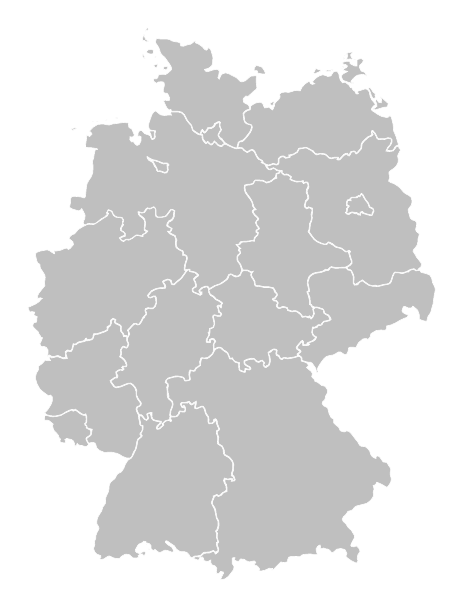
\begin{tikzpicture}[y=0.25pt, x=0.25pt, yscale=-1, xscale=1, inner sep=0pt, outer sep=0pt,every path/.style={fill,lightgray,draw=btdl@color@background!60,line width=.2pt}]
\path (259.7774,782.1800)arc(33.836:121.789:2.490) .. controls
   (254.3974,782.0400) and (252.3174,781.1300) ..
   (250.2174,780.4200)arc(290.251:228.635:7.140)arc(53.460:64.103:10.401) ..
   controls (239.3774,783.7600) and (237.4974,783.8900) ..
   (235.7974,781.9800)arc(314.975:307.442:35.814) .. controls (231.7274,779.5100)
   and (231.2574,780.0600) .. (230.7074,780.6700) .. controls (229.9974,780.3800)
   and (229.3374,780.1300) ..
   (228.7074,779.8400)arc(112.178:201.674:3.860)arc(18.003:-22.554:2.180)arc(334.737:272.456:6.570)
   -- (220.5074,771.7200) -- (219.9174,771.7200) .. controls (219.7274,770.5300)
   and (219.5474,769.3300) .. (219.3274,767.9000) -- (215.9474,767.1500) ..
   controls (215.6274,767.5200) and (215.2474,767.7800) ..
   (215.1374,768.1500)arc(17.816:93.379:2.730) .. controls (209.8374,770.1500)
   and (208.2974,771.6200) .. (207.1174,773.6600) .. controls (206.1174,775.3300)
   and (205.1174,776.9400) .. (204.2874,778.6600) .. controls (203.1774,780.9500)
   and (203.4774,781.8100) .. (205.5174,783.3100)arc(129.211:122.142:3.893) ..
   controls (209.0474,785.8800) and (210.2974,785.7000) ..
   (213.5474,783.1500)arc(239.333:272.143:6.540) .. controls (217.7074,782.2400)
   and (218.3374,783.0600) .. (219.1274,783.6500) .. controls (218.2774,785.3400)
   and (217.4974,786.8500) ..
   (216.4674,788.8600)arc(354.465:295.060:4.250)arc(303.355:223.734:2.570) ..
   controls (209.8474,786.6600) and (208.7674,787.3900) .. (207.6774,788.2700) --
   (209.1974,790.5100)arc(60.633:93.242:7.880) .. controls (203.2874,791.4000)
   and (201.6974,791.2600) ..
   (200.1074,791.1100)arc(88.143:176.878:2.910)arc(358.572:281.297:1.580)arc(284.904:278.615:47.855)
   .. controls (189.1974,785.5800) and (183.1174,789.2200) ..
   (182.4374,790.5700)arc(203.828:195.158:7.929) .. controls (178.0374,793.1000)
   and (174.3474,792.2400) .. (170.6974,790.6100)arc(110.769:144.548:2.000) ..
   controls (168.9774,788.3000) and (167.5974,788.3400) ..
   (166.0974,788.3400)arc(274.494:216.472:4.000) .. controls (160.5074,792.7700)
   and (157.2474,792.8900) .. (154.2674,793.6200) .. controls (153.2674,793.8700)
   and (152.5274,793.0800) .. (151.9874,791.9900) .. controls (152.7674,791.5900)
   and (153.5174,791.2100) .. (154.2274,790.8300) .. controls (154.4774,788.1400)
   and (154.3274,787.7000) .. (151.9574,787.2600)arc(99.661:148.274:9.740) ..
   controls (144.1174,781.0100) and (142.9974,779.3600) .. (143.1974,776.9500) ..
   controls (143.4874,776.6800) and (143.8874,776.3000) .. (144.2874,775.9500) ..
   controls (145.5474,774.8300) and (146.1274,773.4700) ..
   (145.3874,771.8800)arc(155.235:211.025:6.850) .. controls (146.6874,763.6500)
   and (147.6674,761.7500) .. (146.6874,759.5800) .. controls (147.4674,757.5100)
   and (148.1974,755.4100) .. (149.0574,753.3700)arc(206.329:222.493:8.622) ..
   controls (151.9274,749.5600) and (151.7174,747.7100) ..
   (150.5974,745.8300)arc(335.107:316.184:2.911) .. controls (148.0574,743.3300)
   and (147.9574,741.0400) .. (148.2074,738.7100) .. controls (148.5974,735.0000)
   and (149.4574,731.4500) ..
   (151.9974,728.5700)arc(42.365:6.879:19.690)arc(182.036:254.997:3.160) ..
   controls (160.9674,714.1400) and (161.2374,713.4500) .. (161.0674,711.7200) ..
   controls (160.9874,711.0000) and (160.8074,710.3100) ..
   (160.6674,709.6000)arc(166.733:204.870:8.630) .. controls (162.5074,701.3300)
   and (163.5874,698.5700) ..
   (164.9274,695.9900)arc(29.137:-3.187:8.000)arc(4.981:-4.981:10.999) ..
   controls (165.1774,686.5700) and (167.0974,684.2400) .. (168.3574,681.7400) ..
   controls (168.5874,681.3000) and (169.1874,681.0300) .. (169.6374,680.7400) ..
   controls (173.2674,678.3100) and (176.4674,675.5300) ..
   (177.3974,670.9700)arc(183.055:264.118:1.540) .. controls (180.7774,669.3102)
   and (182.2774,668.0502) .. (183.8474,666.9502)arc(57.441:11.303:7.730) ..
   controls (188.1474,657.6202) and (190.6274,654.0602) ..
   (193.0274,650.4602)arc(219.110:244.015:3.730) .. controls (195.5674,648.6702)
   and (196.9074,647.9802) ..
   (198.1674,647.1602)arc(56.198:4.960:5.910)arc(186.432:225.124:8.850)arc(43.553:9.698:7.280)
   .. controls (205.6574,631.5002) and (206.2774,629.3502) ..
   (206.6974,627.1502)arc(11.913:-0.599:19.549)arc(174.969:236.570:2.830) ..
   controls (210.0974,619.0202) and (211.7374,617.6302) ..
   (213.3774,616.2402)arc(50.421:-54.253:1.700)arc(306.411:298.420:17.000) ..
   controls (211.9074,611.6902) and (212.3874,611.2002) ..
   (212.8874,610.7402)arc(48.479:-4.607:6.200)arc(177.738:193.328:13.001) ..
   controls (215.7074,600.2702) and (215.2974,599.5202) .. (213.4874,599.3502) ..
   controls (212.8574,599.2902) and (212.2274,599.2802) .. (211.5774,599.2502) ..
   controls (211.8374,595.8402) and (210.9274,592.7102) .. (210.0674,589.5902) ..
   controls (209.9774,589.2802) and (209.6774,588.9502) .. (209.7474,588.7002) ..
   controls (210.0274,587.7002) and (210.1474,586.4202) .. (210.8074,585.7002) ..
   controls (211.6374,584.8802) and (212.6174,585.7002) .. (213.2474,586.4702) ..
   controls (214.2474,587.6802) and (215.1874,588.9902) .. (216.1374,590.2502) ..
   controls (216.2374,590.3702) and (216.2474,590.5502) ..
   (216.3274,590.6902)arc(155.473:81.184:3.490) .. controls (221.4974,592.3402)
   and (223.1474,590.5302) .. (223.0374,589.0502)arc(0.071:-30.581:11.000) --
   (225.4574,582.4402) .. controls (226.0674,584.8802) and (226.7274,587.1002) ..
   (227.1374,589.3602)arc(169.654:113.026:4.050) .. controls (232.0674,593.7202)
   and (234.8674,593.9702) .. (237.5974,594.5302) .. controls (238.5174,594.7202)
   and (239.4674,594.8502) .. (240.4874,595.0202)arc(4.146:78.226:3.000) ..
   controls (235.1074,598.5902) and (235.0374,601.3602) .. (234.0474,603.4802) ..
   controls (233.8474,603.8902) and (234.5274,605.0902) ..
   (235.0474,605.4002)arc(123.686:53.450:3.130) .. controls (239.4674,604.6702)
   and (240.1974,603.9302) .. (240.9674,603.2302) -- (245.2774,599.2302) ..
   controls (244.8274,598.4602) and (244.4274,597.8002) .. (244.0774,597.2302) ..
   controls (245.7174,593.7902) and (249.0774,593.4602) .. (252.0774,592.5702) ..
   controls (253.4574,592.1602) and (253.7974,593.7902) .. (255.0774,594.4102) ..
   controls (255.5174,594.0702) and (256.4774,593.7402) .. (256.6174,593.1902) ..
   controls (256.9474,591.8202) and (256.0674,590.8002) .. (254.8774,589.9902) ..
   controls (255.0974,589.2702) and (255.3174,588.5902) .. (255.5274,587.9002) ..
   controls (255.8774,587.9002) and (256.1974,587.8302) .. (256.5274,587.8302) --
   (260.8374,587.8302) .. controls (263.8374,587.8302) and (265.7074,586.1602) ..
   (267.1574,583.8302)arc(36.192:-6.009:1.280) .. controls (266.9574,581.6102)
   and (267.8074,580.8602) .. (268.7174,579.8302) -- (272.7774,580.7202) ..
   controls (274.4574,581.0902) and (276.1174,580.6502) .. (276.1574,579.4202) ..
   controls (276.2374,576.9202) and (277.5074,574.2402) ..
   (275.5974,571.9102)arc(324.801:278.654:2.790) .. controls (272.7374,570.8502)
   and (272.8274,571.8402) .. (272.9474,572.6702)arc(12.544:26.036:4.509) ..
   controls (271.1474,571.9402) and (269.9574,570.3902) ..
   (269.7074,567.9702)arc(260.014:277.520:30.531) -- (281.3474,565.6102) ..
   controls (281.1274,568.7802) and (283.2974,569.3502) .. (284.8974,570.3902) ..
   controls (285.6674,570.8802) and (286.2274,570.3302) ..
   (286.7674,569.8102)arc(225.461:233.238:37.120) .. controls (290.1674,568.6302)
   and (290.9174,570.8102) .. (289.5874,572.7302)arc(222.245:132.245:1.780) --
   (289.7084,575.2446) .. controls (289.7372,575.2708) and (289.7669,575.2960) ..
   (289.7974,575.3202) .. controls (290.6974,576.0202) and (291.5874,576.6402) ..
   (292.7974,576.0402) .. controls (294.7374,575.1102) and (296.6774,574.1702) ..
   (298.6774,573.4002) .. controls (301.0574,572.4802) and (302.3274,573.1402) ..
   (303.1174,575.6402) .. controls (303.9074,578.1402) and (304.4874,580.3902) ..
   (305.1674,582.7702)arc(168.848:124.148:6.670)arc(307.894:344.171:1.840)arc(-18.300:17.254:10.760)
   .. controls (308.1574,596.2102) and (308.4774,596.9402) .. (310.2274,597.4502)
   .. controls (314.2274,598.6202) and (317.0074,597.2902) .. (319.3874,592.8402)
   -- (318.0574,592.3802) .. controls (318.8274,591.1102) and (319.4874,590.8302)
   .. (320.0574,591.8702) .. controls (320.6274,592.9102) and (321.4674,593.9802)
   .. (320.8474,595.4402)arc(191.130:150.689:2.930) .. controls
   (322.2974,600.2202) and (323.5074,602.9802) ..
   (324.7274,605.8202)arc(61.819:72.709:5.998) .. controls (321.2174,606.6102)
   and (321.3974,606.6402) .. (320.9974,608.9402) .. controls (320.5974,611.2402)
   and (321.5974,613.3202) ..
   (322.5574,615.3202)arc(-25.604:14.115:5.000)arc(187.940:178.972:45.617)arc(168.589:122.020:2.000)arc(129.764:113.609:13.549)
   .. controls (329.1274,630.0402) and (330.0574,632.1202) .. (330.6074,634.3702)
   .. controls (331.1374,636.3702) and (331.8574,638.4602) .. (331.2474,640.6802)
   .. controls (330.9374,641.8202) and (331.6874,642.5902) ..
   (332.8474,642.9702)arc(290.798:309.637:22.520) .. controls (340.6374,647.6802)
   and (342.1374,648.6802) .. (342.5474,650.5502)arc(176.021:126.357:0.272) ..
   controls (345.1874,652.6502) and (344.7474,655.3702) .. (344.6574,657.9902) ..
   controls (344.6574,659.7502) and (344.5474,661.5002) ..
   (344.4774,663.2602)arc(2.897:29.802:12.140) .. controls (342.2974,669.8002)
   and (342.5874,671.3902) .. (342.4974,672.7502) -- (345.1574,673.7502) ..
   controls (345.6874,675.2102) and (346.1574,676.6102) .. (346.8074,678.3202) --
   (344.6474,680.0202) .. controls (344.4874,679.6002) and (344.3674,679.4402) ..
   (344.3974,679.3402) .. controls (345.1474,676.8802) and (344.6874,676.3402) ..
   (342.1974,676.5702)arc(273.402:266.598:2.106)arc(70.084:118.602:11.570) ..
   controls (332.0074,677.2302) and (331.5674,678.3802) ..
   (331.2274,679.5802)arc(190.051:130.641:3.000) .. controls (335.0674,685.5602)
   and (335.1474,689.5002) .. (335.2274,693.3802) .. controls (335.2274,695.1602)
   and (334.9374,695.2902) .. (333.2274,695.1002) .. controls (331.2274,694.8802)
   and (330.8274,695.5702) .. (329.6974,697.1002)arc(41.731:56.596:24.471) ..
   controls (324.6574,701.4402) and (323.9074,701.1302) ..
   (323.4474,700.8602)arc(126.023:135.833:12.229) -- (316.1874,701.8802) ..
   controls (317.0974,703.6502) and (316.1274,705.3702) .. (315.0674,707.0302) ..
   controls (313.0674,710.1602) and (313.0674,713.1702) ..
   (315.5174,716.0302)arc(321.141:357.624:17.510)arc(173.460:162.950:42.999)arc(158.607:147.171:18.831)arc(326.829:348.753:4.800)arc(-3.289:3.289:50.113)arc(9.678:22.892:12.087)
   .. controls (322.3074,748.4502) and (322.0174,749.4502) .. (321.6774,750.5102)
   .. controls (319.3374,751.9502) and (319.2074,752.6202) ..
   (320.7774,755.1202)arc(-26.129:3.799:3.000) .. controls (321.0774,758.3102)
   and (320.9874,759.9902) .. (321.0074,761.6402)arc(182.452:140.788:9.230) --
   (320.8774,768.9902)arc(177.177:170.576:43.150)arc(163.159:153.711:24.610) ..
   controls (323.9774,780.4102) and (323.4774,781.5102) ..
   (320.7574,782.5602)arc(245.587:237.390:6.448) .. controls (318.5774,780.0002)
   and (315.3374,779.4502) .. (313.2474,781.7702)arc(41.515:95.040:3.000) ..
   controls (308.4974,782.7702) and (306.2674,782.8902) ..
   (304.0274,782.9302)arc(272.230:219.806:3.370) .. controls (300.2174,785.4102)
   and (298.9774,786.5602) .. (297.7874,787.7402) .. controls (296.4374,789.0802)
   and (295.4774,789.1302) .. (293.5774,788.3202) .. controls (292.1574,787.7102)
   and (290.6674,787.4902) ..
   (289.3074,788.6402)arc(49.732:56.911:19.120)arc(55.240:145.240:3.370) --
   (282.6974,789.2229) .. controls (282.6627,789.1729) and (282.6294,789.1220) ..
   (282.5974,789.0702)arc(150.322:164.607:10.492)arc(345.584:283.228:4.610)arc(103.854:110.941:25.435)arc(290.811:253.545:7.000)arc(72.238:112.915:2.880)
   .. controls (266.8374,781.0502) and (265.0474,779.8602) ..
   (263.2974,778.6202)arc(120.555:179.217:3.540) .. controls (261.5574,774.5602)
   and (260.7674,774.1202) .. (260.0474,773.6202) .. controls (257.9274,772.2002)
   and (255.7674,770.8202) .. (253.6574,769.3902) .. controls (252.5274,768.6302)
   and (251.4574,767.8002) ..
   (250.3374,767.0502)arc(302.988:285.355:4.541)arc(293.103:204.822:1.400)arc(213.117:132.633:1.560)arc(139.358:114.599:22.100)arc(290.748:325.176:3.900)arc(330.682:336.969:59.736)
   -- cycle(223.2874,778.1200)arc(226.602:168.449:0.820) .. controls
   (223.4874,779.7300) and (224.1074,779.4600) .. (224.8474,779.0000) .. controls
   (224.5974,777.9400) and (224.0574,777.6900) .. (223.2874,778.1200) -- cycle;



\path (551.7774,647.5800) -- (551.7774,644.5800) .. controls (554.4274,643.5800)
   and (555.5874,643.7800) .. (557.1574,645.6700)arc(318.405:331.539:22.851) ..
   controls (561.7974,653.2200) and (562.0674,653.4800) ..
   (565.6574,653.1400)arc(84.522:77.298:10.047) --
   (572.7974,662.0400)arc(-33.887:24.673:2.800)arc(12.610:23.044:13.112) ..
   controls (571.2874,668.5700) and (571.6874,669.7900) .. (572.2874,671.4200) ..
   controls (574.1674,676.1400) and (574.4574,680.8900) ..
   (570.9774,685.2000)arc(218.722:212.204:31.532)arc(21.050:128.968:1.530) ..
   controls (564.7874,687.7600) and (563.0174,686.7600) .. (561.3574,685.7000) ..
   controls (558.8074,683.9600) and (555.9474,683.0300) .. (552.8174,681.9400) ..
   controls (552.5974,685.1100) and (550.3474,686.2200) .. (547.5874,686.8600) ..
   controls (547.8774,687.3800) and (548.0474,687.7100) ..
   (548.2474,688.0400)arc(-36.101:22.256:4.680)arc(203.238:194.332:19.999)arc(197.992:164.873:3.510)
   .. controls (548.9774,700.3700) and (547.8874,703.0300) ..
   (546.3574,705.0900)arc(35.783:58.162:26.999)arc(54.122:92.743:6.310)arc(277.628:235.341:7.770)arc(53.771:90.133:3.000)
   .. controls (524.9274,715.0600) and (523.1074,716.6300) ..
   (521.0974,717.7000)arc(233.026:212.512:4.590) .. controls (519.2474,719.8400)
   and (518.5474,720.8000) ..
   (517.8274,721.7600)arc(32.520:93.313:2.930)arc(268.574:260.243:9.890) ..
   controls (511.7574,723.3900) and (510.1674,723.9400) .. (509.6874,726.3700) ..
   controls (509.4674,727.4900) and (508.3574,728.4900) ..
   (507.4874,729.3700)arc(47.390:53.694:32.623) .. controls (502.1874,733.7300)
   and (502.0874,736.6500) ..
   (504.5174,738.9800)arc(133.515:125.773:33.662)arc(303.795:352.718:7.000)arc(180.092:93.248:3.000)arc(282.415:327.316:3.000)
   .. controls (517.4874,753.8098) and (519.0474,756.5998) .. (520.7774,759.3198)
   .. controls (521.3974,760.3198) and (521.0174,761.0998) .. (520.5574,761.9698)
   .. controls (518.8707,765.1432) and (517.2041,768.3298) .. (515.5574,771.5298)
   .. controls (514.6574,773.2998) and (515.0774,774.4098) ..
   (516.8274,775.0898)arc(107.691:51.363:7.110) .. controls (527.1574,775.2098)
   and (527.2074,778.9898) ..
   (528.7474,781.8698)arc(31.680:38.250:15.228)arc(222.495:179.496:12.070)arc(186.873:158.518:3.211)
   .. controls (526.1674,795.6798) and (526.1674,795.9498) .. (524.1974,798.0298)
   .. controls (523.9274,798.3098) and (523.6274,798.5598) ..
   (523.2974,798.8798)arc(106.566:125.355:23.370) .. controls (514.6174,794.3698)
   and (512.8574,793.1298) .. (511.0774,791.9098) .. controls (507.5274,789.4798)
   and (507.3574,788.6898) .. (509.7974,785.0798) .. controls (509.0074,783.4398)
   and (508.2074,781.7098) ..
   (507.3474,780.0098)arc(334.775:298.768:2.220)arc(294.616:248.800:14.650)arc(250.019:205.377:1.780)
   .. controls (493.4474,781.5798) and (491.7374,782.1498) .. (490.1774,782.9398)
   .. controls (489.5574,783.2498) and (488.8974,783.5198) .. (487.9974,783.9398)
   .. controls (486.8574,782.6098) and (485.6774,781.3398) ..
   (484.6174,779.9398)arc(329.408:270.922:2.770)arc(90.529:103.904:13.330)arc(108.252:115.791:25.762)
   -- (472.0574,778.3098) .. controls (471.2974,777.0798) and (470.8574,775.9798)
   .. (471.4974,774.6598)arc(31.232:-58.768:1.460) -- (471.0060,772.6543) ..
   controls (470.9674,772.6310) and (470.9279,772.6095) .. (470.8874,772.5897) ..
   controls (470.4274,772.4097) and (469.5674,772.8497) ..
   (469.0574,773.2197)arc(229.621:222.349:22.693) .. controls (464.7674,777.3597)
   and (464.4074,779.3597) .. (465.6174,782.2997) .. controls (466.1374,783.5297)
   and (466.5174,784.8197) .. (467.0574,786.3697)arc(75.480:87.409:10.997) ..
   controls (462.4374,786.5397) and (459.9774,786.8797) ..
   (457.7974,785.6097)arc(299.398:249.399:1.080) .. controls (455.0174,786.3497)
   and (453.1074,785.8797) .. (451.2074,785.8797)arc(270.415:255.115:17.000) ..
   controls (444.8974,786.9397) and (442.9074,787.3697) .. (442.3774,789.4497) ..
   controls (437.9174,789.3297) and (433.6974,789.2597) .. (429.4874,789.0997) ..
   controls (426.3474,788.9897) and (424.6574,790.3297) ..
   (424.1374,793.5297)arc(189.855:180.430:6.111) .. controls (423.9874,796.9997)
   and (423.9974,796.9997) .. (421.4574,797.5897) .. controls (418.2374,798.3497)
   and (416.5574,798.2197) .. (414.3474,797.0097) .. controls (413.8874,797.4197)
   and (413.3474,797.8697) .. (412.8674,798.3597) .. controls (410.6174,800.6197)
   and (408.3674,802.8797) .. (406.1574,805.1797)arc(224.647:210.490:13.310) ..
   controls (403.1574,809.4697) and (403.2574,809.5197) .. (400.7174,809.4197) --
   (402.4574,806.6397)arc(302.608:246.845:5.450) .. controls (395.1574,807.1097)
   and (393.0274,808.2197) .. (390.8674,809.2197) .. controls (388.2174,810.4897)
   and (385.5074,809.9097) .. (382.6074,809.9197) .. controls (383.9174,807.2197)
   and (383.8874,807.1797) .. (382.0474,805.0497) .. controls (380.5674,803.3397)
   and (379.0474,801.6997) .. (376.5574,801.6397) .. controls (376.2174,801.6397)
   and (375.8874,801.2997) .. (375.2374,800.9497) --
   (378.0174,798.2197)arc(340.246:332.495:5.167) .. controls (376.3674,795.3897)
   and (375.9574,795.2397) .. (373.4474,795.9697)arc(257.522:248.623:1.550) ..
   controls (370.1474,797.9197) and (367.2174,796.9397) .. (364.3774,795.5297) ..
   controls (364.0174,795.3597) and (363.5174,795.2197) .. (363.3774,794.9197) ..
   controls (363.0274,794.1897) and (362.7774,793.4697) .. (361.7974,793.3697) ..
   controls (359.8974,793.1597) and (358.0174,792.8597) .. (356.1074,792.7597) ..
   controls (355.7174,792.7597) and (355.2074,793.3797) ..
   (354.9274,793.8197)arc(210.830:203.783:19.684)arc(81.237:122.989:9.428) ..
   controls (347.5274,793.3397) and (347.7874,792.2297) .. (348.0874,790.8797) ..
   controls (346.9974,790.8797) and (346.2274,790.8197) ..
   (345.4674,790.8797)arc(270.736:173.239:1.700) .. controls (343.7574,795.0197)
   and (343.6774,797.2697) .. (343.8774,799.4797) .. controls (343.9974,800.6497)
   and (344.0374,802.1297) .. (345.7474,802.4797)arc(287.194:341.016:1.000) ..
   controls (346.5074,804.7897) and (347.2474,806.5397) .. (345.9974,808.1097) ..
   controls (343.4474,811.3897) and (340.9974,814.7897) .. (338.3774,817.9597) ..
   controls (335.5774,821.3097) and (331.7874,822.7597) ..
   (327.0774,822.9597)arc(197.721:209.120:44.333) .. controls (330.8174,814.4697)
   and (331.2774,814.1097) .. (331.3374,813.6797)arc(12.806:-24.794:3.120) ..
   controls (330.1274,810.4397) and (328.6374,810.8397) .. (327.3274,810.8097) ..
   controls (326.2174,810.8097) and (325.6674,811.5997) ..
   (325.5674,812.6997)arc(19.496:31.986:2.858) -- (321.9274,814.3297) .. controls
   (321.5174,813.1597) and (321.1874,812.1897) ..
   (320.8574,811.2297)arc(158.215:232.019:1.820) .. controls (322.6974,807.8297)
   and (322.6674,807.5597) ..
   (321.6174,806.0197)arc(325.540:317.670:29.562)arc(315.919:263.305:5.210) ..
   controls (313.3974,799.1497) and (311.6174,797.2297) .. (313.1774,794.2897) ..
   controls (309.7774,796.8197) and (306.5374,797.6497) .. (302.9074,795.1297) ..
   controls (302.9574,794.4597) and (303.0274,793.6797) .. (303.0474,792.9197) ..
   controls (303.0474,791.2597) and (302.5974,790.5297) ..
   (301.1474,789.9797)arc(292.958:218.423:2.940) .. controls (296.6974,792.0297)
   and (295.8774,793.2797) .. (294.9074,794.5897)arc(100.581:119.623:23.659) ..
   controls (288.6674,791.0697) and (289.5574,790.3897) ..
   (290.4274,789.7397)arc(234.301:302.103:2.000)arc(121.405:40.807:5.000) ..
   controls (300.3974,787.2997) and (301.5674,785.5097) .. (303.2074,784.7697) ..
   controls (304.8474,784.0297) and (306.9574,784.3897) ..
   (308.8674,784.2897)arc(265.101:271.543:21.277)arc(100.995:31.393:2.930) ..
   controls (315.2574,781.2997) and (316.6974,782.1297) .. (318.1174,782.2297) ..
   controls (318.5174,783.4897) and (318.8874,784.6697) .. (319.2374,785.7897) ..
   controls (319.5074,785.8697) and (319.7574,785.9897) .. (319.7874,785.9397) ..
   controls (320.8374,784.5897) and (322.4974,783.9397) ..
   (323.6774,782.8697)arc(47.807:-23.494:3.870) .. controls (324.0974,777.1397)
   and (323.4774,775.8297) .. (323.0274,774.4597)arc(163.226:173.336:18.719) ..
   controls (322.1574,769.8797) and (323.6174,769.7497) .. (324.1674,768.9297) ..
   controls (324.2974,768.7297) and (324.4574,768.5497) .. (324.5874,768.3697) ..
   controls (321.2474,761.1597) and (322.3174,760.0297) .. (322.7274,755.4597) ..
   controls (322.1074,754.5597) and (321.5674,753.7697) .. (320.9474,752.8397) --
   (322.7674,751.8397) .. controls (323.3974,750.1697) and (324.0274,748.8397) ..
   (324.4274,747.3897)arc(15.415:1.299:14.560) .. controls (324.9474,742.0997)
   and (324.8274,740.3397) .. (324.6974,738.5897)arc(3.827:-35.492:2.070) ..
   controls (321.8974,735.0797) and (321.7874,732.0097) .. (321.1874,729.1697) ..
   controls (320.6574,726.6797) and (320.4174,724.1697) ..
   (320.0574,721.5997)arc(352.999:321.112:5.930)arc(143.604:150.566:47.278)arc(144.487:209.340:3.810)arc(28.085:22.190:27.928)
   .. controls (317.2174,705.7897) and (317.7274,704.4697) .. (318.4074,702.7797)
   -- (321.6974,700.9997) -- (323.6974,702.8197)arc(93.188:40.700:5.370) ..
   controls (329.2174,699.6297) and (331.2174,699.0497) .. (331.6174,696.9597) ..
   controls (331.6674,696.6897) and (332.7074,696.3397) ..
   (333.1974,696.4597)arc(105.041:44.685:3.390)arc(6.956:-16.260:25.430)arc(338.655:319.677:11.479)
   .. controls (332.3974,680.1897) and (332.3774,680.1197) .. (333.6174,677.5497)
   .. controls (336.7874,679.5497) and (340.1474,678.2597) .. (343.8374,677.7497)
   -- (342.3874,680.7497)arc(118.559:47.589:4.000)arc(49.620:29.435:6.770) ..
   controls (348.9674,677.4297) and (348.0174,676.9897) ..
   (347.5874,676.3597)arc(152.817:170.532:5.370) .. controls (346.9174,674.2597)
   and (346.7974,673.6997) .. (346.6274,673.0197) -- (345.2274,672.3897) ..
   controls (343.9674,671.8497) and (343.3774,670.8797) .. (344.0474,669.8097) ..
   controls (346.2074,666.3397) and (345.8974,662.4597) .. (346.1274,658.6597) ..
   controls (346.1774,657.6597) and (346.1274,656.7497) ..
   (346.1774,655.7897)arc(8.017:-46.393:5.790)arc(126.428:152.720:1.559) ..
   controls (342.2874,646.1297) and (338.4074,644.5797) .. (334.9774,642.5597) ..
   controls (334.4374,642.2397) and (333.8174,642.0297) ..
   (333.2474,641.7497)arc(123.846:143.816:0.999)arc(3.878:-33.830:19.220) ..
   controls (329.4274,628.9697) and (328.5874,628.7697) .. (327.9374,628.5097) ..
   controls (323.7874,626.5097) and (323.6074,626.2297) ..
   (323.8574,621.6297)arc(174.833:198.446:4.650) .. controls (325.2074,617.6197)
   and (324.5074,615.7397) .. (323.4174,613.9297)arc(146.854:200.856:6.790) ..
   controls (323.2674,607.7297) and (323.8874,607.6897) .. (324.4774,607.5597) ..
   controls (325.9074,607.2397) and (326.4174,606.4697) .. (325.8874,605.1297) ..
   controls (324.8174,602.3997) and (323.6174,599.7297) ..
   (322.4874,597.0197)arc(150.826:189.748:1.690) .. controls (323.1474,594.0797)
   and (321.9974,592.6697) .. (321.2474,591.2597) .. controls (320.4974,589.8497)
   and (319.1874,589.6497) .. (317.8974,590.7597)arc(226.858:218.962:14.079) --
   (317.5774,593.7997) .. controls (315.4274,596.7297) and (313.1074,597.3797) ..
   (309.9574,595.9097) .. controls (310.4674,593.0397) and (310.8974,590.1397) ..
   (309.8074,587.2697) .. controls (309.6174,586.7897) and (309.3374,586.1397) ..
   (308.9274,585.9497) .. controls (307.3574,585.2297) and (306.8774,583.8197) ..
   (306.4574,582.3597) .. controls (305.7974,580.1397) and (305.0774,577.9397) ..
   (304.5874,575.6797)arc(343.561:303.287:6.800)arc(296.463:246.973:2.390) ..
   controls (297.6374,572.6597) and (295.5074,573.5697) .. (293.4174,574.5197) ..
   controls (292.4174,574.9797) and (291.5274,575.4697) .. (290.6674,574.2997) ..
   controls (292.0874,571.2997) and (292.0474,568.0797) .. (292.0374,564.7097) ..
   controls (288.8874,565.0997) and (287.8374,568.0597) .. (285.4774,569.2897) ..
   controls (284.2773,568.4497) and (282.7773,568.1197) .. (282.7773,566.1197) ..
   controls (282.7773,564.8597) and (280.7773,564.3397) ..
   (279.7773,565.4097)arc(47.082:96.048:3.510) .. controls (274.7773,566.4097)
   and (272.5473,566.5564) .. (270.3273,566.7697) .. controls (268.6073,566.9397)
   and (268.1673,567.5097) ..
   (268.7273,569.1297)arc(157.209:149.969:39.527)arc(160.044:70.045:1.750) --
   (273.1895,574.6474) .. controls (273.2293,574.6329) and (273.2686,574.6170) ..
   (273.3073,574.5997) .. controls (273.8873,574.3397) and (274.2473,573.5997) ..
   (274.7773,572.9597) .. controls (276.7773,574.7797) and (274.3873,577.0997) ..
   (275.2173,579.3097) .. controls (272.6373,580.2397) and (270.4473,578.0397) ..
   (267.9273,578.8997) .. controls (267.1573,580.1497) and (265.4873,581.2097) ..
   (266.0973,583.2797) .. controls (265.2073,584.4797) and (264.5473,586.0597) ..
   (262.8673,586.2797)arc(83.236:90.710:49.400) .. controls (255.2073,586.6197)
   and (254.5573,585.8097) .. (254.7173,584.4897) .. controls (255.1573,581.0397)
   and (255.0873,577.4897) .. (257.2073,574.3997) .. controls (259.2073,571.4697)
   and (258.8873,568.2197) .. (257.7773,565.0197)arc(341.295:296.009:1.730) ..
   controls (254.6073,563.2997) and (253.4473,561.2597) .. (251.8973,559.7397) ..
   controls (250.9873,558.8697) and (251.1973,558.4797) .. (252.7173,557.6697) ..
   controls (251.2773,555.9697) and (251.3073,553.8997) .. (251.2073,551.8497) ..
   controls (251.1373,550.3297) and (250.9573,548.8497) .. (250.8773,547.3097) ..
   controls (250.8073,546.0897) and (250.5273,544.9897) .. (251.5173,543.7397) ..
   controls (252.0973,542.9997) and (251.5173,541.3097) .. (251.4373,540.0397) ..
   controls (251.3373,538.2797) and (249.6573,538.5097) .. (248.7373,538.0397) ..
   controls (248.6273,537.7097) and (248.5173,537.5497) .. (248.5473,537.4197) ..
   controls (249.8173,532.1097) and (249.4873,532.9597) ..
   (254.2173,531.6497)arc(78.394:69.872:33.722) .. controls (263.6273,528.2797)
   and (267.9773,530.0597) .. (272.3873,530.8797) .. controls (272.9073,530.9797)
   and (273.4373,531.7797) .. (273.6973,532.3797) .. controls (275.3273,536.0297)
   and (274.4973,536.2797) .. (279.5673,535.3797) -- (281.2073,535.0897) ..
   controls (283.4373,534.6897) and (283.9573,533.8397) .. (283.4173,531.5597) ..
   controls (283.0673,530.0897) and (282.7173,528.5597) ..
   (282.4973,527.1197)arc(167.821:213.902:8.000) .. controls (285.2273,521.2097)
   and (286.7773,521.4797) ..
   (288.3473,521.6797)arc(106.789:4.535:1.890)arc(197.046:207.225:10.771)arc(199.075:260.235:3.340)
   .. controls (297.7073,515.1097) and (299.5073,512.2097) .. (298.5773,508.6297)
   .. controls (298.0673,506.6297) and (299.1573,505.1197) .. (299.6373,503.4197)
   .. controls (299.8273,502.7597) and (302.1273,502.3597) .. (302.9173,502.8397)
   .. controls (305.8073,504.5697) and (308.1273,503.4997) ..
   (310.6073,501.7697)arc(53.551:41.611:33.211)arc(43.469:11.075:8.450) ..
   controls (318.4173,490.4297) and (320.8673,488.6097) .. (323.3473,488.0897) ..
   controls (326.4773,487.4297) and (328.6673,488.0897) ..
   (330.2373,491.0297)arc(147.045:103.096:4.000) .. controls (336.8073,493.7497)
   and (337.7473,497.2097) .. (338.9673,500.4797)arc(346.733:357.233:3.918) ..
   controls (339.5073,503.9197) and (339.8773,504.1897) ..
   (342.6573,504.0597)arc(85.926:79.302:9.425) .. controls (345.3173,508.3597)
   and (349.4673,508.9797) .. (353.3973,510.1997) .. controls (353.2773,511.3797)
   and (353.2573,512.4797) ..
   (353.0773,513.5597)arc(187.608:159.989:12.410)arc(168.604:100.484:2.380) ..
   controls (357.3073,521.7497) and (358.9273,522.4797) .. (360.6173,523.0397) ..
   controls (362.6173,523.7097) and (363.4373,523.0397) .. (363.2873,520.8897) ..
   controls (363.2873,520.2797) and (363.1673,519.6697) .. (363.0773,518.7397) --
   (366.7173,519.4897)arc(104.174:94.663:12.899)arc(96.323:11.623:2.120) ..
   controls (371.4873,516.7797) and (371.1373,515.5697) .. (369.8173,515.2197) ..
   controls (367.7473,514.6297) and (366.2073,513.2197) .. (364.4173,512.2197) ..
   controls (362.4173,511.0797) and (361.5673,509.5597) .. (362.2373,507.0997) ..
   controls (366.0673,505.0997) and (370.1473,503.4297) ..
   (374.8073,504.0997)arc(282.718:314.192:3.250)arc(320.955:336.981:5.149)arc(146.678:38.025:6.000)
   .. controls (388.7173,507.2397) and (388.7173,507.2397) .. (389.8973,509.6497)
   .. controls (389.5573,510.0197) and (389.1773,510.4097) ..
   (388.8173,510.8297)arc(224.953:142.112:1.840)arc(143.915:130.651:17.678)arc(133.149:17.167:1.220)arc(200.256:276.046:2.530)
   .. controls (397.0273,514.0897) and (397.4473,513.5297) .. (397.6873,512.6397)
   .. controls (398.1473,510.8697) and (398.7673,509.1297) ..
   (399.1873,507.3497)arc(10.222:-10.222:6.621) .. controls (399.0073,503.4897)
   and (398.7173,501.9997) .. (398.4773,500.5097) .. controls (398.2673,499.2697)
   and (398.2673,497.9897) .. (397.0673,497.0897) .. controls (396.6873,496.8097)
   and (396.7273,495.9597) .. (396.5673,495.3097) .. controls (398.9073,494.4297)
   and (400.9073,493.3797) ..
   (402.1573,491.2597)arc(216.397:263.401:2.000)arc(262.960:300.136:6.660)arc(193.820:186.745:37.227)
   .. controls (406.7473,498.1497) and (407.4373,498.9497) ..
   (409.6673,499.5997)arc(105.338:89.583:3.091)arc(149.097:143.012:46.899)arc(140.625:35.903:2.710)arc(36.338:25.893:7.122)
   .. controls (418.5573,502.5997) and (418.7873,502.4897) .. (418.8673,502.5997)
   .. controls (420.2373,504.0497) and (421.8673,503.9997) .. (423.6873,503.6497)
   .. controls (428.0673,502.7997) and (432.6073,502.8997) .. (436.8173,501.1697)
   .. controls (437.4073,500.9197) and (437.9973,500.6697) .. (438.5973,500.4597)
   .. controls (439.5173,500.1497) and (440.4573,499.1197) .. (441.4273,500.1697)
   .. controls (442.5473,501.3897) and (444.4273,502.2297) ..
   (443.6573,504.4997)arc(191.503:179.239:11.001) .. controls (445.3773,507.3997)
   and (447.2573,507.9897) .. (449.1573,508.4897)arc(283.247:343.281:7.000) --
   (451.2573,516.1397)arc(152.989:110.532:6.220)arc(296.634:339.708:10.620)arc(221.204:165.895:4.920)
   .. controls (459.0673,530.7797) and (459.2273,531.9097) .. (461.0873,532.1397)
   .. controls (462.6473,532.3397) and (463.2873,533.8297) .. (463.3173,536.0797)
   .. controls (463.4173,536.1797) and (463.5273,536.3697) .. (463.6373,536.3797)
   .. controls (466.3473,536.5497) and (468.2573,537.9397) .. (470.1773,539.8097)
   .. controls (471.8873,541.4797) and (473.9673,543.0097) ..
   (476.6873,542.9797)arc(266.545:311.668:2.110) .. controls (480.1373,545.8297)
   and (482.2173,548.1297) .. (481.8673,551.5097)arc(11.550:34.940:4.000) ..
   controls (479.6573,555.7697) and (477.8873,558.4497) ..
   (477.9373,561.8597)arc(9.568:50.205:2.890)arc(50.262:58.612:18.066) ..
   controls (473.2973,566.2197) and (473.0473,566.6797) .. (473.8973,568.3197) ..
   controls (475.0673,570.5797) and (476.2773,572.9497) .. (479.2873,573.1897) ..
   controls (481.6473,573.3697) and (482.2873,574.8497) .. (482.3673,576.9197) ..
   controls (482.4973,581.3297) and (484.9373,584.9197) .. (486.8073,588.6497) ..
   controls (487.2673,589.5597) and (488.9273,589.8797) .. (490.3673,590.6497) ..
   controls (490.3673,591.2697) and (490.7773,592.3397) .. (490.4473,593.0997) ..
   controls (489.4473,595.5297) and (491.0173,596.8597) .. (492.4473,598.1697) ..
   controls (493.9973,599.6497) and (495.7873,600.8997) ..
   (497.4473,602.2297)arc(304.503:355.549:2.880) .. controls (498.9873,607.0597)
   and (500.3073,608.3197) .. (502.8873,608.7497) .. controls (504.1573,608.9597)
   and (505.4173,609.1497) .. (506.6773,609.2997) .. controls (508.3573,609.4897)
   and (508.3673,609.4697) .. (508.8673,607.7697) .. controls (511.8673,607.5397)
   and (514.0173,609.1697) .. (515.7373,611.4097) .. controls (518.1673,614.5697)
   and (520.5473,617.7897) .. (522.9773,620.9597)arc(144.148:132.400:15.121) ..
   controls (526.1873,624.2697) and (527.4073,625.1497) ..
   (527.1173,626.9997)arc(176.091:128.510:1.680) .. controls (529.5873,629.7297)
   and (531.3773,631.3897) ..
   (534.1373,630.2797)arc(256.886:300.736:2.710)arc(299.934:327.577:18.400)arc(332.183:353.473:14.760)arc(171.885:118.131:4.050)
   .. controls (547.2973,645.5197) and (548.2973,646.3597) ..
   (549.4073,646.9897)arc(108.272:99.697:16.334) -- cycle;



\path (515.9774,275.3300)arc(350.441:342.637:14.203) .. controls
   (514.8774,271.9100) and (515.3374,271.0700) ..
   (517.0074,271.0100)arc(266.102:275.097:30.479) .. controls (523.7074,271.2800)
   and (525.2774,270.9800) .. (526.2974,269.2600) .. controls (527.1474,269.3100)
   and (528.0174,269.6000) .. (528.6274,269.3200) .. controls (529.2374,269.0400)
   and (529.3474,268.1700) .. (529.6874,267.5600) .. controls (530.0274,266.9500)
   and (530.3774,266.3300) .. (530.8474,265.4800)arc(317.486:325.490:13.000) ..
   controls (532.9774,268.7100) and (533.8974,270.5900) ..
   (534.9774,272.3700)arc(152.106:136.788:16.001)arc(314.350:348.224:14.540) ..
   controls (541.6374,283.7400) and (541.7774,284.2000) .. (541.8874,284.6300) --
   (547.0074,287.2500) .. controls (547.9074,287.7000) and (548.4174,288.3600) ..
   (547.9474,289.3600)arc(20.633:38.133:12.259)arc(232.011:148.184:2.220)arc(93.477:100.872:22.350)
   .. controls (540.1974,294.4900) and (537.6774,293.7600) .. (535.1474,293.0000)
   .. controls (533.0874,292.3700) and (533.0874,292.3500) .. (531.9974,290.4800)
   .. controls (528.5574,291.0800) and (528.3174,291.3500) .. (528.1074,294.8600)
   .. controls (526.1074,294.9100) and (525.6374,292.7600) .. (523.9974,292.0800)
   .. controls (523.0874,292.6100) and (522.2474,292.2900) ..
   (521.1474,291.8100)arc(295.740:230.585:7.800) .. controls (510.9774,294.2000)
   and (510.9274,294.1300) ..
   (509.0474,292.5100)arc(43.793:28.078:6.731)arc(25.997:-17.968:2.290) ..
   controls (509.4774,288.0000) and (509.8974,287.1000) .. (510.8074,286.1100) ..
   controls (511.7174,285.1200) and (512.4674,283.9800) .. (513.4674,282.6800) --
   (510.0574,280.6300) .. controls (510.1174,279.4000) and (510.1274,277.9600) ..
   (510.2674,276.5400) .. controls (510.4574,274.6600) and (511.1774,274.2700) ..
   (512.9774,274.7700)arc(103.774:97.373:27.332) -- cycle;



\path (509.9274,207.6100) .. controls (510.2774,208.3100) and
   (510.6074,208.8500) .. (510.8474,209.4500)arc(161.418:71.418:1.790) --
   (513.1145,210.5763) .. controls (513.1390,210.5680) and (513.1633,210.5593) ..
   (513.1874,210.5500)arc(61.326:6.946:2.340)arc(178.219:237.180:4.590) ..
   controls (517.8274,203.9000) and (519.2474,204.2400) .. (520.5874,204.3000) ..
   controls (520.7574,204.4800) and (520.9274,204.5700) .. (520.9774,204.7000) ..
   controls (522.4274,208.3200) and (523.1574,208.4900) .. (525.7874,205.7000) ..
   controls (527.4174,203.9600) and (528.9574,202.1200) ..
   (530.5374,200.3200)arc(44.138:-12.708:2.870) .. controls (530.6374,194.4200)
   and (531.8774,191.7700) .. (534.2774,189.5600) .. controls (536.2774,187.6400)
   and (538.2774,185.6900) .. (540.3974,183.8300)arc(224.879:260.664:3.770) ..
   controls (544.8374,182.7200) and (546.0874,181.0600) .. (547.6974,179.4800) ..
   controls (546.0074,178.2500) and (545.6974,176.7000) .. (546.4574,174.4200) ..
   controls (548.3774,176.8700) and (550.7674,178.4900) ..
   (551.5674,181.4200)arc(161.746:154.651:34.813)arc(161.276:76.330:2.290) ..
   controls (558.6674,185.9100) and (561.4174,186.7000) .. (564.1774,186.6000) ..
   controls (565.2674,186.6000) and (566.4274,186.8000) .. (567.1774,185.6000) ..
   controls (567.3474,185.3300) and (568.0374,185.3000) .. (568.4874,185.2800) ..
   controls (569.2074,185.2800) and (569.9274,185.2800) .. (570.6374,185.3400) ..
   controls (573.6374,185.4900) and (573.9974,185.3400) ..
   (573.9174,189.1500)arc(3.085:40.126:8.550)arc(38.028:43.893:49.056) ..
   controls (566.6274,200.1600) and (566.3274,200.6200) .. (565.9274,203.4100) ..
   controls (569.4774,203.9600) and (573.0374,204.4100) ..
   (576.4774,203.2700)arc(64.312:16.470:5.100) .. controls (579.8674,197.3900)
   and (581.8374,196.6100) .. (584.1574,195.9400) .. controls (585.1574,197.7600)
   and (584.1574,200.7400) .. (587.3274,201.3600) .. controls (586.9074,203.7100)
   and (585.5274,205.4100) .. (584.2274,207.0800) .. controls (582.5974,209.1500)
   and (582.5974,211.2300) ..
   (583.5274,213.5400)arc(-23.748:1.128:5.800)arc(4.401:12.323:32.849)arc(10.055:45.689:7.690)
   .. controls (578.8274,226.9300) and (576.7674,229.5100) ..
   (573.6274,230.8000)arc(243.332:229.818:5.092) .. controls (570.1074,233.3000)
   and (569.8674,233.9600) .. (570.5674,236.9100)arc(167.127:161.312:14.137) ..
   controls (571.7274,240.4500) and (572.0474,242.3900) .. (570.3874,244.5000) ..
   controls (568.9774,246.3000) and (570.0274,247.8100) ..
   (572.3274,248.4500)arc(286.055:296.948:33.629) .. controls (579.9174,251.6100)
   and (581.3374,252.7900) ..
   (582.9274,253.7400)arc(301.688:328.761:19.289)arc(144.872:116.187:17.580) ..
   controls (596.9074,266.3600) and (597.9874,266.6600) .. (598.9074,267.2300) ..
   controls (601.5974,268.8400) and (603.8174,270.8000) ..
   (603.5974,274.3600)arc(183.252:174.144:16.630) .. controls (603.9674,280.3500)
   and (602.4774,282.8200) .. (599.9374,284.8100) .. controls (598.5274,285.9000)
   and (597.5374,289.1600) ..
   (598.4074,290.6700)arc(333.218:352.558:13.860)arc(168.194:162.097:49.506)arc(166.933:96.021:3.670)arc(278.653:287.253:27.371)arc(-79.554:5.158:2.590)
   .. controls (610.4274,308.4000) and (610.4274,310.0900) ..
   (610.2774,311.7300)arc(8.517:32.092:5.220)arc(207.556:143.571:5.490)arc(138.709:115.193:3.469)
   .. controls (614.2874,321.7700) and (615.2574,323.3800) .. (613.6374,326.2600)
   .. controls (612.2374,328.7500) and (612.2274,331.2600) .. (612.3374,333.7700)
   .. controls (612.4974,337.7700) and (610.6674,340.7700) .. (608.0674,343.5500)
   .. controls (607.5174,344.1300) and (606.9074,344.6500) .. (606.3474,345.2200)
   .. controls (604.7474,346.8900) and (604.6574,349.0000) ..
   (606.4974,350.3600)arc(309.524:339.804:7.580) .. controls (609.2074,354.4500)
   and (609.6274,355.3100) .. (609.9674,356.2100)arc(158.001:124.855:10.740) ..
   controls (617.4874,363.7800) and (618.1874,366.5900) ..
   (616.3574,371.0600)arc(280.753:194.082:2.300) .. controls (612.6974,375.5300)
   and (612.6974,375.5200) .. (609.3474,375.3700) .. controls (607.6274,372.9800)
   and (606.5374,372.6300) .. (603.7074,373.6300) .. controls (602.4374,374.0700)
   and (601.1374,374.4900) .. (599.8874,375.0200)arc(243.297:234.775:15.696) ..
   controls (597.5074,376.4600) and (597.1174,376.8900) ..
   (596.7374,376.8900)arc(266.413:232.604:8.940)arc(60.435:106.804:4.000) ..
   controls (585.6074,378.5200) and (582.4174,378.2900) ..
   (579.2574,378.0600)arc(265.236:216.009:1.860)arc(215.407:203.453:22.770) ..
   controls (574.7174,385.2600) and (574.2774,387.7400) ..
   (573.3874,390.0300)arc(25.200:36.728:24.674)arc(39.800:81.485:1.290)arc(76.818:83.301:69.659)arc(269.134:242.147:11.060)arc(58.679:128.378:5.260)
   .. controls (547.9174,398.1100) and (544.5774,398.1700) .. (541.5074,396.2600)
   .. controls (538.9474,394.6700) and (536.5674,392.7700) .. (534.1174,390.9900)
   .. controls (533.4874,390.5300) and (532.8974,389.9900) .. (532.0574,389.3100)
   .. controls (529.9074,390.7200) and (527.7974,392.1000) ..
   (525.6874,393.5000)arc(236.499:218.245:3.770) .. controls (523.3674,396.1300)
   and (523.3874,396.1300) .. (521.3074,395.9900) .. controls (519.5674,394.6100)
   and (519.4374,392.9900) .. (519.8474,390.8700) .. controls (520.5174,387.4900)
   and (520.6374,384.0500) ..
   (518.8474,380.8700)arc(150.885:161.456:14.242)arc(345.239:283.122:6.230) --
   (511.7774,374.7500) -- (509.8774,371.6200) .. controls (511.5574,370.4800) and
   (513.1874,369.5000) ..
   (514.6874,368.3500)arc(50.324:35.536:13.690)arc(44.485:-44.485:2.790)arc(143.969:167.548:4.589)
   .. controls (515.3874,357.0100) and (514.5074,353.8600) .. (513.5774,350.6200)
   .. controls (513.9474,349.9400) and (515.4774,350.0300) ..
   (515.0374,348.8400)arc(342.616:311.124:4.180)arc(312.689:212.622:1.480)arc(39.945:140.055:3.000)arc(318.097:296.180:16.860)arc(295.709:272.364:10.190)arc(95.648:139.751:10.830)arc(323.816:309.727:5.596)
   .. controls (488.0374,336.6500) and (486.3574,335.7200) .. (484.6274,334.9000)
   .. controls (482.6774,333.9700) and (482.3174,334.1300) ..
   (481.4074,336.1000)arc(19.593:98.798:2.420)arc(93.410:105.515:14.711) ..
   controls (469.5974,335.1100) and (463.6974,332.8000) .. (460.0874,326.8600) ..
   controls (458.5974,324.4100) and (456.8274,322.1400) .. (455.0874,319.6800) ..
   controls (455.3274,319.0900) and (455.5374,318.4200) ..
   (455.8574,317.7900)arc(27.337:-6.574:6.850)arc(173.241:214.127:14.100)arc(38.386:-17.307:5.150)
   .. controls (459.5074,298.7400) and (459.4974,297.8300) ..
   (459.2974,296.9700)arc(164.678:211.823:7.580) .. controls (461.1674,289.3800)
   and (460.2974,287.7100) .. (460.1674,285.9100) --
   (453.9674,283.7500)arc(21.305:29.742:8.361) .. controls (452.6374,285.9800)
   and (451.9074,286.0300) .. (450.9274,285.1100) .. controls (449.6074,283.8800)
   and (448.8174,282.5700) .. (449.6674,280.6800)arc(19.921:8.832:14.799) ..
   controls (450.7674,276.1800) and (451.0774,274.4700) .. (453.1874,273.9100) ..
   controls (454.0474,273.6700) and (454.3674,272.7900) ..
   (454.5174,271.8200)arc(11.461:-35.591:8.390) .. controls (451.2574,262.7200)
   and (451.9774,259.0000) ..
   (454.3374,256.7300)arc(45.048:-3.483:2.160)arc(352.910:344.471:41.238) ..
   controls (453.4174,247.8998) and (451.3874,247.2498) .. (450.1274,247.7398) ..
   controls (449.2574,248.0798) and (448.4174,248.4898) ..
   (447.4474,248.9198)arc(153.533:159.678:14.329)arc(168.591:175.942:12.752)arc(71.039:123.258:21.000)
   .. controls (430.3574,240.4698) and (430.2774,240.3098) .. (427.1574,238.4798)
   .. controls (426.4674,238.0798) and (425.7474,237.7198) .. (425.0874,237.2798)
   .. controls (423.3774,236.1398) and (421.6774,235.4398) .. (419.7874,237.2798)
   -- (416.0674,234.3698) .. controls (416.2274,233.1698) and (416.7274,232.0898)
   .. (416.3874,231.4598) .. controls (415.7874,230.3398) and (414.5874,231.1398)
   .. (413.5974,231.1398) .. controls (411.1274,231.1398) and (408.6574,230.9498)
   .. (406.7574,229.0298) .. controls (404.6974,226.9398) and (403.0374,226.7398)
   .. (400.4074,228.2898) .. controls (399.5874,228.7698) and (398.7974,229.2898)
   .. (397.8774,229.8398) .. controls (396.2274,228.2798) and (394.4874,226.9498)
   .. (393.2874,224.5498) .. controls (394.7774,224.5498) and (395.8574,224.4698)
   ..
   (396.9274,224.5498)arc(96.438:49.941:4.380)arc(235.380:258.408:8.170)arc(262.238:301.772:2.630)
   .. controls (406.5874,223.5198) and (408.3974,224.1298) ..
   (409.9774,223.1198)arc(52.740:-16.847:4.550) .. controls (410.8774,215.5098)
   and (411.9174,214.0198) .. (413.8174,212.5098) .. controls (416.1474,210.6698)
   and (418.8174,210.9398) .. (420.5174,213.4098)arc(138.008:128.374:4.002) ..
   controls (422.6074,213.5398) and (424.3174,213.2098) .. (426.0074,212.8198) ..
   controls (428.0974,212.3298) and (428.0874,212.2998) .. (427.7774,210.1198) ..
   controls (429.2774,209.6498) and (430.7774,209.1198) ..
   (432.2874,208.7298)arc(72.121:47.771:16.900)arc(46.431:6.699:3.290) ..
   controls (439.8074,200.7198) and (440.6874,200.0198) ..
   (443.1574,200.0398)arc(86.448:75.622:20.068)arc(81.156:72.133:9.081)arc(249.753:314.422:5.000)arc(124.222:110.251:20.391)
   .. controls (459.6574,203.3298) and (461.4574,204.0198) .. (462.1574,206.0898)
   .. controls (462.2974,206.5098) and (462.7474,206.8298) .. (463.0574,207.1898)
   .. controls (464.8374,209.1898) and (466.3874,209.4698) ..
   (468.8774,208.1898)arc(238.835:267.888:3.620) .. controls (472.9274,207.7898)
   and (475.2374,207.9798) .. (477.5474,208.2698)arc(283.507:316.290:3.270) ..
   controls (480.6674,210.6098) and (482.1474,212.0498) .. (483.5874,213.5498) ..
   controls (485.0274,215.0498) and (485.4374,215.3698) .. (487.2474,214.4298) ..
   controls (490.2474,212.8998) and (493.2974,213.5398) .. (496.6274,213.1698) --
   (495.1074,215.4898) -- (496.8374,216.4898)arc(125.578:35.579:1.920) ..
   controls (499.5338,216.0206) and (499.5510,215.9954) .. (499.5674,215.9698) ..
   controls (501.4774,213.8098) and (503.4274,211.6998) .. (505.3974,209.5998) ..
   controls (506.7074,208.1200) and (507.6474,207.7600) .. (509.9274,207.6100) --
   cycle(542.8674,283.7300)arc(350.694:312.016:16.000)arc(136.179:154.124:8.360)
   .. controls (535.1374,270.2100) and (534.0174,268.0900) ..
   (532.8974,265.9800)arc(340.765:272.809:2.480)arc(236.733:221.221:4.911) ..
   controls (529.0674,266.1100) and (528.5574,267.0900) .. (527.9474,268.1900) --
   (526.1274,267.3100) .. controls (525.8174,267.7700) and (525.5874,268.0900) ..
   (525.3774,268.4300)arc(27.586:104.893:3.000) .. controls (520.2274,269.7200)
   and (518.4574,269.9400) .. (516.7174,269.8300)arc(279.622:193.313:2.210) ..
   controls (513.9774,272.1600) and (513.7874,272.8300) .. (513.5774,273.5000) ..
   controls (510.5774,272.7900) and (509.2874,273.7200) .. (509.0774,276.9000) ..
   controls (509.0774,277.7000) and (508.9074,278.4900) .. (508.8774,279.2900) --
   (508.8774,282.4700) -- (511.8174,282.8000) .. controls (510.7374,284.2200) and
   (509.5874,285.2000) .. (509.1174,286.4500) .. controls (508.6474,287.7000) and
   (508.8774,289.1400) .. (508.7874,290.8200) -- (507.3574,292.0700) .. controls
   (508.2374,294.4100) and (509.5074,295.0700) .. (512.6574,295.0200) .. controls
   (515.5474,291.6600) and (518.6574,291.3600) .. (522.1774,294.1900) --
   (523.9074,293.6100) .. controls (525.6174,294.8100) and (526.7574,297.1700) ..
   (529.4074,296.0800) .. controls (529.5474,292.6200) and (529.5474,292.6200) ..
   (531.1874,292.0800) .. controls (531.6974,292.5600) and (532.1274,293.2800) ..
   (532.7174,293.4700) .. controls (536.4374,294.6400) and (540.1774,295.7700) ..
   (543.9574,296.7400) .. controls (545.6574,297.1800) and (546.8174,296.1800) ..
   (547.1074,294.4700)arc(191.333:205.805:5.360) .. controls (548.0274,292.1100)
   and (548.6174,291.0800) .. (549.0274,289.9800) .. controls (549.7274,287.9800)
   and (549.2974,286.9800) .. (547.5874,286.0800) .. controls (546.0173,285.2699)
   and (544.4473,284.5099) .. (542.8674,283.7299) -- cycle;



\path (228.5174,185.6200) .. controls (228.1074,184.8600) and
   (227.7374,184.2600) ..
   (227.4674,183.6200)arc(149.296:183.362:2.600)arc(11.368:-36.358:4.570) ..
   controls (225.5874,177.3300) and (224.9274,176.0800) .. (224.0574,174.5300) ..
   controls (226.7674,173.9100) and (229.0574,174.5800) .. (231.5874,174.6200) ..
   controls (231.4574,175.4700) and (231.4074,176.1500) ..
   (231.2474,176.8100)arc(194.802:165.198:9.159) .. controls (231.7774,183.5800)
   and (230.9774,184.7800) .. (228.5174,185.6200) --
   cycle(248.7774,221.7000)arc(74.116:121.120:10.120) .. controls
   (239.8274,220.0500) and (238.7774,219.6300) ..
   (237.7774,219.1200)arc(300.538:273.070:11.000)arc(91.247:124.163:14.450)arc(298.165:289.760:16.798)arc(149.000:100.218:7.120)
   .. controls (229.7974,217.8700) and (230.6174,219.1800) ..
   (231.1374,221.0600)arc(166.797:133.104:11.680)arc(322.454:351.858:5.430)arc(347.541:354.560:21.001)
   .. controls (238.6474,230.9500) and (240.7674,232.0000) .. (242.9374,232.7600)
   .. controls (243.9374,233.0900) and (244.9374,233.4700) ..
   (245.8674,233.8200)arc(111.115:0.068:3.220) .. controls (250.1674,228.6300)
   and (249.8174,226.4400) .. (249.5474,223.9600) -- (250.8374,223.0200) ..
   controls (250.2374,222.1200) and (249.9174,221.4300) .. (248.7774,221.7000) --
   cycle;



\path (301.2674,179.5600) -- (298.9074,178.8700) .. controls (299.2774,177.3700)
   and (299.6274,175.9400) .. (300.0574,174.1300) .. controls (300.9774,175.1300)
   and (301.5774,175.7900) .. (302.2374,176.4200) .. controls (303.6874,177.8100)
   and (304.3474,177.8300) .. (305.5874,176.3400) .. controls (307.1074,174.5000)
   and (308.5174,172.5700) .. (310.1074,170.5000) .. controls (309.9974,170.5000)
   and (310.1574,170.4200) .. (310.2974,170.5000) .. controls (312.3574,170.9800)
   and (314.2974,171.2500) .. (316.0474,169.5000) .. controls (317.4574,168.0400)
   and (319.5574,167.2100) .. (320.0474,164.9100) .. controls (320.1174,164.5400)
   and (320.2774,164.0200) .. (320.5474,163.9100) .. controls (322.0574,163.1300)
   and (323.4574,162.0200) .. (325.4374,161.9100) .. controls (325.3674,163.8300)
   and (325.3774,165.6200) .. (325.1974,167.3900) .. controls (324.9874,169.3900)
   and (326.6774,170.4700) .. (327.4674,172.1000)arc(14.787:48.933:7.840) ..
   controls (322.3774,178.1800) and (322.4674,182.7900) .. (325.3774,184.6000) ..
   controls (328.2874,186.4100) and (330.0174,189.5400) .. (332.5474,191.7900) --
   (328.3074,195.7900)arc(77.700:144.391:4.610)arc(320.608:313.619:31.459) ..
   controls (320.0174,190.2500) and (318.9674,189.4300) .. (317.9674,188.5500) ..
   controls (316.0474,190.1200) and (316.2274,193.1800) .. (313.1274,193.5500) --
   (308.4674,189.1200) .. controls (307.6374,189.8600) and (306.8674,190.5300) ..
   (306.1074,191.2200) .. controls (304.1074,189.9600) and (303.1574,187.9800) ..
   (302.0374,186.0300) .. controls (300.7774,183.9000) and (302.0774,181.7700) ..
   (301.2674,179.5600) -- cycle;



\path (253.6174,591.1200) .. controls (251.2474,591.7900) and
   (248.7474,592.1700) .. (246.5574,593.2000) .. controls (245.1574,593.8600) and
   (244.0774,595.3800) .. (243.1174,596.7000) .. controls (242.7574,597.1800) and
   (243.1174,598.2000) .. (243.1174,598.9700) -- (243.6474,599.1800) .. controls
   (241.8374,600.8300) and (240.0574,602.5300) ..
   (238.1974,604.1100)arc(57.704:93.002:3.000) .. controls (235.5174,604.5700)
   and (235.0674,603.9400) .. (235.4374,603.1300) .. controls (236.2074,601.4600)
   and (236.6074,599.6300) .. (238.8074,598.8200) .. controls (240.8074,598.0700)
   and (242.5174,596.5300) .. (241.6574,593.8200) .. controls (239.1674,593.4200)
   and (236.5974,593.0100) .. (234.0274,592.5800)arc(99.429:105.542:13.446) ..
   controls (230.0774,591.5800) and (228.1974,590.3700) .. (227.8874,587.3500) ..
   controls (227.7174,585.6400) and (226.8874,583.9900) .. (228.1874,582.3500) ..
   controls (228.3474,582.1600) and (228.1874,581.7500) ..
   (228.1874,581.1200)arc(275.434:264.571:12.731)arc(259.634:251.953:30.416) ..
   controls (220.1774,582.6299) and (219.5574,583.9599) .. (220.6574,585.1199) ..
   controls (221.5774,586.1199) and (221.4874,587.3199) ..
   (221.8274,588.4299)arc(-12.950:33.429:2.000) .. controls (220.0774,591.9799)
   and (218.7674,592.1799) .. (217.3474,589.8699)arc(329.412:320.861:31.794) ..
   controls (213.4574,584.5999) and (212.0274,583.5299) .. (210.1574,584.4599) ..
   controls (207.7774,582.0799) and (206.9774,579.1399) .. (206.1574,576.2099) ..
   controls (205.7474,574.6899) and (206.0974,574.0299) .. (207.5674,573.3499) ..
   controls (208.2874,573.0199) and (209.0774,572.8799) ..
   (209.8274,572.6099)arc(73.057:-45.568:4.160) .. controls (208.6274,562.8199)
   and (207.1174,559.2499) .. (205.7874,555.5699)arc(158.716:196.974:2.840) ..
   controls (207.0974,550.2599) and (205.8074,547.3499) .. (203.9174,544.5999) ..
   controls (203.0174,543.2999) and (201.8574,542.1699) ..
   (200.8574,540.9499)arc(323.635:247.551:6.520) .. controls (189.4374,540.0599)
   and (185.8374,541.6299) ..
   (182.2374,543.1399)arc(67.963:94.082:14.180)arc(87.564:129.712:2.480) ..
   controls (172.2974,541.0399) and (170.4874,538.4299) .. (168.6374,535.8499) ..
   controls (170.7574,534.2099) and (172.6374,532.7499) .. (174.4874,531.2899) ..
   controls (175.5974,530.4299) and (176.6074,531.5199) .. (177.7074,531.3999) ..
   controls (179.4474,529.2699) and (179.3074,527.2799) .. (177.2674,525.5099) ..
   controls (175.7774,524.2199) and (175.7674,523.9799) .. (177.0174,522.4199) ..
   controls (178.2674,520.8599) and (180.2874,520.5299) .. (182.0174,519.7599) ..
   controls (182.2974,519.6399) and (182.7674,519.9099) .. (183.1274,520.0599) ..
   controls (185.6074,521.0599) and (185.6074,521.0599) .. (187.3474,519.0599) ..
   controls (187.4974,518.8799) and (187.5874,518.6599) .. (187.7974,518.3299) ..
   controls (187.0974,517.5299) and (186.3874,516.7099) .. (185.6674,515.9099) ..
   controls (186.1974,514.6899) and (186.9874,514.8199) ..
   (187.8674,515.2199)arc(122.244:60.715:2.650) .. controls (191.6774,514.6299)
   and (192.2974,513.8799) .. (191.9474,512.5899)arc(347.805:339.567:29.739) ..
   controls (189.4174,505.3499) and (187.5874,502.5899) ..
   (184.3274,501.0799)arc(117.461:126.083:12.127) .. controls (183.2374,498.7999)
   and (183.6674,497.4499) .. (184.1574,496.1199)arc(28.572:-38.444:2.000) ..
   controls (182.7774,492.3199) and (183.4374,490.7299) ..
   (184.2174,489.2199)arc(211.748:224.734:8.501) .. controls (186.8274,486.0699)
   and (186.8274,486.0699) .. (188.4974,487.4699) .. controls (190.3274,489.0199)
   and (192.2074,488.5599) .. (193.1474,486.3099) .. controls (193.6374,485.1399)
   and (194.1474,483.9599) .. (194.5674,482.7499) .. controls (194.8874,481.8099)
   and (195.0374,480.8799) .. (193.8874,480.2799) .. controls (192.7374,479.6799)
   and (192.9874,478.5199) .. (192.7074,477.5499)arc(159.395:221.880:5.640) ..
   controls (195.8574,469.3199) and (197.1574,466.4899) ..
   (194.3974,463.4899)arc(145.691:164.887:3.730) .. controls (196.7174,459.4099)
   and (199.4874,456.5399) .. (202.2374,453.6699)arc(221.694:304.642:1.650) ..
   controls (205.2574,453.8499) and (206.0974,454.3199) .. (206.9574,454.7299) ..
   controls (208.5474,455.4999) and (209.0174,455.5199) .. (210.0374,454.1199) ..
   controls (212.1874,451.1699) and (214.6174,448.3699) .. (215.5974,444.6499) --
   (216.9674,444.5299) .. controls (216.6274,441.9799) and (218.9674,441.2399) ..
   (220.1774,439.7399)arc(39.412:-28.042:2.000) .. controls (219.7674,435.9899)
   and (219.1974,434.4099) .. (218.6174,432.8699)arc(210.124:280.692:4.160) ..
   controls (224.0874,431.0299) and (225.1774,431.3499) ..
   (226.2774,431.4599)arc(98.242:81.758:9.800) .. controls (230.9174,431.0999)
   and (231.9574,429.9399) .. (232.8374,428.2099) .. controls (234.5574,424.8099)
   and (235.5274,421.4399) .. (234.5374,417.6499) .. controls (234.2974,416.7299)
   and (234.3674,415.7299) .. (234.1774,414.7899) .. controls (233.6974,412.3999)
   and (232.4874,411.7199) .. (230.1774,412.6199) .. controls (228.4074,413.3199)
   and (226.7074,414.1799) .. (224.7274,415.0899) --
   (222.7774,412.4299)arc(204.134:254.894:16.350)arc(251.955:273.551:31.100) ..
   controls (245.6174,401.9199) and (246.2674,401.8599) ..
   (247.0974,401.8599)arc(22.759:14.240:18.882)arc(13.270:-42.369:2.900) ..
   controls (246.1774,395.2799) and (245.3074,393.7999) .. (244.3074,392.4299) ..
   controls (246.6074,390.1699) and (251.3074,388.9299) .. (253.4474,389.8699) ..
   controls (255.3374,390.6799) and (255.5574,391.0699) ..
   (255.2274,393.1099)arc(195.787:89.945:2.720) .. controls (259.6374,396.7499)
   and (261.3874,396.8999) .. (262.1974,394.6899) .. controls (262.3674,394.2199)
   and (262.9474,393.8899) ..
   (263.3774,393.5399)arc(228.443:234.395:43.855)arc(55.303:28.949:22.890)arc(212.216:221.783:52.998)
   .. controls (279.7374,375.3299) and (280.7574,375.2199) .. (281.5974,374.8999)
   .. controls (282.0374,377.5599) and (282.3474,378.1599) .. (284.2874,378.0099)
   .. controls (288.3674,377.6899) and (291.3674,379.3899) ..
   (294.0174,382.6599)arc(238.561:232.239:37.999)arc(230.068:215.027:14.520)arc(199.984:152.125:2.150)arc(153.411:147.482:32.344)
   .. controls (290.9674,394.5499) and (291.0874,396.8099) .. (291.2274,399.2299)
   -- (289.1774,399.5299) .. controls (286.1774,399.9699) and (284.4174,404.0799)
   .. (286.2474,406.5299)arc(138.458:110.932:4.320) .. controls
   (289.5374,408.4199) and (291.2074,408.9899) .. (292.8174,409.6999) .. controls
   (294.4274,410.4099) and (295.9774,411.2099) .. (297.5874,411.9899) .. controls
   (300.9174,410.5899) and (301.2974,409.8799) .. (300.3274,406.6199) --
   (297.9374,406.8299) .. controls (297.6074,406.2899) and (297.2674,405.7599) ..
   (296.9374,405.1799) .. controls (299.5874,401.6199) and (302.9374,399.4599) ..
   (307.4274,399.5399)arc(-81.664:8.335:2.540) .. controls (309.5631,402.4845)
   and (309.5514,402.5474) .. (309.5374,402.6099) .. controls (308.6574,406.3199)
   and (310.3674,409.3099) .. (312.3774,412.0899) .. controls (312.9874,412.9399)
   and (314.3774,413.2799) .. (315.4974,413.6699) .. controls (316.9974,414.1999)
   and (318.2274,414.8299) .. (318.4974,416.6199) .. controls (318.5874,417.1399)
   and (319.2574,417.5499) .. (319.6774,417.9999)arc(126.852:110.560:1.690) ..
   controls (323.0274,419.7999) and (326.3374,420.6899) .. (328.6074,423.3599) --
   (326.6774,426.2799) .. controls (324.8074,425.2799) and (323.3274,425.5999) ..
   (321.6774,427.4199) .. controls (323.0374,430.1299) and (324.3974,432.9399) ..
   (323.9774,436.0899) -- (327.7474,438.4999) .. controls (326.8774,441.5599) and
   (325.4874,442.0599) .. (322.9974,440.9099)arc(292.593:273.596:14.310) ..
   controls (316.1374,439.6499) and (315.0874,441.1099) .. (315.6274,443.3499) ..
   controls (316.2874,446.1399) and (316.8374,448.9599) .. (317.5474,451.7399) ..
   controls (318.1674,454.0899) and (316.8274,455.8899) .. (315.9674,457.8199) ..
   controls (315.8074,458.1699) and (315.0474,458.3999) .. (314.5574,458.4099) ..
   controls (311.2274,458.5799) and (310.0874,459.9499) ..
   (310.6074,463.2999)arc(174.580:167.530:8.891) -- (308.8974,465.4699) ..
   controls (310.6874,467.0999) and (310.3374,468.7899) ..
   (309.3274,470.5299)arc(24.707:37.980:12.310) .. controls (306.0674,474.8399)
   and (305.8474,477.0099) .. (306.3274,479.5699) --
   (310.2774,480.3499)arc(110.853:38.923:2.090)arc(38.043:-50.430:1.860)arc(149.002:175.697:1.000)
   .. controls (315.6174,474.5799) and (317.7674,475.1499) ..
   (318.8174,478.5599)arc(39.635:47.268:9.831)arc(231.215:172.005:3.930) ..
   controls (316.6474,485.5899) and (316.6474,488.0599) ..
   (316.7274,490.5399)arc(-2.317:43.867:8.590)arc(42.722:57.282:30.081) ..
   controls (307.1474,502.6199) and (305.6674,503.1599) ..
   (304.2574,502.1599)arc(302.178:242.434:4.491) .. controls (299.4174,502.1199)
   and (299.0174,502.2099) .. (298.5874,502.3399) .. controls (297.9774,504.1099)
   and (297.3574,505.8799) .. (296.6674,507.9199) .. controls (296.6074,507.7999)
   and (296.6674,508.0199) .. (296.8074,508.2199) .. controls (298.3174,511.1199)
   and (297.2774,514.1699) .. (294.1374,514.8499) .. controls (291.7074,515.3699)
   and (290.6774,516.7799) .. (289.8874,518.8499) .. controls (289.0974,520.9199)
   and (288.8874,520.8499) .. (286.8174,520.4699) .. controls (285.5774,520.2199)
   and (284.3474,519.8599) .. (282.9774,519.4699) .. controls (279.6374,523.9099)
   and (281.5674,528.6899) .. (282.3774,533.6699) -- (276.0774,534.8499) ..
   controls (275.4974,533.5799) and (274.9274,532.4499) ..
   (274.4774,531.2699)arc(341.770:277.723:2.330) .. controls (269.8274,529.1799)
   and (267.0974,528.5799) .. (264.3574,528.0999)arc(278.580:254.402:5.071) ..
   controls (258.4574,529.2299) and (254.7174,530.3399) ..
   (250.9274,531.3099)arc(256.042:189.276:4.090) .. controls (247.5774,535.6999)
   and (247.2974,536.7699) .. (246.9974,537.9299) .. controls (247.9074,539.2499)
   and (247.9074,539.2499) .. (250.1074,540.0999) .. controls (250.3474,541.6799)
   and (250.9674,543.3699) .. (249.1074,544.2099) .. controls (249.3374,546.0599)
   and (249.6374,547.6999) .. (249.7374,549.3499) .. controls (249.9174,552.2799)
   and (249.9974,555.2099) .. (250.0874,558.1599)arc(183.245:130.314:3.870) ..
   controls (253.0474,562.6099) and (254.0674,564.5599) .. (256.1474,565.3299) ..
   controls (256.4374,565.4399) and (256.6174,565.9299) ..
   (256.7574,566.3299)arc(-23.641:32.522:7.820) .. controls (253.8474,577.1999)
   and (253.8774,581.2199) .. (253.4174,585.1499)arc(174.972:151.240:3.431) ..
   controls (254.2774,587.6799) and (254.4774,588.8899) .. (253.4274,589.8099) ..
   controls (252.5974,590.5299) and (253.4274,590.8599) .. (253.5774,591.3599) --
   (253.5774,591.1200) -- cycle;



\path (163.7774,294.2100) .. controls (163.0474,296.4300) and
   (161.5274,297.4600) .. (159.5274,298.4600) .. controls (155.5274,300.4600) and
   (151.6274,302.6300) ..
   (148.6274,306.0800)arc(39.095:78.554:2.060)arc(267.266:219.949:3.700) ..
   controls (144.4874,308.4400) and (143.7774,308.4400) .. (143.2274,308.4100) ..
   controls (141.3074,308.3100) and (139.3974,308.1400) .. (137.4874,307.9800) ..
   controls (135.5774,307.8200) and (133.7174,307.8900) .. (132.2774,309.6100) ..
   controls (131.4974,310.5500) and (130.6274,310.4700) .. (129.8774,309.4900) ..
   controls (128.7774,308.0600) and (128.0674,306.4900) ..
   (128.9974,304.6300)arc(201.745:210.250:27.382)arc(37.125:-21.101:4.940)arc(338.188:327.668:60.640)arc(226.806:213.496:11.910)arc(17.854:107.854:2.000)
   .. controls (122.0353,289.7027) and (121.9809,289.6825) .. (121.9274,289.6600)
   .. controls (118.9274,288.7600) and (115.9274,288.0600) ..
   (112.9774,287.0300)arc(114.696:125.817:25.091) .. controls (109.0974,283.1600)
   and (109.3474,281.9200) .. (109.6474,280.6900) .. controls (110.3274,277.8900)
   and (110.9374,275.0700) ..
   (110.3374,272.1900)arc(165.338:251.240:2.400)arc(244.348:272.215:6.850) ..
   controls (118.6174,268.8800) and (122.1174,269.2600) ..
   (125.5874,269.7200)arc(284.781:297.855:13.530) .. controls (130.4574,271.5900)
   and (131.5474,270.9800) .. (131.7874,268.8400) .. controls (132.3274,264.1600)
   and (132.7874,259.4800) .. (133.2574,254.8400)arc(183.352:215.827:16.000) ..
   controls (138.8374,242.9700) and (141.2574,239.4100) ..
   (142.3474,235.1100)arc(12.967:-4.796:20.000) .. controls (142.6774,226.9500)
   and (142.7874,224.9500) ..
   (142.6774,222.9500)arc(4.270:-33.593:2.740)arc(129.949:214.303:2.120) ..
   controls (143.7174,215.1300) and (144.1774,211.5400) ..
   (144.4774,207.8500)arc(188.770:198.540:38.552) --
   (149.2074,200.9500)arc(186.622:196.915:2.733) .. controls (148.9174,200.1900)
   and (148.5474,199.7300) .. (148.1274,199.6500) .. controls (145.8574,199.2300)
   and (143.5774,198.7900) .. (141.2874,198.5600) .. controls (138.7474,198.3100)
   and (136.1774,198.3500) .. (133.6374,198.1200) .. controls (131.8074,197.9500)
   and (131.3974,196.8700) .. (131.8474,195.1200)arc(12.622:6.028:53.651) ..
   controls (133.2474,186.0300) and (133.5974,183.0300) .. (133.9674,180.0300) ..
   controls (135.8074,179.9600) and (136.6974,181.2800) .. (137.7774,182.4000) --
   (141.3374,178.8600) .. controls (141.1674,176.5600) and (139.0774,175.8600) ..
   (137.5974,174.4300) .. controls (141.1974,170.7500) and (144.1574,166.5100) ..
   (149.3274,164.9000)arc(251.318:276.851:14.490) .. controls (157.0474,164.4100)
   and (158.4074,164.4000) ..
   (159.7574,164.5700)arc(272.603:300.232:4.890)arc(125.066:68.532:4.370) ..
   controls (167.7174,165.2700) and (169.2974,164.7200) ..
   (170.8974,164.2200)arc(248.308:276.863:11.940)arc(94.806:69.737:6.510)arc(254.364:281.970:28.830)arc(282.611:308.671:1.230)
   .. controls (193.9474,164.7100) and (194.0174,166.2600) .. (194.2474,167.7900)
   .. controls (194.4774,169.3200) and (195.0274,170.4100) ..
   (196.8374,170.2800)arc(267.961:344.671:2.000) .. controls (199.9640,174.3100)
   and (201.0740,176.8733) .. (202.1674,179.4400)arc(-31.617:58.383:1.780) --
   (201.5847,181.8889) .. controls (201.5496,181.9105) and (201.5139,181.9309) ..
   (201.4774,181.9499) .. controls (199.7474,182.7099) and (197.9674,184.2099) ..
   (195.9874,182.3499) .. controls (195.0674,185.7399) and (195.7074,187.8899) ..
   (198.2774,190.2199) .. controls (200.8974,189.2699) and (200.8974,189.2699) ..
   (202.5874,191.7399) .. controls (202.8974,192.1999) and (203.2174,192.6699) ..
   (203.4874,193.1499) .. controls (204.9474,195.6899) and (207.6074,196.0199) ..
   (209.5474,193.8499) .. controls (212.3774,190.6699) and (212.7774,186.8499) ..
   (212.4074,182.8499) .. controls (212.2874,181.4299) and (211.4874,181.0599) ..
   (210.0274,181.3799) .. controls (209.3074,181.5399) and (208.5674,181.6199) ..
   (207.3774,181.8099)arc(183.621:194.263:31.218)arc(207.977:237.652:7.240)arc(236.698:317.321:1.900)arc(309.194:331.713:3.620)
   .. controls (215.7574,178.2199) and (218.8974,179.2299) ..
   (222.2774,179.7599)arc(271.693:324.051:4.000) .. controls (225.6074,182.1499)
   and (225.7574,182.8999) .. (226.0374,183.6199) .. controls (226.1974,184.0499)
   and (226.7974,184.4599) .. (226.7474,184.8199) .. controls (226.6074,185.8199)
   and (226.8174,186.5099) .. (227.9274,186.7399) .. controls (229.0374,186.9699)
   and (230.1174,187.1099) .. (230.9274,185.9799) .. controls (231.3474,185.4099)
   and (231.9974,184.9799) .. (232.3674,184.3899)arc(39.466:-7.664:2.237) ..
   controls (231.8574,180.0399) and (232.4174,177.4899) ..
   (233.0274,174.9299)arc(5.870:-5.870:4.889) .. controls (231.2474,172.9299) and
   (229.2974,173.1099) ..
   (227.4274,173.1699)arc(83.610:166.417:3.360)arc(157.450:199.422:10.740) ..
   controls (224.9674,158.9299) and (226.2374,154.9299) ..
   (227.7674,150.9299)arc(201.985:224.498:12.710)arc(233.240:253.020:9.790) ..
   controls (235.5874,147.0799) and (237.3674,148.6399) ..
   (239.1874,150.1499)arc(135.765:107.007:3.750) .. controls (244.1374,151.6199)
   and (247.4674,152.6399) ..
   (250.9074,151.3599)arc(256.025:276.277:9.320)arc(276.789:285.437:15.139) ..
   controls (255.7374,150.1699) and (255.1374,148.9299) ..
   (254.4174,147.3599)arc(248.343:262.197:9.130)arc(268.390:274.180:97.147) ..
   controls (269.5174,147.3599) and (272.4374,148.5699) .. (274.1374,151.5399) ..
   controls (275.4774,153.8999) and (276.7374,156.2999) ..
   (277.8574,158.7499)arc(158.527:124.856:11.000)arc(303.232:356.405:8.000)arc(177.215:122.975:6.820)
   .. controls (290.3874,176.5399) and (292.1874,177.8799) ..
   (294.0974,179.0199)arc(117.041:101.010:10.999) .. controls (297.9974,180.2599)
   and (298.9974,180.3499) .. (300.3074,180.5599) .. controls (299.4574,185.7899)
   and (301.9074,189.5599) .. (305.8974,192.8899) -- (308.5474,190.8899) ..
   controls (309.5474,191.7799) and (310.4674,192.6999) .. (311.4774,193.5799) ..
   controls (313.3374,195.1999) and (313.3474,195.0599) .. (315.3674,193.8499) ..
   controls (316.7874,192.9899) and (317.2174,191.5599) .. (318.1274,190.0599) ..
   controls (318.8174,190.6699) and (319.4074,191.1399) .. (319.9374,191.6799) ..
   controls (321.1174,192.8699) and (322.2774,194.0799) ..
   (323.3974,195.3199)arc(137.748:90.650:4.610) .. controls (328.5474,196.9499)
   and (329.9474,196.9399) .. (330.8074,194.8299) .. controls (331.4274,193.3099)
   and (333.3574,192.9499) .. (334.8574,193.6999) .. controls (338.0874,195.2799)
   and (341.2374,196.9799) ..
   (344.5074,198.4699)arc(112.482:103.754:37.610)arc(98.440:53.690:1.800) ..
   controls (353.0074,198.6699) and (354.9574,199.0299) ..
   (356.8474,199.0999)arc(280.154:317.419:3.250)arc(315.065:324.218:22.450)arc(142.111:98.906:7.330)
   .. controls (367.3474,205.9099) and (368.6374,204.5699) .. (369.6374,203.4299)
   .. controls (370.3474,202.6699) and (370.6874,201.5799) .. (371.9974,201.9199)
   .. controls (373.3074,202.2599) and (374.9374,202.3699) ..
   (375.5774,204.2099)arc(158.883:151.480:50.003) .. controls (380.7674,214.9799)
   and (382.2874,216.2199) .. (387.3474,217.8799) .. controls (387.7674,219.2799)
   and (386.4274,219.2799) .. (385.5674,219.9699) .. controls (386.7974,220.5099)
   and (387.9074,221.0299) .. (389.0274,221.4699) .. controls (390.8174,222.1699)
   and (392.3274,222.9699) .. (392.3874,225.2899) .. controls (392.3874,226.0299)
   and (393.1874,226.8099) .. (393.7374,227.4699) .. controls (394.5074,228.3799)
   and (395.4174,229.1799) ..
   (396.2174,230.0699)arc(142.544:53.021:2.150)arc(240.924:249.472:30.230)arc(255.892:310.893:1.870)
   .. controls (406.5874,231.2199) and (408.9874,231.7999) .. (411.3974,232.2699)
   .. controls (411.6274,232.2699) and (411.8074,232.4999) .. (412.2174,232.7299)
   .. controls (411.6874,233.5199) and (411.2174,234.2699) .. (410.6474,235.0999)
   .. controls (410.2474,234.9399) and (409.9774,234.8099) .. (409.6474,234.7099)
   .. controls (408.1374,234.1699) and (407.5374,234.3799) .. (407.1974,235.8799)
   .. controls (406.8074,237.5699) and (406.6274,239.3099) .. (406.4174,240.7099)
   .. controls (404.8874,242.0399) and (403.5374,243.3699) .. (402.0274,244.4799)
   .. controls (399.4074,246.3899) and (396.7874,248.4099) .. (393.2274,248.0099)
   .. controls (392.7774,247.9499) and (392.1274,247.8599) .. (391.9374,247.5499)
   .. controls (390.4974,245.2699) and (388.0474,245.4999) ..
   (385.9374,245.2299)arc(275.520:269.132:75.182) .. controls (375.9874,244.8899)
   and (375.6874,245.1899) ..
   (375.3874,246.7999)arc(7.364:90.473:4.680)arc(271.585:249.366:23.680)arc(198.537:158.929:12.680)arc(336.266:343.693:20.296)arc(162.177:129.198:9.000)arc(316.363:328.935:33.721)arc(328.299:336.077:33.340)arc(326.929:358.265:2.600)
   .. controls (372.2774,281.7999) and (373.7574,283.9399) ..
   (375.4474,286.0199)arc(321.201:327.360:10.203) -- (374.1974,288.1199) ..
   controls (372.6074,289.1199) and (372.0974,290.3799) .. (373.1074,291.9099) ..
   controls (375.0374,294.8099) and (376.7274,297.9599) ..
   (379.9474,299.7499)arc(297.812:322.547:2.750) .. controls (381.5174,301.4299)
   and (381.0674,302.3299) .. (379.7574,302.8299) .. controls (377.6874,303.6199)
   and (377.2274,304.3899) ..
   (377.2774,306.5099)arc(180.650:132.353:7.050)arc(316.434:324.702:31.341)arc(254.684:243.377:12.338)arc(241.466:214.323:5.371)
   .. controls (377.2174,319.8499) and (377.7974,321.0499) .. (380.0274,321.8499)
   -- (381.0274,322.1499) .. controls (380.5274,323.0399) and (380.1074,323.8399)
   .. (379.6374,324.5999)arc(35.084:59.158:2.290) .. controls (376.3574,326.7499)
   and (374.6974,328.8099) .. (375.0774,332.1499) --
   (372.3174,332.2999)arc(271.844:246.211:9.000) .. controls (367.3974,333.5499)
   and (366.0674,333.3599) .. (364.8874,333.4199) .. controls (362.3574,333.5699)
   and (359.8074,333.6599) .. (357.2674,333.8399)arc(258.593:243.076:6.431) ..
   controls (355.5674,338.7799) and (352.0274,337.7399) ..
   (349.3674,338.3299)arc(158.485:120.799:10.280) .. controls (353.3074,344.8099)
   and (352.9774,346.0699) .. (352.6674,347.3899) -- (353.8875,348.1199) ..
   controls (355.5675,349.0399) and (355.7174,350.4199) .. (354.2274,351.6399) ..
   controls (353.4874,352.2399) and (352.6874,352.7599) ..
   (351.9074,353.3199)arc(237.057:174.148:3.060)arc(179.293:172.015:39.500)arc(164.125:138.102:6.620)
   .. controls (354.1774,366.1899) and (356.3474,368.3499) ..
   (356.4374,371.6899)arc(170.262:156.022:15.301) .. controls (356.8674,377.0899)
   and (356.0374,379.1399) ..
   (355.2674,381.2199)arc(13.656:84.101:2.900)arc(260.776:251.923:14.001) ..
   controls (349.0374,384.3699) and (347.8075,384.3499) ..
   (346.4874,382.7699)arc(314.487:276.633:7.860) .. controls (339.7574,380.2299)
   and (337.4174,382.5099) .. (337.3974,384.8999)arc(0.012:56.915:4.250) ..
   controls (332.3474,390.8199) and (329.1374,393.0599) ..
   (325.8674,395.2099)arc(61.873:87.197:7.100)arc(261.322:236.754:12.810) ..
   controls (315.6174,399.3099) and (313.4174,400.5699) .. (311.2474,401.8599) ..
   controls (308.7574,397.9899) and (308.7574,397.9899) .. (304.2474,398.6899) ..
   controls (300.9374,399.1999) and (297.2474,401.9099) .. (295.3274,405.3799) --
   (297.3774,408.6099) -- (299.2574,408.1799) .. controls (299.3274,408.4599) and
   (299.4774,408.7099) .. (299.4174,408.8899) .. controls (298.7974,410.4899) and
   (298.0974,410.7699) .. (296.5274,410.0899) .. controls (293.8175,408.9299) and
   (291.0974,407.7799) .. (288.3875,406.6099) .. controls (286.9774,406.0099) and
   (286.4875,405.1999) .. (286.6975,403.8499) .. controls (286.9774,402.0999) and
   (287.8675,401.0799) .. (289.2874,400.8499) .. controls (292.2874,400.4299) and
   (292.5974,399.8499) .. (292.2874,396.8499)arc(351.404:323.417:18.140) ..
   controls (289.7974,387.5299) and (290.4674,386.3699) ..
   (292.0574,385.9099)arc(68.027:44.778:8.520)arc(56.337:-41.889:1.420)arc(315.514:305.713:30.842)arc(307.338:264.159:7.610)arc(89.506:101.709:12.999)arc(176.974:183.026:9.471)
   .. controls (283.3274,373.6599) and (283.0474,373.4199) .. (281.0474,373.8299)
   .. controls (279.3374,374.1699) and (277.6274,374.5399) ..
   (275.5774,374.9699)arc(178.167:195.261:26.760) .. controls (277.1074,364.9199)
   and (277.9374,362.8399) .. (278.6574,360.7199)arc(24.066:14.320:9.847) ..
   controls (279.8574,355.9099) and (278.6074,353.8099) .. (275.4074,352.7299) ..
   controls (274.8874,352.5499) and (274.3374,352.4799) .. (273.7074,352.3299) --
   (273.7074,350.0299) .. controls (273.6174,347.8599) and (272.7074,346.8799) ..
   (270.5874,346.5199)arc(100.230:122.758:5.310) .. controls (267.3774,344.9399)
   and (266.2174,343.9599) .. (264.9374,343.1299)arc(120.709:181.793:3.580) ..
   controls (263.1874,338.2699) and (263.0174,336.5899) ..
   (263.0974,334.9399)arc(184.513:214.581:6.280)arc(334.469:324.901:12.709)arc(134.858:181.853:3.400)
   .. controls (262.2374,325.3999) and (261.5274,324.6299) ..
   (259.1874,324.2299)arc(96.939:139.340:9.000) .. controls (256.4474,320.1599)
   and (255.8874,317.0899) .. (257.2674,315.1599)arc(314.617:286.627:13.070) ..
   controls (250.0974,311.3299) and (250.0274,311.0399) .. (250.6874,309.3399) ..
   controls (251.6874,306.8499) and (252.9074,304.7799) ..
   (255.8774,304.3399)arc(74.300:29.993:3.090)arc(30.078:23.238:46.138)arc(24.054:-19.812:2.170)
   .. controls (259.3674,294.7899) and (260.0374,293.4699) .. (260.6674,292.0699)
   .. controls (261.6674,289.7399) and (261.5174,289.3499) .. (259.1474,288.2799)
   -- (258.2774,287.8899) .. controls (255.5374,286.8899) and (255.0074,287.0799)
   .. (253.3674,289.4699) .. controls (251.8274,291.6999) and (250.1874,293.8699)
   .. (248.6174,296.0699)arc(36.382:76.699:4.000)arc(75.973:94.519:29.580) ..
   controls (234.6974,298.3299) and (234.1474,297.7299) ..
   (234.0574,295.5999)arc(175.917:183.093:55.448)arc(9.792:-59.891:3.700) ..
   controls (231.6174,284.4299) and (231.0574,283.9899) ..
   (230.4274,283.5299)arc(245.276:238.877:40.560)arc(51.439:128.561:3.000)arc(297.709:286.044:6.999)arc(236.429:228.760:24.003)arc(224.875:191.863:4.000)
   .. controls (217.1974,291.8899) and (214.6474,293.1199) ..
   (212.0174,291.8099)arc(295.357:282.816:13.999)arc(270.077:250.311:4.789) ..
   controls (207.8574,292.4399) and (208.2274,293.5699) ..
   (208.4074,294.7299)arc(172.106:122.823:3.300) .. controls (211.3774,298.1199)
   and (212.7774,299.3199) .. (214.3074,300.3399) .. controls (216.6874,301.9299)
   and (217.2074,304.3899) .. (217.5174,306.9399)arc(-4.710:18.029:18.590) ..
   controls (215.7574,317.5099) and (216.1774,318.2199) ..
   (219.3274,319.4299)arc(294.994:301.997:6.521)arc(24.110:74.469:4.000)arc(259.183:196.107:5.420)
   .. controls (212.4374,325.6899) and (211.6074,325.5699) ..
   (210.7774,325.3599)arc(102.850:110.298:20.243)arc(293.673:217.852:4.500)arc(44.446:70.823:19.200)arc(69.215:96.535:2.390)
   .. controls (189.8474,330.2699) and (189.8474,330.2599) .. (186.7674,333.0299)
   .. controls (184.1474,332.9399) and (183.1474,331.1199) .. (182.3074,328.7999)
   --
   (189.4174,326.4299)arc(5.428:-6.973:20.602)arc(342.514:280.591:4.000)arc(99.242:106.508:11.332)arc(106.198:196.198:2.240)
   .. controls (183.3594,316.1258) and (183.3682,316.0978) .. (183.3774,316.0700)
   .. controls (184.3774,313.9400) and (184.8874,311.4800) ..
   (186.9674,309.9100)arc(341.911:326.447:2.560) .. controls (185.1074,307.5100)
   and (185.0474,307.4600) ..
   (186.5874,305.8400)arc(48.606:-23.157:2.440)arc(347.307:306.883:6.740) ..
   controls (183.2374,298.1400) and (181.8874,297.7000) ..
   (180.2674,298.6300)arc(61.417:84.163:2.999) .. controls (177.2274,299.1700)
   and (172.8174,296.4400) .. (172.1374,294.6500) .. controls (170.0374,288.9500)
   and (171.3274,290.4600) .. (165.3374,287.9800)arc(285.709:274.736:3.241) ..
   controls (163.0774,289.0600) and (162.3974,290.8700) .. (161.9874,292.9300) --
   cycle(221.0574,211.1200) --
   (220.5374,211.1800)arc(170.382:161.545:18.999)arc(155.497:101.473:7.890)arc(280.502:349.498:4.070)arc(165.083:158.047:21.384)arc(162.467:137.020:4.100)
   .. controls (233.4774,227.2000) and (234.6674,228.6800) ..
   (234.5174,231.0600)arc(183.722:67.601:1.900)arc(253.467:295.431:4.860) ..
   controls (242.5474,233.9100) and (244.5074,234.5900) ..
   (246.4274,235.3600)arc(119.170:41.671:1.920)arc(223.846:236.367:7.650)arc(58.676:-9.841:3.180)
   .. controls (251.3374,228.6300) and (251.1974,226.6800) .. (251.0174,224.6800)
   -- (252.8174,223.4400)arc(323.294:317.346:33.807)arc(312.980:262.958:1.840) ..
   controls (245.7974,221.4500) and (242.9174,220.5100) .. (240.0274,218.9000) ..
   controls (238.0274,217.7800) and (236.0274,216.4800) ..
   (233.6074,216.4700)arc(91.536:124.663:16.090) -- cycle(118.7074,170.5400) ..
   controls (118.0374,170.2100) and (117.3274,169.5400) ..
   (116.7074,169.6100)arc(261.501:244.538:19.850) .. controls (111.8274,172.7500)
   and (112.6074,173.6100) .. (114.1074,173.7600)arc(182.754:189.477:12.007) --
   (118.5774,171.1200) .. controls (118.6274,170.9000) and (118.6674,170.7200) ..
   (118.7074,170.5400) -- cycle(150.2474,160.0200) .. controls
   (147.4174,160.2000) and (144.4374,159.1100) ..
   (141.8674,161.0200)arc(93.080:73.310:24.580) -- cycle(178.5774,155.2300) --
   (175.2574,155.0400) -- (175.2574,155.5300) --
   (178.5874,155.8900)arc(172.631:185.633:2.915) -- cycle(161.1174,159.2300) --
   (163.1174,157.3600) .. controls (161.8974,157.2400) and (161.0474,157.5800) ..
   (161.1174,159.2300) -- cycle;



\path (402.3874,144.0500)arc(42.213:5.126:10.300) .. controls
   (405.0774,137.0500) and (405.1474,135.9700) ..
   (405.3074,134.9500)arc(183.913:249.349:4.000) .. controls (410.7774,130.4800)
   and (411.6774,127.7300) .. (413.0274,125.4800) .. controls (413.8774,124.0600)
   and (412.7374,122.8000) .. (411.7974,121.6000) .. controls (413.0274,120.6000)
   and (414.1374,119.5300) ..
   (415.3674,118.6600)arc(237.229:289.725:6.270)arc(108.490:63.873:11.670) ..
   controls (433.0174,115.7800) and (436.4074,114.9800) ..
   (440.0674,116.1100)arc(102.145:87.449:5.610)arc(91.187:79.398:4.152) ..
   controls (443.1574,114.4900) and (444.0774,112.8200) ..
   (444.7974,111.0700)arc(203.777:241.040:10.280) .. controls (451.3974,104.8900)
   and (453.4974,103.4400) .. (455.6574,102.0200) .. controls (455.8974,103.0200)
   and (455.8674,104.3800) ..
   (456.5174,105.2400)arc(137.407:104.239:6.120)arc(114.116:35.868:3.060) ..
   controls (462.4574,105.6200) and (461.8374,105.2400) .. (461.1874,104.9600) ..
   controls (459.7274,104.3400) and (459.4474,103.7000) ..
   (460.4174,102.4500)arc(217.656:240.665:28.100)arc(67.172:60.769:12.853) ..
   controls (473.2574,92.2900) and (476.3674,93.0800) .. (479.4974,94.3300) ..
   controls (480.3874,94.6900) and (481.2274,95.1500) ..
   (482.1174,95.5200)arc(111.133:13.206:4.430)arc(193.058:273.968:6.000)arc(278.973:318.452:2.650)arc(321.607:328.155:29.220)
   .. controls (498.4974,92.3600) and (499.4174,93.3600) ..
   (498.5474,94.8000)arc(200.959:159.041:1.300) .. controls (499.5474,98.9900)
   and (500.0074,102.5000) .. (503.1974,104.6400) .. controls (503.3174,104.6400)
   and (503.5274,104.7400) .. (503.6174,104.6400) .. controls (505.2374,103.3900)
   and (506.7874,103.7000) .. (508.4474,104.6400) .. controls (510.1074,105.5800)
   and (511.9874,106.1800) .. (512.8774,108.3200) .. controls (514.3574,111.9000)
   and (514.4974,111.8400) .. (518.2274,112.5400)arc(211.494:198.908:5.999) ..
   controls (517.4074,114.8500) and (517.9174,115.6600) .. (518.9174,115.3700) ..
   controls (520.4674,114.9200) and (520.6974,115.9400) ..
   (521.1174,116.8800)arc(161.152:151.991:20.471) .. controls (523.3174,121.2800)
   and (524.7074,121.4300) .. (526.4174,120.4600) .. controls (525.9374,119.4600)
   and (525.4174,118.5200) .. (524.8774,117.4000)arc(233.706:246.030:7.702) ..
   controls (529.4774,115.5000) and (532.6774,114.5100) ..
   (535.8474,113.4100)arc(241.314:324.954:2.310)arc(141.762:128.721:7.379)arc(-53.628:6.925:6.330)arc(180.262:155.070:8.050)arc(160.405:132.624:22.650)arc(316.945:328.244:14.131)arc(239.132:211.187:15.770)
   .. controls (544.5074,142.7900) and (544.7174,143.9800) .. (546.2874,145.0700)
   .. controls (547.5974,145.9800) and (548.9974,146.7500) .. (550.2874,147.6200)
   .. controls (551.4274,148.3600) and (552.5574,149.1100) .. (553.6274,149.9400)
   .. controls (557.3974,152.9400) and (561.8274,154.0200) ..
   (566.4274,154.7500)arc(101.771:32.905:4.590)arc(221.731:231.964:6.148) ..
   controls (573.2874,152.2900) and (573.5374,153.2200) .. (573.7674,154.1600) ..
   controls (574.6874,157.7900) and (575.6774,161.4100) ..
   (576.4874,165.0600)arc(-15.594:6.446:13.120) .. controls (576.3474,173.0600)
   and (577.4774,175.6000) .. (578.8874,177.9900)arc(329.420:346.167:17.171) ..
   controls (581.6674,186.0900) and (582.7774,189.5000) .. (583.8674,192.9300) --
   (584.2574,194.2600) .. controls (582.9274,194.8400) and (581.6474,195.4600) ..
   (580.3174,195.9600)arc(255.259:188.162:2.230)arc(10.920:24.131:5.196) ..
   controls (577.3174,201.2600) and (575.8074,202.7600) .. (573.0574,202.5600) ..
   controls (571.1774,202.4200) and (569.2874,202.4400) .. (567.1974,202.3900) ..
   controls (567.5674,200.5900) and (568.7474,199.7100) ..
   (569.6374,198.6300)arc(42.099:35.221:53.372)arc(33.148:-13.077:9.210) ..
   controls (574.5574,184.9100) and (574.0074,184.3900) .. (572.3374,184.2400) ..
   controls (571.0674,184.1300) and (569.7874,184.0500) .. (568.5074,183.9600) ..
   controls (567.5074,183.8800) and (566.4474,183.6400) .. (565.7974,184.8600) ..
   controls (565.6474,185.1500) and (564.9674,185.2300) .. (564.5174,185.2600) ..
   controls (561.5874,185.4600) and (558.6374,184.7400) .. (555.6974,185.5800) ..
   controls (555.2774,185.7000) and (554.4174,185.0200) ..
   (554.0974,184.5000)arc(147.206:166.577:9.920) .. controls (552.0274,177.9000)
   and (549.1274,175.9200) .. (547.0674,173.3500) .. controls (546.4574,172.5900)
   and (545.5174,173.0500) ..
   (545.0674,174.1500)arc(198.509:152.804:7.140)arc(32.548:88.274:3.900)arc(264.762:228.602:4.070)arc(230.369:222.715:80.705)arc(223.616:170.975:8.610)arc(-11.837:29.329:3.180)
   .. controls (527.6274,201.7900) and (525.5674,204.0800) .. (523.2574,206.6900)
   .. controls (522.7674,205.6400) and (522.4074,205.0300) ..
   (522.1874,204.3900)arc(346.023:261.479:1.940) .. controls (518.2574,202.9400)
   and (516.5474,202.8600) ..
   (515.1074,204.2700)arc(232.815:181.759:4.530)arc(6.074:21.674:6.299) --
   (512.3674,209.4800) -- (510.6074,206.3700)arc(278.255:221.439:6.650) ..
   controls (502.7574,210.4900) and (500.9774,212.5500) .. (499.1274,214.5500) ..
   controls (498.6774,215.0300) and (498.3174,215.8400) .. (497.1774,215.2600) --
   (497.9974,214.3400) .. controls (498.8474,213.3400) and (498.5474,212.1500) ..
   (497.2674,212.1600) .. controls (493.9574,212.1600) and (490.5574,211.5300) ..
   (487.3674,213.0900) .. controls (485.5774,213.9600) and (485.5474,213.8900) ..
   (484.1074,212.4400) .. controls (483.1074,211.4400) and (481.9974,210.4400) ..
   (481.1074,209.3800)arc(319.426:267.181:7.320)arc(91.775:98.441:30.910)arc(280.531:236.741:5.580)
   .. controls (466.2574,208.1700) and (465.2674,207.9000) .. (464.1874,206.7500)
   .. controls (463.9174,206.4600) and (463.5374,206.2000) .. (463.4174,205.8500)
   .. controls (462.4174,203.0200) and (459.8874,202.0500) ..
   (457.4174,201.1300)arc(109.146:131.599:12.800)arc(314.260:251.931:3.710) ..
   controls (448.0574,198.0800) and (446.6974,198.2500) ..
   (445.3774,198.6400)arc(69.136:105.970:5.560)arc(293.493:203.531:1.680) ..
   controls (438.9874,200.8000) and (437.8874,201.6600) .. (438.0574,203.2800) ..
   controls (438.1074,203.6800) and (437.5674,204.2800) ..
   (437.1774,204.5600)arc(49.664:86.924:17.520)arc(266.258:260.224:12.915) ..
   controls (425.7574,209.7000) and (426.0274,210.4100) .. (426.4274,211.3900) --
   (421.6374,212.5500)arc(326.339:262.117:5.570)arc(272.415:225.262:3.740)arc(43.288:52.205:12.339)
   .. controls (410.3174,213.7200) and (409.4574,215.1600) ..
   (410.2474,217.3600)arc(-14.170:14.170:5.290) .. controls (409.7574,222.4400)
   and (408.3774,223.0900) ..
   (406.1374,221.7800)arc(301.676:228.454:5.360)arc(56.692:127.476:6.410)arc(305.167:297.120:31.140)
   .. controls (388.6074,219.5800) and (388.7074,219.2800) .. (388.7474,218.9800)
   .. controls (388.9574,217.3500) and (388.7474,216.8200) .. (387.2774,216.5300)
   .. controls (383.5474,215.8000) and (381.2774,213.4200) .. (379.7274,210.1700)
   .. controls (378.6574,207.9400) and (377.5674,205.7200) .. (376.5974,203.4500)
   .. controls (376.0774,202.2600) and (375.4774,201.3700) ..
   (374.0674,201.2500)arc(94.398:113.342:5.070) .. controls (370.9874,200.1500)
   and (370.0274,200.9000) .. (369.1274,201.9100)arc(217.476:211.285:2.132) ..
   controls (366.8874,205.3500) and (364.5974,204.7200) .. (362.1674,202.3100) ..
   controls (362.0574,202.2000) and (361.9774,202.0500) .. (361.8774,201.9300) ..
   controls (358.7374,198.0400) and (358.7374,198.0400) ..
   (353.6674,198.0000)arc(89.108:98.145:9.031) .. controls (352.9074,195.2200)
   and (352.9674,192.5100) .. (354.4474,189.9800) .. controls (358.0374,191.5300)
   and (359.8774,188.8000) .. (361.8474,186.9800)arc(43.781:35.758:58.217) ..
   controls (368.0574,179.4100) and (369.0574,178.0300) ..
   (370.0574,176.7200)arc(43.030:9.459:6.930)arc(190.938:214.088:4.100)arc(26.097:-34.400:6.170)
   .. controls (370.9274,164.1100) and (369.6774,163.2900) ..
   (367.8174,163.9200)arc(74.321:122.486:2.180)arc(127.450:136.980:31.532)arc(153.016:195.563:2.770)arc(11.236:-26.988:9.250)arc(149.240:236.643:3.490)arc(228.792:241.486:22.711)arc(251.676:268.563:11.510)
   .. controls (371.0474,142.5500) and (370.9474,140.8200) .. (370.0374,138.9200)
   .. controls (374.4174,135.1600) and (379.0374,132.3500) ..
   (385.1074,132.9200)arc(274.427:310.877:2.200)arc(313.874:323.754:22.219)arc(-25.070:4.292:3.610)
   .. controls (389.3574,140.9800) and (391.4074,142.1300) .. (393.7674,140.6300)
   .. controls (396.1274,139.1300) and (397.3874,139.5700) ..
   (399.1574,141.7000)arc(132.956:119.119:16.580) -- cycle(537.8474,94.8300) ..
   controls (537.8474,94.3400) and (538.0274,93.7500) ..
   (537.8474,93.3800)arc(331.501:322.739:29.539)arc(321.940:261.303:2.930)arc(86.121:129.422:3.330)arc(133.856:173.716:9.630)arc(168.452:226.715:3.060)
   .. controls (529.5874,77.8300) and (530.8374,76.6000) ..
   (532.1974,75.5000)arc(56.561:-18.226:3.260)arc(339.379:270.605:3.350)arc(269.514:243.288:13.310)
   -- (524.5274,80.6100)arc(88.519:101.363:15.570) .. controls (519.3374,79.7200)
   and (517.7274,78.8100) .. (516.0574,78.1000) .. controls (514.2074,77.3300)
   and (513.2074,76.1000) ..
   (513.8374,74.0400)arc(345.833:332.818:2.499)arc(275.800:246.243:19.845) ..
   controls (503.8374,75.9300) and (504.0074,76.6700) .. (504.2574,77.7100) ..
   controls (507.1574,77.0000) and (509.0774,78.3300) .. (510.5774,80.4400) ..
   controls (510.2374,82.9000) and (508.3074,83.4400) ..
   (506.4174,83.7400)arc(268.599:178.599:2.500) -- (503.9792,86.3004) .. controls
   (503.9806,86.3503) and (503.9832,86.4002) .. (503.9872,86.4500) --
   (510.7672,88.0500)arc(49.256:57.488:13.194) .. controls (507.6372,90.0400) and
   (505.9872,90.8600) ..
   (504.3472,91.6800)arc(249.151:166.833:3.820)arc(166.006:159.143:11.994) ..
   controls (503.5472,100.9500) and (503.5472,100.9500) .. (507.0272,102.1100) --
   (517.4572,105.5900) .. controls (518.1772,105.8400) and (518.9072,105.9200) ..
   (519.3972,105.2000) .. controls (519.8872,104.4800) and (519.4972,103.9100) ..
   (518.8372,103.4800)arc(54.585:61.760:13.636) .. controls (516.0972,104.9800)
   and (515.3072,104.5000) .. (515.3872,103.1200)arc(183.725:221.515:2.810) ..
   controls (518.2872,99.1300) and (520.4872,96.8100) ..
   (522.8472,94.6700)arc(230.730:261.010:6.650) .. controls (528.4472,92.8000)
   and (530.9172,92.6500) .. (533.3572,92.2500) .. controls (534.7772,92.0300)
   and (535.8672,92.2500) .. (536.4772,93.7000)arc(149.975:136.726:6.753) --
   cycle(555.1974,132.6200) .. controls (554.1974,131.9300) and
   (553.8974,130.3600) .. (553.1274,128.8900) .. controls (552.4074,129.1900) and
   (551.4174,129.3200) .. (550.9774,129.8900) .. controls (550.2974,130.7700) and
   (550.9774,131.6300) .. (551.6174,132.4200)arc(324.518:336.292:11.549) ..
   controls (554.2274,137.4800) and (553.2374,139.6800) .. (550.4474,140.9000) ..
   controls (549.4474,141.3600) and (548.4474,141.9000) .. (547.2774,142.5000) ..
   controls (549.0574,143.7100) and (549.5174,143.8600) ..
   (550.9774,143.6600)arc(84.297:60.776:19.210)arc(238.847:267.607:9.000) ..
   controls (564.5374,139.9400) and (566.3274,139.6200) .. (568.2574,139.3900) ..
   controls (568.6374,137.6600) and (568.9874,136.0500) .. (569.3374,134.4700) --
   (558.0774,124.3400) .. controls (560.6274,127.1000) and (559.3974,130.3400) ..
   (559.5474,133.6100) .. controls (557.8774,133.2700) and (556.2375,133.3600) ..
   (555.1975,132.6200) -- cycle(547.5874,118.1200) .. controls
   (545.6874,116.6400) and (544.7874,114.5200) .. (543.9174,112.3700) .. controls
   (543.5974,111.5800) and (543.1674,110.9600) ..
   (542.1274,111.3700)arc(259.280:152.290:1.430)arc(160.901:134.677:5.210)arc(-49.634:2.543:4.440)
   .. controls (543.7874,122.5400) and (546.2074,124.7400) .. (547.8674,127.5300)
   -- (551.3874,125.7000) .. controls (550.8474,123.8300) and (548.8374,122.3700)
   .. (550.6074,120.4500) .. controls (549.6074,119.5800) and (548.5774,118.8500)
   .. (547.5874,118.1200) -- cycle(518.3174,70.9700) .. controls
   (517.0074,69.5000) and (515.6374,68.1100) .. (515.2374,66.0200) .. controls
   (514.8074,63.7800) and (515.1174,62.8700) .. (517.1674,61.8400) .. controls
   (517.9674,61.4400) and (518.4874,61.0300) .. (518.0574,60.0200) .. controls
   (515.5774,59.6400) and (513.3974,60.8000) ..
   (511.1174,61.2600)arc(262.087:207.418:4.000) -- (508.1174,63.3800) --
   (510.1874,63.0800) .. controls (511.5474,64.8900) and (510.8774,66.5600) ..
   (510.0374,68.2200) .. controls (509.5574,69.2200) and (508.7374,70.0200) ..
   (509.3374,71.3600)arc(68.937:57.933:11.661)arc(230.101:301.336:3.220)arc(113.682:105.392:22.754)
   -- cycle(473.9374,86.5000) .. controls (470.9374,85.6600) and
   (467.6474,86.2800) .. (464.8774,84.1300) --
   (460.5874,92.1300)arc(74.656:59.612:55.339) --
   cycle(404.0874,131.5000)arc(264.546:224.854:8.650)arc(220.158:103.497:1.620)arc(102.988:96.309:26.120)
   .. controls (403.3474,135.3400) and (403.9874,133.6900) .. (404.6374,132.0400)
   -- cycle(480.0874,88.1200) .. controls (482.2374,88.0300) and
   (484.4074,88.0000) .. (486.5474,87.7300) .. controls (487.7074,87.5800) and
   (489.0874,87.4900) .. (489.8474,85.9300) -- (478.4474,86.6000) .. controls
   (478.2974,87.8700) and (479.0874,88.1200) .. (480.0474,88.1200) --
   cycle(506.6574,81.0300) .. controls (504.1074,79.6500) and (503.2474,80.2000)
   .. (502.5474,83.6000) .. controls (504.0374,82.8300) and (505.5474,82.3500) ..
   (506.6174,80.9900) -- cycle(506.5474,65.1200) .. controls (505.8674,66.9200)
   and (505.1974,68.7200) .. (504.3874,70.8900) .. controls (506.2574,69.7600)
   and (507.1874,68.6300) .. (506.6774,66.7000)arc(169.938:177.459:12.503) ..
   controls (506.4974,65.0700) and (506.5574,65.1200) .. (506.5474,65.1200) --
   cycle(518.1474,71.1200) .. controls (520.4474,72.4000) and (521.0674,72.4200)
   .. (522.6074,71.4600) -- (518.3174,70.9300) -- cycle(508.1474,63.3400) --
   (506.5474,65.1200) -- (506.5474,65.0700) .. controls (507.8174,65.1400) and
   (507.9074,64.1500) .. (508.1474,63.2900) -- cycle;



\path (245.9574,400.6600)arc(275.627:252.500:30.870) .. controls
   (228.8974,403.3200) and (225.0774,405.7100) .. (222.6474,410.0700) .. controls
   (222.2574,410.7600) and (221.7774,411.4100) .. (221.2274,412.2500) .. controls
   (221.8874,413.2000) and (222.5074,414.2500) .. (223.2274,415.1300) .. controls
   (224.1374,416.2700) and (224.8174,416.3600) .. (226.1374,415.7400) .. controls
   (227.6474,415.0200) and (229.1374,414.2300) .. (230.6874,413.6000) .. controls
   (231.9874,413.0700) and (232.6874,413.4600) .. (232.9074,414.8500) .. controls
   (233.2474,417.2200) and (233.4774,419.6100) ..
   (233.6274,422.0000)arc(1.775:26.166:5.000) .. controls (232.6074,425.3100) and
   (232.0274,426.5300) .. (231.4674,427.7600)arc(22.772:106.564:4.200) ..
   controls (225.0074,429.8600) and (223.5674,429.7300) ..
   (222.1474,429.5600)arc(274.333:225.203:4.730)arc(237.945:153.325:2.260) ..
   controls (218.2674,435.3800) and (218.7474,436.9800) .. (219.2974,438.5700) ..
   controls (217.8374,440.1300) and (216.4274,441.6300) ..
   (215.0574,443.1800)arc(223.233:197.950:4.220) .. controls (213.1174,448.3400)
   and (210.5674,450.9200) .. (208.5174,454.0500) .. controls (207.1474,453.3800)
   and (205.9574,452.7800) .. (204.7674,452.1800)arc(305.908:221.799:2.440) ..
   controls (198.5674,455.6700) and (195.6074,458.8000) ..
   (192.4174,462.1800)arc(158.919:148.824:20.002)arc(-40.857:38.893:2.730) ..
   controls (193.5874,469.4800) and (193.2274,470.1800) .. (192.6974,471.0700) ..
   controls (191.3774,469.7500) and (189.9474,469.0000) .. (187.9774,469.9600) ..
   controls (188.2374,467.9600) and (187.1174,466.7900) .. (185.9774,465.6600) ..
   controls (185.3974,465.1100) and (184.8374,464.5300) ..
   (184.2874,463.9700)arc(129.693:202.779:3.000)arc(18.786:5.362:8.181)arc(14.806:-66.352:3.730)
   .. controls (179.3974,453.0900) and (177.0774,451.9200) .. (174.5374,450.6600)
   .. controls (174.9774,449.6600) and (175.5374,448.3900) ..
   (176.0174,447.1200)arc(316.740:309.017:7.092) .. controls (171.8874,443.7100)
   and (171.1774,444.7500) ..
   (168.3674,447.4700)arc(213.212:180.747:2.450)arc(179.168:165.084:3.870) ..
   controls (168.6374,453.8400) and (167.3074,455.8200) ..
   (163.2174,457.0800)arc(244.378:225.783:2.000) .. controls (162.6874,457.6600)
   and (162.5774,457.8700) .. (162.6874,457.9700) .. controls (164.0274,460.1800)
   and (163.6174,461.7400) .. (161.2474,462.6300) .. controls (157.0674,464.2000)
   and (152.8474,465.6900) .. (148.6274,467.1200)arc(79.377:105.627:4.540) ..
   controls (143.5674,466.5500) and (142.5674,467.3700) .. (142.5674,470.4100) --
   (142.5674,471.6000)arc(-8.205:81.795:3.000) -- (140.0262,474.9974) .. controls
   (139.9934,475.0021) and (139.9604,475.0063) .. (139.9274,475.0100) .. controls
   (138.0074,475.4500) and (136.1674,476.4000) ..
   (133.9274,475.9600)arc(358.695:345.470:6.620) .. controls (133.5774,474.0600)
   and (133.2674,473.5100) .. (132.9474,473.4500) .. controls (132.6274,473.3900)
   and (132.1174,473.7400) .. (131.7474,473.9900)arc(225.880:185.047:1.000) ..
   controls (131.2274,476.6200) and (129.8774,477.3700) .. (128.0374,477.6800) ..
   controls (126.0374,478.0300) and (123.9874,478.5100) ..
   (121.9574,478.9900)arc(263.115:227.686:3.000) .. controls (118.6774,481.8900)
   and (116.7574,482.9700) .. (113.9374,481.7500) .. controls (113.2474,484.6000)
   and (112.5674,487.2000) ..
   (111.9374,489.8300)arc(8.466:71.582:2.570)arc(63.005:128.416:1.860) ..
   controls (107.6374,491.2500) and (107.0074,490.9100) ..
   (106.4574,490.5600)arc(274.092:253.227:1.500) .. controls (104.7874,491.4600)
   and (103.6574,492.3200) .. (102.5274,493.1500) .. controls (102.6674,495.4400)
   and (102.7774,497.7400) .. (102.9574,500.0200)arc(165.038:146.263:4.610) ..
   controls (102.0274,502.2200) and (100.5774,502.6800) .. (98.9474,502.0300) ..
   controls (96.8874,501.2200) and (94.6274,500.8500) .. (93.0574,499.0300) ..
   controls (92.4674,498.3600) and (91.7874,498.6000) .. (91.0574,498.8200) ..
   controls (89.2274,499.3500) and (87.3874,499.8900) .. (85.5474,500.3900) ..
   controls (84.0674,500.7800) and (82.7674,500.7000) .. (81.7474,499.2800) ..
   controls (80.6074,497.6800) and (79.0974,497.4000) .. (77.3174,498.4700) ..
   controls (77.3174,498.9300) and (77.3874,499.4700) ..
   (77.4474,500.3300)arc(136.242:209.252:2.330) .. controls (77.3874,496.8500)
   and (77.6174,496.0800) .. (77.8674,495.3200) .. controls (79.0274,491.9600)
   and (77.4074,489.3800) .. (75.2674,487.1500) .. controls (73.3574,485.1500)
   and (70.8474,485.3000) .. (68.2674,486.0800) .. controls (67.7774,485.4000)
   and (67.2674,484.7900) .. (66.8474,484.0800) .. controls (65.4574,481.8900)
   and (65.5874,480.8600) .. (67.4374,479.0800) .. controls (69.4374,477.0800)
   and (69.7974,476.3700) .. (69.8174,473.0800) -- (66.5074,472.0800) .. controls
   (66.6674,471.7500) and (66.8374,471.4500) ..
   (67.1074,470.9400)arc(134.398:166.516:13.380)arc(340.404:287.528:4.400)arc(113.932:154.911:9.000)arc(145.499:199.797:2.740)
   .. controls (56.2074,453.8900) and (56.4074,452.8900) .. (56.7574,451.8900) ..
   controls (57.3274,450.2800) and (57.7574,450.1000) .. (59.4374,450.6900) ..
   controls (59.7274,450.7900) and (60.0074,450.9000) .. (60.4374,451.0700) ..
   controls (61.2374,449.3700) and (62.2474,447.9400) .. (61.3674,445.8800) ..
   controls (61.0574,445.1700) and (61.8374,443.9800) .. (62.2074,442.7100) ..
   controls (60.7874,442.0700) and (59.2974,441.4000) ..
   (57.5874,440.6500)arc(179.732:187.964:15.569)arc(195.951:203.783:18.526)arc(289.716:254.725:12.450)arc(141.602:177.073:11.350)arc(236.031:259.011:14.180)
   .. controls (58.2274,426.0700) and (61.4674,423.1200) ..
   (65.0774,420.8000)arc(55.548:15.046:2.000)arc(190.090:258.104:3.610)arc(66.701:55.190:4.620)
   .. controls (68.2774,414.3900) and (68.2474,414.3700) .. (66.3474,415.1800) ..
   controls (65.7674,415.4300) and (65.2074,415.7400) .. (64.6274,416.0100) --
   (63.0374,416.7800)arc(159.756:220.374:8.050) .. controls (67.2874,405.1200)
   and (70.2374,401.5600) .. (73.2974,397.7800) .. controls (71.8374,395.1700)
   and (72.6074,392.4200) .. (73.2974,389.6000) .. controls (74.5974,384.4900)
   and (72.7874,380.0700) .. (69.3774,376.4400) .. controls (67.1874,374.0900)
   and (65.6274,371.8100) .. (66.1174,368.5000)arc(2.291:-8.184:7.460) ..
   controls (65.8874,366.9600) and (65.7974,366.7800) .. (65.6674,366.7500) ..
   controls (62.8774,366.0300) and (61.9174,363.8900) .. (61.3574,361.3700) ..
   controls (60.7974,358.8500) and (60.1174,356.0800) ..
   (59.4474,353.4500)arc(162.336:235.747:3.000)arc(233.048:265.675:10.100)arc(91.357:66.648:17.640)arc(248.214:301.161:7.000)
   .. controls (81.0774,347.9700) and (82.4174,349.1300) .. (83.8674,350.1300) ..
   controls (84.8674,350.7800) and (85.8674,351.3300) .. (86.8674,351.9200) ..
   controls (87.0174,351.8000) and (87.1774,351.6700) .. (87.3474,351.5500) ..
   controls (87.0174,350.2300) and (86.6874,348.9100) .. (86.3474,347.4500) ..
   controls (87.4074,347.6100) and (88.2374,347.8000) ..
   (89.0874,347.8700)arc(95.904:63.396:12.130)arc(245.721:252.970:69.732) ..
   controls (104.4674,343.6900) and (104.6474,343.6900) .. (104.7574,343.7900) ..
   controls (107.1574,346.0500) and (107.2874,346.2000) ..
   (109.8274,344.0000)arc(47.087:34.499:32.531)arc(30.587:-50.413:3.220) ..
   controls (111.9774,332.9100) and (110.0974,331.4800) .. (108.0574,329.7600) ..
   controls (108.3674,329.0100) and (108.7274,328.0700) ..
   (109.1474,327.1400)arc(199.741:258.569:4.670) .. controls (113.7074,323.9200)
   and (114.7374,323.4100) ..
   (115.8174,323.1400)arc(80.180:8.016:3.050)arc(192.190:242.193:5.480) ..
   controls (123.7374,315.1800) and (126.3974,313.5600) ..
   (129.1174,311.9500)arc(232.158:260.966:3.790)arc(87.870:41.438:4.000)arc(236.316:273.521:5.000)
   .. controls (139.0074,309.0200) and (141.2374,309.3200) .. (143.4674,309.5200)
   .. controls (144.4674,309.6200) and (145.3874,309.6000) ..
   (145.9674,308.6000)arc(208.956:244.413:0.790) .. controls (150.8574,306.5800)
   and (153.5974,302.2700) .. (158.0174,300.3700)arc(237.934:245.921:17.086) ..
   controls (163.1174,298.4900) and (164.4474,296.2500) .. (165.3174,293.4100) --
   (163.3774,291.8000) -- (164.8874,288.8000) .. controls (166.2374,289.3100) and
   (167.4374,289.6800) ..
   (168.5574,290.2400)arc(303.505:327.383:4.410)arc(322.435:353.067:1.800) ..
   controls (170.5874,296.0100) and (173.1974,297.6100) ..
   (176.0474,299.0700)arc(121.877:66.975:5.200) .. controls (183.2074,298.4400)
   and (186.3674,300.9600) .. (186.0674,303.5800)arc(15.213:44.584:2.730) ..
   controls (183.7774,306.7800) and (183.7474,306.9400) .. (184.9474,309.2300) ..
   controls (184.1274,310.9400) and (183.2974,312.6600) .. (182.5074,314.4000) ..
   controls (181.3274,317.0200) and (182.2974,319.0700) ..
   (185.0974,319.9300)arc(283.619:297.994:8.550) .. controls (188.6874,321.6900)
   and (188.4174,323.2500) .. (188.3374,324.9900) .. controls (186.9674,325.4500)
   and (185.5374,325.9000) .. (184.1474,326.4200) .. controls (182.7574,326.9400)
   and (181.0874,327.0000) .. (180.5174,328.8200) .. controls (180.9074,329.2700)
   and (181.5174,329.6700) .. (181.6674,330.2000) .. controls (182.5074,332.9200)
   and (184.7974,333.5700) .. (187.0674,334.2000) .. controls (188.2274,333.2000)
   and (189.2274,331.9300) ..
   (190.5274,331.3200)arc(247.012:317.604:3.410)arc(70.347:45.652:27.930)arc(221.062:292.113:2.300)arc(108.072:101.997:47.288)arc(99.454:93.145:28.157)
   .. controls (214.7974,324.5300) and (215.3274,323.4400) .. (217.4974,322.9400)
   .. controls (219.8374,322.4000) and (220.8374,320.7000) .. (222.0874,318.8100)
   .. controls (220.9474,318.3300) and (219.9274,317.8900) ..
   (218.8974,317.4800)arc(102.792:200.522:1.818) .. controls (217.8074,314.3900)
   and (217.9274,313.6700) ..
   (218.1374,312.9900)arc(16.828:-22.034:16.550)arc(336.882:312.043:7.000)arc(311.835:302.558:32.522)arc(117.670:189.099:4.340)
   .. controls (209.9474,291.9700) and (210.4274,292.0800) .. (210.9174,292.2500)
   .. controls (211.6274,292.5200) and (212.3274,293.1300) ..
   (212.9974,293.0700)arc(85.822:68.227:14.560)arc(55.537:11.328:3.280) ..
   controls (219.2874,287.7700) and (219.2174,287.7500) ..
   (221.5874,286.3100)arc(268.346:289.338:1.250)arc(127.407:48.884:4.150)arc(238.345:246.461:24.557)arc(303.045:312.748:13.859)arc(317.193:355.927:2.350)
   .. controls (232.9374,290.1700) and (232.9074,292.8900) .. (232.9874,295.5900)
   .. controls (233.0574,297.9700) and (233.8574,299.0500) ..
   (236.1774,299.2100)arc(96.167:72.412:28.320)arc(65.126:34.050:4.290) ..
   controls (251.6174,293.8500) and (253.6374,291.0800) .. (255.8774,288.0900) --
   (260.1274,289.5500) .. controls (259.7874,290.4500) and (259.6074,291.1400) ..
   (259.2974,291.7600) .. controls (258.6274,293.0800) and (258.1674,294.3400) ..
   (258.9374,295.8300)arc(-18.577:23.667:2.500)arc(22.823:28.597:35.696)arc(24.414:78.043:3.540)arc(258.710:194.941:5.880)
   .. controls (250.0474,307.8002) and (249.6474,308.4202) .. (249.3674,309.0702)
   .. controls (248.5274,311.0102) and (249.0874,312.2202) .. (251.0374,312.9802)
   .. controls (252.5774,313.5702) and (254.0374,314.2802) .. (255.8274,315.0402)
   .. controls (255.1774,316.7002) and (254.6474,318.0402) .. (254.1974,319.2302)
   .. controls (252.7274,319.8502) and (251.7474,317.8802) .. (250.1974,319.1002)
   .. controls (252.1174,322.1002) and (254.3274,324.4002) ..
   (257.8374,325.1602)arc(276.848:291.874:8.171) .. controls (260.3274,325.9002)
   and (260.9074,326.5702) .. (260.8174,326.8902)arc(192.666:130.028:4.000) ..
   controls (262.0274,332.9502) and (261.7774,334.5902) .. (261.8574,336.2102) ..
   controls (262.2674,344.0302) and (261.7374,342.1402) .. (267.0974,346.1602) ..
   controls (268.2274,347.0102) and (269.3074,347.8802) .. (270.9374,347.8202) ..
   controls (272.0874,347.8202) and (272.4474,348.9202) ..
   (272.4674,349.9102)arc(3.308:9.806:23.178)arc(183.029:176.971:15.990)arc(258.707:275.267:11.230)
   .. controls (277.6774,354.6502) and (278.6374,356.8902) .. (277.8574,359.4002)
   .. controls (277.5174,360.4602) and (277.0574,361.4802) ..
   (276.6474,362.5302)arc(200.262:184.950:39.379) .. controls (274.0374,375.7702)
   and (274.0874,375.8902) .. (277.3074,376.1402) .. controls (276.9274,376.7402)
   and (276.6474,377.2302) .. (276.3074,377.7002) .. controls (274.5174,380.2302)
   and (272.7274,382.7702) .. (270.8774,385.2702)arc(35.649:49.074:13.140) ..
   controls (266.8074,389.2302) and (264.6674,390.8102) ..
   (262.6474,392.4902)arc(229.985:215.456:11.248)arc(32.958:98.012:1.860) ..
   controls (256.5974,395.2902) and (256.1874,394.8802) ..
   (256.7574,392.6602)arc(13.624:-55.673:2.770) .. controls (254.2674,388.6502)
   and (252.6274,387.7202) .. (250.7774,388.2002)arc(254.746:247.145:48.519) ..
   controls (242.9374,391.0402) and (242.6974,391.8702) ..
   (243.5974,393.5002)arc(156.325:139.664:13.999) .. controls (246.9374,398.1200)
   and (247.0674,399.1200) .. (245.9574,400.6600) -- cycle;



\path (136.3274,625.3500) -- (133.7774,620.4900)arc(148.975:238.974:1.930) ..
   controls (134.4663,617.8234) and (134.4966,617.8063) ..
   (134.5274,617.7900)arc(232.141:243.458:20.556)arc(67.932:-8.310:4.350)arc(170.780:211.565:8.220)
   .. controls (141.0574,605.1200) and (140.4374,604.6800) .. (140.1374,604.8600)
   .. controls (138.7274,605.6400) and (137.6974,604.8600) .. (136.5974,604.2300)
   -- (134.2274,602.8500) .. controls (135.1174,600.2800) and (133.0874,599.3400)
   .. (131.2274,597.9500) .. controls (133.9274,597.1800) and (133.6874,595.1400)
   .. (133.7574,593.3200) .. controls (133.8474,591.2500) and (133.7574,589.1800)
   .. (133.8274,587.1000)arc(357.092:322.342:7.390) .. controls
   (130.4674,584.8800) and (128.7874,584.2300) ..
   (126.9274,583.1300)arc(117.820:131.561:31.873)arc(310.106:301.949:30.598) --
   (115.5674,577.3800) .. controls (113.3274,576.4400) and (111.2674,576.1700) ..
   (109.0274,577.6200) .. controls (107.2474,578.7700) and (105.0974,579.3300) ..
   (103.1674,580.2800)arc(238.771:232.777:34.005)arc(52.119:69.298:12.590)arc(73.815:81.918:72.386)arc(87.521:103.849:23.460)
   .. controls (78.7574,585.3400) and (77.3174,584.6100) ..
   (75.7374,584.2500)arc(100.943:167.003:3.620) .. controls (73.5674,580.9100)
   and (74.4074,580.2300) .. (75.1474,579.5100)arc(47.160:36.455:19.055) ..
   controls (79.1474,574.3800) and (80.7474,571.8600) .. (82.1774,569.3100) ..
   controls (84.0374,565.9500) and (84.9374,562.3100) .. (83.8074,558.5200) ..
   controls (83.5074,557.5200) and (82.3374,556.8200) .. (81.4874,555.8900) ..
   controls (79.0274,557.9600) and (77.2774,556.8300) ..
   (75.7074,555.1000)arc(314.358:299.528:30.490)arc(122.217:142.330:12.770)arc(143.674:169.726:36.230)arc(173.415:192.325:11.551)
   .. controls (60.1074,527.0900) and (60.6574,525.6600) ..
   (60.9874,524.1800)arc(187.754:236.450:5.340)arc(57.436:-17.590:2.000) ..
   controls (63.5774,513.2700) and (63.7174,514.3600) ..
   (67.2674,511.9300)arc(234.653:240.614:16.165)arc(66.358:18.523:7.420) ..
   controls (72.8474,506.2400) and (73.1874,505.9700) .. (73.5774,505.4500) ..
   controls (75.9974,507.4500) and (78.5774,505.6500) .. (81.3874,506.0900) ..
   controls (80.3174,503.8500) and (78.9574,501.9400) .. (79.0974,499.4000) ..
   controls (80.8974,499.6000) and (81.4774,501.2000) .. (82.9174,502.4000) ..
   controls (85.1874,501.8700) and (87.7574,501.4000) ..
   (90.2674,500.6700)arc(251.834:303.730:3.460)arc(116.110:105.813:42.363)arc(97.674:71.715:3.130)
   -- (105.8474,503.0300)arc(345.047:330.247:4.491)arc(147.471:179.318:10.650) ..
   controls (103.5974,494.1400) and (104.2974,492.8800) .. (106.4274,492.2500) ..
   controls (106.6574,492.3800) and (106.9474,492.5200) .. (107.2074,492.6900) ..
   controls (109.9874,494.4400) and (112.4574,493.4400) .. (113.2074,490.2400) ..
   controls (113.7374,488.0800) and (114.2774,485.9300) ..
   (114.8474,483.6300)arc(101.012:35.192:6.070)arc(230.236:263.563:4.000) ..
   controls (125.0174,479.7800) and (126.9674,479.4100) .. (128.9174,478.9800) ..
   controls (129.3174,478.9000) and (129.8174,478.9100) .. (130.0574,478.6700) ..
   controls (131.7774,477.0700) and (133.9174,477.7400) ..
   (135.8874,477.4400)arc(79.508:72.217:43.142)arc(78.076:3.357:3.120) ..
   controls (143.7974,472.2300) and (143.7974,471.1700) .. (143.8574,470.1300) ..
   controls (143.9574,468.5900) and (144.6074,467.9100) .. (145.9674,468.4800) ..
   controls (147.6674,469.1900) and (148.9674,468.6000) .. (150.4974,468.0400) ..
   controls (153.8574,466.7800) and (157.2474,465.6100) .. (160.6374,464.4000) ..
   controls (164.0274,463.1900) and (164.9274,461.9700) .. (164.7974,458.5700) ..
   controls (165.9974,457.5700) and (167.1874,456.5700) ..
   (168.2674,455.5700)arc(51.243:-16.567:3.850) .. controls (168.6974,448.9100)
   and (169.8774,447.3800) .. (172.2474,446.1800) -- (174.4074,447.4900) ..
   controls (174.0674,448.4900) and (173.7174,449.3500) .. (173.4674,450.2400) ..
   controls (173.0174,451.8800) and (173.2174,452.0700) ..
   (174.7774,452.6800)arc(291.009:297.243:58.945) .. controls (182.6274,456.3500)
   and (183.2474,457.4900) .. (182.4474,459.6100) .. controls (181.4474,462.2000)
   and (182.1674,464.0900) .. (184.1074,465.7800) .. controls (184.5274,466.1400)
   and (184.8774,466.5900) ..
   (185.2974,466.9600)arc(-54.167:16.633:3.300)arc(186.719:173.281:5.000) ..
   controls (188.2774,471.8700) and (190.1274,469.7500) ..
   (191.5274,472.1900)arc(195.640:142.584:11.320) .. controls (192.8674,483.5599)
   and (192.1574,485.3099) .. (191.4374,486.9899)arc(76.336:143.328:2.350) ..
   controls (187.5974,484.7399) and (186.1874,484.8399) .. (184.8974,486.3099) ..
   controls (183.7974,487.5699) and (182.5974,488.7799) .. (182.2774,490.5299) ..
   controls (182.0274,491.7999) and (181.7874,493.0799) ..
   (182.5974,494.2199)arc(-30.911:30.911:2.190) .. controls (182.0674,497.8899)
   and (181.5974,499.3299) .. (181.0874,500.7999) .. controls (182.0874,501.3799)
   and (182.9374,502.0299) .. (183.9174,502.5099) .. controls (187.6074,504.3399)
   and (189.0174,507.8099) .. (190.3574,511.3299)arc(338.623:349.486:4.999) ..
   controls (190.8674,513.9999) and (190.0074,514.6999) .. (188.2374,514.1899) ..
   controls (185.7774,513.4699) and (185.4774,513.5999) .. (183.9974,516.1099) --
   (185.8774,518.4599) .. controls (185.4774,519.5799) and (184.6774,519.8499) ..
   (183.8774,519.1999) .. controls (182.5574,518.1999) and (181.3974,518.6799) ..
   (180.1374,519.2499) .. controls (178.3974,520.0299) and (176.5874,520.6599) ..
   (175.4774,522.4199) .. controls (174.4774,524.0199) and (174.5774,525.1499) ..
   (176.0174,526.3599) .. controls (177.6474,527.7499) and (177.6474,527.7499) ..
   (177.0974,530.1399) .. controls (175.0974,529.1399) and (173.7774,530.3299) ..
   (172.3374,531.5099) .. controls (170.8974,532.6899) and (169.1174,533.7799) ..
   (167.1674,535.1199)arc(160.483:150.962:18.902) .. controls (169.8174,540.0399)
   and (171.3474,541.9799) ..
   (172.7374,544.0499)arc(148.577:83.130:3.330)arc(89.579:68.845:19.149) ..
   controls (185.5274,543.1199) and (188.3474,541.9999) ..
   (191.1474,540.8699)arc(244.805:254.686:16.771)arc(253.019:318.791:5.410) ..
   controls (200.7074,542.8599) and (201.8674,544.2799) .. (203.0674,545.6699) ..
   controls (204.5074,547.3399) and (204.5574,549.4899) ..
   (205.0674,551.4799)arc(-10.222:33.808:1.240) .. controls (203.7474,553.9999)
   and (204.3374,555.5199) .. (204.9374,557.1499)arc(162.054:136.865:25.000) ..
   controls (212.2274,568.3099) and (211.4774,570.8099) ..
   (209.0474,571.6199)arc(254.140:242.742:15.484)arc(244.730:159.666:2.780) ..
   controls (205.5774,578.8799) and (206.1174,581.6599) ..
   (207.9074,583.9399)arc(-45.130:23.243:3.000)arc(193.861:161.677:4.170) ..
   controls (209.0974,591.6699) and (209.6874,593.7399) ..
   (210.1274,595.8299)arc(-9.512:9.512:7.080) .. controls (209.8974,599.7299) and
   (210.3274,600.3799) .. (211.9074,600.5699) .. controls (212.5974,600.6599) and
   (213.2974,600.6599) .. (213.9074,600.6999) .. controls (213.8474,602.6999) and
   (213.7974,604.5999) ..
   (213.7074,606.4699)arc(2.859:50.134:4.640)arc(233.816:222.974:8.847)arc(224.251:117.196:1.890)
   .. controls (211.7274,614.1999) and (212.1974,614.4699) .. (212.8574,614.9099)
   .. controls (210.9474,616.5099) and (209.2074,617.9999) .. (207.4274,619.4399)
   .. controls (206.0774,620.5299) and (205.2674,621.7199) ..
   (205.8474,623.5799)arc(-10.444:17.016:4.410) .. controls (205.3474,627.5499)
   and (204.8674,629.3999) ..
   (204.4674,631.2799)arc(8.297:41.385:12.790)arc(220.225:187.810:7.570)arc(5.725:60.905:6.860)arc(90.271:99.240:36.253)
   .. controls (188.5474,646.1099) and (186.3374,645.5899) ..
   (184.8874,644.3399)arc(310.594:285.904:21.000)arc(286.448:278.941:60.131)arc(278.449:256.699:9.390)
   .. controls (161.2574,639.5099) and (157.0474,639.1699) .. (153.1874,636.4299)
   .. controls (152.4074,635.8799) and (151.5374,635.4299) ..
   (150.7574,634.8999)arc(121.351:182.292:7.830) .. controls (147.0874,625.8999)
   and (144.8374,624.0199) .. (142.3974,624.2699) .. controls (140.5774,624.4200)
   and (138.7774,624.9000) .. (136.3274,625.3500) -- cycle;



\path (113.9974,579.4400) .. controls (115.1574,578.9300) and
   (116.1674,578.4400) .. (117.4274,577.9200)arc(303.041:311.725:23.604) ..
   controls (122.5474,582.4500) and (125.4674,583.7600) .. (128.3274,585.1500) ..
   controls (129.2674,585.6100) and (130.5674,585.3500) .. (132.1674,585.4500) ..
   controls (133.3574,588.5800) and (132.5474,592.1700) .. (132.2874,595.8100) --
   (130.5074,596.8100) .. controls (129.6274,599.3200) and (131.8874,599.8100) ..
   (133.1074,601.0500) .. controls (133.0374,601.7600) and (132.9574,602.5300) ..
   (132.8574,603.5600) -- (139.3374,607.1000) .. controls (139.3374,608.5200) and
   (139.4174,610.2300) ..
   (139.3374,611.9300)arc(2.470:65.770:2.820)arc(242.783:233.461:26.449) ..
   controls (132.2174,617.9900) and (131.8274,618.9200) .. (132.7174,620.9600) ..
   controls (133.7174,623.2100) and (135.0374,625.2900) .. (136.3374,627.6600) --
   (132.6574,630.6600) .. controls (130.8174,629.1100) and (128.6574,629.0200) ..
   (126.5174,628.8200)arc(276.135:258.279:5.290) .. controls (122.8774,629.3700)
   and (122.4874,629.2500) .. (121.3374,627.6700) .. controls (121.0974,627.3500)
   and (120.9374,626.9800) .. (120.7074,626.6700) .. controls (120.4774,626.3600)
   and (120.2574,626.0900) .. (119.8974,625.6700) .. controls (118.8974,627.2600)
   and (118.9874,629.4400) .. (116.6874,630.2400) .. controls (116.4174,628.6800)
   and (116.0574,627.3000) ..
   (115.9574,625.9100)arc(356.447:288.164:6.440)arc(289.133:277.017:32.881) ..
   controls (103.4474,618.4000) and (103.2574,618.6200) ..
   (101.8574,620.1800)arc(326.479:337.039:14.123)arc(-25.914:99.792:1.870)arc(95.554:105.421:27.790)arc(99.637:209.037:1.740)
   .. controls (96.1574,619.7000) and (96.0274,619.3000) .. (94.2774,618.0400) --
   (93.7374,617.6500) .. controls (93.4074,616.4700) and (93.0974,615.3500) ..
   (92.7374,614.2100)arc(344.857:296.762:6.000) .. controls (87.3474,609.1900)
   and (86.2474,607.0800) .. (85.4174,604.8400)arc(162.011:168.613:50.002) ..
   controls (84.4574,598.9100) and (84.8974,598.5900) .. (85.3574,598.2700) ..
   controls (85.2474,598.0200) and (85.2374,597.7400) .. (85.0774,597.6100) ..
   controls (82.9874,595.9000) and (80.9374,594.1400) ..
   (78.7574,592.5600)arc(305.531:247.117:4.000)arc(77.229:89.698:8.898) ..
   controls (72.7874,590.3500) and (72.5174,588.5200) .. (72.5074,586.6400) ..
   controls (72.5074,585.4100) and (73.4474,584.8600) .. (74.6674,585.1900) ..
   controls (75.8874,585.5200) and (76.9574,585.8900) ..
   (78.0874,586.2700)arc(109.447:77.839:21.670) .. controls (91.8674,586.5800)
   and (93.9374,586.2100) ..
   (95.9474,585.7400)arc(80.407:40.925:9.730)arc(227.906:252.151:4.480) ..
   controls (105.7574,580.4700) and (108.3774,579.7500) .. (110.6774,578.2400) ..
   controls (112.1274,577.2600) and (112.9974,577.6600) .. (113.9974,579.4400) --
   cycle;



\path (520.5874,397.2400) -- (525.3774,396.7600) .. controls (526.1874,393.0400)
   and (529.4574,392.5400) .. (531.9074,390.8100) .. controls (532.4874,391.2700)
   and (533.0174,391.7100) ..
   (533.5874,392.1100)arc(128.009:121.521:82.274)arc(117.008:90.425:12.290)arc(268.154:277.986:45.752)arc(97.579:62.058:4.080)arc(242.612:267.272:14.330)arc(87.259:70.722:27.310)
   .. controls (572.6274,394.9600) and (573.7174,392.9700) .. (574.3674,390.9700)
   .. controls (575.0174,388.9700) and (575.5074,386.6500) .. (576.2474,384.5500)
   .. controls (576.8874,382.7700) and (577.7974,381.0900) .. (578.5674,379.4100)
   .. controls (582.2874,379.2100) and (585.7174,379.0600) ..
   (588.9874,380.3600)arc(111.387:56.019:3.140)arc(242.805:251.796:31.741)arc(261.984:278.016:9.000)arc(170.970:260.970:1.900)
   .. controls (600.6060,375.9387) and (600.6466,375.9336) ..
   (600.6874,375.9300)arc(74.196:67.497:38.863)arc(245.967:327.431:2.000) ..
   controls (607.9974,375.9400) and (608.4774,376.7300) .. (609.4774,376.6000) ..
   controls (610.9274,376.4200) and (612.5574,376.9700) .. (613.7974,375.7300) ..
   controls (613.9974,375.5300) and (614.1774,375.3100) ..
   (614.5074,374.9500)arc(325.775:337.339:6.773) .. controls (615.7574,378.3500)
   and (617.3874,379.0800) .. (619.4574,379.2800) .. controls (623.1774,379.6300)
   and (626.4574,381.2800) ..
   (629.7874,382.8400)arc(-63.648:6.523:4.130)arc(183.986:150.918:11.160) ..
   controls (634.5674,395.4100) and (635.5374,397.6900) ..
   (636.6074,399.9300)arc(-25.359:21.343:9.000)arc(195.160:185.551:54.130) ..
   controls (634.8274,418.5800) and (634.5274,421.2000) ..
   (634.1774,423.8100)arc(-11.160:11.160:0.620) .. controls (632.1774,427.6700)
   and (632.6874,431.9900) .. (631.0074,435.6900)arc(19.689:36.503:9.731) ..
   controls (627.2874,440.9300) and (625.6074,443.9200) ..
   (625.4574,447.6200)arc(9.358:20.855:8.428) .. controls (621.0974,449.7300) and
   (617.9574,447.4500) .. (614.4874,446.3400) .. controls (615.8374,441.5200) and
   (613.4374,437.6100) .. (612.0874,433.5200) .. controls (611.8174,432.7100) and
   (610.8474,432.1000) .. (610.0874,431.4700) .. controls (608.7774,430.3000) and
   (607.4274,429.1700) .. (606.0874,428.0600) .. controls (604.7474,426.9500) and
   (604.2274,427.1399) .. (603.9374,429.0100)arc(13.884:21.485:5.463) .. controls
   (600.0074,430.8700) and (596.7174,430.3999) .. (593.7174,427.7000) .. controls
   (592.6674,426.7600) and (591.6174,426.9799) .. (591.0774,428.3399) .. controls
   (590.3474,430.1900) and (589.8074,432.1099) .. (589.1874,434.0199) .. controls
   (588.9374,434.8200) and (589.3574,435.3399) ..
   (589.8974,435.8899)arc(138.716:94.993:11.890)arc(285.147:301.710:2.270) ..
   controls (598.4574,442.5499) and (598.3974,442.8299) ..
   (596.5574,443.4400)arc(250.469:237.224:75.540)arc(59.282:81.411:38.731) ..
   controls (567.0174,456.9099) and (567.1474,457.6699) .. (567.2074,458.4399) ..
   controls (567.4174,461.5499) and (565.2074,463.1699) ..
   (562.2074,462.2199)arc(288.600:267.713:8.360) .. controls (556.8974,461.9799)
   and (554.6174,462.3599) .. (552.3274,462.6899)arc(260.482:238.973:3.171) ..
   controls (549.5674,464.0999) and (547.9174,465.0499) .. (546.2774,466.0399) ..
   controls (545.5974,466.4399) and (544.9274,466.8799) .. (544.2774,467.2999) ..
   controls (544.9074,470.9499) and (542.4974,473.0399) .. (540.2774,475.4799) ..
   controls (539.3374,475.0599) and (538.4274,474.6199) .. (537.4874,474.2199) ..
   controls (535.8474,473.5299) and (534.3174,473.3899) .. (532.8374,474.7299) ..
   controls (530.7774,476.5999) and (528.5974,478.3399) ..
   (526.5174,480.1899)arc(230.807:190.652:6.100)arc(16.095:28.631:16.491)arc(80.330:99.670:5.090)
   .. controls (518.8674,486.0599) and (516.4174,486.7599) ..
   (513.9674,486.8499)arc(275.496:177.731:2.000)arc(192.617:176.295:10.881) ..
   controls (511.9574,493.8999) and (510.8874,494.9999) .. (509.8174,496.2099) ..
   controls (508.1674,498.0199) and (507.4274,498.0699) .. (505.3274,496.7299) ..
   controls (503.6474,495.6499) and (501.9474,494.5999) ..
   (500.3274,493.4699)arc(308.814:231.186:2.090) .. controls (496.2474,494.4699)
   and (494.7074,495.2399) ..
   (493.2074,496.2199)arc(55.931:88.013:14.500)arc(267.889:259.253:9.490)arc(264.476:214.131:10.800)
   .. controls (473.5374,507.5499) and (469.9874,511.0299) .. (467.9774,515.5499)
   .. controls (466.9774,517.6999) and (466.2174,519.8299) .. (467.7874,522.0999)
   .. controls (467.9774,522.3799) and (467.7274,522.9599) .. (467.6974,523.4099)
   .. controls (465.2374,523.1699) and (465.3274,523.1499) ..
   (465.5474,520.9099)arc(6.319:-28.869:5.330) .. controls (463.2274,515.0399)
   and (461.3274,512.4599) .. (459.4674,509.8599) .. controls (458.9274,509.0999)
   and (458.3374,508.2199) .. (457.1774,508.4099) .. controls (453.7074,509.0399)
   and (450.6174,507.6099) .. (447.4374,506.6499) --
   (444.9874,505.8999)arc(158.152:169.408:2.920) .. controls (444.7774,503.9199)
   and (445.7274,502.3499) .. (444.2074,501.1099) .. controls (443.0474,500.1699)
   and (441.9074,499.1999) .. (440.7174,498.2899)arc(306.727:299.736:17.058) ..
   controls (440.2474,496.1499) and (441.3974,495.3599) .. (442.4174,494.4299) ..
   controls (444.0174,492.9699) and (444.0174,492.4299) .. (442.4174,490.9499) ..
   controls (441.4174,490.0199) and (440.6674,488.6899) .. (438.8574,488.9499) ..
   controls (437.9574,489.0599) and (437.3274,487.6299) ..
   (437.9074,486.7499)arc(209.440:226.552:16.759)arc(54.867:29.737:12.430) ..
   controls (444.7374,478.5699) and (445.0874,478.4399) .. (445.3474,478.2399) ..
   controls (446.1274,479.9899) and (446.1274,479.9899) ..
   (445.7974,484.2399)arc(104.880:88.540:5.420) .. controls (449.6674,484.0299)
   and (452.0774,485.0499) .. (454.4074,484.0199) .. controls (455.1374,483.6999)
   and (456.0674,483.7399) .. (456.0374,482.6699) .. controls (456.0074,481.5999)
   and (455.1374,481.5199) .. (454.3074,481.5099)arc(102.081:112.366:5.840) ..
   controls (456.1974,480.0599) and (458.6574,478.9799) ..
   (461.1974,478.1399)arc(70.456:6.264:7.308) .. controls (465.9074,471.9399) and
   (465.7974,471.7599) .. (465.6774,471.7499) .. controls (462.3774,471.4599) and
   (461.4274,468.7499) .. (460.1974,466.3899)arc(151.848:184.375:2.080) ..
   controls (460.1874,463.3699) and (460.4774,461.4799) ..
   (460.7474,459.6199)arc(85.992:77.807:19.390) .. controls (464.7774,458.8499)
   and (466.0274,458.3199) .. (467.3374,457.8199)arc(185.233:194.063:6.589) ..
   controls (468.0874,455.1399) and (469.2274,454.7199) .. (470.8174,455.5499) ..
   controls (472.4074,456.3799) and (473.2874,456.0099) ..
   (473.9274,454.3999)arc(25.291:10.717:8.290)arc(185.811:261.943:2.340) ..
   controls (478.0474,449.9699) and (479.5774,449.7099) .. (481.0174,449.4199) ..
   controls (482.1874,449.1899) and (483.3574,448.9999) ..
   (484.5174,448.7399)arc(81.140:10.257:3.000) .. controls (485.4974,445.2599)
   and (485.0074,443.5599) ..
   (484.7674,441.8199)arc(358.745:272.331:2.200)arc(100.674:116.069:10.660) ..
   controls (478.0074,437.8899) and (476.6374,436.7099) .. (476.9474,434.2099) ..
   controls (477.1874,432.4299) and (476.7574,431.9099) .. (475.0974,431.3299) ..
   controls (472.0974,430.2799) and (469.0974,429.2699) ..
   (465.9974,428.3999)arc(276.678:245.069:4.630)arc(68.752:153.381:3.120) ..
   controls (459.3374,426.6699) and (459.3774,425.8599) ..
   (458.9674,425.4099)arc(304.317:285.775:7.331) .. controls (456.8274,423.1199)
   and (456.8874,421.6999) .. (456.8274,420.2799) .. controls (456.7174,418.4599)
   and (456.5874,416.6199) .. (456.2974,414.8199)arc(346.503:332.432:11.639) ..
   controls (454.6174,410.6299) and (453.8974,409.1499) .. (453.0974,407.4099) --
   (455.9274,405.9099)arc(355.685:344.520:43.359)arc(341.897:332.126:4.209) ..
   controls (453.1274,394.4699) and (452.9374,392.0999) ..
   (454.5074,389.6899)arc(24.052:11.278:14.812)arc(196.915:217.056:5.230) ..
   controls (458.3374,382.6399) and (461.0674,381.4299) ..
   (463.7174,380.1299)arc(250.941:274.509:4.640) .. controls (470.5974,379.7799)
   and (475.1074,378.1199) .. (479.7174,376.1399) .. controls (482.3374,377.1399)
   and (484.1274,375.9399) ..
   (486.3174,371.2599)arc(277.771:295.404:7.999)arc(120.435:83.313:6.260) --
   (508.7174,372.3299) .. controls (509.1574,373.0099) and (509.7174,373.9199) ..
   (510.3674,374.8499) .. controls (511.0174,375.7799) and (511.5674,376.4199) ..
   (512.8874,375.7699)arc(244.796:341.651:2.000)arc(331.789:343.363:39.000)arc(-13.250:14.554:12.800)arc(197.156:130.075:6.480)
   -- cycle;



\path (408.6574,242.3800) .. controls (407.3974,240.0700) and
   (407.7974,238.0800) .. (408.5474,235.8700) .. controls (408.9874,236.0500) and
   (409.3774,236.2300) ..
   (409.7674,236.3700)arc(112.979:26.917:1.560)arc(212.759:224.561:22.110) ..
   controls (414.4974,233.5700) and (414.2174,234.9100) .. (415.7274,235.8100) ..
   controls (416.8774,236.5000) and (417.8274,237.5500) ..
   (419.0074,238.1900)arc(106.093:55.727:2.380)arc(234.834:307.320:2.250) ..
   controls (425.2174,238.8700) and (426.8074,239.7600) .. (428.3174,240.6300) ..
   controls (428.2574,241.0000) and (428.3174,241.1800) .. (428.2074,241.2800) ..
   controls (426.3374,243.6500) and (426.5374,244.5200) .. (429.2674,245.6700) --
   (430.1574,246.0400) .. controls (434.5374,248.0400) and (439.0674,248.9500) ..
   (443.8374,247.7500)arc(259.334:266.844:10.151) -- (446.6774,250.4500) ..
   controls (447.7474,250.0200) and (448.7774,249.6300) .. (449.7874,249.2200) ..
   controls (451.5374,248.5000) and (452.3274,248.8200) .. (452.8574,250.5600) ..
   controls (453.1374,251.4800) and (453.3274,252.4200) ..
   (453.5474,253.3500)arc(-23.333:59.368:2.300)arc(229.976:189.793:3.710)arc(194.439:179.037:17.810)arc(170.951:138.909:5.900)arc(-37.979:16.126:5.800)
   .. controls (452.9674,272.2100) and (452.6474,272.9700) .. (451.7874,273.0400)
   .. controls (450.4174,273.1400) and (450.0574,274.1700) .. (449.7874,275.0900)
   .. controls (449.0574,277.4500) and (448.4674,279.8600) ..
   (447.9374,282.2700)arc(181.938:149.377:3.240) .. controls (448.5774,284.4500)
   and (449.0174,284.7400) .. (449.2774,285.1400) .. controls (450.7074,287.4900)
   and (452.5574,287.5500) .. (454.8674,285.3700) .. controls (455.5474,285.5800)
   and (456.3074,285.8000) .. (457.0574,286.0600) .. controls (459.0574,286.7600)
   and (460.0574,288.3000) .. (459.0074,290.0600) .. controls (457.0974,293.2300)
   and (457.7974,296.3800) ..
   (458.4274,299.5700)arc(-14.514:33.439:4.790)arc(213.661:174.306:15.670)arc(-0.762:19.399:9.351)arc(19.553:25.991:28.295)
   .. controls (456.2874,323.6100) and (458.9774,327.4800) ..
   (461.9474,331.1200)arc(137.929:116.618:15.360)arc(120.723:98.597:31.600) ..
   controls (480.6174,338.9600) and (481.7074,338.3400) .. (483.0174,335.5200) ..
   controls (485.3574,336.7100) and (487.7074,337.6600) .. (489.7274,339.6000) ..
   controls (491.7474,341.5400) and (494.5474,343.4400) .. (497.7274,343.4700) ..
   controls (500.3574,343.4700) and (502.1874,344.9200) ..
   (504.1274,346.2600)arc(309.808:320.675:8.850) .. controls (507.2574,349.4500)
   and (508.8774,349.7900) .. (511.5274,348.7600) .. controls (512.0474,348.5600)
   and (512.5274,348.3700) .. (513.0874,348.1900) .. controls (513.0874,348.1900)
   and (513.2174,348.2700) .. (513.4274,348.4200) -- (511.8574,349.6000) ..
   controls (513.4174,354.2100) and (514.1274,359.1200) ..
   (516.4974,363.8800)arc(18.787:57.981:6.770) .. controls (507.6074,371.2800)
   and (509.7674,370.9700) .. (501.9774,371.2400) --
   (493.3574,371.5300)arc(81.811:120.203:6.770)arc(299.029:273.443:4.280) ..
   controls (485.5474,369.9700) and (485.0674,370.2200) ..
   (484.5474,371.8700)arc(16.318:76.370:4.820) -- (478.8474,373.9700) .. controls
   (478.1474,375.6000) and (476.7274,376.1300) ..
   (475.1774,376.5700)arc(71.763:85.764:44.001) .. controls (461.9974,378.7600)
   and (459.8174,380.5700) ..
   (457.5974,381.9900)arc(234.923:221.871:13.649)arc(221.609:199.354:4.750)arc(15.786:22.468:42.685)arc(208.928:159.536:6.000)
   .. controls (453.1574,397.7300) and (453.6474,400.2500) .. (454.2374,402.7200)
   .. controls (454.3974,403.4100) and (454.4274,404.1300) .. (454.5374,404.9500)
   -- (451.5974,406.6200)arc(163.463:152.822:30.559)arc(-29.732:1.227:13.240) ..
   controls (455.5174,420.8800) and (455.4474,423.0300) .. (455.4474,425.2900) --
   (457.6474,426.1200) .. controls (457.4574,428.4300) and (459.8274,428.7700) ..
   (460.8474,430.4100) .. controls (460.6474,430.7800) and (460.3874,431.2400) ..
   (460.1574,431.7100)arc(212.774:124.544:2.630) .. controls (462.2874,436.5800)
   and (462.3074,436.5900) .. (461.5274,438.3000) .. controls (460.6074,440.3000)
   and (459.6374,442.3000) .. (458.5774,444.5800) .. controls (457.5774,443.3500)
   and (456.6574,442.2900) .. (455.7274,441.1800) .. controls (455.0374,441.7100)
   and (454.4574,442.1200) .. (453.7274,442.7000)arc(296.293:250.705:10.150) ..
   controls (444.0874,438.4900) and (440.9374,436.3400) .. (437.6074,434.3900) ..
   controls (436.7674,433.9000) and (435.9674,433.3900) .. (434.9274,433.8200) ..
   controls (431.4374,435.2500) and (428.2174,434.1400) .. (424.8374,432.6800) ..
   controls (425.0174,429.2900) and (422.6774,428.5600) .. (419.9074,428.2600) ..
   controls (418.9074,428.1400) and (417.8474,427.9400) ..
   (416.8274,427.7800)arc(287.265:210.743:1.600) .. controls (413.9774,430.1200)
   and (412.3174,429.6800) .. (410.8574,429.4900) .. controls (409.3974,429.3000)
   and (409.2274,427.9400) .. (408.9974,426.7800) .. controls (411.9974,423.9500)
   and (410.7674,421.5000) .. (407.8574,419.0300) .. controls (407.3274,418.5900)
   and (406.2174,418.7800) .. (405.3774,418.8000) .. controls (403.9274,418.8000)
   and (403.7774,418.8000) .. (403.2774,417.0500) .. controls (405.6374,417.6700)
   and (406.4474,415.9000) .. (407.4674,414.4500) .. controls (408.1074,413.5300)
   and (408.7374,412.6100) .. (409.3174,411.6500) .. controls (410.1774,410.2100)
   and (410.1374,410.0000) ..
   (408.8574,408.8100)arc(124.945:133.126:13.357)arc(149.907:163.557:9.160) ..
   controls (405.2174,405.2900) and (404.3074,404.2600) ..
   (404.6374,402.2800)arc(353.754:299.430:1.850)arc(298.489:267.112:13.520) ..
   controls (392.1774,399.6100) and (387.7974,399.5100) ..
   (383.6274,397.7700)arc(296.049:247.064:4.440)arc(61.160:190.972:1.810) ..
   controls (377.9074,392.4600) and (376.2974,390.1100) .. (374.6174,387.6700) ..
   controls (373.7974,386.5000) and (373.1574,385.2100) ..
   (372.3874,383.9900)arc(142.587:227.190:3.400)arc(38.801:32.143:26.116) --
   (371.8974,377.8400) .. controls (368.2974,374.3200) and (363.7374,375.2300) ..
   (359.2174,374.8400)arc(136.464:179.400:6.000)arc(354.347:327.812:8.130) ..
   controls (355.3074,365.5600) and (353.9474,364.0900) ..
   (352.7974,362.4800)arc(142.902:171.351:4.240) .. controls (351.8374,359.0500)
   and (351.8574,357.5600) .. (351.8274,356.0100) .. controls (351.8274,354.3400)
   and (353.2874,353.9000) ..
   (354.2674,353.0100)arc(52.347:34.715:9.000)arc(29.797:-53.321:2.810) ..
   controls (353.6774,345.8800) and (353.7274,345.4800) .. (355.7074,344.5000) --
   (356.4574,344.1500) .. controls (355.1774,342.2200) and (352.5474,341.7000) ..
   (351.4574,339.3000) .. controls (353.0974,338.9400) and (354.8674,339.2400) ..
   (355.8574,337.6700) .. controls (356.1074,337.2700) and (356.6074,336.9000) ..
   (356.6174,336.5000) .. controls (356.6174,334.8900) and (357.7874,334.7600) ..
   (358.9074,334.7100)arc(266.707:273.293:49.966)arc(95.088:66.461:10.470) ..
   controls (371.6874,332.9900) and (373.7574,333.3800) .. (376.0774,333.7800) ..
   controls (376.1874,332.7000) and (376.3074,331.6900) ..
   (376.3674,330.6800)arc(181.255:237.719:4.080)arc(52.613:38.895:18.000)arc(41.399:-27.304:3.250)arc(289.821:277.651:4.370)
   .. controls (380.1674,320.4600) and (379.3174,320.4600) ..
   (379.1974,319.5500)arc(170.825:246.284:2.000)arc(247.824:253.778:11.417) ..
   controls (383.7274,316.3000) and (384.0474,315.5200) ..
   (382.7174,313.5600)arc(327.232:312.578:15.888) .. controls (378.5374,309.1200)
   and (378.5974,307.3700) .. (378.5674,305.6400) .. controls (378.5674,304.6400)
   and (379.4474,304.3100) .. (380.2974,303.9600) .. controls (382.1774,303.1900)
   and (382.8374,302.2200) .. (382.2974,300.7200)arc(340.058:301.451:4.160) ..
   controls (377.6174,296.9500) and (376.1474,294.0500) .. (374.2874,291.5000) ..
   controls (373.4874,290.4000) and (373.8074,289.6000) ..
   (375.1174,289.0400)arc(250.786:260.998:21.199) --
   (375.7772,284.4402)arc(136.125:184.858:6.750)arc(2.150:-26.941:3.710)arc(335.339:322.296:49.400)arc(324.957:309.786:4.530)
   .. controls (362.8972,263.7402) and (362.3672,259.3202) ..
   (362.4072,254.6902)arc(174.311:264.311:1.630) .. controls (363.8974,252.9039)
   and (363.9273,252.9019) .. (363.9572,252.9006) .. controls (366.1572,252.6106)
   and (368.3772,252.3006) ..
   (370.5972,252.1906)arc(90.256:6.337:6.070)arc(195.554:204.718:4.000)arc(260.250:269.909:9.001)
   .. controls (381.7972,246.3306) and (385.2172,246.6006) ..
   (388.6372,246.9406)arc(271.390:315.007:2.460) .. controls (391.8772,250.1106)
   and (394.3172,249.7306) .. (396.2672,249.0206) .. controls (399.0572,248.0206)
   and (401.9972,247.0206) .. (403.8872,244.3506) .. controls (404.9274,242.9304)
   and (406.5274,242.4704) .. (408.6574,242.3804) -- cycle;



\path (256.0474,145.4400) .. controls (255.8174,144.5500) and
   (255.6374,143.8600) .. (255.3874,142.9400) --
   (252.8674,143.8300)arc(118.025:161.383:9.920)arc(339.021:332.337:69.559) ..
   controls (246.5274,129.3700) and (247.3574,129.1600) ..
   (249.3674,130.4200)arc(127.414:48.659:2.760)arc(47.766:-24.316:3.220) ..
   controls (252.7974,124.6900) and (251.7574,122.8800) .. (250.9874,120.9600) ..
   controls (250.3174,119.3100) and (248.9874,119.0300) .. (247.4574,119.5700) ..
   controls (245.5374,120.2800) and (245.2674,120.1100) ..
   (244.3974,118.3600)arc(148.635:213.360:4.830) .. controls (245.8674,111.0000)
   and (245.7974,108.4500) .. (245.7774,105.9900) .. controls (245.7774,104.4200)
   and (244.9674,102.8600) .. (242.7774,103.1100)arc(85.868:94.132:21.649) ..
   controls (237.7774,103.1100) and (235.9674,103.2300) .. (234.8074,105.2000) ..
   controls (234.0074,104.8200) and (233.2974,104.5000) .. (232.6074,104.1400) ..
   controls (229.6074,102.5600) and (229.3174,101.7200) .. (230.9174,98.3500) ..
   controls (232.9674,100.3500) and (234.5574,98.7200) .. (236.1674,97.6200) ..
   controls (236.5774,97.3400) and (236.6974,96.5600) .. (236.8274,95.9700) ..
   controls (236.9974,95.1300) and (237.0474,94.2600) .. (237.1674,93.2800) ..
   controls (239.1674,92.9100) and (241.0374,92.5500) ..
   (242.8974,92.2800)arc(256.136:290.313:2.420) .. controls (246.5674,93.6100)
   and (248.3174,92.3600) ..
   (250.0274,91.2000)arc(53.623:46.991:56.171)arc(52.689:-28.961:3.720)arc(336.051:328.183:31.167)
   .. controls (251.5574,74.8800) and (249.0274,71.2700) ..
   (246.4274,67.7400)arc(322.323:298.347:9.000)arc(115.256:161.744:5.870) ..
   controls (239.7974,59.4900) and (239.1474,57.1000) ..
   (238.2674,54.8000)arc(336.596:326.552:28.320)arc(323.317:316.520:20.173) ..
   controls (233.7374,47.8300) and (232.8274,47.2700) ..
   (232.8874,46.0100)arc(180.542:211.379:9.780)arc(217.313:313.159:1.460) ..
   controls (237.9274,41.9300) and (239.4774,41.5400) .. (241.0774,41.5100) ..
   controls (244.0774,41.5100) and (247.1374,41.4400) ..
   (250.1774,41.5100)arc(272.373:311.443:10.460)arc(131.928:75.746:4.440) ..
   controls (262.8674,44.5400) and (264.6374,45.2200) .. (266.4574,46.0600) ..
   controls (267.2474,46.4300) and (268.0474,46.7700) .. (268.4574,46.9500) ..
   controls (268.8674,48.6600) and (269.1774,49.9500) .. (269.5074,51.3500) ..
   controls (270.8974,51.5400) and (272.0774,51.6700) ..
   (273.2574,51.8700)arc(105.390:36.075:4.210)arc(215.828:282.196:2.270)arc(95.833:44.144:7.910)
   .. controls (287.5774,46.1300) and (288.5774,45.2200) .. (289.6274,44.3400) ..
   controls (290.0874,43.9400) and (290.1174,43.9600) .. (291.4574,44.1700) ..
   controls (291.1574,44.9700) and (290.8774,45.7400) .. (290.5174,46.7400) ..
   controls (292.0874,47.3900) and (293.5874,48.1000) ..
   (295.1474,48.6300)arc(286.881:323.724:10.760)arc(141.838:135.526:37.001)arc(139.459:125.375:7.679)
   .. controls (306.7174,58.0800) and (307.4574,57.8300) .. (308.4474,55.8000) ..
   controls (308.8274,55.0300) and (309.2274,54.2700) ..
   (309.6174,53.5100)arc(284.584:345.416:4.190) .. controls (313.7174,59.7600)
   and (314.7774,63.0300) .. (315.7574,66.3200)arc(-11.579:6.314:8.400) ..
   controls (315.8174,71.0100) and (315.5974,73.0800) .. (315.6574,75.1500) ..
   controls (315.7574,78.4800) and (314.1574,80.7500) .. (311.4674,82.4100) ..
   controls (310.5274,83.0000) and (309.4674,83.4800) ..
   (308.5174,83.9900)arc(52.366:102.451:3.522) .. controls (305.2074,84.5100) and
   (304.6074,84.9400) .. (303.8174,85.2100) .. controls (304.2874,86.1400) and
   (304.6174,86.9200) ..
   (305.0574,87.6400)arc(151.631:74.990:2.160)arc(82.912:70.555:11.742) ..
   controls (313.4174,86.4700) and (317.1674,86.0100) .. (320.8074,85.1800) ..
   controls (322.9074,84.7000) and (323.9574,86.1800) ..
   (325.2774,87.5700)arc(220.703:158.023:4.550)arc(-24.312:36.037:2.240) ..
   controls (322.4874,96.8900) and (322.5974,97.2200) .. (325.1674,99.5400) ..
   controls (325.9474,97.7200) and (326.7574,95.9300) ..
   (327.4974,94.1100)arc(204.551:241.448:5.120) .. controls (332.8074,89.7400)
   and (335.7974,89.9400) .. (338.9474,91.6300) .. controls (342.3974,93.4800)
   and (345.9474,95.1400) .. (349.4274,96.9100)arc(293.078:329.582:7.760) ..
   controls (355.4674,104.4900) and (360.2274,103.7600) ..
   (362.9674,101.8300)arc(51.624:44.473:28.783) .. controls (366.9974,98.2000)
   and (368.3374,96.9400) .. (369.7374,95.7700)arc(228.941:261.766:3.310) ..
   controls (373.7974,94.7700) and (376.1774,94.6700) ..
   (378.7574,94.5100)arc(-6.677:6.677:7.999) .. controls (377.6574,100.0300) and
   (378.7574,103.6500) ..
   (378.9574,107.2900)arc(175.808:169.003:38.248)arc(-14.429:57.171:1.900) ..
   controls (377.4474,114.7900) and (376.1274,115.7000) ..
   (374.9174,116.7400)arc(231.742:222.194:45.779) .. controls (367.6974,123.9400)
   and (366.1974,125.3900) .. (363.5574,123.6300) .. controls (362.3274,124.9200)
   and (361.2174,126.0700) .. (360.1474,127.2400)arc(222.641:200.125:3.000) ..
   controls (358.4574,131.0300) and (361.3774,135.3300) .. (364.3074,135.3300) --
   (365.3074,135.3300) .. controls (367.1174,135.3300) and (367.0574,135.3300) ..
   (367.3674,137.0600)arc(166.999:135.966:3.680) .. controls (369.4174,139.9500)
   and (369.6074,140.8500) .. (368.8074,142.7300) .. controls (365.4174,142.2600)
   and (363.3774,144.8400) ..
   (361.0774,146.6400)arc(233.012:150.581:4.380)arc(-28.272:14.587:8.270)arc(199.285:123.302:2.710)arc(310.389:316.227:32.924)arc(138.450:77.145:4.460)arc(254.795:350.983:2.400)
   .. controls (371.8074,168.5200) and (372.4074,170.0800) .. (370.9674,171.3100)
   .. controls (369.5774,176.7200) and (365.3474,180.3100) ..
   (362.1974,184.5200)arc(40.984:51.910:25.001)arc(39.067:110.290:3.250) ..
   controls (353.9474,188.4000) and (352.9274,189.2000) .. (352.4774,190.6500) ..
   controls (352.0274,192.1000) and (351.7274,193.7600) .. (351.3474,195.3100) ..
   controls (351.0574,196.5300) and (350.7574,197.7400) ..
   (350.4174,199.0800)arc(100.242:117.509:21.930)arc(303.096:290.034:29.490) ..
   controls (334.9274,192.8900) and (332.9474,190.4400) ..
   (330.8674,188.0600)arc(144.525:155.452:16.797) .. controls (327.1074,184.4500)
   and (324.6974,183.4200) ..
   (324.3174,180.2900)arc(166.098:236.668:3.300)arc(58.000:35.402:5.470) ..
   controls (328.9874,172.7600) and (328.9574,171.9000) .. (327.1574,169.3800) ..
   controls (325.8474,167.5600) and (326.4074,165.5700) ..
   (326.5574,163.6200)arc(188.867:198.079:12.292)arc(325.481:235.481:2.890) --
   (322.9985,160.9565) .. controls (322.9504,160.9896) and (322.9034,161.0241) ..
   (322.8574,161.0600) .. controls (321.4374,161.9400) and (319.8574,162.6100) ..
   (318.2374,163.4600) .. controls (318.9674,165.1800) and (318.1374,166.2200) ..
   (316.8474,167.0700)arc(236.792:227.551:13.360)arc(41.255:110.087:3.360)arc(279.695:262.288:9.551)
   .. controls (307.9374,172.1500) and (305.7074,173.8300) ..
   (304.1174,176.1100)arc(115.846:170.846:5.750) .. controls (299.7274,171.5400)
   and (299.3874,172.3600) .. (299.1174,173.2300) .. controls (298.5574,175.0400)
   and (298.0174,176.8700) .. (297.4374,178.7800)arc(90.685:109.924:3.680) ..
   controls (293.3474,176.7200) and (290.4374,174.9300) ..
   (287.6774,172.9200)arc(139.192:178.435:4.120) .. controls (286.2474,167.0000)
   and (284.9574,164.2300) .. (282.0374,162.3400)arc(126.657:158.489:9.000) ..
   controls (277.7474,155.7700) and (276.4674,153.1100) .. (274.9474,150.5900) ..
   controls (272.8674,147.1500) and (269.4574,145.8700) .. (265.6274,145.6400) ..
   controls (262.4974,145.5200) and (259.3774,145.5300) .. (256.0474,145.4400) --
   cycle(387.5274,82.8000)arc(317.539:296.755:4.590) .. controls
   (383.7674,80.2400) and (380.8974,80.3500) .. (378.2674,79.7400) .. controls
   (375.9474,82.2400) and (375.2674,84.3100) .. (375.5774,87.3600) .. controls
   (380.2774,86.4700) and (380.7374,86.7300) .. (381.2474,90.7300) .. controls
   (384.7674,91.9400) and (388.4274,91.6600) ..
   (392.3374,91.6500)arc(340.469:322.483:32.220) -- cycle(230.1274,60.5500) ..
   controls (231.0074,58.4800) and (229.9374,56.6200) ..
   (227.6574,56.5500)arc(268.875:260.975:37.747) .. controls (221.0874,57.1700)
   and (220.4774,58.1900) .. (220.0674,59.3600)arc(206.209:116.209:1.320) --
   (220.6687,61.1273) -- (220.7174,61.1500)arc(123.278:79.395:11.300) .. controls
   (229.3574,62.1200) and (229.7774,61.3500) .. (230.1274,60.5500) --
   cycle(216.9874,37.8400) .. controls (216.9374,37.3600) and (216.8974,36.8400)
   .. (216.8274,36.4100) .. controls (216.7574,35.9800) and (216.6574,35.6300) ..
   (216.4474,34.7100) .. controls (215.1774,38.1400) and (213.7374,40.8800) ..
   (213.9274,44.3500) -- (216.4074,43.0200) -- (220.5174,45.6800) --
   (222.9574,44.3600)arc(101.959:173.085:7.600) -- cycle(248.2174,80.9500) ..
   controls (245.2974,80.6400) and (243.6674,82.3900) .. (244.2174,85.2400) ..
   controls (247.6174,86.9500) and (249.8774,85.8700) .. (251.1674,81.2400) --
   cycle(231.7774,81.7200)arc(146.454:45.448:2.000)arc(41.953:-1.968:7.000) --
   (230.6374,79.2900)arc(159.566:150.168:16.382) -- cycle(214.3074,66.3400) ..
   controls (214.8374,67.2300) and (215.3674,68.1100) .. (215.9674,68.9500) ..
   controls (216.5674,69.7900) and (216.7074,69.9500) .. (217.9674,69.3200) ..
   controls (216.9674,67.2100) and (215.9674,65.0900) ..
   (214.8374,62.7600)arc(229.937:146.906:2.730) -- cycle(222.9074,26.0300) --
   (220.6274,25.3400) -- (218.5274,29.9900) .. controls (222.2274,28.7000) and
   (222.2274,28.7000) .. (222.9074,26.0300) -- cycle(232.1974,67.7500) --
   (234.0574,67.1200) -- (233.9374,66.7500) -- (232.0474,67.3300) -- cycle;



\path (317.7774,489.4500) --
   (317.7774,481.9000)arc(191.321:226.581:2.660)arc(223.903:231.171:17.644)arc(352.259:343.003:7.232)
   .. controls (319.4174,476.5400) and (319.2674,474.7900) ..
   (317.6974,474.4000)arc(286.811:236.754:7.690)arc(220.810:170.709:2.000)arc(161.217:145.436:8.600)
   --
   (307.5374,478.4600)arc(160.226:220.900:4.320)arc(34.345:26.231:36.996)arc(26.577:-1.321:3.890)
   .. controls (311.3874,466.8200) and (310.9074,465.8900) .. (311.8674,464.9600)
   .. controls (312.1974,464.6500) and (311.8674,463.6000) .. (311.7774,462.9600)
   .. controls (311.3574,460.5800) and (312.1674,459.5400) ..
   (314.6274,459.6100)arc(93.245:21.705:2.800) .. controls (319.6874,453.9100)
   and (318.5374,449.9600) .. (317.6674,446.0000) .. controls (317.4574,445.0700)
   and (317.0574,444.1800) .. (316.8474,443.2400) .. controls (316.4374,441.4600)
   and (316.9474,440.9100) ..
   (318.8474,441.0700)arc(271.468:300.944:8.310)arc(120.700:8.329:4.000)arc(1.344:-42.576:3.000)arc(312.097:301.058:16.312)
   .. controls (324.8474,432.6700) and (324.1774,430.1600) .. (323.4874,427.5900)
   .. controls (325.1574,426.5300) and (325.2274,426.5900) .. (326.1074,428.4400)
   .. controls (326.5074,429.2500) and (326.6574,430.5400) .. (327.9774,430.2000)
   .. controls (329.2974,429.8600) and (328.7274,428.6200) ..
   (328.7774,427.7400)arc(357.810:348.263:15.859)arc(75.713:49.288:1.800) ..
   controls (330.6774,423.2700) and (330.3674,422.8700) .. (328.7474,421.5200) ..
   controls (326.3474,419.5200) and (323.4974,418.5200) ..
   (320.8374,417.1400)arc(112.181:169.143:2.630)arc(353.130:280.499:2.640) ..
   controls (317.0274,412.9200) and (316.9574,412.8500) .. (316.8874,412.8400) ..
   controls (312.7174,412.1200) and (311.3174,409.0400) .. (310.5274,405.4300) ..
   controls (310.4474,405.0400) and (310.3474,404.6600) .. (310.1974,404.0000) ..
   controls (313.5774,402.0000) and (316.9674,399.9000) ..
   (320.4274,397.9400)arc(244.733:265.534:7.880)arc(82.340:52.779:11.090) ..
   controls (330.8374,393.2400) and (333.4074,391.6000) ..
   (335.8074,389.7600)arc(56.127:4.664:7.170) .. controls (339.1174,382.2700) and
   (340.9574,381.3000) ..
   (342.9574,382.0300)arc(283.223:327.517:5.270)arc(153.054:69.717:2.310)arc(254.246:261.944:26.719)
   .. controls (354.8074,384.5100) and (355.9374,383.2000) .. (356.5674,381.1900)
   .. controls (356.7674,380.5100) and (357.1274,379.8600) .. (357.2974,379.1900)
   .. controls (357.8474,376.7700) and (359.1974,376.1900) ..
   (361.9674,376.1400)arc(271.214:279.802:32.002)arc(274.447:329.143:5.660) ..
   controls (369.5774,381.5600) and (370.5974,383.6500) .. (371.8074,385.6700) ..
   controls (372.8774,387.4500) and (373.9874,389.2100) ..
   (375.2074,390.8900)arc(-39.802:11.296:3.720)arc(187.863:179.339:9.639) ..
   controls (375.8174,398.1700) and (377.4674,399.5300) ..
   (380.1474,399.0100)arc(253.345:283.728:5.230) .. controls (387.3174,400.7500)
   and (391.9374,400.7300) .. (396.5574,400.4800)arc(267.503:299.539:12.710) ..
   controls (402.8474,406.2900) and (406.2574,407.9600) .. (408.6374,410.4700) --
   (405.1774,415.5500) .. controls (403.2474,415.1600) and (401.9174,416.1200) ..
   (401.8074,417.8100)arc(166.030:105.269:3.083)arc(102.554:77.446:3.289) ..
   controls (406.3074,419.8300) and (407.1974,419.6300) ..
   (407.7674,420.5500)arc(321.906:344.816:8.760) .. controls (409.4174,424.2500)
   and (408.3274,425.0100) .. (407.5474,425.9500) .. controls (407.6874,426.5700)
   and (407.9174,427.5700) .. (408.1174,428.5700)arc(171.270:98.179:2.470) ..
   controls (412.0374,430.7700) and (414.0374,431.3400) ..
   (415.6474,429.7400)arc(221.591:265.658:1.800)arc(275.756:283.779:37.494) ..
   controls (422.5674,430.1700) and (423.0274,430.9400) ..
   (423.3374,431.5400)arc(340.433:351.851:11.752)arc(110.302:103.163:52.998)arc(95.833:70.482:9.180)arc(250.017:309.628:3.420)
   .. controls (439.3474,437.2500) and (441.2874,438.5400) .. (442.9374,440.1300)
   .. controls (443.8374,441.0000) and (444.2574,442.3700) .. (445.0374,443.7700)
   .. controls (448.2074,442.1200) and (451.5274,442.8300) .. (454.8574,444.6300)
   .. controls (455.0874,444.0600) and (455.2674,443.6300) .. (455.6374,442.7100)
   .. controls (456.4474,444.1000) and (457.0774,445.1600) ..
   (457.7574,446.3400)arc(76.308:19.538:3.500) .. controls (461.1374,442.2400)
   and (462.0174,440.3600) .. (462.8474,438.4600) .. controls (463.6774,436.5600)
   and (463.6074,435.9800) ..
   (461.9674,434.5400)arc(123.242:220.319:1.820)arc(209.279:287.818:4.320) ..
   controls (469.6174,430.7700) and (472.5674,431.7500) .. (475.5374,432.7100) ..
   controls (475.5974,433.2900) and (475.6874,433.7100) .. (475.6874,434.0600) ..
   controls (475.5374,437.4000) and (475.6874,438.1700) .. (479.5074,439.8000) ..
   controls (481.9774,440.8600) and (484.1074,441.6700) .. (484.2974,444.8000) ..
   controls (484.2974,445.4500) and (484.9174,446.0600) ..
   (485.2974,446.8000)arc(53.687:87.989:7.180)arc(263.154:256.413:44.590) ..
   controls (474.5574,449.5600) and (473.2474,450.4200) ..
   (473.1374,452.4100)arc(10.319:26.115:9.079)arc(294.745:287.904:16.824)arc(285.866:206.536:3.630)arc(27.471:127.056:3.920)arc(215.498:199.047:6.330)arc(190.553:183.867:57.380)
   .. controls (458.6274,468.0200) and (461.5174,471.7400) ..
   (463.9074,472.5600)arc(296.236:305.473:5.570) .. controls (463.6774,474.8700)
   and (462.5374,476.3800) .. (460.3674,477.0700)arc(251.091:244.833:70.069) ..
   controls (451.3274,480.8000) and (451.1974,481.4200) .. (452.3974,483.2100) --
   (447.3974,483.2100)arc(356.516:350.637:44.448)arc(348.090:302.224:2.830) ..
   controls (445.2474,476.6800) and (444.2874,477.2400) .. (443.8574,477.7200) ..
   controls (441.6874,480.0900) and (439.5274,482.4800) .. (437.5274,485.0000) ..
   controls (435.7374,487.2400) and (435.8474,487.3300) .. (437.5274,490.0000) ..
   controls (440.2874,490.3500) and (440.4674,490.4700) .. (442.2374,492.9500) --
   (437.3874,496.7800) .. controls (437.8374,497.5800) and (438.1774,498.1700) ..
   (438.5574,498.8300)arc(45.881:55.415:3.890)arc(65.775:85.393:27.940) ..
   controls (427.1774,501.7900) and (425.5074,501.9900) .. (423.8374,502.2600) ..
   controls (422.1674,502.5300) and (420.9474,502.8700) .. (419.6474,501.5000) ..
   controls (418.8774,500.6800) and (417.5174,501.1500) .. (416.7574,502.1500) ..
   controls (415.3774,503.9800) and (414.7574,504.0500) ..
   (413.4474,502.1500)arc(149.390:158.454:26.631) .. controls (411.6574,498.3700)
   and (411.5274,498.2600) .. (411.3874,498.2600) .. controls (410.1774,498.2600)
   and (408.6774,498.4200) .. (408.2274,497.1500)arc(155.000:220.095:3.750) ..
   controls (409.8074,491.9800) and (409.0174,490.1500) ..
   (407.3574,489.6600)arc(285.280:275.099:17.520)arc(279.993:210.771:3.360) ..
   controls (399.8274,492.2100) and (398.6374,493.4100) ..
   (396.6474,493.5100)arc(255.730:197.607:1.500) .. controls (395.4774,495.8000)
   and (394.9774,497.2500) .. (396.3674,498.2500) .. controls (396.5474,498.3900)
   and (396.7974,498.5800) .. (396.8174,498.7800)arc(349.995:357.384:66.361) ..
   controls (397.7574,509.0300) and (396.7574,510.7700) .. (396.2974,512.4100) ..
   controls (394.8174,513.3100) and (392.5274,512.5200) .. (392.2974,515.5400) --
   (389.2974,512.3400) .. controls (389.4474,511.9500) and (389.4674,511.8700) ..
   (389.4974,511.8000) .. controls (389.8774,510.9000) and (391.6174,510.8000) ..
   (391.0774,509.4300) .. controls (390.4074,507.7000) and (389.5174,505.9900) ..
   (387.6274,505.3800)arc(279.660:229.955:2.860) .. controls (383.2374,507.9300)
   and (379.4674,508.0900) .. (378.3074,505.7200) .. controls (376.8574,502.7200)
   and (374.6374,502.8600) .. (372.0074,502.7200) .. controls (368.1174,502.5800)
   and (364.9474,504.4900) .. (361.5674,505.8000)arc(245.505:209.780:1.500) ..
   controls (360.1374,507.7500) and (360.8074,511.2300) .. (362.0874,512.0700) ..
   controls (364.2674,513.5000) and (366.0874,515.4800) .. (368.7874,516.1500) ..
   controls (369.5874,516.3600) and (370.0974,517.0100) ..
   (369.6874,517.7600)arc(37.308:91.706:1.830) .. controls (366.8374,518.3300)
   and (365.5174,517.9400) .. (364.1774,517.6600) .. controls (363.5574,517.5300)
   and (362.9474,517.4500) .. (362.3574,517.3500) .. controls (360.9574,518.7500)
   and (362.1474,520.3500) .. (361.6874,522.0200) .. controls (359.6274,521.3300)
   and (357.5874,520.7200) .. (355.6274,519.9500) .. controls (355.1474,519.7600)
   and (354.8174,519.0400) .. (354.6274,518.4900) .. controls (353.7174,516.3300)
   and (354.2074,514.0700) .. (354.3274,511.8500) .. controls (354.3774,510.9900)
   and (354.4974,510.1300) .. (354.5874,509.2000) .. controls (350.4374,507.7800)
   and (345.4274,507.7700) .. (344.5174,502.0900) .. controls (343.1074,502.0900)
   and (341.9574,503.6300) .. (340.9474,502.7500) .. controls (339.8574,500.0400)
   and (338.8974,497.6900) ..
   (337.9474,495.3400)arc(341.919:286.139:4.460)arc(104.595:151.183:9.100)arc(333.782:254.110:2.750)arc(80.820:88.089:24.487)
   .. controls (321.2274,486.9900) and (319.6474,487.3500) .. (318.6474,488.9600)
   .. controls (318.6574,489.1200) and (318.3774,489.1800) .. (317.7774,489.4500)
   -- cycle;

\end{tikzpicture}}
\newsavebox\Home
\savebox\Home{\colorlet{black}{darkgray}\begin{tikzpicture}[shift={(-2cm,2cm)}, router size/.style={scale=.2}, tiny router size/.style={scale=.1},link/.style={},gray]
   \draw[rounded corners=2pt] (-3.55,-.25) -| ++ (-2,1.5) -- ++(-.25,0) -- ++(1.25,.5) -- ++(1.25,-.5) -| (-3.55,-.25) -- cycle;

   % ignore for old reasons :P
   \node[tiny router size] (homenet1) at (-4,0) {\router{}};
   \node[server,scale=.75] (homepc1) at ($(homenet1)+(0,.75)$) {};
   % \node[server,scale=.75] (homepc2) at ($(homepc1)+(-.85,.125)$) {};

   \node[rack switch,scale=.5] (homeroute1) at ($(homenet1)+(-.85,0)$) {};
   \node[above=2mm,xshift=-1.5mm,scale=.3,xscale=-1] at (homeroute1.north) {\usebox\pinguA};
   % "wifi":
   % \node at([yshift=.3cm,xshift=-.075cm]homeroute1) {\faWifi};
   % \node[below=.25cm] at ([xshift=-.5cm]homenet1) {home network};
   % connect the home to the web :P
   \draw[link] (homepc1) -- (homenet1) -- (homeroute1);
\end{tikzpicture}}
\begin{frame}
\only<1|handout:0>{\savebox\World{\tikz{\WORLD}}}
\only<2->{%
   \savebox\World{%
      \tikz{%
         \WORLD[hl/.style={fill=lightgray},WORLD map/state/.style={fill=lightgray!20},WORLD map/Germany/.style={hl},WORLD map/UnitedStatesOfAmerica/.style={hl},WORLD map/China/.style={hl}]%
         \onslide<3->{
            \colorlet{@col}{black}
            \only<4->{\colorlet{@col}{gray}}
            \draw[-Kite,@col] ([xshift=-.25pt,yshift=-3.25pt]Germany.center) to[bend right=25] ([xshift=1cm,yshift=-4mm]UnitedStatesOfAmerica.center);
            \draw[-Kite,@col] ([xshift=-.25pt,yshift=-3.25pt]Germany.center) to[bend left=25] (China.center);
         }
         \only<6|handout:0>{
            \draw[thick] ([xshift=-.25pt,yshift=-3.25pt]Germany.center) -- ++(-1mm,1mm) coordinate (@t); % -- (Netherlands.center);
         }
         % traceroute -e -I www.google.com
         % traceroute to www.google.com (142.250.181.228), 30 hops max, 60 byte packets
         %  1  _gateway (192.168.0.1)  0.938 ms  1.009 ms  1.191 ms
         %  2  ip-081-210-178-001.um21.pools.vodafone-ip.de (81.210.178.1)  15.015 ms  24.059 ms  25.599 ms
         %  3  ip-081-210-178-000.um21.pools.vodafone-ip.de (81.210.178.0)  25.673 ms de-fra01b-rc2-ae-36-0.aorta.net (84.116.197.181) <MPLS:L=960499,E=0,S=1,T=1>  33.986 ms  33.977 ms
         %  4  de-bfe18a-rt01-lag-1.aorta.net (84.116.190.34)  29.920 ms  31.491 ms  33.834 ms
         %  5  74.125.48.122 (74.125.48.122)  39.709 ms  41.292 ms  41.357 ms
         %  6  142.251.65.75 (142.251.65.75)  41.344 ms * *
         %  7  142.250.237.177 (142.250.237.177)  34.864 ms * *
         %  8  * * *
         %  9  * * *
         % 10  * * *
         % 11  * * fra16s56-in-f4.1e100.net (142.250.181.228)  20.571 ms

         \only<7|handout:0> {
            % address:        Liberty Global B.V.
            % address:        Boeing Avenue 53
            % address:        1119PE Schiphol-Rijk
            % address:        Netherlands
            % https://www.whois.com/whois/84.116.190.34
            \draw[thick] ([xshift=-.25pt,yshift=-3.25pt]Germany.center) -- ++(-1mm,1mm) -- (Netherlands.center)  coordinate (@t);
         }
         \only<8|handout:0> {
            % Newbury
            % address:        Vodafone House, The Connection
            % address:        RG14 2FN
            % address:        Newbury
            % address:        UNITED KINGDOM
            % https://www.whois.com/whois/195.2.26.93
            \draw[thick] ([xshift=-.25pt,yshift=-3.25pt]Germany.center) -- ++(-1mm,1mm) -- (Netherlands.center) -- (UnitedKingdom.center) coordinate (@t);
         }
         \only<9-> {
            % Address:        1600 Amphitheatre Parkway
            % City:           Mountain View
            % StateProv:      CA
            % PostalCode:     94043
            % Country:        US
            % https://www.whois.com/whois/142.251.65.75
            \draw[thick] ([xshift=-.25pt,yshift=-3.25pt]Germany.center) -- ++(-1mm,1mm) -- (Netherlands.center) -- (UnitedKingdom.center) -- ([yshift=-5mm,xshift=-.25mm]UnitedStatesOfAmerica.center) coordinate (@t);
            \node[left=3.5mm] at(@t) {\url{www.google.com}};
         }
         % traceroute -e -I gaj.sh.gov.cn
         % traceroute to gaj.sh.gov.cn (175.6.201.209), 30 hops max, 60 byte packets
         %  1  _gateway (192.168.0.1)  1.388 ms  1.466 ms  2.973 ms
         %  2  ip-081-210-178-001.um21.pools.vodafone-ip.de (81.210.178.1)  13.688 ms  21.656 ms  23.198 ms
         %  3  ip-081-210-178-000.um21.pools.vodafone-ip.de (81.210.178.0)  23.186 ms de-fra01b-rc2-ae-36-0.aorta.net (84.116.197.181) <MPLS:L=960499,E=0,S=1,T=1>  31.326 ms  31.224 ms
         %  4  de-bfe18a-rt01-lag-1.aorta.net (84.116.190.34)  31.149 ms  31.140 ms  31.194 ms
         %  5  ae8-100-tcr1.fnt.cw.net (195.2.26.93)  27.553 ms  29.138 ms  30.963 ms
         %  6  ae34-pcr1.fnt.cw.net (195.2.31.38) <MPLS:L=90982,E=0,S=1,T=1>  111.836 ms *  111.540 ms
         %  7  ae36-xcr1.ltw.cw.net (195.2.2.73) <MPLS:L=66670,E=0,S=1,T=1>  39.553 ms * *
         %  8  * * *
         %  9  * * *
         % 10  * * *
         % 11  * * *
         % 12  * * *
         % 13  * 202.97.65.90 (202.97.65.90)  312.495 ms *
         % 14  202.97.24.94 (202.97.24.94)  327.133 ms  328.850 ms  328.962 ms
         % 15  61.137.11.50 (61.137.11.50)  321.145 ms  322.674 ms *
         % 16  175.6.255.82 (175.6.255.82)  330.275 ms  326.986 ms  328.462 ms
         % 17  * * *
         % 18  * * *
         % 19  * * *
         % 20  * * *
         % 21  175.6.201.209 (175.6.201.209)  329.045 ms  332.555 ms  338.253 ms
         \only<10->{
            % https://www.whois.com/whois/84.116.190.34 Netherlands
            % https://www.whois.com/whois/195.2.26.93 UK (multiple)
            % https://www.whois.com/whois/202.97.65.90 China Telecom Beijing/Peking
            % https://www.whois.com/whois/61.137.11.50 Chinanet hunan Hunan
            % ...
            % https://www.whois.com/whois/175.6.201.209 Chinanet Bejing
            \draw[thick] ([xshift=-.25pt,yshift=-3.25pt]Germany.center) -- ++(-1mm,1mm) -- (Netherlands.center) -- (UnitedKingdom.center) -- ([xshift=8.5mm,yshift=3mm]China.center) coordinate (@c) -- ([xshift=4.5mm,yshift=-4mm]China.center);
            \fill[circle] (@c) circle[radius=.75mm];
            \node[right=3.5mm] at(@c) {\url{gaj.sh.gov.cn}};
         }
         \onslide<6->{%
            \fill[circle] (@t) circle[radius=.75mm];
         }
      }%
   }%
}%
\begin{tikzpicture}[@O]
   \node[below left,gray,opacity=.33] at (current page.north east) {\scriptsize\sbfamily Vereinfacht};
   \node at (current page.center) {\resizebox{.8\paperwidth}!{\usebox\World}};
   \node[above left,T] at (current page.south east) {\fontsize{3.5pt}{3.5pt}\selectfont\href{https://tex.stackexchange.com/a/430463}{Weltkarte basiert auf Code von Hendrik Seliger}~~\href{https://creativecommons.org/licenses/by-sa/4.0/deed.en}{\ccbysa}};

   \only<4->{
      \node[above right=3mm] (germany) at (current page.south west) {\scalebox{.6}{\usebox\Germany}};
   \onslide<5->{\fill ([xshift=2.15cm*.6,yshift=1.3cm*.6]germany.south west) circle[radius=.75mm] coordinate (home-on-map);}
   \node[above right,T] at(current page.south west) {\fontsize{3.5pt}{3.5pt}\selectfont
\href{https://commons.wikimedia.org/wiki/File:German_state_government_compositions.svg}{Deutschland basiert auf Grafik von \begin{CJK*}{UTF8}{gbsn}
沁水湾
\end{CJK*},}~~\href{https://creativecommons.org/licenses/by-sa/4.0/deed.en}{\ccbysa}};
   }
   \only<5->{
      \node[above=3mm,xscale=-1] (home) at (current page.south) {\usebox\Home};
      % TODO: skipping verteiler
      \draw[densely dashed] (home-on-map) -- ([xshift=3mm,yshift=4.25mm]home.south east);
   }
   \only<6->{
      \fill ([xshift=1.8cm*.6,yshift=2.81cm*.6]germany.south west) circle[radius=.75mm] coordinate (frankfurt-on-map) node[right=1mm,align=left,scale=.5] {\textbf{Frankfurt}\\[-1mm]am Main};
      \draw[rounded corners=1pt,densely dotted] (home-on-map) -- ++(5mm,3mm) coordinate (c1) -- ++(-6mm,2mm) coordinate (c2) -- ++(-2mm,3mm)  coordinate (c3) -- (frankfurt-on-map);
      \foreach \i in {1,2,3} {
         \fill [gray] (c\i) circle[radius=.5mm];
      }
   }
   \onslide<7->{
      \draw[-Kite,densely dashed] (frankfurt-on-map) to[out=110,in=-70] ++(-.65cm,1cm);
   }

\end{tikzpicture}
\end{frame}
% und tatsächlich müssten wir eig erstmal wissen wo die server tatsächlich liegen.

% TODO: remove footer compleely
% \section{Cryptography}
\begin{frame}[c]{~}
   \begin{tikzpicture}[@O]
      \onslide<2->{\node (@) at(current page.center) {\usebeamerfont{title}204.715};}
      % TODO: join fonts
      \onslide<3->{\node[below] at(@.south) {\color{gray}\sbfamily19.973};}
      \onslide<2->{\node[above right,T] at(current page.south west) {\href{https://web.archive.org/web/20230607125232/https://www.cvedetails.com/}{https://www.cvedetails.com/}};}
   \end{tikzpicture}
\end{frame}


\newsavebox\FinalCryptIntroSlide
\begin{frame}[c]{}
\hypertarget{@FinalCrypt}{}%
\begin{lrbox}\FinalCryptIntroSlide
\begin{tikzpicture}[every path/.append style={line cap=round}]
   \coordinate (c) at (0,0);

   \onslide<2->{\node[scale=.75] (a) at ([xshift=-4.5cm,yshift=1cm]c) {\usebox\pinguA};
   \node[below] (ad) at(a.south) {Alice};}

   \onslide<3->{
      \node[scale=.75] (b) at ([xshift=4.5cm,yshift=1cm]c) {\usebox\pinguB};
      \node (bd) at(b.south|-ad.east) {Bob};
      \draw[-Kite,gray, dashed] (a) -- (b) node[midway,above,T,text=btdl@color@primary,font=\sbfamily\large] {Hallo} coordinate[pos=.5] (m);
   }

   \onslide<4->{
      \node[scale=.75] (e) at ([yshift=-2cm]c) {\usebox\pinguE};
      \node[below] at(e.south) {Eve};
      \fill (m) circle[radius=2pt];
      \draw (e.70) to[out=85,in=300] (m);
   }
\end{tikzpicture}%
\end{lrbox}
\begin{tikzpicture}[@O]
   \node at (current page.center) {\usebox\FinalCryptIntroSlide};
\end{tikzpicture}
\global\setbox\FinalCryptIntroSlide=\hbox{\usebox\FinalCryptIntroSlide}%
\end{frame}

\colorlet{@highlight}{btdl@color@primary}
\newcommand<>\HighlightOn{%
   \only#1{\colorlet{black}{black!\MixinOnGray}\colorlet{gray}{gray!\MixinOnGray}\color{black}}%
}
\begin{frame}[c]{}
\begin{tikzpicture}[
   @O,
   every path/.append style={line cap=round},
   font=\sbfamily\large
]
   \def\ShiftUp{0cm}
   \only<8->{\def\ShiftUp{2.25cm}}
   \coordinate[yshift=\ShiftUp-1.25mm] (c) at (current page.center);
   \node[scale=.75] (a) at ([xshift=-4.5cm]c) {\only<-5|handout:0>{\usebox\pinguA}\only<6->{\usebox\pinguAGray}};
   \node[below,font=\sffamily] (ad) at(a.south) {\HighlightOn<6->Alice};

   \node[scale=.75] (b) at ([xshift=4.5cm]c) {\only<-5|handout:0>{\usebox\pinguB}\only<6->{\usebox\pinguBGray}};
   \node[font=\sffamily] (bd) at(b.south|-ad.east) {\HighlightOn<6->Bob};

   \onslide<2->{
      {\HighlightOn<6->
      \draw[-Kite,gray, dashed] (a) -- (b) node[midway,above,T,text=btdl@color@primary] {} coordinate[pos=.5] (m);}

      \node[above right,yshift=-1.5mm,xshift=-2.5cm] (encrypt) at(a.north east) {%
         \HighlightOn<6->%
         \only<2|handout:0>{\phantom{encrypt(}Hallo}%
         \only<3->{encrypt(\textcolor{gray}{Hallo}, \setbox0=\hbox{\textcolor{gray!\MixinOnGray}{\faKey}}\kern.5\wd0\clap{\copy0}\clap{\only<6->{\color{@highlight}}7}\kern.5\wd0)}%
      };
   }
   \onslide<4->{
      \node[above] at (m.north) {\HighlightOn<6->Ohssv};% \faLongArrowRight\space
   }

   \onslide<5->{
      \node[above left,yshift=-1.5mm,xshift=.5cm] (decrypt) at(b.north east|-a.north east) {%
         \HighlightOn<6->%
         decrypt(\textcolor{gray}{Ohssv}, \setbox0=\hbox{\textcolor{gray!\MixinOnGray}{\faKey}}\kern.5\wd0\clap{\copy0}\clap{\only<6->{\color{@highlight}}7}\kern.5\wd0)%
      };
   }
   \onslide<7->{
      \node[yshift=-.66cm] at (m.south) {Symmetrisch};
   }

   \begin{onlyenv}<9->
   \coordinate[yshift=-\ShiftUp-1.25mm] (c2) at (current page.center);
   \node[scale=.75] (a) at ([xshift=-4.5cm]c2) {\usebox\pinguAGray};
   \node[below,font=\sffamily] (ad) at(a.south) {\HighlightOn<6->Alice};

   \node[scale=.75] (b) at ([xshift=4.5cm]c2) {\usebox\pinguBGray};
   \node[font=\sffamily] (bd) at(b.south|-ad.east) {\HighlightOn<6->Bob};

      {\HighlightOn<6->
      \draw[-Kite,gray, dashed] (a) -- (b) node[midway,above,T,text=btdl@color@primary] {} coordinate[pos=.5] (m);}

      \node[above right,yshift=-1.5mm,xshift=-2.5cm] (encrypt) at(a.north east) {%
         \HighlightOn<6->encrypt(\textcolor{gray}{Hallo}, \setbox0=\hbox{\textcolor{gray!\MixinOnGray}{\faKey}}\kern.5\wd0\clap{\copy0}\clap{\only<6->{\color{@highlight}}7}\kern.5\wd0)%
      };
      \node[above] at (m.north) {\HighlightOn<6->Ohssv};% \faLongArrowRight\space

      \node[above left,yshift=-1.5mm,xshift=.5cm] (decrypt) at(b.north east|-a.north east) {%
         \HighlightOn<6->%
         decrypt(\textcolor{gray}{Ohssv}, \setbox0=\hbox{\textcolor{gray!\MixinOnGray}{\faKey}}\kern.5\wd0\clap{\copy0}\clap{\only<6->{\color{@highlight}}4}\kern.5\wd0)%
      };
      \node[yshift=-.66cm] at (m.south) {Asymmetrisch};
   \end{onlyenv}

\end{tikzpicture}
\end{frame}


% TODO: viele variationen und andere Optionen wie das RSA Verfahren
% Mathematik interessiert uns erstmal gar nicht so
\begin{frame}[c]{}
% Alice wählt zwei zufällige unabhängige Primzahlen ungefähr der gleichen Größenordnung:
\begin{tikzpicture}[@O]
\begin{onlyenv}<2-5|handout:1>
\node[text width=.9\paperwidth] at(current page.center) {%
\begin{center}
   \onslide<2->{\(\mathbf{p} = 7\) \qquad \(\mathbf{q} = 3\)}\vspace*{1.5em}
\end{center}
\begin{center}
   \onslide<3->{\(\mathbf{N} = p \cdot q = 21\)}\\
   \onslide<3->{{\normalsize\textcolor{gray}{RSA-Modul}}}
\end{center}
\begin{center}
   \onslide<4->{\(\boldsymbol\Phi\mathbf{(N)} = (p - 1) \cdot (q - 1) = 12\)}\\
   \onslide<4->{{\normalsize\textcolor{gray}{Eulersche \(\Phi\)-Funktion}}}\vspace*{1.5em}
\end{center}
\begin{center}
   \onslide<5->{\(\mathbf{e} = 5\) \qquad \(\mathbf{d} = 17\)}\\
   \onslide<5->{{\normalsize\textcolor{gray}{\textbf{e}ncrypt und \textbf{d}ecrypt}}}
   % teilerfremd zu \(\varphi(N)\), und 1 < e < \(\varphi(N) - 1\)}\\
\end{center}
};
\end{onlyenv}

\begin{onlyenv}<6-|handout:2>
   \node[below left=5mm] at(current page.north east) {\(N = 21\), \(e = 5\), \(d = 17\)};
\node[text width=.9\paperwidth] at(current page.center) {%
\begin{center}
   \onslide<7->{\(\mathbf{m} = 4\)}\\
   \onslide<7->{{\normalsize\textcolor{gray}{Nachricht}}}\vspace*{1.5em}
\end{center}
\begin{center}
   \onslide<8->{\(\mathbf{c} = m^e \bmod N = 4^5 \bmod 21 = 16\)}\\
   \onslide<8->{{\normalsize\textcolor{gray}{Verschlüsselte Nachricht}}}\vspace*{1em}
\end{center}
\begin{center}
   \onslide<9->{\(\mathbf{m} = c^d \bmod N = 16^{17} \bmod 21 = 4\)}\\
   \onslide<9->{{\normalsize\textcolor{gray}{Entschlüsselte Nachricht}}}
\end{center}
};
\end{onlyenv}
% von e& N  auf D zu schließen ist *sehr schwer* das "Faktorisierungsproblem"
\end{tikzpicture}
% Berechnen des Moduls \(N = p \cdot q\) und Eulersche Phi-Funktion \(\varphi(N) = (p-1) \cdot (q-1)\)
% whle zu phi(N) teilerfremde Zahl e mit 1 < e < phi(N)
% berechne d mit e*d = 1 mod phi(N)
% \begin{tikzpicture}[overlay,remember picture]
%    \coordinate (c) at (current page.center);
%    \node[scale=.66] (a) at ([xshift=-5cm]c) {\usebox\pinguA};
%    \node[scale=.66] (b) at ([xshift=5cm]c) {\usebox\pinguB};

%    \draw[line cap=round, thick]  ([yshift=3cm,xshift=8mm]a.east) -- ++(0,-6cm);
%    \draw[line cap=round, thick]  ([yshift=3cm,xshift=-8mm]b.west) -- ++(0,-6cm);

%    \node[below=5mm] at(current page.north) {\(p = 7\) \qquad \(g = 3\)};
% \end{tikzpicture}
\end{frame}


\newsavebox\pinguShock
\savebox\pinguShock{\tikz{\pingu[wings shock, eyes shock,heart=gray!30]}}
\begin{frame}[c]{}
\begin{tikzpicture}[@O]
   \onslide<2->{\node at (current page.center) {\usebeamerfont{title}Faktorisierungsproblem};}
   \onslide<3->{\node[above left=-1.25cm] at(current page.south east) {\rotatebox{30}{\usebox\pinguShock}};}
\end{tikzpicture}
\end{frame}

% Überleitung Quantum Computing
\def\q#1{\ensuremath{\raisebox{1.5pt}{$\boldsymbol|$}\text{\sbfamily#1}\raisebox{1.5pt}{$\boldsymbol\rangle$}}}
\begin{frame}[c]{}
   \begin{tikzpicture}[@O]
      \def\MoveUp{0cm}
      \only<3->{\def\MoveUp{.25\paperheight}}
      \onslide<2->{\node at ([yshift=\MoveUp]current page.center) {\usebeamerfont{title}0\quad\textcolor{lightgray!80}{/}\quad 1};}

      \onslide<3->{
         \node[below right=2mm] at(current page.north west) {\sbfamily Bit};
         \draw[lightgray] (current page.east)--(current page.west);
      }

      % \raisebox{-3pt}{\clap{\(c_0 \cdot \q0 + c_1 \cdot \q1\)}}
      \onslide<4->{
         \node[below right=2mm] at(current page.west) {\sbfamily Qubit};
         \node at ([yshift=-\MoveUp]current page.center) {\usebeamerfont{title}\q0\quad\textcolor{lightgray!80}{/}\only<5->{\quad\q{{\(\underset{\clap{\color{gray}\footnotesize Superposition}}{\Psi}\)}}\quad\textcolor{lightgray!80}{/}}\quad \q1};
      }
   \end{tikzpicture}
\end{frame}

% bisher sind Qubits aber noch nicht besser, weil wir bei der Messung immer nur einen der beiden Zustände (0/1) erhalten

\begin{frame}[c]{}
\begin{tikzpicture}[@O]
   \onslide<2->{
      \node[align=center,text width=.9\paperwidth] at(current page.center) {%
\begin{align*}
   \q{$\Psi$} &= a \cdot \q0 + b \cdot \q1\\[5mm]
   \onslide<3->{\q{$\Psi$}} &\onslide<3->{\only<-3|handout:0>{= a \cdot \q{00} + b \cdot \q{11}}\only<4-|handout:1>{= a \cdot \q{10} + b \cdot \q{01}}}
\end{align*}
      };
   }
   \onslide<5->{
      \node[above=8mm] (x) at(current page.south) {\usebeamerfont{subtitle}Verschränkung};
      \node[below=-2mm] at(x.south) {\color{gray}entanglement};
   }
\end{tikzpicture}
\end{frame}
% https://quantum-computing.ibm.com/composer/docs/iqx/guide/shors-algorithm

% https://quantum-computing.ibm.com/composer/docs/iqx/first-circuit

\def\Meter#1{\scope[black,line cap=round,line width=.35mm]
\fill (#1.south) circle[radius=.5mm];
\draw ([xshift=3mm]#1.south) arc(0:180:3mm);
\draw (#1.south) -- ++(55:4mm);
\endscope}
\begin{frame}{}
% we could use quantikz but for one circuit that should be potentially animated, i am just recreating a circuit based on the ibm style
% \newsavebox\tryItOutBox
% \setbox\tryItOutBox=\hbox{\fancyqr{https://quantum-computing.ibm.com/composer/files/new?initial=N4IgdghgtgpiBcIBCMA2qAEBlALhHcANCAI4QDOUCIA8gAoCiAcgIoCCWAshgEwB0ABgDcAHTABLMAGNUAVwAmMDCNJpxAIwCMfSVJWiwYkgCcYAcwwkA2jwC6BqaYtSrAFntiAFpasCP0gA8fP0IfTX9YCllTYNsMAFoAPgwXPwNI8mila3CE5JdwoRBiRXJHcQAHHHEAezBqEABfIA}}
\colorlet{@col}{gray!15}%
\Large\sbfamily
\setbox0=\hbox{\begin{tikzpicture}[@col,text=black,k/.style={fill,rectangle,minimum size=8mm,rounded corners=2pt}]
   \node (a) at (0,0)  {\small\llap{$q_0$}};
   \node (b) at (0,-1) {\small\llap{$q_1$}};
   \node (c) at (0,-2) {\small\llap{$c$}};
   \draw[lightgray] ([yshift=.25mm]a.east) coordinate (as) -- ++(.35\paperwidth,0);
   \draw[lightgray] ([yshift=.25mm]b.east) coordinate (bs) -- ++(.35\paperwidth,0);
   \draw[lightgray,double,double distance=.66mm] ([yshift=.25mm]c.east) coordinate (cs) -- ++(.35\paperwidth,0);
   \node[k] at([xshift=5mm]as) {H};
   \node[fill,circle,minimum size=8mm,outer sep=-2mm] (p) at([xshift=2cm]bs) {};
   \draw[black,line cap=round,line width=.65mm] (p.north) -- (p.south);
   \draw[black,line cap=round,line width=.65mm] (p.east) -- (p.west);
   \coordinate (pt) at([xshift=2cm]as);
   \draw[line width=1.25mm] ([yshift=2mm]p.north) -- (pt) coordinate (cnot-t);
   \fill (cnot-t) circle[radius=2mm];

   \node[k,outer sep=-2mm] (s1) at([xshift=32.5mm]as) {};
   \node[k,outer sep=-2mm] (s2) at([xshift=45mm]bs) {};
   \Meter{s1}
   \Meter{s2}
   \coordinate (c1) at([xshift=32.5mm]cs);
   \coordinate (c2) at([xshift=45mm]cs);
   \draw[-Kite,black] ([yshift=-2mm]s1.south) -- (c1);
   \draw[-Kite,black] ([yshift=-2mm]s2.south) -- (c2);
\end{tikzpicture}}%
\begin{tikzpicture}[@O]
   \onslide<2->{\node (b) at (current page.center) {\usebox0};}
   \onslide<3->{
      \node[above=8mm] (x) at(current page.south) {\usebeamerfont{subtitle}\href{https://quantum-computing.ibm.com/composer/docs/iqx/guide/shors-algorithm}{Shor-Algorithmus}};
      \path (b) -- (x) node[pos=.5,gray!15] (c) at(b.south) {\Large\faCaretDown};
   }
   \onslide<2->{
      \node[above right,T,scale=.7] at (current page.south west) {\mdseries\href{https://quantum-computing.ibm.com/composer/files/new?initial=N4IgdghgtgpiBcIBCMA2qAEBlALhHcANCAI4QDOUCIA8gAoCiAcgIoCCWAshgEwB0ABgDcAHTABLMAGNUAVwAmMDCNJpxAIwCMfSVJWiwYkgCcYAcwwkA2jwC6BqaYtSrAFntiAFpasCP0gA8fP0IfTX9YCllTYNsMAFoAPgwXPwNI8mila3CE5JdwoRBiRXJHcQAHHHEAezBqEABfIA}{\underline{\faLink\space Probiere es selbst!}}};
   }
\end{tikzpicture}
\end{frame}


\newsavebox\FinalPolarisationSlide
{%
\def\Sin#1{0.5*sin(deg(pi*#1))}
\def\Cos#1{0.5*cos(deg(pi*#1))}
\def\XShift{0}
\def\DrawUp#1#2{(\XShift,#1,#2)}
\def\DrawLeft#1#2{(\XShift+#1,0,#2)}
% \def\DrawT#1#2{(\XShift,#2,#1)}
\def\HelpLinesIf#1{
   \foreach \i in {-.5,-.4,...,5} {
      \pgfmathsetmacro\target{\Sin{\i}}
      \ifdim\target pt#10pt
         \draw[help] (\XShift,0,\i) -- \DrawT{\target}{\i};
      \fi
   }
}
\def\GridBack{
   \scope[canvas is xz plane at y=0]
      \draw[help,opacity=.65,step=.5] (-.5+\XShift-.001,-.75) grid (\XShift,5.25);
   \endscope
}
\def\GridFront{
   \scope[canvas is xz plane at y=0]
      \draw[help,opacity=.65,step=.5] (0.001+\XShift,-.75) grid (.5+\XShift,5.25);
   \endscope
}
\def\Pre#1{
   \def\XShift{#1}
   \HelpLinesIf<
   \GridBack
   \HelpLinesIf>
}
\newsavebox\Waves
\begin{frame}[c]
\hypertarget{@Polarisation}{}%
\begin{lrbox}\Waves
   \begin{tikzpicture}[z={(10:10mm)},x={(-65:6.5mm)},y=6.5mm,help/.style={gray!30,line cap=round},Arr/.style={{Kite[scale=.6]}-{Kite[scale=.6]}}]
      \onslide<2->{\draw[help] (-.5,0,6) -- ++(1,0,0);
      \draw[line cap=round,thick,Arr] (0,-.5,6)  -- ++(0,1,0);
      \let\DrawT\DrawUp
      \Pre0
      \draw[line cap=round,ultra thick, domain=-.5:5, samples=100, smooth] plot (0,{\Sin\x},\x);
      \GridFront}

      \onslide<3->{\draw[help] (3,-.5,6)  -- ++(0,1,0);
      \draw[line cap=round,thick,Arr] (2.5,0,6)  -- ++(1,0,0);
      \let\DrawT\DrawLeft
      \Pre3
      \GridFront
      \draw[line cap=round,ultra thick, domain=-.5:5, samples=100, smooth] plot ({\Sin\x+3},0,\x);}

      % \draw[line cap=round,thick,Arr] (-.5,0,6)  -- ++(1,0,0);
      \onslide<4->{\scope[canvas is xy plane at z=6]
         \draw[help] (-.5+6,0) -- ++(1,0);
         \draw[help] (6,-.5) -- ++(0,1);
         \draw[thick,{Kite[scale=.6]}-] (6.5,0) arc(0:360:.5);
      \endscope
      \let\DrawT\DrawUp
      \def\XShift{6}
      \GridBack
      \foreach \i in {-.5,-.4,...,5} {
         \draw[help] (\XShift,0,\i) -- ({\Sin\i+6},{\Cos\i},\i);
      }
      \draw[line cap=round,ultra thick, domain=-.5:5, samples=100, smooth] plot ({\Sin\x+6},{\Cos\x},\x);
      \GridFront}
   \end{tikzpicture}%
\end{lrbox}
\begin{tikzpicture}[@O]
   \node[above=8mm] (x) at(current page.south) {\usebeamerfont{subtitle}Polarisation};
   \node[scale=.9] at ([yshift=5mm]current page.center) {\usebox\Waves};
\end{tikzpicture}
\global\setbox\FinalPolarisationSlide=\hbox{\scalebox{.9}{\box\Waves}}
\end{frame}
}


% one time pads etc? es gibt suuuper viele Verfahren
% Binär <-> Polarisationen
% hier mit licht, da ist es recht anschaulich, geht aber mit diversen Qubits wie electron spin, ...
{
\newsavebox\CodeA \newsavebox\CodeB \newsavebox\CodeC \newsavebox\CodeD
\tikzset{Y/.style={very thick,Kite-Kite},N/.style={gray}}
\savebox\CodeA{\tikz{
   \draw[Y] (0,0) -- ++(2,0);
   \draw[N] (1,-1) -- ++(0,2);
}}
\savebox\CodeB{\tikz{
   \draw[N] (0,0) -- ++(2,0);
   \draw[Y] (1,-1) -- ++(0,2);
}}
\savebox\CodeC{\tikz{
   \draw[N] (0,0)++(45:1cm) -- ++(45:-2cm);
   \draw[Y] (0,0)++(-45:1cm) -- ++(-45:-2cm);
}}
\savebox\CodeD{\tikz{
   \draw[Y] (0,0)++(45:1cm) -- ++(45:-2cm);
   \draw[N] (0,0)++(-45:1cm) -- ++(-45:-2cm);
}}

\begin{frame}[c]{}
\begin{tikzpicture}[@O]
   \coordinate(@c) at (current page.center);
   \def\Shift{0cm}
   \only<4->{\def\Shift{(.25\paperwidth)}}
   \onslide<2->{
      \node (a) at ([xshift=-\Shift-.1\paperwidth]current page.center) {\usebox\CodeA};
      \node (b) at ([xshift=-\Shift+.1\paperwidth]current page.center) {\usebox\CodeB};
   }
   \onslide<3->{
      \node[below=2mm] at (a.south) {\usebeamerfont{subtitle}0};
      \node[below=2mm] at (b.south) {\usebeamerfont{subtitle}1};
   }

   \onslide<5->{
      \node (c) at ([xshift=\Shift-.1\paperwidth]current page.center) {\usebox\CodeC};
      \node (d) at ([xshift=\Shift+.1\paperwidth]current page.center) {\usebox\CodeD};
      \node[below=2mm] at (c.south) {\usebeamerfont{subtitle}0};
      \node[below=2mm] at (d.south) {\usebeamerfont{subtitle}1};
   }
\end{tikzpicture}
\end{frame}


% TODO: zwei Kanäle nötig: Quanten und herkömmlich
% => üblich für Quanten dass wir sie mit "normalem" kombinieren
\newsavebox\CodeSmall
\setbox\CodeSmall=\hbox{%
   \def\arraystretch{1.5}%
   \begin{tabular}{*4{>{\sbfamily\LARGE}m{\wd\CodeA}<{\centering\arraybackslash}}}
      \usebox\CodeA & \usebox\CodeB & \usebox\CodeC & \usebox\CodeD\\
      \strut0 & 1 & 0 & 1
   \end{tabular}%
}

\newsavebox\CodeSmallOne
\def\Opa#1{\tikz[opacity=.35]{\node[inner sep=0pt,outer sep=0pt] {#1};}}
\setbox\CodeSmallOne=\hbox{%
   \def\arraystretch{1.5}%
   \begin{tabular}{*4{>{\sbfamily\LARGE}m{\wd\CodeA}<{\centering\arraybackslash}}}
      \Opa{\usebox\CodeA} & \usebox\CodeB & \Opa{\usebox\CodeC} & \usebox\CodeD\\
      \strut\color{lightgray}0 & 1 & \color{lightgray}0 & 1
   \end{tabular}%
}
\newsavebox\Random
\savebox\Random{\dice{3}\;\clap{\raisebox{3pt}{\rotatebox{-20}{\dice{6}}}}~~}

\newsavebox\SieveA \newsavebox\SieveB
\savebox\SieveA{
\begin{tikzpicture}
   \fill[gray,rounded corners=4pt] (0,0) rectangle (1,1);
   \draw[line cap=round,line width=3pt,btdl@color@background] (.5,.2) -- ++(0,.6);
   \draw[line cap=round,line width=3pt,btdl@color@background] (.2,.5) -- ++(.6,0);
\end{tikzpicture}}

\savebox\SieveB{
\begin{tikzpicture}
   \fill[gray,rounded corners=4pt] (0,0) rectangle (1,1);
   \draw[line cap=round,line width=3pt,btdl@color@background] (.5,.5)++(45:.3) -- ++(45:-.6);
   \draw[line cap=round,line width=3pt,btdl@color@background] (.5,.5)++(-45:.3) -- ++(-45:-.6);
\end{tikzpicture}}

\newsavebox\SuperSlide
% ohne eavesdrop: veröffentlihcen am ende ihre wahlen und vergleichen => nehmen nur die wo sie gleich gewählt haben.

\newsavebox\FinalSuperSlide

\begin{frame}{}
\hypertarget{@SuperSlide}{}%
\tikzset{@s/.style={}}%
\only<6|handout:0>{\tikzset{@s/.style={transparency group, opacity=.3}}}%
\begin{lrbox}\SuperSlide
\begin{tikzpicture}
   \coordinate (c) at (0,0);
   \onslide<2->{
      \node[scale=.75] (a) at ([xshift=-4.5cm]c) {\only<-5,7-|handout:1->{\usebox\pinguA}\only<6|handout:0>{\usebox\pinguAGray}};
      \node[below] (ad) at(a.south) {\only<6|handout:0>{\color{lightgray}}Alice};

      \node[scale=.75] (b) at ([xshift=4.5cm]c) {\only<2,6-|handout:1->{\usebox\pinguB}\only<3-5|handout:0>{\usebox\pinguBGray}};
      \node (bd) at(b.south|-ad.east) {\only<3-5|handout:0>{\color{lightgray}}Bob};
   }
   \scope[@s]
   \onslide<4->{
      \node[cloud,cloud ignores aspect, draw,above right=5mm,xshift=-5mm] (dice) at (a.north) {\usebox\Random};
      \node[above right,scale=.66] (a-sends) at (a.east) {\usebox\CodeB};
      \node[below,scale=.66] (ab-sends) at (a.east-|a-sends.south) {\usebox\CodeD};
   }
   \endscope
   \onslide<5->{
      \scope[shift={([xshift=1.66cm]a.east)}]
         \draw[thick,domain=0:3.5,samples=100,smooth] plot (\x,{0.5*sin(deg(2*pi*\x))});
      \endscope
   }
   \begin{onlyenv}<6->
      \node[above left] at (b.west) {\usebox\SieveA};
      \tikzset{@ss/.style={}}
      \node[below left] at (b.west) {\usebox\SieveB};
      \node[cloud,cloud ignores aspect, draw] (dice2) at ([xshift=-3.5mm]b.north|-dice.east) {\usebox\Random};
   \end{onlyenv}
   \begin{uncoverenv}<7->
      \draw[-Kite] ([yshift=-3mm]ad.south) to[edge node={node[above] {\(+~\times~+~+~\times~\)~\ldots}}] ([yshift=-3mm]bd.south|-ad.south);
      \draw[Kite-] ([yshift=-5mm]ad.south) to[edge node={node[below] {\(+~+~\times~+~\times~\)~\ldots}}] ([yshift=-5mm]bd.south|-ad.south);
   \end{uncoverenv}
\end{tikzpicture}
\end{lrbox}
\begin{tikzpicture}[@O]
   \node[yshift=-7.5mm] at (current page.center) {\usebox\SuperSlide};

   \node[below left=3.5mm,scale=.4,@s] at(current page.north east) {\only<-4,6-|handout:0>{\usebox\CodeSmall}\only<5|handout:1>{\usebox\CodeSmallOne}};
\end{tikzpicture}
% TODO: darüber sprechen, wi eman abhören erkennen kann (verändert polarisation, ... )
% Zudem viele andere möglichkeiten | verwerfen am ende mismathces
\global\setbox\FinalSuperSlide=\box\SuperSlide
\end{frame}
}
% https://www.qi.damtp.cam.ac.uk/files/PartIIQIC/QIC-6.pdf


% first recap
% box | link
\def\PrintSlide#1#2{\tikz{% center on page scale
   \draw[path image={\hyperlink{#2}{\scalebox{.4}{\usebox#1}}},rounded corners=1.25pt,draw=lightgray,fill=btdl@color@background] (0,0) rectangle ++(.4\paperwidth,.225\paperwidth);% hardcoded 16:9 aspect ratio
}}
{
\newsavebox\RecapSlideA \savebox\RecapSlideA{\PrintSlide\FinalCryptIntroSlide{@FinalCrypt}}
\newsavebox\RecapSlideB \savebox\RecapSlideB{\PrintSlide\FinalPolarisationSlide{@Polarisation}}
\newsavebox\RecapSlideC \savebox\RecapSlideC{\PrintSlide\FinalSuperSlide{@SuperSlide}}
\begin{frame}{}
\begin{tikzpicture}[@O]
   \node[left=2mm] at(current page.center) {\usebox\RecapSlideA};
   \node[above right=2mm] at(current page.center) {\usebox\RecapSlideB};
   \node[below right=2mm] at(current page.center) {\usebox\RecapSlideC};
\end{tikzpicture}
\end{frame}
}

\begin{frame}[c]{}
   \def\inserttitle{\Off{Von}\nlq \Off{Physik,}\nlq Informatik\nlqq\Off{und dem ganzen Rest}}%
   \titlepage
\end{frame}


\end{document}